%\RequirePackage[l2tabu, orthodox]{nag} % for debugging purpose
\documentclass[11pt, a4paper, twoside]{report}

%%%%%%%%%%%%%%%%%%%%%%%%%%%%%%
\includeonly{
  coverpage, copyright, changelog, contributors,    
  conventions, format, programflow, control, files, tables, beams, seqedit,
  definitions, elements, ranges, line, sequence,
  tfs, c6t, sxf, plot, index, rplot_index,
  survey, twiss, match, emit, aperture, makethin, error, cororbit, sodd, touschek, ibs, thintrack,	
  ptc-general, ptc-track, ptc-twiss, ptc-normal, ptc-auxiliaries, 
  defects, pitfalls
 }

%%%%%%%%%%%%%%%%%%%%%%%%%%%%%%
\usepackage{xspace}
\usepackage[dvipsnames,svgnames]{xcolor}
\usepackage{a4wide} % for better presentation
    %% \oddsidemargin 0.125 in    %   Note that \oddsidemargin = \evensidemargin
    %% \evensidemargin 0.125 in
    %% \marginparwidth 0.75 in
    %% \textwidth 6.125 in % Width of text line.
\usepackage{amsmath}
\usepackage[english]{babel}
%%\usepackage[pdftex]{graphicx} 
%% Show image: \includegraphics[width=x]{file}.
\usepackage{graphicx} % Show image: \includegraphics[width=x]{file}.
\usepackage{pict2e}
\usepackage{multirow}
\usepackage{longtable}
\usepackage{parskip}
\usepackage{float}
\usepackage{makeidx}
\usepackage{color}
\usepackage[totoc]{idxlayout} % ensures that Index appears in TOC

% package trackchanges is good for plain text but is fragile inside other 
%environments including tables and lists. 
%\usepackage[finalold]{trackchanges}
%\usepackage[inline]{trackchanges}
\usepackage[finalnew]{trackchanges}
\addeditor{GR}
\addeditor{LD}
\addeditor{IT}

\usepackage{versions}
\markversion{5.03.04} % update coverpage.tex too

%\usepackage{comment}

%\usepackage[pdftex]{hyperref} % should come last
\usepackage{hyperref} % should come last
\hypersetup{pdfauthor={Laurent Deniau, Ghislain Roy, Irina Tecker},
        pdftitle={MAD-X User's Guide},
        colorlinks,
        citecolor=blue, linkcolor=blue}
\hyperbaseurl{http://madx.web.cern.ch/madx/madX/doc/usrguide/}

\usepackage{madstyle}

%\vbadness=100000
%\hbadness=100000

\makeindex        % use \index{keyword}
%\makeglossary     % use \glossary{concept}

%%%%%%%%%%%%%%%%%%%%%%%%%%%%%%%%%%%%%%
\begin{document}

\pagenumbering{roman}
%%\title{The MAD Program}
%  Changed by: Chris ISELIN, 17-Jul-1997 
%  Changed by: Hans Grote, 10-Jun-2002 
\label{module_doc}

\def\documentlabel#1{\gdef\@documentlabel{#1}}
\gdef\@documentlabel{\tt Preliminary draft}
%\documentlabel{CERN/ATS/... \\ (Rev. 1)}

\begin{titlepage}

\begin{center}\normalsize
EUROPEAN LABORATORY FOR PARTICLE PHYSICS
\end{center}
\vskip 0.7cm

\begin{flushright}
\@documentlabel \\                   % document label
\end{flushright}
\vskip 2.3cm

\begin{center}\LARGE                 % document title
{\bf The MAD-X Program} \\
(Methodical Accelerator Design) \\
%\change[GR]{Version 5.02.05}{Version 5.02.06} \\
Version 5.02.06 \\
{\bf User's Reference Manual}
\end{center}
\vskip 1.5em

\begin{center}                       % authors
Hans Grote \\
Frank Schmidt \\
Laurent Deniau \\
Ghislain Roy (editor)
\vskip 2em

{\large Abstract}
\end{center}
\begin{quotation}
\madx is a general-purpose tool for charged-particle optics design and 
studies in alternating-gradient accelerators and beam lines. 
It can handle medium size to very
large accelerators and solves various problems on such
machines.   

\madx is the successor of \madeight and was specifically adapted to the 
needs of the design of the LHC.
The {\tt PTC} library of E.~Forest is also embedded in \madx as an 
addition to better support small and low energy accelerators.
%
%% \textbf{{ This new version supersedes MAD-8 which has been frozen.}}
%
%% The input format has been modified slightly, mainly in order to make it
%% safer, and to allow the introduction of new features (WHILE loop,
%% MACROs, and others).  
%
%%The \madx framework should make it easy to add new features in the 
%%form
%of program modules. A \href{module_doc.html}{ Module Writer's Guide} is
%available and contains guidelines and examples. 
%The authors of \madx hope
%that such modules will also be contributed and documented by others. As
%required, the table of contents and the indices will be revised. The
%contributions of other authors are acknowledged in the relevant
%chapters.  
%
%Last but not least it is only fair to mention that a 
A large part of the present document is based on the \madeight 
documentation originally written and published by F.C.~Iselin.  

This documentation is updated regularly as corrections, improvements
and additions are made to the program. 
%% An online version in {\tt html}
%% with very frequent updates is also available
%% \href{http://cern.ch/madx/madX/doc/usrguide/uguide.html}{online} on the
%% \madx website: \href{http://cern.ch/madx}{\tt http://cern.ch/madx}.
The {\tt html} version of this documentation is still
available \href{http://cern.ch/madx/madX/doc/usrguide/uguide.html}{online}
on the \href{http://cern.ch/madx}{\madx} website. However the {\tt html}
documentation is no longer actively updated and  will be replaced
by this {\tt PDF} version of the documentation in the near future. 

Comments and corrections from readers are most welcome. They may be sent to the
email address: \href{mailto:mad@cern.ch?subject=[user's guide]}{\tt 
mad@cern.ch}
\end{quotation}
\vfill

\begin{center}
Geneva, Switzerland \\
%November 5th, 2014
\today
\end{center}

\end{titlepage}




%%\title{MAD Copyright}
%  Changed by: Chris ISELIN, 27-Mar-1997 
%  Changed by: Hans Grote, 21-Jun-2002 


\begin{center}
{\bf\large Copyright Notice}
\end{center}
\vspace{1em}

\framebox[\textwidth]{
\begin{minipage}{0.95\textwidth}\tt
\vspace{1em}
\begin{center}
CERN \\
\vspace{1em}
EUROPEAN ORGANISATION FOR NUCLEAR RESEARCH
\end{center}
\vspace{1em}
\thispagestyle{empty}
\begin{tabular}{ll}
Program name: &MAD-X --- Methodical Accelerator Design \\
 \\
CERN program library entry:&T5001 \\
 \\
Authors or contacts:&Laurent Deniau \\
                    &Beams Department \\
                    &CERN \\
                    &CH-1211 GENEVA 23 \\
                    &SWITZERLAND \\
\end{tabular}
\vspace{1em}
\begin{raggedright}\par
Copyright CERN, Geneva 1990 - Copyright and any other appropriate legal
protection of this computer program and associated documentation
reserved in all countries of the world.
\vspace{1cm}\par
Organisations collaborating with CERN may receive this program and
documentation freely and without charge. 
\vspace{1cm}\par
CERN undertakes no obligation for the maintenance of this program, nor
responsibility for its correctness, and accepts no liability whatsoever
resulting from its use. 
\vspace{1cm}\par
Program and documentation are provided solely for the use of the
organisation to which they are distributed. 
\vspace{1cm}\par
This program may not be copied or otherwise distributed without
permission. This message must be retained on this and any other
authorised copies. 
\vspace{1cm}\par
The material cannot be sold. CERN should be given credit in all
references. 
\end{raggedright}
\vfill
\end{minipage}}

\clearpage
\setcounter{page}{1}



\pagenumbering{arabic}
\tableofcontents
\newpage

%% absolute links work but relative links do not
%\href{http://www.cern.ch}{CERN}\\ %OK
%\href{Introduction/conventions.html}{conventions} \\ % not OK
%\href{http://madx.web.cern.ch/madx/madX/doc/usrguide/Introduction/conventions.html}{conventions}\\ % OK
%\url{Introduction/conventions.html} \\ 
%\nolinkurl{Introduction/conventions.html}\\
%\url{mailto:ghislain.roy@cern.ch}\\

\listoftables
\listoffigures

\part{Control}
%%\title{Conventions}
%  Changed by: Chris ISELIN, 27-Mar-1997 
%  Changed by: Hans Grote, 25-Sep-2002 
%  Changed by: Ghislain ROY, 24-Jan-2014

\chapter{Conventions}
\label{chap:conventions}
\index{conventions}


\section{Reference System}
\label{sec:reference}
\index{reference!system}
\index{reference!orbit}
\index{local coordinates}
\index{coordinates!local}
The accelerator and/or beam line to be studied is described as a
sequence of beam elements placed sequentially along a reference
orbit. 
The reference orbit is the path of a charged particle having the
central design momentum of the accelerator through idealised magnets
with no fringe fields (see Figure~\ref{F-REF}). 

\begin{figure}[htb]
\centering
\setlength{\unitlength}{1pt}
\begin{picture}(400,250)
% axes
\thicklines
\put(180,60){\vector(0,1){130}}
\put(188,182){\makebox(0,0){\(y\)}}
\put(280,0){\vector(-1,1){160}}
\put(120,150){\makebox(0,0){\(x\)}}
\put(140,80){\vector(2,1){100}}
\put(225,130){\makebox(0,0){\(z\)}}
\thinlines
\put(180,100){\circle*{4}}
% coordinates
\put(150,130){\line(0,1){60}}
\put(180,160){\line(-1,1){30}}
\put(150,130){\circle*{4}}
\put(150,190){\circle*{4}}
\put(180,160){\circle*{4}}
% radii of curvature and centre
\put(280,0){\vector(-3,1){172}}
\put(160,30){\makebox(0,0){\(\rho\)}}
\put(280,0){\vector(0,1){142}}
\put(290,60){\makebox(0,0){\(\rho\)}}
\put(280,0){\circle*{4}}
\put(295,15){\vector(-1,-1){12}}
\put(295,15){\makebox(0,0)[bl]{\shortstack{centre of \\curvature}}}
% actual orbit
\thicklines
\color{red}
\bezier{150}(0,100)(75,165)(150,190)
\bezier{150}(150,190)(240,220)(320,220)
\put(320,220){\vector(1,0){4}}
\color{black}
\put(80,180){\vector(1,-1){12}}
\put(80,180){\makebox(0,0)[br]{\shortstack{actual \\orbit}}}
\put(150,190){\vector(3,1){18}}
\put(159,200){\makebox(0,0)[br]{\(d\vec r\)}}
% actual orbit
\color{blue}
\bezier{150}(40,0)(100,60)(180,100)
\bezier{150}(180,100)(260,140)(340,160)
\put(340,160){\vector(4,1){4}}
\color{black}
\put(328,162){\makebox{\(s\)}}
\put(320,135){\vector(-1,1){12}}
\put(320,135){\makebox(0,0)[tl]{\shortstack{reference \\orbit}}}
\end{picture}
\caption[Local Reference System]{Local Reference System}
\label{F-REF}
\end{figure}


The reference orbit consists of a series of straight line segments and
circular arcs. It is defined under the assumption that all elements are
perfectly aligned. The accompanying tripod of the reference orbit spans
a local curvilinear right handed coordinate system {\it (x,y,s)} The
local {\it s}-axis is the tangent to the reference orbit. The two
other axes are perpendicular to the reference orbit and are labelled
{\it x} (in the bend plane) and {\it y} (perpendicular to the bend
plane).  


\section{Closed Orbit}
\label{sec:closed_orbit}

Due to various errors like misalignment errors, field errors, fringe
fields etc., the closed orbit does not coincide with the reference
orbit. The closed orbit also changes with the momentum error. 
The closed orbit is described with respect to the reference orbit, using
the local reference system ({\it x, y, s}). It is evaluated including
any nonlinear effects.  

\madx also computes the betatron and synchrotron oscillations with respect
to the closed orbit. Results are given in the local ({\it x, y,
  s})-system defined by the reference orbit. 



\section{Global Reference System}
\label{sec:global_ref}

The global reference orbit of the accelerator is
uniquely defined by the sequence of physical elements. The local
reference system ({\it x, y, s}) may thus be
referred to a global Cartesian coordinate system ({\it X, Y, Z}) 
(see Figure~\ref{F-GLOB}). 

The positions between beam elements are indexed with $i=0,\ldots n$. 
The local reference system  ({$x_i$, $y_i$, $s_i$}) at position
{\it i}, i.e. the displacement and direction of the reference orbit
with respect to the system ({\it X, Y, Z}) are
defined by three displacements  ($X_i$, $Y_i$, $Z_i$) and three angles
($\theta_i$, $\phi_i$, $\psi_i$) 

%% \begin{figure}[htb]% 1.2
%% \centering
%% \setlength{\unitlength}{1pt}
%% \begin{picture}(400,270)
%% % global axes
%% \thicklines
%% \put(20,150){\vector(2,-1){280}}
%% \put(290,35){\makebox(0,0){\(Z\)}}
%% \put(20,100){\vector(3,1){360}}
%% \put(370,200){\makebox(0,0){\(X\)}}
%% \put(80,0){\vector(0,1){270}}
%% \put(70,240){\makebox(0,0){\(Y\)}}
%% %local axes
%% \put(133.3,0){\vector(1,3){90}}
%% \put(213.3,260){\makebox(0,0){\(x\)}}
%% \put(300,150){\vector(-2,1){180}}
%% \put(150,215){\makebox(0,0){\(y\)}}
%% \put(0,100){\vector(2,1){270}}
%% \put(260,240){\makebox(0,0){\(s\)}}
%% % projection of s onto ZX
%% \thinlines
%% \put(80,120){\circle*{4}}
%% \put(200,200){\circle*{4}}
%% \put(0,110){\line(1,0){290}}
%% \put(300,110){\makebox(0,0)[l]{\shortstack{projection of \(s\) \\
%% onto \(ZX\)-plane}}}
%% \put(20,110){\circle*{4}}
%% \put(50,110){\circle*{4}}
%% \put(100,110){\circle*{4}}
%% % displacement of local system
%% \put(140,140){\line(2,-1){60}}
%% \put(160,128){\makebox(0,0)[tr]{\(Z\)}}
%% \put(140,90){\line(3,1){60}}
%% \put(190,100){\makebox(0,0)[tl]{\(X\)}}
%% \put(200,110){\line(0,1){90}}
%% \put(205,140){\makebox(0,0)[l]{\(Y\)}}
%% \put(140,90){\circle*{4}}
%% \put(140,140){\circle*{4}}
%% \put(200,110){\circle*{4}}
%% % intersection of xy and ZX
%% \put(130,0){\line(1,1){230}}
%% \put(135,5){\circle*{4}}
%% \put(193.3,63.3){\circle*{4}}
%% \put(240,110){\circle*{4}}
%% \put(286.7,156.7){\circle*{4}}
%% \put(335,205){\circle*{4}}
%% \thicklines
%% \put(180,20){\vector(-1,1){12}}
%% \put(180,20){\makebox(0,0)[tl]{\shortstack{intersection of \\
%% \(xy\) and \(ZX\) planes}}}
%% % reference orbit
%% \bezier{80}(140,150)(170,185)(200,200)
%% \bezier{80}(200,200)(230,215)(260,220)
%% \put(260,220){\makebox(0,0)[l]{\shortstack{reference \\orbit}}}
%% % roll angle
%% \bezier{30}(160,30)(160,40)(150,50)
%% \put(152,48){\vector(-1,1){2}}
%% \put(150,30){\makebox(0,0){\(\psi\)}}
%% \put(140,30){\makebox(0,0)[br]{roll angle}}
%% % pitch angle
%% \bezier{20}(60,110)(60,120)(55,125)
%% \put(57,123){\vector(-1,2){2}}
%% \put(50,118){\makebox(0,0){\(\phi\)}}
%% \put(40,125){\makebox(0,0)[br]{pitch angle}}
%% % azimuth
%% \bezier{20}(130,95)(140,100)(140,110)
%% \put(140,105){\vector(0,1){5}}
%% \put(130,105){\makebox(0,0){\(\theta\)}}
%% \put(115,95){\makebox(0,0)[t]{azimuth}}
%% \end{picture}
%% \caption{Global Reference System}
%% \label{F-GLOB}
%% \end{figure}

%% alternate take for more clarity
\begin{figure}[htb]% 1.2
\centering
\setlength{\unitlength}{1pt}
\begin{picture}(400,270)

% global axes
\color{black}
\thicklines
\put(20,150){\vector(2,-1){280}}
\put(300,20){\makebox(0,0){\(Z\)}}
\put(20,100){\vector(3,1){360}}
\put(380,210){\makebox(0,0){\(X\)}}
\put(80,0){\vector(0,1){270}}
\put(70,265){\makebox(0,0){\(Y\)}}

%local axes
\color{red}
\thinlines
\put(133.3,0){\vector(1,3){90}}
\put(213.3,265){\makebox(0,0){\(x\)}}
\put(300,150){\vector(-2,1){180}}
\put(125,230){\makebox(0,0){\(y\)}}
\put(0,100){\vector(2,1){270}}
\put(260,240){\makebox(0,0){\(s\)}}

% displacement of local system
\color{black}
\put(140,140){\line(2,-1){60}}
\put(160,128){\makebox(0,0)[tr]{\(Z_i\)}}
\put(140,90){\line(3,1){60}}
\put(180,100){\makebox(0,0)[tl]{\(X_i\)}}
\put(200,110){\line(0,1){90}}
\put(205,140){\makebox(0,0)[l]{\(Y_i\)}}

% roll angle
\bezier{30}(160,30)(160,40)(150,50)
\put(151,49){\vector(-1,1){1}}
\put(150,30){\makebox(0,0){\(\psi_i\)}}

% pitch angle
\bezier{20}(60,110)(60,120)(55,125)
\put(57,123){\vector(-1,2){2}}
\put(50,118){\makebox(0,0){\(\phi_i\)}}

% azimuth angle
\bezier{20}(130,95)(140,100)(140,110)
\put(140,105){\vector(0,1){5}}
\put(130,103){\makebox(0,0){\(\theta_i\)}}

% reference orbit
\color{black}
\thicklines
\bezier{80}(140,155)(170,185)(200,200)
\bezier{80}(200,200)(230,215)(260,210)
\put(260,213){\makebox(0,0)[l]{\shortstack{reference \\orbit}}}

% intersections of planes
\color{green}
\thinlines
\multiput(130,0)(2,2){115}{\line(0,1){1}}
\thicklines
\put(180,20){\vector(-1,1){12}}
\put(172,20){\makebox(0,0)[tl]{\shortstack{intersection of \\
\(xy\) and \(ZX\) planes}}}

\thinlines
\multiput(0,128)(2,-1.8){73}{\line(0,-1){1}}
\thicklines
\put(60,50){\vector(1,1){12}}
\put(0,50){\makebox(0,0)[tl]{\shortstack{intersection of \\
			\(xs\) and \(ZX\) \\ planes}}}

\thinlines
\multiput(0,107)(3,0.522){120}{\line(0,1){1}}
\thicklines
\put(318,149){\vector(-1,1){12}}
\put(320,150){\makebox(0,0)[tl]{\shortstack{intersection of \\
			\(ys\) and \(ZX\) \\ planes}}}

% projection of axes onto ZX (horizontal plane)
\color{blue}
\thinlines
\multiput(0,110)(2,0){180}{\line(1,0){1}}
\put(300,95){\makebox(0,0)[l]{\shortstack{projection of \(s\) \\
onto \(ZX\)-plane}}}

\put(50,110){\circle*{4}}
\put(100,110){\circle*{4}}

\multiput(131,0)(1,1.6){123}{\line(1,0){1}}
\put(177,71){\circle*{4}}
\put(240,173){\circle*{4}}

\multiput(147,80)(1.79,1){100}{\line(1,0){1}}
\put(154,83){\circle*{4}}

% dots for intersections of planes
\color{green}
\put(20,110){\circle*{4}}
\put(28,102){\circle*{4}}
\put(135,5){\circle*{4}}
\put(193.3,63.3){\circle*{4}}
\put(240,110){\circle*{4}}
\put(286.7,156.7){\circle*{4}}
\put(335,205){\circle*{4}}

% dots for displacements
\color{black}
\put(140,90){\circle*{4}}
\put(140,140){\circle*{4}}
\put(200,110){\circle*{4}}

\end{picture}
\caption[Global Reference System]{Global Reference System showing the global 
Cartesian system ($X, Y, Z$) in black and the local reference system ($x, y, 
s$) in red after translation ($X_i , Y_i, Z_i$) and rotation ($\theta_i, 
\phi_i, \psi_i$). The projections of the local reference system axes onto the 
horizontal $ZX$ plane of the Cartesian system are figured with blue dashed 
lines. The intersections of planes $ys$, $xy$ and $xs$ of the local reference 
system with the horizontal $ZX$ plane of the Cartesian system are figured in 
green dashed lines. }
\label{F-GLOB}
\end{figure}



The above quantities are defined more precisely as follows:  
\begin{madlist}
   \ttitem{X} Displacement of the local origin in {\it X}-direction. 
   \ttitem{Y} Displacement of the local origin in {\it Y}-direction. 
   \ttitem{Z} Displacement of the local origin in {\it Z}-direction. 
   \ttitem{THETA} $\theta$ is the angle of rotation (azimuth) about the
     global {\it Y}-axis, between the global {\it Z}-axis and the
     projection of the reference orbit onto the ({\it Z},
     {\it X})-plane. A positive angle THETA forms a right-hand screw
     with the {\it Y}-axis. 
   \ttitem{PHI} $\phi$ is the elevation angle, i.e. the angle between the
     reference orbit and its projection onto the ({\it Z},
     {\it X})-plane. A positive angle PHI correspond to increasing
     {\it Y}. \\ 
     If only horizontal bends are present, the reference
     orbit remains in the ({\it Z}, {\it X})-plane and PHI is always zero. 
   \ttitem{PSI} $\psi$ is the roll angle about the local {\it s}-axis,
     i.e. the angle between the line defined by the intersection of the 
     ({\it x, y})-plane and ({\it Z, X})-plane on one hand, and the local
     {\it x}-axis on the other hand. 
     A positive angle PSI forms a right-hand screw with the {\it s}-axis. 
\end{madlist} 

The angles ($\theta$, $\phi$, $\psi$) are {\bf not} the Euler
angles. The reference orbit starts at the origin and points by default
in the direction of the positive {\it Z}-axis. The initial local axes
({\it x}, {\it y}, {\it s})  coincide with the global axes
({\it X}, {\it Y}, {\it Z}) in this order. The initial values
($X_0$, $Y_0$, $Z_0$, $\theta_0$, $\phi_0$, $\psi_0$) are therefore all zero
unless the user specifies different initial conditions.  

Internally the displacement is described by a vector {\it V} and the
orientation by a unitary matrix {\it W}. The column vectors of
{\it W} are the unit vectors spanning  the local coordinate axes in
the order ({\it x, y, s}). {\it V} and {\it W} have the values:  

\begin{equation}
V =
 \begin{pmatrix}
  X \\
  Y \\
  Z
 \end{pmatrix}
, \qquad
W=\Theta \quad \Phi \quad \Psi
\end{equation}
 where 
\begin{equation}
\Theta =
 \begin{pmatrix}
  \cos \theta  & 0 &  \sin \theta \\
  0            & 1 &  0 \\
  -\sin \theta & 0 &  \cos \theta
 \end{pmatrix}
, \quad
\Phi =
 \begin{pmatrix}
  1 & 0          &  0 \\
  0 & \cos \phi  &  \sin \phi \\
  0 & -\sin \phi &  \cos \phi
 \end{pmatrix}
, \quad
\Psi =
 \begin{pmatrix}
  \cos \psi &  -\sin \psi & 0 \\
  \sin \psi &  \cos \psi  & 0 \\
  0	    &	0	  & 1 
 \end{pmatrix}
\end{equation}

The reference orbit should be closed, and it should not be twisted. 
This means that the displacement of the local reference system must be
periodic with the revolution frequency of the accelerator, while the
position angles must be periodic (modulo $2\pi$) with the revolution
frequency. If $\psi$ is not periodic (modulo $2\pi$), coupling effects are
introduced. 
When advancing through a beam element, \madx computes
$V_i$ and $W_i$ by the recurrence relations  
\begin{equation}
   V_i=W_{i-1}R_i+V_{i-1},
   \qquad
   W_i=W_{i-1}S_i
\end{equation}
The vector $R_i$ is the displacement and the matrix
$S_i$ is the rotation of the local reference system  at the
exit of the element {\it i} with respect to the entrance  of the same
element. The values of $R_i$ and $S_i$ are listed below
for different physical element types.  


\section{Local Reference Systems}
\label{sec:local_ref}

\subsection{Reference System for Straight Beam Elements} 
\label{subsec:local_straight}
In straight elements the local reference system is simply translated by
the length of the element along the local {\it s}-axis. 
This is true for  
\hyperref[sec:drift]{Drift spaces},\ttindex{drift} 
\hyperref[sec:quadrupole]{Quadrupoles},\ttindex{quadrupole} 
\hyperref[sec:sextupole]{Sextupoles},\ttindex{sextupole} 
\hyperref[sec:octupole]{Octupoles},\ttindex{octupole} 
\hyperref[sec:solenoid]{Solenoids},\ttindex{solenoid} 
\hyperref[sec:crab_cavity]{Crab cavities},\ttindex{crab cavity}
\hyperref[sec:rf_cavity]{RF cavities},\ttindex{cavity}\ttindex{RF cavity}
\hyperref[sec:separator]{Electrostatic separators},\ttindex{separator}\ttindex{electrostatic separator}
\hyperref[sec:kicker]{Closed orbit correctors}\ttindex{corrector} and
\hyperref[sec:monitor]{Beam position monitors}\ttindex{monitor}.


The corresponding {\it R}, {\it S} are 
\begin{equation}
R =
 \begin{pmatrix}
  0 \\
  0 \\
  L
 \end{pmatrix}
, \quad
S =
 \begin{pmatrix}
  1 & 0 &  0 \\
  0 & 1 &  0 \\
  0 & 0 &  1
 \end{pmatrix}
.
\end{equation}
A rotation of the element about the {\it S}-axis has no effect on
{\it R} and {\it S}, since the rotations of the reference system
before and after the element cancel.  

%% % picture prepared by ghislain to reproduce the png graphics in html.
%% \begin{figure}[htb]
%%   \centering
%%   \setlength{\unitlength}{1pt}
%%   \begin{picture}(200,200)
%%     \thinlines
%%     % s-axis
%%     \put(0,100){\line(1,0){20}}
%%     \put(30,100){\line(1,0){140}}
%%     \put(180,100){\vector(1,0){20}}
%%     \put(200,90){\makebox(0,0){$s$}}
%%     % y-axes
%%     \put(25,100){\circle{10}}
%%     \put(25,100){\circle*{2}}
%%     \put(18,110){\makebox(0,0){$y_1$}}
%%     \put(175,100){\circle{10}}
%%     \put(175,100){\circle*{2}}
%%     \put(182,110){\makebox(0,0){$y_2$}}
%%     % x-axes
%%     \put(25,15){\line(0,1){80}}
%%     \put(25,105){\vector(0,1){80}}
%%     \put(16,180){\makebox(0,0){$x_1$}}
%%     \put(175,15){\line(0,1){80}}
%%     \put(175,105){\vector(0,1){80}}
%%     \put(184,180){\makebox(0,0){$x_2$}}
%%     % length
%%     \put(25,30){\vector(1,0){150}}
%%     \put(175,30){\vector(-1,0){150}}
%%     \put(100,25){\makebox(0,0){$L$}}
%%     % element box
%%     \thicklines
%%     \put(25,50){\line(0,1){45}}
%%     \put(25,105){\line(0,1){45}}
%%     \put(25,150){\line(1,0){150}}
%%     \put(175,150){\line(0,-1){45}}
%%     \put(175,95){\line(0,-1){45}}
%%     \put(175,50){\line(-1,0){150}}
%%   \end{picture}
%%   \caption{Reference System for Straight Beam Elements}
%%   \label{F-REF2}
%% \end{figure}

%% Original picture from MAD-8 manual 
\begin{figure}[ht]
\centering
\setlength{\unitlength}{1pt}
\begin{picture}(400,100)
\thinlines
% axes
\put(150,50){\circle{8}}\put(150,50){\circle*{2}}
\put(140,40){\makebox(0,0){\(y_1\)}}
\put(250,50){\circle{8}}\put(250,50){\circle*{2}}
\put(260,40){\makebox(0,0){\(y_2\)}}
\put(100,50){\line(1,0){46}}
\put(154,50){\line(1,0){92}}
\put(254,50){\vector(1,0){46}}
\put(290,40){\makebox(0,0){\(s\)}}
\put(150,0){\line(0,1){46}}
\put(150,54){\vector(0,1){46}}
\put(140,90){\makebox(0,0){\(x_1\)}}
\put(250,0){\line(0,1){46}}
\put(250,54){\vector(0,1){46}}
\put(260,90){\makebox(0,0){\(x_2\)}}
% magnet outline
\thicklines
\color{blue}
\put(150,54){\line(0,1){26}}
\put(150,46){\line(0,-1){26}}
\put(250,54){\line(0,1){26}}
\put(250,46){\line(0,-1){26}}
\put(150,20){\line(1,0){100}}
\put(150,80){\line(1,0){100}}
\color{black}
\put(200,2){\vector(1,0){50}}
\put(200,2){\vector(-1,0){50}}
\put(200,10){\makebox(0,0){L}}
\end{picture}
\caption{Reference System for Straight Beam Elements}
\label{F-DRF}
\end{figure}
 

\subsection{Reference System for Bending Magnets}
\label{subsec:local_rbend}
\hyperref[sec:bend]{Bending magnets} have a curved reference orbit. 
For both rectangular and sector bending magnets, the {\it R} and
{\it S} are expressed as function the bend angle $\alpha$: 
\begin{equation}
R =
 \begin{pmatrix}
  \rho\,(\cos \alpha - 1) \\
  0 \\
  \rho\,\sin \alpha
 \end{pmatrix}
, \quad
S =
 \begin{pmatrix}
  \cos \alpha & 0 &  -\sin \alpha \\
  0 & 1 &  0 \\
  \sin \alpha & 0 &  \cos \alpha
 \end{pmatrix}
\end{equation}
 
A positive bend angle represents a bend to the right, i.e. towards
negative {\it x} values. 
For sector bending magnets, the bend radius is given by $\rho$, and for
rectangular bending magnets it has the value $\rho = L / (2 \sin(\alpha/2))$. 
If the magnet is rotated about the {\it s}-axis by an angle $\psi$,
{\it R} and {\it S} are transformed by  
\begin{equation}
   \overline{R}=TR,
   \qquad
   \overline{S}=TST^{-1}
\end{equation}
where {\it T} is the orthogonal rotation matrix 
\begin{equation}
T =
 \begin{pmatrix}
  \cos \psi &  -\sin \psi & 0 \\
  \sin \psi &  \cos \psi  & 0 \\
  0	    &	0	  & 1 
 \end{pmatrix}
\end{equation}
The special value $\psi = \pi/2$ represents a bend down.  


\begin{figure}[htb]
\centering
\setlength{\unitlength}{1pt}
\begin{picture}(400,215)
% axes
\thinlines
\put(150,150){\circle{8}}\put(150,150){\circle*{2}}
\put(160,140){\makebox(0,0){\(y_1\)}}
\put(250,150){\circle{8}}\put(250,150){\circle*{2}}
\put(240,140){\makebox(0,0){\(y_2\)}}
\put(74,124.7){\vector(3,1){72}}
\put(84,135){\makebox(0,0){\(s_1\)}}
\put(254,148.7){\vector(3,-1){72}}
\put(316,135){\makebox(0,0){\(s_2\)}}
\put(200,0){\vector(-1,3){48.7}}
\put(165,75){\makebox(0,0){\(\rho\)}}
\put(148.7,154){\vector(-1,3){18}}
\put(118,206){\makebox(0,0){\(x_1\)}}
\put(200,0){\vector(1,3){48.7}}
\put(235,75){\makebox(0,0){\(\rho\)}}
\put(251.3,154){\vector(1,3){18}}
\put(282,206){\makebox(0,0){\(x_2\)}}
\bezier{20}(190.5,28.5)(200,31.7)(209.5,28.5)
\put(200,20){\makebox(0,0){\(\alpha\)}}
\put(154,150){\line(1,0){92}}
\put(200,150){\circle*{4}}
\put(200,150){\vector(0,1){60}}
\put(210,200){\makebox(0,0){\(x\)}}
\put(150,154){\line(0,1){44}}
\put(150,146){\line(0,-1){46}}
\put(151,154){\line(1,4){11}}
\put(250,154){\line(0,1){44}}
\put(250,146){\line(0,-1){46}}
\put(249,154){\line(-1,4){11}}
% magnet outline
\thicklines
\put(200,102){\vector(-1,0){50}}
\put(200,102){\vector(1,0){50}}
\put(200,110){\makebox(0,0){L}}
\color{blue}
\put(151,154){\line(1,4){6}}
\put(149,146){\line(-1,-4){6}}
\put(249,154){\line(-1,4){6}}
\put(251,146){\line(1,-4){6}}
\put(157,178){\line(1,0){86}}
\put(143,122){\line(1,0){114}}
\color{black}
\bezier{10}(150,195)(155.5,195)(160.9,193.7)
\put(155.5,195){\vector(3,-1){5.4}}
\put(150,205){\makebox(0,0)[l]{\(e_1\)}}
\bezier{10}(250,195)(244.5,195)(239.1,193.7)
\put(244.5,195){\vector(-3,-1){5.4}}
\put(250,205){\makebox(0,0)[r]{\(e_2\)}}
\end{picture}
\caption[Reference System for a Rectangular Bending Magnet]%
{Reference System for a Rectangular Bending Magnet;
the signs of pole-face rotations are positive as shown.}
\label{F-RBND}
\end{figure}
 
\begin{figure}[htb]%                                         3.3
\centering
\setlength{\unitlength}{1pt}
\begin{picture}(400,215)
% axes
\thinlines
\put(150,150){\circle{8}}\put(150,150){\circle*{2}}
\put(160,140){\makebox(0,0){\(y_1\)}}
\put(250,150){\circle{8}}\put(250,150){\circle*{2}}
\put(240,140){\makebox(0,0){\(y_2\)}}
\put(74,124.7){\vector(3,1){72}}
\put(84,135){\makebox(0,0){\(s_1\)}}
\put(254,148.7){\vector(3,-1){72}}
\put(316,135){\makebox(0,0){\(s_2\)}}
\put(200,0){\vector(-1,3){48.7}}
\put(165,75){\makebox(0,0){\(\rho\)}}
\put(148.7,154){\vector(-1,3){18}}
\put(118,206){\makebox(0,0){\(x_1\)}}
\put(200,0){\vector(1,3){48.7}}
\put(235,75){\makebox(0,0){\(\rho\)}}
\put(251.3,154){\vector(1,3){18}}
\put(282,206){\makebox(0,0){\(x_2\)}}
\bezier{20}(190.5,28.5)(200,31.7)(209.5,28.5)
\put(200,20){\makebox(0,0){\(\alpha\)}}
\put(200,158.8){\circle*{4}}
\put(200,158.8){\vector(0,1){50}}
\put(210,200){\makebox(0,0){\(r\)}}
\put(151,154){\line(1,4){10}}
\put(249,154){\line(-1,4){10}}
% magnet outline
\thicklines
\bezier{100}(154,151.3)(200,166.7)(246,151.3)
\put(162,154){\vector(-3,-1){8}}
\put(238,154){\vector(3,-1){8}}
\put(210,168){\makebox(0,0){L}}
\color{blue}
\put(151,154){\line(1,4){6}}
\put(149,146){\line(-1,-4){6}}
\put(249,154){\line(-1,4){6}}
\put(251,146){\line(1,-4){6}}
\bezier{90}(157,178)(200,188.4)(243,178)
\bezier{110}(143,122)(200,148.6)(257,122)
\color{black}
\bezier{20}(137.4,187.9)(149.1,191.5)(159.7,188.8)
\put(153.7,190.8){\vector(3,-1){6}}
\put(150,180){\makebox(0,0){\(e_1\)}}
\bezier{20}(262.6,187.9)(250.9,191.5)(240.3,188.8)
\put(246.3,190.8){\vector(-3,-1){6}}
\put(250,180){\makebox(0,0){\(e_2\)}}
\end{picture}
\caption[Reference System for a Sector Bending Magnet]%
{Reference System for a Sector Bending Magnet;
the signs of pole-face rotations are positive as shown.}
\label{F-SBND}
\end{figure}




\section{Sign Conventions for Magnetic Fields}
\label{sec:sign_convention}
The \madx program uses the following Taylor expansion for the field on the
mid-plane $y=0$, described in \cite{slac75} (Note the factorial in the
denominator): 
\begin{equation}
B_y(x,0)=\sum_{n=0}^{\infty} \frac{B_n\,x^n}{n!}
\end{equation}

The field coefficients have the following meaning: 
\begin{madlist}
   \item[$B_0$] 
     Dipole field, with a positive value in the
     positive $y$ direction; a positive field bends a positively
     charged particle to the right.  
   \item[$B_1$] 
     Quadrupole coefficient
     \( B_1 = ( \partial B_y / \partial x ) \);
     a positive value corresponds to horizontal focussing of a
     positively charged particle. 
   \item[$B_2$] 
     Sextupole coefficient
     \( B_2 =  ( \partial^2 B_y / \partial x^2 ) \). 
   \item[$B_3$] 
     Octupole coefficient
     \( B_3 =  ( \partial^3 B_y / \partial x^3 ) \). 
   \item[\ldots] etc.
\end{madlist} 

Using this expansion and the curvature {\it h} of the reference
orbit, the longitudinal component of the vector potential to order 4 is:  
\begin{equation}
\begin{aligned}
A_s =  
&+ B_0\,\Big(x-\frac{hx^2}{2(1+hx)}\Big)&
&+ B_1\,\Big(\frac{1}{2}(x^2-y^2) - \frac{h}{6}x^3 + \frac{h^2}{24}(4x^4-y^4)+\cdots\Big) \\
&+ B_2\,\Big(\frac{1}{6}(x^3-3xy^2) - \frac{h}{24}(x^4-y^4)+\cdots \Big)&
&+ B_3\,\Big(\frac{1}{24}(x^4-6x^2y^2+y^4) \cdots \Big)+\cdots
\end{aligned}
\end{equation}
Taking \(\vec{B} = \nabla \times \vec{A}\) in curvilinear coordinates,
the field components can be computed as  
\begin{equation}
\begin{aligned}
B_x(x,y) = &+ B_1\,\Big(y+\frac{h^2}{6}y^3+\cdots\Big)  &  \\
           &+ B_2\,\Big(xy - \frac{h^3}{6}y^3+\cdots \Big) &+ B_3\,\Big(\frac{1}{6}(3x^2y-y^3)+ \cdots \Big)+\cdots\\
B_y(x,y)=  &+ B_0   &+ B_1\,\Big(x-\frac{h}{2}y^2+\frac{h^2}{2}xy^2+\cdots \Big)\\
           &+ B_2\,\Big(\frac{1}{2}(x^2-y^2)-\frac{h}{2}xy^2+\cdots \Big) &+ B_3\,\Big(\frac{1}{6}(x^3-3xy^2)+ \cdots \Big)+\cdots
\end{aligned}
\end{equation}
It can be easily verified that both \(\nabla \times \vec{B}\)
and \(\nabla . \vec{B}\) are zero to the order of the
\(B_3\) term.  

Introducing the magnetic rigidity \(B \rho = p_s / q\) as the
momentum of the particle divided by its charge, the multipole
coefficients are computed as
\begin{equation}\label{eq:kn}
K_n = q B_n / p_s  =  B_n / B \rho 
\end{equation}



\section{Variables}
\label{sec:variables}

For each variable listed in this section, the physical units are given
between square brackets, where [1] denotes a dimensionless variable.

\subsection{Canonical Variables Describing Orbits}
\label{subsec:tables_canon}
\madx uses the following canonical variables to describe the motion of particles: 
\begin{madlist}
   \ttitem{X} Horizontal position $x$ of the (closed) orbit,
     referred to the ideal orbit [m].    
   \ttitem{PX} Horizontal canonical momentum $p_x$ of the
     (closed) orbit referred to the ideal orbit, divided by the
     reference momentum: $\textrm{PX} = p_x / p_0$, [1].   
   \ttitem{Y} Vertical position $y$ of the (closed) orbit, referred
     to the ideal orbit [m].   
   \ttitem{PY} Vertical canonical momentum $p_y$ of the (closed)
     orbit referred to the ideal orbit, divided by the reference
     momentum: $\textrm{PY} = p_y / p_0$, [1].   
   \ttitem{T} Velocity of light times the negative time difference with
     respect to the reference particle: $\textrm{T} =  - c t$, [m]. A
     positive T means that the particle arrives ahead of the reference
     particle.   
   \ttitem{PT} Energy error, divided by the reference momentum times the
     velocity of light: $\textrm{PT} = \Delta E / p_s c$, [1]. 
     This value is only non-zero when synchrotron motion is
     present. It describes the deviation of the particle from the orbit
     of a particle with the momentum error DELTAP.   
   \ttitem{DELTAP} Difference of the reference momentum and the design
     momentum, divided by the reference momentum: DELTAP =
     $\Delta p / p_0$, [1]. This quantity is used to
     \hyperref[chap:differences]{normalize} all element strengths.   
\end{madlist} 

The independent variable is: 
\begin{madlist}
  \ttitem{S} \index{arc length} Arc length {\it s} along the reference orbit, 
  [m].   
\end{madlist} 

In the limit of fully relativistic particles ($\gamma \gg 1$, $v = c$,
$p c = E$), the variables T, PT used here agree with the
longitudinal variables used in \cite{TRANSPORT}. This means that T
becomes the negative path length difference, while PT becomes the
fractional momentum error. The reference momentum $p_s$ must be
constant in order to keep the system canonical.  

\subsection{Normalised Variables and other Derived Quantities}
\label{subsec:tables_normal}
\begin{madlist}
  \ttitem{XN} The normalised horizontal displacement \quad
  $x_n = Re ( E_1^T \, S\, Z )$, [sqrt(m)]
  \ttitem{PXN} The normalised horizontal transverse momentum \quad
  $p_{xn} = Im ( E_1^T\, S\, Z )$, [sqrt(m)]
  \ttitem{WX} The horizontal Courant-Snyder invariant \quad
  WX = $x_n^2 + p_{xn}^2$, [m].    
  \ttitem{PHIX} The horizontal phase \quad
  $\phi_x = -\arctan ( p_{xn} / x_n ) / 2 \pi$, [1]
  \ttitem{YN} The normalised vertical displacement \quad 
  $y_n = Re ( E_2^T \,S\, Z )$, [sqrt(m)]
  \ttitem{PYN} The normalised vertical transverse momentum \quad
  $p_{yn} = Im ( E_2^T\, S\, Z )$, [sqrt(m)]
  \ttitem{WY} The vertical Courant-Snyder invariant \quad
  WY = $y_n^2 + p_{yn}^2$, [m]
  \ttitem{PHIY} The vertical phase \quad
  $\phi_y = -\arctan ( p_{yn} / y_n ) / 2 \pi$, [1]
  \ttitem{TN} The normalised longitudinal displacement \quad
  $t_n = Re ( E_3^T \,S\, Z )$, [sqrt(m)]
  \ttitem{PTN} The normalised longitudinal transverse momentum \quad
  $p_{tn} = Im ( E_3^T\, S\, Z )$, [sqrt(m)]
  \ttitem{WT} The longitudinal invariant \quad
  WT = $t_n^2 + p_{tn}^2$, [m]
  \ttitem{PHIT} The longitudinal phase \quad
  $\phi_t = - atan ( p_{tn} / t_n ) / 2 \pi$, [1]
\end{madlist} 

In the above formulas the vectors \(E_i\) are the three complex
eigenvectors, \(Z\) is the phase space vector, and the matrix {\it S}
is the ``symplectic unit matrix'':   

\begin{equation}
Z = \left(
\begin{array}{l} x \\ p_x \\ y \\ p_y \\ t \\ p_t
\end{array} \right), \quad
S =
 \begin{pmatrix}
  0 & 1 & 0 & 0 & 0 & 0 \\
  -1 & 0 & 0 & 0 & 0 & 0 \\
  0 & 0 & 0 & 1 & 0 & 0 \\
  0 & 0 & -1 & 0 & 0 & 0 \\
  0 & 0 & 0 & 0 & 0 & 1 \\
  0 & 0 & 0 & 0 & -1 & 0 \\
 \end{pmatrix}
\end{equation}


\subsection{Linear Lattice Functions (Optical Functions)}
\label{subsec:tables_linear}
Several \madx commands refer to linear lattice functions or optical
functions.  

Because \madx uses the canonical momenta ($p_x$, $p_y$) instead of the
slopes ($x'$, $y'$), the definitions of the linear lattice functions
differ slightly from those in Courant and Snyder\cite{Courant_Snyder1958}.

Notice that in \madx, PT substitutes DELTAP as longitudinal
variable. 
Dispersive and chromatic functions are hence derivatives with
respect to PT. 
And since PT=BETA*DELTAP, where BETA is the relativistic Lorentz 
factor, those functions given by \madx must be multiplied by BETA a
number of time equal to the order of the derivative to find the
functions given in the literature. 

The linear lattice functions are known to \madx under the following names:
\begin{madlist}
  \ttitem{BETX} Amplitude function $\beta_x$, [m].   
  \ttitem{ALFX} Correlation function 
  $\alpha_x = - \frac{1}{2} (\partial \beta_x / \partial s)$, [1]   
  \ttitem{MUX} Phase function $\mu_x = \int ds / \beta_x$, [$2 \pi$]
  \ttitem{DX} Dispersion of $x$: $D_x = (\partial x / \partial p_t)$, [m] 
  \ttitem{DPX} Dispersion of $p_x$: $D_{px} = (\partial p_x / \partial p_t) / p_s$, [1] 
  \ttitem{BETY} Amplitude function $\beta_y$, [m]   
  \ttitem{ALFY} Correlation function 
  $\alpha_y = - \frac{1}{2} ( \partial \beta_y / \partial s)$, [1] 
  \ttitem{MUY} Phase function $\mu_y = \int ds / \beta_y$, [$2 \pi$]
  \ttitem{DY} Dispersion of $y$: $D_y = (\partial y / \partial p_t)$, [m] 
  \ttitem{DPY} Dispersion of $p_y$: $D_{py} = ( \partial p_y / \partial p_t) / p_s$, [1] 
  \ttitem{R11, R12, R21, R22} : Coupling Matrix     
\end{madlist}

%  The TWISS table also defines the following expressions which 
%  can be used in plots:
% \begin{itemize}
%   \item  GAMX = (1 + ALFX*ALFX) / BETX, 
%   \item  GAMY = (1 + ALFY*ALFY) / BETY, 
%   \item  SIGX = SQRT(BETX * EX), the vertical r.m.s. half-width of the beam, 
%   \item  SIGY = SQRT(BETY * EY), the vertical r.m.s. half-height of the beam. 
% \end{itemize}


\subsection{Chromatic Functions} 
\label{subsec:tables_chrom}
Several \madx commands refer to the chromatic functions. 

Because \madx uses the canonical momenta ($p_x$, $p_y$) instead of the
slopes ($x'$, $y'$), the definitions of the chromatic functions differ
slightly from those in \cite{Montague1979}.

Notice also that in \madx, PT substitutes DELTAP as longitudinal
variable. Dispersive and chromatic functions are hence derivatives with
respects to PT. 
And since PT=BETA*DELTAP, where BETA is the relativistic Lorentz 
factor, those functions given by \madx must be multiplied by BETA a
number of time equal to the order of the derivative to find the
functions given in the literature. 

The chromatic functions are known to \madx under the following names:

\begin{madlist}
  \ttitem{WX} Chromatic amplitude function $W_x = \sqrt{a_x^2 + b_x^2}$ ,
         [1], where \\
         \[
         b_x = \frac{1}{\beta_x} \frac{\partial \beta_x}{\partial p_t}  ,\qquad
         a_x = \frac{\partial \alpha_x}{\partial p_t} -
         \frac{\alpha_x}{\beta_x}\frac{\partial \beta_x}{\partial p_t}
         \]
         %% the equation used to be the following, which is in contradiction
         %% with MAD8 users' guide and Montague (LEP Note 165) where a and b
         %% are exactly inverted. 
         %% \[
         %% a_x = \frac{1}{\beta_x} \frac{\partial \beta_x}{\partial p_t}  ,\qquad
         %% b_x = \frac{\partial \alpha_x}{\partial p_t} -
         %% \frac{\alpha_x}{\beta_x}\frac{\partial \beta_x}{\partial p_t}
         %% \]
  \ttitem{PHIX} Chromatic phase function $\Phi_x = \arctan (a_x / b_x)$, [$2 \pi$] 
  \ttitem{DMUX} Chromatic derivative of phase function: 
  $DMUX = (\partial \mu_x / \partial p_t)$,  [$2 \pi$]
  \ttitem{DDX} Chromatic derivative of dispersion $D_x$ :  
  $DDX = \frac{1}{2} (\partial^2 x / \partial p_t^2)$, [m]     
  \ttitem{DDPX} Chromatic derivative of dispersion $D_{px}$ : 
  $DDPX = \frac{1}{2} ( \partial^2 p_x / \partial p_t^2 ) / p_s $, [1]
  \ttitem{WY} Chromatic amplitude function $W_y = \sqrt{a_y^2 + b_y^2}$ ,
         [1], where \\
         \[
         b_y = \frac{1}{\beta_y} \frac{\partial \beta_y}{\partial p_t} ,\qquad
         a_y = \frac{\partial \alpha_y}{\partial p_t} -
         \frac{\alpha_y}{\beta_y}\frac{\partial \beta_y}{\partial p_t}
         \]
  \ttitem{PHIY} Chromatic phase function $\Phi_y = \arctan (a_y / b_y)$, [$2 \pi$]
  \ttitem{DMUY} Chromatic derivative of phase function:
  $DMUY = (\partial \mu_y / \partial p_t)$,  [$2 \pi$] 
  \ttitem{DDY} Chromatic derivative of dispersion $D_y$ : 
  $DDY = \frac{1}{2} (\partial^2 y / \partial p_t^2)$, [m]      
  \ttitem{DDPY} Chromatic derivative of dispersion $D_{py}$ : 
  $DDPY = \frac{1}{2} ( \partial^2 p_y / \partial p_t^2 ) / p_s $, [1] 
\end{madlist}

\subsection{Variables in the SUMM Table}
\label{subsec:tables_summ}
After a successful TWISS command a summary table, with name SUMM, is created which
contains the following variables:  
\begin{madlist}
  \ttitem{LENGTH} The length of the machine, [m].     
  \ttitem{ORBIT5} The T ($= c t$, [m]) component of the closed orbit.     
  \ttitem{ALFA} The momentum compaction factor $\alpha_c$, [1].     
  \ttitem{GAMMATR} The transition energy $\gamma_{tr}$, [1].     
  \ttitem{Q1} The horizontal tune $Q_1$ [1].     
  \ttitem{DQ1} The horizontal chromaticity $dq_1 = \partial Q_1 / \partial p_t$, [1]
  \ttitem{BETXMAX} The largest horizontal $\beta_x$, [m].     
  \ttitem{DXMAX} The maximum of the absolute horizontal dispersion $D_x$, [m].     
  \ttitem{DXRMS} The r.m.s. of the horizontal dispersion $D_x$, [m].     
  \ttitem{XCOMAX} The maximum of the absolute horizontal closed orbit deviation [m].     
  \ttitem{XRMS} The r.m.s. of the horizontal closed orbit deviation [m].     
  \ttitem{Q2} The vertical tune $Q_2$ [1].     
  \ttitem{DQ2} The vertical chromaticity $dq_2 = \partial Q_2 / \partial p_t$, [1]
  \ttitem{BETYMAX} The largest vertical $\beta_y$, [m].     
  \ttitem{DYMAX} The maximum of the absolute vertical dispersion $D_y$, [m].     
  \ttitem{DYRMS} The r.m.s. of the vertical dispersion $D_y$, [m].     
  \ttitem{YCOMAX} The maximum of the absolute vertical closed orbit deviation [m].     
  \ttitem{YCORMS} The r.m.s. of the vertical closed orbit deviation [m].     
  \ttitem{DELTAP} Energy difference, divided by the reference
  momentum times the velocity of light: DELTAP = $\Delta E / p_s c$, [1].
  \ttitem{SYNCH\_1} First synchrotron radiation integral  
  \ttitem{SYNCH\_2} Second synchrotron radiation integral  
  \ttitem{SYNCH\_3} Third synchrotron radiation integral  
  \ttitem{SYNCH\_4} Fourth synchrotron radiation integral  
  \ttitem{SYNCH\_5} Fifth synchrotron radiation integral  
\end{madlist} 

Notice that in \madx, PT substitutes DELTAP as longitudinal
variable. Dispersive and chromatic functions are hence derivatives with
respects to PT.
And since PT=BETA*DELTAP, where BETA is the relativistic Lorentz 
factor, those functions given by \madx must be multiplied by BETA a
number of time equal to the order of the derivative to find the
functions given in the literature. 

\subsection{Variables in the TRACK Table}
\label{subsec:tables_track}
The command RUN writes tables with the following variables: 
\begin{madlist}
  \ttitem{X} Horizontal position $x$ of the orbit, referred to the
  ideal orbit [m].    
  \ttitem{PX} Horizontal canonical momentum $p_x$ of the orbit
  referred to the ideal orbit, divided by the reference momentum.    
  \ttitem{Y} Vertical position $y$ of the orbit, referred to the
  ideal orbit [m].    
  \ttitem{PY} Vertical canonical momentum $p_y$ of the orbit
  referred to the ideal orbit, divided by the reference momentum.    
  \ttitem{T} Velocity of light times the negative time difference with
  respect to the reference particle, $\hbox{\tt T}=-c\Delta t$, [m]. 
  A positive T means that the particle arrives ahead of the reference
  particle.    
  \ttitem{PT} Energy difference, divided by the reference momentum times
  the velocity of light, [1].    
\end{madlist} 

When tracking Lyapunov companions, the TRACK table defines the following
dependent expressions:  
\begin{madlist}
  \ttitem{DISTANCE} the relative Lyapunov distance between the two particles.    
  \ttitem{LYAPUNOV} the estimated Lyapunov Exponent.   
  \ttitem{LOGDIST} the natural logarithm of the relative distance.   
  \ttitem{LOGTURNS} the natural logarithm of the turn number.   
\end{madlist}





\section{Physical Units}
\label{sec:units}
\madx uses units derived from the ``Syst\`eme
International'' (SI). These units are summarised in the
\hyperlink{table}{Units table}.  

\begin{table}[ht]
  \caption{Physical Units used by \madx}
  \vspace{1ex}
  \begin{center}
    \index{length}
    \index{angle}
    \index{quadrupole}
    \index{multipole}
    \index{voltage}
    \index{field}
    \index{electric field}
    \index{frequency}
    \index{RF}
    \index{energy}
    \index{mass}
    \index{momentum}
    \index{current}
    \index{charge}
    \index{impedance}
    \index{emittance}
    \index{power}
    \index{high order modes} 
   \begin{tabular}{|l|l|}
      \hline
      {\bf Quantity}          & {\bf Unit} \\
      \hline
      Length                  & m (metres) \\ 
      Angle                   & rad (radians) \\ 
      Quadrupole coefficient  & $m^{-2}$ \\ 
      Multipole coefficient, 2n poles   & $m^{-n}$ \\ 
      Electric voltage        & MV (Megavolts) \\ 
      Electric field strength & MV/m \\ 
      Frequency               & MHz (Megahertz) \\ 
      Phase angles            & $2\pi$ \\ 
      Particle energy         & GeV \\ 
      Particle mass           & GeV/$c^2$ \\ 
      Particle momentum       & GeV/$c$ \\ 
      Beam current            & A (Amp\`eres) \\ 
      Particle charge         & e (elementary charges) \\ 
      Impedance               & M$\Omega$ (Megohms) \\ 
      Emittance               & $\pi * 10^{-3}$ m.rad \\ % To be checked (Ghislain)
      RF power                & MW (Megawatts) \\ 
      Higher order mode loss factor & V/pc \\
      \hline
    \end{tabular}
  \end{center}
\end{table}

%% End of Chapter 'Conventions'
   % Conventions
%%\title{Command Format}
%  Changed by: Chris ISELIN, 24-Jan-1997 
%  Changed by: Hans Grote, 25-Sep-2002 
%  Changed by: Ghislain ROY, 27-Jan-2014 

\chapter{Command Format}


\section{Input Statements}

Input for \madx follows in broad lines the
\href{http://cern.ch/mad9}{\madnine}\index{MAD-9} format, i.e. free
format with commas (,) as separators, although blanks may be used as
separators outside \{...\} enclosures. 
 
Blank input lines do not affect program execution. 

The input is not case sensitive except for strings enclosed in double
quotes (" "). 

The input file consists of a sequence of statements. 
A statement may occupy any number of input lines. 
Several statements may be placed on the same line.
A statement must be terminated by a semicolon (;).

Several statements may be grouped into a block enclosed inside a \{...\}
enclosure. In this case the terminating semmicolon can be omitted.

\madxmp{if (a $<$ 3) \{ a=b*b; b=2*b+4; \};}
or
\madxmp{if (a $<$ 3) \{ a=b*b; b=2*b+4; \}}
are both valid.

\section{Comments}
When an exclamation mark ({\tt !}) or double forward slash ({\tt //}) is
found in the input line, the remaining characters until the end of the
line are treated as a comment and are skipped. 

A comment spreading over multiple lines starts with a "/*" and ends with a "*/".

\section{Commands}
The general format for a command is 
\madbox{
label: keyword \{,attribute\} ;
}
where the  {\tt \{ \}} are not part of the command and the items
enclosed in {\tt \{ \}} can be omitted or repeated any number of times. 


A command contains three parts:
\begin{madlist}
   \ttitem{label}\index{label} 
   A \href{label.html}{label} is required for a definition statement. 
   It gives a name to the stored command.
     
   \ttitem{keyword}\index{keyword} 
   A \href{keyword.html}{keyword} identifies the action desired.
     
   \ttitem{attributes}\index{attribute} 
   The \href{attribute.html}{attributes} are normally entered in the
   form \madxmp{attribute-name = attribute-value}
   and serve to define data for the command, where:
   \begin{madlist}
       \ttitem{attribute-name} selects the attribute, and
       \ttitem{attribute-value} provides its value.       
   \end{madlist}
\end{madlist}

If a value is to be assigned to an attribute, the {\tt attribute-name} is
mandatory.

Whenever an attribute is not explicitely given a value, the default 
{\tt attribute-value} specified in the command dictionary is assumed. 

%% In the case of attributes taking logical values, it is sufficient to
%% enter the {\tt attribute-name} only; the attribute is then given the
%% default {\tt attribute-value} specified in the command dictionary.

\section{Keywords}
\label{subsec:keyword}

A keyword begins with a letter and consists of letters and digits. 

The \madx keywords are protected; using one of them as a label results
in a fatal error.   


\section{Attribute Types}
The command attributes can have one of the following types:
\begin{itemize}
  \item \href{string.html}{String attribute},
  \item \href{logical.html}{Logical attribute},
  \item \href{integer.html}{Integer attribute},
  \item \href{real.html}{Real attribute},
  \item \href{expression.html}{Expression},
  \item \href{select.html}{Range selection},
\end{itemize}

Any integer or real attribute can be replaced by
a \href{expression.html}{real expression}; expressions are
normally deferred\index{deferred} 
(see \hyperref[sec:defer]{deferred expression}), except in the  
definition of constants where they are evaluated immediately.

When a command has a \href{label.html}{label}, \madx keeps this command
in memory. This allows repeated execution of the same command
by just entering EXEC label. This construct may be nested.

For an exhaustive list of valid declarations of constants or variables
see \href{declarations.html}{declarations}.


\section{Variable Declarations}
\label{subsec:var_declarations}

In the following, "=" means that the variable at the left receives the
current value of the expression at right, but does not depend on it any
further, whereas ":=" makes it depend on this expression, i.e. every
time the expression changes, the variable is re-evaluated, except for
"const" variables.  

\madxmp{
var = expression; \\
var := expression; \\
xxxxxxxxxxxxxxxxxxxxxxxxxxxxxx\= \kill
real var = expression;        \>// identical \\
real var := expression;       \>// to above \\
int var = expression;         \>// truncated if expression is real \\
int var := expression; \\
const var = expression; \\
const var := expression; \\
xxxxxxxxxxxxxxxxxxxxxxxxxxxxxxxxx\= \kill
const real var = expression;     \>// identical \\
const real var := expression;    \>// to above \\
const int var = expression;      \>// truncated if expression is real \\
const int var := expression;
}


\section{Identifiers or Labels}
\label{sec:label}
A label begins with a letter, followed by up to fifteen letters, digits,
decimal points (.), or underscores (\_). Characters beyond the sixteenth
are dropped, but should be avoided, and the resulting sequence must be
unique. 

A label may refer to a keyword, an element, a beam-line, a sequence,
etc.   

The \madx keywords are protected; using one of them as a label
results in a fatal error.  


%%%\title{Command Attributes}
%  Changed by: Chris ISELIN, 24-Jan-1997 
%  Changed by: Hans Grote, 25-Sep-2002 

\section{Command Attributes}

\begin{itemize}
	\item A \href{name.html}{name or string attribute} refers to an object, or a string. 
	\item A \href{logical.html}{logical attribute} selects or deselects an option. 
	\item An \href{integer.html}{integer attribute} is a counter, as for repetition in a beam line. 
        \item A \href{real.html}{real attribute} defines a value stored
          as double precisiom data.  
	\item A \href{expression.html}{real expression} defines a datum
          for a command, it may be varied in matching. An expression is
          built of a combination of
          \href{expression.html#operator}{operator} and
          \href{expression.html#operand}{operand}. 
	\item A \href{constraint.html}{constraint}, specifies a matching constraint. 
	\item A \href{variable.html}{variable name} selects a variable to be matched. 
\end{itemize}

%\href{http://www.cern.ch/Hans.Grote/hansg_sign.html}{hansg}, May 8, 2001 

\section{Command Attributes}
\label{sec:attribute}

\begin{itemize}
	\item A \href{name.html}{name or string attribute} refers to an object, or a string. 
	\item A \href{logical.html}{logical attribute} selects or deselects an option. 
	\item An \href{integer.html}{integer attribute} is a counter, as for repetition in a beam line. 
        \item A \href{real.html}{real attribute} defines a value stored
          as double precisiom data.  
	\item A \href{expression.html}{real expression} defines a datum
          for a command, it may be varied in matching. An expression is
          built of a combination of
          \href{expression.html#operator}{operator} and
          \href{expression.html#operand}{operand}. 
	\item A \href{constraint.html}{constraint}, specifies a matching constraint. 
	\item A \href{variable.html}{variable name} selects a variable to be matched. 
\end{itemize}


%%%\title{ name or string attributes}
%  Changed by: Chris ISELIN, 27-Jan-1997 
%  Changed by: Hans Grote, 10-Jun-2002 

\section{Name or String Attributes}

A name or string attribute often selects one of a set of options: 
\begin{verbatim}
use, period=lhc;    // expand the LHC sequence
\end{verbatim} 

It may also refer to a user-defined object: 
\begin{verbatim}
twiss, file=optics;    // specifies the name of the OPTICS output file
\end{verbatim} 

It may also define a string: 
\begin{verbatim}
title, "LHC version 6.2";
\end{verbatim} 

The case of letters is only significant if a string is enclosed in
quotes, otherwise all characters are converted to lower at reading. On
the other hand, strings that do not contain blanks do not need to be
enclosed in quotes. 

Example:
\begin{verbatim}
call, file="my.file";
call, file=my.file;
call, file=MY.FILE;
call, file="MY.FILE";
call, file='MY.FILE';
\end{verbatim} 
In the first three cases, MAD-X will try to read a file my.file, in the
last two it will try to read MY.FILE.  

%\href{http://www.cern.ch/Hans.Grote/hansg_sign.html}{hansg}, May 8, 2001 

\section{Name or String Attributes}
\label{sec:name}\label{sec:string}
A name or string attribute often selects one of a set of options: 
\madxmp{
xxxxxxxxxxxxxxxxxxxx\= \kill
USE, PERIOD=lhc;    \>// expand the LHC sequence
}

It may also refer to a user-defined object: 
\madxmp{
xxxxxxxxxxxxxxxxxxxxxxx\= \kill
TWISS, FILE=optics;    \>// specifies the name of the OPTICS output file
}

It may also define a string: 
\madxmp{
TITLE, "LHC version 6.2";
}

The case of letters is only significant if a string is enclosed in
quotes, otherwise all characters are converted to lowercase at
reading. 

On the other hand, strings that do not contain blanks do not
need to be enclosed in quotes.

Example:
\madxmp{
CALL, FILE = "my.file"; \\
CALL, FILE = my.file; \\
CALL, FILE = MY.FILE; \\
CALL, FILE = "MY.FILE"; \\
CALL, FILE = 'MY.FILE'; 
} 
In the first three cases, \madx will try to read a file named my.file, in the
last two it will try to read the file named MY.FILE.  


%\section{String Attributes}

A string attribute makes alphanumeric information available, e.g. a
title or a file name. It can contain any characters, enclosed in single
(') or double (") quotes, except for quotes of the type used as its
delimiter.  

Examples: 
\madxmp{
TITLE, 'This is a title for the program run "test"'; \\
\\
SYSTEM, "ln -fns some-lengthy-directory-name local-link";
}


\section{Logical Attributes}
\label{sec:logical}
Many commands in \madx require the setting of logical values (flags) to
represent the on/off state of an option. A logical value "flag" can be
set in two ways:  
\madxmp{flag | flag = true}

It can be reset by: 
\madxmp{-flag | flag=false}

Example: 
\madxmp{
OPTION, -ECHO;  // switch off copying the input to the standard output
}

The default for a logical flag is normally false, but can be found e.g. for options by the command  
\madxmp{HELP, option;}


\section{Integer Attributes}
\label{sec:integer}
An integer attribute usually denotes a count. Example: 
\madxmp{myline: LINE = ( -3 * (a,b,c) );}

In this case, a litteral integer is requested; however, in the following 
\madxmp{rfc: RFCAVITY, HARMON = 12345;}
or 
\madxmp{rfc: RFCAVITY, HARMON = num;}
"num" may be an integer variable, a real variable, or an expression.  In
the two latter cases, the value is truncated. 


\section{Real Attributes}
\label{sec:real}
Most attributes are of type REAL and are treated internally as double
precision values. They may be set by integer values, real values,  or
expressions. 

Example:  
\madxmp{
xxxxxxx\= \kill
ddd:   \>drift, l = 1.2345; \\
dddd:  \>drift, l = ddd-\textgreater l-0.3;
}


%%%\title{Expressions}
%  Changed by: Chris ISELIN, 27-Mar-1997 
%  Changed by: Hans Grote, 25-Sep-2002 

\section{\href{expression}{Real Expressions}}

To facilitate the definition of interdependent quantities, any real
value and integer value can be entered as an arithmetic expression. When
a value used in an expression is redefined by the user or changed in a
matching process, the expression is reevaluated. Expression definitions
may be entered in any order. MAD evaluates them in the correct order
before it performs any computation. At evaluation time all operands used
must have values assigned.  

An expression is built from a combination of
\hyperlink{operator}{operator} and \hyperlink{operand}{operand}, and it
may contain \hyperlink{random}{random generators}.   

\subsection{\href{operator}{Operators in Arithmetic Expressions}} 
\label{subsec:operator}
An expression can be formed using the following operators: 

\subsubsection{Arithmetic operators}
\begin{itemize}
	\item + Addition, 
	\item - Subtraction, 
	\item * Multiplication, 
	\item / Division, 
	\item \textasciicircum Exponentiation. 
\end{itemize}

\subsubsection{\href{function}{Ordinary Functions}}
\begin{itemize}
	\item sqrt(x) square root, 
	\item log(x) natural logarithm, 
	\item log10(x) logarithm base 10, 
	\item exp(x) exponential, 
	\item sin(x) trigonometric sine, 
	\item cos(x) trigonometric cosine, 
	\item tan(x) trigonometric tangent, 
	\item asin(x) arc sine, 
	\item acos(x) arc cosine, 
	\item atan(x) arc tangent, 
	\item sinh(x) hyperbolic sine, 
	\item cosh(x) hyperbolic cosine, 
	\item tanh(x) hyperbolic tangent, 
	\item abs(x) absolute value; 
\end{itemize}

\subsubsection{\href{random}{Random Number Generators}}
\begin{itemize}
	\item ranf() random number, uniformly distributed in [0,1], 
	\item gauss() random number, gaussian distribution with unit standard deviation, 
	\item tgauss(x) random number, gaussian distribution with unit standard deviation, truncated at x standard deviations; 
\end{itemize} 

in the above cases, "x" can be any expression, i.e. contain other
functions, variable or constant expressions. To initialize the MAD-X
random generator use the
\href{../error/error_option.html#EOPTION}{Eoption command}.  

\subsubsection{\href{table}{Table Access Functions}}

\begin{itemize}
	\item table(x,z): accesses value of the named table column "z"
          of table "x"; example: table(summ,q1) returns the hor. tune of
          the Twiss summary table "summ".  
	\item table(x,y,z): accesses value of the named table column "z"
          for element "y" (first table row with that name) of table "x";
          example: table(twiss,mb.12,betx) returns the beta\_x at
          element mb.12 from the Twiss table "twiss".   When the element
          is called with its proper name, as in the example above, the
          value is returned at the first occurrence of the element of
          this name. If the value is needed at a occurrence number: NNN,
          then "[NNN]" has to be appended to the name, e.g. in the above
          example one obtains the betx of the 23th occurrence of the
          element "mb.12" by changing the example to:
          "table(twiss,mb.12[23],betx)". Mind you that the old, but
          little known, form: "table(twiss,mb.12-\textgreater 23,betx)"
          continues to work. Lastly, if NNN exceeds the maximum
          occurrence number the return value is arbitrarily small.  
\end{itemize}

Beware: 
\begin{itemize}
   \item  Unnamed Drifts are not included in the table name
          database, so as to speed up the search for "real"
          elements. Therefore, those  unnamed drifts cannot be
          found. However, named drifts can be searched for.  
   \item  Due to the importance of finding elements in the table
          for a proper functioning of the MAD-X runs, the programs
          throws a "fatal\_error" if an element cannot be found in the
          table.   
\end{itemize}

There is a second option of this function with 3 entries  
\begin{itemize}
    \item table(x,z,N\_row): accesses the value of the named table
          column  "z" at the "N\_row" number of rows of table "x" (row
          numbers start at  1); example: table(twiss,betx,370) returns
          the beta\_x at row number  "370" of the Twiss table
          "twiss". The return value is zero if "N\_row"  is outside of
          the allowed range.
\end{itemize}

Note that "N\_row" has to be a number and not a  variable. However, the
\href{../control/special.html#macro}{Macro facility} in MAD-X  allows
one to use a variable instead.   

A typical example could look like this, in fact the square root of betx
(user defined variable myvar) is added to the twiss table:  
\begin{verbatim}
myvar := sqrt(table(twiss,betx));
select, flag=twiss, column=name, s, myvar, betx;
twiss, file;
\end{verbatim}

Or another arbitrary test case of adding k1l taken from the Twiss table: 

Define macro: 
\begin{verbatim}
mycrap(xx,yy,zz): macro = {myval = table(xx,yy,zz);};
\end{verbatim}

Use macro in loop: 
\begin{verbatim}
i = 0;
incval = 0;
while (i < 100) {
value,i;
exec,mycrap(twiss,k1l,$i);
incval = incval + myval;
value,i,myval,incval;                
i = i + 1;
}
\end{verbatim}

\subsubsection{Features as of Version 3\_03\_50}

\begin{itemize}
  \item  FILL, TABLE=t, ROW=n; \\
    fill a table row with the present variable values. If ROW is
    negative or missing a new row is created. If ROW is greater than the
    number of rows, the last row is selected without creating a new row.  

  \item SETVARS, TABLE=t, ROW=n; \\
    set variables according to the column names of the given table and
    the values of the given row. if ROW is negative, missing or greater
    than the number of rows, the last row is selected. 
\end{itemize}

An example can be found at:
\href{http://cern.ch/frs/mad-X_examples/special_features}{Special
  Features} 

The length of a table can be determined by using the attribute
"tablelength" via table("your\_table\_name", tablelength). This is
useful when creating a table from existing ones. See an example at:
\href{../Introduction/select.html#screate}{user table II} 


\subsection{\href{operand}{Operands in Arithmetic Expressions}} 
An expression may contain the following operands:  

\subsubsection{Literal Constants} 
Numerical values are entered like FORTRAN constants. Real values are
accepted in INTEGER or REAL format. The use of a decimal exponent,
marked by the letter D or E, is permitted.  

Examples: 
\begin{verbatim}
1, 10.35, 5E3, 314.1592E-2
\end{verbatim}

\subsubsection{\href{constant}{Symbolic constants}} 
MAD recognizes some \hyperlink{constant}{mathematical and physical
  constants}. Their names must not be used for user-defined labels.  

Additional symbolic constants may be defined to simplify their repeated
use in statements and expressions.  

\begin{verbatim}
CONST name=constant-expression;
\end{verbatim} 
defines a real constant with the name given. An existing symbolic constant can be redefined, but it cannot change in a matching procedure. 

Example: 
\begin{verbatim}
const in = 0.0254;
\end{verbatim}

%http://en.wikibooks.org/wiki/LaTeX/Tables#Text_wrapping_in_tables
%\href{constant}{
\begin{table}
\begin{center}
{\textbf{Table 1:} Predefined Symbolic Constants in MAD}
\begin{tabular}{l|l|l|l}
% if you want to use \caption the tabular must be enclosed in
% table or figure environment
\textbf{mad name} & \textbf{symbol} & \textbf{value used} & \textbf{unit} \\ 
pi & pi & 4 * atan(1) & 1 \\ 
twopi & 2 pi & 2 * pi & 1 \\ 
degrad & 180/pi & 180 / pi & deg/rad \\ 
raddeg & pi/180 & 180 / pi & rad/deg \\ 
e & e & exp(1) & 1 \\ 
emass & m\_e & .510998902*10(-3) & GeV \\ 
pmass & m\_p & .938271998 & GeV \\ 
mumass & m\_mu & .1056583568 & GeV \\ 
clight & c & 2.99792458*10**8 & m/s \\ 
qelect & elem. charge & 1.602176462e-19 & As
\end{tabular}
\end{center}
\end{table}

\subsubsection{Parameter labels} 
Often a set of numerical values depends on a common variable
parameter. Such a parameter must be defined as a
\href{parameter.html}{global parameter}. A global parameter always has a
current value; however, this value may be re-evaluated or not, depending
on the parameter definition:  
\begin{verbatim}
x = a;
\end{verbatim} 
x is set to the current value of a and not changed, even if a
changes. This makes assignments such as  
\begin{verbatim}
x = x + 1;
\end{verbatim} 
perfectly valid (this replaces the old SET instruction). 

The definition of the deferred expression  
\begin{verbatim}
x := a;
\end{verbatim} 
assign the current value of a to x every time x is used, i.e. it is
re-evaluated using the latest value of a; therefore,  
\begin{verbatim}
x := x + 1;
\end{verbatim} 
results in an infinite loop (!) when x is used (error abort). 

Of course, the following definitions are equivalent:  
\begin{verbatim}
x = 0.1;
x := 0.1;
\end{verbatim}

When such a parameter is used in an expression, MAD uses the current
value of the parameter if the expression is deferred:  

Example: 
\begin{verbatim}

x := 1.0;
d1: drift, l=x;
d2: drift, l:=2.0 - x;
\end{verbatim} 
When the value of x is changed, the length of the drift d1 remains
unchanged, that of d2 is recalculated.   

\subsubsection{Element or Command Attributes} 
In arithmetic expressions the attributes of physical elements or
commands can occur as operands. They are named respectively by  
\begin{verbatim}
element-name->attribute-name
command-name->attribute-name
\end{verbatim} 

Values are assigned to attributes in element definitions or commands. 

Example: 
\begin{verbatim}
D1: DRIFT, L=1.0;
D2: DRIFT, L=2.0-D1->L;
\end{verbatim} 
D1-\textgreater L refers to the length L of the drift space D1.  

\subsection{\href{defer}{Expressions and Random Values}} 
The definition of random machine imperfections requires evaluation of
expressions containing random functions. These are evaluated like any
other expression when the expression is used, i.e. only once if a "="
assignment refers to it, or every time if the assignment is ":="; this
latter case is used by the error generation routines.  

Example: 
\begin{verbatim}
a := 3*ranf();
\end{verbatim} 
Every time a is used, it gets a random value assigned from a uniform
distribution between 0 and 3.  

\begin{verbatim}
error:  ealign,range,dx:=sigma*gauss();
\end{verbatim} 
All elements in range are assigned independent random displacements
sampled from a Gaussian distribution with standard deviation sigma.  

%\href{http://www.cern.ch/Hans.Grote/hansg_sign.html}{hansg}, May 8, 2001 


%  Changed by: Ghislain Roy, 12-Dec-2013: updated physicial constants
%  to PDG2012 values; very old values were pre PDG2010.
\section{Real Expressions}
\label{sec:expression}
To facilitate the definition of interdependent quantities, any real
value and integer value can be entered as an arithmetic expression. When
a value used in an expression is redefined by the user or changed in a
matching process, the expression is reevaluated. Expression definitions
may be entered in any order. \madx evaluates them in the correct order
before it performs any computation. At evaluation time all operands used
must have values assigned.  

An expression is built from a combination of
\hyperlink{operator}{operator} and \hyperlink{operand}{operand}, and it
may contain \hyperlink{random}{random generators}.   

\subsection{Operators in Arithmetic Expressions}
\label{subsec:operator}
An expression can be formed using the following operators: 

\subsubsection{Arithmetic operators}
\begin{madlist}
  \ttitem{+} Addition, 
  \ttitem{-} Subtraction, 
  \ttitem{*} Multiplication, 
  \ttitem{/} Division, 
  \ttitem{\^\ } Exponentiation. 
\end{madlist}

\subsubsection{Ordinary Functions}
\label{subsubsec:function}
\begin{madlist}
  \ttitem{SQRT(x)} square root, 
  \ttitem{LOG(x)}  natural logarithm, 
  \ttitem{LOG10(x)} logarithm base 10, 
  \ttitem{EXP(x)} exponential, 
  \ttitem{SIN(x)} trigonometric sine, 
  \ttitem{COS(x)} trigonometric cosine, 
  \ttitem{TAN(x)} trigonometric tangent, 
  \ttitem{ASIN(x)} arc sine, 
  \ttitem{ACOS(x)} arc cosine, 
  \ttitem{ATAN(x)} arc tangent, 
  \ttitem{SINH(x)} hyperbolic sine, 
  \ttitem{COSH(x)} hyperbolic cosine, 
  \ttitem{TANH(x)} hyperbolic tangent, 
  \ttitem{ABS(x)} absolute value; 
\end{madlist}

\subsubsection{Random Number Generators}
\label{subsubsec:random}
\begin{madlist}
  \ttitem{RANF()} random number, uniformly distributed in [0,1], 
  \ttitem{GAUSS()} random number, gaussian distribution with unit
  standard deviation,  
  \ttitem{TGAUSS(x)} random number, gaussian distribution with unit
  standard deviation, truncated at x standard deviations;  
\end{madlist}

in the above cases, "x" can be any expression, i.e. contain other
functions, variable or constant expressions. To initialize the \madx
random generator use the \hyperref[sec:eoption]{\tt EOPTION} command.

\subsubsection{Table Access Functions}
\label{subsubsec:table}

\begin{madlist}
  \ttitem{table(x,z)} accesses value of the named table column "z"
  of table "x"; example: table(summ,q1) returns the hor. tune of
  the Twiss summary table "summ".  
  \ttitem{table(x,y,z)} accesses value of the named table column "z"
  for element "y" (first table row with that name) of table "x";
  example: table(twiss,mb.12,betx) returns the beta\_x at
  element mb.12 from the Twiss table "twiss".   When the element
  is called with its proper name, as in the example above, the
  value is returned at the first occurrence of the element of
  this name. If the value is needed at a occurrence number: NNN,
  then "[NNN]" has to be appended to the name, e.g. in the above
  example one obtains the betx of the 23th occurrence of the
  element "mb.12" by changing the example to:
  "table(twiss,mb.12[23],betx)". Mind you that the old, but
  little known, form: "table(twiss,mb.12-\textgreater 23,betx)"
  continues to work. Lastly, if NNN exceeds the maximum
  occurrence number the return value is arbitrarily small.  
\end{madlist}

Beware: 
\begin{itemize}
   \item  Unnamed Drifts are not included in the table name
          database, so as to speed up the search for "real"
          elements. Therefore, those  unnamed drifts cannot be
          found. However, named drifts can be searched for.  
   \item  Due to the importance of finding elements in the table
          for a proper functioning of the \madx runs, the programs
          throws a "fatal\_error" if an element cannot be found in the
          table.   
\end{itemize}

There is a second option of this function with 3 entries  
\begin{itemize}
    \item table(x,z,N\_row): accesses the value of the named table
          column  "z" at the "N\_row" number of rows of table "x" (row
          numbers start at  1); example: table(twiss,betx,370) returns
          the beta\_x at row number  "370" of the Twiss table
          "twiss". The return value is zero if "N\_row"  is outside of
          the allowed range.
\end{itemize}

Note that "N\_row" has to be a number and not a  variable. However, the
\hyperref[sec:macro]{Macro} facility in \madx allows
the use of a variable instead.   

A typical example could look like this, in fact the square root of betx
(user defined variable myvar) is added to the twiss table:  
\begin{verbatim}
myvar := sqrt(table(twiss,betx));
select, flag=twiss, column=name, s, myvar, betx;
twiss, file;
\end{verbatim}

Or another arbitrary test case of adding k1l taken from the Twiss table: 

Define macro: 
\begin{verbatim}
mycrap(xx,yy,zz): macro = {myval = table(xx,yy,zz);};
\end{verbatim}

Use macro in loop: 
\begin{verbatim}
i = 0;
incval = 0;
while (i < 100) {
  value, i;
  exec, mycrap(twiss,k1l,$i);
  incval = incval + myval;
  value, i, myval, incval;                
  i = i + 1;
}
\end{verbatim}

\subsection{Operands in Arithmetic Expressions}
\label{subsec:operand}
An expression may contain the following operands:  

\subsubsection{Literal Constants} 
Numerical values are entered like FORTRAN constants. Real values are
accepted in INTEGER or REAL format. The use of a decimal exponent,
marked by the letter D or E, is permitted.  

Examples: 
\madxmp{
1, 10.35, 5E3, 314.1592E-2
}

\subsubsection{Symbolic constants}
\label{subsubsec:symbolic_const}
\madx recognizes some \hyperlink{constant}{mathematical and physical
  constants}. Their names must not be used for user-defined labels.  

Additional symbolic constants may be defined to simplify their repeated
use in statements and expressions.  
\madbox{
CONST name=constant-expression;
}
defines a real constant with the name given. An existing symbolic
constant can be redefined, but it cannot change in a matching procedure.  

Example: 
\madxmp{CONST IN = 0.0254;}

A number of predefined symbolic constants exist in \madx and can be used
in expressions. The values of physical constants are regularly updated
to reflect the values published by the Particle Data Group \cite{PDGlatest} 

\begin{table}[ht]
\caption{Predefined Symbolic Constants in \madx}
\vspace{1ex}
\begin{center}
\begin{tabular}{|l|c|c|c|}
\hline
\textbf{\madx name} & \textbf{symbol} & \textbf{value} & \textbf{unit} \\ 
\hline
PI & $\pi$ & 4 * atan(1) & 1 \\ 
TWOPI & $2\pi$ & 2 * PI & 1 \\ 
DEGRAD & $180/\pi$ & 180 / PI  & deg/rad \\ 
RADDEG & $\pi/180$ & PI / 180 & rad/deg \\ 
E & e & exp(1) & 1 \\ 
EMASS & $m_e$ & $0.510998928\times 10^{-3}$& GeV \\ 
PMASS & $m_p$ & 0.938272046 & GeV \\ 
NMASS & $m_n$ & 0.931494061 & GeV \\
MUMASS & $m_\mu$ & 0.1056583715 & GeV \\ 
CLIGHT & $c$ & $2.99792458\times 10^{8}$ & m/s \\ 
QELECT & $e$ & $1.602176565\times 10^{-19}$ & A.s \\ 
HBAR & $\hbar$ & $6.58211928\times 10^{-25}$ & MeV.s\\
ERAD & $r_e$ & $2.8179403267\times 10^{-15}$ & m\\
PRAD & $r_e (m_e / m_p)$ & ERAD*EMASS/PMASS & m \\
\hline
\end{tabular}
\end{center}
\end{table}

\subsubsection{Parameter labels} 
Often a set of numerical values depends on a common variable
parameter. Such a parameter must be defined as a
\href{parameter.html}{global parameter}. A global parameter always has a
current value; however, this value may be re-evaluated or not, depending
on the parameter definition:  
\begin{verbatim}
x = a;
\end{verbatim} 
x is set to the current value of a and not changed, even if a
changes. This makes assignments such as  
\begin{verbatim}
x = x + 1;
\end{verbatim} 
perfectly valid (this replaces the old SET instruction). 

The definition of the deferred expression  
\begin{verbatim}
x := a;
\end{verbatim} 
assign the current value of a to x every time x is used, i.e. it is
re-evaluated using the latest value of a; therefore,  
\begin{verbatim}
x := x + 1;
\end{verbatim} 
results in an infinite loop (!) when x is used (error abort). 

Of course, the following definitions are equivalent:  
\begin{verbatim}
x = 0.1;
x := 0.1;
\end{verbatim}

When such a parameter is used in an expression, \madx uses the current
value of the parameter if the expression is deferred:  

Example: 
\madxmp{
x := 1.0; \\
d1: drift, l =  x; \\
d2: drift, l := 2.0 - x; \\
}
When the value of x is changed, the length of the drift d1 remains
unchanged, that of d2 is recalculated.   

\subsubsection{Element or Command Attributes} 
In arithmetic expressions the attributes of physical elements or
commands can occur as operands. They are named respectively by  
\madbox{
element-name->attribute-name\\
command-name->attribute-name
}

Values are assigned to attributes in element definitions or commands. 

Example: 
\madxmp{
xxxxxxxx\= \kill
D1:     \>DRIFT, L= 1.0; \\
D2:     \>DRIFT, L= 2.0 - D1->L;
}
\texttt{D1-\textgreater L} refers to the length L of the drift space D1.  

\subsection{Expressions and Random Values}
\label{subsec:expr_rnd}
The definition of random machine imperfections requires evaluation of
expressions containing random functions. These are evaluated like any
other expression when the expression is used, i.e. only once if a "="
assignment refers to it, or every time if the assignment is ":="; this
latter case is used by the error generation routines.  

Example: 
\madxmp{
a := 3*ranf();
}
Every time a is used, it gets a random value assigned from a uniform
distribution between 0 and 3.  

\madxmp{
error: ealign, range, dx:=sigma*gauss();
}
All elements in range are assigned independent random displacements
sampled from a Gaussian distribution with standard deviation sigma.  



%%%\title{Constraints}
%  Changed by: Chris ISELIN, 24-Jan-1997 
%  Changed by: Hans Grote, 10-Jun-2002 

\section{Constraints}

In matching it is desired to specify equality constraints, as well as
lower and upper limits for a quantity. MAD accepts the following forms
of constraints:  

\begin{verbatim}

! equality constraint:
name=expression

! upper limit:
name<expression

! lower limit:
name>expression

! both upper and lower limit for the same name:
name<expression,name>expression
\end{verbatim}


%\href{http://www.cern.ch/Hans.Grote/hansg_sign.html}{hansg}, May 8, 2001 


%\section{Constraints}
%\label{sec:constraints}
\section{Logical Expressions}
\label{sec:logicalexpr}

In matching it is desired to specify equality constraints, as well as
lower and upper limits for a quantity. \madx accepts the following forms
of constraints:  

%% \begin{verbatim}
%% ! equality constraint:
%% name = expression

%% ! upper limit:
%% name < expression

%% ! lower limit:
%% name > expression

%% ! both upper and lower limit for the same name:
%% name < expression, name > expression
%% \end{verbatim}

\madbox{
xxxxxxxxxxxxxxxxxxxxxxxxxxxxxxxxxxxxx\= \kill
name = expression                    \>! equality constraint \\
name < expression                    \>! upper limit \\
name > expression                    \>! lower limit \\
name < expression, name > expression \>! both upper and lower limit \\
                                     \>! for the same name
}

%%%\title{ variable names}
%  Changed by: Chris ISELIN, 27-Jan-1997 
%  Changed by: Hans Grote, 30-Sep-2002 

\section{Variable Names}

A variable name can have one of the formats: 
\begin{verbatim}

1. parameter-name
2. element-name->attribute-name
3. command-name->attribute-name
4. beam%sequence-name->attribute-name
5. table(table-name,..,..)
\end{verbatim} 

The first format refers to the value of the \href{parameter.html}{global
  parameter} "parameter-name", the second and third formats refer to the
\href{real.html}{real attribute} "attribute-name" of the element
"element-name", or the command "command-name". NUmber four is specific
to beams belonging to a particular sequence (for details see
\href{sequence.html#beam}{sequences and beams}). Number five allows
extraction of variables from existing tables, as specified in
\href{expression.html#table}{table access}.  

%\href{http://www.cern.ch/Hans.Grote/hansg_sign.html}{hansg}, May 8, 2001 

\section{Variable Names}
\label{sec:variable}
A variable name can have one of the formats: 
\madbox{
 parameter-name \\
 element-name->attribute-name \\
 command-name->attribute-name \\
 beam\%sequence-name->attribute-name \\
 table(table-name,..,..)
}

The first format refers to the value of the \href{parameter.html}{global
  parameter} "parameter-name". 

The second and third formats refer to the
\href{real.html}{real attribute} "attribute-name" of the element
"element-name", or the command "command-name". 

The fourth format is specific
to beams belonging to a particular sequence (for details see
\href{sequence.html#beam}{sequences and beams}). 

The fifth format allows
extraction of variables from existing tables, as specified in
\href{expression.html#table}{table access}.  



%%%\title{Wildcards}
%  Changed by: Chris ISELIN, 27-Mar-1997 

%  Changed by: Hans Grote, 31-Jul-2002 

%%\usepackage{hyperref}
% commands generated by html2latex


%%\begin{document}
%%\begin{center}
 %%EUROPEAN ORGANIZATION FOR NUCLEAR RESEARCH 
%%\includegraphics{http://cern.ch/madx/icons/mx7_25.gif}

\subsection{Regular Expressions}
%%\end{center}  
 Some commands allow selection of items via "regular expression" strings. Such a pattern string \textbf{must} be enclosed in single or double quotes. MAD-X follows regexp (Unix regular expression patterns) for matching. The following features are implemented: 

 A "search string" below is the string containing the pattern, a "target string" is the string being searched for a possible match with the pattern. 
\begin{itemize}
	\item "\textasciicircum" at the start of the search string: Match following search string at the start of the target string; otherwise the search string can start anywhere in the target string. To search for a  genuine "\textasciicircum" anywhere, use "$\backslash$\textasciicircum". 
	\item "\$" at the end of the search string: Match preceding search string at the end of the target string; otherwise the search string can end anywhere in the target string. To search for a  genuine "\$" anywhere, use "$\backslash$\$". 
	\item ".": Stands for an arbitrary character; to search for a genuine ".", use "$\backslash$." 
	\item "[xyz]": Stands for one character belonging to the string contained in brackets (example: "[abc]" means one of a, b, c). 
	\item "[a-ex-z]": Stands for ranges of characters (example: "[a-zA-Z]" means any letter). 
	\item "[\textasciicircum xyz]" (i.e. a "\textasciicircum" as first character in a square bracket): Stands for exclusion of all characters in the list, i.e. "[\textasciicircum a-z]" means "any character but a lower case letter". 
	\item "*": Allows zero or more repetitions of the preceding character, either specified directly, or from a list. (examples: "a*" means zero or more occurrences of "a",  "[A-Z]*" means zero or more upper-case letters). 
	\item "backslash-c" (e.g. "$\backslash$."): Removes the special meaning of character c. 
\end{itemize} All other characters stand for themselves. Example: 
\begin{verbatim}

select,flag=twiss,pattern="^d..$" ;
select,flag=twiss,pattern="^k.*qd.*\.r1$" ;
\end{verbatim} The first command selects all elements whose names have exactly three characters and begin with the letter "D". The second command selects elements beginning with the letter "K", containing the string "QD", and ending with the string ".R1". The two occurrences of ".*" each stand for an arbitrary number (including zero) of any character, and the occurrence "$\backslash$." stands for a literal period. 

\href{http://www.cern.ch/Hans.Grote/hansg_sign.html}{hansg}, May 8, 2001 

%%\end{document}

\section{Regular Expressions}
\label{sec:regex}
Some commands allow selection of items via "regular expression"
strings. Such a pattern string \textbf{must} be enclosed in single or
double quotes. \madx follows regexp (Unix regular expression patterns)
for matching. The following features are implemented:  

A "search string" below is the string containing the pattern, a "target
string" is the string being searched for a possible match with the
pattern. 

\begin{madlist}
   \ttitem{"\textasciicircum"} at the start of the search string: Match
     following search string at the start of the target string;
     otherwise the search string can start anywhere in the target
     string. To search for a  genuine "\textasciicircum" anywhere, use
     "$\backslash$\textasciicircum".  
   \ttitem{"\$"} at the end of the search string: Match preceding search
     string at the end of the target string; otherwise the search string
     can end anywhere in the target string. To search for a  genuine
     "\$" anywhere, use "$\backslash$\$".
   \ttitem{"."} stands for an arbitrary character; to search for a genuine
     ".", use "$\backslash$."
   \ttitem{"[xyz]"} stands for one character belonging to the string
     contained in brackets (example: "[abc]" means one of a, b, c).  
   \ttitem{"[a-ex-z]"} stands for ranges of characters (example:
     "[a-zA-Z]" means any letter).  
   \ttitem{"[\textasciicircum xyz]"} (i.e. a "\textasciicircum" as first
     character in a square bracket) stands for exclusion of all
     characters in the list, i.e. "[\textasciicircum a-z]" means "any
     character but a lower case letter". 
   \ttitem{"*"} allows zero or more repetitions of the preceding
     character, either specified directly, or from a list. (examples:
     "a*" means zero or more occurrences of "a",  "[A-Z]*" means zero or
     more upper-case letters).  
   \ttitem{"$\backslash$c"}  (e.g. "$\backslash$.") removes the special
     meaning of character c.  
\end{madlist}

All other characters stand for themselves. 


Example: 
\madxmp{
SELECT, FLAG=twiss, PATTERN="\textasciicircum d..\$" ; \\
SELECT, FLAG=twiss, PATTERN="\textasciicircum k.*qd.*$\backslash$.r1\$" ;
}
 
The first command selects all elements whose names have exactly three
characters and begin with the letter "D". The second command selects
elements beginning with the letter "K", containing the string "QD", and
ending with the string ".R1". The two occurrences of ".*" each stand for
an arbitrary number (including zero) of any character, and the
occurrence "$\backslash$." stands for a literal period.  


%%\title{Parameters}
%  Changed by: Hans Grote, 17-Jun-2002 
%\chapter{Parameter Statements}
%\label{chap:parameter}

\section{Relations between Variable Parameters}
\label{sec:relations}\label{sec:defer}
A relation is established between variables by one of two statements 
\madbox{
xxxxxxxxxxxxxxxx\= \kill
parameter-name \>=  expression; \\
parameter-name :\>=  expression;
}
The first form evaluates the expression on the right immediately and
assigns its value to the parameter. It is an immediate assignment.

The second form assigns the value by evaluating  the expression on the
right every time the parameter is actually used. It is a deferred
assignment.  

This mechanism holds as well for element parameters that can be defined
with either immediate or deferred assignments.

Attention! If you want
to modify e.g. the strength of a quadrupole later (e.g. in a match,  or
by entering a new value for a parameter on which it depends) then the
defition has to be  
\madxmp{QD: QUADRUPOLE, K1 := ak1;}
and not 
\madxmp{QD: QUADRUPOLE, K1 = ak1;}
In the latter case, K1 will be set to the current value of ak1 at the
time of declaration, and will not change when ak1 later changes.  

Parameters that have not yet been defined at time of evaluation have a
zero value. 

Example: 
\madxmp{
gev = 100; \\
BEAM, ENERGY=gev;
}

The parameter on the left may appear on the right as well in the
computer science form of assignments: 
\madxmp{x = x+1;}
increases the value of x by 1. \\
%As a result, the SET statement of \madeight is no longer necessary and
%is not implemented in \madx.   


Successive definitions are allowed in the first form of relations or 
immediate assignments:
\madxmp{
a = b + 2; \\
b = a * b;
}
But circular definitions in the second form of relations, or
deferred assignments, are forbidden: 
\madxmp{
a := b + 2; \\
b := a * b;
}
results in an error.

%\href{http://www.cern.ch/Hans.Grote/hansg_sign.html}{hansg} 11.9.2000



%% EOF

        % Command and Statement Format

\chapter{Program Flow Statements}

%% \madx consists of a core program, and modules for specific tasks such as
%% twiss parameter calculation, matching, thin lens tracking, and so on.  
 
%% The statements listed here are those executed by the program core. They
%% deal with the I/O, element and sequence declaration, sequence
%% manipulation, statement flow control (e.g. IF, WHILE), MACRO
%% declaration, saving sequences onto files in \madx or \madeight format,
%% and so on.  




\section{IF...ELSEIF...ELSE}
\label{sec:if}

\madbox{
IF (logical\_expression) \{ statements; \} \\ \\
ELSEIF (logical\_expression) \{ statements; \} \\ \\
ELSE \{ statements; \}
}

where "logical\_expression" is one of 
\madxmp{
xxxxxxx\=xxxxxxxxxxxxxxxx\=xxxxx\= \kill
expr1  \>oper expr2 \\
expr11 \>oper1 expr12   \>\&\&   \>expr21 oper2 expr22 \\
expr11 \>oper1 expr12   \>||    \>expr21 oper2 expr22 
}
and \texttt{oper} is one of 
\begin{madlist}
\ttitem{==}  equal
\ttitem{<>}  not equal
\ttitem{<}  less than
\ttitem{>}  greater than
\ttitem{<=}  less than or equal
\ttitem{>=}  greater than or equal
\end{madlist}

The expressions are arithmetic expressions of type real. The statements
in the curly brackets are executed if the logical expression is true.  

\texttt{ELSEIF} constructs are only possible (in any number) behind an
\texttt{IF}, or another \texttt{ELSEIF}; the branch is executed if
"logical\_expression" is true, and if none of the preceding \texttt{IF}
or \texttt{ELSEIF} logical conditions was true.   


\texttt{ELSE} construct is only possible once behind an \texttt{IF}, or
an \texttt{ELSEIF}; the branch is executed if "logical\_expression" is
true, and if none of the preceding \texttt{IF} or \texttt{ELSEIF}
logical conditions was true.   

\textbf{Warning:}\\
Because \texttt{IF ... ELSEIF ... ELSE} constructs are a \madx special
feature and not part of a full language, \madx does not deal gracefully
with other special constructs such as \texttt{MACRO} or \texttt{LINE}
when they are placed  inside \texttt{IF ... ELSEIF ... ELSE} statements:
this can lead to silent and/or catastrophic errors and is due to the
fact that \texttt{MACRO} and \texttt{LINE} constructs contain, 
either explicitly or implicitly, a closing curly bracket that unbalances
the \texttt{IF ... ELSEIF ... ELSE} statements.

However it is possible to nest \texttt{IF ... ELSEIF ... ELSE}
constructs to at least six levels deep.

\section{WHILE}
\label{sec:while}
\madbox{
WHILE (logical\_condition) \{ statements; \}
}
executes the statements in curly brackets while the logical\_expression
is true. 



\textbf{Warning:}\\
Because \texttt{WHILE} constructs are a \madx special
feature and not part of a full language, \madx does not deal gracefully
with other special constructs such as \texttt{MACRO} or \texttt{LINE}
when they are placed inside \texttt{WHILE} statement blocks: this can
lead to silent and/or catastrophic errors and is due to the fact that
\texttt{MACRO} and \texttt{LINE} constructs contain, either explicitly or  
implicitly, a closing curly bracket that unbalances the \texttt{WHILE}
statements. 

However it is possible to nest \texttt{WHILE} statements to at least six
levels deep. 

Example giving the value of the first ten factorials:
\madxmp{
	n = 1; m = 1; \\
	while (n <= 10) \{ \\
	\qquad  m = m * n;  value, m; \\
	\qquad  n = n + 1; \\
	\};
}

\section{MACRO}
\label{sec:macro}

The MACRO construct allows the execution of a group of statements via a
single command. Optionally the MACRO construct takes arguments.

\madbox{
label: MACRO = \{ statements; \}; \\
\\
label(arg1, \ldots ,argn): MACRO = \{ statements; \};
}

The first form allows the execution of the defined group of statements via a
single command,  
\madxmp{EXEC, label;}
that executes the statements defined between curly brackets exactly
once. The \texttt{EXEC} command can then be issued any number of times.  

The second form allows to replace strings anywhere inside the statements
in curly brackets by other strings, or integer numbers prior to
execution. This is a powerful construct and should be handled with care.  

Simple example: 
\madxmp{
simple(xx,yy): MACRO = \{ xx = yy*yy + xx; VALUE, xx;\}; \\
a = 3; b = 5; \\
EXEC, simple(a,b);
}
yields
\madxmp{
a = 28 ;
}

\textbf{Passing arguments}\\
In the following example we use the fact that a "\$" in front of an
argument means that the truncated integer value of this argument is used
for replacement, rather than the argument string itself.  
\madxmp{
tricky(xx,yy,zz): MACRO = \{mzz.yy: xx, l = 1.yy, kzz = k.yy;\}; \\
n=0; \\
WHILE \=(n < 3) \{ \\
  \>n = n+1; \\
  \>EXEC, tricky(quadrupole, \$n, 1); \\
  \>EXEC, tricky(sextupole, \$n, 2);  \\
\};
}

%% Whereas the actual use of the preceding example is NOT recommended,
%% a real life example, showing the full power (!) of macros is to be
%% found under \href{foot.html}{macro usage} for the usage, and
%% under \href{foot.html#macro}{macro definition} for the
%% definition.

Because \texttt{MACRO} statements are a \madx construct and not part of
a full language, \madx  allows only one level of inclusion of another
\texttt{IF ... ELSEIF ... ELSE}, \texttt{WHILE} or \texttt{MACRO}
statements.   


Macros cannot be called with number arguments but always with string
arguments. In case numerical values should be passed to a \texttt{MACRO}
in an \texttt{EXEC} statement, one can conveniently use variables names: 
\madxmp{
n1=99; n2=219;\\
EXEC, thismacro(\$n1, \$n2);
}
instead of 
\madxmp{
EXEC, thismacro(\$99, \$129); ! fails...
}

%% EOF
   % Program Flow Statements
%%%\title{Range Selection}
%  Changed by: Chris ISELIN, 27-Jan-1997 
%  Changed by: Hans Grote, 15-Jan-2003 


%%%%\title{Range Selection}
%  Changed by: Chris ISELIN, 27-Jan-1997 
%  Changed by: Hans Grote, 15-Jan-2003 


%%%%\title{Range Selection}
%  Changed by: Chris ISELIN, 27-Jan-1997 
%  Changed by: Hans Grote, 15-Jan-2003 


%\input{control/control}
%\input{control/foot}
%\include{control/general}
%\include{control/special}


\chapter{General Control Statements} 

\madx consists of a core program, and modules for specific tasks such as
twiss parameter calculation, matching, thin lens tracking, and so on.  
 
The statements listed here are those executed by the program core. They
deal with the I/O, element and sequence declaration, sequence
manipulation, statement flow control (e.g. IF, WHILE), MACRO
declaration, saving sequences onto files in \madx or \madeight format,
and so on.  


%% Moved to TWISS chapter
%% \subsection{COGUESS}
%% \label{subsec:coguess}

%% In order to help the initial finding of the closed orbit by the
%% \texttt{TWISS} module, it is possible to specify an initial guess. 

%% \madbox{
%% COGUESS, \=TOLERANCE=real, \\
%%          \>X=real, PX=real, Y=real, PY=real, T=real, PT=real, \\
%%          \>CLEAR=logical;
%% }
%% sets the required convergence precision in the closed orbit search
%% ("tolerance", see as well Twiss command
%% \href{../twiss/twiss.html#tolerance}{tolerance}).  

%% The other parameters define a first guess for all future closed orbit
%% searches in case they are different from zero.  

%% The clear parameter in the argument list resets the tolerance to its default value 
%% and cancels the effect of coguess in defining a first guess for subsequent 
%% closed orbit searches. \\
%% Default = false, {\tt clear} alone is equivalent to {\tt clear=true}


\section{EXIT, QUIT, STOP}
\label{sec:exit}\label{sec:quit}\label{sec:stop}
Any of these three commands ends the execution of \madx:
\madbox{
EXIT;
}
\madbox{
QUIT;
}
\madbox{
STOP;
}


\section{HELP}
\label{sec:help}
The HELP command prints all parameters, and their defaults values, for
the statement given; this includes basic element types.
\madbox{
HELP, statement\_name;
}

\section{SHOW}
\label{sec:show}
The SHOW command prints the "command" (typically "beam", "beam\%sequ",
or an element name), with the actual value of all its parameters.  
\madbox{
SHOW, command;
}

\section{VALUE}
\label{sec:value}
The VALUE command evaluates the current value of all listed expressions,
constants or variables, and prints the result in the form of \madx
statements on the assigned output file. 
\madbox{
VALUE, expression\{, expression\} ;
}

Example: \\
\madxmp{
a = clight/1000.; \\
value, a, pmass, exp(sqrt(2));
}
results in 
\madxmp{
a = 299792.458         ; \\
pmass = 0.938272046        ; \\
exp(sqrt(2)) = 4.113250379        ; \\
}

\section{OPTION}
\label{sec:option}

The \texttt{OPTION} commands sets the logical value of a number of flags
that control the behavior of \madx.

\madbox{
OPTION, flag=logical;
}

Because all attributes of \texttt{OPTION} are logical flags, the
following two statements are identical:
\madxmp{
OPTION, flag = true;\\
OPTION, flag;
}
And the following two statements are also identical:
\madxmp{
OPTION, flag = false;\\
OPTION, -flag;
}

Several flags can be set in a single \texttt{OPTION} command, e.g.
\madxmp{
OPTION, ECHO, WARN=true, -INFO, VERBOSE=false;
}

The available flags, their default values and their effect on \madx if
they are set to \texttt{TRUE} are listed in table 

\begin{table}[ht]
  \caption{Flags available to \texttt{OPTION} command}
  \vspace{1ex}
  \begin{center}
   \begin{tabular}{|l|c|l|}
     \hline
     {\bf FLAG }  & {\bf default} & {\bf effect if \texttt{TRUE}} \\
     \hline
     \texttt{ECHO}  & true  & echoes the input on the standard output file \\
     \texttt{WARN}  & true  & issues warning statements\\
     \texttt{INFO}  & true  & issues information statements\\
     \texttt{DEBUG} & false & issues debugging information \\
     \texttt{ECHOMACRO} & false & issues macro expansion printout for debugging \\
     \texttt{VERBOSE} & false & issues additional printout in makethin \\
     \texttt{TRACE}   & false & prints the system time after each command \\
     \texttt{VERIFY}  & false & issues a warning if an undefined variable is used \\
     \hline
     \texttt{TELL}  & false & prints the current value of all options \\
     \texttt{RESET} & false & resets all options to their defaults \\
     \hline
     \texttt{NO\_FATAL\_STOP} & false & Prevents madx from stopping in case of a fatal error \\
                              &       & {\bf Use at your own risk !} \\
     \hline
     \texttt{RBARC}     & true & converts the RBEND straight length into the arc length \\
     \texttt{THIN\_FOC} & true & enables the 1/(rho**2) focusing of thin dipoles \\
     \texttt{BBORBIT}   & false & the closed orbit is modified by beam-beam kicks \\
     \texttt{SYMPL}     & false & all element matrices are symplectified in Twiss \\
     \texttt{TWISS\_PRINT} & true & controls whether the twiss command produces output \\
     \texttt{THREADER}  & false & enables the threader for closed orbit finding in Twiss \\ 
                        &       & (see Twiss module) \\ 
     \hline
     \texttt{BB\_ULTRA\_RELATI} & false  & To be documented \\
     \texttt{BB\_SXY\_UPDATE}   & false  & To be documented \\
     \texttt{EMITTANCE\_UPDATE} & true   & To be documented \\
     \texttt{FAST\_ERROR\_FUNC} & false  & To be documented \\
     \hline
     \end{tabular}
   \end{center}
\end{table}

%% \begin{verbatim}
%%   name           default meaning if true
%%   ====           ======= ===============
%%   echo            true   echoes the input on the standard output file
%%   warn            true   issues warnings
%%   info            true   issues information
%%   debug           false  issues debugging information
%%   echomacro       false  issues macro expansion printout for debugging
%%   verbose         false  issues additional printout in makethin
%%   trace           false  prints the system time after each command
%%   verify          false  issues a warning if an undefined variable is used
%%   tell            false  prints the current value of all options
%%   reset           false  resets all options to their defaults
%%   no_fatal_stop   false  Prevents madx from stopping in case of a fatal error. 
%%                          Use at your own risk.

%%   rbarc           true   converts the RBEND straight length into the arc 
%%                          length
%%   thin_foc        true   if false suppresses the 1(rho**2) focusing of thin 
%%                          dipoles
%%   bborbit         false  the closed orbit is modified by beam-beam kicks
%%   sympl           false  all element matrices are symplectified in Twiss
%%   twiss_print     true   controls whether the twiss command produces output.
%%   threader        false  enables the threader for closed orbit finding in Twiss.
%%                          (see Twiss module)

%%   bb_ultra_relati false  To be documented
%%   bb_sxy_update   false  To be documented 
%%   emittance_update true  To be documented
%%   fast_error_func false  To be documented
%% \end{verbatim} 

The option \texttt{RBARC} is implemented for backwards compatibility
with \madeight up to version 8.23.06 included; in this version, the
RBEND length was just taken as the arc length of an SBEND with inclined
pole faces, contrary to the \madeight manual.  



\section{EXEC}
\label{sec:exec}
Each statement may be preceded by a label, when parsed and executed the
statement is then also stored and can be executed again with
\madbox{
EXEC, label;
}
This mechanism can be invoked any number of times, and the executed
statement may be calling another \texttt{EXEC}, etc. 

Note however, that the main usage of this \madx construct is the
execution of a \href{special.html#macro}{macro}.   

\madxmp{
tw: TWISS, FILE, SAVE; ! first execution of TWISS \\
... \\
EXEC, tw; ! second execution of the same TWISS command \\
}


\section{SET}
\label{sec:set}
The SET command is used in two forms:
\madbox{
SET, FORMAT=string \{, string\} ;\\
SET, SEQUENCE=string;
}


The first form of the \texttt{SET} command defines the formats for the
output precision that \madx uses with the \texttt{SAVE}, \texttt{SHOW},
\texttt{VALUE} and \texttt{TABLE} commands. The formats can be
given in any order and stay valid until replaced. 

The formats follow the C convention and must be included in double
quotes. The allowed formats are \\
\texttt{{\it n}d} for integers with a field-width = {\it n}, \\
\texttt{{\it m}.{\it n}f} or \texttt{{\it m}.{\it n}g} or \texttt{{\it
    m}.{\it n}e} for floats with field-width = {\it m} and precision =
       {\it n}, \\
\texttt{{\it n}s} for strings with a field-width = {\it n}.\\
The default is "right adjusted", a "-" changes it to "left adjusted".

{\bf Example:}\\
\madxmp{
SET, FORMAT="12d", "-18.5e", "25s";
}

%% \begin{verbatim}
%% "nd" for integer with n = field width.
%% \end{verbatim}
%% \begin{verbatim}
%% "m.nf" or "m.ng" or "m.ne" for floating, m field width, n precision.
%% \end{verbatim}
%% \begin{verbatim}
%% "ns" for string output.
%% \end{verbatim} 


The default formats are \texttt{"10d"},\texttt{"18.10g"} and \texttt{"-18s"}.

Example: 
\begin{verbatim}
set,format="22.14e";
\end{verbatim} 
changes the current floating point format to 22.14e; the other formats remain untouched. 
\begin{verbatim}
set,format="s","d","g";
\end{verbatim} 
sets all formats to automatic adjustment according to C conventions. 



The second form of the \texttt{SET} command allows to select the
current sequence without the "USE" command, which would
bring back to a bare lattice without errors. The command only works
if the chosen sequence has been previously activated with a \texttt{USE} command,
otherwise a warning is issued and \madx continues with the
unmodified current sequence. This command is particularly useful for
commands that do not have the sequence as an argument like "EMIT" or
"IBS". 



\section{SYSTEM}
\label{sec:system}
\madbox{
SYSTEM, "string";
}
transfers the quoted string to the system for execution. The quotes are
stripped and no check of the return status is performed bt \madx.

{\bf Example:}\\ 
\madxmp{
SYSTEM,"ln -s /afs/cern.ch/user/j/joe/public/some/directory shortname";
}
makes a local link to an AFS directory with the name "shortname" on a
UNIX system. 

Attention: Although this command is very convenient, it is clearly not portable
across systems and should probably avoid it if you intend to share \madx scripts with
collaborators working on other platforms. 

\section{TITLE}
\label{sec:title}
\madbox{
TITLE, "string";
}
the string in quotes is inserted as title in various table outputs and
plot results.  


\section{USE}
\label{sec:use}
\madx operates on beamlines that must be loaded and expanded in memory
before other commands can be invoked. The \texttt{USE} allows this
loading and expansion.

\madbox{
USE, \=PERIOD=sequence\_name, SEQUENCE=sequence\_name, \\
     \>RANGE=range, \\
     \>SURVEY=logical;
}

The attributes to the \texttt{USE} command are:
\begin{madlist}
  \ttitem{SEQUENCE} name of the sequence to be loaded and expanded. 
  \ttitem{PERIOD} name of the sequence to be loaded and expanded. \\ 
  \texttt{PERIOD} is an alias to \texttt{SEQUENCE} that was kept for
  backwards compatibility with \madeight and only one of them should be
  specified in a \texttt{USE} statement. 
  \ttitem{RANGE} specifies a \hyperref[sec:range]{range}.   
  restriction so that only the specified part of the named sequence is
  loaded and  expanded.
  \ttitem{SURVEY} option to plug the survey data into the sequence elements
  nodes on the first pass (see \hyperref[chap:survey]{\tt SURVEY}).
\end{madlist}

Note that reloading a sequence with the \texttt{USE} command reloads a
bare sequence and that any \texttt{ERROR} or orbit correction previously
assigned or associated to the sequence are forgotten. 
A mechanism to select a sequence without this side effect of the
\texttt{USE} command is provided with the \texttt{SET, SEQUENCE=...} command.


\section{SELECT} 
\label{sec:select}

\begin{verbatim}
select, flag=string, range=string, class=string, pattern=string,
        sequence=string, full, clear,
        column = string{, string},  slice=integer, thick=logical;
\end{verbatim} 
selects one or several elements for special treatment in a subsequent
command based on selection criteria.

The selection criteria on a single SELECT statement are logically
ANDed, in other words, selected elements have to fulfill the {\tt RANGE},
{\tt CLASS}, and {\tt PATTERN} criteria.  
The selection criteria on different SELECT statements are logically
ORed, in other words selected elements have to fulfill any of the
selection criteria accumulated by the different statements.   
All selections for a given command remain valid until the "clear" argument
is specified; 

The "flag" argument allows a determination of the applicability of the
SELECT statement and can be one of the following: 
\begin{madlist}
   \ttitem{seqedit} selection of elements for the
     \hyperref[sec:seqedit]{seqedit} module.  
   \ttitem{error} selection of elements for the
     \hyperref[chap:error]{error} assignment module.  
   \ttitem{makethin} selection of elements for the
     \hyperref[chap:makethin]{makethin} module that
     converts the sequence into one with thin elements only.  
   \ttitem{sectormap} selection of elements for the
     \hyperref[subsec:sectormap]{sectormap} output file
     from the Twiss module.  
   \ttitem{save} selection of elements for the \hyperref[sec:save]{\tt
     SAVE} command.   
   \ttitem{table} is a table name such as {\tt twiss}, {\tt track}
     etc., and the rows and columns to be written are selected.  
\end{madlist} 

The statement
\madxmp{
SELECT, FLAG=name, FULL;
}
selects ALL positions in the sequence for the flag "name". This is the default
for flags for all tables and {\tt MAKETHIN}.

The statement 
\madxmp{
SELECT, FLAG=name, CLEAR;
}
deselects ALL positions in the sequence for the flag "name". This is the default
for flags {\tt ERROR} and {\tt SEQEDIT}.

"slice" is only used by \hyperref[chap:makethin]{makethin} and
prescribes the number of slices into which the selected elements have to
be cut (default = 1).  

"column" is only valid for tables and determines the selection of columns
to be written into the TFS file. The "name" argument is special in that
it refers to the actual name of the selected element. For an example,
see \hyperref[sec:select]{SELECT}.  

"thick" is used to determine whether the selected elements will be
treated as thick elements by the MAKETHIN command. This only applies to
QUADRUPOLES and BENDS for which thick maps have been explicitely
derived. (see ...) 
%%2014-Apr-08  17:43:44  ghislain:  A completer.

Example: 
% keep verbatim for now and until ^ is solved
\begin{verbatim} 
select, flag = error, class = quadrupole, range = mb[1]/mb[5];
select, flag = error, pattern = "^mqw.*";
\end{verbatim}
selects all quadrupoles in the range mb[1] to mb[5], as well as all
elements (in the whole sequence) with name starting with "mqw", for 
treatment by the error module.  

Example:  
\madxmp{
select, flag=save, class=variable, pattern="abc.*";
save, file=mysave;
}
will save all variables (and sequences) containing "abc" in their name.
However note that since the element class "variable" does not exist, any
element with name containing "abc" will not be saved. 

\vskip 1cm
\hrule
\vskip 1cm

%% Imported from chapter 2
%\subsection{Selection Statements}

The elements, or a range of elements, in a sequence can be selected for
various purposes. Such selections remain valid until cleared (in
difference to \madeight); it is therefore recommended to always start with a  

\begin{verbatim}
select, flag =..., clear;
\end{verbatim} 
before setting a new selection. 
\begin{verbatim}
SELECT, FLAG=name, RANGE=range, CLASS=class, PATTERN=pattern [,FULL] [,CLEAR];
\end{verbatim} 
where the name for FLAG can be one of ERROR, MAKETHIN, SEQEDIT or the
name of a twiss table which is established for all sequence positions in
general.  

Selected elements have to fulfill the \href{ranges.html#range}{RANGE},
\href{ranges.html#class}{CLASS}, and \href{wildcard.html}{PATTERN}
criteria.  

Any number of SELECT commands can be issued for the same flag and are
accumulated (logically ORed). In this context note the following:  

\begin{verbatim}
SELECT, FLAG=name, FULL;
\end{verbatim} 
selects all positions in the sequence for this flag. This is the default
for all tables and makethin, whereas for ERROR and SEQEDIT the default
is "nothing selected".  

%\href{save_select}{}
\label{save_select}
SAVE: A SELECT,FLAG=SAVE statement causes the
selected sequences, elements, and variables to be written into the save
file. A class (only used for element selection), and a pattern can be
specified. Example:  
\begin{verbatim}
select, flag=save, class=variable, pattern="abc.*";
save, file=mysave;
\end{verbatim} 
will save all variables (and sequences) containing "abc" in their name,
but not elements with names containing "abc" since the class "variable"
does not exist (astucieux, non ?).  

SECTORMAP: A SELECT,FLAG=SECTORMAP statement causes sectormaps to be
written into the file "sectormap" like in \madeight. For the file to be
written, a flag SECTORMAP must be issued on the TWISS command in
addition.  

TWISS: A SELECT,FLAG=TWISS statement causes the selected rows and
columns to be written into the Twiss TFS file (former OPTICS command in
\madeight). The column selection is done on the same select. See as well
example 2.  

%% Example 1:  
%% \begin{verbatim}
%% TITLE,'Test input for MAD-X';

%% option,rbarc=false; // use arc length of rbends
%% beam; ! sets the default beam for the following sequence
%% option,-echo;
%% call file=fv9.opt;  ! contains optics parameters
%% call file="fv9.seq"; ! contains a small sequence "fivecell"
%% OPTION,ECHO;
%% SELECT,FLAG=SECTORMAP,clear;
%% SELECT,FLAG=SECTORMAP,PATTERN="^m.*";
%% SELECT,FLAG=TWISS,clear;
%% SELECT,FLAG=TWISS,PATTERN="^m.*",column=name,s,betx,bety;
%% USE,PERIOD=FIVECELL;
%% twiss,file=optics,sectormap;
%% stop;
%% \end{verbatim} 

%% This produces a file \href{sectormap.html}{sectormap}, and a
%% twiss output file \label{tfs} (name = optics):  
%% \begin{verbatim}
%% @ TYPE             %05s "TWISS"
%% @ PARTICLE         %08s "POSITRON"
%% @ MASS             %le          0.000510998902
%% @ CHARGE           %le                       1
%% @ E0               %le                       1
%% @ PC               %le           0.99999986944
%% @ GAMMA            %le           1956.95136738
%% @ KBUNCH           %le                       1
%% @ NPART            %le                       0
%% @ EX               %le                       1
%% @ EY               %le                       1
%% @ ET               %le                       0
%% @ LENGTH           %le                   534.6
%% @ ALFA             %le        0.00044339992938
%% @ ORBIT5           %le                      -0
%% @ GAMMATR          %le           47.4900022541
%% @ Q1               %le           1.25413071556
%% @ Q2               %le           1.25485338377
%% @ DQ1              %le           1.05329608302
%% @ DQ2              %le           1.04837000224
%% @ DXMAX            %le           2.17763211131
%% @ DYMAX            %le                       0
%% @ XCOMAX           %le                       0
%% @ YCOMAX           %le                       0
%% @ BETXMAX          %le            177.70993499
%% @ BETYMAX          %le           177.671582415
%% @ XCORMS           %le                       0
%% @ YCORMS           %le                       0
%% @ DXRMS            %le           1.66004270906
%% @ DYRMS            %le                       0
%% @ DELTAP           %le                       0
%% @ TITLE            %20s "Test input for MAD-X"
%% @ ORIGIN           %16s "MAD-X 0.20 Linux"
%% @ DATE             %08s "07/06/02"
%% @ TIME             %08s "14.25.51"
%% * NAME               S                  BETX               BETY               
%% $ %s                 %le                %le                %le                
%%  "MSCBH"             4.365              171.6688159        33.31817319       
%%  "MB"                19.72              108.1309095        58.58680717       
%%  "MB"                35.38              61.96499987        102.9962313       
%%  "MB"                51.04              34.61640793        166.2227523       
%%  "MSCBV.1"           57.825             33.34442808        171.6309057       
%%  "MB"                73.18              58.61984637        108.0956006       
%%  "MB"                88.84              103.0313887        61.93159422       
%%  "MB"                104.5              166.2602486        34.58939635       
%%  "MSCBH"             111.285            171.6688159        33.31817319       
%%  "MB"                126.64             108.1309095        58.58680717       
%%  "MB"                142.3              61.96499987        102.9962313       
%%  "MB"                157.96             34.61640793        166.2227523       
%%  "MSCBV"             164.745            33.34442808        171.6309057       
%%  "MB"                180.1              58.61984637        108.0956006       
%%  "MB"                195.76             103.0313887        61.93159422       
%%  "MB"                211.42             166.2602486        34.58939635       
%%  "MSCBH"             218.205            171.6688159        33.31817319       
%%  "MB"                233.56             108.1309095        58.58680717       
%%  "MB"                249.22             61.96499987        102.9962313       
%%  "MB"                264.88             34.61640793        166.2227523       
%%  "MSCBV"             271.665            33.34442808        171.6309057       
%%  "MB"                287.02             58.61984637        108.0956006       
%%  "MB"                302.68             103.0313887        61.93159422       
%%  "MB"                318.34             166.2602486        34.58939635       
%%  "MSCBH"             325.125            171.6688159        33.31817319       
%%  "MB"                340.48             108.1309095        58.58680717       
%%  "MB"                356.14             61.96499987        102.9962313       
%%  "MB"                371.8              34.61640793        166.2227523       
%%  "MSCBV"             378.585            33.34442808        171.6309057       
%%  "MB"                393.94             58.61984637        108.0956006       
%%  "MB"                409.6              103.0313887        61.93159422       
%%  "MB"                425.26             166.2602486        34.58939635       
%%  "MSCBH"             432.045            171.6688159        33.31817319       
%%  "MB"                447.4              108.1309095        58.58680717       
%%  "MB"                463.06             61.96499987        102.9962313       
%%  "MB"                478.72             34.61640793        166.2227523       
%%  "MSCBV"             485.505            33.34442808        171.6309057       
%%  "MB"                500.86             58.61984637        108.0956006       
%%  "MB"                516.52             103.0313887        61.93159422       
%%  "MB"                532.18             166.2602486        34.58939635       
%% \end{verbatim}

 %% Example 2: 

%%  Addition of variables to (any internal) table: 
%% \begin{verbatim}
%% select, flag=table, column=name, s, betx, ..., var1, var2, ...; ! or
%% select, flag=table, full, column=var1, var2, ...; ! default col.s + new
%% \end{verbatim} 
%% will write the current value of var1 etc. into the table each time a new
%% line is added; values from the same (current) line can be accessed by
%% these variables, e.g.  
%% \begin{verbatim}
%% var1 := sqrt(beam->ex*table(twiss,betx));
%% \end{verbatim} 
%% in the case of table above being "twiss". The plot command accepts the
%% new variables.  

%% Remark: this replaces the "string" variables of MAD-8. 

%%  This example demonstrates as well the usage of a user defined table \label{ucreate}. 
%% \begin{verbatim}
%% beam,ex=1.e-6,ey=1.e-3;
%% // element definitions
%% mb:rbend, l=14.2, angle:=0,k0:=bang/14.2;
%% mq:quadrupole, l:=3.1,apertype=ellipse,aperture={1,2};
%% qft:mq, l:=0.31, k1:=kqf,tilt=-pi/4;
%% qf.1:mq, l:=3.1, k1:=kqf;
%% qf.2:mq, l:=3.1, k1:=kqf;
%% qf.3:mq, l:=3.1, k1:=kqf;
%% qf.4:mq, l:=3.1, k1:=kqf;
%% qf.5:mq, l:=3.1, k1:=kqf;
%% qd.1:mq, l:=3.1, k1:=kqd;
%% qd.2:mq, l:=3.1, k1:=kqd;
%% qd.3:mq, l:=3.1, k1:=kqd;
%% qd.4:mq, l:=3.1, k1:=kqd;
%% qd.5:mq, l:=3.1, k1:=kqd;
%% bph:hmonitor, l:=l.bpm;
%% bpv:vmonitor, l:=l.bpm;
%% cbh:hkicker;
%% cbv:vkicker;
%% cbh.1:cbh, kick:=acbh1;
%% cbh.2:cbh, kick:=acbh2;
%% cbh.3:cbh, kick:=acbh3;
%% cbh.4:cbh, kick:=acbh4;
%% cbh.5:cbh, kick:=acbh5;
%% cbv.1:cbv, kick:=acbv1;
%% cbv.2:cbv, kick:=acbv2;
%% cbv.3:cbv, kick:=acbv3;
%% cbv.4:cbv, kick:=acbv4;
%% cbv.5:cbv, kick:=acbv5;
%% !mscbh:sextupole, l:=1.1, k2:=ksf;
%% mscbh:multipole, knl:={0,0,0,ksf},tilt=-pi/8;
%% mscbv:sextupole, l:=1.1, k2:=ksd;
%% !mscbv:octupole, l:=1.1, k3:=ksd,tilt=-pi/8;

%% // sequence declaration

%% fivecell:sequence, refer=centre, l=534.6;
%%    qf.1:qf.1, at=1.550000e+00;
%%    qft:qft, at=3.815000e+00;
%% !   mscbh:mscbh, at=3.815000e+00;
%%    cbh.1:cbh.1, at=4.365000e+00;
%%    mb:mb, at=1.262000e+01;
%%    mb:mb, at=2.828000e+01;
%%    mb:mb, at=4.394000e+01;
%%    bpv:bpv, at=5.246000e+01;
%%    qd.1:qd.1, at=5.501000e+01;
%%    mscbv:mscbv, at=5.727500e+01;
%%    cbv.1:cbv.1, at=5.782500e+01;
%%    mb:mb, at=6.608000e+01;
%%    mb:mb, at=8.174000e+01;
%%    mb:mb, at=9.740000e+01;
%%    bph:bph, at=1.059200e+02;
%%    qf.2:qf.2, at=1.084700e+02;
%%    mscbh:mscbh, at=1.107350e+02;
%%    cbh.2:cbh.2, at=1.112850e+02;
%%    mb:mb, at=1.195400e+02;
%%    mb:mb, at=1.352000e+02;
%%    mb:mb, at=1.508600e+02;
%%    bpv:bpv, at=1.593800e+02;
%%    qd.2:qd.2, at=1.619300e+02;
%%    mscbv:mscbv, at=1.641950e+02;
%%    cbv.2:cbv.2, at=1.647450e+02;
%%    mb:mb, at=1.730000e+02;
%%    mb:mb, at=1.886600e+02;
%%    mb:mb, at=2.043200e+02;
%%    bph:bph, at=2.128400e+02;
%%    qf.3:qf.3, at=2.153900e+02;
%%    mscbh:mscbh, at=2.176550e+02;
%%    cbh.3:cbh.3, at=2.182050e+02;
%%    mb:mb, at=2.264600e+02;
%%    mb:mb, at=2.421200e+02;
%%    mb:mb, at=2.577800e+02;
%%    bpv:bpv, at=2.663000e+02;
%%    qd.3:qd.3, at=2.688500e+02;
%%    mscbv:mscbv, at=2.711150e+02;
%%    cbv.3:cbv.3, at=2.716650e+02;
%%    mb:mb, at=2.799200e+02;
%%    mb:mb, at=2.955800e+02;
%%    mb:mb, at=3.112400e+02;
%%    bph:bph, at=3.197600e+02;
%%    qf.4:qf.4, at=3.223100e+02;
%%    mscbh:mscbh, at=3.245750e+02;
%%    cbh.4:cbh.4, at=3.251250e+02;
%%    mb:mb, at=3.333800e+02;
%%    mb:mb, at=3.490400e+02;
%%    mb:mb, at=3.647000e+02;
%%    bpv:bpv, at=3.732200e+02;
%%    qd.4:qd.4, at=3.757700e+02;
%%    mscbv:mscbv, at=3.780350e+02;
%%    cbv.4:cbv.4, at=3.785850e+02;
%%    mb:mb, at=3.868400e+02;
%%    mb:mb, at=4.025000e+02;
%%    mb:mb, at=4.181600e+02;
%%    bph:bph, at=4.266800e+02;
%%    qf.5:qf.5, at=4.292300e+02;
%%    mscbh:mscbh, at=4.314950e+02;
%%    cbh.5:cbh.5, at=4.320450e+02;
%%    mb:mb, at=4.403000e+02;
%%    mb:mb, at=4.559600e+02;
%%    mb:mb, at=4.716200e+02;
%%    bpv:bpv, at=4.801400e+02;
%%    qd.5:qd.5, at=4.826900e+02;
%%    mscbv:mscbv, at=4.849550e+02;
%%    cbv.5:cbv.5, at=4.855050e+02;
%%    mb:mb, at=4.937600e+02;
%%    mb:mb, at=5.094200e+02;
%%    mb:mb, at=5.250800e+02;
%%    bph:bph, at=5.336000e+02;
%% end:marker, at=5.346000e+02;
%% endsequence;

%% // forces and other constants

%% l.bpm:=.3;
%% bang:=.509998807401e-2;
%% kqf:=.872651312e-2;
%% kqd:=-.872777242e-2;
%% ksf:=.0198492943;
%% ksd:=-.039621283;
%% acbv1:=1.e-4;
%% acbh1:=1.e-4;
%% !save,sequence=fivecell,file,mad8;

%% s := table(twiss,bpv[5],betx);
%% myvar := sqrt(beam->ex*table(twiss,betx));
%% use, period=fivecell;
%% select,flag=twiss,column=name,s,myvar,apertype;
%% twiss,file;
%% n = 0;
%% create,table=mytab,column=dp,mq1,mq2;
%% mq1:=table(summ,q1);
%% mq2:=table(summ,q2);
%% while ( n < 11)
%% {
%%   n = n + 1;
%%   dp = 1.e-4*(n-6);
%%   twiss,deltap=dp;
%%   fill,table=mytab;
%% }
%% write,table=mytab;
%% plot,haxis=s,vaxis=aper_1,aper_2,colour=100,range=#s/cbv.1,notitle;
%% stop;
%% \end{verbatim}
%% prints the following user table on output:

%% \begin{verbatim}
%% @ NAME             %05s "MYTAB"
%% @ TYPE             %04s "USER"
%% @ TITLE            %08s "no-title"
%% @ ORIGIN           %16s "MAD-X 1.09 Linux"
%% @ DATE             %08s "10/12/02"
%% @ TIME             %08s "10.45.25"
%% * DP                 MQ1                MQ2                
%% $ %le                %le                %le                
%%  -0.0005            1.242535951        1.270211135       
%%  -0.0004            1.242495534        1.270197018       
%%  -0.0003            1.242452432        1.270185673       
%%  -0.0002            1.242406653        1.270177093       
%%  -0.0001            1.242358206        1.270171269       
%%  0                  1.242307102        1.27016819        
%%  0.0001             1.242253353        1.270167843       
%%  0.0002             1.242196974        1.270170214       
%%  0.0003             1.24213798         1.270175288       
%%  0.0004             1.242076387        1.270183048       
%%  0.0005             1.242012214        1.270193477       
%% \end{verbatim}
%% and produces a twiss file with the additional column myvar, as well as a plot
%% file with the aperture values plotted.


%% \href{screate}{}

%% Example of joining two tables with different length into a third table
%% making use of the length of either table as given by
%% table("your\_table\_name", tablelength) and adding names by the "\_name"
%% attribute.

%% \begin{verbatim}
%% title,   "summing of offset and alignment tables";
%% set,    format="13.6f";

%% readtable, table=align,  file="align.ip2.b1.tfs";   // mesured alignment
%% readtable, table=offset, file="offset.ip2.b1.tfs";  // nominal offsets

%% n_elem  =  table(offset, tablelength);

%% create,  table=align_offset, column=_name,s_ip,x_off,dx_off,ddx_off,y_off,dy_off,ddy_off;

%% calcul(elem_name) : macro = {
%%     x_off = table(align,  elem_name, x_ali) + x_off;
%%     y_off = table(align,  elem_name, y_ali) + y_off;
%% }


%% one_elem(j_elem) : macro = {
%%     setvars, table=offset, row=j_elem;
%%     exec,  calcul(tabstring(offset, name, j_elem));
%%     fill,  table=align_offset;
%% }


%% i_elem = 0;
%% while (i_elem < n_elem) { i_elem = i_elem + 1; exec,  one_elem($i_elem); }

%% write, table=align_offset, file="align_offset.tfs";

%% stop;
%% \end{verbatim}

%%



%\input{Introduction/select}
\section{SELECT}
\label{sec:selection}
The elements, or a range of elements, in a sequence can be selected for
various purposes. Such selections remain valid until cleared (in
difference to \madeight); it is therefore recommended to always start with a  

\begin{verbatim}
select, flag =..., clear;
\end{verbatim} 
before setting a new selection. 
\begin{verbatim}
SELECT, FLAG=name, RANGE=range, CLASS=class, PATTERN=pattern [,FULL] [,CLEAR];
\end{verbatim} 
where the name for FLAG can be one of ERROR, MAKETHIN, SEQEDIT or the
name of a twiss table which is established for all sequence positions in
general.  

Selected elements have to fulfill the \href{ranges.html#range}{RANGE},
\href{ranges.html#class}{CLASS}, and \href{wildcard.html}{PATTERN}
criteria.  

Any number of SELECT commands can be issued for the same flag and are
accumulated (logically ORed). In this context note the following:  

\begin{verbatim}
SELECT, FLAG=name, FULL;
\end{verbatim} 
selects all positions in the sequence for this flag. This is the default
for all tables and makethin, whereas for ERROR and SEQEDIT the default
is "nothing selected".  

%\href{save_select}{}
%\label{save_select}
SAVE: A SELECT,FLAG=SAVE statement causes the
selected sequences, elements, and variables to be written into the save
file. A class (only used for element selection), and a pattern can be
specified. Example:  
\begin{verbatim}
select, flag=save, class=variable, pattern="abc.*";
save, file=mysave;
\end{verbatim} 
will save all variables (and sequences) containing "abc" in their name,
but not elements with names containing "abc" since the class "variable"
does not exist (astucieux, non ?).  

SECTORMAP: A SELECT,FLAG=SECTORMAP statement causes sectormaps to be
written into the file "sectormap" like in \madeight. For the file to be
written, a flag SECTORMAP must be issued on the TWISS command in
addition.  

TWISS: A SELECT,FLAG=TWISS statement causes the selected rows and
columns to be written into the Twiss TFS file (former OPTICS command in
\madeight). The column selection is done on the same select. See as well
example 2.  

Example 1:  
\begin{verbatim}
TITLE,'Test input for MAD-X';

option,rbarc=false; // use arc length of rbends
beam; ! sets the default beam for the following sequence
option,-echo;
call file=fv9.opt;  ! contains optics parameters
call file="fv9.seq"; ! contains a small sequence "fivecell"
OPTION,ECHO;
SELECT,FLAG=SECTORMAP,clear;
SELECT,FLAG=SECTORMAP,PATTERN="^m.*";
SELECT,FLAG=TWISS,clear;
SELECT,FLAG=TWISS,PATTERN="^m.*",column=name,s,betx,bety;
USE,PERIOD=FIVECELL;
twiss,file=optics,sectormap;
stop;
\end{verbatim} 

This produces a file \href{sectormap.html}{sectormap}, and a
twiss output file \label{tfs} (name = optics):  
\begin{verbatim}
@ TYPE             %05s "TWISS"
@ PARTICLE         %08s "POSITRON"
@ MASS             %le          0.000510998902
@ CHARGE           %le                       1
@ E0               %le                       1
@ PC               %le           0.99999986944
@ GAMMA            %le           1956.95136738
@ KBUNCH           %le                       1
@ NPART            %le                       0
@ EX               %le                       1
@ EY               %le                       1
@ ET               %le                       0
@ LENGTH           %le                   534.6
@ ALFA             %le        0.00044339992938
@ ORBIT5           %le                      -0
@ GAMMATR          %le           47.4900022541
@ Q1               %le           1.25413071556
@ Q2               %le           1.25485338377
@ DQ1              %le           1.05329608302
@ DQ2              %le           1.04837000224
@ DXMAX            %le           2.17763211131
@ DYMAX            %le                       0
@ XCOMAX           %le                       0
@ YCOMAX           %le                       0
@ BETXMAX          %le            177.70993499
@ BETYMAX          %le           177.671582415
@ XCORMS           %le                       0
@ YCORMS           %le                       0
@ DXRMS            %le           1.66004270906
@ DYRMS            %le                       0
@ DELTAP           %le                       0
@ TITLE            %20s "Test input for MAD-X"
@ ORIGIN           %16s "MAD-X 0.20 Linux"
@ DATE             %08s "07/06/02"
@ TIME             %08s "14.25.51"
* NAME               S                  BETX               BETY               
$ %s                 %le                %le                %le                
 "MSCBH"             4.365              171.6688159        33.31817319       
 "MB"                19.72              108.1309095        58.58680717       
 "MB"                35.38              61.96499987        102.9962313       
 "MB"                51.04              34.61640793        166.2227523       
 "MSCBV.1"           57.825             33.34442808        171.6309057       
 "MB"                73.18              58.61984637        108.0956006       
 "MB"                88.84              103.0313887        61.93159422       
 "MB"                104.5              166.2602486        34.58939635       
 "MSCBH"             111.285            171.6688159        33.31817319       
 "MB"                126.64             108.1309095        58.58680717       
 "MB"                142.3              61.96499987        102.9962313       
 "MB"                157.96             34.61640793        166.2227523       
 "MSCBV"             164.745            33.34442808        171.6309057       
 "MB"                180.1              58.61984637        108.0956006       
 "MB"                195.76             103.0313887        61.93159422       
 "MB"                211.42             166.2602486        34.58939635       
 "MSCBH"             218.205            171.6688159        33.31817319       
 "MB"                233.56             108.1309095        58.58680717       
 "MB"                249.22             61.96499987        102.9962313       
 "MB"                264.88             34.61640793        166.2227523       
 "MSCBV"             271.665            33.34442808        171.6309057       
 "MB"                287.02             58.61984637        108.0956006       
 "MB"                302.68             103.0313887        61.93159422       
 "MB"                318.34             166.2602486        34.58939635       
 "MSCBH"             325.125            171.6688159        33.31817319       
 "MB"                340.48             108.1309095        58.58680717       
 "MB"                356.14             61.96499987        102.9962313       
 "MB"                371.8              34.61640793        166.2227523       
 "MSCBV"             378.585            33.34442808        171.6309057       
 "MB"                393.94             58.61984637        108.0956006       
 "MB"                409.6              103.0313887        61.93159422       
 "MB"                425.26             166.2602486        34.58939635       
 "MSCBH"             432.045            171.6688159        33.31817319       
 "MB"                447.4              108.1309095        58.58680717       
 "MB"                463.06             61.96499987        102.9962313       
 "MB"                478.72             34.61640793        166.2227523       
 "MSCBV"             485.505            33.34442808        171.6309057       
 "MB"                500.86             58.61984637        108.0956006       
 "MB"                516.52             103.0313887        61.93159422       
 "MB"                532.18             166.2602486        34.58939635       
\end{verbatim}

 Example 2: 

 Addition of variables to (any internal) table: 
\begin{verbatim}
select, flag=table, column=name, s, betx, ..., var1, var2, ...; ! or
select, flag=table, full, column=var1, var2, ...; ! default col.s + new
\end{verbatim} 
will write the current value of var1 etc. into the table each time a new
line is added; values from the same (current) line can be accessed by
these variables, e.g.  
\begin{verbatim}
var1 := sqrt(beam->ex*table(twiss,betx));
\end{verbatim} 
in the case of table above being "twiss". The plot command accepts the
new variables.  

Remark: this replaces the "string" variables of \madeight. 

 This example demonstrates as well the usage of a user defined table \label{ucreate}. 
\begin{verbatim}
beam,ex=1.e-6,ey=1.e-3;
// element definitions
mb:rbend, l=14.2, angle:=0,k0:=bang/14.2;
mq:quadrupole, l:=3.1,apertype=ellipse,aperture={1,2};
qft:mq, l:=0.31, k1:=kqf,tilt=-pi/4;
qf.1:mq, l:=3.1, k1:=kqf;
qf.2:mq, l:=3.1, k1:=kqf;
qf.3:mq, l:=3.1, k1:=kqf;
qf.4:mq, l:=3.1, k1:=kqf;
qf.5:mq, l:=3.1, k1:=kqf;
qd.1:mq, l:=3.1, k1:=kqd;
qd.2:mq, l:=3.1, k1:=kqd;
qd.3:mq, l:=3.1, k1:=kqd;
qd.4:mq, l:=3.1, k1:=kqd;
qd.5:mq, l:=3.1, k1:=kqd;
bph:hmonitor, l:=l.bpm;
bpv:vmonitor, l:=l.bpm;
cbh:hkicker;
cbv:vkicker;
cbh.1:cbh, kick:=acbh1;
cbh.2:cbh, kick:=acbh2;
cbh.3:cbh, kick:=acbh3;
cbh.4:cbh, kick:=acbh4;
cbh.5:cbh, kick:=acbh5;
cbv.1:cbv, kick:=acbv1;
cbv.2:cbv, kick:=acbv2;
cbv.3:cbv, kick:=acbv3;
cbv.4:cbv, kick:=acbv4;
cbv.5:cbv, kick:=acbv5;
!mscbh:sextupole, l:=1.1, k2:=ksf;
mscbh:multipole, knl:={0,0,0,ksf},tilt=-pi/8;
mscbv:sextupole, l:=1.1, k2:=ksd;
!mscbv:octupole, l:=1.1, k3:=ksd,tilt=-pi/8;

// sequence declaration

fivecell:sequence, refer=centre, l=534.6;
   qf.1:qf.1, at=1.550000e+00;
   qft:qft, at=3.815000e+00;
!   mscbh:mscbh, at=3.815000e+00;
   cbh.1:cbh.1, at=4.365000e+00;
   mb:mb, at=1.262000e+01;
   mb:mb, at=2.828000e+01;
   mb:mb, at=4.394000e+01;
   bpv:bpv, at=5.246000e+01;
   qd.1:qd.1, at=5.501000e+01;
   mscbv:mscbv, at=5.727500e+01;
   cbv.1:cbv.1, at=5.782500e+01;
   mb:mb, at=6.608000e+01;
   mb:mb, at=8.174000e+01;
   mb:mb, at=9.740000e+01;
   bph:bph, at=1.059200e+02;
   qf.2:qf.2, at=1.084700e+02;
   mscbh:mscbh, at=1.107350e+02;
   cbh.2:cbh.2, at=1.112850e+02;
   mb:mb, at=1.195400e+02;
   mb:mb, at=1.352000e+02;
   mb:mb, at=1.508600e+02;
   bpv:bpv, at=1.593800e+02;
   qd.2:qd.2, at=1.619300e+02;
   mscbv:mscbv, at=1.641950e+02;
   cbv.2:cbv.2, at=1.647450e+02;
   mb:mb, at=1.730000e+02;
   mb:mb, at=1.886600e+02;
   mb:mb, at=2.043200e+02;
   bph:bph, at=2.128400e+02;
   qf.3:qf.3, at=2.153900e+02;
   mscbh:mscbh, at=2.176550e+02;
   cbh.3:cbh.3, at=2.182050e+02;
   mb:mb, at=2.264600e+02;
   mb:mb, at=2.421200e+02;
   mb:mb, at=2.577800e+02;
   bpv:bpv, at=2.663000e+02;
   qd.3:qd.3, at=2.688500e+02;
   mscbv:mscbv, at=2.711150e+02;
   cbv.3:cbv.3, at=2.716650e+02;
   mb:mb, at=2.799200e+02;
   mb:mb, at=2.955800e+02;
   mb:mb, at=3.112400e+02;
   bph:bph, at=3.197600e+02;
   qf.4:qf.4, at=3.223100e+02;
   mscbh:mscbh, at=3.245750e+02;
   cbh.4:cbh.4, at=3.251250e+02;
   mb:mb, at=3.333800e+02;
   mb:mb, at=3.490400e+02;
   mb:mb, at=3.647000e+02;
   bpv:bpv, at=3.732200e+02;
   qd.4:qd.4, at=3.757700e+02;
   mscbv:mscbv, at=3.780350e+02;
   cbv.4:cbv.4, at=3.785850e+02;
   mb:mb, at=3.868400e+02;
   mb:mb, at=4.025000e+02;
   mb:mb, at=4.181600e+02;
   bph:bph, at=4.266800e+02;
   qf.5:qf.5, at=4.292300e+02;
   mscbh:mscbh, at=4.314950e+02;
   cbh.5:cbh.5, at=4.320450e+02;
   mb:mb, at=4.403000e+02;
   mb:mb, at=4.559600e+02;
   mb:mb, at=4.716200e+02;
   bpv:bpv, at=4.801400e+02;
   qd.5:qd.5, at=4.826900e+02;
   mscbv:mscbv, at=4.849550e+02;
   cbv.5:cbv.5, at=4.855050e+02;
   mb:mb, at=4.937600e+02;
   mb:mb, at=5.094200e+02;
   mb:mb, at=5.250800e+02;
   bph:bph, at=5.336000e+02;
end:marker, at=5.346000e+02;
endsequence;

// forces and other constants

l.bpm:=.3;
bang:=.509998807401e-2;
kqf:=.872651312e-2;
kqd:=-.872777242e-2;
ksf:=.0198492943;
ksd:=-.039621283;
acbv1:=1.e-4;
acbh1:=1.e-4;
!save,sequence=fivecell,file,mad8;

s := table(twiss,bpv[5],betx);
myvar := sqrt(beam->ex*table(twiss,betx));
use, period=fivecell;
select,flag=twiss,column=name,s,myvar,apertype;
twiss,file;
n = 0;
create,table=mytab,column=dp,mq1,mq2;
mq1:=table(summ,q1);
mq2:=table(summ,q2);
while ( n < 11)
{
  n = n + 1;
  dp = 1.e-4*(n-6);
  twiss,deltap=dp;
  fill,table=mytab;
}
write,table=mytab;
plot,haxis=s,vaxis=aper_1,aper_2,colour=100,range=#s/cbv.1,notitle;
stop;
\end{verbatim}
prints the following user table on output:

\begin{verbatim}
@ NAME             %05s "MYTAB"
@ TYPE             %04s "USER"
@ TITLE            %08s "no-title"
@ ORIGIN           %16s "MAD-X 1.09 Linux"
@ DATE             %08s "10/12/02"
@ TIME             %08s "10.45.25"
* DP                 MQ1                MQ2                
$ %le                %le                %le                
 -0.0005            1.242535951        1.270211135       
 -0.0004            1.242495534        1.270197018       
 -0.0003            1.242452432        1.270185673       
 -0.0002            1.242406653        1.270177093       
 -0.0001            1.242358206        1.270171269       
 0                  1.242307102        1.27016819        
 0.0001             1.242253353        1.270167843       
 0.0002             1.242196974        1.270170214       
 0.0003             1.24213798         1.270175288       
 0.0004             1.242076387        1.270183048       
 0.0005             1.242012214        1.270193477       
\end{verbatim}
and produces a twiss file with the additional column myvar, as well as a plot
file with the aperture values plotted.


%\href{screate}{}

Example of joining two tables with different length into a third table
making use of the length of either table as given by
table("your\_table\_name", tablelength) and adding names by the "\_name"
attribute.

\begin{verbatim}
title,   "summing of offset and alignment tables";
set,    format="13.6f";

readtable, table=align,  file="align.ip2.b1.tfs";   // mesured alignment
readtable, table=offset, file="offset.ip2.b1.tfs";  // nominal offsets

n_elem  =  table(offset, tablelength);

create,  table=align_offset, column=_name,s_ip,x_off,dx_off,ddx_off,y_off,dy_off,ddy_off;

calcul(elem_name) : macro = {
    x_off = table(align,  elem_name, x_ali) + x_off;
    y_off = table(align,  elem_name, y_ali) + y_off;
}


one_elem(j_elem) : macro = {
    setvars, table=offset, row=j_elem;
    exec,  calcul(tabstring(offset, name, j_elem));
    fill,  table=align_offset;
}


i_elem = 0;
while (i_elem < n_elem) { i_elem = i_elem + 1; exec,  one_elem($i_elem); }

write, table=align_offset, file="align_offset.tfs";

stop;
\end{verbatim}


%% EOF



%%%%\title{Range Selection}
%  Changed by: Chris ISELIN, 27-Jan-1997 

%  Changed by: Hans Grote, 10-Jun-2002 

%%%\usepackage{hyperref}
% commands generated by html2latex


%%%\begin{document}
%%%\begin{center}
 %%%EUROPEAN ORGANIZATION FOR NUCLEAR RESEARCH 
%%%\includegraphics{http://cern.ch/madx/icons/mx7_25.gif}

\paragraph{Real life example for IF statements, and MACRO usage}
%%%\end{center}


\begin{verbatim}

! Creates a footprint for head-on + parasitic collisions at IP1+5 
! of lhc.6.5; both lhcb1 (for tracking) and lhcb2 (to define the
! beam-beam elements, i.e. weak-strong) are used; there are flags to
! select head-on, left, and right parasitic separately at all IPs.
! The bunch spacing can be given in nanosec and automatically creates
! the beam-beam interaction points at the correct positions.
! It is important to set the correct BEAM parameters, i.e. number
! of particles, emittances, bunch length, energy.

!--- For completeness, all files needed by this job are copied
!    to the local directory ldb. The links to the the originals
!    in offdb (official database) are commented out.

Option,  warn,info,echo;
!System,
"ln -fns /afs/cern.ch/eng/sl/MAD-X/dev/test_suite/foot/V3.01.01 ldb";
!system,"ln -fns /afs/cern.ch/eng/lhc/optics/V6.4 offdb";
Option, -echo,-info,warn;
SU=1.0;
call, file = "ldb/V6.5.seq";
call,file="ldb/slice_new.madx";
Option, echo,info,warn;

!+++++++++++++++++++++++++ Step 1 +++++++++++++++++++++++
! 	define beam constants
!++++++++++++++++++++++++++++++++++++++++++++++++++++++++

b_t_dist = 25.e-9;                  !--- bunch distance in [sec]
b_h_dist = clight * b_t_dist / 2 ;  !--- bunch half-distance in [m]
ip1_range = 58.;                     ! range for parasitic collisions
ip5_range = ip1_range;
ip2_range = 60.;
ip8_range = ip2_range;

npara_1 = ip1_range / b_h_dist;     ! # parasitic either side
npara_2 = ip2_range / b_h_dist;
npara_5 = ip5_range / b_h_dist;
npara_8 = ip8_range / b_h_dist;

value,npara_1,npara_2,npara_5,npara_8;

 eg   =  7000;
 bg   =  eg/pmass;
 en   = 3.75e-06;
 epsx = en/bg;
 epsy = en/bg;

Beam, particle = proton, sequence=lhcb1, energy = eg,
          sigt=      0.077     , 
          bv = +1, NPART=1.1E11, sige=      1.1e-4, 
          ex=epsx,   ey=epsy;

Beam, particle = proton, sequence=lhcb2, energy = eg,
          sigt=      0.077     , 
          bv = -1, NPART=1.1E11, sige=      1.1e-4, 
          ex=epsx,   ey=epsy;

beamx = beam%lhcb1->ex;   beamy%lhcb1 = beam->ey;
sigz  = beam%lhcb1->sigt; sige = beam%lhcb1->sige;

!--- split5, 4d
long_a= 0.53 * sigz/2;
long_b= 1.40 * sigz/2;
value,long_a,long_b;

ho_charge = 0.2;

!+++++++++++++++++++++++++ Step 2 +++++++++++++++++++++++
! 	slice, flatten sequence, and cycle start to ip3
!++++++++++++++++++++++++++++++++++++++++++++++++++++++++

use,sequence=lhcb1;
makethin,sequence=lhcb1;
!save,sequence=lhcb1,file=lhcb1_thin_new_seq;
use,sequence=lhcb2;
makethin,sequence=lhcb2;
!save,sequence=lhcb2,file=lhcb2_thin_new_seq;
!stop;

option,-warn,-echo,-info;
call,file="ldb/V6.5.thin.coll.str";
option,warn,echo,info;

! keep sextupoles
ksf0=ksf; ksd0=ksd;
use,period=lhcb1;
select,flag=twiss.1,column=name,x,y,betx,bety;
twiss,file;
plot,haxis=s,vaxis=x,y,colour=100,noline;

use,period=lhcb2;
select,flag=twiss.2,column=name,x,y,betx,bety;
twiss,file;
plot,haxis=s,vaxis=x,y,colour=100,noline;
seqedit,sequence=lhcb1;
flatten;
endedit;

seqedit,sequence=lhcb1;
cycle,start=ip3.b1;
endedit;

seqedit,sequence=lhcb2;
flatten;
endedit;

seqedit,sequence=lhcb2;
cycle,start=ip3.b2;
endedit;

bbmarker: marker;  /* for subsequent remove */


!+++++++++++++++++++++++++ Step 3 +++++++++++++++++++++++
! 	define the beam-beam elements
!++++++++++++++++++++++++++++++++++++++++++++++++++++++++
!
!===========================================================
! read macro definitions
option,-echo;
call,file="ldb/bb.macros";
option,echo;

!
!===========================================================
!   this sets CHARGE in the head-on beam-beam elements. 
!   set +1 * ho_charge   for parasitic on, 0 for off

 on_ho1  = +1 * ho_charge; ! ho_charge depends on split
 on_ho2  = +0 * ho_charge; ! because of the "by hand" splitting
 on_ho5  = +1 * ho_charge;
 on_ho8  = +0 * ho_charge;

!
!===========================================================
!   set CHARGE in the parasitic beam-beam elements. 
!   set +1 for parasitic on, 0 for off
 on_lr1l = +1;
 on_lr1r = +1;
 on_lr2l = +0;
 on_lr2r = +0;
 on_lr5l = +1;
 on_lr5r = +1;
 on_lr8l = +0;
 on_lr8r = +0;

!
!===========================================================
!   define markers and savebetas
assign,echo=temp.bb.install;
!--- ip1
if (on_ho1  0)
{
  exec, mkho(1);
  exec, sbhomk(1);
}
if (on_lr1l  0 || on_lr1r  0)
{
  n=1; ! counter
  while (n  0 || on_lr1l  0)
{
  n=1; ! counter
  while (n  0)
{
  exec, mkho(5);
  exec, sbhomk(5);
}
if (on_lr5l  0 || on_lr5r  0)
{
  n=1; ! counter
  while (n  0 || on_lr5l  0)
{
  n=1; ! counter
  while (n  0)
{
  exec, mkho(2);
  exec, sbhomk(2);
}
if (on_lr2l  0 || on_lr2r  0)
{
  n=1; ! counter
  while (n  0 || on_lr2l  0)
{
  n=1; ! counter
  while (n  0)
{
  exec, mkho(8);
  exec, sbhomk(8);
}
if (on_lr8l  0 || on_lr8r  0)
{
  n=1; ! counter
  while (n  0 || on_lr8l  0)
{
  n=1; ! counter
  while (n  0)
{
exec, inho(mk,1);
}
if (on_lr1l  0 || on_lr1r  0)
{
  n=1; ! counter
  while (n  0 || on_lr1l  0)
{
  n=1; ! counter
  while (n  0)
{
exec, inho(mk,5);
}
if (on_lr5l  0 || on_lr5r  0)
{
  n=1; ! counter
  while (n  0 || on_lr5l  0)
{
  n=1; ! counter
  while (n  0)
{
exec, inho(mk,2);
}
if (on_lr2l  0 || on_lr2r  0)
{
  n=1; ! counter
  while (n  0 || on_lr2l  0)
{
  n=1; ! counter
  while (n  0)
{
exec, inho(mk,8);
}
if (on_lr8l  0 || on_lr8r  0)
{
  n=1; ! counter
  while (n  0 || on_lr8l  0)
{
  n=1; ! counter
  while (n betx) / 0.0007999979093;
value,on_sep2;
!===========================================================
!   define bb elements
assign,echo=temp.bb.install;
!--- ip1
if (on_ho1  0)
{
exec, bbho(1);
}
if (on_lr1l  0)
{
  n=1; ! counter
  while (n  0)
{
  n=1; ! counter
  while (n  0)
{
exec, bbho(5);
}
if (on_lr5l  0)
{
  n=1; ! counter
  while (n  0)
{
  n=1; ! counter
  while (n  0)
{
exec, bbho(2);
}
if (on_lr2l  0)
{
  n=1; ! counter
  while (n  0)
{
  n=1; ! counter
  while (n  0)
{
exec, bbho(8);
}
if (on_lr8l  0)
{
  n=1; ! counter
  while (n  0)
{
  n=1; ! counter
  while (n  0)
{
exec, inho(bb,1);
}
if (on_lr1l  0)
{
  n=1; ! counter
  while (n  0)
{
  n=1; ! counter
  while (n  0)
{
exec, inho(bb,5);
}
if (on_lr5l  0)
{
  n=1; ! counter
  while (n  0)
{
  n=1; ! counter
  while (n  0)
{
exec, inho(bb,2);
}
if (on_lr2l  0)
{
  n=1; ! counter
  while (n  0)
{
  n=1; ! counter
  while (n  0)
{
exec, inho(bb,8);
}
if (on_lr8l  0)
{
  n=1; ! counter
  while (n  0)
{
  n=1; ! counter
  while (n  footprint";
stop;
\end{verbatim}

\paragraph{\href{macro}{Real life example of MACRO definitions}}

\begin{verbatim}

bbho(nn): macro = {
!--- macro defining head-on beam-beam elements; nn = IP number
print, text="bbipnnl2: beambeam, sigx=sqrt(rnnipnnl2->betx*epsx),";
print, text="          sigy=sqrt(rnnipnnl2->bety*epsy),";
print, text="          xma=rnnipnnl2->x,yma=rnnipnnl2->y,";
print, text="          charge:=on_honn;";
print, text="bbipnnl1: beambeam, sigx=sqrt(rnnipnnl1->betx*epsx),";
print, text="          sigy=sqrt(rnnipnnl1->bety*epsy),";
print, text="          xma=rnnipnnl1->x,yma=rnnipnnl1->y,";
print, text="          charge:=on_honn;";
print, text="bbipnn:   beambeam, sigx=sqrt(rnnipnn->betx*epsx),";
print, text="          sigy=sqrt(rnnipnn->bety*epsy),";
print, text="          xma=rnnipnn->x,yma=rnnipnn->y,";
print, text="          charge:=on_honn;";
print, text="bbipnnr1: beambeam, sigx=sqrt(rnnipnnr1->betx*epsx),";
print, text="          sigy=sqrt(rnnipnnr1->bety*epsy),";
print, text="          xma=rnnipnnr1->x,yma=rnnipnnr1->y,";
print, text="          charge:=on_honn;";
print, text="bbipnnr2: beambeam, sigx=sqrt(rnnipnnr2->betx*epsx),";
print, text="          sigy=sqrt(rnnipnnr2->bety*epsy),";
print, text="          xma=rnnipnnr2->x,yma=rnnipnnr2->y,";
print, text="          charge:=on_honn;";
};

mkho(nn): macro = {
!--- macro defining head-on markers; nn = IP number
print, text="mkipnnl2: bbmarker;";
print, text="mkipnnl1: bbmarker;";
print, text="mkipnn:   bbmarker;";
print, text="mkipnnr1: bbmarker;";
print, text="mkipnnr2: bbmarker;";
};

inho(xx,nn): macro = {
!--- macro installing bb or markers for head-on beam-beam (split into 5)
print, text="install, element= xxipnnl2, at=-long_b, from=ipnn;";
print, text="install, element= xxipnnl1, at=-long_a, from=ipnn;";
print, text="install, element= xxipnn,   at=1.e-9,   from=ipnn;";
print, text="install, element= xxipnnr1, at=+long_a, from=ipnn;"; 
print, text="install, element= xxipnnr2, at=+long_b, from=ipnn;"; 
};

sbhomk(nn): macro = {
!--- macro to create savebetas for ho markers
print, text="savebeta, label=rnnipnnl2, place=mkipnnl2;";
print, text="savebeta, label=rnnipnnl1, place=mkipnnl1;";
print, text="savebeta, label=rnnipnn,   place=mkipnn;";
print, text="savebeta, label=rnnipnnr1, place=mkipnnr1;";
print, text="savebeta, label=rnnipnnr2, place=mkipnnr2;";    
};

mkl(nn,cc): macro = {
!--- macro to create parasitic bb marker on left side of ip nn; cc = count
print, text="mkipnnplcc: bbmarker;";
};

mkr(nn,cc): macro = {
!--- macro to create parasitic bb marker on right side of ip nn; cc = count
print, text="mkipnnprcc: bbmarker;";
};

sbl(nn,cc): macro = {
!--- macro to create savebetas for left parasitic
print, text="savebeta, label=rnnipnnplcc, place=mkipnnplcc;";
};

sbr(nn,cc): macro = {
!--- macro to create savebetas for right parasitic
print, text="savebeta, label=rnnipnnprcc, place=mkipnnprcc;";
};

inl(xx,nn,cc): macro = {
!--- macro installing bb and markers for left side parasitic beam-beam
print, text="install, element= xxipnnplcc, at=-cc*b_h_dist, from=ipnn;";
};

inr(xx,nn,cc): macro = {
!--- macro installing bb and markers for right side parasitic beam-beam
print, text="install, element= xxipnnprcc, at=cc*b_h_dist, from=ipnn;";
};

bbl(nn,cc): macro = {
!--- macro defining parasitic beam-beam elements; nn = IP number
print, text="bbipnnplcc: beambeam, sigx=sqrt(rnnipnnplcc->betx*epsx),";
print, text="          sigy=sqrt(rnnipnnplcc->bety*epsy),";
print, text="          xma=rnnipnnplcc->x,yma=rnnipnnplcc->y,";
print, text="          charge:=on_lrnnl;";
};

bbr(nn,cc): macro = {
!--- macro defining parasitic beam-beam elements; nn = IP number
print, text="bbipnnprcc: beambeam, sigx=sqrt(rnnipnnprcc->betx*epsx),";
print, text="          sigy=sqrt(rnnipnnprcc->bety*epsy),";
print, text="          xma=rnnipnnprcc->x,yma=rnnipnnprcc->y,";
print, text="          charge:=on_lrnnr;";
};
\end{verbatim}\href{http://www.cern.ch/Hans.Grote/hansg_sign.html}{hansg}, June 17, 2002 

%%%\end{document}

%%%%\title{Range Selection}
%  Changed by: Chris ISELIN, 27-Jan-1997 
%  Changed by: Hans Grote, 16-Jan-2003 

\section{General Control Statements}

\subsection{ASSIGN}
\begin{verbatim}

assign, echo = "file_name", truncate;
\end{verbatim} 
where "file\_name"  is the name of an output file, or "terminal" and
trunctate specifies if the file must be trunctated when opened (ignored
for terminal). This allows switching the echo stream to a file or back,
but only for the commands value, show, and print. Allows easy
composition of future MAD-X input files. A real life example (always the
same) is to be found under \href{foot.html}{footprint example}.  

\subsection{CALL}
\begin{verbatim}

call, file = file_name;
\end{verbatim} 
where "file\_name"  is the name of an input file. This file will be read
until a "return;" statement, or until end\_of\_file; it may contain any
number of calls itself, and so on to any depth.  


\subsection{COGUESS}
\begin{verbatim}

coguess,tolerance=double,x=double,
       px=double,y=double,py=double,t=double,pt=double;
\end{verbatim} 
sets the required convergence precision in the closed orbit search
("tolerance", see as well Twiss command
\href{../twiss/twiss.html#tolerance}{tolerance}).  

The other parameters define a first guess for all future closed orbit
searches in case they are different from zero.  


\subsection{CREATE}
\begin{verbatim}

create,table=table,column=var1,var2,_name,...;
\end{verbatim} 
creates a table with the specified variables as columns. This table can
then be \hyperlink{fill}{fill}ed, and finally one can
\hyperlink{write}{write} it in TFS format. The attribute "\_name" adds
the element name to the table at the specified column, this replaces the
undocumented "withname" attribute that was not always working properly.  

See the \href{../Introduction/select.html#ucreate}{user table I}
example;  

or an example of joining 2 tables of different length in one table
including the element name:
\href{../Introduction/select.html#screate}{user table II} 




\subsection{DELETE}
\begin{verbatim}

delete,sequence=s_name,table=t_name;
\end{verbatim} 
deletes a sequence with name "s\_name" or a table with name "t\_name"
from memory. The sequence deletion is done without influence on other
sequences that may have elements that were in the deleted sequence.  


\subsection{DUMPSEQU}
\begin{verbatim}

dumpsequ, sequence = s_name, level = integer;
\end{verbatim} 
Actually a debug statement, but it may come handy at certain
occasions. Here "s\_name" is the name of an expanded (i.e. USEd)
sequence. The amount of detail is controlled by "level":  
\begin{verbatim}

level = 0:    print only the cumulative node length = sequence length
      > 0:    print all node (element) names except drifts
      > 2:    print all nodes with their attached parameters
      > 3:    print all nodes, and their elements with all parameters
\end{verbatim}


\subsection{EXEC}
\begin{verbatim}

exec, label;
\end{verbatim} 
Each statement may be preceded by a label; it is then stored and can be
executed again with "exec, label;" any number of times; the executed
statement may be another "exec", etc.; however, the major usage of this
statement is the execution of a \href{special.html#macro}{macro}.  


\subsection{EXIT}
\begin{verbatim}

exit;
\end{verbatim} 
ends the program execution. 


\subsection{FILL} 
Every command 
\begin{verbatim}

fill,table=table;
\end{verbatim} 
adds a new line with the current values of all column variables into the
user table \hyperlink{create}{create}d beforehand. This table one can
then \hyperlink{write}{write} in TFS format.  See as well the
\href{../Introduction/select.html#ucreate}{user table} example.  


\subsection{OPTION}
\begin{verbatim}

option, flag { = true | false };
option, flag | -flag;
\end{verbatim} 
sets an option as given in "flag"; the part in curly brackets is
optional: if only the name of the option is given, then the option will
be set true (see second line); a "-" sign preceding the name sets it to
"false".  

 Example: 
\begin{verbatim}

option,echo=true;
option,echo;
\end{verbatim} 
are identical, ditto 
\begin{verbatim}

option,echo=false;
option,-echo;
\end{verbatim} 
The available options are: 
\begin{verbatim}

  name           default meaning if true
  ====           ======= ===============
  bborbit         false  the closed orbit is modified by beam-beam kicks
  sympl           false  all element matrices are symplectified in Twiss
  echo            true   echoes the input on the standard output file
  trace           false  prints the system time after each command
  verify          false  issues a warning if an undefined variable is used
  warn            true   issues warnings
  info            true   issues informations
  tell            false  prints the current value of all options
  reset           false  resets all options to their defaults
  rbarc           true   converts the RBEND straight length into the arc length
  thin_foc        true   if false suppresses the 1(rho**2) focusing of thin dipoles
  no_fatal_stop   false  Prevents madx from stopping in case of a fatal error. Use at your own risk.
\end{verbatim} 
The option "rbarc" is implemented for backwards compatibility with MAD-8
up to version 8.23.06 included; in this version, the RBEND length was
just taken as the arc length of an SBEND with inclined pole faces,
contrary to the MAD-8 manual.  


\subsection{PRINT}
\begin{verbatim}

print,text="...";
\end{verbatim} 
prints the text to the current output file (see ASSIGN above). The text
can be edited with the help of a  \href{special.html#macro}{macro
  statement}. For more details, see there.  


\subsection{QUIT}
\begin{verbatim}

quit;
\end{verbatim} 
ends the program execution. 


\subsection{READTABLE}
\begin{verbatim}

readtable,file=filename;
\end{verbatim} 
reads a TFS file containing a MAD-X table back into memory. This table
can then be manipulated as any other table, i.e. its values can be
accessed, it can be plotted, written out again etc.  


\subsection{READMYTABLE}
\begin{verbatim}

readmytable,file=filename,table=internalname;
\end{verbatim} 
reads a TFS file containing a MAD-X table back into memory. This table
can then be manipulated as any other table, i.e. its values can be
accessed, it can be plotted, written out again etc. An internal name for
the table can be freely assigned while for the command READTABLE it is
taken from the information section of the table itself. This feature
allows to store multiple tables of the same type in memory without
overwriting existing ones.  


\subsection{REMOVEFILE}
\begin{verbatim}

removefile,file=filename;
\end{verbatim} 
remove a file from the disk. It is more portable than  
\begin{verbatim}

system("rm filename"); // Unix specific
\end{verbatim}


\subsection{RENAMEFILE}
\begin{verbatim}

renamefile,file=filename,name=newfilename;
\end{verbatim} 
rename the file "filename" to "newfilename" on the disk. It is more
portable than  
\begin{verbatim}

system("mv filename newfilename"); // Unix specific
\end{verbatim}


\subsection{RESBEAM}
\begin{verbatim}

resbeam,sequence=s_name;
\end{verbatim} 
resets the default values of the beam belonging to sequence s\_name, or
of the default beam if no sequence is given.  


\subsection{RETURN}
\begin{verbatim}

return;
\end{verbatim} 
ends reading from a "called" file; if encountered in the standard input
file, it ends the program execution.  


\subsection{SAVE}
\begin{verbatim}

save,beam,sequence=sequ1,sequ2,...,file=filename,beam,bare;
\end{verbatim} 
saves the sequence(s) specified with all variables and elements needed
for their expansion, onto the file "filename". If quotes are used for
the "filename" capital and low characters are kept as specified, if they
are omitted the "filename" will have lower characters only. The optional
flag can have the value "mad8" (without the quotes), in which case the
sequence(s) is/are saved in MAD-8 input format.  

The flag "beam" is optional; when given, all beams belonging to the
sequences specified are saved at the top of the save file.  

The parameter "sequence" is optional; when omitted, all sequences are
saved.  

However, it is not advisable to use "save" without the "sequence" option
unless you know what you are doing. This practice will avoid spurious
saved entries.    Any number of "select,flag=save" commands may precede
the SAVE command. In that case, the names of elements, variables, and
sequences must match the pattern(s) if given, and in addition the
elements must be of the class(es) specified. See here for a
\href{../Introduction/select.html#save_select}{SAVE with SELECT}
example.  

It is important to note that the precision of the output of the save
command depends on the output precision. Details about default
precisions and how to adjust those precisions can be found at the
\href{../Introduction/set.html#Format}{SET Format} instruction page.   
 
The Attribute 'bare' allows to save just the sequence without the
element definitions nor beam information. This allows to re-read in a
sequence with might otherwise create a stop of the program. This is
particularly useful to turn a line into a sequence to seqedit
it. Example:  
\begin{verbatim}

tl3:line=(ldl6,qtl301,mqn,qtl301,ldl7,qtl302,mqn,qtl302,ldl8,ison);
DLTL3 : LINE=(delay, tl3);
use, period=dltl3;

save,sequence=dltl3,file=t1,bare; // new parameter "bare": only sequ. saved
call,file=t1; // sequence is read in and is now a "real" sequence
// if the two preceding lines are suppressed, seqedit will print a warning
// and else do nothing
use, period=dltl3;
twiss, save, betx=bxa, alfx=alfxa, bety=bya, alfy=alfya;
plot, vaxis=betx, bety, haxis=s, colour:=100;
SEQEDIT, SEQUENCE=dltl3;
  remove,element=cx.bhe0330;
  remove,element=cd.bhe0330;
ENDEDIT;

use, period=dltl3;
twiss, save, betx=bxa, alfx=alfxa, bety=bya, alfy=alfya;
\end{verbatim}


\subsection{SAVEBETA}
\begin{verbatim}

savebeta, label=label,\href{place}{place}=place,sequence=s_name;
\end{verbatim} 
marks a place "place" in an expanded sequence "s\_name"; at the next
TWISS command execution, a  \href{../twiss/twiss.html#beta0}{beta0}
block will be saved at that place with the label "label". This is done
only once; in order to get a new beta0 block there, one has to re-issue
the command. The contents of the beta0 block can then be used in other
commands, e.g. TWISS and MATCH.  

 Example (after sequence expansion): 
\begin{verbatim}

savebeta,label=sb1,place=mb[5],sequence=fivecell;
twiss;
show,sb1;
\end{verbatim} 
will save and show the beta0 block parameters at the end (!) of the
fifth element mb in the sequence.  


\subsection{SELECT} %select</a}{SELECT}
\begin{verbatim}

select, flag=flag,range=range,class=class,pattern=pattern,
        slice=integer,column=s1,s2,s3,..,sn,sequence=s_name,
        full,clear;
\end{verbatim} 
selects one or several elements for special treatment in a subsequent
command. All selections for a given command remain valid until "clear"
is specified; the selection criteria on the same command are logically
ANDed, on different SELECT statements logically ORed.  

 Example: 
\begin{verbatim}

select,flag=error,class=quadrupole,range=mb[1]/mb[5];
select,flag=error,pattern="^mqw.*";
\end{verbatim} 
selects all quadrupoles in the range mb[1] to mb[5], and all elements
(in the whole sequence) the name of which starts with "mqw" for
treatment by the error module.  

"flag" can be one of the following:: 
\begin{itemize}
	\item seqedit: selection of elements for the
          \href{seqedit.html}{seqedit} module.  
	\item error: selection of elements for the
          \href{../error/error.html}{error} assignment module.  
	\item makethin: selection of elements for the
          \href{../makethin/makethin.html}{makethin} module that
          converts the sequence into one with thin elements only.  
	\item sectormap: selection of elements for the
          \href{../Introduction/sectormap.html}{sectormap} output file
          from the Twiss module.  
	\item table: here "table" is a table name such as twiss, track
          etc., and the rows and columns to be written are selected.  
\end{itemize} For the RANGE, CLASS, PATTERN, FULL, and CLEAR parameters
see \href{../Introduction/select.html}{SELECT}.  

"slice" is only used by \href{../makethin/makethin.html}{makethin} and
prescribes the number of slices into which the selected elements have to
be cut (default = 1).  

"column" is only valid for tables and decides the selection of columns
to be written into the TFS file. The "name" argument is special in that
it refers to the actual name of the selected element. For an example,
see \href{../Introduction/select.html}{SELECT}.  


\subsection{SHOW}
\begin{verbatim}

show,command;
\end{verbatim} 
prints the "command" (typically "beam", "beam\%sequ", or an element
name), with the actual value of all its parameters.  


\subsection{STOP}
\begin{verbatim}

stop;
\end{verbatim} 
ends the program execution. 


\subsection{SYSTEM}
\begin{verbatim}

system,"...";
\end{verbatim} 
transfers the string in quotes to the system for execution.  

Example: 
\begin{verbatim}

system,"ln -s /afs/cern.ch/user/u/user/public/some/directory short";
\end{verbatim}


\subsection{TABSTRING}
\begin{verbatim}

tabstring(arg1,arg2,arg3)
\end{verbatim}  
The"string function" tabstring(arg1,arg2,arg3) with exactly  three
arguments; arg1 is a table name (string), arg2 is a column name
(string), arg3 is a row number (integer), count starts at 0. The
function can be used in any context where a string appears; in case
there is no match, it returns \_void\_.  


\subsection{TITLE}
\begin{verbatim}

title,"...";
\end{verbatim} 
inserts the string in quotes as title in various tables and plots.  


\subsection{USE}
\begin{verbatim}

use,period=s_name,range=range,survey;
\end{verbatim} 
expands the sequence with name "s\_name", or a part of it as specified
in the \href{../Introduction/ranges.html#range}{range}. The
\texttt{survey} option plugs the survey data into the sequence elements
nodes on the first pass (see \href{../survey/survey.html}{survey}).  


\subsection{VALUE}
\begin{verbatim}

value,exp1,exp2,...;
\end{verbatim} 
prints the actual values of the expressions given. 

Example: 
\begin{verbatim}

a=clight/1000.;
value,a,pmass,exp(sqrt(2));
\end{verbatim} results in 
\begin{verbatim}

a = 299792.458         ;
pmass = 0.938271998        ;
exp(sqrt(2)) = 4.113250379        ;
\end{verbatim}


\subsection{WRITE}
\begin{verbatim}

write,table=table,file=file_name;
\end{verbatim} 
writes the table "table" onto the file "file\_name"; only the rows and
columns of a preceding select,flag=table,...; are written. If no select
has been issued for this table, the file will only contain the
header. If the FILE argument is omitted, the table is written to
standard output.  


%\href{http://www.cern.ch/Hans.Grote/hansg_sign.html}{hansg}, June 17, 2002 

%%%%\title{Range Selection}
%  Changed by: Chris ISELIN, 27-Jan-1997 
%  Changed by: Hans Grote, 30-Sep-2002 

\section{Program Flow Statements}

\subsection{IF}
\begin{verbatim}
if (logical_expression) {statement 1; statement 2; ...; statement n; }
\end{verbatim}
where \href{logical}{"logical\_expression"} is one of 
\begin{verbatim}
expr1  oper expr2
expr11 oper1 expr12 && expr21 oper2 expr22
expr11 oper1 expr12 || expr21 oper2 expr22
\end{verbatim} 
and \verb+oper+ one of 
\begin{verbatim}
==          ! equal
<>          ! not equal
<           ! less than
>           ! greater than
<=          ! less than or equal
>=          ! greater than or equal
\end{verbatim} 
The expressions are arithmetic expressions of type real. The statements
in the curly brackets are executed if the logical expression is true.  


\subsection{ELSEIF}
\begin{verbatim}
elseif (logical_expression) {statement 1; statement 2; ...; statement n; }
\end{verbatim} 
Only possible (in any number) behind an IF, or another ELSEIF; is
executed if  logical\_expression is true, and if none of the preceding
IF or ELSEIF logical conditions was true.  


\subsection{ELSE}
\begin{verbatim}
else {statement 1; statement 2; ...; statement n; }
\end{verbatim} 
Only possible (once) behind an IF, or an ELSEIF; is executed if
logical\_expression is true, and if none of the preceding IF or ELSEIF
logical conditions was true.  

For a real life example, see \href{foot.html}{ELSE example}. 


\subsection{WHILE}
\begin{verbatim}
while (logical_condition) {statement 1; statement 2; ...; statement n; }
\end{verbatim}  
executes the statements in curly brackets while the logical\_expression
is true. A simple example (in case you have forgotten the first ten
factorials) would be  
\begin{verbatim}
option, -info;   ! avoids redefiniton warnings
n = 1; m = 1;
while (n <= 10)
{
  m = m * n;  value, m;
  n = n + 1;
};
\end{verbatim}

For a real life example, see \href{foot.html}{WHILE example}.

\subsection{MACRO}
\begin{verbatim}
label: macro = {statement 1; statement 2; ...; statement n; };
label(arg1,...,argn): macro = {statement 1; statement 2; ...; statement n; };
\end{verbatim} 
The first form allows the execution of a group of statements via a
single command,  
\begin{verbatim}
exec, label;
\end{verbatim} 
that executes the statements in curly brackets exactly once. This command
can be issued any number of times.  

The second form allows to replace strings anywhere inside the statements
in curly brackets by other strings, or integer numbers prior to
execution. This is a powerful construct and should be handled with care.  

Simple example: 
\begin{verbatim}
option, -echo, -info;  ! for cleaner output
simple(xx,yy): macro = { xx = yy^2 + xx; value, xx;};
a = 3;
b = 5;
exec, simple(a,b);
\end{verbatim}


{\bf Passing arguments}\\
In the following example we use the fact that a "\$" in front of an
argument means that the truncated integer value of this argument is used
for replacement, rather than the argument string itself.  
\begin{verbatim}
tricky(xx,yy,zz): macro = {mzz.yy: xx, l = 1.yy, kzz = k.yy;};
n=0;
while (n < 3)
{
  n = n+1;
  exec, tricky(quadrupole, $n, 1);
  exec, tricky(sextupole, $n, 2);
};
\end{verbatim} 
Whereas the actual use of the preceding example is NOT recommended,
a real life example, showing the full power (!) of macros is to be
found under \href{foot.html}{macro usage} for the usage, and
under \href{foot.html#macro}{macro definition} for the
definition.


{\bf Beware of the following rules:}
\begin{itemize}
   \item Generally speaking: \textit{ special constructs } like IF,
     WHILE, MACRO will only allow one level of inclusion of another
     \textit{ special construct }.
   \item  Macros must not be called with numbers, but with strings
     (i.e. variable names in case of numerical values), i.e. {\bf NOT }
\begin{verbatim}
exec, thismacro($99, $129);
\end{verbatim}
{\bf BUT}
\begin{verbatim}
n1=99; n2=219;
exec, thismacro($n1, $n2);
\end{verbatim}
\end{itemize}

%\href{http://www.cern.ch/Hans.Grote/hansg_sign.html}{hansg}, June 17, 2002




\chapter{General Control Statements} 

\madx consists of a core program, and modules for specific tasks such as
twiss parameter calculation, matching, thin lens tracking, and so on.  
 
The statements listed here are those executed by the program core. They
deal with the I/O, element and sequence declaration, sequence
manipulation, statement flow control (e.g. IF, WHILE), MACRO
declaration, saving sequences onto files in \madx or \madeight format,
and so on.  


%% Moved to TWISS chapter
%% \subsection{COGUESS}
%% \label{subsec:coguess}

%% In order to help the initial finding of the closed orbit by the
%% \texttt{TWISS} module, it is possible to specify an initial guess. 

%% \madbox{
%% COGUESS, \=TOLERANCE=real, \\
%%          \>X=real, PX=real, Y=real, PY=real, T=real, PT=real, \\
%%          \>CLEAR=logical;
%% }
%% sets the required convergence precision in the closed orbit search
%% ("tolerance", see as well Twiss command
%% \href{../twiss/twiss.html#tolerance}{tolerance}).  

%% The other parameters define a first guess for all future closed orbit
%% searches in case they are different from zero.  

%% The clear parameter in the argument list resets the tolerance to its default value 
%% and cancels the effect of coguess in defining a first guess for subsequent 
%% closed orbit searches. \\
%% Default = false, {\tt clear} alone is equivalent to {\tt clear=true}


\section{EXIT, QUIT, STOP}
\label{sec:exit}\label{sec:quit}\label{sec:stop}
Any of these three commands ends the execution of \madx:
\madbox{
EXIT;
}
\madbox{
QUIT;
}
\madbox{
STOP;
}


\section{HELP}
\label{sec:help}
The HELP command prints all parameters, and their defaults values, for
the statement given; this includes basic element types.
\madbox{
HELP, statement\_name;
}

\section{SHOW}
\label{sec:show}
The SHOW command prints the "command" (typically "beam", "beam\%sequ",
or an element name), with the actual value of all its parameters.  
\madbox{
SHOW, command;
}

\section{VALUE}
\label{sec:value}
The VALUE command evaluates the current value of all listed expressions,
constants or variables, and prints the result in the form of \madx
statements on the assigned output file. 
\madbox{
VALUE, expression\{, expression\} ;
}

Example: \\
\madxmp{
a = clight/1000.; \\
value, a, pmass, exp(sqrt(2));
}
results in 
\madxmp{
a = 299792.458         ; \\
pmass = 0.938272046        ; \\
exp(sqrt(2)) = 4.113250379        ; \\
}

\section{OPTION}
\label{sec:option}

The \texttt{OPTION} commands sets the logical value of a number of flags
that control the behavior of \madx.

\madbox{
OPTION, flag=logical;
}

Because all attributes of \texttt{OPTION} are logical flags, the
following two statements are identical:
\madxmp{
OPTION, flag = true;\\
OPTION, flag;
}
And the following two statements are also identical:
\madxmp{
OPTION, flag = false;\\
OPTION, -flag;
}

Several flags can be set in a single \texttt{OPTION} command, e.g.
\madxmp{
OPTION, ECHO, WARN=true, -INFO, VERBOSE=false;
}

The available flags, their default values and their effect on \madx if
they are set to \texttt{TRUE} are listed in table 

\begin{table}[ht]
  \caption{Flags available to \texttt{OPTION} command}
  \vspace{1ex}
  \begin{center}
   \begin{tabular}{|l|c|l|}
     \hline
     {\bf FLAG }  & {\bf default} & {\bf effect if \texttt{TRUE}} \\
     \hline
     \texttt{ECHO}  & true  & echoes the input on the standard output file \\
     \texttt{WARN}  & true  & issues warning statements\\
     \texttt{INFO}  & true  & issues information statements\\
     \texttt{DEBUG} & false & issues debugging information \\
     \texttt{ECHOMACRO} & false & issues macro expansion printout for debugging \\
     \texttt{VERBOSE} & false & issues additional printout in makethin \\
     \texttt{TRACE}   & false & prints the system time after each command \\
     \texttt{VERIFY}  & false & issues a warning if an undefined variable is used \\
     \hline
     \texttt{TELL}  & false & prints the current value of all options \\
     \texttt{RESET} & false & resets all options to their defaults \\
     \hline
     \texttt{NO\_FATAL\_STOP} & false & Prevents madx from stopping in case of a fatal error \\
                              &       & {\bf Use at your own risk !} \\
     \hline
     \texttt{RBARC}     & true & converts the RBEND straight length into the arc length \\
     \texttt{THIN\_FOC} & true & enables the 1/(rho**2) focusing of thin dipoles \\
     \texttt{BBORBIT}   & false & the closed orbit is modified by beam-beam kicks \\
     \texttt{SYMPL}     & false & all element matrices are symplectified in Twiss \\
     \texttt{TWISS\_PRINT} & true & controls whether the twiss command produces output \\
     \texttt{THREADER}  & false & enables the threader for closed orbit finding in Twiss \\ 
                        &       & (see Twiss module) \\ 
     \hline
     \texttt{BB\_ULTRA\_RELATI} & false  & To be documented \\
     \texttt{BB\_SXY\_UPDATE}   & false  & To be documented \\
     \texttt{EMITTANCE\_UPDATE} & true   & To be documented \\
     \texttt{FAST\_ERROR\_FUNC} & false  & To be documented \\
     \hline
     \end{tabular}
   \end{center}
\end{table}

%% \begin{verbatim}
%%   name           default meaning if true
%%   ====           ======= ===============
%%   echo            true   echoes the input on the standard output file
%%   warn            true   issues warnings
%%   info            true   issues information
%%   debug           false  issues debugging information
%%   echomacro       false  issues macro expansion printout for debugging
%%   verbose         false  issues additional printout in makethin
%%   trace           false  prints the system time after each command
%%   verify          false  issues a warning if an undefined variable is used
%%   tell            false  prints the current value of all options
%%   reset           false  resets all options to their defaults
%%   no_fatal_stop   false  Prevents madx from stopping in case of a fatal error. 
%%                          Use at your own risk.

%%   rbarc           true   converts the RBEND straight length into the arc 
%%                          length
%%   thin_foc        true   if false suppresses the 1(rho**2) focusing of thin 
%%                          dipoles
%%   bborbit         false  the closed orbit is modified by beam-beam kicks
%%   sympl           false  all element matrices are symplectified in Twiss
%%   twiss_print     true   controls whether the twiss command produces output.
%%   threader        false  enables the threader for closed orbit finding in Twiss.
%%                          (see Twiss module)

%%   bb_ultra_relati false  To be documented
%%   bb_sxy_update   false  To be documented 
%%   emittance_update true  To be documented
%%   fast_error_func false  To be documented
%% \end{verbatim} 

The option \texttt{RBARC} is implemented for backwards compatibility
with \madeight up to version 8.23.06 included; in this version, the
RBEND length was just taken as the arc length of an SBEND with inclined
pole faces, contrary to the \madeight manual.  



\section{EXEC}
\label{sec:exec}
Each statement may be preceded by a label, when parsed and executed the
statement is then also stored and can be executed again with
\madbox{
EXEC, label;
}
This mechanism can be invoked any number of times, and the executed
statement may be calling another \texttt{EXEC}, etc. 

Note however, that the main usage of this \madx construct is the
execution of a \href{special.html#macro}{macro}.   

\madxmp{
tw: TWISS, FILE, SAVE; ! first execution of TWISS \\
... \\
EXEC, tw; ! second execution of the same TWISS command \\
}


\section{SET}
\label{sec:set}
The SET command is used in two forms:
\madbox{
SET, FORMAT=string \{, string\} ;\\
SET, SEQUENCE=string;
}


The first form of the \texttt{SET} command defines the formats for the
output precision that \madx uses with the \texttt{SAVE}, \texttt{SHOW},
\texttt{VALUE} and \texttt{TABLE} commands. The formats can be
given in any order and stay valid until replaced. 

The formats follow the C convention and must be included in double
quotes. The allowed formats are \\
\texttt{{\it n}d} for integers with a field-width = {\it n}, \\
\texttt{{\it m}.{\it n}f} or \texttt{{\it m}.{\it n}g} or \texttt{{\it
    m}.{\it n}e} for floats with field-width = {\it m} and precision =
       {\it n}, \\
\texttt{{\it n}s} for strings with a field-width = {\it n}.\\
The default is "right adjusted", a "-" changes it to "left adjusted".

{\bf Example:}\\
\madxmp{
SET, FORMAT="12d", "-18.5e", "25s";
}

%% \begin{verbatim}
%% "nd" for integer with n = field width.
%% \end{verbatim}
%% \begin{verbatim}
%% "m.nf" or "m.ng" or "m.ne" for floating, m field width, n precision.
%% \end{verbatim}
%% \begin{verbatim}
%% "ns" for string output.
%% \end{verbatim} 


The default formats are \texttt{"10d"},\texttt{"18.10g"} and \texttt{"-18s"}.

Example: 
\begin{verbatim}
set,format="22.14e";
\end{verbatim} 
changes the current floating point format to 22.14e; the other formats remain untouched. 
\begin{verbatim}
set,format="s","d","g";
\end{verbatim} 
sets all formats to automatic adjustment according to C conventions. 



The second form of the \texttt{SET} command allows to select the
current sequence without the "USE" command, which would
bring back to a bare lattice without errors. The command only works
if the chosen sequence has been previously activated with a \texttt{USE} command,
otherwise a warning is issued and \madx continues with the
unmodified current sequence. This command is particularly useful for
commands that do not have the sequence as an argument like "EMIT" or
"IBS". 



\section{SYSTEM}
\label{sec:system}
\madbox{
SYSTEM, "string";
}
transfers the quoted string to the system for execution. The quotes are
stripped and no check of the return status is performed bt \madx.

{\bf Example:}\\ 
\madxmp{
SYSTEM,"ln -s /afs/cern.ch/user/j/joe/public/some/directory shortname";
}
makes a local link to an AFS directory with the name "shortname" on a
UNIX system. 

Attention: Although this command is very convenient, it is clearly not portable
across systems and should probably avoid it if you intend to share \madx scripts with
collaborators working on other platforms. 

\section{TITLE}
\label{sec:title}
\madbox{
TITLE, "string";
}
the string in quotes is inserted as title in various table outputs and
plot results.  


\section{USE}
\label{sec:use}
\madx operates on beamlines that must be loaded and expanded in memory
before other commands can be invoked. The \texttt{USE} allows this
loading and expansion.

\madbox{
USE, \=PERIOD=sequence\_name, SEQUENCE=sequence\_name, \\
     \>RANGE=range, \\
     \>SURVEY=logical;
}

The attributes to the \texttt{USE} command are:
\begin{madlist}
  \ttitem{SEQUENCE} name of the sequence to be loaded and expanded. 
  \ttitem{PERIOD} name of the sequence to be loaded and expanded. \\ 
  \texttt{PERIOD} is an alias to \texttt{SEQUENCE} that was kept for
  backwards compatibility with \madeight and only one of them should be
  specified in a \texttt{USE} statement. 
  \ttitem{RANGE} specifies a \hyperref[sec:range]{range}.   
  restriction so that only the specified part of the named sequence is
  loaded and  expanded.
  \ttitem{SURVEY} option to plug the survey data into the sequence elements
  nodes on the first pass (see \hyperref[chap:survey]{\tt SURVEY}).
\end{madlist}

Note that reloading a sequence with the \texttt{USE} command reloads a
bare sequence and that any \texttt{ERROR} or orbit correction previously
assigned or associated to the sequence are forgotten. 
A mechanism to select a sequence without this side effect of the
\texttt{USE} command is provided with the \texttt{SET, SEQUENCE=...} command.


\section{SELECT} 
\label{sec:select}

\begin{verbatim}
select, flag=string, range=string, class=string, pattern=string,
        sequence=string, full, clear,
        column = string{, string},  slice=integer, thick=logical;
\end{verbatim} 
selects one or several elements for special treatment in a subsequent
command based on selection criteria.

The selection criteria on a single SELECT statement are logically
ANDed, in other words, selected elements have to fulfill the {\tt RANGE},
{\tt CLASS}, and {\tt PATTERN} criteria.  
The selection criteria on different SELECT statements are logically
ORed, in other words selected elements have to fulfill any of the
selection criteria accumulated by the different statements.   
All selections for a given command remain valid until the "clear" argument
is specified; 

The "flag" argument allows a determination of the applicability of the
SELECT statement and can be one of the following: 
\begin{madlist}
   \ttitem{seqedit} selection of elements for the
     \hyperref[sec:seqedit]{seqedit} module.  
   \ttitem{error} selection of elements for the
     \hyperref[chap:error]{error} assignment module.  
   \ttitem{makethin} selection of elements for the
     \hyperref[chap:makethin]{makethin} module that
     converts the sequence into one with thin elements only.  
   \ttitem{sectormap} selection of elements for the
     \hyperref[subsec:sectormap]{sectormap} output file
     from the Twiss module.  
   \ttitem{save} selection of elements for the \hyperref[sec:save]{\tt
     SAVE} command.   
   \ttitem{table} is a table name such as {\tt twiss}, {\tt track}
     etc., and the rows and columns to be written are selected.  
\end{madlist} 

The statement
\madxmp{
SELECT, FLAG=name, FULL;
}
selects ALL positions in the sequence for the flag "name". This is the default
for flags for all tables and {\tt MAKETHIN}.

The statement 
\madxmp{
SELECT, FLAG=name, CLEAR;
}
deselects ALL positions in the sequence for the flag "name". This is the default
for flags {\tt ERROR} and {\tt SEQEDIT}.

"slice" is only used by \hyperref[chap:makethin]{makethin} and
prescribes the number of slices into which the selected elements have to
be cut (default = 1).  

"column" is only valid for tables and determines the selection of columns
to be written into the TFS file. The "name" argument is special in that
it refers to the actual name of the selected element. For an example,
see \hyperref[sec:select]{SELECT}.  

"thick" is used to determine whether the selected elements will be
treated as thick elements by the MAKETHIN command. This only applies to
QUADRUPOLES and BENDS for which thick maps have been explicitely
derived. (see ...) 
%%2014-Apr-08  17:43:44  ghislain:  A completer.

Example: 
% keep verbatim for now and until ^ is solved
\begin{verbatim} 
select, flag = error, class = quadrupole, range = mb[1]/mb[5];
select, flag = error, pattern = "^mqw.*";
\end{verbatim}
selects all quadrupoles in the range mb[1] to mb[5], as well as all
elements (in the whole sequence) with name starting with "mqw", for 
treatment by the error module.  

Example:  
\madxmp{
select, flag=save, class=variable, pattern="abc.*";
save, file=mysave;
}
will save all variables (and sequences) containing "abc" in their name.
However note that since the element class "variable" does not exist, any
element with name containing "abc" will not be saved. 

\vskip 1cm
\hrule
\vskip 1cm

%% Imported from chapter 2
%\subsection{Selection Statements}

The elements, or a range of elements, in a sequence can be selected for
various purposes. Such selections remain valid until cleared (in
difference to \madeight); it is therefore recommended to always start with a  

\begin{verbatim}
select, flag =..., clear;
\end{verbatim} 
before setting a new selection. 
\begin{verbatim}
SELECT, FLAG=name, RANGE=range, CLASS=class, PATTERN=pattern [,FULL] [,CLEAR];
\end{verbatim} 
where the name for FLAG can be one of ERROR, MAKETHIN, SEQEDIT or the
name of a twiss table which is established for all sequence positions in
general.  

Selected elements have to fulfill the \href{ranges.html#range}{RANGE},
\href{ranges.html#class}{CLASS}, and \href{wildcard.html}{PATTERN}
criteria.  

Any number of SELECT commands can be issued for the same flag and are
accumulated (logically ORed). In this context note the following:  

\begin{verbatim}
SELECT, FLAG=name, FULL;
\end{verbatim} 
selects all positions in the sequence for this flag. This is the default
for all tables and makethin, whereas for ERROR and SEQEDIT the default
is "nothing selected".  

%\href{save_select}{}
\label{save_select}
SAVE: A SELECT,FLAG=SAVE statement causes the
selected sequences, elements, and variables to be written into the save
file. A class (only used for element selection), and a pattern can be
specified. Example:  
\begin{verbatim}
select, flag=save, class=variable, pattern="abc.*";
save, file=mysave;
\end{verbatim} 
will save all variables (and sequences) containing "abc" in their name,
but not elements with names containing "abc" since the class "variable"
does not exist (astucieux, non ?).  

SECTORMAP: A SELECT,FLAG=SECTORMAP statement causes sectormaps to be
written into the file "sectormap" like in \madeight. For the file to be
written, a flag SECTORMAP must be issued on the TWISS command in
addition.  

TWISS: A SELECT,FLAG=TWISS statement causes the selected rows and
columns to be written into the Twiss TFS file (former OPTICS command in
\madeight). The column selection is done on the same select. See as well
example 2.  

%% Example 1:  
%% \begin{verbatim}
%% TITLE,'Test input for MAD-X';

%% option,rbarc=false; // use arc length of rbends
%% beam; ! sets the default beam for the following sequence
%% option,-echo;
%% call file=fv9.opt;  ! contains optics parameters
%% call file="fv9.seq"; ! contains a small sequence "fivecell"
%% OPTION,ECHO;
%% SELECT,FLAG=SECTORMAP,clear;
%% SELECT,FLAG=SECTORMAP,PATTERN="^m.*";
%% SELECT,FLAG=TWISS,clear;
%% SELECT,FLAG=TWISS,PATTERN="^m.*",column=name,s,betx,bety;
%% USE,PERIOD=FIVECELL;
%% twiss,file=optics,sectormap;
%% stop;
%% \end{verbatim} 

%% This produces a file \href{sectormap.html}{sectormap}, and a
%% twiss output file \label{tfs} (name = optics):  
%% \begin{verbatim}
%% @ TYPE             %05s "TWISS"
%% @ PARTICLE         %08s "POSITRON"
%% @ MASS             %le          0.000510998902
%% @ CHARGE           %le                       1
%% @ E0               %le                       1
%% @ PC               %le           0.99999986944
%% @ GAMMA            %le           1956.95136738
%% @ KBUNCH           %le                       1
%% @ NPART            %le                       0
%% @ EX               %le                       1
%% @ EY               %le                       1
%% @ ET               %le                       0
%% @ LENGTH           %le                   534.6
%% @ ALFA             %le        0.00044339992938
%% @ ORBIT5           %le                      -0
%% @ GAMMATR          %le           47.4900022541
%% @ Q1               %le           1.25413071556
%% @ Q2               %le           1.25485338377
%% @ DQ1              %le           1.05329608302
%% @ DQ2              %le           1.04837000224
%% @ DXMAX            %le           2.17763211131
%% @ DYMAX            %le                       0
%% @ XCOMAX           %le                       0
%% @ YCOMAX           %le                       0
%% @ BETXMAX          %le            177.70993499
%% @ BETYMAX          %le           177.671582415
%% @ XCORMS           %le                       0
%% @ YCORMS           %le                       0
%% @ DXRMS            %le           1.66004270906
%% @ DYRMS            %le                       0
%% @ DELTAP           %le                       0
%% @ TITLE            %20s "Test input for MAD-X"
%% @ ORIGIN           %16s "MAD-X 0.20 Linux"
%% @ DATE             %08s "07/06/02"
%% @ TIME             %08s "14.25.51"
%% * NAME               S                  BETX               BETY               
%% $ %s                 %le                %le                %le                
%%  "MSCBH"             4.365              171.6688159        33.31817319       
%%  "MB"                19.72              108.1309095        58.58680717       
%%  "MB"                35.38              61.96499987        102.9962313       
%%  "MB"                51.04              34.61640793        166.2227523       
%%  "MSCBV.1"           57.825             33.34442808        171.6309057       
%%  "MB"                73.18              58.61984637        108.0956006       
%%  "MB"                88.84              103.0313887        61.93159422       
%%  "MB"                104.5              166.2602486        34.58939635       
%%  "MSCBH"             111.285            171.6688159        33.31817319       
%%  "MB"                126.64             108.1309095        58.58680717       
%%  "MB"                142.3              61.96499987        102.9962313       
%%  "MB"                157.96             34.61640793        166.2227523       
%%  "MSCBV"             164.745            33.34442808        171.6309057       
%%  "MB"                180.1              58.61984637        108.0956006       
%%  "MB"                195.76             103.0313887        61.93159422       
%%  "MB"                211.42             166.2602486        34.58939635       
%%  "MSCBH"             218.205            171.6688159        33.31817319       
%%  "MB"                233.56             108.1309095        58.58680717       
%%  "MB"                249.22             61.96499987        102.9962313       
%%  "MB"                264.88             34.61640793        166.2227523       
%%  "MSCBV"             271.665            33.34442808        171.6309057       
%%  "MB"                287.02             58.61984637        108.0956006       
%%  "MB"                302.68             103.0313887        61.93159422       
%%  "MB"                318.34             166.2602486        34.58939635       
%%  "MSCBH"             325.125            171.6688159        33.31817319       
%%  "MB"                340.48             108.1309095        58.58680717       
%%  "MB"                356.14             61.96499987        102.9962313       
%%  "MB"                371.8              34.61640793        166.2227523       
%%  "MSCBV"             378.585            33.34442808        171.6309057       
%%  "MB"                393.94             58.61984637        108.0956006       
%%  "MB"                409.6              103.0313887        61.93159422       
%%  "MB"                425.26             166.2602486        34.58939635       
%%  "MSCBH"             432.045            171.6688159        33.31817319       
%%  "MB"                447.4              108.1309095        58.58680717       
%%  "MB"                463.06             61.96499987        102.9962313       
%%  "MB"                478.72             34.61640793        166.2227523       
%%  "MSCBV"             485.505            33.34442808        171.6309057       
%%  "MB"                500.86             58.61984637        108.0956006       
%%  "MB"                516.52             103.0313887        61.93159422       
%%  "MB"                532.18             166.2602486        34.58939635       
%% \end{verbatim}

 %% Example 2: 

%%  Addition of variables to (any internal) table: 
%% \begin{verbatim}
%% select, flag=table, column=name, s, betx, ..., var1, var2, ...; ! or
%% select, flag=table, full, column=var1, var2, ...; ! default col.s + new
%% \end{verbatim} 
%% will write the current value of var1 etc. into the table each time a new
%% line is added; values from the same (current) line can be accessed by
%% these variables, e.g.  
%% \begin{verbatim}
%% var1 := sqrt(beam->ex*table(twiss,betx));
%% \end{verbatim} 
%% in the case of table above being "twiss". The plot command accepts the
%% new variables.  

%% Remark: this replaces the "string" variables of MAD-8. 

%%  This example demonstrates as well the usage of a user defined table \label{ucreate}. 
%% \begin{verbatim}
%% beam,ex=1.e-6,ey=1.e-3;
%% // element definitions
%% mb:rbend, l=14.2, angle:=0,k0:=bang/14.2;
%% mq:quadrupole, l:=3.1,apertype=ellipse,aperture={1,2};
%% qft:mq, l:=0.31, k1:=kqf,tilt=-pi/4;
%% qf.1:mq, l:=3.1, k1:=kqf;
%% qf.2:mq, l:=3.1, k1:=kqf;
%% qf.3:mq, l:=3.1, k1:=kqf;
%% qf.4:mq, l:=3.1, k1:=kqf;
%% qf.5:mq, l:=3.1, k1:=kqf;
%% qd.1:mq, l:=3.1, k1:=kqd;
%% qd.2:mq, l:=3.1, k1:=kqd;
%% qd.3:mq, l:=3.1, k1:=kqd;
%% qd.4:mq, l:=3.1, k1:=kqd;
%% qd.5:mq, l:=3.1, k1:=kqd;
%% bph:hmonitor, l:=l.bpm;
%% bpv:vmonitor, l:=l.bpm;
%% cbh:hkicker;
%% cbv:vkicker;
%% cbh.1:cbh, kick:=acbh1;
%% cbh.2:cbh, kick:=acbh2;
%% cbh.3:cbh, kick:=acbh3;
%% cbh.4:cbh, kick:=acbh4;
%% cbh.5:cbh, kick:=acbh5;
%% cbv.1:cbv, kick:=acbv1;
%% cbv.2:cbv, kick:=acbv2;
%% cbv.3:cbv, kick:=acbv3;
%% cbv.4:cbv, kick:=acbv4;
%% cbv.5:cbv, kick:=acbv5;
%% !mscbh:sextupole, l:=1.1, k2:=ksf;
%% mscbh:multipole, knl:={0,0,0,ksf},tilt=-pi/8;
%% mscbv:sextupole, l:=1.1, k2:=ksd;
%% !mscbv:octupole, l:=1.1, k3:=ksd,tilt=-pi/8;

%% // sequence declaration

%% fivecell:sequence, refer=centre, l=534.6;
%%    qf.1:qf.1, at=1.550000e+00;
%%    qft:qft, at=3.815000e+00;
%% !   mscbh:mscbh, at=3.815000e+00;
%%    cbh.1:cbh.1, at=4.365000e+00;
%%    mb:mb, at=1.262000e+01;
%%    mb:mb, at=2.828000e+01;
%%    mb:mb, at=4.394000e+01;
%%    bpv:bpv, at=5.246000e+01;
%%    qd.1:qd.1, at=5.501000e+01;
%%    mscbv:mscbv, at=5.727500e+01;
%%    cbv.1:cbv.1, at=5.782500e+01;
%%    mb:mb, at=6.608000e+01;
%%    mb:mb, at=8.174000e+01;
%%    mb:mb, at=9.740000e+01;
%%    bph:bph, at=1.059200e+02;
%%    qf.2:qf.2, at=1.084700e+02;
%%    mscbh:mscbh, at=1.107350e+02;
%%    cbh.2:cbh.2, at=1.112850e+02;
%%    mb:mb, at=1.195400e+02;
%%    mb:mb, at=1.352000e+02;
%%    mb:mb, at=1.508600e+02;
%%    bpv:bpv, at=1.593800e+02;
%%    qd.2:qd.2, at=1.619300e+02;
%%    mscbv:mscbv, at=1.641950e+02;
%%    cbv.2:cbv.2, at=1.647450e+02;
%%    mb:mb, at=1.730000e+02;
%%    mb:mb, at=1.886600e+02;
%%    mb:mb, at=2.043200e+02;
%%    bph:bph, at=2.128400e+02;
%%    qf.3:qf.3, at=2.153900e+02;
%%    mscbh:mscbh, at=2.176550e+02;
%%    cbh.3:cbh.3, at=2.182050e+02;
%%    mb:mb, at=2.264600e+02;
%%    mb:mb, at=2.421200e+02;
%%    mb:mb, at=2.577800e+02;
%%    bpv:bpv, at=2.663000e+02;
%%    qd.3:qd.3, at=2.688500e+02;
%%    mscbv:mscbv, at=2.711150e+02;
%%    cbv.3:cbv.3, at=2.716650e+02;
%%    mb:mb, at=2.799200e+02;
%%    mb:mb, at=2.955800e+02;
%%    mb:mb, at=3.112400e+02;
%%    bph:bph, at=3.197600e+02;
%%    qf.4:qf.4, at=3.223100e+02;
%%    mscbh:mscbh, at=3.245750e+02;
%%    cbh.4:cbh.4, at=3.251250e+02;
%%    mb:mb, at=3.333800e+02;
%%    mb:mb, at=3.490400e+02;
%%    mb:mb, at=3.647000e+02;
%%    bpv:bpv, at=3.732200e+02;
%%    qd.4:qd.4, at=3.757700e+02;
%%    mscbv:mscbv, at=3.780350e+02;
%%    cbv.4:cbv.4, at=3.785850e+02;
%%    mb:mb, at=3.868400e+02;
%%    mb:mb, at=4.025000e+02;
%%    mb:mb, at=4.181600e+02;
%%    bph:bph, at=4.266800e+02;
%%    qf.5:qf.5, at=4.292300e+02;
%%    mscbh:mscbh, at=4.314950e+02;
%%    cbh.5:cbh.5, at=4.320450e+02;
%%    mb:mb, at=4.403000e+02;
%%    mb:mb, at=4.559600e+02;
%%    mb:mb, at=4.716200e+02;
%%    bpv:bpv, at=4.801400e+02;
%%    qd.5:qd.5, at=4.826900e+02;
%%    mscbv:mscbv, at=4.849550e+02;
%%    cbv.5:cbv.5, at=4.855050e+02;
%%    mb:mb, at=4.937600e+02;
%%    mb:mb, at=5.094200e+02;
%%    mb:mb, at=5.250800e+02;
%%    bph:bph, at=5.336000e+02;
%% end:marker, at=5.346000e+02;
%% endsequence;

%% // forces and other constants

%% l.bpm:=.3;
%% bang:=.509998807401e-2;
%% kqf:=.872651312e-2;
%% kqd:=-.872777242e-2;
%% ksf:=.0198492943;
%% ksd:=-.039621283;
%% acbv1:=1.e-4;
%% acbh1:=1.e-4;
%% !save,sequence=fivecell,file,mad8;

%% s := table(twiss,bpv[5],betx);
%% myvar := sqrt(beam->ex*table(twiss,betx));
%% use, period=fivecell;
%% select,flag=twiss,column=name,s,myvar,apertype;
%% twiss,file;
%% n = 0;
%% create,table=mytab,column=dp,mq1,mq2;
%% mq1:=table(summ,q1);
%% mq2:=table(summ,q2);
%% while ( n < 11)
%% {
%%   n = n + 1;
%%   dp = 1.e-4*(n-6);
%%   twiss,deltap=dp;
%%   fill,table=mytab;
%% }
%% write,table=mytab;
%% plot,haxis=s,vaxis=aper_1,aper_2,colour=100,range=#s/cbv.1,notitle;
%% stop;
%% \end{verbatim}
%% prints the following user table on output:

%% \begin{verbatim}
%% @ NAME             %05s "MYTAB"
%% @ TYPE             %04s "USER"
%% @ TITLE            %08s "no-title"
%% @ ORIGIN           %16s "MAD-X 1.09 Linux"
%% @ DATE             %08s "10/12/02"
%% @ TIME             %08s "10.45.25"
%% * DP                 MQ1                MQ2                
%% $ %le                %le                %le                
%%  -0.0005            1.242535951        1.270211135       
%%  -0.0004            1.242495534        1.270197018       
%%  -0.0003            1.242452432        1.270185673       
%%  -0.0002            1.242406653        1.270177093       
%%  -0.0001            1.242358206        1.270171269       
%%  0                  1.242307102        1.27016819        
%%  0.0001             1.242253353        1.270167843       
%%  0.0002             1.242196974        1.270170214       
%%  0.0003             1.24213798         1.270175288       
%%  0.0004             1.242076387        1.270183048       
%%  0.0005             1.242012214        1.270193477       
%% \end{verbatim}
%% and produces a twiss file with the additional column myvar, as well as a plot
%% file with the aperture values plotted.


%% \href{screate}{}

%% Example of joining two tables with different length into a third table
%% making use of the length of either table as given by
%% table("your\_table\_name", tablelength) and adding names by the "\_name"
%% attribute.

%% \begin{verbatim}
%% title,   "summing of offset and alignment tables";
%% set,    format="13.6f";

%% readtable, table=align,  file="align.ip2.b1.tfs";   // mesured alignment
%% readtable, table=offset, file="offset.ip2.b1.tfs";  // nominal offsets

%% n_elem  =  table(offset, tablelength);

%% create,  table=align_offset, column=_name,s_ip,x_off,dx_off,ddx_off,y_off,dy_off,ddy_off;

%% calcul(elem_name) : macro = {
%%     x_off = table(align,  elem_name, x_ali) + x_off;
%%     y_off = table(align,  elem_name, y_ali) + y_off;
%% }


%% one_elem(j_elem) : macro = {
%%     setvars, table=offset, row=j_elem;
%%     exec,  calcul(tabstring(offset, name, j_elem));
%%     fill,  table=align_offset;
%% }


%% i_elem = 0;
%% while (i_elem < n_elem) { i_elem = i_elem + 1; exec,  one_elem($i_elem); }

%% write, table=align_offset, file="align_offset.tfs";

%% stop;
%% \end{verbatim}

%%



%%%\title{SELECT}
%  Changed by: Hans Grote, 16-Jan-2003 

\subsection{Selection Statements}

The elements, or a range of elements, in a sequence can be selected for
various purposes. Such selections remain valid until cleared (in
difference to MAD-8); it is therefore recommended to always start with a  

\begin{verbatim}
select, flag =..., clear;
\end{verbatim} 
before setting a new selection. 
\begin{verbatim}
SELECT, FLAG=name, RANGE=range, CLASS=class, PATTERN=pattern [,FULL] [,CLEAR];
\end{verbatim} 
where the name for FLAG can be one of ERROR, MAKETHIN, SEQEDIT or the
name of a twiss table which is established for all sequence positions in
general.  

Selected elements have to fulfill the \href{ranges.html#range}{RANGE},
\href{ranges.html#class}{CLASS}, and \href{wildcard.html}{PATTERN}
criteria.  

Any number of SELECT commands can be issued for the same flag and are
accumulated (logically ORed). In this context note the following:  

\begin{verbatim}
SELECT, FLAG=name, FULL;
\end{verbatim} 
selects all positions in the sequence for this flag. This is the default
for all tables and makethin, whereas for ERROR and SEQEDIT the default
is "nothing selected".  

\href{save_select}{}SAVE: A SELECT,FLAG=SAVE statement causes the
selected sequences, elements, and variables to be written into the save
file. A class (only used for element selection), and a pattern can be
specified. Example:  
\begin{verbatim}
select, flag=save, class=variable, pattern="abc.*";
save, file=mysave;
\end{verbatim} 
will save all variables (and sequences) containing "abc" in their name,
but not elements with names containing "abc" since the class "variable"
does not exist (astucieux, non ?).  

SECTORMAP: A SELECT,FLAG=SECTORMAP statement causes sectormaps to be
written into the file "sectormap" like in MAD-8. For the file to be
written, a flag SECTORMAP must be issued on the TWISS command in
addition.  

TWISS: A SELECT,FLAG=TWISS statement causes the selected rows and
columns to be written into the Twiss TFS file (former OPTICS command in
MAD-8). The column selection is done on the same select. See as well
example 2.  

Example 1:  
\begin{verbatim}
TITLE,'Test input for MAD-X';

option,rbarc=false; // use arc length of rbends
beam; ! sets the default beam for the following sequence
option,-echo;
call file=fv9.opt;  ! contains optics parameters
call file="fv9.seq"; ! contains a small sequence "fivecell"
OPTION,ECHO;
SELECT,FLAG=SECTORMAP,clear;
SELECT,FLAG=SECTORMAP,PATTERN="^m.*";
SELECT,FLAG=TWISS,clear;
SELECT,FLAG=TWISS,PATTERN="^m.*",column=name,s,betx,bety;
USE,PERIOD=FIVECELL;
twiss,file=optics,sectormap;
stop;
\end{verbatim} 

This produces a file \href{sectormap.html}{sectormap}, and a
\href{tfs}{}twiss output file (name = optics):  
\begin{verbatim}
@ TYPE             %05s "TWISS"
@ PARTICLE         %08s "POSITRON"
@ MASS             %le          0.000510998902
@ CHARGE           %le                       1
@ E0               %le                       1
@ PC               %le           0.99999986944
@ GAMMA            %le           1956.95136738
@ KBUNCH           %le                       1
@ NPART            %le                       0
@ EX               %le                       1
@ EY               %le                       1
@ ET               %le                       0
@ LENGTH           %le                   534.6
@ ALFA             %le        0.00044339992938
@ ORBIT5           %le                      -0
@ GAMMATR          %le           47.4900022541
@ Q1               %le           1.25413071556
@ Q2               %le           1.25485338377
@ DQ1              %le           1.05329608302
@ DQ2              %le           1.04837000224
@ DXMAX            %le           2.17763211131
@ DYMAX            %le                       0
@ XCOMAX           %le                       0
@ YCOMAX           %le                       0
@ BETXMAX          %le            177.70993499
@ BETYMAX          %le           177.671582415
@ XCORMS           %le                       0
@ YCORMS           %le                       0
@ DXRMS            %le           1.66004270906
@ DYRMS            %le                       0
@ DELTAP           %le                       0
@ TITLE            %20s "Test input for MAD-X"
@ ORIGIN           %16s "MAD-X 0.20 Linux"
@ DATE             %08s "07/06/02"
@ TIME             %08s "14.25.51"
* NAME               S                  BETX               BETY               
$ %s                 %le                %le                %le                
 "MSCBH"             4.365              171.6688159        33.31817319       
 "MB"                19.72              108.1309095        58.58680717       
 "MB"                35.38              61.96499987        102.9962313       
 "MB"                51.04              34.61640793        166.2227523       
 "MSCBV.1"           57.825             33.34442808        171.6309057       
 "MB"                73.18              58.61984637        108.0956006       
 "MB"                88.84              103.0313887        61.93159422       
 "MB"                104.5              166.2602486        34.58939635       
 "MSCBH"             111.285            171.6688159        33.31817319       
 "MB"                126.64             108.1309095        58.58680717       
 "MB"                142.3              61.96499987        102.9962313       
 "MB"                157.96             34.61640793        166.2227523       
 "MSCBV"             164.745            33.34442808        171.6309057       
 "MB"                180.1              58.61984637        108.0956006       
 "MB"                195.76             103.0313887        61.93159422       
 "MB"                211.42             166.2602486        34.58939635       
 "MSCBH"             218.205            171.6688159        33.31817319       
 "MB"                233.56             108.1309095        58.58680717       
 "MB"                249.22             61.96499987        102.9962313       
 "MB"                264.88             34.61640793        166.2227523       
 "MSCBV"             271.665            33.34442808        171.6309057       
 "MB"                287.02             58.61984637        108.0956006       
 "MB"                302.68             103.0313887        61.93159422       
 "MB"                318.34             166.2602486        34.58939635       
 "MSCBH"             325.125            171.6688159        33.31817319       
 "MB"                340.48             108.1309095        58.58680717       
 "MB"                356.14             61.96499987        102.9962313       
 "MB"                371.8              34.61640793        166.2227523       
 "MSCBV"             378.585            33.34442808        171.6309057       
 "MB"                393.94             58.61984637        108.0956006       
 "MB"                409.6              103.0313887        61.93159422       
 "MB"                425.26             166.2602486        34.58939635       
 "MSCBH"             432.045            171.6688159        33.31817319       
 "MB"                447.4              108.1309095        58.58680717       
 "MB"                463.06             61.96499987        102.9962313       
 "MB"                478.72             34.61640793        166.2227523       
 "MSCBV"             485.505            33.34442808        171.6309057       
 "MB"                500.86             58.61984637        108.0956006       
 "MB"                516.52             103.0313887        61.93159422       
 "MB"                532.18             166.2602486        34.58939635       
\end{verbatim}

 Example 2: 

 Addition of variables to (any internal) table: 
\begin{verbatim}
select, flag=table, column=name, s, betx, ..., var1, var2, ...; ! or
select, flag=table, full, column=var1, var2, ...; ! default col.s + new
\end{verbatim} 
will write the current value of var1 etc. into the table each time a new
line is added; values from the same (current) line can be accessed by
these variables, e.g.  
\begin{verbatim}
var1 := sqrt(beam->ex*table(twiss,betx));
\end{verbatim} 
in the case of table above being "twiss". The plot command accepts the
new variables.  

Remark: this replaces the "string" variables of MAD-8. 

\href{ucreate}{} This example demonstrates as well the usage of a user defined table. 
\begin{verbatim}
beam,ex=1.e-6,ey=1.e-3;
// element definitions
mb:rbend, l=14.2, angle:=0,k0:=bang/14.2;
mq:quadrupole, l:=3.1,apertype=ellipse,aperture={1,2};
qft:mq, l:=0.31, k1:=kqf,tilt=-pi/4;
qf.1:mq, l:=3.1, k1:=kqf;
qf.2:mq, l:=3.1, k1:=kqf;
qf.3:mq, l:=3.1, k1:=kqf;
qf.4:mq, l:=3.1, k1:=kqf;
qf.5:mq, l:=3.1, k1:=kqf;
qd.1:mq, l:=3.1, k1:=kqd;
qd.2:mq, l:=3.1, k1:=kqd;
qd.3:mq, l:=3.1, k1:=kqd;
qd.4:mq, l:=3.1, k1:=kqd;
qd.5:mq, l:=3.1, k1:=kqd;
bph:hmonitor, l:=l.bpm;
bpv:vmonitor, l:=l.bpm;
cbh:hkicker;
cbv:vkicker;
cbh.1:cbh, kick:=acbh1;
cbh.2:cbh, kick:=acbh2;
cbh.3:cbh, kick:=acbh3;
cbh.4:cbh, kick:=acbh4;
cbh.5:cbh, kick:=acbh5;
cbv.1:cbv, kick:=acbv1;
cbv.2:cbv, kick:=acbv2;
cbv.3:cbv, kick:=acbv3;
cbv.4:cbv, kick:=acbv4;
cbv.5:cbv, kick:=acbv5;
!mscbh:sextupole, l:=1.1, k2:=ksf;
mscbh:multipole, knl:={0,0,0,ksf},tilt=-pi/8;
mscbv:sextupole, l:=1.1, k2:=ksd;
!mscbv:octupole, l:=1.1, k3:=ksd,tilt=-pi/8;

// sequence declaration

fivecell:sequence, refer=centre, l=534.6;
   qf.1:qf.1, at=1.550000e+00;
   qft:qft, at=3.815000e+00;
!   mscbh:mscbh, at=3.815000e+00;
   cbh.1:cbh.1, at=4.365000e+00;
   mb:mb, at=1.262000e+01;
   mb:mb, at=2.828000e+01;
   mb:mb, at=4.394000e+01;
   bpv:bpv, at=5.246000e+01;
   qd.1:qd.1, at=5.501000e+01;
   mscbv:mscbv, at=5.727500e+01;
   cbv.1:cbv.1, at=5.782500e+01;
   mb:mb, at=6.608000e+01;
   mb:mb, at=8.174000e+01;
   mb:mb, at=9.740000e+01;
   bph:bph, at=1.059200e+02;
   qf.2:qf.2, at=1.084700e+02;
   mscbh:mscbh, at=1.107350e+02;
   cbh.2:cbh.2, at=1.112850e+02;
   mb:mb, at=1.195400e+02;
   mb:mb, at=1.352000e+02;
   mb:mb, at=1.508600e+02;
   bpv:bpv, at=1.593800e+02;
   qd.2:qd.2, at=1.619300e+02;
   mscbv:mscbv, at=1.641950e+02;
   cbv.2:cbv.2, at=1.647450e+02;
   mb:mb, at=1.730000e+02;
   mb:mb, at=1.886600e+02;
   mb:mb, at=2.043200e+02;
   bph:bph, at=2.128400e+02;
   qf.3:qf.3, at=2.153900e+02;
   mscbh:mscbh, at=2.176550e+02;
   cbh.3:cbh.3, at=2.182050e+02;
   mb:mb, at=2.264600e+02;
   mb:mb, at=2.421200e+02;
   mb:mb, at=2.577800e+02;
   bpv:bpv, at=2.663000e+02;
   qd.3:qd.3, at=2.688500e+02;
   mscbv:mscbv, at=2.711150e+02;
   cbv.3:cbv.3, at=2.716650e+02;
   mb:mb, at=2.799200e+02;
   mb:mb, at=2.955800e+02;
   mb:mb, at=3.112400e+02;
   bph:bph, at=3.197600e+02;
   qf.4:qf.4, at=3.223100e+02;
   mscbh:mscbh, at=3.245750e+02;
   cbh.4:cbh.4, at=3.251250e+02;
   mb:mb, at=3.333800e+02;
   mb:mb, at=3.490400e+02;
   mb:mb, at=3.647000e+02;
   bpv:bpv, at=3.732200e+02;
   qd.4:qd.4, at=3.757700e+02;
   mscbv:mscbv, at=3.780350e+02;
   cbv.4:cbv.4, at=3.785850e+02;
   mb:mb, at=3.868400e+02;
   mb:mb, at=4.025000e+02;
   mb:mb, at=4.181600e+02;
   bph:bph, at=4.266800e+02;
   qf.5:qf.5, at=4.292300e+02;
   mscbh:mscbh, at=4.314950e+02;
   cbh.5:cbh.5, at=4.320450e+02;
   mb:mb, at=4.403000e+02;
   mb:mb, at=4.559600e+02;
   mb:mb, at=4.716200e+02;
   bpv:bpv, at=4.801400e+02;
   qd.5:qd.5, at=4.826900e+02;
   mscbv:mscbv, at=4.849550e+02;
   cbv.5:cbv.5, at=4.855050e+02;
   mb:mb, at=4.937600e+02;
   mb:mb, at=5.094200e+02;
   mb:mb, at=5.250800e+02;
   bph:bph, at=5.336000e+02;
end:marker, at=5.346000e+02;
endsequence;

// forces and other constants

l.bpm:=.3;
bang:=.509998807401e-2;
kqf:=.872651312e-2;
kqd:=-.872777242e-2;
ksf:=.0198492943;
ksd:=-.039621283;
acbv1:=1.e-4;
acbh1:=1.e-4;
!save,sequence=fivecell,file,mad8;

s := table(twiss,bpv[5],betx);
myvar := sqrt(beam->ex*table(twiss,betx));
use, period=fivecell;
select,flag=twiss,column=name,s,myvar,apertype;
twiss,file;
n = 0;
create,table=mytab,column=dp,mq1,mq2;
mq1:=table(summ,q1);
mq2:=table(summ,q2);
while ( n < 11)
{
  n = n + 1;
  dp = 1.e-4*(n-6);
  twiss,deltap=dp;
  fill,table=mytab;
}
write,table=mytab;
plot,haxis=s,vaxis=aper_1,aper_2,colour=100,range=#s/cbv.1,notitle;
stop;
\end{verbatim}
prints the following user table on output:

\begin{verbatim}
@ NAME             %05s "MYTAB"
@ TYPE             %04s "USER"
@ TITLE            %08s "no-title"
@ ORIGIN           %16s "MAD-X 1.09 Linux"
@ DATE             %08s "10/12/02"
@ TIME             %08s "10.45.25"
* DP                 MQ1                MQ2                
$ %le                %le                %le                
 -0.0005            1.242535951        1.270211135       
 -0.0004            1.242495534        1.270197018       
 -0.0003            1.242452432        1.270185673       
 -0.0002            1.242406653        1.270177093       
 -0.0001            1.242358206        1.270171269       
 0                  1.242307102        1.27016819        
 0.0001             1.242253353        1.270167843       
 0.0002             1.242196974        1.270170214       
 0.0003             1.24213798         1.270175288       
 0.0004             1.242076387        1.270183048       
 0.0005             1.242012214        1.270193477       
\end{verbatim}
and produces a twiss file with the additional column myvar, as well as a plot
file with the aperture values plotted.


\href{screate}{}

Example of joing 2 tables with different length into a third table
making use of the length of either table as given by
table("your\_table\_name", tablelength) and adding names by the "\_name"
attribute.

\begin{verbatim}
title,   "summing of offset and alignment tables";
set,    format="13.6f";

readtable, table=align,  file="align.ip2.b1.tfs";   // mesured alignment
readtable, table=offset, file="offset.ip2.b1.tfs";  // nominal offsets

n_elem  =  table(offset, tablelength);

create,  table=align_offset, column=_name,s_ip,x_off,dx_off,ddx_off,y_off,dy_off,ddy_off;

calcul(elem_name) : macro = {
    x_off = table(align,  elem_name, x_ali) + x_off;
    y_off = table(align,  elem_name, y_ali) + y_off;
}


one_elem(j_elem) : macro = {
    setvars, table=offset, row=j_elem;
    exec,  calcul(tabstring(offset, name, j_elem));
    fill,  table=align_offset;
}


i_elem = 0;
while (i_elem < n_elem) { i_elem = i_elem + 1; exec,  one_elem($i_elem); }

write, table=align_offset, file="align_offset.tfs";

stop;
\end{verbatim}

% \href{http://www.cern.ch/Hans.Grote/hansg_sign.html}{hansg}, May 8, 2001


\section{SELECT}
\label{sec:selection}
The elements, or a range of elements, in a sequence can be selected for
various purposes. Such selections remain valid until cleared (in
difference to \madeight); it is therefore recommended to always start with a  

\begin{verbatim}
select, flag =..., clear;
\end{verbatim} 
before setting a new selection. 
\begin{verbatim}
SELECT, FLAG=name, RANGE=range, CLASS=class, PATTERN=pattern [,FULL] [,CLEAR];
\end{verbatim} 
where the name for FLAG can be one of ERROR, MAKETHIN, SEQEDIT or the
name of a twiss table which is established for all sequence positions in
general.  

Selected elements have to fulfill the \href{ranges.html#range}{RANGE},
\href{ranges.html#class}{CLASS}, and \href{wildcard.html}{PATTERN}
criteria.  

Any number of SELECT commands can be issued for the same flag and are
accumulated (logically ORed). In this context note the following:  

\begin{verbatim}
SELECT, FLAG=name, FULL;
\end{verbatim} 
selects all positions in the sequence for this flag. This is the default
for all tables and makethin, whereas for ERROR and SEQEDIT the default
is "nothing selected".  

%\href{save_select}{}
%\label{save_select}
SAVE: A SELECT,FLAG=SAVE statement causes the
selected sequences, elements, and variables to be written into the save
file. A class (only used for element selection), and a pattern can be
specified. Example:  
\begin{verbatim}
select, flag=save, class=variable, pattern="abc.*";
save, file=mysave;
\end{verbatim} 
will save all variables (and sequences) containing "abc" in their name,
but not elements with names containing "abc" since the class "variable"
does not exist (astucieux, non ?).  

SECTORMAP: A SELECT,FLAG=SECTORMAP statement causes sectormaps to be
written into the file "sectormap" like in \madeight. For the file to be
written, a flag SECTORMAP must be issued on the TWISS command in
addition.  

TWISS: A SELECT,FLAG=TWISS statement causes the selected rows and
columns to be written into the Twiss TFS file (former OPTICS command in
\madeight). The column selection is done on the same select. See as well
example 2.  

Example 1:  
\begin{verbatim}
TITLE,'Test input for MAD-X';

option,rbarc=false; // use arc length of rbends
beam; ! sets the default beam for the following sequence
option,-echo;
call file=fv9.opt;  ! contains optics parameters
call file="fv9.seq"; ! contains a small sequence "fivecell"
OPTION,ECHO;
SELECT,FLAG=SECTORMAP,clear;
SELECT,FLAG=SECTORMAP,PATTERN="^m.*";
SELECT,FLAG=TWISS,clear;
SELECT,FLAG=TWISS,PATTERN="^m.*",column=name,s,betx,bety;
USE,PERIOD=FIVECELL;
twiss,file=optics,sectormap;
stop;
\end{verbatim} 

This produces a file \href{sectormap.html}{sectormap}, and a
twiss output file \label{tfs} (name = optics):  
\begin{verbatim}
@ TYPE             %05s "TWISS"
@ PARTICLE         %08s "POSITRON"
@ MASS             %le          0.000510998902
@ CHARGE           %le                       1
@ E0               %le                       1
@ PC               %le           0.99999986944
@ GAMMA            %le           1956.95136738
@ KBUNCH           %le                       1
@ NPART            %le                       0
@ EX               %le                       1
@ EY               %le                       1
@ ET               %le                       0
@ LENGTH           %le                   534.6
@ ALFA             %le        0.00044339992938
@ ORBIT5           %le                      -0
@ GAMMATR          %le           47.4900022541
@ Q1               %le           1.25413071556
@ Q2               %le           1.25485338377
@ DQ1              %le           1.05329608302
@ DQ2              %le           1.04837000224
@ DXMAX            %le           2.17763211131
@ DYMAX            %le                       0
@ XCOMAX           %le                       0
@ YCOMAX           %le                       0
@ BETXMAX          %le            177.70993499
@ BETYMAX          %le           177.671582415
@ XCORMS           %le                       0
@ YCORMS           %le                       0
@ DXRMS            %le           1.66004270906
@ DYRMS            %le                       0
@ DELTAP           %le                       0
@ TITLE            %20s "Test input for MAD-X"
@ ORIGIN           %16s "MAD-X 0.20 Linux"
@ DATE             %08s "07/06/02"
@ TIME             %08s "14.25.51"
* NAME               S                  BETX               BETY               
$ %s                 %le                %le                %le                
 "MSCBH"             4.365              171.6688159        33.31817319       
 "MB"                19.72              108.1309095        58.58680717       
 "MB"                35.38              61.96499987        102.9962313       
 "MB"                51.04              34.61640793        166.2227523       
 "MSCBV.1"           57.825             33.34442808        171.6309057       
 "MB"                73.18              58.61984637        108.0956006       
 "MB"                88.84              103.0313887        61.93159422       
 "MB"                104.5              166.2602486        34.58939635       
 "MSCBH"             111.285            171.6688159        33.31817319       
 "MB"                126.64             108.1309095        58.58680717       
 "MB"                142.3              61.96499987        102.9962313       
 "MB"                157.96             34.61640793        166.2227523       
 "MSCBV"             164.745            33.34442808        171.6309057       
 "MB"                180.1              58.61984637        108.0956006       
 "MB"                195.76             103.0313887        61.93159422       
 "MB"                211.42             166.2602486        34.58939635       
 "MSCBH"             218.205            171.6688159        33.31817319       
 "MB"                233.56             108.1309095        58.58680717       
 "MB"                249.22             61.96499987        102.9962313       
 "MB"                264.88             34.61640793        166.2227523       
 "MSCBV"             271.665            33.34442808        171.6309057       
 "MB"                287.02             58.61984637        108.0956006       
 "MB"                302.68             103.0313887        61.93159422       
 "MB"                318.34             166.2602486        34.58939635       
 "MSCBH"             325.125            171.6688159        33.31817319       
 "MB"                340.48             108.1309095        58.58680717       
 "MB"                356.14             61.96499987        102.9962313       
 "MB"                371.8              34.61640793        166.2227523       
 "MSCBV"             378.585            33.34442808        171.6309057       
 "MB"                393.94             58.61984637        108.0956006       
 "MB"                409.6              103.0313887        61.93159422       
 "MB"                425.26             166.2602486        34.58939635       
 "MSCBH"             432.045            171.6688159        33.31817319       
 "MB"                447.4              108.1309095        58.58680717       
 "MB"                463.06             61.96499987        102.9962313       
 "MB"                478.72             34.61640793        166.2227523       
 "MSCBV"             485.505            33.34442808        171.6309057       
 "MB"                500.86             58.61984637        108.0956006       
 "MB"                516.52             103.0313887        61.93159422       
 "MB"                532.18             166.2602486        34.58939635       
\end{verbatim}

 Example 2: 

 Addition of variables to (any internal) table: 
\begin{verbatim}
select, flag=table, column=name, s, betx, ..., var1, var2, ...; ! or
select, flag=table, full, column=var1, var2, ...; ! default col.s + new
\end{verbatim} 
will write the current value of var1 etc. into the table each time a new
line is added; values from the same (current) line can be accessed by
these variables, e.g.  
\begin{verbatim}
var1 := sqrt(beam->ex*table(twiss,betx));
\end{verbatim} 
in the case of table above being "twiss". The plot command accepts the
new variables.  

Remark: this replaces the "string" variables of \madeight. 

 This example demonstrates as well the usage of a user defined table \label{ucreate}. 
\begin{verbatim}
beam,ex=1.e-6,ey=1.e-3;
// element definitions
mb:rbend, l=14.2, angle:=0,k0:=bang/14.2;
mq:quadrupole, l:=3.1,apertype=ellipse,aperture={1,2};
qft:mq, l:=0.31, k1:=kqf,tilt=-pi/4;
qf.1:mq, l:=3.1, k1:=kqf;
qf.2:mq, l:=3.1, k1:=kqf;
qf.3:mq, l:=3.1, k1:=kqf;
qf.4:mq, l:=3.1, k1:=kqf;
qf.5:mq, l:=3.1, k1:=kqf;
qd.1:mq, l:=3.1, k1:=kqd;
qd.2:mq, l:=3.1, k1:=kqd;
qd.3:mq, l:=3.1, k1:=kqd;
qd.4:mq, l:=3.1, k1:=kqd;
qd.5:mq, l:=3.1, k1:=kqd;
bph:hmonitor, l:=l.bpm;
bpv:vmonitor, l:=l.bpm;
cbh:hkicker;
cbv:vkicker;
cbh.1:cbh, kick:=acbh1;
cbh.2:cbh, kick:=acbh2;
cbh.3:cbh, kick:=acbh3;
cbh.4:cbh, kick:=acbh4;
cbh.5:cbh, kick:=acbh5;
cbv.1:cbv, kick:=acbv1;
cbv.2:cbv, kick:=acbv2;
cbv.3:cbv, kick:=acbv3;
cbv.4:cbv, kick:=acbv4;
cbv.5:cbv, kick:=acbv5;
!mscbh:sextupole, l:=1.1, k2:=ksf;
mscbh:multipole, knl:={0,0,0,ksf},tilt=-pi/8;
mscbv:sextupole, l:=1.1, k2:=ksd;
!mscbv:octupole, l:=1.1, k3:=ksd,tilt=-pi/8;

// sequence declaration

fivecell:sequence, refer=centre, l=534.6;
   qf.1:qf.1, at=1.550000e+00;
   qft:qft, at=3.815000e+00;
!   mscbh:mscbh, at=3.815000e+00;
   cbh.1:cbh.1, at=4.365000e+00;
   mb:mb, at=1.262000e+01;
   mb:mb, at=2.828000e+01;
   mb:mb, at=4.394000e+01;
   bpv:bpv, at=5.246000e+01;
   qd.1:qd.1, at=5.501000e+01;
   mscbv:mscbv, at=5.727500e+01;
   cbv.1:cbv.1, at=5.782500e+01;
   mb:mb, at=6.608000e+01;
   mb:mb, at=8.174000e+01;
   mb:mb, at=9.740000e+01;
   bph:bph, at=1.059200e+02;
   qf.2:qf.2, at=1.084700e+02;
   mscbh:mscbh, at=1.107350e+02;
   cbh.2:cbh.2, at=1.112850e+02;
   mb:mb, at=1.195400e+02;
   mb:mb, at=1.352000e+02;
   mb:mb, at=1.508600e+02;
   bpv:bpv, at=1.593800e+02;
   qd.2:qd.2, at=1.619300e+02;
   mscbv:mscbv, at=1.641950e+02;
   cbv.2:cbv.2, at=1.647450e+02;
   mb:mb, at=1.730000e+02;
   mb:mb, at=1.886600e+02;
   mb:mb, at=2.043200e+02;
   bph:bph, at=2.128400e+02;
   qf.3:qf.3, at=2.153900e+02;
   mscbh:mscbh, at=2.176550e+02;
   cbh.3:cbh.3, at=2.182050e+02;
   mb:mb, at=2.264600e+02;
   mb:mb, at=2.421200e+02;
   mb:mb, at=2.577800e+02;
   bpv:bpv, at=2.663000e+02;
   qd.3:qd.3, at=2.688500e+02;
   mscbv:mscbv, at=2.711150e+02;
   cbv.3:cbv.3, at=2.716650e+02;
   mb:mb, at=2.799200e+02;
   mb:mb, at=2.955800e+02;
   mb:mb, at=3.112400e+02;
   bph:bph, at=3.197600e+02;
   qf.4:qf.4, at=3.223100e+02;
   mscbh:mscbh, at=3.245750e+02;
   cbh.4:cbh.4, at=3.251250e+02;
   mb:mb, at=3.333800e+02;
   mb:mb, at=3.490400e+02;
   mb:mb, at=3.647000e+02;
   bpv:bpv, at=3.732200e+02;
   qd.4:qd.4, at=3.757700e+02;
   mscbv:mscbv, at=3.780350e+02;
   cbv.4:cbv.4, at=3.785850e+02;
   mb:mb, at=3.868400e+02;
   mb:mb, at=4.025000e+02;
   mb:mb, at=4.181600e+02;
   bph:bph, at=4.266800e+02;
   qf.5:qf.5, at=4.292300e+02;
   mscbh:mscbh, at=4.314950e+02;
   cbh.5:cbh.5, at=4.320450e+02;
   mb:mb, at=4.403000e+02;
   mb:mb, at=4.559600e+02;
   mb:mb, at=4.716200e+02;
   bpv:bpv, at=4.801400e+02;
   qd.5:qd.5, at=4.826900e+02;
   mscbv:mscbv, at=4.849550e+02;
   cbv.5:cbv.5, at=4.855050e+02;
   mb:mb, at=4.937600e+02;
   mb:mb, at=5.094200e+02;
   mb:mb, at=5.250800e+02;
   bph:bph, at=5.336000e+02;
end:marker, at=5.346000e+02;
endsequence;

// forces and other constants

l.bpm:=.3;
bang:=.509998807401e-2;
kqf:=.872651312e-2;
kqd:=-.872777242e-2;
ksf:=.0198492943;
ksd:=-.039621283;
acbv1:=1.e-4;
acbh1:=1.e-4;
!save,sequence=fivecell,file,mad8;

s := table(twiss,bpv[5],betx);
myvar := sqrt(beam->ex*table(twiss,betx));
use, period=fivecell;
select,flag=twiss,column=name,s,myvar,apertype;
twiss,file;
n = 0;
create,table=mytab,column=dp,mq1,mq2;
mq1:=table(summ,q1);
mq2:=table(summ,q2);
while ( n < 11)
{
  n = n + 1;
  dp = 1.e-4*(n-6);
  twiss,deltap=dp;
  fill,table=mytab;
}
write,table=mytab;
plot,haxis=s,vaxis=aper_1,aper_2,colour=100,range=#s/cbv.1,notitle;
stop;
\end{verbatim}
prints the following user table on output:

\begin{verbatim}
@ NAME             %05s "MYTAB"
@ TYPE             %04s "USER"
@ TITLE            %08s "no-title"
@ ORIGIN           %16s "MAD-X 1.09 Linux"
@ DATE             %08s "10/12/02"
@ TIME             %08s "10.45.25"
* DP                 MQ1                MQ2                
$ %le                %le                %le                
 -0.0005            1.242535951        1.270211135       
 -0.0004            1.242495534        1.270197018       
 -0.0003            1.242452432        1.270185673       
 -0.0002            1.242406653        1.270177093       
 -0.0001            1.242358206        1.270171269       
 0                  1.242307102        1.27016819        
 0.0001             1.242253353        1.270167843       
 0.0002             1.242196974        1.270170214       
 0.0003             1.24213798         1.270175288       
 0.0004             1.242076387        1.270183048       
 0.0005             1.242012214        1.270193477       
\end{verbatim}
and produces a twiss file with the additional column myvar, as well as a plot
file with the aperture values plotted.


%\href{screate}{}

Example of joining two tables with different length into a third table
making use of the length of either table as given by
table("your\_table\_name", tablelength) and adding names by the "\_name"
attribute.

\begin{verbatim}
title,   "summing of offset and alignment tables";
set,    format="13.6f";

readtable, table=align,  file="align.ip2.b1.tfs";   // mesured alignment
readtable, table=offset, file="offset.ip2.b1.tfs";  // nominal offsets

n_elem  =  table(offset, tablelength);

create,  table=align_offset, column=_name,s_ip,x_off,dx_off,ddx_off,y_off,dy_off,ddy_off;

calcul(elem_name) : macro = {
    x_off = table(align,  elem_name, x_ali) + x_off;
    y_off = table(align,  elem_name, y_ali) + y_off;
}


one_elem(j_elem) : macro = {
    setvars, table=offset, row=j_elem;
    exec,  calcul(tabstring(offset, name, j_elem));
    fill,  table=align_offset;
}


i_elem = 0;
while (i_elem < n_elem) { i_elem = i_elem + 1; exec,  one_elem($i_elem); }

write, table=align_offset, file="align_offset.tfs";

stop;
\end{verbatim}


%% EOF



%%%%\title{Range Selection}
%  Changed by: Chris ISELIN, 27-Jan-1997 

%  Changed by: Hans Grote, 10-Jun-2002 

%%%\usepackage{hyperref}
% commands generated by html2latex


%%%\begin{document}
%%%\begin{center}
 %%%EUROPEAN ORGANIZATION FOR NUCLEAR RESEARCH 
%%%\includegraphics{http://cern.ch/madx/icons/mx7_25.gif}

\paragraph{Real life example for IF statements, and MACRO usage}
%%%\end{center}


\begin{verbatim}

! Creates a footprint for head-on + parasitic collisions at IP1+5 
! of lhc.6.5; both lhcb1 (for tracking) and lhcb2 (to define the
! beam-beam elements, i.e. weak-strong) are used; there are flags to
! select head-on, left, and right parasitic separately at all IPs.
! The bunch spacing can be given in nanosec and automatically creates
! the beam-beam interaction points at the correct positions.
! It is important to set the correct BEAM parameters, i.e. number
! of particles, emittances, bunch length, energy.

!--- For completeness, all files needed by this job are copied
!    to the local directory ldb. The links to the the originals
!    in offdb (official database) are commented out.

Option,  warn,info,echo;
!System,
"ln -fns /afs/cern.ch/eng/sl/MAD-X/dev/test_suite/foot/V3.01.01 ldb";
!system,"ln -fns /afs/cern.ch/eng/lhc/optics/V6.4 offdb";
Option, -echo,-info,warn;
SU=1.0;
call, file = "ldb/V6.5.seq";
call,file="ldb/slice_new.madx";
Option, echo,info,warn;

!+++++++++++++++++++++++++ Step 1 +++++++++++++++++++++++
! 	define beam constants
!++++++++++++++++++++++++++++++++++++++++++++++++++++++++

b_t_dist = 25.e-9;                  !--- bunch distance in [sec]
b_h_dist = clight * b_t_dist / 2 ;  !--- bunch half-distance in [m]
ip1_range = 58.;                     ! range for parasitic collisions
ip5_range = ip1_range;
ip2_range = 60.;
ip8_range = ip2_range;

npara_1 = ip1_range / b_h_dist;     ! # parasitic either side
npara_2 = ip2_range / b_h_dist;
npara_5 = ip5_range / b_h_dist;
npara_8 = ip8_range / b_h_dist;

value,npara_1,npara_2,npara_5,npara_8;

 eg   =  7000;
 bg   =  eg/pmass;
 en   = 3.75e-06;
 epsx = en/bg;
 epsy = en/bg;

Beam, particle = proton, sequence=lhcb1, energy = eg,
          sigt=      0.077     , 
          bv = +1, NPART=1.1E11, sige=      1.1e-4, 
          ex=epsx,   ey=epsy;

Beam, particle = proton, sequence=lhcb2, energy = eg,
          sigt=      0.077     , 
          bv = -1, NPART=1.1E11, sige=      1.1e-4, 
          ex=epsx,   ey=epsy;

beamx = beam%lhcb1->ex;   beamy%lhcb1 = beam->ey;
sigz  = beam%lhcb1->sigt; sige = beam%lhcb1->sige;

!--- split5, 4d
long_a= 0.53 * sigz/2;
long_b= 1.40 * sigz/2;
value,long_a,long_b;

ho_charge = 0.2;

!+++++++++++++++++++++++++ Step 2 +++++++++++++++++++++++
! 	slice, flatten sequence, and cycle start to ip3
!++++++++++++++++++++++++++++++++++++++++++++++++++++++++

use,sequence=lhcb1;
makethin,sequence=lhcb1;
!save,sequence=lhcb1,file=lhcb1_thin_new_seq;
use,sequence=lhcb2;
makethin,sequence=lhcb2;
!save,sequence=lhcb2,file=lhcb2_thin_new_seq;
!stop;

option,-warn,-echo,-info;
call,file="ldb/V6.5.thin.coll.str";
option,warn,echo,info;

! keep sextupoles
ksf0=ksf; ksd0=ksd;
use,period=lhcb1;
select,flag=twiss.1,column=name,x,y,betx,bety;
twiss,file;
plot,haxis=s,vaxis=x,y,colour=100,noline;

use,period=lhcb2;
select,flag=twiss.2,column=name,x,y,betx,bety;
twiss,file;
plot,haxis=s,vaxis=x,y,colour=100,noline;
seqedit,sequence=lhcb1;
flatten;
endedit;

seqedit,sequence=lhcb1;
cycle,start=ip3.b1;
endedit;

seqedit,sequence=lhcb2;
flatten;
endedit;

seqedit,sequence=lhcb2;
cycle,start=ip3.b2;
endedit;

bbmarker: marker;  /* for subsequent remove */


!+++++++++++++++++++++++++ Step 3 +++++++++++++++++++++++
! 	define the beam-beam elements
!++++++++++++++++++++++++++++++++++++++++++++++++++++++++
!
!===========================================================
! read macro definitions
option,-echo;
call,file="ldb/bb.macros";
option,echo;

!
!===========================================================
!   this sets CHARGE in the head-on beam-beam elements. 
!   set +1 * ho_charge   for parasitic on, 0 for off

 on_ho1  = +1 * ho_charge; ! ho_charge depends on split
 on_ho2  = +0 * ho_charge; ! because of the "by hand" splitting
 on_ho5  = +1 * ho_charge;
 on_ho8  = +0 * ho_charge;

!
!===========================================================
!   set CHARGE in the parasitic beam-beam elements. 
!   set +1 for parasitic on, 0 for off
 on_lr1l = +1;
 on_lr1r = +1;
 on_lr2l = +0;
 on_lr2r = +0;
 on_lr5l = +1;
 on_lr5r = +1;
 on_lr8l = +0;
 on_lr8r = +0;

!
!===========================================================
!   define markers and savebetas
assign,echo=temp.bb.install;
!--- ip1
if (on_ho1  0)
{
  exec, mkho(1);
  exec, sbhomk(1);
}
if (on_lr1l  0 || on_lr1r  0)
{
  n=1; ! counter
  while (n  0 || on_lr1l  0)
{
  n=1; ! counter
  while (n  0)
{
  exec, mkho(5);
  exec, sbhomk(5);
}
if (on_lr5l  0 || on_lr5r  0)
{
  n=1; ! counter
  while (n  0 || on_lr5l  0)
{
  n=1; ! counter
  while (n  0)
{
  exec, mkho(2);
  exec, sbhomk(2);
}
if (on_lr2l  0 || on_lr2r  0)
{
  n=1; ! counter
  while (n  0 || on_lr2l  0)
{
  n=1; ! counter
  while (n  0)
{
  exec, mkho(8);
  exec, sbhomk(8);
}
if (on_lr8l  0 || on_lr8r  0)
{
  n=1; ! counter
  while (n  0 || on_lr8l  0)
{
  n=1; ! counter
  while (n  0)
{
exec, inho(mk,1);
}
if (on_lr1l  0 || on_lr1r  0)
{
  n=1; ! counter
  while (n  0 || on_lr1l  0)
{
  n=1; ! counter
  while (n  0)
{
exec, inho(mk,5);
}
if (on_lr5l  0 || on_lr5r  0)
{
  n=1; ! counter
  while (n  0 || on_lr5l  0)
{
  n=1; ! counter
  while (n  0)
{
exec, inho(mk,2);
}
if (on_lr2l  0 || on_lr2r  0)
{
  n=1; ! counter
  while (n  0 || on_lr2l  0)
{
  n=1; ! counter
  while (n  0)
{
exec, inho(mk,8);
}
if (on_lr8l  0 || on_lr8r  0)
{
  n=1; ! counter
  while (n  0 || on_lr8l  0)
{
  n=1; ! counter
  while (n betx) / 0.0007999979093;
value,on_sep2;
!===========================================================
!   define bb elements
assign,echo=temp.bb.install;
!--- ip1
if (on_ho1  0)
{
exec, bbho(1);
}
if (on_lr1l  0)
{
  n=1; ! counter
  while (n  0)
{
  n=1; ! counter
  while (n  0)
{
exec, bbho(5);
}
if (on_lr5l  0)
{
  n=1; ! counter
  while (n  0)
{
  n=1; ! counter
  while (n  0)
{
exec, bbho(2);
}
if (on_lr2l  0)
{
  n=1; ! counter
  while (n  0)
{
  n=1; ! counter
  while (n  0)
{
exec, bbho(8);
}
if (on_lr8l  0)
{
  n=1; ! counter
  while (n  0)
{
  n=1; ! counter
  while (n  0)
{
exec, inho(bb,1);
}
if (on_lr1l  0)
{
  n=1; ! counter
  while (n  0)
{
  n=1; ! counter
  while (n  0)
{
exec, inho(bb,5);
}
if (on_lr5l  0)
{
  n=1; ! counter
  while (n  0)
{
  n=1; ! counter
  while (n  0)
{
exec, inho(bb,2);
}
if (on_lr2l  0)
{
  n=1; ! counter
  while (n  0)
{
  n=1; ! counter
  while (n  0)
{
exec, inho(bb,8);
}
if (on_lr8l  0)
{
  n=1; ! counter
  while (n  0)
{
  n=1; ! counter
  while (n  footprint";
stop;
\end{verbatim}

\paragraph{\href{macro}{Real life example of MACRO definitions}}

\begin{verbatim}

bbho(nn): macro = {
!--- macro defining head-on beam-beam elements; nn = IP number
print, text="bbipnnl2: beambeam, sigx=sqrt(rnnipnnl2->betx*epsx),";
print, text="          sigy=sqrt(rnnipnnl2->bety*epsy),";
print, text="          xma=rnnipnnl2->x,yma=rnnipnnl2->y,";
print, text="          charge:=on_honn;";
print, text="bbipnnl1: beambeam, sigx=sqrt(rnnipnnl1->betx*epsx),";
print, text="          sigy=sqrt(rnnipnnl1->bety*epsy),";
print, text="          xma=rnnipnnl1->x,yma=rnnipnnl1->y,";
print, text="          charge:=on_honn;";
print, text="bbipnn:   beambeam, sigx=sqrt(rnnipnn->betx*epsx),";
print, text="          sigy=sqrt(rnnipnn->bety*epsy),";
print, text="          xma=rnnipnn->x,yma=rnnipnn->y,";
print, text="          charge:=on_honn;";
print, text="bbipnnr1: beambeam, sigx=sqrt(rnnipnnr1->betx*epsx),";
print, text="          sigy=sqrt(rnnipnnr1->bety*epsy),";
print, text="          xma=rnnipnnr1->x,yma=rnnipnnr1->y,";
print, text="          charge:=on_honn;";
print, text="bbipnnr2: beambeam, sigx=sqrt(rnnipnnr2->betx*epsx),";
print, text="          sigy=sqrt(rnnipnnr2->bety*epsy),";
print, text="          xma=rnnipnnr2->x,yma=rnnipnnr2->y,";
print, text="          charge:=on_honn;";
};

mkho(nn): macro = {
!--- macro defining head-on markers; nn = IP number
print, text="mkipnnl2: bbmarker;";
print, text="mkipnnl1: bbmarker;";
print, text="mkipnn:   bbmarker;";
print, text="mkipnnr1: bbmarker;";
print, text="mkipnnr2: bbmarker;";
};

inho(xx,nn): macro = {
!--- macro installing bb or markers for head-on beam-beam (split into 5)
print, text="install, element= xxipnnl2, at=-long_b, from=ipnn;";
print, text="install, element= xxipnnl1, at=-long_a, from=ipnn;";
print, text="install, element= xxipnn,   at=1.e-9,   from=ipnn;";
print, text="install, element= xxipnnr1, at=+long_a, from=ipnn;"; 
print, text="install, element= xxipnnr2, at=+long_b, from=ipnn;"; 
};

sbhomk(nn): macro = {
!--- macro to create savebetas for ho markers
print, text="savebeta, label=rnnipnnl2, place=mkipnnl2;";
print, text="savebeta, label=rnnipnnl1, place=mkipnnl1;";
print, text="savebeta, label=rnnipnn,   place=mkipnn;";
print, text="savebeta, label=rnnipnnr1, place=mkipnnr1;";
print, text="savebeta, label=rnnipnnr2, place=mkipnnr2;";    
};

mkl(nn,cc): macro = {
!--- macro to create parasitic bb marker on left side of ip nn; cc = count
print, text="mkipnnplcc: bbmarker;";
};

mkr(nn,cc): macro = {
!--- macro to create parasitic bb marker on right side of ip nn; cc = count
print, text="mkipnnprcc: bbmarker;";
};

sbl(nn,cc): macro = {
!--- macro to create savebetas for left parasitic
print, text="savebeta, label=rnnipnnplcc, place=mkipnnplcc;";
};

sbr(nn,cc): macro = {
!--- macro to create savebetas for right parasitic
print, text="savebeta, label=rnnipnnprcc, place=mkipnnprcc;";
};

inl(xx,nn,cc): macro = {
!--- macro installing bb and markers for left side parasitic beam-beam
print, text="install, element= xxipnnplcc, at=-cc*b_h_dist, from=ipnn;";
};

inr(xx,nn,cc): macro = {
!--- macro installing bb and markers for right side parasitic beam-beam
print, text="install, element= xxipnnprcc, at=cc*b_h_dist, from=ipnn;";
};

bbl(nn,cc): macro = {
!--- macro defining parasitic beam-beam elements; nn = IP number
print, text="bbipnnplcc: beambeam, sigx=sqrt(rnnipnnplcc->betx*epsx),";
print, text="          sigy=sqrt(rnnipnnplcc->bety*epsy),";
print, text="          xma=rnnipnnplcc->x,yma=rnnipnnplcc->y,";
print, text="          charge:=on_lrnnl;";
};

bbr(nn,cc): macro = {
!--- macro defining parasitic beam-beam elements; nn = IP number
print, text="bbipnnprcc: beambeam, sigx=sqrt(rnnipnnprcc->betx*epsx),";
print, text="          sigy=sqrt(rnnipnnprcc->bety*epsy),";
print, text="          xma=rnnipnnprcc->x,yma=rnnipnnprcc->y,";
print, text="          charge:=on_lrnnr;";
};
\end{verbatim}\href{http://www.cern.ch/Hans.Grote/hansg_sign.html}{hansg}, June 17, 2002 

%%%\end{document}

%%%%\title{Range Selection}
%  Changed by: Chris ISELIN, 27-Jan-1997 
%  Changed by: Hans Grote, 16-Jan-2003 

\section{General Control Statements}

\subsection{ASSIGN}
\begin{verbatim}

assign, echo = "file_name", truncate;
\end{verbatim} 
where "file\_name"  is the name of an output file, or "terminal" and
trunctate specifies if the file must be trunctated when opened (ignored
for terminal). This allows switching the echo stream to a file or back,
but only for the commands value, show, and print. Allows easy
composition of future MAD-X input files. A real life example (always the
same) is to be found under \href{foot.html}{footprint example}.  

\subsection{CALL}
\begin{verbatim}

call, file = file_name;
\end{verbatim} 
where "file\_name"  is the name of an input file. This file will be read
until a "return;" statement, or until end\_of\_file; it may contain any
number of calls itself, and so on to any depth.  


\subsection{COGUESS}
\begin{verbatim}

coguess,tolerance=double,x=double,
       px=double,y=double,py=double,t=double,pt=double;
\end{verbatim} 
sets the required convergence precision in the closed orbit search
("tolerance", see as well Twiss command
\href{../twiss/twiss.html#tolerance}{tolerance}).  

The other parameters define a first guess for all future closed orbit
searches in case they are different from zero.  


\subsection{CREATE}
\begin{verbatim}

create,table=table,column=var1,var2,_name,...;
\end{verbatim} 
creates a table with the specified variables as columns. This table can
then be \hyperlink{fill}{fill}ed, and finally one can
\hyperlink{write}{write} it in TFS format. The attribute "\_name" adds
the element name to the table at the specified column, this replaces the
undocumented "withname" attribute that was not always working properly.  

See the \href{../Introduction/select.html#ucreate}{user table I}
example;  

or an example of joining 2 tables of different length in one table
including the element name:
\href{../Introduction/select.html#screate}{user table II} 




\subsection{DELETE}
\begin{verbatim}

delete,sequence=s_name,table=t_name;
\end{verbatim} 
deletes a sequence with name "s\_name" or a table with name "t\_name"
from memory. The sequence deletion is done without influence on other
sequences that may have elements that were in the deleted sequence.  


\subsection{DUMPSEQU}
\begin{verbatim}

dumpsequ, sequence = s_name, level = integer;
\end{verbatim} 
Actually a debug statement, but it may come handy at certain
occasions. Here "s\_name" is the name of an expanded (i.e. USEd)
sequence. The amount of detail is controlled by "level":  
\begin{verbatim}

level = 0:    print only the cumulative node length = sequence length
      > 0:    print all node (element) names except drifts
      > 2:    print all nodes with their attached parameters
      > 3:    print all nodes, and their elements with all parameters
\end{verbatim}


\subsection{EXEC}
\begin{verbatim}

exec, label;
\end{verbatim} 
Each statement may be preceded by a label; it is then stored and can be
executed again with "exec, label;" any number of times; the executed
statement may be another "exec", etc.; however, the major usage of this
statement is the execution of a \href{special.html#macro}{macro}.  


\subsection{EXIT}
\begin{verbatim}

exit;
\end{verbatim} 
ends the program execution. 


\subsection{FILL} 
Every command 
\begin{verbatim}

fill,table=table;
\end{verbatim} 
adds a new line with the current values of all column variables into the
user table \hyperlink{create}{create}d beforehand. This table one can
then \hyperlink{write}{write} in TFS format.  See as well the
\href{../Introduction/select.html#ucreate}{user table} example.  


\subsection{OPTION}
\begin{verbatim}

option, flag { = true | false };
option, flag | -flag;
\end{verbatim} 
sets an option as given in "flag"; the part in curly brackets is
optional: if only the name of the option is given, then the option will
be set true (see second line); a "-" sign preceding the name sets it to
"false".  

 Example: 
\begin{verbatim}

option,echo=true;
option,echo;
\end{verbatim} 
are identical, ditto 
\begin{verbatim}

option,echo=false;
option,-echo;
\end{verbatim} 
The available options are: 
\begin{verbatim}

  name           default meaning if true
  ====           ======= ===============
  bborbit         false  the closed orbit is modified by beam-beam kicks
  sympl           false  all element matrices are symplectified in Twiss
  echo            true   echoes the input on the standard output file
  trace           false  prints the system time after each command
  verify          false  issues a warning if an undefined variable is used
  warn            true   issues warnings
  info            true   issues informations
  tell            false  prints the current value of all options
  reset           false  resets all options to their defaults
  rbarc           true   converts the RBEND straight length into the arc length
  thin_foc        true   if false suppresses the 1(rho**2) focusing of thin dipoles
  no_fatal_stop   false  Prevents madx from stopping in case of a fatal error. Use at your own risk.
\end{verbatim} 
The option "rbarc" is implemented for backwards compatibility with MAD-8
up to version 8.23.06 included; in this version, the RBEND length was
just taken as the arc length of an SBEND with inclined pole faces,
contrary to the MAD-8 manual.  


\subsection{PRINT}
\begin{verbatim}

print,text="...";
\end{verbatim} 
prints the text to the current output file (see ASSIGN above). The text
can be edited with the help of a  \href{special.html#macro}{macro
  statement}. For more details, see there.  


\subsection{QUIT}
\begin{verbatim}

quit;
\end{verbatim} 
ends the program execution. 


\subsection{READTABLE}
\begin{verbatim}

readtable,file=filename;
\end{verbatim} 
reads a TFS file containing a MAD-X table back into memory. This table
can then be manipulated as any other table, i.e. its values can be
accessed, it can be plotted, written out again etc.  


\subsection{READMYTABLE}
\begin{verbatim}

readmytable,file=filename,table=internalname;
\end{verbatim} 
reads a TFS file containing a MAD-X table back into memory. This table
can then be manipulated as any other table, i.e. its values can be
accessed, it can be plotted, written out again etc. An internal name for
the table can be freely assigned while for the command READTABLE it is
taken from the information section of the table itself. This feature
allows to store multiple tables of the same type in memory without
overwriting existing ones.  


\subsection{REMOVEFILE}
\begin{verbatim}

removefile,file=filename;
\end{verbatim} 
remove a file from the disk. It is more portable than  
\begin{verbatim}

system("rm filename"); // Unix specific
\end{verbatim}


\subsection{RENAMEFILE}
\begin{verbatim}

renamefile,file=filename,name=newfilename;
\end{verbatim} 
rename the file "filename" to "newfilename" on the disk. It is more
portable than  
\begin{verbatim}

system("mv filename newfilename"); // Unix specific
\end{verbatim}


\subsection{RESBEAM}
\begin{verbatim}

resbeam,sequence=s_name;
\end{verbatim} 
resets the default values of the beam belonging to sequence s\_name, or
of the default beam if no sequence is given.  


\subsection{RETURN}
\begin{verbatim}

return;
\end{verbatim} 
ends reading from a "called" file; if encountered in the standard input
file, it ends the program execution.  


\subsection{SAVE}
\begin{verbatim}

save,beam,sequence=sequ1,sequ2,...,file=filename,beam,bare;
\end{verbatim} 
saves the sequence(s) specified with all variables and elements needed
for their expansion, onto the file "filename". If quotes are used for
the "filename" capital and low characters are kept as specified, if they
are omitted the "filename" will have lower characters only. The optional
flag can have the value "mad8" (without the quotes), in which case the
sequence(s) is/are saved in MAD-8 input format.  

The flag "beam" is optional; when given, all beams belonging to the
sequences specified are saved at the top of the save file.  

The parameter "sequence" is optional; when omitted, all sequences are
saved.  

However, it is not advisable to use "save" without the "sequence" option
unless you know what you are doing. This practice will avoid spurious
saved entries.    Any number of "select,flag=save" commands may precede
the SAVE command. In that case, the names of elements, variables, and
sequences must match the pattern(s) if given, and in addition the
elements must be of the class(es) specified. See here for a
\href{../Introduction/select.html#save_select}{SAVE with SELECT}
example.  

It is important to note that the precision of the output of the save
command depends on the output precision. Details about default
precisions and how to adjust those precisions can be found at the
\href{../Introduction/set.html#Format}{SET Format} instruction page.   
 
The Attribute 'bare' allows to save just the sequence without the
element definitions nor beam information. This allows to re-read in a
sequence with might otherwise create a stop of the program. This is
particularly useful to turn a line into a sequence to seqedit
it. Example:  
\begin{verbatim}

tl3:line=(ldl6,qtl301,mqn,qtl301,ldl7,qtl302,mqn,qtl302,ldl8,ison);
DLTL3 : LINE=(delay, tl3);
use, period=dltl3;

save,sequence=dltl3,file=t1,bare; // new parameter "bare": only sequ. saved
call,file=t1; // sequence is read in and is now a "real" sequence
// if the two preceding lines are suppressed, seqedit will print a warning
// and else do nothing
use, period=dltl3;
twiss, save, betx=bxa, alfx=alfxa, bety=bya, alfy=alfya;
plot, vaxis=betx, bety, haxis=s, colour:=100;
SEQEDIT, SEQUENCE=dltl3;
  remove,element=cx.bhe0330;
  remove,element=cd.bhe0330;
ENDEDIT;

use, period=dltl3;
twiss, save, betx=bxa, alfx=alfxa, bety=bya, alfy=alfya;
\end{verbatim}


\subsection{SAVEBETA}
\begin{verbatim}

savebeta, label=label,\href{place}{place}=place,sequence=s_name;
\end{verbatim} 
marks a place "place" in an expanded sequence "s\_name"; at the next
TWISS command execution, a  \href{../twiss/twiss.html#beta0}{beta0}
block will be saved at that place with the label "label". This is done
only once; in order to get a new beta0 block there, one has to re-issue
the command. The contents of the beta0 block can then be used in other
commands, e.g. TWISS and MATCH.  

 Example (after sequence expansion): 
\begin{verbatim}

savebeta,label=sb1,place=mb[5],sequence=fivecell;
twiss;
show,sb1;
\end{verbatim} 
will save and show the beta0 block parameters at the end (!) of the
fifth element mb in the sequence.  


\subsection{SELECT} %select</a}{SELECT}
\begin{verbatim}

select, flag=flag,range=range,class=class,pattern=pattern,
        slice=integer,column=s1,s2,s3,..,sn,sequence=s_name,
        full,clear;
\end{verbatim} 
selects one or several elements for special treatment in a subsequent
command. All selections for a given command remain valid until "clear"
is specified; the selection criteria on the same command are logically
ANDed, on different SELECT statements logically ORed.  

 Example: 
\begin{verbatim}

select,flag=error,class=quadrupole,range=mb[1]/mb[5];
select,flag=error,pattern="^mqw.*";
\end{verbatim} 
selects all quadrupoles in the range mb[1] to mb[5], and all elements
(in the whole sequence) the name of which starts with "mqw" for
treatment by the error module.  

"flag" can be one of the following:: 
\begin{itemize}
	\item seqedit: selection of elements for the
          \href{seqedit.html}{seqedit} module.  
	\item error: selection of elements for the
          \href{../error/error.html}{error} assignment module.  
	\item makethin: selection of elements for the
          \href{../makethin/makethin.html}{makethin} module that
          converts the sequence into one with thin elements only.  
	\item sectormap: selection of elements for the
          \href{../Introduction/sectormap.html}{sectormap} output file
          from the Twiss module.  
	\item table: here "table" is a table name such as twiss, track
          etc., and the rows and columns to be written are selected.  
\end{itemize} For the RANGE, CLASS, PATTERN, FULL, and CLEAR parameters
see \href{../Introduction/select.html}{SELECT}.  

"slice" is only used by \href{../makethin/makethin.html}{makethin} and
prescribes the number of slices into which the selected elements have to
be cut (default = 1).  

"column" is only valid for tables and decides the selection of columns
to be written into the TFS file. The "name" argument is special in that
it refers to the actual name of the selected element. For an example,
see \href{../Introduction/select.html}{SELECT}.  


\subsection{SHOW}
\begin{verbatim}

show,command;
\end{verbatim} 
prints the "command" (typically "beam", "beam\%sequ", or an element
name), with the actual value of all its parameters.  


\subsection{STOP}
\begin{verbatim}

stop;
\end{verbatim} 
ends the program execution. 


\subsection{SYSTEM}
\begin{verbatim}

system,"...";
\end{verbatim} 
transfers the string in quotes to the system for execution.  

Example: 
\begin{verbatim}

system,"ln -s /afs/cern.ch/user/u/user/public/some/directory short";
\end{verbatim}


\subsection{TABSTRING}
\begin{verbatim}

tabstring(arg1,arg2,arg3)
\end{verbatim}  
The"string function" tabstring(arg1,arg2,arg3) with exactly  three
arguments; arg1 is a table name (string), arg2 is a column name
(string), arg3 is a row number (integer), count starts at 0. The
function can be used in any context where a string appears; in case
there is no match, it returns \_void\_.  


\subsection{TITLE}
\begin{verbatim}

title,"...";
\end{verbatim} 
inserts the string in quotes as title in various tables and plots.  


\subsection{USE}
\begin{verbatim}

use,period=s_name,range=range,survey;
\end{verbatim} 
expands the sequence with name "s\_name", or a part of it as specified
in the \href{../Introduction/ranges.html#range}{range}. The
\texttt{survey} option plugs the survey data into the sequence elements
nodes on the first pass (see \href{../survey/survey.html}{survey}).  


\subsection{VALUE}
\begin{verbatim}

value,exp1,exp2,...;
\end{verbatim} 
prints the actual values of the expressions given. 

Example: 
\begin{verbatim}

a=clight/1000.;
value,a,pmass,exp(sqrt(2));
\end{verbatim} results in 
\begin{verbatim}

a = 299792.458         ;
pmass = 0.938271998        ;
exp(sqrt(2)) = 4.113250379        ;
\end{verbatim}


\subsection{WRITE}
\begin{verbatim}

write,table=table,file=file_name;
\end{verbatim} 
writes the table "table" onto the file "file\_name"; only the rows and
columns of a preceding select,flag=table,...; are written. If no select
has been issued for this table, the file will only contain the
header. If the FILE argument is omitted, the table is written to
standard output.  


%\href{http://www.cern.ch/Hans.Grote/hansg_sign.html}{hansg}, June 17, 2002 

%%%%\title{Range Selection}
%  Changed by: Chris ISELIN, 27-Jan-1997 
%  Changed by: Hans Grote, 30-Sep-2002 

\section{Program Flow Statements}

\subsection{IF}
\begin{verbatim}
if (logical_expression) {statement 1; statement 2; ...; statement n; }
\end{verbatim}
where \href{logical}{"logical\_expression"} is one of 
\begin{verbatim}
expr1  oper expr2
expr11 oper1 expr12 && expr21 oper2 expr22
expr11 oper1 expr12 || expr21 oper2 expr22
\end{verbatim} 
and \verb+oper+ one of 
\begin{verbatim}
==          ! equal
<>          ! not equal
<           ! less than
>           ! greater than
<=          ! less than or equal
>=          ! greater than or equal
\end{verbatim} 
The expressions are arithmetic expressions of type real. The statements
in the curly brackets are executed if the logical expression is true.  


\subsection{ELSEIF}
\begin{verbatim}
elseif (logical_expression) {statement 1; statement 2; ...; statement n; }
\end{verbatim} 
Only possible (in any number) behind an IF, or another ELSEIF; is
executed if  logical\_expression is true, and if none of the preceding
IF or ELSEIF logical conditions was true.  


\subsection{ELSE}
\begin{verbatim}
else {statement 1; statement 2; ...; statement n; }
\end{verbatim} 
Only possible (once) behind an IF, or an ELSEIF; is executed if
logical\_expression is true, and if none of the preceding IF or ELSEIF
logical conditions was true.  

For a real life example, see \href{foot.html}{ELSE example}. 


\subsection{WHILE}
\begin{verbatim}
while (logical_condition) {statement 1; statement 2; ...; statement n; }
\end{verbatim}  
executes the statements in curly brackets while the logical\_expression
is true. A simple example (in case you have forgotten the first ten
factorials) would be  
\begin{verbatim}
option, -info;   ! avoids redefiniton warnings
n = 1; m = 1;
while (n <= 10)
{
  m = m * n;  value, m;
  n = n + 1;
};
\end{verbatim}

For a real life example, see \href{foot.html}{WHILE example}.

\subsection{MACRO}
\begin{verbatim}
label: macro = {statement 1; statement 2; ...; statement n; };
label(arg1,...,argn): macro = {statement 1; statement 2; ...; statement n; };
\end{verbatim} 
The first form allows the execution of a group of statements via a
single command,  
\begin{verbatim}
exec, label;
\end{verbatim} 
that executes the statements in curly brackets exactly once. This command
can be issued any number of times.  

The second form allows to replace strings anywhere inside the statements
in curly brackets by other strings, or integer numbers prior to
execution. This is a powerful construct and should be handled with care.  

Simple example: 
\begin{verbatim}
option, -echo, -info;  ! for cleaner output
simple(xx,yy): macro = { xx = yy^2 + xx; value, xx;};
a = 3;
b = 5;
exec, simple(a,b);
\end{verbatim}


{\bf Passing arguments}\\
In the following example we use the fact that a "\$" in front of an
argument means that the truncated integer value of this argument is used
for replacement, rather than the argument string itself.  
\begin{verbatim}
tricky(xx,yy,zz): macro = {mzz.yy: xx, l = 1.yy, kzz = k.yy;};
n=0;
while (n < 3)
{
  n = n+1;
  exec, tricky(quadrupole, $n, 1);
  exec, tricky(sextupole, $n, 2);
};
\end{verbatim} 
Whereas the actual use of the preceding example is NOT recommended,
a real life example, showing the full power (!) of macros is to be
found under \href{foot.html}{macro usage} for the usage, and
under \href{foot.html#macro}{macro definition} for the
definition.


{\bf Beware of the following rules:}
\begin{itemize}
   \item Generally speaking: \textit{ special constructs } like IF,
     WHILE, MACRO will only allow one level of inclusion of another
     \textit{ special construct }.
   \item  Macros must not be called with numbers, but with strings
     (i.e. variable names in case of numerical values), i.e. {\bf NOT }
\begin{verbatim}
exec, thismacro($99, $129);
\end{verbatim}
{\bf BUT}
\begin{verbatim}
n1=99; n2=219;
exec, thismacro($n1, $n2);
\end{verbatim}
\end{itemize}

%\href{http://www.cern.ch/Hans.Grote/hansg_sign.html}{hansg}, June 17, 2002




\chapter{General Control Statements} 

\madx consists of a core program, and modules for specific tasks such as
twiss parameter calculation, matching, thin lens tracking, and so on.  
 
The statements listed here are those executed by the program core. They
deal with the I/O, element and sequence declaration, sequence
manipulation, statement flow control (e.g. IF, WHILE), MACRO
declaration, saving sequences onto files in \madx or \madeight format,
and so on.  


%% Moved to TWISS chapter
%% \subsection{COGUESS}
%% \label{subsec:coguess}

%% In order to help the initial finding of the closed orbit by the
%% \texttt{TWISS} module, it is possible to specify an initial guess. 

%% \madbox{
%% COGUESS, \=TOLERANCE=real, \\
%%          \>X=real, PX=real, Y=real, PY=real, T=real, PT=real, \\
%%          \>CLEAR=logical;
%% }
%% sets the required convergence precision in the closed orbit search
%% ("tolerance", see as well Twiss command
%% \href{../twiss/twiss.html#tolerance}{tolerance}).  

%% The other parameters define a first guess for all future closed orbit
%% searches in case they are different from zero.  

%% The clear parameter in the argument list resets the tolerance to its default value 
%% and cancels the effect of coguess in defining a first guess for subsequent 
%% closed orbit searches. \\
%% Default = false, {\tt clear} alone is equivalent to {\tt clear=true}


\section{EXIT, QUIT, STOP}
\label{sec:exit}\label{sec:quit}\label{sec:stop}
Any of these three commands ends the execution of \madx:
\madbox{
EXIT;
}
\madbox{
QUIT;
}
\madbox{
STOP;
}


\section{HELP}
\label{sec:help}
The HELP command prints all parameters, and their defaults values, for
the statement given; this includes basic element types.
\madbox{
HELP, statement\_name;
}

\section{SHOW}
\label{sec:show}
The SHOW command prints the "command" (typically "beam", "beam\%sequ",
or an element name), with the actual value of all its parameters.  
\madbox{
SHOW, command;
}

\section{VALUE}
\label{sec:value}
The VALUE command evaluates the current value of all listed expressions,
constants or variables, and prints the result in the form of \madx
statements on the assigned output file. 
\madbox{
VALUE, expression\{, expression\} ;
}

Example: \\
\madxmp{
a = clight/1000.; \\
value, a, pmass, exp(sqrt(2));
}
results in 
\madxmp{
a = 299792.458         ; \\
pmass = 0.938272046        ; \\
exp(sqrt(2)) = 4.113250379        ; \\
}

\section{OPTION}
\label{sec:option}

The \texttt{OPTION} commands sets the logical value of a number of flags
that control the behavior of \madx.

\madbox{
OPTION, flag=logical;
}

Because all attributes of \texttt{OPTION} are logical flags, the
following two statements are identical:
\madxmp{
OPTION, flag = true;\\
OPTION, flag;
}
And the following two statements are also identical:
\madxmp{
OPTION, flag = false;\\
OPTION, -flag;
}

Several flags can be set in a single \texttt{OPTION} command, e.g.
\madxmp{
OPTION, ECHO, WARN=true, -INFO, VERBOSE=false;
}

The available flags, their default values and their effect on \madx if
they are set to \texttt{TRUE} are listed in table 

\begin{table}[ht]
  \caption{Flags available to \texttt{OPTION} command}
  \vspace{1ex}
  \begin{center}
   \begin{tabular}{|l|c|l|}
     \hline
     {\bf FLAG }  & {\bf default} & {\bf effect if \texttt{TRUE}} \\
     \hline
     \texttt{ECHO}  & true  & echoes the input on the standard output file \\
     \texttt{WARN}  & true  & issues warning statements\\
     \texttt{INFO}  & true  & issues information statements\\
     \texttt{DEBUG} & false & issues debugging information \\
     \texttt{ECHOMACRO} & false & issues macro expansion printout for debugging \\
     \texttt{VERBOSE} & false & issues additional printout in makethin \\
     \texttt{TRACE}   & false & prints the system time after each command \\
     \texttt{VERIFY}  & false & issues a warning if an undefined variable is used \\
     \hline
     \texttt{TELL}  & false & prints the current value of all options \\
     \texttt{RESET} & false & resets all options to their defaults \\
     \hline
     \texttt{NO\_FATAL\_STOP} & false & Prevents madx from stopping in case of a fatal error \\
                              &       & {\bf Use at your own risk !} \\
     \hline
     \texttt{RBARC}     & true & converts the RBEND straight length into the arc length \\
     \texttt{THIN\_FOC} & true & enables the 1/(rho**2) focusing of thin dipoles \\
     \texttt{BBORBIT}   & false & the closed orbit is modified by beam-beam kicks \\
     \texttt{SYMPL}     & false & all element matrices are symplectified in Twiss \\
     \texttt{TWISS\_PRINT} & true & controls whether the twiss command produces output \\
     \texttt{THREADER}  & false & enables the threader for closed orbit finding in Twiss \\ 
                        &       & (see Twiss module) \\ 
     \hline
     \texttt{BB\_ULTRA\_RELATI} & false  & To be documented \\
     \texttt{BB\_SXY\_UPDATE}   & false  & To be documented \\
     \texttt{EMITTANCE\_UPDATE} & true   & To be documented \\
     \texttt{FAST\_ERROR\_FUNC} & false  & To be documented \\
     \hline
     \end{tabular}
   \end{center}
\end{table}

%% \begin{verbatim}
%%   name           default meaning if true
%%   ====           ======= ===============
%%   echo            true   echoes the input on the standard output file
%%   warn            true   issues warnings
%%   info            true   issues information
%%   debug           false  issues debugging information
%%   echomacro       false  issues macro expansion printout for debugging
%%   verbose         false  issues additional printout in makethin
%%   trace           false  prints the system time after each command
%%   verify          false  issues a warning if an undefined variable is used
%%   tell            false  prints the current value of all options
%%   reset           false  resets all options to their defaults
%%   no_fatal_stop   false  Prevents madx from stopping in case of a fatal error. 
%%                          Use at your own risk.

%%   rbarc           true   converts the RBEND straight length into the arc 
%%                          length
%%   thin_foc        true   if false suppresses the 1(rho**2) focusing of thin 
%%                          dipoles
%%   bborbit         false  the closed orbit is modified by beam-beam kicks
%%   sympl           false  all element matrices are symplectified in Twiss
%%   twiss_print     true   controls whether the twiss command produces output.
%%   threader        false  enables the threader for closed orbit finding in Twiss.
%%                          (see Twiss module)

%%   bb_ultra_relati false  To be documented
%%   bb_sxy_update   false  To be documented 
%%   emittance_update true  To be documented
%%   fast_error_func false  To be documented
%% \end{verbatim} 

The option \texttt{RBARC} is implemented for backwards compatibility
with \madeight up to version 8.23.06 included; in this version, the
RBEND length was just taken as the arc length of an SBEND with inclined
pole faces, contrary to the \madeight manual.  



\section{EXEC}
\label{sec:exec}
Each statement may be preceded by a label, when parsed and executed the
statement is then also stored and can be executed again with
\madbox{
EXEC, label;
}
This mechanism can be invoked any number of times, and the executed
statement may be calling another \texttt{EXEC}, etc. 

Note however, that the main usage of this \madx construct is the
execution of a \href{special.html#macro}{macro}.   

\madxmp{
tw: TWISS, FILE, SAVE; ! first execution of TWISS \\
... \\
EXEC, tw; ! second execution of the same TWISS command \\
}


\section{SET}
\label{sec:set}
The SET command is used in two forms:
\madbox{
SET, FORMAT=string \{, string\} ;\\
SET, SEQUENCE=string;
}


The first form of the \texttt{SET} command defines the formats for the
output precision that \madx uses with the \texttt{SAVE}, \texttt{SHOW},
\texttt{VALUE} and \texttt{TABLE} commands. The formats can be
given in any order and stay valid until replaced. 

The formats follow the C convention and must be included in double
quotes. The allowed formats are \\
\texttt{{\it n}d} for integers with a field-width = {\it n}, \\
\texttt{{\it m}.{\it n}f} or \texttt{{\it m}.{\it n}g} or \texttt{{\it
    m}.{\it n}e} for floats with field-width = {\it m} and precision =
       {\it n}, \\
\texttt{{\it n}s} for strings with a field-width = {\it n}.\\
The default is "right adjusted", a "-" changes it to "left adjusted".

{\bf Example:}\\
\madxmp{
SET, FORMAT="12d", "-18.5e", "25s";
}

%% \begin{verbatim}
%% "nd" for integer with n = field width.
%% \end{verbatim}
%% \begin{verbatim}
%% "m.nf" or "m.ng" or "m.ne" for floating, m field width, n precision.
%% \end{verbatim}
%% \begin{verbatim}
%% "ns" for string output.
%% \end{verbatim} 


The default formats are \texttt{"10d"},\texttt{"18.10g"} and \texttt{"-18s"}.

Example: 
\begin{verbatim}
set,format="22.14e";
\end{verbatim} 
changes the current floating point format to 22.14e; the other formats remain untouched. 
\begin{verbatim}
set,format="s","d","g";
\end{verbatim} 
sets all formats to automatic adjustment according to C conventions. 



The second form of the \texttt{SET} command allows to select the
current sequence without the "USE" command, which would
bring back to a bare lattice without errors. The command only works
if the chosen sequence has been previously activated with a \texttt{USE} command,
otherwise a warning is issued and \madx continues with the
unmodified current sequence. This command is particularly useful for
commands that do not have the sequence as an argument like "EMIT" or
"IBS". 



\section{SYSTEM}
\label{sec:system}
\madbox{
SYSTEM, "string";
}
transfers the quoted string to the system for execution. The quotes are
stripped and no check of the return status is performed bt \madx.

{\bf Example:}\\ 
\madxmp{
SYSTEM,"ln -s /afs/cern.ch/user/j/joe/public/some/directory shortname";
}
makes a local link to an AFS directory with the name "shortname" on a
UNIX system. 

Attention: Although this command is very convenient, it is clearly not portable
across systems and should probably avoid it if you intend to share \madx scripts with
collaborators working on other platforms. 

\section{TITLE}
\label{sec:title}
\madbox{
TITLE, "string";
}
the string in quotes is inserted as title in various table outputs and
plot results.  


\section{USE}
\label{sec:use}
\madx operates on beamlines that must be loaded and expanded in memory
before other commands can be invoked. The \texttt{USE} allows this
loading and expansion.

\madbox{
USE, \=PERIOD=sequence\_name, SEQUENCE=sequence\_name, \\
     \>RANGE=range, \\
     \>SURVEY=logical;
}

The attributes to the \texttt{USE} command are:
\begin{madlist}
  \ttitem{SEQUENCE} name of the sequence to be loaded and expanded. 
  \ttitem{PERIOD} name of the sequence to be loaded and expanded. \\ 
  \texttt{PERIOD} is an alias to \texttt{SEQUENCE} that was kept for
  backwards compatibility with \madeight and only one of them should be
  specified in a \texttt{USE} statement. 
  \ttitem{RANGE} specifies a \hyperref[sec:range]{range}.   
  restriction so that only the specified part of the named sequence is
  loaded and  expanded.
  \ttitem{SURVEY} option to plug the survey data into the sequence elements
  nodes on the first pass (see \hyperref[chap:survey]{\tt SURVEY}).
\end{madlist}

Note that reloading a sequence with the \texttt{USE} command reloads a
bare sequence and that any \texttt{ERROR} or orbit correction previously
assigned or associated to the sequence are forgotten. 
A mechanism to select a sequence without this side effect of the
\texttt{USE} command is provided with the \texttt{SET, SEQUENCE=...} command.


\section{SELECT} 
\label{sec:select}

\begin{verbatim}
select, flag=string, range=string, class=string, pattern=string,
        sequence=string, full, clear,
        column = string{, string},  slice=integer, thick=logical;
\end{verbatim} 
selects one or several elements for special treatment in a subsequent
command based on selection criteria.

The selection criteria on a single SELECT statement are logically
ANDed, in other words, selected elements have to fulfill the {\tt RANGE},
{\tt CLASS}, and {\tt PATTERN} criteria.  
The selection criteria on different SELECT statements are logically
ORed, in other words selected elements have to fulfill any of the
selection criteria accumulated by the different statements.   
All selections for a given command remain valid until the "clear" argument
is specified; 

The "flag" argument allows a determination of the applicability of the
SELECT statement and can be one of the following: 
\begin{madlist}
   \ttitem{seqedit} selection of elements for the
     \hyperref[sec:seqedit]{seqedit} module.  
   \ttitem{error} selection of elements for the
     \hyperref[chap:error]{error} assignment module.  
   \ttitem{makethin} selection of elements for the
     \hyperref[chap:makethin]{makethin} module that
     converts the sequence into one with thin elements only.  
   \ttitem{sectormap} selection of elements for the
     \hyperref[subsec:sectormap]{sectormap} output file
     from the Twiss module.  
   \ttitem{save} selection of elements for the \hyperref[sec:save]{\tt
     SAVE} command.   
   \ttitem{table} is a table name such as {\tt twiss}, {\tt track}
     etc., and the rows and columns to be written are selected.  
\end{madlist} 

The statement
\madxmp{
SELECT, FLAG=name, FULL;
}
selects ALL positions in the sequence for the flag "name". This is the default
for flags for all tables and {\tt MAKETHIN}.

The statement 
\madxmp{
SELECT, FLAG=name, CLEAR;
}
deselects ALL positions in the sequence for the flag "name". This is the default
for flags {\tt ERROR} and {\tt SEQEDIT}.

"slice" is only used by \hyperref[chap:makethin]{makethin} and
prescribes the number of slices into which the selected elements have to
be cut (default = 1).  

"column" is only valid for tables and determines the selection of columns
to be written into the TFS file. The "name" argument is special in that
it refers to the actual name of the selected element. For an example,
see \hyperref[sec:select]{SELECT}.  

"thick" is used to determine whether the selected elements will be
treated as thick elements by the MAKETHIN command. This only applies to
QUADRUPOLES and BENDS for which thick maps have been explicitely
derived. (see ...) 
%%2014-Apr-08  17:43:44  ghislain:  A completer.

Example: 
% keep verbatim for now and until ^ is solved
\begin{verbatim} 
select, flag = error, class = quadrupole, range = mb[1]/mb[5];
select, flag = error, pattern = "^mqw.*";
\end{verbatim}
selects all quadrupoles in the range mb[1] to mb[5], as well as all
elements (in the whole sequence) with name starting with "mqw", for 
treatment by the error module.  

Example:  
\madxmp{
select, flag=save, class=variable, pattern="abc.*";
save, file=mysave;
}
will save all variables (and sequences) containing "abc" in their name.
However note that since the element class "variable" does not exist, any
element with name containing "abc" will not be saved. 

\vskip 1cm
\hrule
\vskip 1cm

%% Imported from chapter 2
%\subsection{Selection Statements}

The elements, or a range of elements, in a sequence can be selected for
various purposes. Such selections remain valid until cleared (in
difference to \madeight); it is therefore recommended to always start with a  

\begin{verbatim}
select, flag =..., clear;
\end{verbatim} 
before setting a new selection. 
\begin{verbatim}
SELECT, FLAG=name, RANGE=range, CLASS=class, PATTERN=pattern [,FULL] [,CLEAR];
\end{verbatim} 
where the name for FLAG can be one of ERROR, MAKETHIN, SEQEDIT or the
name of a twiss table which is established for all sequence positions in
general.  

Selected elements have to fulfill the \href{ranges.html#range}{RANGE},
\href{ranges.html#class}{CLASS}, and \href{wildcard.html}{PATTERN}
criteria.  

Any number of SELECT commands can be issued for the same flag and are
accumulated (logically ORed). In this context note the following:  

\begin{verbatim}
SELECT, FLAG=name, FULL;
\end{verbatim} 
selects all positions in the sequence for this flag. This is the default
for all tables and makethin, whereas for ERROR and SEQEDIT the default
is "nothing selected".  

%\href{save_select}{}
\label{save_select}
SAVE: A SELECT,FLAG=SAVE statement causes the
selected sequences, elements, and variables to be written into the save
file. A class (only used for element selection), and a pattern can be
specified. Example:  
\begin{verbatim}
select, flag=save, class=variable, pattern="abc.*";
save, file=mysave;
\end{verbatim} 
will save all variables (and sequences) containing "abc" in their name,
but not elements with names containing "abc" since the class "variable"
does not exist (astucieux, non ?).  

SECTORMAP: A SELECT,FLAG=SECTORMAP statement causes sectormaps to be
written into the file "sectormap" like in \madeight. For the file to be
written, a flag SECTORMAP must be issued on the TWISS command in
addition.  

TWISS: A SELECT,FLAG=TWISS statement causes the selected rows and
columns to be written into the Twiss TFS file (former OPTICS command in
\madeight). The column selection is done on the same select. See as well
example 2.  

%% Example 1:  
%% \begin{verbatim}
%% TITLE,'Test input for MAD-X';

%% option,rbarc=false; // use arc length of rbends
%% beam; ! sets the default beam for the following sequence
%% option,-echo;
%% call file=fv9.opt;  ! contains optics parameters
%% call file="fv9.seq"; ! contains a small sequence "fivecell"
%% OPTION,ECHO;
%% SELECT,FLAG=SECTORMAP,clear;
%% SELECT,FLAG=SECTORMAP,PATTERN="^m.*";
%% SELECT,FLAG=TWISS,clear;
%% SELECT,FLAG=TWISS,PATTERN="^m.*",column=name,s,betx,bety;
%% USE,PERIOD=FIVECELL;
%% twiss,file=optics,sectormap;
%% stop;
%% \end{verbatim} 

%% This produces a file \href{sectormap.html}{sectormap}, and a
%% twiss output file \label{tfs} (name = optics):  
%% \begin{verbatim}
%% @ TYPE             %05s "TWISS"
%% @ PARTICLE         %08s "POSITRON"
%% @ MASS             %le          0.000510998902
%% @ CHARGE           %le                       1
%% @ E0               %le                       1
%% @ PC               %le           0.99999986944
%% @ GAMMA            %le           1956.95136738
%% @ KBUNCH           %le                       1
%% @ NPART            %le                       0
%% @ EX               %le                       1
%% @ EY               %le                       1
%% @ ET               %le                       0
%% @ LENGTH           %le                   534.6
%% @ ALFA             %le        0.00044339992938
%% @ ORBIT5           %le                      -0
%% @ GAMMATR          %le           47.4900022541
%% @ Q1               %le           1.25413071556
%% @ Q2               %le           1.25485338377
%% @ DQ1              %le           1.05329608302
%% @ DQ2              %le           1.04837000224
%% @ DXMAX            %le           2.17763211131
%% @ DYMAX            %le                       0
%% @ XCOMAX           %le                       0
%% @ YCOMAX           %le                       0
%% @ BETXMAX          %le            177.70993499
%% @ BETYMAX          %le           177.671582415
%% @ XCORMS           %le                       0
%% @ YCORMS           %le                       0
%% @ DXRMS            %le           1.66004270906
%% @ DYRMS            %le                       0
%% @ DELTAP           %le                       0
%% @ TITLE            %20s "Test input for MAD-X"
%% @ ORIGIN           %16s "MAD-X 0.20 Linux"
%% @ DATE             %08s "07/06/02"
%% @ TIME             %08s "14.25.51"
%% * NAME               S                  BETX               BETY               
%% $ %s                 %le                %le                %le                
%%  "MSCBH"             4.365              171.6688159        33.31817319       
%%  "MB"                19.72              108.1309095        58.58680717       
%%  "MB"                35.38              61.96499987        102.9962313       
%%  "MB"                51.04              34.61640793        166.2227523       
%%  "MSCBV.1"           57.825             33.34442808        171.6309057       
%%  "MB"                73.18              58.61984637        108.0956006       
%%  "MB"                88.84              103.0313887        61.93159422       
%%  "MB"                104.5              166.2602486        34.58939635       
%%  "MSCBH"             111.285            171.6688159        33.31817319       
%%  "MB"                126.64             108.1309095        58.58680717       
%%  "MB"                142.3              61.96499987        102.9962313       
%%  "MB"                157.96             34.61640793        166.2227523       
%%  "MSCBV"             164.745            33.34442808        171.6309057       
%%  "MB"                180.1              58.61984637        108.0956006       
%%  "MB"                195.76             103.0313887        61.93159422       
%%  "MB"                211.42             166.2602486        34.58939635       
%%  "MSCBH"             218.205            171.6688159        33.31817319       
%%  "MB"                233.56             108.1309095        58.58680717       
%%  "MB"                249.22             61.96499987        102.9962313       
%%  "MB"                264.88             34.61640793        166.2227523       
%%  "MSCBV"             271.665            33.34442808        171.6309057       
%%  "MB"                287.02             58.61984637        108.0956006       
%%  "MB"                302.68             103.0313887        61.93159422       
%%  "MB"                318.34             166.2602486        34.58939635       
%%  "MSCBH"             325.125            171.6688159        33.31817319       
%%  "MB"                340.48             108.1309095        58.58680717       
%%  "MB"                356.14             61.96499987        102.9962313       
%%  "MB"                371.8              34.61640793        166.2227523       
%%  "MSCBV"             378.585            33.34442808        171.6309057       
%%  "MB"                393.94             58.61984637        108.0956006       
%%  "MB"                409.6              103.0313887        61.93159422       
%%  "MB"                425.26             166.2602486        34.58939635       
%%  "MSCBH"             432.045            171.6688159        33.31817319       
%%  "MB"                447.4              108.1309095        58.58680717       
%%  "MB"                463.06             61.96499987        102.9962313       
%%  "MB"                478.72             34.61640793        166.2227523       
%%  "MSCBV"             485.505            33.34442808        171.6309057       
%%  "MB"                500.86             58.61984637        108.0956006       
%%  "MB"                516.52             103.0313887        61.93159422       
%%  "MB"                532.18             166.2602486        34.58939635       
%% \end{verbatim}

 %% Example 2: 

%%  Addition of variables to (any internal) table: 
%% \begin{verbatim}
%% select, flag=table, column=name, s, betx, ..., var1, var2, ...; ! or
%% select, flag=table, full, column=var1, var2, ...; ! default col.s + new
%% \end{verbatim} 
%% will write the current value of var1 etc. into the table each time a new
%% line is added; values from the same (current) line can be accessed by
%% these variables, e.g.  
%% \begin{verbatim}
%% var1 := sqrt(beam->ex*table(twiss,betx));
%% \end{verbatim} 
%% in the case of table above being "twiss". The plot command accepts the
%% new variables.  

%% Remark: this replaces the "string" variables of MAD-8. 

%%  This example demonstrates as well the usage of a user defined table \label{ucreate}. 
%% \begin{verbatim}
%% beam,ex=1.e-6,ey=1.e-3;
%% // element definitions
%% mb:rbend, l=14.2, angle:=0,k0:=bang/14.2;
%% mq:quadrupole, l:=3.1,apertype=ellipse,aperture={1,2};
%% qft:mq, l:=0.31, k1:=kqf,tilt=-pi/4;
%% qf.1:mq, l:=3.1, k1:=kqf;
%% qf.2:mq, l:=3.1, k1:=kqf;
%% qf.3:mq, l:=3.1, k1:=kqf;
%% qf.4:mq, l:=3.1, k1:=kqf;
%% qf.5:mq, l:=3.1, k1:=kqf;
%% qd.1:mq, l:=3.1, k1:=kqd;
%% qd.2:mq, l:=3.1, k1:=kqd;
%% qd.3:mq, l:=3.1, k1:=kqd;
%% qd.4:mq, l:=3.1, k1:=kqd;
%% qd.5:mq, l:=3.1, k1:=kqd;
%% bph:hmonitor, l:=l.bpm;
%% bpv:vmonitor, l:=l.bpm;
%% cbh:hkicker;
%% cbv:vkicker;
%% cbh.1:cbh, kick:=acbh1;
%% cbh.2:cbh, kick:=acbh2;
%% cbh.3:cbh, kick:=acbh3;
%% cbh.4:cbh, kick:=acbh4;
%% cbh.5:cbh, kick:=acbh5;
%% cbv.1:cbv, kick:=acbv1;
%% cbv.2:cbv, kick:=acbv2;
%% cbv.3:cbv, kick:=acbv3;
%% cbv.4:cbv, kick:=acbv4;
%% cbv.5:cbv, kick:=acbv5;
%% !mscbh:sextupole, l:=1.1, k2:=ksf;
%% mscbh:multipole, knl:={0,0,0,ksf},tilt=-pi/8;
%% mscbv:sextupole, l:=1.1, k2:=ksd;
%% !mscbv:octupole, l:=1.1, k3:=ksd,tilt=-pi/8;

%% // sequence declaration

%% fivecell:sequence, refer=centre, l=534.6;
%%    qf.1:qf.1, at=1.550000e+00;
%%    qft:qft, at=3.815000e+00;
%% !   mscbh:mscbh, at=3.815000e+00;
%%    cbh.1:cbh.1, at=4.365000e+00;
%%    mb:mb, at=1.262000e+01;
%%    mb:mb, at=2.828000e+01;
%%    mb:mb, at=4.394000e+01;
%%    bpv:bpv, at=5.246000e+01;
%%    qd.1:qd.1, at=5.501000e+01;
%%    mscbv:mscbv, at=5.727500e+01;
%%    cbv.1:cbv.1, at=5.782500e+01;
%%    mb:mb, at=6.608000e+01;
%%    mb:mb, at=8.174000e+01;
%%    mb:mb, at=9.740000e+01;
%%    bph:bph, at=1.059200e+02;
%%    qf.2:qf.2, at=1.084700e+02;
%%    mscbh:mscbh, at=1.107350e+02;
%%    cbh.2:cbh.2, at=1.112850e+02;
%%    mb:mb, at=1.195400e+02;
%%    mb:mb, at=1.352000e+02;
%%    mb:mb, at=1.508600e+02;
%%    bpv:bpv, at=1.593800e+02;
%%    qd.2:qd.2, at=1.619300e+02;
%%    mscbv:mscbv, at=1.641950e+02;
%%    cbv.2:cbv.2, at=1.647450e+02;
%%    mb:mb, at=1.730000e+02;
%%    mb:mb, at=1.886600e+02;
%%    mb:mb, at=2.043200e+02;
%%    bph:bph, at=2.128400e+02;
%%    qf.3:qf.3, at=2.153900e+02;
%%    mscbh:mscbh, at=2.176550e+02;
%%    cbh.3:cbh.3, at=2.182050e+02;
%%    mb:mb, at=2.264600e+02;
%%    mb:mb, at=2.421200e+02;
%%    mb:mb, at=2.577800e+02;
%%    bpv:bpv, at=2.663000e+02;
%%    qd.3:qd.3, at=2.688500e+02;
%%    mscbv:mscbv, at=2.711150e+02;
%%    cbv.3:cbv.3, at=2.716650e+02;
%%    mb:mb, at=2.799200e+02;
%%    mb:mb, at=2.955800e+02;
%%    mb:mb, at=3.112400e+02;
%%    bph:bph, at=3.197600e+02;
%%    qf.4:qf.4, at=3.223100e+02;
%%    mscbh:mscbh, at=3.245750e+02;
%%    cbh.4:cbh.4, at=3.251250e+02;
%%    mb:mb, at=3.333800e+02;
%%    mb:mb, at=3.490400e+02;
%%    mb:mb, at=3.647000e+02;
%%    bpv:bpv, at=3.732200e+02;
%%    qd.4:qd.4, at=3.757700e+02;
%%    mscbv:mscbv, at=3.780350e+02;
%%    cbv.4:cbv.4, at=3.785850e+02;
%%    mb:mb, at=3.868400e+02;
%%    mb:mb, at=4.025000e+02;
%%    mb:mb, at=4.181600e+02;
%%    bph:bph, at=4.266800e+02;
%%    qf.5:qf.5, at=4.292300e+02;
%%    mscbh:mscbh, at=4.314950e+02;
%%    cbh.5:cbh.5, at=4.320450e+02;
%%    mb:mb, at=4.403000e+02;
%%    mb:mb, at=4.559600e+02;
%%    mb:mb, at=4.716200e+02;
%%    bpv:bpv, at=4.801400e+02;
%%    qd.5:qd.5, at=4.826900e+02;
%%    mscbv:mscbv, at=4.849550e+02;
%%    cbv.5:cbv.5, at=4.855050e+02;
%%    mb:mb, at=4.937600e+02;
%%    mb:mb, at=5.094200e+02;
%%    mb:mb, at=5.250800e+02;
%%    bph:bph, at=5.336000e+02;
%% end:marker, at=5.346000e+02;
%% endsequence;

%% // forces and other constants

%% l.bpm:=.3;
%% bang:=.509998807401e-2;
%% kqf:=.872651312e-2;
%% kqd:=-.872777242e-2;
%% ksf:=.0198492943;
%% ksd:=-.039621283;
%% acbv1:=1.e-4;
%% acbh1:=1.e-4;
%% !save,sequence=fivecell,file,mad8;

%% s := table(twiss,bpv[5],betx);
%% myvar := sqrt(beam->ex*table(twiss,betx));
%% use, period=fivecell;
%% select,flag=twiss,column=name,s,myvar,apertype;
%% twiss,file;
%% n = 0;
%% create,table=mytab,column=dp,mq1,mq2;
%% mq1:=table(summ,q1);
%% mq2:=table(summ,q2);
%% while ( n < 11)
%% {
%%   n = n + 1;
%%   dp = 1.e-4*(n-6);
%%   twiss,deltap=dp;
%%   fill,table=mytab;
%% }
%% write,table=mytab;
%% plot,haxis=s,vaxis=aper_1,aper_2,colour=100,range=#s/cbv.1,notitle;
%% stop;
%% \end{verbatim}
%% prints the following user table on output:

%% \begin{verbatim}
%% @ NAME             %05s "MYTAB"
%% @ TYPE             %04s "USER"
%% @ TITLE            %08s "no-title"
%% @ ORIGIN           %16s "MAD-X 1.09 Linux"
%% @ DATE             %08s "10/12/02"
%% @ TIME             %08s "10.45.25"
%% * DP                 MQ1                MQ2                
%% $ %le                %le                %le                
%%  -0.0005            1.242535951        1.270211135       
%%  -0.0004            1.242495534        1.270197018       
%%  -0.0003            1.242452432        1.270185673       
%%  -0.0002            1.242406653        1.270177093       
%%  -0.0001            1.242358206        1.270171269       
%%  0                  1.242307102        1.27016819        
%%  0.0001             1.242253353        1.270167843       
%%  0.0002             1.242196974        1.270170214       
%%  0.0003             1.24213798         1.270175288       
%%  0.0004             1.242076387        1.270183048       
%%  0.0005             1.242012214        1.270193477       
%% \end{verbatim}
%% and produces a twiss file with the additional column myvar, as well as a plot
%% file with the aperture values plotted.


%% \href{screate}{}

%% Example of joining two tables with different length into a third table
%% making use of the length of either table as given by
%% table("your\_table\_name", tablelength) and adding names by the "\_name"
%% attribute.

%% \begin{verbatim}
%% title,   "summing of offset and alignment tables";
%% set,    format="13.6f";

%% readtable, table=align,  file="align.ip2.b1.tfs";   // mesured alignment
%% readtable, table=offset, file="offset.ip2.b1.tfs";  // nominal offsets

%% n_elem  =  table(offset, tablelength);

%% create,  table=align_offset, column=_name,s_ip,x_off,dx_off,ddx_off,y_off,dy_off,ddy_off;

%% calcul(elem_name) : macro = {
%%     x_off = table(align,  elem_name, x_ali) + x_off;
%%     y_off = table(align,  elem_name, y_ali) + y_off;
%% }


%% one_elem(j_elem) : macro = {
%%     setvars, table=offset, row=j_elem;
%%     exec,  calcul(tabstring(offset, name, j_elem));
%%     fill,  table=align_offset;
%% }


%% i_elem = 0;
%% while (i_elem < n_elem) { i_elem = i_elem + 1; exec,  one_elem($i_elem); }

%% write, table=align_offset, file="align_offset.tfs";

%% stop;
%% \end{verbatim}

%%



%%%\title{SELECT}
%  Changed by: Hans Grote, 16-Jan-2003 

\subsection{Selection Statements}

The elements, or a range of elements, in a sequence can be selected for
various purposes. Such selections remain valid until cleared (in
difference to MAD-8); it is therefore recommended to always start with a  

\begin{verbatim}
select, flag =..., clear;
\end{verbatim} 
before setting a new selection. 
\begin{verbatim}
SELECT, FLAG=name, RANGE=range, CLASS=class, PATTERN=pattern [,FULL] [,CLEAR];
\end{verbatim} 
where the name for FLAG can be one of ERROR, MAKETHIN, SEQEDIT or the
name of a twiss table which is established for all sequence positions in
general.  

Selected elements have to fulfill the \href{ranges.html#range}{RANGE},
\href{ranges.html#class}{CLASS}, and \href{wildcard.html}{PATTERN}
criteria.  

Any number of SELECT commands can be issued for the same flag and are
accumulated (logically ORed). In this context note the following:  

\begin{verbatim}
SELECT, FLAG=name, FULL;
\end{verbatim} 
selects all positions in the sequence for this flag. This is the default
for all tables and makethin, whereas for ERROR and SEQEDIT the default
is "nothing selected".  

\href{save_select}{}SAVE: A SELECT,FLAG=SAVE statement causes the
selected sequences, elements, and variables to be written into the save
file. A class (only used for element selection), and a pattern can be
specified. Example:  
\begin{verbatim}
select, flag=save, class=variable, pattern="abc.*";
save, file=mysave;
\end{verbatim} 
will save all variables (and sequences) containing "abc" in their name,
but not elements with names containing "abc" since the class "variable"
does not exist (astucieux, non ?).  

SECTORMAP: A SELECT,FLAG=SECTORMAP statement causes sectormaps to be
written into the file "sectormap" like in MAD-8. For the file to be
written, a flag SECTORMAP must be issued on the TWISS command in
addition.  

TWISS: A SELECT,FLAG=TWISS statement causes the selected rows and
columns to be written into the Twiss TFS file (former OPTICS command in
MAD-8). The column selection is done on the same select. See as well
example 2.  

Example 1:  
\begin{verbatim}
TITLE,'Test input for MAD-X';

option,rbarc=false; // use arc length of rbends
beam; ! sets the default beam for the following sequence
option,-echo;
call file=fv9.opt;  ! contains optics parameters
call file="fv9.seq"; ! contains a small sequence "fivecell"
OPTION,ECHO;
SELECT,FLAG=SECTORMAP,clear;
SELECT,FLAG=SECTORMAP,PATTERN="^m.*";
SELECT,FLAG=TWISS,clear;
SELECT,FLAG=TWISS,PATTERN="^m.*",column=name,s,betx,bety;
USE,PERIOD=FIVECELL;
twiss,file=optics,sectormap;
stop;
\end{verbatim} 

This produces a file \href{sectormap.html}{sectormap}, and a
\href{tfs}{}twiss output file (name = optics):  
\begin{verbatim}
@ TYPE             %05s "TWISS"
@ PARTICLE         %08s "POSITRON"
@ MASS             %le          0.000510998902
@ CHARGE           %le                       1
@ E0               %le                       1
@ PC               %le           0.99999986944
@ GAMMA            %le           1956.95136738
@ KBUNCH           %le                       1
@ NPART            %le                       0
@ EX               %le                       1
@ EY               %le                       1
@ ET               %le                       0
@ LENGTH           %le                   534.6
@ ALFA             %le        0.00044339992938
@ ORBIT5           %le                      -0
@ GAMMATR          %le           47.4900022541
@ Q1               %le           1.25413071556
@ Q2               %le           1.25485338377
@ DQ1              %le           1.05329608302
@ DQ2              %le           1.04837000224
@ DXMAX            %le           2.17763211131
@ DYMAX            %le                       0
@ XCOMAX           %le                       0
@ YCOMAX           %le                       0
@ BETXMAX          %le            177.70993499
@ BETYMAX          %le           177.671582415
@ XCORMS           %le                       0
@ YCORMS           %le                       0
@ DXRMS            %le           1.66004270906
@ DYRMS            %le                       0
@ DELTAP           %le                       0
@ TITLE            %20s "Test input for MAD-X"
@ ORIGIN           %16s "MAD-X 0.20 Linux"
@ DATE             %08s "07/06/02"
@ TIME             %08s "14.25.51"
* NAME               S                  BETX               BETY               
$ %s                 %le                %le                %le                
 "MSCBH"             4.365              171.6688159        33.31817319       
 "MB"                19.72              108.1309095        58.58680717       
 "MB"                35.38              61.96499987        102.9962313       
 "MB"                51.04              34.61640793        166.2227523       
 "MSCBV.1"           57.825             33.34442808        171.6309057       
 "MB"                73.18              58.61984637        108.0956006       
 "MB"                88.84              103.0313887        61.93159422       
 "MB"                104.5              166.2602486        34.58939635       
 "MSCBH"             111.285            171.6688159        33.31817319       
 "MB"                126.64             108.1309095        58.58680717       
 "MB"                142.3              61.96499987        102.9962313       
 "MB"                157.96             34.61640793        166.2227523       
 "MSCBV"             164.745            33.34442808        171.6309057       
 "MB"                180.1              58.61984637        108.0956006       
 "MB"                195.76             103.0313887        61.93159422       
 "MB"                211.42             166.2602486        34.58939635       
 "MSCBH"             218.205            171.6688159        33.31817319       
 "MB"                233.56             108.1309095        58.58680717       
 "MB"                249.22             61.96499987        102.9962313       
 "MB"                264.88             34.61640793        166.2227523       
 "MSCBV"             271.665            33.34442808        171.6309057       
 "MB"                287.02             58.61984637        108.0956006       
 "MB"                302.68             103.0313887        61.93159422       
 "MB"                318.34             166.2602486        34.58939635       
 "MSCBH"             325.125            171.6688159        33.31817319       
 "MB"                340.48             108.1309095        58.58680717       
 "MB"                356.14             61.96499987        102.9962313       
 "MB"                371.8              34.61640793        166.2227523       
 "MSCBV"             378.585            33.34442808        171.6309057       
 "MB"                393.94             58.61984637        108.0956006       
 "MB"                409.6              103.0313887        61.93159422       
 "MB"                425.26             166.2602486        34.58939635       
 "MSCBH"             432.045            171.6688159        33.31817319       
 "MB"                447.4              108.1309095        58.58680717       
 "MB"                463.06             61.96499987        102.9962313       
 "MB"                478.72             34.61640793        166.2227523       
 "MSCBV"             485.505            33.34442808        171.6309057       
 "MB"                500.86             58.61984637        108.0956006       
 "MB"                516.52             103.0313887        61.93159422       
 "MB"                532.18             166.2602486        34.58939635       
\end{verbatim}

 Example 2: 

 Addition of variables to (any internal) table: 
\begin{verbatim}
select, flag=table, column=name, s, betx, ..., var1, var2, ...; ! or
select, flag=table, full, column=var1, var2, ...; ! default col.s + new
\end{verbatim} 
will write the current value of var1 etc. into the table each time a new
line is added; values from the same (current) line can be accessed by
these variables, e.g.  
\begin{verbatim}
var1 := sqrt(beam->ex*table(twiss,betx));
\end{verbatim} 
in the case of table above being "twiss". The plot command accepts the
new variables.  

Remark: this replaces the "string" variables of MAD-8. 

\href{ucreate}{} This example demonstrates as well the usage of a user defined table. 
\begin{verbatim}
beam,ex=1.e-6,ey=1.e-3;
// element definitions
mb:rbend, l=14.2, angle:=0,k0:=bang/14.2;
mq:quadrupole, l:=3.1,apertype=ellipse,aperture={1,2};
qft:mq, l:=0.31, k1:=kqf,tilt=-pi/4;
qf.1:mq, l:=3.1, k1:=kqf;
qf.2:mq, l:=3.1, k1:=kqf;
qf.3:mq, l:=3.1, k1:=kqf;
qf.4:mq, l:=3.1, k1:=kqf;
qf.5:mq, l:=3.1, k1:=kqf;
qd.1:mq, l:=3.1, k1:=kqd;
qd.2:mq, l:=3.1, k1:=kqd;
qd.3:mq, l:=3.1, k1:=kqd;
qd.4:mq, l:=3.1, k1:=kqd;
qd.5:mq, l:=3.1, k1:=kqd;
bph:hmonitor, l:=l.bpm;
bpv:vmonitor, l:=l.bpm;
cbh:hkicker;
cbv:vkicker;
cbh.1:cbh, kick:=acbh1;
cbh.2:cbh, kick:=acbh2;
cbh.3:cbh, kick:=acbh3;
cbh.4:cbh, kick:=acbh4;
cbh.5:cbh, kick:=acbh5;
cbv.1:cbv, kick:=acbv1;
cbv.2:cbv, kick:=acbv2;
cbv.3:cbv, kick:=acbv3;
cbv.4:cbv, kick:=acbv4;
cbv.5:cbv, kick:=acbv5;
!mscbh:sextupole, l:=1.1, k2:=ksf;
mscbh:multipole, knl:={0,0,0,ksf},tilt=-pi/8;
mscbv:sextupole, l:=1.1, k2:=ksd;
!mscbv:octupole, l:=1.1, k3:=ksd,tilt=-pi/8;

// sequence declaration

fivecell:sequence, refer=centre, l=534.6;
   qf.1:qf.1, at=1.550000e+00;
   qft:qft, at=3.815000e+00;
!   mscbh:mscbh, at=3.815000e+00;
   cbh.1:cbh.1, at=4.365000e+00;
   mb:mb, at=1.262000e+01;
   mb:mb, at=2.828000e+01;
   mb:mb, at=4.394000e+01;
   bpv:bpv, at=5.246000e+01;
   qd.1:qd.1, at=5.501000e+01;
   mscbv:mscbv, at=5.727500e+01;
   cbv.1:cbv.1, at=5.782500e+01;
   mb:mb, at=6.608000e+01;
   mb:mb, at=8.174000e+01;
   mb:mb, at=9.740000e+01;
   bph:bph, at=1.059200e+02;
   qf.2:qf.2, at=1.084700e+02;
   mscbh:mscbh, at=1.107350e+02;
   cbh.2:cbh.2, at=1.112850e+02;
   mb:mb, at=1.195400e+02;
   mb:mb, at=1.352000e+02;
   mb:mb, at=1.508600e+02;
   bpv:bpv, at=1.593800e+02;
   qd.2:qd.2, at=1.619300e+02;
   mscbv:mscbv, at=1.641950e+02;
   cbv.2:cbv.2, at=1.647450e+02;
   mb:mb, at=1.730000e+02;
   mb:mb, at=1.886600e+02;
   mb:mb, at=2.043200e+02;
   bph:bph, at=2.128400e+02;
   qf.3:qf.3, at=2.153900e+02;
   mscbh:mscbh, at=2.176550e+02;
   cbh.3:cbh.3, at=2.182050e+02;
   mb:mb, at=2.264600e+02;
   mb:mb, at=2.421200e+02;
   mb:mb, at=2.577800e+02;
   bpv:bpv, at=2.663000e+02;
   qd.3:qd.3, at=2.688500e+02;
   mscbv:mscbv, at=2.711150e+02;
   cbv.3:cbv.3, at=2.716650e+02;
   mb:mb, at=2.799200e+02;
   mb:mb, at=2.955800e+02;
   mb:mb, at=3.112400e+02;
   bph:bph, at=3.197600e+02;
   qf.4:qf.4, at=3.223100e+02;
   mscbh:mscbh, at=3.245750e+02;
   cbh.4:cbh.4, at=3.251250e+02;
   mb:mb, at=3.333800e+02;
   mb:mb, at=3.490400e+02;
   mb:mb, at=3.647000e+02;
   bpv:bpv, at=3.732200e+02;
   qd.4:qd.4, at=3.757700e+02;
   mscbv:mscbv, at=3.780350e+02;
   cbv.4:cbv.4, at=3.785850e+02;
   mb:mb, at=3.868400e+02;
   mb:mb, at=4.025000e+02;
   mb:mb, at=4.181600e+02;
   bph:bph, at=4.266800e+02;
   qf.5:qf.5, at=4.292300e+02;
   mscbh:mscbh, at=4.314950e+02;
   cbh.5:cbh.5, at=4.320450e+02;
   mb:mb, at=4.403000e+02;
   mb:mb, at=4.559600e+02;
   mb:mb, at=4.716200e+02;
   bpv:bpv, at=4.801400e+02;
   qd.5:qd.5, at=4.826900e+02;
   mscbv:mscbv, at=4.849550e+02;
   cbv.5:cbv.5, at=4.855050e+02;
   mb:mb, at=4.937600e+02;
   mb:mb, at=5.094200e+02;
   mb:mb, at=5.250800e+02;
   bph:bph, at=5.336000e+02;
end:marker, at=5.346000e+02;
endsequence;

// forces and other constants

l.bpm:=.3;
bang:=.509998807401e-2;
kqf:=.872651312e-2;
kqd:=-.872777242e-2;
ksf:=.0198492943;
ksd:=-.039621283;
acbv1:=1.e-4;
acbh1:=1.e-4;
!save,sequence=fivecell,file,mad8;

s := table(twiss,bpv[5],betx);
myvar := sqrt(beam->ex*table(twiss,betx));
use, period=fivecell;
select,flag=twiss,column=name,s,myvar,apertype;
twiss,file;
n = 0;
create,table=mytab,column=dp,mq1,mq2;
mq1:=table(summ,q1);
mq2:=table(summ,q2);
while ( n < 11)
{
  n = n + 1;
  dp = 1.e-4*(n-6);
  twiss,deltap=dp;
  fill,table=mytab;
}
write,table=mytab;
plot,haxis=s,vaxis=aper_1,aper_2,colour=100,range=#s/cbv.1,notitle;
stop;
\end{verbatim}
prints the following user table on output:

\begin{verbatim}
@ NAME             %05s "MYTAB"
@ TYPE             %04s "USER"
@ TITLE            %08s "no-title"
@ ORIGIN           %16s "MAD-X 1.09 Linux"
@ DATE             %08s "10/12/02"
@ TIME             %08s "10.45.25"
* DP                 MQ1                MQ2                
$ %le                %le                %le                
 -0.0005            1.242535951        1.270211135       
 -0.0004            1.242495534        1.270197018       
 -0.0003            1.242452432        1.270185673       
 -0.0002            1.242406653        1.270177093       
 -0.0001            1.242358206        1.270171269       
 0                  1.242307102        1.27016819        
 0.0001             1.242253353        1.270167843       
 0.0002             1.242196974        1.270170214       
 0.0003             1.24213798         1.270175288       
 0.0004             1.242076387        1.270183048       
 0.0005             1.242012214        1.270193477       
\end{verbatim}
and produces a twiss file with the additional column myvar, as well as a plot
file with the aperture values plotted.


\href{screate}{}

Example of joing 2 tables with different length into a third table
making use of the length of either table as given by
table("your\_table\_name", tablelength) and adding names by the "\_name"
attribute.

\begin{verbatim}
title,   "summing of offset and alignment tables";
set,    format="13.6f";

readtable, table=align,  file="align.ip2.b1.tfs";   // mesured alignment
readtable, table=offset, file="offset.ip2.b1.tfs";  // nominal offsets

n_elem  =  table(offset, tablelength);

create,  table=align_offset, column=_name,s_ip,x_off,dx_off,ddx_off,y_off,dy_off,ddy_off;

calcul(elem_name) : macro = {
    x_off = table(align,  elem_name, x_ali) + x_off;
    y_off = table(align,  elem_name, y_ali) + y_off;
}


one_elem(j_elem) : macro = {
    setvars, table=offset, row=j_elem;
    exec,  calcul(tabstring(offset, name, j_elem));
    fill,  table=align_offset;
}


i_elem = 0;
while (i_elem < n_elem) { i_elem = i_elem + 1; exec,  one_elem($i_elem); }

write, table=align_offset, file="align_offset.tfs";

stop;
\end{verbatim}

% \href{http://www.cern.ch/Hans.Grote/hansg_sign.html}{hansg}, May 8, 2001


\section{SELECT}
\label{sec:selection}
The elements, or a range of elements, in a sequence can be selected for
various purposes. Such selections remain valid until cleared (in
difference to \madeight); it is therefore recommended to always start with a  

\begin{verbatim}
select, flag =..., clear;
\end{verbatim} 
before setting a new selection. 
\begin{verbatim}
SELECT, FLAG=name, RANGE=range, CLASS=class, PATTERN=pattern [,FULL] [,CLEAR];
\end{verbatim} 
where the name for FLAG can be one of ERROR, MAKETHIN, SEQEDIT or the
name of a twiss table which is established for all sequence positions in
general.  

Selected elements have to fulfill the \href{ranges.html#range}{RANGE},
\href{ranges.html#class}{CLASS}, and \href{wildcard.html}{PATTERN}
criteria.  

Any number of SELECT commands can be issued for the same flag and are
accumulated (logically ORed). In this context note the following:  

\begin{verbatim}
SELECT, FLAG=name, FULL;
\end{verbatim} 
selects all positions in the sequence for this flag. This is the default
for all tables and makethin, whereas for ERROR and SEQEDIT the default
is "nothing selected".  

%\href{save_select}{}
%\label{save_select}
SAVE: A SELECT,FLAG=SAVE statement causes the
selected sequences, elements, and variables to be written into the save
file. A class (only used for element selection), and a pattern can be
specified. Example:  
\begin{verbatim}
select, flag=save, class=variable, pattern="abc.*";
save, file=mysave;
\end{verbatim} 
will save all variables (and sequences) containing "abc" in their name,
but not elements with names containing "abc" since the class "variable"
does not exist (astucieux, non ?).  

SECTORMAP: A SELECT,FLAG=SECTORMAP statement causes sectormaps to be
written into the file "sectormap" like in \madeight. For the file to be
written, a flag SECTORMAP must be issued on the TWISS command in
addition.  

TWISS: A SELECT,FLAG=TWISS statement causes the selected rows and
columns to be written into the Twiss TFS file (former OPTICS command in
\madeight). The column selection is done on the same select. See as well
example 2.  

Example 1:  
\begin{verbatim}
TITLE,'Test input for MAD-X';

option,rbarc=false; // use arc length of rbends
beam; ! sets the default beam for the following sequence
option,-echo;
call file=fv9.opt;  ! contains optics parameters
call file="fv9.seq"; ! contains a small sequence "fivecell"
OPTION,ECHO;
SELECT,FLAG=SECTORMAP,clear;
SELECT,FLAG=SECTORMAP,PATTERN="^m.*";
SELECT,FLAG=TWISS,clear;
SELECT,FLAG=TWISS,PATTERN="^m.*",column=name,s,betx,bety;
USE,PERIOD=FIVECELL;
twiss,file=optics,sectormap;
stop;
\end{verbatim} 

This produces a file \href{sectormap.html}{sectormap}, and a
twiss output file \label{tfs} (name = optics):  
\begin{verbatim}
@ TYPE             %05s "TWISS"
@ PARTICLE         %08s "POSITRON"
@ MASS             %le          0.000510998902
@ CHARGE           %le                       1
@ E0               %le                       1
@ PC               %le           0.99999986944
@ GAMMA            %le           1956.95136738
@ KBUNCH           %le                       1
@ NPART            %le                       0
@ EX               %le                       1
@ EY               %le                       1
@ ET               %le                       0
@ LENGTH           %le                   534.6
@ ALFA             %le        0.00044339992938
@ ORBIT5           %le                      -0
@ GAMMATR          %le           47.4900022541
@ Q1               %le           1.25413071556
@ Q2               %le           1.25485338377
@ DQ1              %le           1.05329608302
@ DQ2              %le           1.04837000224
@ DXMAX            %le           2.17763211131
@ DYMAX            %le                       0
@ XCOMAX           %le                       0
@ YCOMAX           %le                       0
@ BETXMAX          %le            177.70993499
@ BETYMAX          %le           177.671582415
@ XCORMS           %le                       0
@ YCORMS           %le                       0
@ DXRMS            %le           1.66004270906
@ DYRMS            %le                       0
@ DELTAP           %le                       0
@ TITLE            %20s "Test input for MAD-X"
@ ORIGIN           %16s "MAD-X 0.20 Linux"
@ DATE             %08s "07/06/02"
@ TIME             %08s "14.25.51"
* NAME               S                  BETX               BETY               
$ %s                 %le                %le                %le                
 "MSCBH"             4.365              171.6688159        33.31817319       
 "MB"                19.72              108.1309095        58.58680717       
 "MB"                35.38              61.96499987        102.9962313       
 "MB"                51.04              34.61640793        166.2227523       
 "MSCBV.1"           57.825             33.34442808        171.6309057       
 "MB"                73.18              58.61984637        108.0956006       
 "MB"                88.84              103.0313887        61.93159422       
 "MB"                104.5              166.2602486        34.58939635       
 "MSCBH"             111.285            171.6688159        33.31817319       
 "MB"                126.64             108.1309095        58.58680717       
 "MB"                142.3              61.96499987        102.9962313       
 "MB"                157.96             34.61640793        166.2227523       
 "MSCBV"             164.745            33.34442808        171.6309057       
 "MB"                180.1              58.61984637        108.0956006       
 "MB"                195.76             103.0313887        61.93159422       
 "MB"                211.42             166.2602486        34.58939635       
 "MSCBH"             218.205            171.6688159        33.31817319       
 "MB"                233.56             108.1309095        58.58680717       
 "MB"                249.22             61.96499987        102.9962313       
 "MB"                264.88             34.61640793        166.2227523       
 "MSCBV"             271.665            33.34442808        171.6309057       
 "MB"                287.02             58.61984637        108.0956006       
 "MB"                302.68             103.0313887        61.93159422       
 "MB"                318.34             166.2602486        34.58939635       
 "MSCBH"             325.125            171.6688159        33.31817319       
 "MB"                340.48             108.1309095        58.58680717       
 "MB"                356.14             61.96499987        102.9962313       
 "MB"                371.8              34.61640793        166.2227523       
 "MSCBV"             378.585            33.34442808        171.6309057       
 "MB"                393.94             58.61984637        108.0956006       
 "MB"                409.6              103.0313887        61.93159422       
 "MB"                425.26             166.2602486        34.58939635       
 "MSCBH"             432.045            171.6688159        33.31817319       
 "MB"                447.4              108.1309095        58.58680717       
 "MB"                463.06             61.96499987        102.9962313       
 "MB"                478.72             34.61640793        166.2227523       
 "MSCBV"             485.505            33.34442808        171.6309057       
 "MB"                500.86             58.61984637        108.0956006       
 "MB"                516.52             103.0313887        61.93159422       
 "MB"                532.18             166.2602486        34.58939635       
\end{verbatim}

 Example 2: 

 Addition of variables to (any internal) table: 
\begin{verbatim}
select, flag=table, column=name, s, betx, ..., var1, var2, ...; ! or
select, flag=table, full, column=var1, var2, ...; ! default col.s + new
\end{verbatim} 
will write the current value of var1 etc. into the table each time a new
line is added; values from the same (current) line can be accessed by
these variables, e.g.  
\begin{verbatim}
var1 := sqrt(beam->ex*table(twiss,betx));
\end{verbatim} 
in the case of table above being "twiss". The plot command accepts the
new variables.  

Remark: this replaces the "string" variables of \madeight. 

 This example demonstrates as well the usage of a user defined table \label{ucreate}. 
\begin{verbatim}
beam,ex=1.e-6,ey=1.e-3;
// element definitions
mb:rbend, l=14.2, angle:=0,k0:=bang/14.2;
mq:quadrupole, l:=3.1,apertype=ellipse,aperture={1,2};
qft:mq, l:=0.31, k1:=kqf,tilt=-pi/4;
qf.1:mq, l:=3.1, k1:=kqf;
qf.2:mq, l:=3.1, k1:=kqf;
qf.3:mq, l:=3.1, k1:=kqf;
qf.4:mq, l:=3.1, k1:=kqf;
qf.5:mq, l:=3.1, k1:=kqf;
qd.1:mq, l:=3.1, k1:=kqd;
qd.2:mq, l:=3.1, k1:=kqd;
qd.3:mq, l:=3.1, k1:=kqd;
qd.4:mq, l:=3.1, k1:=kqd;
qd.5:mq, l:=3.1, k1:=kqd;
bph:hmonitor, l:=l.bpm;
bpv:vmonitor, l:=l.bpm;
cbh:hkicker;
cbv:vkicker;
cbh.1:cbh, kick:=acbh1;
cbh.2:cbh, kick:=acbh2;
cbh.3:cbh, kick:=acbh3;
cbh.4:cbh, kick:=acbh4;
cbh.5:cbh, kick:=acbh5;
cbv.1:cbv, kick:=acbv1;
cbv.2:cbv, kick:=acbv2;
cbv.3:cbv, kick:=acbv3;
cbv.4:cbv, kick:=acbv4;
cbv.5:cbv, kick:=acbv5;
!mscbh:sextupole, l:=1.1, k2:=ksf;
mscbh:multipole, knl:={0,0,0,ksf},tilt=-pi/8;
mscbv:sextupole, l:=1.1, k2:=ksd;
!mscbv:octupole, l:=1.1, k3:=ksd,tilt=-pi/8;

// sequence declaration

fivecell:sequence, refer=centre, l=534.6;
   qf.1:qf.1, at=1.550000e+00;
   qft:qft, at=3.815000e+00;
!   mscbh:mscbh, at=3.815000e+00;
   cbh.1:cbh.1, at=4.365000e+00;
   mb:mb, at=1.262000e+01;
   mb:mb, at=2.828000e+01;
   mb:mb, at=4.394000e+01;
   bpv:bpv, at=5.246000e+01;
   qd.1:qd.1, at=5.501000e+01;
   mscbv:mscbv, at=5.727500e+01;
   cbv.1:cbv.1, at=5.782500e+01;
   mb:mb, at=6.608000e+01;
   mb:mb, at=8.174000e+01;
   mb:mb, at=9.740000e+01;
   bph:bph, at=1.059200e+02;
   qf.2:qf.2, at=1.084700e+02;
   mscbh:mscbh, at=1.107350e+02;
   cbh.2:cbh.2, at=1.112850e+02;
   mb:mb, at=1.195400e+02;
   mb:mb, at=1.352000e+02;
   mb:mb, at=1.508600e+02;
   bpv:bpv, at=1.593800e+02;
   qd.2:qd.2, at=1.619300e+02;
   mscbv:mscbv, at=1.641950e+02;
   cbv.2:cbv.2, at=1.647450e+02;
   mb:mb, at=1.730000e+02;
   mb:mb, at=1.886600e+02;
   mb:mb, at=2.043200e+02;
   bph:bph, at=2.128400e+02;
   qf.3:qf.3, at=2.153900e+02;
   mscbh:mscbh, at=2.176550e+02;
   cbh.3:cbh.3, at=2.182050e+02;
   mb:mb, at=2.264600e+02;
   mb:mb, at=2.421200e+02;
   mb:mb, at=2.577800e+02;
   bpv:bpv, at=2.663000e+02;
   qd.3:qd.3, at=2.688500e+02;
   mscbv:mscbv, at=2.711150e+02;
   cbv.3:cbv.3, at=2.716650e+02;
   mb:mb, at=2.799200e+02;
   mb:mb, at=2.955800e+02;
   mb:mb, at=3.112400e+02;
   bph:bph, at=3.197600e+02;
   qf.4:qf.4, at=3.223100e+02;
   mscbh:mscbh, at=3.245750e+02;
   cbh.4:cbh.4, at=3.251250e+02;
   mb:mb, at=3.333800e+02;
   mb:mb, at=3.490400e+02;
   mb:mb, at=3.647000e+02;
   bpv:bpv, at=3.732200e+02;
   qd.4:qd.4, at=3.757700e+02;
   mscbv:mscbv, at=3.780350e+02;
   cbv.4:cbv.4, at=3.785850e+02;
   mb:mb, at=3.868400e+02;
   mb:mb, at=4.025000e+02;
   mb:mb, at=4.181600e+02;
   bph:bph, at=4.266800e+02;
   qf.5:qf.5, at=4.292300e+02;
   mscbh:mscbh, at=4.314950e+02;
   cbh.5:cbh.5, at=4.320450e+02;
   mb:mb, at=4.403000e+02;
   mb:mb, at=4.559600e+02;
   mb:mb, at=4.716200e+02;
   bpv:bpv, at=4.801400e+02;
   qd.5:qd.5, at=4.826900e+02;
   mscbv:mscbv, at=4.849550e+02;
   cbv.5:cbv.5, at=4.855050e+02;
   mb:mb, at=4.937600e+02;
   mb:mb, at=5.094200e+02;
   mb:mb, at=5.250800e+02;
   bph:bph, at=5.336000e+02;
end:marker, at=5.346000e+02;
endsequence;

// forces and other constants

l.bpm:=.3;
bang:=.509998807401e-2;
kqf:=.872651312e-2;
kqd:=-.872777242e-2;
ksf:=.0198492943;
ksd:=-.039621283;
acbv1:=1.e-4;
acbh1:=1.e-4;
!save,sequence=fivecell,file,mad8;

s := table(twiss,bpv[5],betx);
myvar := sqrt(beam->ex*table(twiss,betx));
use, period=fivecell;
select,flag=twiss,column=name,s,myvar,apertype;
twiss,file;
n = 0;
create,table=mytab,column=dp,mq1,mq2;
mq1:=table(summ,q1);
mq2:=table(summ,q2);
while ( n < 11)
{
  n = n + 1;
  dp = 1.e-4*(n-6);
  twiss,deltap=dp;
  fill,table=mytab;
}
write,table=mytab;
plot,haxis=s,vaxis=aper_1,aper_2,colour=100,range=#s/cbv.1,notitle;
stop;
\end{verbatim}
prints the following user table on output:

\begin{verbatim}
@ NAME             %05s "MYTAB"
@ TYPE             %04s "USER"
@ TITLE            %08s "no-title"
@ ORIGIN           %16s "MAD-X 1.09 Linux"
@ DATE             %08s "10/12/02"
@ TIME             %08s "10.45.25"
* DP                 MQ1                MQ2                
$ %le                %le                %le                
 -0.0005            1.242535951        1.270211135       
 -0.0004            1.242495534        1.270197018       
 -0.0003            1.242452432        1.270185673       
 -0.0002            1.242406653        1.270177093       
 -0.0001            1.242358206        1.270171269       
 0                  1.242307102        1.27016819        
 0.0001             1.242253353        1.270167843       
 0.0002             1.242196974        1.270170214       
 0.0003             1.24213798         1.270175288       
 0.0004             1.242076387        1.270183048       
 0.0005             1.242012214        1.270193477       
\end{verbatim}
and produces a twiss file with the additional column myvar, as well as a plot
file with the aperture values plotted.


%\href{screate}{}

Example of joining two tables with different length into a third table
making use of the length of either table as given by
table("your\_table\_name", tablelength) and adding names by the "\_name"
attribute.

\begin{verbatim}
title,   "summing of offset and alignment tables";
set,    format="13.6f";

readtable, table=align,  file="align.ip2.b1.tfs";   // mesured alignment
readtable, table=offset, file="offset.ip2.b1.tfs";  // nominal offsets

n_elem  =  table(offset, tablelength);

create,  table=align_offset, column=_name,s_ip,x_off,dx_off,ddx_off,y_off,dy_off,ddy_off;

calcul(elem_name) : macro = {
    x_off = table(align,  elem_name, x_ali) + x_off;
    y_off = table(align,  elem_name, y_ali) + y_off;
}


one_elem(j_elem) : macro = {
    setvars, table=offset, row=j_elem;
    exec,  calcul(tabstring(offset, name, j_elem));
    fill,  table=align_offset;
}


i_elem = 0;
while (i_elem < n_elem) { i_elem = i_elem + 1; exec,  one_elem($i_elem); }

write, table=align_offset, file="align_offset.tfs";

stop;
\end{verbatim}


%% EOF


       % Control Statements
\chapter{File Handling Statements}
\label{chap:files}

\section{ASSIGN}
\label{sec:assign}

\madbox{
ASSIGN, ECHO="filename", TRUNCATE;
}
where "filename" is the name of an output file, or "terminal" and
TRUNCATE specifies if the file must be truncated when opened (ignored
for terminal). 

This allows switching the echo stream to a file or back,
but only for the commands value, show, and print. Allows easy
composition of future \madx input files. A real life example (always the
same) is to be found under \href{foot.html}{footprint example}.  

\section{CALL}
\label{sec:call}
\madbox{
CALL, FILE="filename"; 
}
where "filename"  is the name of an input file. This file will be read
until a "RETURN" statement, or until End\_Of\_File; The file being
"called" may in turn contain any number of \texttt{CALL} statements
itself, and so on to any depth.  

\section{RETURN}
\label{Sec:return}
\madbox{
RETURN;
}
ends reading from a "called" file; if encountered in the standard input
file, it ends the program execution.  


\section{PRINT}
\label{sec:print}
\madbox{
PRINT, TEXT="string";
}
prints the quoted text string to the current output file (see ASSIGN
above). The text can be edited with the help of a
\href{special.html#macro}{macro statement}. For more details, see
there. [TBC]  


\section{PRINTF}
\label{sec:printf}
\madbox{
PRINTF, TEXT="string", VALUE= expr{,expr};
}
prints the numerical values specified in the value field, formatted
according to the string format provided in the text field, to the
current output file.  

The string format can take numeric C or \madx format specifiers for
double real values; integer and string formats are not supported. 
The maximum number of values that can be printed in one
statement is limited to 100. 

If the number of format specifiers given in the string is higher 
than the number of values in the value field, undefined values are printed 
where they are not explicitly provided. 

If the number of format specifiers given in the string is lower 
than the number of values in the value field, the values that 
do not correspond to a format specifier are ignored. 


Example: \\
\madxmp{
xxxxxxx\=xxxxxxxxxxxxxxxxxxxxxxxxxxxxxxxxxxxxxxxxxxxxxxxxxxxx\= \kill
a = 1.2; b = 3.4/0.3; c := 0.8*a/b; \\
PRINTF, \>TEXT = "String with floats a=\%f, b=\%.3g, text and MAD float c=\%F;", \\
        \>VALUE = a, b, c; \\
PRINTF, \>TEXT = "More specifiers than values: \%f, \%.3g, \%F", \>VALUE = a, b; \\
PRINTF, \>TEXT = "More values than specifiers: \%f, \%.3g"    ,  \>VALUE = a, b, c;
}

produces the following output:
\begin{verbatim}
String with floats a=1.200000, b=11.3, text and MAD float c=     0.08470588235;
More specifiers than values: 1.200000, 11.3,   6.953222976e-310
More values than specifiers: 1.200000, 11.3
\end{verbatim}

Note that \texttt{PRINTF}, like \texttt{PRINT}, produces output that
cannot be read back by \madx. For output that can be read back by \madx,
use the command \texttt{VALUE} or TFS tables.

Note also that a percent sign (\%) can be printed using the format
\verb|text="%%"|. 


\section{RENAMEFILE}
\label{sec:renamefile}
\madbox{
RENAMEFILE, FILE="filename", NAME = "new\_filename";
}
renames the file "filename" to "new\_filename" on the disk. It is more
portable than  
\madxmp{
SYSTEM("mv filename new\_filename"); ! Unix specific
}

\section{REMOVEFILE}
\label{sec:removefile}
\madbox{
REMOVEFILE, FILE="filename";
}
removes the file "filename" from disk. It is more portable than  
\madxmp{
SYSTEM("rm filename"); ! Unix specific
}



%% EOF
         % File Handling Statements
\chapter{Table Handling Statements} 
\label{chap:tables}

\section{CREATE}
\label{sec:create}
\madbox{
CREATE, TABLE=tabname, COLUMN= var\{, var\} \{, \_name\} ;
}
creates a table with the specified variables as columns. 
The table created is initially empty and can be subsequently
\hyperref[sec:fill]{filled}, and eventually
\hyperref[sec:write]{written} to file in
\hyperref[chap:tfs]{\texttt{TFS}} format.

The special variable name attribute \texttt{\_name} (name preceded by
underscore) adds the element name to the table at the specified column. 


\section{DELETE}
\label{sec:delete}
\madbox{
DELETE, SEQUENCE=seqname, TABLE=tabname;
}
deletes a sequence with name \texttt{seqname} or a table with name
\texttt{tabname} from memory. The sequence deletion is done without
influence on other sequences that may have elements that werein common
with the deleted sequence.

\section{READTABLE}
\label{sec:readtable}
\madbox{
READTABLE, FILE="filename";
}
reads the \texttt{TFS} file \texttt{filename} containing a \mad table
and loads the table into memory with the name specified in the
information section of the TFS file. The table can then be manipulated
as any other table, \textsl{i.e.} its values can be accessed, its data
can be plotted or changed, and it can be written out again. 

\section{READMYTABLE}
\label{sec:readmytable}
\madbox{
READMYTABLE, FILE="filename", TABLE=tabname;
}
reads a \texttt{TFS} file \texttt{filename} containing a \mad table and
loads the table into memory with the name \texttt{tabname}. The table
can then be manipulated as any other table, \textsl{i.e.} its values can
be accessed, its data can be plotted or changed, and it can be written
out again. 

An internal name for the table can be freely assigned, while for the
command \hyperref[sec:readtable]{\texttt{READTABLE}} the table name is
taken from the information section of the table itself.  
This feature allows to store multiple tables of the same type in memory
without overwriting existing ones.   

\section{WRITE}
\label{sec:write}
\madbox{
WRITE, TABLE=tabname, FILE="filename";
}
writes the table "tabname" onto the file "filename"; only the rows and
columns of a preceding \texttt{SELECT, FLAG=table,...;} are written. 
If no \texttt{SELECT} has been issued for this table, only the header is
written to file.
If the FILE argument is omitted, the table is written to standard output.  


%\href{http://www.cern.ch/Hans.Grote/hansg_sign.html}{hansg}, June 17, 2002 

\section{SETVARS}
\label{sec:setvars}

The \texttt{SETVARS} command sets the variables with values extracted
from the row of a table.

\madbox{
SETVARS, TABLE=tabname, ROW=integer;
}

The attributes of \texttt{SETVARS} are:
\begin{madlist}
  \ttitem{TABLE} the name of the table. (Default: none)
  \ttitem{ROW} the row number containing the values. (Default: -1)
\end{madlist}

Negative \texttt{ROW} values are allowed and count the row numbers from
the last row, allowing access to the table in reverse order of rows:
\texttt{ROW~=~-1} accesses the last row of the table,
\texttt{ROW~=~-2} accesses the penultimate (one before last) row,
etc\ldots  

Trying to access the table forward beyond the last row, i.e. \texttt{ROW}
strictly greater than \texttt{nrow} the number of rows in the table, or
trying to access the table backwards before the first row, i.e. \texttt{ROW}
strictly lower than \texttt{-nrow}, or trying to access the illegal
\texttt{ROW=0}, all result in a ``row out of bound'' message and no
variable values are returned and set.  

%% If \texttt{nrow} is the number of rows in the table, the conditions
%% \texttt{ROW $>$ nrow}, ie trying to access the table forward beyond the
%% last row, or \texttt{ROW $<$ -nrow}, ie trying to access the table
%% backwards before the first row, or \texttt{ROW=0} 
%% result in a ``row out of bound'' message and no variable values are
%% returned and set. 


\section{SETVARS\_LIN}
\label{sec:setvars-lin}

The \texttt{SETVARS\_LIN} command sets the variables with values calculated
by linear interpolation, or extrapolation, between two rows of a table. 

\madbox{
  SETVARS\_LIN, \=TABLE=tabname, \\
                \>ROW1=integer, ROW2=integer, PARAM=string;
}

The attributes of \texttt{SETVARS\_LIN} are:
\begin{madlist}
  \ttitem{TABLE} the name of the table. (Default: none)
  \ttitem{ROW1} a first row number with values for interpolation. (Default: 0)
  \ttitem{ROW2} a second row number with values for interpolation. (Default: 0)
  \ttitem{PARAM} a string containing the linear interpolation factor or
  the name of a variable or expression containing the interpolation
  factor. If the resulting value of \texttt{PARAM} is outside the
  $[0,1]$ interval, the result is a linear extrapolation. \\
  (Default: "interp", itself defaulting to a value of 0.0 when evaluated)
\end{madlist}

\texttt{SETVARS\_LIN} sets the variables with values calculated through
the following formula that \madx constructs internally as a deferred
expression which is immediately evaluated:
\madxmp{value := value(row1)*(1-param) + value(row2)*param;}
Both the expression and the value of the expression are available to the
user through respectively the commands \hyperref[sec:show]{\texttt{SHOW}} 
and \hyperref[sec:value]{\texttt{VALUE}}.

When the values are represented as strings, \textsl{e.g.} the name or 
keyword of elements, the resulting value is the string in \texttt{ROW1}.

Negative \texttt{ROW\textit{i}} values are allowed and count the row
numbers from the last row, allowing access to the table in reverse order
of rows: 
\texttt{ROW\textit{i}~=~-1} accesses the last row of the table,
\texttt{ROW\textit{i}~=~-2} accesses the penultimate (one before last)
row, etc\ldots  

Trying to access the table forward beyond the last row,
i.e. \texttt{ROW\textit{i}} strictly greater than \texttt{nrow} the
number of rows in the table, or trying to access the table backwards
before the first row, i.e. \texttt{ROW\textit{i}} strictly lower than
\texttt{-nrow}, or trying to access the illegal
\texttt{ROW\textit{i}=0}, all result in a ``row out of bound'' message
and the expression is not constructed or evaluated. 

\textbf{Example:}
\madxmp{
!  extracts the position of the centre of each element from a standard \\
!  TWISS table giving positions at end of elements: \\
len = table(twiss,tablelength); \\
interpolate = 0.5; \\
i = 2;\\
WHILE \=(i < len) \{ \\
      \>SETVARS\_LIN, TABLE=twiss, ROW1=i-1, ROW2=i, PARAM=interpolate; \\
      \>! now variables are interpolated at the center of the elements. \\
      \>! in particular S holds the position of the center of the element. \\
      \>SHOW, s; VALUE, s; \\
      \>\ldots \\ 
      \>i = i + 1; \};
}

\section{FILL} 
\label{sec:fill}
The \texttt{FILL} command fills a row of a table with the current values 
of all declared column variables of the table.
\madbox{
FILL, TABLE=tabname, ROW=integer;
}

The \texttt{FILL} command takes two arguments:
\begin{madlist}
  \ttitem{TABLE} is the name of the table to be filled. The table must
  have been \hyperref[sec:create]{created} beforehand. 
  The table can then be \hyperref[sec:write]{written} to file in
  \texttt{TFS} format. 

  \ttitem{ROW} is the row number to be filled with the current values of 
  all column variables. \\ 
  \texttt{ROW=0}, or \texttt{ROW=nrow + 1}, where \texttt{nrow} is the
  current number of rows in the table, causes \texttt{FILL} to add a row at
  the end of the table and fill it with the current values of all
  column variables. \\ (Default: 0) 
\end{madlist}

Negative \texttt{ROW} values are allowed and count the row numbers from
the last row, allowing access to the table in reverse order of rows:
\texttt{ROW = -1} accesses the last row of the table,
\texttt{ROW = -2} accesses the penultimate (one before last) row,
etc\ldots  

Trying to access the table forward beyond the last row, i.e. \texttt{ROW}
strictly greater than \texttt{nrow + 1}, where \texttt{nrow} is the number of
rows in the table, or trying to access the table backwards before the
first row, i.e. \texttt{ROW} strictly lower than \texttt{-nrow}, both
result in a ``row out of bound'' message and no values are filled in the
table. 

%% If \texttt{nrow} is the number of rows in the table, the conditions
%% \texttt{ROW $>$ nrow}, ie trying to access the table forward beyond the
%% last row, or \texttt{ROW $<$ -nrow}, ie trying to access the table
%% backwards before the first row, result in a ``row out of bound'' message
%% and no values are filled in the table.

\textbf{Reminder:} One can get access to the current number of rows in a
table using the variable \madxmp{TABLE(tablenanme, TABLELENGTH)}

%% See as well the \href{../Introduction/select.html#ucreate}{user
%% table} example.   

\section{SHRINK} 
\label{sec:shrink}
The \texttt{SHRINK} command removes a number of rows at the end of a table.
\madbox{
SHRINK, TABLE=tabname, ROW=integer;
}

The \texttt{SHRINK} command takes two arguments:
\begin{madlist}
  \ttitem{TABLE} is the name of the table from which rows should be removed. 
  The table must have been previously \hyperref[sec:create]{created} and 
  \hyperref[sec:fill]{filled} or read from file with
  \hyperref[sec:readtable]{\texttt{READTABLE}}
  or \hyperref[sec:readmytable]{\texttt{READMYTABLE}}.
	   
  \ttitem{ROW} is the number of the last row to be kept in the table. 
  All rows beyond the given row number are removed. \\
  Negative values are allowed and count the row numbers from
  the last row, allowing access to the table in reverse order of rows:
  \texttt{ROW~=~-1} removes the last row of the table,
  \texttt{ROW~=~-2} removes the last two rows of the table,
  etc\ldots  \\ 
  (Default: -1) 
\end{madlist}

Trying to access the table forward beyond the last row, i.e. \texttt{ROW}
strictly greater than \texttt{nrow}, where \texttt{nrow} is the number of
rows in the table, or trying to access the table backwards before the
first row, \textsl{i.e.} \texttt{ROW} strictly lower than \texttt{-nrow},
both result in a ``row out of bound'' message and no values are filled
in the table. 


%% \section{SELECT} 
%% \label{sec:select}

%% \begin{verbatim}
%% select, flag=string, range=string, class=string, pattern=string,
%%         sequence=string, full, clear,
%%         column = string{, string},  slice=integer, thick=logical;
%% \end{verbatim} 
%% selects one or several elements for special treatment in a subsequent
%% command based on selection criteria.

%% The selection criteria on a single SELECT statement are logically
%% ANDed, in other words, selected elements have to fulfill the \texttt{RANGE},
%% \texttt{CLASS}, and \texttt{PATTERN} criteria.  
%% The selection criteria on different SELECT statements are logically
%% ORed, in other words selected elements have to fulfill any of the
%% selection criteria accumulated by the different statements.   
%% All selections for a given command remain valid until the "clear" argument
%% is specified; 

%% The "flag" argument allows a determination of the applicability of the
%% SELECT statement and can be one of the following: 
%% \begin{madlist}
%%    \ttitem{seqedit} selection of elements for the
%%      \href{seqedit.html}{seqedit} module.  
%%    \ttitem{error} selection of elements for the
%%      \href{../error/error.html}{error} assignment module.  
%%    \ttitem{makethin} selection of elements for the
%%      \href{../makethin/makethin.html}{makethin} module that
%%      converts the sequence into one with thin elements only.  
%%    \ttitem{sectormap} selection of elements for the
%%      \href{../Introduction/sectormap.html}{sectormap} output file
%%      from the Twiss module.  
%%    \ttitem{save} selection of elements for the \texttt{SAVE} command.  
%%    \ttitem{table} is a table name such as \texttt{twiss}, \texttt{track}
%%      etc., and the rows and columns to be written are selected.  
%% \end{madlist} 

%% The statement
%% \begin{verbatim}
%% SELECT, FLAG=name, FULL;
%% \end{verbatim} 
%% selects ALL positions in the sequence for the flag "name". This is the default
%% for flags for all tables and \texttt{MAKETHIN}.

%% The statement 
%% \begin{verbatim}
%% SELECT, FLAG=name, CLEAR;
%% \end{verbatim} 
%% deselects ALL positions in the sequence for the flag "name". This is the default
%% for flags \texttt{ERROR} and \texttt{SEQEDIT}.

%% "slice" is only used by \href{../makethin/makethin.html}{makethin} and
%% prescribes the number of slices into which the selected elements have to
%% be cut (default = 1).  

%% "column" is only valid for tables and determines the selection of columns
%% to be written into the TFS file. The "name" argument is special in that
%% it refers to the actual name of the selected element. For an example,
%% see \href{../Introduction/select.html}{SELECT}.  

%% "thick" is used to determine whether the selected elements will be
%% treated as thick elements by the MAKETHIN command. This only applies to
%% QUADRUPOLES and BENDS for which thick maps have been explicitely
%% derived. (see ...) 
%% %%2014-Apr-08  17:43:44  ghislain:  A completer.

%% Example: 
%% \begin{verbatim}
%% select, flag = error, class = quadrupole, range = mb[1]/mb[5];
%% select, flag = error, pattern = "^mqw.*";
%% \end{verbatim} 
%% selects all quadrupoles in the range mb[1] to mb[5], as well as all
%% elements (in the whole sequence) with name starting with "mqw", for 
%% treatment by the error module.  

%% Example:  
%% \begin{verbatim}
%% select, flag=save, class=variable, pattern="abc.*";
%% save, file=mysave;
%% \end{verbatim} 
%% will save all variables (and sequences) containing "abc" in their name.
%% However note that since the element class "variable" does not exist, any
%% element with name containing "abc" will not be saved. 

%% \vskip 1cm
%% \hrule
%% \vskip 1cm

%% %% Imported from chapter 2
%% %\subsection{Selection Statements}

%% The elements, or a range of elements, in a sequence can be selected for
%% various purposes. Such selections remain valid until cleared (in
%% difference to \madeight); it is therefore recommended to always start with a  

%% \begin{verbatim}
%% select, flag =..., clear;
%% \end{verbatim} 
%% before setting a new selection. 
%% \begin{verbatim}
%% SELECT, FLAG=name, RANGE=range, CLASS=class, PATTERN=pattern [,FULL] [,CLEAR];
%% \end{verbatim} 
%% where the name for FLAG can be one of ERROR, MAKETHIN, SEQEDIT or the
%% name of a twiss table which is established for all sequence positions in
%% general.  

%% Selected elements have to fulfill the \href{ranges.html#range}{RANGE},
%% \href{ranges.html#class}{CLASS}, and \href{wildcard.html}{PATTERN}
%% criteria.  

%% Any number of SELECT commands can be issued for the same flag and are
%% accumulated (logically ORed). In this context note the following:  

%% \begin{verbatim}
%% SELECT, FLAG=name, FULL;
%% \end{verbatim} 
%% selects all positions in the sequence for this flag. This is the default
%% for all tables and makethin, whereas for ERROR and SEQEDIT the default
%% is "nothing selected".  

%% %\href{save_select}{}
%% \label{save_select}
%% SAVE: A SELECT,FLAG=SAVE statement causes the
%% selected sequences, elements, and variables to be written into the save
%% file. A class (only used for element selection), and a pattern can be
%% specified. Example:  
%% \begin{verbatim}
%% select, flag=save, class=variable, pattern="abc.*";
%% save, file=mysave;
%% \end{verbatim} 
%% will save all variables (and sequences) containing "abc" in their name,
%% but not elements with names containing "abc" since the class "variable"
%% does not exist (astucieux, non ?).  

%% SECTORMAP: A SELECT,FLAG=SECTORMAP statement causes sectormaps to be
%% written into the file "sectormap" like in \madeight. For the file to be
%% written, a flag SECTORMAP must be issued on the TWISS command in
%% addition.  

%% TWISS: A SELECT,FLAG=TWISS statement causes the selected rows and
%% columns to be written into the Twiss TFS file (former OPTICS command in
%% \madeight). The column selection is done on the same select. See as well
%% example 2.  

%% %% Example 1:  
%% %% \begin{verbatim}
%% %% TITLE,'Test input for MAD-X';

%% %% option,rbarc=false; // use arc length of rbends
%% %% beam; ! sets the default beam for the following sequence
%% %% option,-echo;
%% %% call file=fv9.opt;  ! contains optics parameters
%% %% call file="fv9.seq"; ! contains a small sequence "fivecell"
%% %% OPTION,ECHO;
%% %% SELECT,FLAG=SECTORMAP,clear;
%% %% SELECT,FLAG=SECTORMAP,PATTERN="^m.*";
%% %% SELECT,FLAG=TWISS,clear;
%% %% SELECT,FLAG=TWISS,PATTERN="^m.*",column=name,s,betx,bety;
%% %% USE,PERIOD=FIVECELL;
%% %% twiss,file=optics,sectormap;
%% %% stop;
%% %% \end{verbatim} 

%% %% This produces a file \href{sectormap.html}{sectormap}, and a
%% %% twiss output file \label{tfs} (name = optics):  
%% %% \begin{verbatim}
%% %% @ TYPE             %05s "TWISS"
%% %% @ PARTICLE         %08s "POSITRON"
%% %% @ MASS             %le          0.000510998902
%% %% @ CHARGE           %le                       1
%% %% @ E0               %le                       1
%% %% @ PC               %le           0.99999986944
%% %% @ GAMMA            %le           1956.95136738
%% %% @ KBUNCH           %le                       1
%% %% @ NPART            %le                       0
%% %% @ EX               %le                       1
%% %% @ EY               %le                       1
%% %% @ ET               %le                       0
%% %% @ LENGTH           %le                   534.6
%% %% @ ALFA             %le        0.00044339992938
%% %% @ ORBIT5           %le                      -0
%% %% @ GAMMATR          %le           47.4900022541
%% %% @ Q1               %le           1.25413071556
%% %% @ Q2               %le           1.25485338377
%% %% @ DQ1              %le           1.05329608302
%% %% @ DQ2              %le           1.04837000224
%% %% @ DXMAX            %le           2.17763211131
%% %% @ DYMAX            %le                       0
%% %% @ XCOMAX           %le                       0
%% %% @ YCOMAX           %le                       0
%% %% @ BETXMAX          %le            177.70993499
%% %% @ BETYMAX          %le           177.671582415
%% %% @ XCORMS           %le                       0
%% %% @ YCORMS           %le                       0
%% %% @ DXRMS            %le           1.66004270906
%% %% @ DYRMS            %le                       0
%% %% @ DELTAP           %le                       0
%% %% @ TITLE            %20s "Test input for MAD-X"
%% %% @ ORIGIN           %16s "MAD-X 0.20 Linux"
%% %% @ DATE             %08s "07/06/02"
%% %% @ TIME             %08s "14.25.51"
%% %% * NAME               S                  BETX               BETY               
%% %% $ %s                 %le                %le                %le                
%% %%  "MSCBH"             4.365              171.6688159        33.31817319       
%% %%  "MB"                19.72              108.1309095        58.58680717       
%% %%  "MB"                35.38              61.96499987        102.9962313       
%% %%  "MB"                51.04              34.61640793        166.2227523       
%% %%  "MSCBV.1"           57.825             33.34442808        171.6309057       
%% %%  "MB"                73.18              58.61984637        108.0956006       
%% %%  "MB"                88.84              103.0313887        61.93159422       
%% %%  "MB"                104.5              166.2602486        34.58939635       
%% %%  "MSCBH"             111.285            171.6688159        33.31817319       
%% %%  "MB"                126.64             108.1309095        58.58680717       
%% %%  "MB"                142.3              61.96499987        102.9962313       
%% %%  "MB"                157.96             34.61640793        166.2227523       
%% %%  "MSCBV"             164.745            33.34442808        171.6309057       
%% %%  "MB"                180.1              58.61984637        108.0956006       
%% %%  "MB"                195.76             103.0313887        61.93159422       
%% %%  "MB"                211.42             166.2602486        34.58939635       
%% %%  "MSCBH"             218.205            171.6688159        33.31817319       
%% %%  "MB"                233.56             108.1309095        58.58680717       
%% %%  "MB"                249.22             61.96499987        102.9962313       
%% %%  "MB"                264.88             34.61640793        166.2227523       
%% %%  "MSCBV"             271.665            33.34442808        171.6309057       
%% %%  "MB"                287.02             58.61984637        108.0956006       
%% %%  "MB"                302.68             103.0313887        61.93159422       
%% %%  "MB"                318.34             166.2602486        34.58939635       
%% %%  "MSCBH"             325.125            171.6688159        33.31817319       
%% %%  "MB"                340.48             108.1309095        58.58680717       
%% %%  "MB"                356.14             61.96499987        102.9962313       
%% %%  "MB"                371.8              34.61640793        166.2227523       
%% %%  "MSCBV"             378.585            33.34442808        171.6309057       
%% %%  "MB"                393.94             58.61984637        108.0956006       
%% %%  "MB"                409.6              103.0313887        61.93159422       
%% %%  "MB"                425.26             166.2602486        34.58939635       
%% %%  "MSCBH"             432.045            171.6688159        33.31817319       
%% %%  "MB"                447.4              108.1309095        58.58680717       
%% %%  "MB"                463.06             61.96499987        102.9962313       
%% %%  "MB"                478.72             34.61640793        166.2227523       
%% %%  "MSCBV"             485.505            33.34442808        171.6309057       
%% %%  "MB"                500.86             58.61984637        108.0956006       
%% %%  "MB"                516.52             103.0313887        61.93159422       
%% %%  "MB"                532.18             166.2602486        34.58939635       
%% %% \end{verbatim}

%%  %% Example 2: 

%% %%  Addition of variables to (any internal) table: 
%% %% \begin{verbatim}
%% %% select, flag=table, column=name, s, betx, ..., var1, var2, ...; ! or
%% %% select, flag=table, full, column=var1, var2, ...; ! default col.s + new
%% %% \end{verbatim} 
%% %% will write the current value of var1 etc. into the table each time a new
%% %% line is added; values from the same (current) line can be accessed by
%% %% these variables, e.g.  
%% %% \begin{verbatim}
%% %% var1 := sqrt(beam->ex*table(twiss,betx));
%% %% \end{verbatim} 
%% %% in the case of table above being "twiss". The plot command accepts the
%% %% new variables.  

%% %% Remark: this replaces the "string" variables of MAD-8. 

%% %%  This example demonstrates as well the usage of a user defined table \label{ucreate}. 
%% %% \begin{verbatim}
%% %% beam,ex=1.e-6,ey=1.e-3;
%% %% // element definitions
%% %% mb:rbend, l=14.2, angle:=0,k0:=bang/14.2;
%% %% mq:quadrupole, l:=3.1,apertype=ellipse,aperture={1,2};
%% %% qft:mq, l:=0.31, k1:=kqf,tilt=-pi/4;
%% %% qf.1:mq, l:=3.1, k1:=kqf;
%% %% qf.2:mq, l:=3.1, k1:=kqf;
%% %% qf.3:mq, l:=3.1, k1:=kqf;
%% %% qf.4:mq, l:=3.1, k1:=kqf;
%% %% qf.5:mq, l:=3.1, k1:=kqf;
%% %% qd.1:mq, l:=3.1, k1:=kqd;
%% %% qd.2:mq, l:=3.1, k1:=kqd;
%% %% qd.3:mq, l:=3.1, k1:=kqd;
%% %% qd.4:mq, l:=3.1, k1:=kqd;
%% %% qd.5:mq, l:=3.1, k1:=kqd;
%% %% bph:hmonitor, l:=l.bpm;
%% %% bpv:vmonitor, l:=l.bpm;
%% %% cbh:hkicker;
%% %% cbv:vkicker;
%% %% cbh.1:cbh, kick:=acbh1;
%% %% cbh.2:cbh, kick:=acbh2;
%% %% cbh.3:cbh, kick:=acbh3;
%% %% cbh.4:cbh, kick:=acbh4;
%% %% cbh.5:cbh, kick:=acbh5;
%% %% cbv.1:cbv, kick:=acbv1;
%% %% cbv.2:cbv, kick:=acbv2;
%% %% cbv.3:cbv, kick:=acbv3;
%% %% cbv.4:cbv, kick:=acbv4;
%% %% cbv.5:cbv, kick:=acbv5;
%% %% !mscbh:sextupole, l:=1.1, k2:=ksf;
%% %% mscbh:multipole, knl:={0,0,0,ksf},tilt=-pi/8;
%% %% mscbv:sextupole, l:=1.1, k2:=ksd;
%% %% !mscbv:octupole, l:=1.1, k3:=ksd,tilt=-pi/8;

%% %% // sequence declaration

%% %% fivecell:sequence, refer=centre, l=534.6;
%% %%    qf.1:qf.1, at=1.550000e+00;
%% %%    qft:qft, at=3.815000e+00;
%% %% !   mscbh:mscbh, at=3.815000e+00;
%% %%    cbh.1:cbh.1, at=4.365000e+00;
%% %%    mb:mb, at=1.262000e+01;
%% %%    mb:mb, at=2.828000e+01;
%% %%    mb:mb, at=4.394000e+01;
%% %%    bpv:bpv, at=5.246000e+01;
%% %%    qd.1:qd.1, at=5.501000e+01;
%% %%    mscbv:mscbv, at=5.727500e+01;
%% %%    cbv.1:cbv.1, at=5.782500e+01;
%% %%    mb:mb, at=6.608000e+01;
%% %%    mb:mb, at=8.174000e+01;
%% %%    mb:mb, at=9.740000e+01;
%% %%    bph:bph, at=1.059200e+02;
%% %%    qf.2:qf.2, at=1.084700e+02;
%% %%    mscbh:mscbh, at=1.107350e+02;
%% %%    cbh.2:cbh.2, at=1.112850e+02;
%% %%    mb:mb, at=1.195400e+02;
%% %%    mb:mb, at=1.352000e+02;
%% %%    mb:mb, at=1.508600e+02;
%% %%    bpv:bpv, at=1.593800e+02;
%% %%    qd.2:qd.2, at=1.619300e+02;
%% %%    mscbv:mscbv, at=1.641950e+02;
%% %%    cbv.2:cbv.2, at=1.647450e+02;
%% %%    mb:mb, at=1.730000e+02;
%% %%    mb:mb, at=1.886600e+02;
%% %%    mb:mb, at=2.043200e+02;
%% %%    bph:bph, at=2.128400e+02;
%% %%    qf.3:qf.3, at=2.153900e+02;
%% %%    mscbh:mscbh, at=2.176550e+02;
%% %%    cbh.3:cbh.3, at=2.182050e+02;
%% %%    mb:mb, at=2.264600e+02;
%% %%    mb:mb, at=2.421200e+02;
%% %%    mb:mb, at=2.577800e+02;
%% %%    bpv:bpv, at=2.663000e+02;
%% %%    qd.3:qd.3, at=2.688500e+02;
%% %%    mscbv:mscbv, at=2.711150e+02;
%% %%    cbv.3:cbv.3, at=2.716650e+02;
%% %%    mb:mb, at=2.799200e+02;
%% %%    mb:mb, at=2.955800e+02;
%% %%    mb:mb, at=3.112400e+02;
%% %%    bph:bph, at=3.197600e+02;
%% %%    qf.4:qf.4, at=3.223100e+02;
%% %%    mscbh:mscbh, at=3.245750e+02;
%% %%    cbh.4:cbh.4, at=3.251250e+02;
%% %%    mb:mb, at=3.333800e+02;
%% %%    mb:mb, at=3.490400e+02;
%% %%    mb:mb, at=3.647000e+02;
%% %%    bpv:bpv, at=3.732200e+02;
%% %%    qd.4:qd.4, at=3.757700e+02;
%% %%    mscbv:mscbv, at=3.780350e+02;
%% %%    cbv.4:cbv.4, at=3.785850e+02;
%% %%    mb:mb, at=3.868400e+02;
%% %%    mb:mb, at=4.025000e+02;
%% %%    mb:mb, at=4.181600e+02;
%% %%    bph:bph, at=4.266800e+02;
%% %%    qf.5:qf.5, at=4.292300e+02;
%% %%    mscbh:mscbh, at=4.314950e+02;
%% %%    cbh.5:cbh.5, at=4.320450e+02;
%% %%    mb:mb, at=4.403000e+02;
%% %%    mb:mb, at=4.559600e+02;
%% %%    mb:mb, at=4.716200e+02;
%% %%    bpv:bpv, at=4.801400e+02;
%% %%    qd.5:qd.5, at=4.826900e+02;
%% %%    mscbv:mscbv, at=4.849550e+02;
%% %%    cbv.5:cbv.5, at=4.855050e+02;
%% %%    mb:mb, at=4.937600e+02;
%% %%    mb:mb, at=5.094200e+02;
%% %%    mb:mb, at=5.250800e+02;
%% %%    bph:bph, at=5.336000e+02;
%% %% end:marker, at=5.346000e+02;
%% %% endsequence;

%% %% // forces and other constants

%% %% l.bpm:=.3;
%% %% bang:=.509998807401e-2;
%% %% kqf:=.872651312e-2;
%% %% kqd:=-.872777242e-2;
%% %% ksf:=.0198492943;
%% %% ksd:=-.039621283;
%% %% acbv1:=1.e-4;
%% %% acbh1:=1.e-4;
%% %% !save,sequence=fivecell,file,mad8;

%% %% s := table(twiss,bpv[5],betx);
%% %% myvar := sqrt(beam->ex*table(twiss,betx));
%% %% use, period=fivecell;
%% %% select,flag=twiss,column=name,s,myvar,apertype;
%% %% twiss,file;
%% %% n = 0;
%% %% create,table=mytab,column=dp,mq1,mq2;
%% %% mq1:=table(summ,q1);
%% %% mq2:=table(summ,q2);
%% %% while ( n < 11)
%% %% {
%% %%   n = n + 1;
%% %%   dp = 1.e-4*(n-6);
%% %%   twiss,deltap=dp;
%% %%   fill,table=mytab;
%% %% }
%% %% write,table=mytab;
%% %% plot,haxis=s,vaxis=aper_1,aper_2,colour=100,range=#s/cbv.1,notitle;
%% %% stop;
%% %% \end{verbatim}
%% %% prints the following user table on output:

%% %% \begin{verbatim}
%% %% @ NAME             %05s "MYTAB"
%% %% @ TYPE             %04s "USER"
%% %% @ TITLE            %08s "no-title"
%% %% @ ORIGIN           %16s "MAD-X 1.09 Linux"
%% %% @ DATE             %08s "10/12/02"
%% %% @ TIME             %08s "10.45.25"
%% %% * DP                 MQ1                MQ2                
%% %% $ %le                %le                %le                
%% %%  -0.0005            1.242535951        1.270211135       
%% %%  -0.0004            1.242495534        1.270197018       
%% %%  -0.0003            1.242452432        1.270185673       
%% %%  -0.0002            1.242406653        1.270177093       
%% %%  -0.0001            1.242358206        1.270171269       
%% %%  0                  1.242307102        1.27016819        
%% %%  0.0001             1.242253353        1.270167843       
%% %%  0.0002             1.242196974        1.270170214       
%% %%  0.0003             1.24213798         1.270175288       
%% %%  0.0004             1.242076387        1.270183048       
%% %%  0.0005             1.242012214        1.270193477       
%% %% \end{verbatim}
%% %% and produces a twiss file with the additional column myvar, as well as a plot
%% %% file with the aperture values plotted.


%% %% \href{screate}{}

%% %% Example of joining two tables with different length into a third table
%% %% making use of the length of either table as given by
%% %% table("your\_table\_name", tablelength) and adding names by the "\_name"
%% %% attribute.

%% %% \begin{verbatim}
%% %% title,   "summing of offset and alignment tables";
%% %% set,    format="13.6f";

%% %% readtable, table=align,  file="align.ip2.b1.tfs";   // mesured alignment
%% %% readtable, table=offset, file="offset.ip2.b1.tfs";  // nominal offsets

%% %% n_elem  =  table(offset, tablelength);

%% %% create,  table=align_offset, column=_name,s_ip,x_off,dx_off,ddx_off,y_off,dy_off,ddy_off;

%% %% calcul(elem_name) : macro = {
%% %%     x_off = table(align,  elem_name, x_ali) + x_off;
%% %%     y_off = table(align,  elem_name, y_ali) + y_off;
%% %% }


%% %% one_elem(j_elem) : macro = {
%% %%     setvars, table=offset, row=j_elem;
%% %%     exec,  calcul(tabstring(offset, name, j_elem));
%% %%     fill,  table=align_offset;
%% %% }


%% %% i_elem = 0;
%% %% while (i_elem < n_elem) { i_elem = i_elem + 1; exec,  one_elem($i_elem); }

%% %% write, table=align_offset, file="align_offset.tfs";

%% %% stop;
%% %% \end{verbatim}

%% %%






%% %%%\title{SELECT}
%  Changed by: Hans Grote, 16-Jan-2003 

\subsection{Selection Statements}

The elements, or a range of elements, in a sequence can be selected for
various purposes. Such selections remain valid until cleared (in
difference to MAD-8); it is therefore recommended to always start with a  

\begin{verbatim}
select, flag =..., clear;
\end{verbatim} 
before setting a new selection. 
\begin{verbatim}
SELECT, FLAG=name, RANGE=range, CLASS=class, PATTERN=pattern [,FULL] [,CLEAR];
\end{verbatim} 
where the name for FLAG can be one of ERROR, MAKETHIN, SEQEDIT or the
name of a twiss table which is established for all sequence positions in
general.  

Selected elements have to fulfill the \href{ranges.html#range}{RANGE},
\href{ranges.html#class}{CLASS}, and \href{wildcard.html}{PATTERN}
criteria.  

Any number of SELECT commands can be issued for the same flag and are
accumulated (logically ORed). In this context note the following:  

\begin{verbatim}
SELECT, FLAG=name, FULL;
\end{verbatim} 
selects all positions in the sequence for this flag. This is the default
for all tables and makethin, whereas for ERROR and SEQEDIT the default
is "nothing selected".  

\href{save_select}{}SAVE: A SELECT,FLAG=SAVE statement causes the
selected sequences, elements, and variables to be written into the save
file. A class (only used for element selection), and a pattern can be
specified. Example:  
\begin{verbatim}
select, flag=save, class=variable, pattern="abc.*";
save, file=mysave;
\end{verbatim} 
will save all variables (and sequences) containing "abc" in their name,
but not elements with names containing "abc" since the class "variable"
does not exist (astucieux, non ?).  

SECTORMAP: A SELECT,FLAG=SECTORMAP statement causes sectormaps to be
written into the file "sectormap" like in MAD-8. For the file to be
written, a flag SECTORMAP must be issued on the TWISS command in
addition.  

TWISS: A SELECT,FLAG=TWISS statement causes the selected rows and
columns to be written into the Twiss TFS file (former OPTICS command in
MAD-8). The column selection is done on the same select. See as well
example 2.  

Example 1:  
\begin{verbatim}
TITLE,'Test input for MAD-X';

option,rbarc=false; // use arc length of rbends
beam; ! sets the default beam for the following sequence
option,-echo;
call file=fv9.opt;  ! contains optics parameters
call file="fv9.seq"; ! contains a small sequence "fivecell"
OPTION,ECHO;
SELECT,FLAG=SECTORMAP,clear;
SELECT,FLAG=SECTORMAP,PATTERN="^m.*";
SELECT,FLAG=TWISS,clear;
SELECT,FLAG=TWISS,PATTERN="^m.*",column=name,s,betx,bety;
USE,PERIOD=FIVECELL;
twiss,file=optics,sectormap;
stop;
\end{verbatim} 

This produces a file \href{sectormap.html}{sectormap}, and a
\href{tfs}{}twiss output file (name = optics):  
\begin{verbatim}
@ TYPE             %05s "TWISS"
@ PARTICLE         %08s "POSITRON"
@ MASS             %le          0.000510998902
@ CHARGE           %le                       1
@ E0               %le                       1
@ PC               %le           0.99999986944
@ GAMMA            %le           1956.95136738
@ KBUNCH           %le                       1
@ NPART            %le                       0
@ EX               %le                       1
@ EY               %le                       1
@ ET               %le                       0
@ LENGTH           %le                   534.6
@ ALFA             %le        0.00044339992938
@ ORBIT5           %le                      -0
@ GAMMATR          %le           47.4900022541
@ Q1               %le           1.25413071556
@ Q2               %le           1.25485338377
@ DQ1              %le           1.05329608302
@ DQ2              %le           1.04837000224
@ DXMAX            %le           2.17763211131
@ DYMAX            %le                       0
@ XCOMAX           %le                       0
@ YCOMAX           %le                       0
@ BETXMAX          %le            177.70993499
@ BETYMAX          %le           177.671582415
@ XCORMS           %le                       0
@ YCORMS           %le                       0
@ DXRMS            %le           1.66004270906
@ DYRMS            %le                       0
@ DELTAP           %le                       0
@ TITLE            %20s "Test input for MAD-X"
@ ORIGIN           %16s "MAD-X 0.20 Linux"
@ DATE             %08s "07/06/02"
@ TIME             %08s "14.25.51"
* NAME               S                  BETX               BETY               
$ %s                 %le                %le                %le                
 "MSCBH"             4.365              171.6688159        33.31817319       
 "MB"                19.72              108.1309095        58.58680717       
 "MB"                35.38              61.96499987        102.9962313       
 "MB"                51.04              34.61640793        166.2227523       
 "MSCBV.1"           57.825             33.34442808        171.6309057       
 "MB"                73.18              58.61984637        108.0956006       
 "MB"                88.84              103.0313887        61.93159422       
 "MB"                104.5              166.2602486        34.58939635       
 "MSCBH"             111.285            171.6688159        33.31817319       
 "MB"                126.64             108.1309095        58.58680717       
 "MB"                142.3              61.96499987        102.9962313       
 "MB"                157.96             34.61640793        166.2227523       
 "MSCBV"             164.745            33.34442808        171.6309057       
 "MB"                180.1              58.61984637        108.0956006       
 "MB"                195.76             103.0313887        61.93159422       
 "MB"                211.42             166.2602486        34.58939635       
 "MSCBH"             218.205            171.6688159        33.31817319       
 "MB"                233.56             108.1309095        58.58680717       
 "MB"                249.22             61.96499987        102.9962313       
 "MB"                264.88             34.61640793        166.2227523       
 "MSCBV"             271.665            33.34442808        171.6309057       
 "MB"                287.02             58.61984637        108.0956006       
 "MB"                302.68             103.0313887        61.93159422       
 "MB"                318.34             166.2602486        34.58939635       
 "MSCBH"             325.125            171.6688159        33.31817319       
 "MB"                340.48             108.1309095        58.58680717       
 "MB"                356.14             61.96499987        102.9962313       
 "MB"                371.8              34.61640793        166.2227523       
 "MSCBV"             378.585            33.34442808        171.6309057       
 "MB"                393.94             58.61984637        108.0956006       
 "MB"                409.6              103.0313887        61.93159422       
 "MB"                425.26             166.2602486        34.58939635       
 "MSCBH"             432.045            171.6688159        33.31817319       
 "MB"                447.4              108.1309095        58.58680717       
 "MB"                463.06             61.96499987        102.9962313       
 "MB"                478.72             34.61640793        166.2227523       
 "MSCBV"             485.505            33.34442808        171.6309057       
 "MB"                500.86             58.61984637        108.0956006       
 "MB"                516.52             103.0313887        61.93159422       
 "MB"                532.18             166.2602486        34.58939635       
\end{verbatim}

 Example 2: 

 Addition of variables to (any internal) table: 
\begin{verbatim}
select, flag=table, column=name, s, betx, ..., var1, var2, ...; ! or
select, flag=table, full, column=var1, var2, ...; ! default col.s + new
\end{verbatim} 
will write the current value of var1 etc. into the table each time a new
line is added; values from the same (current) line can be accessed by
these variables, e.g.  
\begin{verbatim}
var1 := sqrt(beam->ex*table(twiss,betx));
\end{verbatim} 
in the case of table above being "twiss". The plot command accepts the
new variables.  

Remark: this replaces the "string" variables of MAD-8. 

\href{ucreate}{} This example demonstrates as well the usage of a user defined table. 
\begin{verbatim}
beam,ex=1.e-6,ey=1.e-3;
// element definitions
mb:rbend, l=14.2, angle:=0,k0:=bang/14.2;
mq:quadrupole, l:=3.1,apertype=ellipse,aperture={1,2};
qft:mq, l:=0.31, k1:=kqf,tilt=-pi/4;
qf.1:mq, l:=3.1, k1:=kqf;
qf.2:mq, l:=3.1, k1:=kqf;
qf.3:mq, l:=3.1, k1:=kqf;
qf.4:mq, l:=3.1, k1:=kqf;
qf.5:mq, l:=3.1, k1:=kqf;
qd.1:mq, l:=3.1, k1:=kqd;
qd.2:mq, l:=3.1, k1:=kqd;
qd.3:mq, l:=3.1, k1:=kqd;
qd.4:mq, l:=3.1, k1:=kqd;
qd.5:mq, l:=3.1, k1:=kqd;
bph:hmonitor, l:=l.bpm;
bpv:vmonitor, l:=l.bpm;
cbh:hkicker;
cbv:vkicker;
cbh.1:cbh, kick:=acbh1;
cbh.2:cbh, kick:=acbh2;
cbh.3:cbh, kick:=acbh3;
cbh.4:cbh, kick:=acbh4;
cbh.5:cbh, kick:=acbh5;
cbv.1:cbv, kick:=acbv1;
cbv.2:cbv, kick:=acbv2;
cbv.3:cbv, kick:=acbv3;
cbv.4:cbv, kick:=acbv4;
cbv.5:cbv, kick:=acbv5;
!mscbh:sextupole, l:=1.1, k2:=ksf;
mscbh:multipole, knl:={0,0,0,ksf},tilt=-pi/8;
mscbv:sextupole, l:=1.1, k2:=ksd;
!mscbv:octupole, l:=1.1, k3:=ksd,tilt=-pi/8;

// sequence declaration

fivecell:sequence, refer=centre, l=534.6;
   qf.1:qf.1, at=1.550000e+00;
   qft:qft, at=3.815000e+00;
!   mscbh:mscbh, at=3.815000e+00;
   cbh.1:cbh.1, at=4.365000e+00;
   mb:mb, at=1.262000e+01;
   mb:mb, at=2.828000e+01;
   mb:mb, at=4.394000e+01;
   bpv:bpv, at=5.246000e+01;
   qd.1:qd.1, at=5.501000e+01;
   mscbv:mscbv, at=5.727500e+01;
   cbv.1:cbv.1, at=5.782500e+01;
   mb:mb, at=6.608000e+01;
   mb:mb, at=8.174000e+01;
   mb:mb, at=9.740000e+01;
   bph:bph, at=1.059200e+02;
   qf.2:qf.2, at=1.084700e+02;
   mscbh:mscbh, at=1.107350e+02;
   cbh.2:cbh.2, at=1.112850e+02;
   mb:mb, at=1.195400e+02;
   mb:mb, at=1.352000e+02;
   mb:mb, at=1.508600e+02;
   bpv:bpv, at=1.593800e+02;
   qd.2:qd.2, at=1.619300e+02;
   mscbv:mscbv, at=1.641950e+02;
   cbv.2:cbv.2, at=1.647450e+02;
   mb:mb, at=1.730000e+02;
   mb:mb, at=1.886600e+02;
   mb:mb, at=2.043200e+02;
   bph:bph, at=2.128400e+02;
   qf.3:qf.3, at=2.153900e+02;
   mscbh:mscbh, at=2.176550e+02;
   cbh.3:cbh.3, at=2.182050e+02;
   mb:mb, at=2.264600e+02;
   mb:mb, at=2.421200e+02;
   mb:mb, at=2.577800e+02;
   bpv:bpv, at=2.663000e+02;
   qd.3:qd.3, at=2.688500e+02;
   mscbv:mscbv, at=2.711150e+02;
   cbv.3:cbv.3, at=2.716650e+02;
   mb:mb, at=2.799200e+02;
   mb:mb, at=2.955800e+02;
   mb:mb, at=3.112400e+02;
   bph:bph, at=3.197600e+02;
   qf.4:qf.4, at=3.223100e+02;
   mscbh:mscbh, at=3.245750e+02;
   cbh.4:cbh.4, at=3.251250e+02;
   mb:mb, at=3.333800e+02;
   mb:mb, at=3.490400e+02;
   mb:mb, at=3.647000e+02;
   bpv:bpv, at=3.732200e+02;
   qd.4:qd.4, at=3.757700e+02;
   mscbv:mscbv, at=3.780350e+02;
   cbv.4:cbv.4, at=3.785850e+02;
   mb:mb, at=3.868400e+02;
   mb:mb, at=4.025000e+02;
   mb:mb, at=4.181600e+02;
   bph:bph, at=4.266800e+02;
   qf.5:qf.5, at=4.292300e+02;
   mscbh:mscbh, at=4.314950e+02;
   cbh.5:cbh.5, at=4.320450e+02;
   mb:mb, at=4.403000e+02;
   mb:mb, at=4.559600e+02;
   mb:mb, at=4.716200e+02;
   bpv:bpv, at=4.801400e+02;
   qd.5:qd.5, at=4.826900e+02;
   mscbv:mscbv, at=4.849550e+02;
   cbv.5:cbv.5, at=4.855050e+02;
   mb:mb, at=4.937600e+02;
   mb:mb, at=5.094200e+02;
   mb:mb, at=5.250800e+02;
   bph:bph, at=5.336000e+02;
end:marker, at=5.346000e+02;
endsequence;

// forces and other constants

l.bpm:=.3;
bang:=.509998807401e-2;
kqf:=.872651312e-2;
kqd:=-.872777242e-2;
ksf:=.0198492943;
ksd:=-.039621283;
acbv1:=1.e-4;
acbh1:=1.e-4;
!save,sequence=fivecell,file,mad8;

s := table(twiss,bpv[5],betx);
myvar := sqrt(beam->ex*table(twiss,betx));
use, period=fivecell;
select,flag=twiss,column=name,s,myvar,apertype;
twiss,file;
n = 0;
create,table=mytab,column=dp,mq1,mq2;
mq1:=table(summ,q1);
mq2:=table(summ,q2);
while ( n < 11)
{
  n = n + 1;
  dp = 1.e-4*(n-6);
  twiss,deltap=dp;
  fill,table=mytab;
}
write,table=mytab;
plot,haxis=s,vaxis=aper_1,aper_2,colour=100,range=#s/cbv.1,notitle;
stop;
\end{verbatim}
prints the following user table on output:

\begin{verbatim}
@ NAME             %05s "MYTAB"
@ TYPE             %04s "USER"
@ TITLE            %08s "no-title"
@ ORIGIN           %16s "MAD-X 1.09 Linux"
@ DATE             %08s "10/12/02"
@ TIME             %08s "10.45.25"
* DP                 MQ1                MQ2                
$ %le                %le                %le                
 -0.0005            1.242535951        1.270211135       
 -0.0004            1.242495534        1.270197018       
 -0.0003            1.242452432        1.270185673       
 -0.0002            1.242406653        1.270177093       
 -0.0001            1.242358206        1.270171269       
 0                  1.242307102        1.27016819        
 0.0001             1.242253353        1.270167843       
 0.0002             1.242196974        1.270170214       
 0.0003             1.24213798         1.270175288       
 0.0004             1.242076387        1.270183048       
 0.0005             1.242012214        1.270193477       
\end{verbatim}
and produces a twiss file with the additional column myvar, as well as a plot
file with the aperture values plotted.


\href{screate}{}

Example of joing 2 tables with different length into a third table
making use of the length of either table as given by
table("your\_table\_name", tablelength) and adding names by the "\_name"
attribute.

\begin{verbatim}
title,   "summing of offset and alignment tables";
set,    format="13.6f";

readtable, table=align,  file="align.ip2.b1.tfs";   // mesured alignment
readtable, table=offset, file="offset.ip2.b1.tfs";  // nominal offsets

n_elem  =  table(offset, tablelength);

create,  table=align_offset, column=_name,s_ip,x_off,dx_off,ddx_off,y_off,dy_off,ddy_off;

calcul(elem_name) : macro = {
    x_off = table(align,  elem_name, x_ali) + x_off;
    y_off = table(align,  elem_name, y_ali) + y_off;
}


one_elem(j_elem) : macro = {
    setvars, table=offset, row=j_elem;
    exec,  calcul(tabstring(offset, name, j_elem));
    fill,  table=align_offset;
}


i_elem = 0;
while (i_elem < n_elem) { i_elem = i_elem + 1; exec,  one_elem($i_elem); }

write, table=align_offset, file="align_offset.tfs";

stop;
\end{verbatim}

% \href{http://www.cern.ch/Hans.Grote/hansg_sign.html}{hansg}, May 8, 2001


%% \section{SELECT}
%% \label{sec:selection}
%% The elements, or a range of elements, in a sequence can be selected for
%% various purposes. Such selections remain valid until cleared (in
%% difference to \madeight); it is therefore recommended to always start with a  

%% \begin{verbatim}
%% select, flag =..., clear;
%% \end{verbatim} 
%% before setting a new selection. 
%% \begin{verbatim}
%% SELECT, FLAG=name, RANGE=range, CLASS=class, PATTERN=pattern [,FULL] [,CLEAR];
%% \end{verbatim} 
%% where the name for FLAG can be one of ERROR, MAKETHIN, SEQEDIT or the
%% name of a twiss table which is established for all sequence positions in
%% general.  

%% Selected elements have to fulfill the \href{ranges.html#range}{RANGE},
%% \href{ranges.html#class}{CLASS}, and \href{wildcard.html}{PATTERN}
%% criteria.  

%% Any number of SELECT commands can be issued for the same flag and are
%% accumulated (logically ORed). In this context note the following:  

%% \begin{verbatim}
%% SELECT, FLAG=name, FULL;
%% \end{verbatim} 
%% selects all positions in the sequence for this flag. This is the default
%% for all tables and makethin, whereas for ERROR and SEQEDIT the default
%% is "nothing selected".  

%% %\href{save_select}{}
%% \label{save_select}
%% SAVE: A SELECT,FLAG=SAVE statement causes the
%% selected sequences, elements, and variables to be written into the save
%% file. A class (only used for element selection), and a pattern can be
%% specified. Example:  
%% \begin{verbatim}
%% select, flag=save, class=variable, pattern="abc.*";
%% save, file=mysave;
%% \end{verbatim} 
%% will save all variables (and sequences) containing "abc" in their name,
%% but not elements with names containing "abc" since the class "variable"
%% does not exist (astucieux, non ?).  

%% SECTORMAP: A SELECT,FLAG=SECTORMAP statement causes sectormaps to be
%% written into the file "sectormap" like in \madeight. For the file to be
%% written, a flag SECTORMAP must be issued on the TWISS command in
%% addition.  

%% TWISS: A SELECT,FLAG=TWISS statement causes the selected rows and
%% columns to be written into the Twiss TFS file (former OPTICS command in
%% \madeight). The column selection is done on the same select. See as well
%% example 2.  

%% Example 1:  
%% \begin{verbatim}
%% TITLE,'Test input for MAD-X';

%% option,rbarc=false; // use arc length of rbends
%% beam; ! sets the default beam for the following sequence
%% option,-echo;
%% call file=fv9.opt;  ! contains optics parameters
%% call file="fv9.seq"; ! contains a small sequence "fivecell"
%% OPTION,ECHO;
%% SELECT,FLAG=SECTORMAP,clear;
%% SELECT,FLAG=SECTORMAP,PATTERN="^m.*";
%% SELECT,FLAG=TWISS,clear;
%% SELECT,FLAG=TWISS,PATTERN="^m.*",column=name,s,betx,bety;
%% USE,PERIOD=FIVECELL;
%% twiss,file=optics,sectormap;
%% stop;
%% \end{verbatim} 

%% This produces a file \href{sectormap.html}{sectormap}, and a
%% twiss output file \label{tfs} (name = optics):  
%% \begin{verbatim}
%% @ TYPE             %05s "TWISS"
%% @ PARTICLE         %08s "POSITRON"
%% @ MASS             %le          0.000510998902
%% @ CHARGE           %le                       1
%% @ E0               %le                       1
%% @ PC               %le           0.99999986944
%% @ GAMMA            %le           1956.95136738
%% @ KBUNCH           %le                       1
%% @ NPART            %le                       0
%% @ EX               %le                       1
%% @ EY               %le                       1
%% @ ET               %le                       0
%% @ LENGTH           %le                   534.6
%% @ ALFA             %le        0.00044339992938
%% @ ORBIT5           %le                      -0
%% @ GAMMATR          %le           47.4900022541
%% @ Q1               %le           1.25413071556
%% @ Q2               %le           1.25485338377
%% @ DQ1              %le           1.05329608302
%% @ DQ2              %le           1.04837000224
%% @ DXMAX            %le           2.17763211131
%% @ DYMAX            %le                       0
%% @ XCOMAX           %le                       0
%% @ YCOMAX           %le                       0
%% @ BETXMAX          %le            177.70993499
%% @ BETYMAX          %le           177.671582415
%% @ XCORMS           %le                       0
%% @ YCORMS           %le                       0
%% @ DXRMS            %le           1.66004270906
%% @ DYRMS            %le                       0
%% @ DELTAP           %le                       0
%% @ TITLE            %20s "Test input for MAD-X"
%% @ ORIGIN           %16s "MAD-X 0.20 Linux"
%% @ DATE             %08s "07/06/02"
%% @ TIME             %08s "14.25.51"
%% * NAME               S                  BETX               BETY               
%% $ %s                 %le                %le                %le                
%%  "MSCBH"             4.365              171.6688159        33.31817319       
%%  "MB"                19.72              108.1309095        58.58680717       
%%  "MB"                35.38              61.96499987        102.9962313       
%%  "MB"                51.04              34.61640793        166.2227523       
%%  "MSCBV.1"           57.825             33.34442808        171.6309057       
%%  "MB"                73.18              58.61984637        108.0956006       
%%  "MB"                88.84              103.0313887        61.93159422       
%%  "MB"                104.5              166.2602486        34.58939635       
%%  "MSCBH"             111.285            171.6688159        33.31817319       
%%  "MB"                126.64             108.1309095        58.58680717       
%%  "MB"                142.3              61.96499987        102.9962313       
%%  "MB"                157.96             34.61640793        166.2227523       
%%  "MSCBV"             164.745            33.34442808        171.6309057       
%%  "MB"                180.1              58.61984637        108.0956006       
%%  "MB"                195.76             103.0313887        61.93159422       
%%  "MB"                211.42             166.2602486        34.58939635       
%%  "MSCBH"             218.205            171.6688159        33.31817319       
%%  "MB"                233.56             108.1309095        58.58680717       
%%  "MB"                249.22             61.96499987        102.9962313       
%%  "MB"                264.88             34.61640793        166.2227523       
%%  "MSCBV"             271.665            33.34442808        171.6309057       
%%  "MB"                287.02             58.61984637        108.0956006       
%%  "MB"                302.68             103.0313887        61.93159422       
%%  "MB"                318.34             166.2602486        34.58939635       
%%  "MSCBH"             325.125            171.6688159        33.31817319       
%%  "MB"                340.48             108.1309095        58.58680717       
%%  "MB"                356.14             61.96499987        102.9962313       
%%  "MB"                371.8              34.61640793        166.2227523       
%%  "MSCBV"             378.585            33.34442808        171.6309057       
%%  "MB"                393.94             58.61984637        108.0956006       
%%  "MB"                409.6              103.0313887        61.93159422       
%%  "MB"                425.26             166.2602486        34.58939635       
%%  "MSCBH"             432.045            171.6688159        33.31817319       
%%  "MB"                447.4              108.1309095        58.58680717       
%%  "MB"                463.06             61.96499987        102.9962313       
%%  "MB"                478.72             34.61640793        166.2227523       
%%  "MSCBV"             485.505            33.34442808        171.6309057       
%%  "MB"                500.86             58.61984637        108.0956006       
%%  "MB"                516.52             103.0313887        61.93159422       
%%  "MB"                532.18             166.2602486        34.58939635       
%% \end{verbatim}

%%  Example 2: 

%%  Addition of variables to (any internal) table: 
%% \begin{verbatim}
%% select, flag=table, column=name, s, betx, ..., var1, var2, ...; ! or
%% select, flag=table, full, column=var1, var2, ...; ! default col.s + new
%% \end{verbatim} 
%% will write the current value of var1 etc. into the table each time a new
%% line is added; values from the same (current) line can be accessed by
%% these variables, e.g.  
%% \begin{verbatim}
%% var1 := sqrt(beam->ex*table(twiss,betx));
%% \end{verbatim} 
%% in the case of table above being "twiss". The plot command accepts the
%% new variables.  

%% Remark: this replaces the "string" variables of \madeight. 

%%  This example demonstrates as well the usage of a user defined table \label{ucreate}. 
%% \begin{verbatim}
%% beam,ex=1.e-6,ey=1.e-3;
%% // element definitions
%% mb:rbend, l=14.2, angle:=0,k0:=bang/14.2;
%% mq:quadrupole, l:=3.1,apertype=ellipse,aperture={1,2};
%% qft:mq, l:=0.31, k1:=kqf,tilt=-pi/4;
%% qf.1:mq, l:=3.1, k1:=kqf;
%% qf.2:mq, l:=3.1, k1:=kqf;
%% qf.3:mq, l:=3.1, k1:=kqf;
%% qf.4:mq, l:=3.1, k1:=kqf;
%% qf.5:mq, l:=3.1, k1:=kqf;
%% qd.1:mq, l:=3.1, k1:=kqd;
%% qd.2:mq, l:=3.1, k1:=kqd;
%% qd.3:mq, l:=3.1, k1:=kqd;
%% qd.4:mq, l:=3.1, k1:=kqd;
%% qd.5:mq, l:=3.1, k1:=kqd;
%% bph:hmonitor, l:=l.bpm;
%% bpv:vmonitor, l:=l.bpm;
%% cbh:hkicker;
%% cbv:vkicker;
%% cbh.1:cbh, kick:=acbh1;
%% cbh.2:cbh, kick:=acbh2;
%% cbh.3:cbh, kick:=acbh3;
%% cbh.4:cbh, kick:=acbh4;
%% cbh.5:cbh, kick:=acbh5;
%% cbv.1:cbv, kick:=acbv1;
%% cbv.2:cbv, kick:=acbv2;
%% cbv.3:cbv, kick:=acbv3;
%% cbv.4:cbv, kick:=acbv4;
%% cbv.5:cbv, kick:=acbv5;
%% !mscbh:sextupole, l:=1.1, k2:=ksf;
%% mscbh:multipole, knl:={0,0,0,ksf},tilt=-pi/8;
%% mscbv:sextupole, l:=1.1, k2:=ksd;
%% !mscbv:octupole, l:=1.1, k3:=ksd,tilt=-pi/8;

%% // sequence declaration

%% fivecell:sequence, refer=centre, l=534.6;
%%    qf.1:qf.1, at=1.550000e+00;
%%    qft:qft, at=3.815000e+00;
%% !   mscbh:mscbh, at=3.815000e+00;
%%    cbh.1:cbh.1, at=4.365000e+00;
%%    mb:mb, at=1.262000e+01;
%%    mb:mb, at=2.828000e+01;
%%    mb:mb, at=4.394000e+01;
%%    bpv:bpv, at=5.246000e+01;
%%    qd.1:qd.1, at=5.501000e+01;
%%    mscbv:mscbv, at=5.727500e+01;
%%    cbv.1:cbv.1, at=5.782500e+01;
%%    mb:mb, at=6.608000e+01;
%%    mb:mb, at=8.174000e+01;
%%    mb:mb, at=9.740000e+01;
%%    bph:bph, at=1.059200e+02;
%%    qf.2:qf.2, at=1.084700e+02;
%%    mscbh:mscbh, at=1.107350e+02;
%%    cbh.2:cbh.2, at=1.112850e+02;
%%    mb:mb, at=1.195400e+02;
%%    mb:mb, at=1.352000e+02;
%%    mb:mb, at=1.508600e+02;
%%    bpv:bpv, at=1.593800e+02;
%%    qd.2:qd.2, at=1.619300e+02;
%%    mscbv:mscbv, at=1.641950e+02;
%%    cbv.2:cbv.2, at=1.647450e+02;
%%    mb:mb, at=1.730000e+02;
%%    mb:mb, at=1.886600e+02;
%%    mb:mb, at=2.043200e+02;
%%    bph:bph, at=2.128400e+02;
%%    qf.3:qf.3, at=2.153900e+02;
%%    mscbh:mscbh, at=2.176550e+02;
%%    cbh.3:cbh.3, at=2.182050e+02;
%%    mb:mb, at=2.264600e+02;
%%    mb:mb, at=2.421200e+02;
%%    mb:mb, at=2.577800e+02;
%%    bpv:bpv, at=2.663000e+02;
%%    qd.3:qd.3, at=2.688500e+02;
%%    mscbv:mscbv, at=2.711150e+02;
%%    cbv.3:cbv.3, at=2.716650e+02;
%%    mb:mb, at=2.799200e+02;
%%    mb:mb, at=2.955800e+02;
%%    mb:mb, at=3.112400e+02;
%%    bph:bph, at=3.197600e+02;
%%    qf.4:qf.4, at=3.223100e+02;
%%    mscbh:mscbh, at=3.245750e+02;
%%    cbh.4:cbh.4, at=3.251250e+02;
%%    mb:mb, at=3.333800e+02;
%%    mb:mb, at=3.490400e+02;
%%    mb:mb, at=3.647000e+02;
%%    bpv:bpv, at=3.732200e+02;
%%    qd.4:qd.4, at=3.757700e+02;
%%    mscbv:mscbv, at=3.780350e+02;
%%    cbv.4:cbv.4, at=3.785850e+02;
%%    mb:mb, at=3.868400e+02;
%%    mb:mb, at=4.025000e+02;
%%    mb:mb, at=4.181600e+02;
%%    bph:bph, at=4.266800e+02;
%%    qf.5:qf.5, at=4.292300e+02;
%%    mscbh:mscbh, at=4.314950e+02;
%%    cbh.5:cbh.5, at=4.320450e+02;
%%    mb:mb, at=4.403000e+02;
%%    mb:mb, at=4.559600e+02;
%%    mb:mb, at=4.716200e+02;
%%    bpv:bpv, at=4.801400e+02;
%%    qd.5:qd.5, at=4.826900e+02;
%%    mscbv:mscbv, at=4.849550e+02;
%%    cbv.5:cbv.5, at=4.855050e+02;
%%    mb:mb, at=4.937600e+02;
%%    mb:mb, at=5.094200e+02;
%%    mb:mb, at=5.250800e+02;
%%    bph:bph, at=5.336000e+02;
%% end:marker, at=5.346000e+02;
%% endsequence;

%% // forces and other constants

%% l.bpm:=.3;
%% bang:=.509998807401e-2;
%% kqf:=.872651312e-2;
%% kqd:=-.872777242e-2;
%% ksf:=.0198492943;
%% ksd:=-.039621283;
%% acbv1:=1.e-4;
%% acbh1:=1.e-4;
%% !save,sequence=fivecell,file,mad8;

%% s := table(twiss,bpv[5],betx);
%% myvar := sqrt(beam->ex*table(twiss,betx));
%% use, period=fivecell;
%% select,flag=twiss,column=name,s,myvar,apertype;
%% twiss,file;
%% n = 0;
%% create,table=mytab,column=dp,mq1,mq2;
%% mq1:=table(summ,q1);
%% mq2:=table(summ,q2);
%% while ( n < 11)
%% {
%%   n = n + 1;
%%   dp = 1.e-4*(n-6);
%%   twiss,deltap=dp;
%%   fill,table=mytab;
%% }
%% write,table=mytab;
%% plot,haxis=s,vaxis=aper_1,aper_2,colour=100,range=#s/cbv.1,notitle;
%% stop;
%% \end{verbatim}
%% prints the following user table on output:

%% \begin{verbatim}
%% @ NAME             %05s "MYTAB"
%% @ TYPE             %04s "USER"
%% @ TITLE            %08s "no-title"
%% @ ORIGIN           %16s "MAD-X 1.09 Linux"
%% @ DATE             %08s "10/12/02"
%% @ TIME             %08s "10.45.25"
%% * DP                 MQ1                MQ2                
%% $ %le                %le                %le                
%%  -0.0005            1.242535951        1.270211135       
%%  -0.0004            1.242495534        1.270197018       
%%  -0.0003            1.242452432        1.270185673       
%%  -0.0002            1.242406653        1.270177093       
%%  -0.0001            1.242358206        1.270171269       
%%  0                  1.242307102        1.27016819        
%%  0.0001             1.242253353        1.270167843       
%%  0.0002             1.242196974        1.270170214       
%%  0.0003             1.24213798         1.270175288       
%%  0.0004             1.242076387        1.270183048       
%%  0.0005             1.242012214        1.270193477       
%% \end{verbatim}
%% and produces a twiss file with the additional column myvar, as well as a plot
%% file with the aperture values plotted.


%% \href{screate}{}

%% Example of joining two tables with different length into a third table
%% making use of the length of either table as given by
%% table("your\_table\_name", tablelength) and adding names by the "\_name"
%% attribute.

%% \begin{verbatim}
%% title,   "summing of offset and alignment tables";
%% set,    format="13.6f";

%% readtable, table=align,  file="align.ip2.b1.tfs";   // mesured alignment
%% readtable, table=offset, file="offset.ip2.b1.tfs";  // nominal offsets

%% n_elem  =  table(offset, tablelength);

%% create,  table=align_offset, column=_name,s_ip,x_off,dx_off,ddx_off,y_off,dy_off,ddy_off;

%% calcul(elem_name) : macro = {
%%     x_off = table(align,  elem_name, x_ali) + x_off;
%%     y_off = table(align,  elem_name, y_ali) + y_off;
%% }


%% one_elem(j_elem) : macro = {
%%     setvars, table=offset, row=j_elem;
%%     exec,  calcul(tabstring(offset, name, j_elem));
%%     fill,  table=align_offset;
%% }


%% i_elem = 0;
%% while (i_elem < n_elem) { i_elem = i_elem + 1; exec,  one_elem($i_elem); }

%% write, table=align_offset, file="align_offset.tfs";

%% stop;
%% \end{verbatim}

%% EOF


        % Table Handling Statements
\chapter{Beam Handling Statements} 
\label{chap:beam}

Many commands in \mad require the prior setting of various quantities related
to the beam in the machine. Therefore, \mad will stop with a fatal
error if an attempt is made to expand (USE) a sequence for which no BEAM
command has been issued before.  



\section{BEAM}
\label{sec:beam}

The quantities are entered by a BEAM command: 
\madbox{
BEAM, \= PARTICLE=string, MASS=real, CHARGE=real,\\
      \> ENERGY=real, PC=real, GAMMA=real, BETA=real, BRHO=real,\\
      \> EX=real, EXN=real, EY=real, EYN=real,\\
      \> ET=real, SIGT=real, SIGE=real,\\
      \> KBUNCH=integer, NPART=real, BCURRENT=real,\\
      \> BUNCHED=logical, RADIATE=logical, BV=integer, SEQUENCE=string;
}

The attributes of the BEAM command are: 
\begin{madlist}
  \ttitem{PARTICLE} The name of particles in the beam. Default= {\tt POSITRON}\\
  \mad knows the restmass and the charge for the following particles:
  \begin{madlist}
    \ttitem{POSITRON} The particles are positrons (MASS=$m_e$, CHARGE=1)
    \ttitem{ELECTRON} The particles are electrons (MASS=$m_e$, CHARGE=-1) 
    \ttitem{PROTON} The particles are protons (MASS=$m_p$, CHARGE=1)
    \ttitem{ANTIPROTON} The particles are anti-protons (MASS=$m_p$, CHARGE=-1) 
    \ttitem{POSMUON} The particles are positive muons (MASS=$m_{\mu}$, CHARGE=1) 
    \ttitem{NEGMUON} The particles are negative muons (MASS=$m_{\mu}$, CHARGE=-1) 
    \ttitem{ION} The particles are simple generic ions (MASS=$m_n$, CHARGE=1)
  \end{madlist}
  \ttitem{MASS} the restmass of the particles in the beam in GeV. \\
  (Default=$m_e \approx 0.511 10^{-3}$ GeV).\\
  Note that a zero mass particle is not allowed in \mad.
  \ttitem{CHARGE}\label{beam_charge} the electrical charge of the
  particles in the beam [$q_p$]. (Default=1) \\
  Note that a zero charge particle is not allowed in \mad.
\end{madlist} 
The order of precedence for arguments is:  {\tt particle->(mass+charge)}\\ 
If the particle name given is recognized in the list above, the restmass
and charge are set by \mad, and the MASS and CHARGE arguments are
simply ignored. For other particles, and in particular for ions, any
combination of name, mass and charge can be entered independently.
\\

\begin{madlist}
  \ttitem{ENERGY} \label{beam_energy} Total energy per particle in
  GeV.\\ If given, it must be greater than the particle
  restmass. (Default=1 GeV)
  \ttitem{PC} Particle momentum times the speed of light, in GeV. \\
  If given, it must be greater than zero. 
  \ttitem{GAMMA} Relativistic factor, {\sl ie} ratio between total
  energy and rest energy of the particles: GAMMA = ENERGY/MASS = $E / m_0 c^2$. \\
  GAMMA must be greater than one.\\ 
  \ttitem{BETA} Ratio between the speed of the particle
  and the speed of light: ${\tt BETA} = v / c$.\\
  BETA must be strictly less than one.
  \ttitem{BRHO} Magnetic rigidity of the particles in T.m. \\ 
  BRHO = $P / abs(q)$ = PC / ( abs(CHARGE) * c * 1.e-9). 
\end{madlist}  
The order of precedence for arguments is: {\tt energy->pc->gamma->beta->brho}

Note that if the restmass is changed after the energy has been set, ie
in separate BEAM commands, the energy is left unchanged and the momentum
PC and relativistic factor GAMMA are recalculated. 
\\

\begin{madlist}
  \ttitem{EX} The horizontal emittance $\epsilon_x$ (default: 1 m). 
  \ttitem{EY} The vertical emittance $\epsilon_y$ (default: 1 m). 
  \ttitem{ET} The longitudinal emittance $\epsilon_t$ (default: 1 m). 
  \ttitem{EXN} The normalised horizontal emittance [m]:
  $\epsilon_{xn} = 4 \sqrt{\gamma^2 - 1} \ \epsilon_x$ \\ 
  (ignored if EX is given).  
  \ttitem{EYN} The normalised vertical emittance [m]:
  $\epsilon_{yn} = 4 \sqrt{\gamma^2 - 1} \ \epsilon_y$ \\ 
  (ignored if EY is given).  
  \ttitem{SIGT} The bunch length $c\ \sigma_t$ in [m].  
  \ttitem{SIGE} The \emph{relative} energy spread
  $\sigma_E / E$ in [1].  
\end{madlist} 

The order of precedence for arguments is: {\tt ex->exn}, {\tt ey->eyn} and
{\tt et->sigt->sige}.

%% 2013-Jul-11  11:19:29  ghislain:  DOC
%% the factor 4 in the normalised
%% emittance formula is historical. It might be time we move to the
%% standard definition of exn = beta gamma ex. It could be that we have
%% to leave the current definition in MAD-X but move to the new one for
%% the next MAD...

Certain commands compute the synchrotron tune $Q_s$ taking into account
the settings of RF cavities. 
If $Q_s$ is non-zero, the relative energy spread and 
the bunch length are calculated with
\begin{align*}
\sigma_E / p_0 c  &=  \sqrt{\epsilon_t\ \frac{2 \pi Q_s}{\eta\ C}} \\
  c\ \sigma_t &= \sqrt{\epsilon_t\ \frac{\eta\ C}{2 \pi Q_s}}
\end{align*}
where $C$ is the machine circumference, and 
$\eta = 1/\gamma^2 - 1/\gamma_t^2$.  
\\

\begin{madlist}
  \ttitem{KBUNCH} The number of particle bunches in the
  machine (default: 1).  
  \ttitem{NPART} \label{beam_npart} The number of particles per bunch (default: 0). 
  \ttitem{BCURRENT} The bunch current (default: 0 A). 
  \ttitem{BUNCHED} A logical flag. If set, the beam is
  treated as bunched whenever this makes sense.  
  \ttitem{RADIATE} \label{beam_radiate} A logical flag. If set, synchrotron
  radiation is considered in all dipole magnets.  
  \ttitem{BV} an integer specifying the direction of the
  particle movement in a beam line; either +1 (default), or -1. For a
  detailed explanation see the section below on bv flag.  
  \ttitem{SEQUENCE} attaches the defined beam to the named sequence; if
  the name is omitted, the BEAM command refers to the default beam
  which is always present. Sequences without attached beam use this
  default beam. When updating a beam with a corresponding sequence name,
  tye sequence name must always be mentioned.    
\end{madlist} 

{\bf \underline{Order and Precedence:}}\\
Internally the BEAM command processes the parameters in the following
order and with the following precedence (left to right): 
\madxmp{
    particle -> (mass+charge) \\
    energy -> pc -> gamma -> beta -> brho \\
    ex -> exn \\
    ey -> eyn \\
    current -> npart \\
    et -> sigt -> sige
}


{\bf Warning:} BEAM updates, i.e. it replaces attributes explicitely
mentioned, may calculate other attributes according to the precedence rules
given, but does NOT return attributes not specified to default values! 
In order to reset to reset BEAM attributes to their default values, use
the {\tt RESBEAM} command.


{\bf \underline{Additional variables:}}\\ 
Some \mad modules may also compute and store data into a beam data 
block. These attributes may NOT be set directly through the BEAM
command. The corresponding variables are:  
\begin{madlist}
  \ttitem{CIRC} total length or circumference of the machine [m]
  \ttitem{FREQ0} revolution frequency [Hz]
  \ttitem{DTBYDS} ???
  \ttitem{DELTAP} momentumn deviation
  \ttitem{ALFA} momentum compaction factor
  \ttitem{U0} radiation loss per turn [GeV]
  \ttitem{QS} synchrotron tune [1]
  \ttitem{ARAD} classical particle radius [m]
  \ttitem{PDAMP} damping partition numbers; Default is {1,1,2}
  \ttitem{N1MIN} minimum available aperture, set by the APERTURE module
\end{madlist}

\section{RESBEAM}
\label{sec:resbeam}

The RESBEAM command resets the default values of the beam belonging to
the specified sequence, or of the default beam if no sequence is given.  

\madbox{
RESBEAM, SEQUENCE=string;
}

The only argument to RESBEAM is a string for the sequence name.
If the sequence name is omitted, the default beam is reset. 

\begin{table}[h]
  \caption{Default Beam Data}
  \vspace{1ex}
  \begin{center}
     \begin{tabular}{|l|l|l|}
       \hline
       {\bf Attribute}   &  {\bf Value} & {\bf Unit}  \\
       \hline
       \texttt{PARTICLE} &  \texttt{POSITRON} & \\
       \texttt{ENERGY}   &  1           & GeV \\
       \texttt{EX}       &  1           & rad.m \\
       \texttt{EY}       &  1           & rad.m \\
       \texttt{ET}       &  1           & rad.m \\
       \texttt{KBUNCH}   &  1           & \\
       \texttt{NPART}    &  0           & \\
       \texttt{BCURRENT} &  0           & A \\
       \texttt{BUNCHED}  &  \texttt{TRUE}  & \\
       \texttt{RADIATE}  &  \texttt{FALSE} & \\     
       \hline
     \end{tabular}
  \end{center}
\end{table}


\section{Referring to BEAM data attributes}
 
Expressions may refer to data in the beam data block using the
notation  
\madbox{
BEAM->attribute-name
}
or 
\madbox{
BEAM\%sequence-name->attribute-name.
}

This notation refers to the value of attribute-name found in the default
BEAM, respectively the beam belonging to the sequence sequence-name. 
This can be used for receiving or using values, e.g. 
\madxmp{value, beam\%lhcb2->bv;}
but also for storing values in the beam bank, e.g.  
\madxmp{beam->charge=-1;}
Note however that this does NOT trigger an update of dependent variables
and you are strongly advised against setting BEAM parameters with this method.

The current values in the BEAM bank can be obtained by the command
\madbox{SHOW, BEAM;}
or to obtain the data for a beam linked to a named sequence:
\madbox{SHOW, BEAM\%sequence-name;}


{\bf \underline{Example:}} 
\madxmp{
! select electrons, set energy and emittances\\
BEAM, PARTICLE=ELECTRON, ENERGY=50, EX=1.E-6, EY=1.E-8, SIGE=1.E-3;\\
 ...\\
! turn on synchrotron radiation\\
BEAM, RADIATE;\\
 ...\\
! reset all values to their defaults, \\
! ie positrons, energy = 1GeV, default emittances, no radiation...\\
RESBEAM;\\
 ...\\
! select new emittances\\
BEAM, EX=2.E-5, EY=3.E-7, SIGE=4.E-3;
}





\section{BV FLAG}
\label{sec.bvflag}
When reversing the direction ($\vec V$) of a particle in a magnetic field
($\vec B$) while keeping its charge constant, the resulting force $\vec
V \times \vec B$ changes sign. This is equivalent to flipping the field,
but not the direction.  

For practical reasons the properties of all elements of the LHC are
defined in the \mad input as if they apply to a clockwise proton beam
("LHC beam 1"). This allows a single definition for elements traversed
by both beams. Their effects on a beam with identical particle charge
but running in the opposite direction ("LHC beam 2") must then be
reversed inside the program.  

In \mad this may be taken into account by setting the value of
the BV attribute in the {\tt BEAM} commands. In the case of LHC beam 1
(clockwise) and beam 2 (counter-clockwise), that are both treated in
\mad as clockwise proton beams, the BEAM commands must look as follows:  

\madxmp{
BEAM, SEQUENCE=lhcb1, PARTICLE=proton, PC=450, BV = +1;\\
\\
BEAM, SEQUENCE=lhcb2, PARTICLE=proton, PC=450, BV = -1;}


%% EOF


         % Beam Statements
%%%\title{Sequence Editor}
%  Changed by: Chris ISELIN, 24-Feb-1998 
%  Changed by: Hans Grote, 17-Jun-2002 

\chapter{Sequence Editor}

With the help of the commands explained below, a sequence may be
modified in many ways: the starting point can be moved to another place;
the order of elements can be inverted; elements can be inserted one by
one, or as a whole group with one single command; single elements, or
classes thereof can be removed; elements can be replaced by others;
finally, the sequence can be "flattened", i.e. all inserted sequences
are replaced by their actual elements, such that a flattened sequence
contains only elements. It is good practice to add a \textit{ flatten; }
statement at the end of a \textit{ seqedit operation } to ensure a fully
operational sequence. And this is particularly useful for the \textit{
  save } command to properly save \textit{ shared sequences } and to
write out in \textit{ MAD-8 } format.  

%% 2013-Jul-11  17:35:46  ghislain: need a synopsis paragraph similar to
%% what PTC offers and a complement of a few examples using all commands
%% shown here...

\section{SEQEDIT}
\begin{verbatim}
seqedit, sequence=s_name;
\end{verbatim} 
selects the sequence named for editing. The editing is performed on the
non-expanded sequence; after having finished the editing, one has to
re-expand the sequence if necessary.  

\section{EXTRACT}
\begin{verbatim}
extract, sequence=s_name, from=MARKER_1, to=MARKER_2, newname=p;
\end{verbatim} 
From the sequence named "s\_name" is extracted a new sequence with name
"p" starting from MARKER\_1 and ending at MARKER\_2. The new sequence
"p" can be USEd as any other sequence. It is declared as "shared" and
can therefore be combined E.G. into the cycled original sequence.  

\section{FLATTEN}
\begin{verbatim}
flatten;
\end{verbatim} 
This command includes all sequences in the sequence being edited, if
any. The resulting sequence contains only elements.  

\section{INSTALL}
\begin{verbatim}
install, element=name, class=class_name, at=real, from=place|selected;
\end{verbatim} 
where the parameters have the following meaning: 
\begin{itemize}
   \item element: name of the (new) element to be inserted (mandatory) 
   \item class: class of the new element to be inserted (mandatory) 
   \item at: position where the element is to be inserted; if no "from"
     is given,this is relative to the start of the sequence. If "from"
     is given, it is relative to the position specified there. 
   \item from:either a place (i.e. the name(+occurrence count) of an
     element already existing in the sequence, e.g. mb[15], or
     mq.a..i1..4 etc.; or the string "selected"; in this latter case an
     element of the type specified will be inserted behind all elements
     in the sequence that are currently selected by one or several
     \href{../Introduction/select.html}{SELECT} commands of the type 
\begin{verbatim}
select, flag=seqedit, class=.., pattern=.., range=..;
\end{verbatim} 
   \item \textit{ Attention: No element definitions inside seqedit. }
\end{itemize}

\section{MOVE}
\begin{verbatim}
move, element=name|selected, by=real, to=real, from=place;
\end{verbatim}
\begin{itemize}
   \item element: name of the existing element to be moved, or
     "selected", in which case all elements from existing
     \href{../Introduction/select.html}{SELECT} commands will be moved;
     in the latter case, "by" must be given.  
   \item by: amount by which the element(s) is/are to be moved; no "to"
     nor "from" in this case.  
   \item to: position to which the element has to be moved; if no from,
     then this is relative to the start of the sequence; otherwise, it
     is relative to the place given in "from".  
   \item from: place in the sequence with respect to which the element
     is to be positioned.  
\end{itemize}

\section{REMOVE}
\begin{verbatim}
remove, element=name|selected;
\end{verbatim}
\begin{itemize}
   \item element: name of the existing element to be removed, or
     "selected", in which case all elements from existing
     \href{../Introduction/select.html}{SELECT} commands will be
     removed. 
   \item \textit{Attention: It is a bad idea to remove all markers from
     a sequence! In particular the "start=" marker and the new markers
     added by "cycle" must never be removed from a sequence.} 
\end{itemize}

\section{CYCLE}
\begin{verbatim}
cycle, start=place;
\end{verbatim} 
This makes the sequence start at the place given, which must be a
marker. \\ 
In the case there is a shared sequence in the used sequence, the
command FLATTEN has to be used before the command CYCLE. Example:  
\begin{verbatim}
flatten ; cycle, start=place; 
\end{verbatim}

\section{REFLECT}
\begin{verbatim}
reflect;
\end{verbatim} 
This inverts the order of element in the sequence, starting from the
last element. \\ 
If there are shared sequences inside the USEd sequence, the command
FLATTEN must be used before the command REFLECT.  Alternatively each
shared sequence must first be reflected. Example:   
\begin{verbatim}
flatten ; reflect; 
\end{verbatim}


\section{REPLACE}
\begin{verbatim}
replace, element=name1|selected, by=name2;
\end{verbatim} 
Element with name1 is replaced by element with name2. 
If name1 is "selected", then all elements selected by
\href{../Introduction/select.html}{SELECT} commands will be replaced by
the element name2.  


\section{ENDEDIT}
\begin{verbatim}
endedit;
\end{verbatim} 
terminates the sequence editing process. The nodes in the sequence are
renumbered according to their occurrence which might have changed during
editing.  

%\href{http://www.cern.ch/Hans.Grote/hansg_sign.html}{hansg}, June 17, 2002 

       % Edit beamline sequences

\part{Elements, Beamlines and Sequences}
%%\title{Physical Elements and Markers}
%  Changed by: Chris ISELIN, 24-Jan-1997 
%  Changed by: Hans Grote, 25-Sep-2002

\chapter{Definition of Elements}
\label{chap:element-definition}

\section{Element Input Format}
\label{sec:element-input}

All physical elements are defined by statements of the form 
\madbox{
label: keyword \{,attribute\};
}
where 
\begin{madlist}
  \ttitem{label} is a name to be given to the element.
  \ttitem{keyword} is an element type keyword.  
  \ttitem{attribute} normally -- with exception for multipoles -- takes one of the two forms:
    \madxmp{attribute-name \== attribute-value \\ 
    attribute-name \>:= attribute-value}
    \begin{madlist}
      \ttitem{attribute-name} selects the attribute,
      as defined for the element type keyword.   
      \ttitem{attribute-value} provides a value to the {\tt
        attribute\_name}. The value may be specified by an expression.
    \end{madlist}
    The "=" assigns the value on the right to
    the attribute at the time of definition, regardless of any
    further change of the right hand side; the ":=" re-evaluates
    the expression at the right every time the attribute is being
    used. For constant right hand sides, "=" and ":=" are of
    course equivalent.  
\end{madlist}

Omitted attributes are assigned a default value.

{\bf Example:} 
\madxmp{QF: QUADRUPOLE, L=1.8, K1=0.015832;}

A special format is used for a \hyperref[sec:multipole]{multipole}\index{multipole}: 
\madxmp{
M: MULTIPOLE, \= KN= {kn0, kn1, kn2, ..., knmax},\\
              \> KS= {ks0, ks1, ks2, ..., ksmax};
}
where {\tt KN} and {\tt KS} give the integrated normal and skew strengths,
respectively. The commas are mandatory, each strength can be an
expression; their position defines the order. example:  
\madxmp{M: MULTIPOLE, KN={0,0,0,myoct*lrad}, KS={0,0,0,0,-1.e-5};}
defines a multipole with a normal octupole component and a skew decapole
component.  

%%%\title{Editing Element Definitions}
%  Changed by: Chris ISELIN, 24-Jan-1997 

%  Changed by: Hans Grote, 25-Sep-2002 

%%\usepackage{hyperref}
% commands generated by html2latex


%%\begin{document}

\section{Editing Element Definitions}  An element definition can be changed in two ways: 
\begin{itemize}
	\item \textbf{Entering a new definition:} The element will be replaced in the main beam line expansion. 
	\item \textbf{Entering the element name together with new attributes:} The element will be updated in place, and the new attribute values will replace the old ones. 
\end{itemize} This example shows two ways to change the strength of a quadrupole: 
\begin{verbatim}

QF: QUADRUPOLE,L=1,K1=0.01;     ! Original definition of QF
QF: QUADRUPOLE,L=1,K1=0.02;     ! Replace whole definition of QF
QF,K1=0.02;                     ! Replace value of K1
\end{verbatim} When the type of the element remains the same, replacement of an attribute is the more efficient way. 

 Element definitions can be edited freely. The changes do not affect already defined objects which belong to its \href{elm_class.html}{element class}. 

\href{http://www.cern.ch/Hans.Grote/hansg_sign.html}{hansg}, January 24, 1997 

%%\end{document}

\section{Editing Element Definitions}  
\label{sec:element-editing}

An element definition can be changed in two ways: 
\begin{itemize}
   \item \textbf{Entering a new definition:} The element will be
     replaced in the main beam line expansion.  
   \item \textbf{Entering the element name together with new
     attributes:} The element will be updated in place, and the new
     attribute values will replace the old ones.  
\end{itemize} 

This example shows two ways to change the strength of a quadrupole: 
\madxmp{
xxxxxxxxxxxxxxxxxxxxxxxxxxxxxxxxxxxxx\= \kill
QF: QUADRUPOLE, L = 1, K1 = 0.01;    \>! Original definition of QF \\
\\
QF: QUADRUPOLE, L = 2, K1 = 0.02;    \>! Replace whole definition of QF \\
\\
QF, K1 = 0.03;                       \>! Replace value of K1 for QF\\
}
When the type of the element remains the same, replacement of an
attribute is the more efficient way.  

Element definitions can be edited freely. The changes do not affect
already defined objects which belong to its
\href{elm_class.html}{element class}.  



%%%\title{Element Classes}
%  Changed by: Chris ISELIN, 24-Jan-1997 
%  Changed by: Hans Grote, 25-Sep-2002

\section{Element Classes}  
The concept of element classes solves the problem of addressing
instances of elements in the accelerator in a convenient manner. It will
first be explained by an example. All the quadrupoles in the accelerator
form a class QUADRUPOLE. Let us define three subclasses for the
focussing quadrupoles, the defocussing quadrupoles, and the skewed
quadrupoles:  
\begin{verbatim}
MQF: QUADRUPOLE, L = LQM, K1 = KQD;     ! Focussing quadrupoles
MQD: QUADRUPOLE, L = LQM, K1 = KQF;     ! Defocussing quadrupoles
MQT: QUADRUPOLE, L = LQT;               ! Skewed quadrupoles
\end{verbatim} 

These classes can be thought of as new keywords which define elements
with specified default attributes. We now use theses classes to define
the real quadrupoles:  
\begin{verbatim}
QD1: MQD;           ! Defocussing quadrupoles
QD2: MQD;
QD3: MQD;
 ...
QF1: MQF;           ! Focussing quadrupoles
QF2: MQF;
QF3: MQF;
 ...
QT1: MQT, K1S = KQT1;   ! Skewed quadrupoles
QT2: MQT, K1S = KQT2;
 ...
\end{verbatim} 

These quadrupoles inherit all unspecified attributes from their
class. This allows to build up a hierarchy of objects with a rather
economic input structure.  

The full power of the class concept is revealed when object classes are
used to select instances of elements for various purposes. Example:  
\begin{verbatim}
select, flag = twiss, class = QUADRUPOLE; ! Select all quadrupoles for the
                                          ! Twiss TFS file
\end{verbatim}

More formally, for each element keyword MAD maintains a class of
elements with the same name. A defined element becomes itself a class
which can be used to define new objects, which will become members of
this class. A new object inherits all attributes from its class; but its
definition may override some of those values by new ones. All class and
object names can be used in range selections, providing a powerful
mechanism to specify positions for matching constraints and printing.  

 %\href{http://www.cern.ch/Hans.Grote/hansg_sign.html}{hansg}, January 24, 1997 

\section{Element Classes}  
\label{sec:element-classes}
The concept of element classes solves the problem of addressing
instances of elements in the accelerator in a convenient manner. 

It will first be explained by an example. All the quadrupoles in the
accelerator form a class QUADRUPOLE. Let us define three subclasses for the
focussing quadrupoles, the defocussing quadrupoles, and the skewed
quadrupoles:  
\madxmp{
xxxxxxxxxxxxxxxxxxxxxxxxxxxxxxxxxxxxxx\= \kill
MQF: QUADRUPOLE, L = LQM, K1 = KQD;     \>! Focussing quadrupoles \\
MQD: QUADRUPOLE, L = LQM, K1 = KQF;     \>! Defocussing quadrupoles \\
MQT: QUADRUPOLE, L = LQT;               \>! Skewed quadrupoles
}

These classes can be thought of as new keywords which define elements
with specified default attributes. We now use these classes to define
the real quadrupoles:  
\madxmp{
xxxxxxxxxxxxxxxxxxxxxxx\= \kill
QD1: MQD;              \>! Defocussing quadrupoles \\
QD2: MQD; \\
QD3: MQD; \\
 ... \\
QF1: MQF;              \>! Focussing quadrupoles \\
QF2: MQF; \\
QF3: MQF; \\
 ... \\
QT1: MQT, K1S = KQT1;   \> ! Skewed quadrupoles \\
QT2: MQT, K1S = KQT2; \\
 ...
}
These quadrupoles inherit from their class all attributes that are not
explicitly specified at time of declaration. 
This allows to build up a hierarchy of objects with a rather
economic input structure.  

The full power of the class concept is revealed when object classes are
used to select instances of elements for various purposes. Example:  
\madxmp{
SELECT, FLAG=twiss, CLASS = QUADRUPOLE; \=! Select all quadrupoles for the\\
                                        \>! Twiss TFS file
}

More formally, for each element keyword \madx maintains a class of
elements with the same name. A defined element becomes itself a class
which can be used to define new objects, which will become members of
this class. A new object inherits all attributes from its class; but its
definition may override some of those values by new ones. All class and
object names can be used in range selections, providing a powerful
mechanism to specify positions for matching constraints and printing.  


%% EOF


   % Element definitions
\chapter{Element Types}
\label{chap:elements}

\section{Marker}
\label{sec:marker}
\ttindex{marker}

\madbox{
label: MARKER;
}
The simplest element which can occur in a beam line is a
\texttt{MARKER}. It has zero length and has no effect on the beam, but
it allows one to identify a position in the beam line, for example to
apply a matching constraint.

\textbf{Example:}
\madxmp{M27: MARKER;}


\section{Drift Space}
\label{sec:drift}
\ttindex{drift}

\madbox{
label: DRIFT, L=real;
}

A drift space has one real attribute:
\begin{madlist}
   \ttitem{L} The drift length (Default: 0 m)
\end{madlist}

\textbf{Example:}
\madxmp{
DR1: \= DRIFT, \= L=1.5; \\
DR2: \> DRIFT, \> L=DR1->L;
}
The length of DR2 is always equal to the length of DR1.

The \hyperref[subsec:local-straight]{straight reference system} for a drift
space is a Cartesian coordinate system.


\section{Bending Magnet}
\ttindex{bend}
\label{sec:bend}
Two different type keywords are recognised for bending magnets, they are
distinguished only by the reference system used:
\begin{madlist}
  \ttitem{SBEND}\label{bend-sbend} is a sector bending magnet. \\
  The planes of the pole faces intersect at the centre of curvature of
  the curved \hyperref[subsec:local-rbend]{sbend reference system}.
  \ttitem{RBEND}\label{bend-rbend} is a specific case of SBEND. \\
  The pole faces are parallel. The reference system is the curved
  \hyperref[subsec:local-rbend]{rbend reference system}.
\end{madlist}

Bendig magnets are defined by the statements:
\madbox{
label: SBEND, \= L=real, ANGLE=real, TILT=real, \\
              \> K0=real, K1=real, K2=real, K1S=real,\\
              \> E1=real, E2=real, FINT=real, FINTX=real,\\
              \> HGAP=real, H1=real, H2=real,\\
              \> THICK=logical;\\
              \> \\
              \> \\
label: RBEND, \> L=real, ANGLE=real, TILT=real, \\
              \> K0=real, K1=real, K2=real, K1S=real,\\
              \> E1=real, E2=real, FINT=real, FINTX=real, \\
              \> HGAP=real, H1=real, H2=real, \\
              \> THICK=logical, \\
              \> ADD\_ANGLE='array';
}

Bending magnets have the following attributes:
\begin{madlist}
   \ttitem{L} The length of the magnet (default: 0 m). \\
   For sector bends the declared length is the arc length
   of the reference orbit. \\
   For rectangular bends the declared length is normally the length of a
   straight line joining the entry and exit points, as in the
   Figure. \\
   Internally \madx only uses the arc length of the reference orbit for
   both bend types.\\
   \textbf{In order to define \texttt{RBEND}'s with a declared length equal to the
     arc length of the reference orbit, the option \texttt{RBARC} must be
     previously set to FALSE in \madx with \texttt{Option, RBARC=false;}}

   \ttitem{ANGLE} The bend angle (default: 0 rad). \\
   A positive bend angle represents a bend to the right, i.e. towards
   negative \textit{x} values. Please notice that \texttt{ANGLE} is used to
   define bend strength, \texttt{K0}. To define the roll angle use \texttt{TILT}.

   \ttitem{ADD\_ANGLE} An array of (maximum 5) bending angles for
   multiple passes. See \texttt{ADD\_PASS} option of the
   \hyperref[chap:sequence]{\texttt{SEQUENCE}} command. This is only
   allowed for \texttt{RBEND} elements and is ignored for \texttt{SBEND}
   elements.

   \ttitem{TILT} The roll angle about the longitudinal axis (default: 0
   rad, i.e. a horizontal bend). \\
   A positive angle represents a clockwise rotation. \\
   An attribute \texttt{TILT=pi/2} turns a horizontal into a vertical
   bend, and a positive \texttt{ANGLE} then denotes a downwards
   deflection.

   \ttitem{K1} The quadrupole coefficient (Default: 0 m$^{-2}$)\\
     $K_1 = (1/B\rho) (\partial B_y / \partial x)$. \\
   A positive quadrupole strength implies horizontal focussing of particles,
   irrespective of their charge. K1 is taken into account in thick bend transfer map.
   Only K0 and K1 are considered for think transfer map, not any other strengths (like K2, K1S).
   % positively charged particles.  % Ghislain: sera chang� dans le futur!

   \ttitem{E1} The rotation angle for the entrance pole face (Default: 0 rad).
   \ttitem{E2} The rotation angle for the exit pole face (Default: 0 rad). \\
   The pole face rotation angles are referred to the magnet model for
   \hyperref[F-RBND]{rectangular bend} and \hyperref[F-SBND]{sector
     bend} respectively. If \texttt{E1} and \texttt{E2} are of the same sign as the bending angle, they reduce the external length (i.e. opposite to the centre of curvature) of the magnet. \texttt{E1} and \texttt{E2} must be specified as half of the bending angle of the magnet to get a \texttt{SBEND} with parallel faces, i.e. turning it into a \texttt{RBEND}. \texttt{E1} and \texttt{E2} must be specified as {\it minus} half of the bending angle of the magnet to get a \texttt{RBEND} with sector faces, i.e. turning it into a \texttt{SBEND}.

   \ttitem{FINT} The fringe field integral at entrance and exit of the
   bend. (Default:  0).
   \ttitem{FINTX} If defined and positive, the fringe field integral at
   the exit of the element, overriding \texttt{FINT} for the
   exit. (Default: =\texttt{FINT}) \\
   This allows to set different fringe field integrals at entrance
   (\texttt{FINT}) and exit (\texttt{FINTX}) of the element.

   \ttitem{HGAP} The half gap of the magnet (default: 0 m).

   \ttitem{K2} The sextupole coefficient. (Default: 0 m$^{-3}$) \\
   $K_2 = (1/B\rho) (\partial^2 B_y / \partial x^2)$. Please note that \texttt{K2}
   is not taken into account for bend transfer map.

  \ttitem{K1S} The skew quadrupole coefficient
   $K_{s} = 1/(2 B \rho) (\partial B_x / \partial x - \partial B_y / \partial y)$\\
    where (x,y) is a coordinate system rotated by $-45^\circ$ around s
    with respect to the normal one. The default is 0 m$^{-2}$. A
    positive skew quadrupole strength implies \textsl{defocussing},
    irrespective of the charge of the particles,
    in the (x,s) plane rotated by $45^\circ$
    around \textit{s} (particles in this plane have \texttt{x = y $>$ 0}).
    Please note that \texttt{K1S} is not taken into account for bend transfer map.
   \ttitem{H1}The curvature of the entrance pole face.
   (Default: 0 m$^{-1}$).
   \ttitem{H2} The curvature of the exit pole face. (Default: 0 m$^{-1}$) \\
   A positive pole face curvature induces a negative sextupole
   component; i.e. for positive \texttt{H1} and \texttt{H2} the centres
   of curvature of the pole faces are placed inside the magnet.

   \ttitem{K0} Please take note that $K_0$ and $K_0S$ are left in the
   data base but are no longer used for the MAP of the bends,
   instead \texttt{ANGLE} and \texttt{TILT} are used exclusively. \\
   However, \texttt{K0} is assignment of \textbf{relative} field errors to a bending magnet because
   \texttt{K0} is used for the normalization instead of the
   \texttt{ANGLE}. (see \hyperref[sec:efcomp]{\texttt{EFCOMP}}).\\
   With $K_0 = (1 / B \rho) B_y$, one gets \texttt{K0 = ANGLE / arclength}.


   \ttitem{THICK} If this logical flag is set to true the bending
   magnet is kept as a thick-element, instead of being
   converted into thin-lenses after MAKETHIN. Note that
   if used in tracking without a MAKETHIN command it will
   remain THICK even if this attribute is false.  \\
   (Default: false)

   \ttitem{KILL\_ENT\_FRINGE} If this logical flag is set to true the fringe fields on the entrance of the element are not taken into account (not calculated). \\
   (Default: false)

   \ttitem{KILL\_EXI\_FRINGE} If this logical flag is set to true the fringe fields on the exit of the element are not taken into account (not calculated). \\
   (Default: false)
\end{madlist}

\textbf{Note:} Additional attributes can be given to bending magnets; They
are useful for \ptc and are defined in \ref{sec:add-option-PTC}.

\vskip 5mm
\textbf{\underline{Fringe Fields:}}
\vskip 3mm
The quantities \texttt{FINT} and \texttt{HGAP} specify the finite extent
of the fringe fields as defined in SLAC-75 \cite{slac75}:
\begin{equation}
\mathrm{FINT}=\int_{-\infty}^\infty \frac{B_y(s)(B_0-B_y(s))}{g \cdot
  B_0^2}\,\mathrm{d}s ,\quad\quad g=2\cdot \mathrm{HGAP}.
\end{equation}

The default values of zero corresponds to the hard-edge approximation,
i.e. a rectangular field distribution. For other approximations, enter
the correct value of the half gap, and one of the following values for
\texttt{FINT}:

\begin{center}
  \begin{tabular}{l l}
    Linear Field drop-off                   &  1/6 \\
    Clamped "Rogowski" fringing field       &  0.4 \\
    Unclamped "Rogowski" fringing field     &  0.7 \\
    "Square-edged" non-saturating magnet    &  0.45
  \end{tabular}
\end{center}


Entering the keyword \texttt{FINT} alone sets the integral to 0.5, which is a
reasonable average of the above values.

Note also that the possibility to specify both \texttt{FINT} and
\texttt{FINTX} allows one to set different values at entrance and exit
of a bend element. \\
This can be particularly useful to set the fringe field integral to zero
on one side only, \textsl{e.g.} when slicing a dipole.


\textbf{\underline {Examples:}}
\madxmp{
xxxxxxxxxxxxxxxxxxxxxxxxxxxxxxxxxxxxxxxxxxx\= \kill
BR: RBEND, L=5., ANGLE=+0.001;             \>! Deflection to the right \\
BD: RBEND, L=5., ANGLE=+0.001, TILT= pi/2; \>! Deflection down \\
BL: RBEND, L=5., ANGLE=+0.001, TILT= pi;   \>! Deflection to the left \\
BU: RBEND, L=5., ANGLE=+0.001, TILT=-pi/2; \>! Deflection up
}



\section{Dipole edge}
\ttindex{dipedge}
\label{sec:dipedge}

A thin element describing the edge focusing of a dipole has been
introduced in order to make it possible to track trajectories in the
presence of dipoles with pole face angles. Only linear terms are
considered since the higher order terms would make the tracking
non-symplectic. The transformation of the machine elements into thin
lenses leaves dipole edge (\texttt{DIPEDGE}) elements untouched and splits
correctly the \texttt{SBEND}'s.

It does not make sense to use a \texttt{DIPEDGE} alone.
It can be specified at the entrance and the exit of a \texttt{SBEND}.
A dipole edge element is defined by the command:
\madbox{
  label: DIPEDGE, \= H=real, E1=real, FINT=real, \\
                  \> HGAP=real, TILT=real;
}

A \texttt{DIPEDGE} has zero length and five attributes.
\begin{madlist}
   \ttitem{H} Is angle/length or 1/rho (default: 0 m$^{-1}$ - for the
     default the dipedge element has no effect). (must be equal to that
     of the associated \texttt{SBEND})
   \ttitem{E1} The rotation angle for the pole face. The sign convention is
     as for a \hyperref[bend-sbend]{\texttt{SBEND}} bending magnet. Note that it is
     different for an entrance and an exit. (default: 0 rad).
   \ttitem{FINT} field integral as for \texttt{SBEND}
     \hyperref[F-SBND]{sector bend}. Note that each
     \texttt{DIPEDGE} has its own \texttt{FINT}, so that specifying
     \texttt{FINTX} is no longer necessary.
   \ttitem{HGAP} half gap height of the associated \hyperref[bend-sbend]{\texttt{SBEND}}
     bending magnet.
   \ttitem{TILT} The roll angle about the longitudinal axis (default: 0
     rad, \textsl{i.e.} a horizontal bend). A positive angle represents a
     clockwise rotation.
\end{madlist}



%  Changed by: Andrea Latina, 6-May-2013
\section{Quadrupole}
\ttindex{quadrupole}
\label{sec:quadrupole}

\madbox{
label: QUADRUPOLE, \= L=real, K1=real, K1S=real, TILT=real,\\
                   \> THICK=logical;
}


A \texttt{QUADRUPOLE} has five attributes:
\begin{madlist}
   \ttitem{L} The quadrupole length (default: 0 m).
   \ttitem{K1} The normal quadrupole coefficient:
     $K_1 = 1/(B \rho) (\partial B_y / \partial x)$.\\
     The default is 0 m$^{-2}$. A positive normal quadrupole strength
     implies horizontal focussing, irrespective of the charge of the particles.
     % of positively charged particles.
   \ttitem{K1S} The skew quadrupole coefficient
     $K_{1s} = 1/(2 B \rho) (\partial B_x / \partial x - \partial B_y / \partial y)$\\
     where (x,y) is now a coordinate system rotated by $-45^\circ$ around s
     with respect to the normal one. The default is 0 m$^{-2}$. A
     positive skew quadrupole strength implies \textsl{defocussing},
     irrespective of the charge of the particles,
     % of positively charged particles
     in the (x,s) plane rotated by $45^\circ$
     around \textit{s} (particles in this plane have \texttt{x = y $>$ 0}).
   \ttitem{TILT} The roll angle about the longitudinal axis (default: 0
     rad, i.e. a normal quadrupole). A positive angle represents a
     clockwise rotation. A \texttt{TILT=pi/4} turns a positive normal quadrupole
     into a negative skew quadrupole.

   \textbf{Please note that contrary to \madeight one has to
     specify the desired TILT angle, otherwise it is taken as
     0 rad. This was needed to avoid the confusion in \madeight
     about the actual meaning of the \texttt{TILT} attribute for
     various elements.}

    \ttitem{THICK} If this logical flag is set to true the bending
   magnet is kept as a thick-element, instead of being
   converted into thin-lenses after MAKETHIN. Note that
   if used in tracking without a MAKETHIN command it will
   remain THICK even if this attribute is false. \\
   (Default: false)
\end{madlist}

\textbf{Note also that $K_1$ or $K_{1s}$ can be considered as
  the normal or skew quadrupole components of the magnet on
  the bench, while the TILT attribute can be considered as a
  tilt alignment error in the machine. In fact, a positive
  $K_1$ with a \texttt{TILT = 0} is equivalent to a positive $K_{1s}$
  with \texttt{TILT = +$\pi/4$ }}

Example:
\madxmp{QF: QUADRUPOLE, L=1.5, K1=0.001, THICK=true;}

%irina
\textbf{Note:} Quadrupoles doesn't carry any attributes of the other orders magnets,
 for example, bend($K_0$) or sextupole($K_2$).In case these have to be considered
 in the element, please use multipole as a type of an element.


\textbf{Note:} Additional attributes can be given to quadrupoles; They
are useful for \ptc and are defined in \ref{sec:add-option-PTC}.

The \hyperref[subsec:local-straight]{straight reference system} for
a quadrupole is a Cartesian coordinate system.


\section{Sextupole}
\ttindex{sextupole}
\label{sec:sextupole}

\madbox{
label: SEXTUPOLE, L=real, K2=real, K2S=real, TILT=real;
}

A \texttt{SEXTUPOLE} has four real attributes:
\begin{madlist}
    \ttitem{L} The sextupole length (default: 0 m).
    \ttitem{K2} The normal sextupole coefficient $K_2 = \frac{1}{B \rho}
      (\partial^2 B_y / \partial x^2)$. \\
      (default: 0 m$^{-3}$).
    \ttitem{K2S} The skew sextupole coefficient
      $K_{2S} = \frac{1}{B \rho} (\partial^2 B_x / \partial x^2)$ \\
%% 2013-Jul-05  17:58:30  ghislain: error reported by Christian Carli
%      \textit{K}$_{2S}$ = 1/(2 \textit{B} rho)
%      ($\partial$$^2$\textit{B$_x$}/$\partial$ \textit{x}$^2$ -
%      $\partial$$^2$\textit{B$_y$}/$\partial$ \textit{y}$^2$).
      where (x,y) is now a coordinate system rotated by $-30^\circ$ around s with
      respect to the normal one. (default: 0 m$^{-3}$). A positive skew
      sextupole strength implies \textsl{defocussing} (!)
      irrespective of the charge of the particles,
      % of positively charged particles
      in the (x,s) plane rotated by $30^\circ$ around s (particles in
      this plane have $x > 0$, $y > 0$).

    \ttitem{TILT} The roll angle about the longitudinal axis (default: 0
      rad, i.e. a normal sextupole). A positive angle represents a
      clockwise rotation. A \texttt{TILT = pi/6} turns a positive normal
      sextupole into a negative skew sextupole.

      \textbf{Please note that contrary to \madeight one has to specify the
        desired \texttt{TILT} angle, otherwise it is taken as
        0~rad. This was needed to avoid the confusion in \madeight about
        the actual meaning of the \texttt{TILT} attribute for various
        elements.}
\end{madlist}

\textbf{Note also that $K_2$ or $K_{2s}$ can be considered as the normal
  or skew sextupole components of the magnet on the bench, while the
  \texttt{TILT} attribute can be considered as an tilt alignment error in the
  machine. In fact, a positive $K_2$ with a $\mathtt{TILT} = 0$ is equivalent to a
  positive $K_{2s}$ with positive $\mathtt{TILT} = \pi/6$.}

Example:
\madxmp{S: SEXTUPOLE, L=0.4, K2=0.00134;}

%irina
\textbf{Note:} Sextupole doesn't carry any attributes of other orders magnets,
for example, bend($K_0$) or quadrupole($K_1, K1_S$). In case these have to be
considered in the element, please use multipole as a type of an element.


\textbf{Note:} Additional attributes can be given to sextupoles; They
are useful for \ptc and are defined in \ref{sec:add-option-PTC}.

The \hyperref[subsec:local-straight]{straight reference system} for a
sextupole is a Cartesian coordinate system.


\section{Octupole}
\ttindex{octupole}
\label{sec:octupole}

\madbox{
label: OCTUPOLE, L=real, K3=real, K3S=real, TILT=real;
}

An \texttt{OCTUPOLE} has four real attributes:
\begin{madlist}
   \ttitem{L} The octupole length (default: 0 m).

   \ttitem{K3} The normal octupole coefficient
     $K_3 = \frac{1}{B \rho} (\partial^3B_y / \partial x^3)$ \\
     (default:  0 m$^{-4}$).

   \ttitem{K3S} The skew octupole coefficient
%% 2013-Jul-05  18:00:59  ghislain: to be checked wrt error reported on
%% K2S for sextupoles
     $K_{3S} = \frac{1}{2 B\rho} (\partial^3B_x/\partial x^3 -
   \partial^3B_y/\partial y^3)$ \\
     where (x,y) is now a coordinate system rotated by -22.5$^o$ around
     s with respect to the normal one. (default: 0 m$^{-4}$). A positive
     skew octupole strength implies \textsl{defocussing} (!)
     irrespective of the charge of the particles,
     % of positively charged particles
     in the (x,s) plane rotated by 22.5$^o$ around s
     (particles in this plane have x $>$ 0, y $>$ 0).

   \ttitem{TILT} The roll angle about the longitudinal axis (default: 0
     rad, i.e. a normal octupole). A positive angle represents a
     clockwise rotation. A \texttt{TILT=pi/8} turns a positive normal octupole
     into a negative skew octupole.

     \textbf{Please note that contrary to \madeight one has to specify the
       desired TILT angle, otherwise it is taken as 0 rad. This was
       needed to avoid the confusion in \madeight about the actual meaning of
       the TILT attribute for various elements. }

\end{madlist}

\textbf{Note also that $K_3$ or $K_{3S}$ can be considered as the normal or
  skew quadrupole components of the magnet on the bench, while the
  \texttt{TILT} attribute can be considered as an tilt alignment error
  in the machine. In fact, a positive $K_3$ with a \texttt{TILT=0} is
  equivalent to a positive $K_{3S}$ with positive \texttt{TILT=+pi/8}.}

Example:
\madxmp{O3: OCTUPOLE, L=0.3, K3=0.543;}

\textbf{Note:} Additional attributes can be given to octupoles; They
are useful for \ptc and are defined in \ref{sec:add-option-PTC}.

The \hyperref[subsec:local-straight]{straight reference system} for a
octupole is a Cartesian coordinate system. Octupoles are normally
treated as thin lenses, except when tracking by Lie-algebraic methods.



\section{General Thin Multipole}
\ttindex{multipole}
\label{sec:multipole}

A \texttt{MULTIPOLE} is a thin-lens magnet of arbitrary order, including a
dipole component.

\madbox{
label: MULTIPOLE, \= LRAD=real, TILT=real, \\
                  \> KNL=\{real, \ldots \}, KSL=\{real, \ldots \};
}

The deflection imparted by a
magnetic multipole on a particle is expressed as \textit{integrated
  multipole magnetic strength}.
The $n$-th order integrated normal- and skew- magnetic strengths, respectively $K_{\textnormal{N},n}L$  and $K_{\textnormal{S},n}L$, are defined as:
\begin{equation}
\begin{aligned}K_{\textnormal{N},n}L & =\frac{L}{B\rho}\frac{\partial^{n}B_{y}}{\partial x^{n}};\quad\text{and}\quad K_{\textnormal{S,}n}L=\frac{L}{B\rho}\frac{\partial^{n}B_{x}}{\partial x^{n}},\end{aligned}
\label{eq:STRENGHT-1}
\end{equation}
  as mentioned in section \ref{sec:normalskew}.
They are both expressed in $[\mathrm{m}^{-n}]$.
\begin{madlist}
    \ttitem{LRAD} A fictitious length, originally only used to
      compute synchrotron radiation effects. \\
      A non-zero \texttt{LRAD} in conjunction with
      \hyperref[sec:option]{\texttt{OPTION, THIN\_FOC=true}}
      takes into account the weak focussing of bending magnets.

    \ttitem{TILT} The roll angle about the longitudinal axis (default: 0
      rad). A positive angle represents a clockwise rotation of the
      multipole element. The roll angle affects all components.

    \ttitem{KNL} An array of the integrated normal multipole coefficients,
      starting from order zero and up to the maximum order (currently 20).
      The parameters are positional in the array, therefore
      zeros must be filled in for components that do not exist. \\
      The coefficient of rank $i$ in the array corresponds to the integrated
      strength $K_i L = B_i . L / (B\rho)$ where the strength is given by
      equation \ref{eq:kn}.
      Hence the first argument of the array, the argument for a normal
      multipole of order zero, $K_0 L = B_0 . L / (B\rho)$ is equal to
      the normal horizontal rotation angle of the thin dipole.

    \ttitem{KSL} An array of the integrated skew multipole coefficients,
     starting from order zero and up to the maximum order (currently 20). The
     parameters are positional in the array, therefore zeros must be
     filled in for components that do not exist.
%     Hence the first argument of the array, the argument for a skew
%     multipole of order zero, $K_0 L = B_0 . L / (B\rho)$ is equal to
%    the skew or vertical rotation angle of the thin dipole.

\end{madlist}

Both \texttt{KNL} and \texttt{KSL} may be specified for the same multipole.

Contrary to \madeight the desired \texttt{TILT} angle must be explicitly
specified, and defaults otherwise to 0 rad. The roll angle specified
with \texttt{TILT} is global to all multipolar components.
Hence the \texttt{KNL} and \texttt{KSL} components can be considered as the
normal or skew multipole components of the magnet as measured on the
bench, while the \texttt{TILT} attribute can be considered as an alignment
error as measured in the machine.

A multipole with no dipole component has no effect on the reference
orbit, i.e. the reference system at its exit is the same as at its
entrance. If it includes a dipole component, it has the same effect on
the reference orbit as a dipole with zero length, total deflection
\texttt{angle} defined by: %and \texttt{tilt} defined by:
\begin{equation}
  \begin{aligned}
%    \mathtt{angle} &=  \mathtt{KNL}(0) \\
 \mathtt{angle} &=  \sqrt{ \mathtt{KNL}(0)^2 + \mathtt{KSL}(0)^2 }\\
 \mathtt{tilt}     &= \mathtt{TILT} - \arctan (\mathtt{KSL}(0) / \mathtt{KNL}(0))
  \end{aligned}
\end{equation}
Note that the \texttt{TILT} attribute of the \texttt{MULTIPOLE}
is added to the intrinsic tilt calculated from \texttt{KNL} and \texttt{KSL}.

%In order to know the current maximum order of a given multipole, use the
%command \texttt{HELP, MULTIPOLE;} and count.


\textbf{Examples:}\\
A thin-lens sextupole:
\madxmp{ms: MULTIPOLE, KNL=\{0, 0, k2l\};}

A thin-lens skew octupole:
\madxmp{mso: MULTIPOLE, KSL=\{0, 0, 0, k3sl\};}

A thin-lens multipole with a normal octupole component and a skew decapole
component:
\madxmp{mod: MULTIPOLE, KNL=\{0,0,0,myoct*lrad\}, KSL=\{0,0,0,0,-1.e-5\};}

A thin-lens dipole bending to the right and down for a total angle of
2 milliradians and a tilt of $\pi/4$ can be equivalently defined as:
\madxmp{
hvbend: MULTIPOLE, KNL=\{1.414e-3\}, KSL=\{1.414e-3\};\\
hvbend: MULTIPOLE, KNL=\{2.e-3\}, TILT= pi/4;\\
hvbend: MULTIPOLE, KSL=\{2.e-3\}, TILT=-pi/4;
}



% moved from element format above
% commented by Ghislain on 2014-01-01
%A special format is used for a \href{multipole.html}{multipole}\index{multipole}:
%\madxmp{
%m: multipole, \= knl= \{kn0, kn1, kn2, ..., knmax\}, \\
%              \> ksl= \{ks0, ks1, ks2, ..., ksmax\};
%}
%where knl and ksl give the integrated normal and skew strengths,
%respectively. The commas are mandatory, each strength can be an
%expression; their position defines the order.



%  Changed by: Alexander Koschik, 16-May-2006
\section{Solenoid}
\ttindex{solenoid}
\label{sec:solenoid}

Solenoids can be defined in two forms, a thick and a thin version:

\madbox{
xxxxxxxxxxxxxxxxxxxxxxxxxx\=xxxxxxxxxxxxxxxxxxx\= \kill
label: SOLENOID, L=real,  \>KS=real;           \> ! thick version \\
label: SOLENOID, L=0,     \>KS=real, KSI=real; \> ! thin version
}

A \texttt{SOLENOID} has three real attributes:
\begin{madlist}
   \ttitem{L} The length of the solenoid (default: 0 m)
   \ttitem{KS} The solenoid strength $K_s = B_0 / B\rho$ (default: 0
     rad/m). For positive \texttt{KS} and positive particle charge, the
     solenoid field points in the direction of increasing $s$.
   \ttitem{KSI} The solenoid integrated strength $K_s L$
     (default: 0 rad).  This additional attribute is needed only when
     using the thin solenoid,  where $L=0$.
\end{madlist}

Example:
\madxmp{
xxxxxxxxxx\=xxxxxxxxxxxxxxxxxxxx\= \kill
SOLO:     \> SOLENOID, L = 2., \> KS = 0.001; \\
THINSOLO: \> SOLENOID, L = 0,  \> KS = 0.001, KSI = 0.002;
}

\textbf{Note:} Additional attributes can be given to solenoids. They
are useful for \ptc and are defined in \ref{sec:add-option-PTC}.
In particular multipole coefficients \texttt{KNL} and \texttt{KSL} can
also be specified for solenoids. They have no effect in \madx proper but
are used in \ptc for solenoid with multipoles.

The \hyperref[subsec:local-straight]{straight reference system} for a
solenoid is a Cartesian coordinate system.



\section{Nonlinear Lens with Elliptic Potential}
\ttindex{nllens}
\label{sec:nllens}

\madbox{
label: NLLENS, KNLL=real, CNLL=real;
}

The \texttt{NLLENS} element represents a thin nonlinear lens with the potential
of 'Elliptic' type as specified in \cite{danilov2010}. The lens is used
to create fully integrable 2D nonlinear accelerator lattice with very
large nonlinear tune spread/shift. The \texttt{NLLENS} element is recognized by
the thin tracking module. The quadrupole term of the potential is
included in the transport map and, consequently, affects the calculation
of tunes and Twiss functions.

\begin{madlist}
   \ttitem{KNLL} The integrated strength of lens (m). The strength is
     parametrized so that the quadrupole term of the multipole
     expansion is \texttt{k1=2*KNLL/CNLL\textasciicircum2}.
   \ttitem{CNLL} The dimensional parameter of lens (m). The singularities
     of the potential are located at X=-CNLL,+CNLL and Y=0.
\end{madlist}

The scalar potential function of the element is given by
\begin{equation}
U(x,y)=\frac{k}{c}\frac{\xi\sqrt{\xi^2-1} \, \text{acosh}\xi +
  \eta\sqrt{1-\eta^2}(\text{acos}\eta-\pi/2)}{\xi^2-\eta^2}
\end{equation}
\\ where \textit{k} = KNLL, \textit{c} = CNLL and
\begin{equation}
\xi = \frac{\sqrt{(x+c)^2+y^2}+\sqrt{(x-c)^2+y^2}}{2c},
\quad \eta = \frac{\sqrt{(x+c)^2+y^2}-\sqrt{(x-c)^2+y^2}}{2c},
\end{equation}

Figure below shows the contour plot of the scalar potential: \\
\begin{figure}
  \centering
  %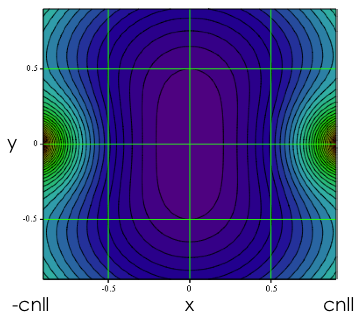
\includegraphics[width=220bp]{png/nllens_potential-2D.png}
  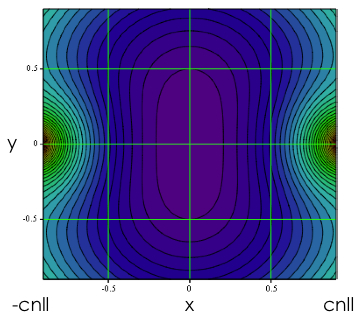
\includegraphics[width=220bp]{jpg/nllens_potential-2D.jpg}
  \caption{Contour plot of the scalar potential}
  \label{fig:nllens-potential}
\end{figure}

The multipole expansion of the scalar potential is \\
\begin{equation}
U(x,y)=k\cdot Re\left\{ \left(\dfrac{x + i y}{c}\right)^2 +
\frac{2}{3}\left(\dfrac{x + i y}{c}\right)^4 +
\frac{8}{15}\left(\dfrac{x + i y}{c}\right)^6 +
\frac{16}{35}\left(\dfrac{x + i y}{c}\right)^8 + \cdots \right\}
\end{equation}
\\
Note that this expansion is only valid inside the \textit{r=c} circle on
the x,y plane.

In order to create integrable optics, one needs to shape the potential
along z axis according to the beta-function. Below is an example
nonlinear section representing the necessary nonlinear field with 20
thin lenses:
\begin{verbatim}
    mu0 = 0.3;  ! phase advance over straight section
    l0 = 2.0;   ! length of the straight section
    nn = 20;    ! number of nonlinear elements
    tn = 0.45;  ! strength of nonlinear lens
    cn = 0.01;  ! dimentional parameter of nonlinear lens

    musect = mu0 + 0.5;
    f0 = l0/4.0*(1.0+1.0/tan(pi*mu0)^2);
    betae = l0/sqrt(1.0-(1.0-l0/2.0/f0)^2);
    alfae = l0/2.0/f0/sqrt(1.0-(1.0-l0/2.0/f0)^2);
    betas = l0*(1-l0/4.0/f0)/sqrt(1.0-(1.0-l0/2.0/f0)^2);
    value, f0, betae, alfae, betas;

    ncreate(ii,kk,cc): macro = {n.ii: nllens, knll=kk, cnll=cc;};

    i=0;
    while(i <  nn)
      {
        i = i+1;
        sn = l0/nn*(i-0.5);
        bn = l0*(1-sn*(l0-sn)/l0/f0)/sqrt(1.0-(1.0-l0/2.0/f0)^2);
        knn = l0*tn*cn^2/nn/bn;
        cnn = cn*sqrt(bn);
        exec, ncreate($i,knn,cnn);
        value, i, bn, cnn, knn;
      };
\end{verbatim}


%% To be moved in References at the end of the document
%% References:
%% \begin{enumerate}
%% \item V. Danilov, S. Nagaitsev, Phys. Rev. ST Accel. Beams \textbf{13},
%%   084002 (2010).

%% \item A. Valishev, S. Nagaitsev, V. Kashikhin, V. Danilov, in
%%   Proceedings of 2011 Particle Accelerator Conference, New York, NY,
%%   USA, WEP070.
%% \end{enumerate}

%A. Valishev, March 19, 2012


%  Changed by: Frank Schmidt, 28-Aug-2003
%  Changed by: Werner Herr, 22-May-2007
\section{Closed Orbit Corrector}
\ttindex{kicker}\index{orbit corrector}
\label{sec:closed-orbit-cor}\label{sec:kicker}

Three types of magnetic closed orbit correctors are available:
\begin{madlist}
   \ttitem{HKICKER} a corrector for the horizontal plane,
   \ttitem{VKICKER} a corrector for the vertical plane,
   \ttitem{KICKER} a corrector for both planes.
\end{madlist}

\madbox{
xxxxxxxxxxxxxxxx\=xxxxxxxxxxxxxxxxxxxx\= \kill
label: HKICKER, \>L=real, KICK=real,  \>TILT=real; \\
label: VKICKER, \>L=real, KICK=real,  \>TILT=real; \\
label: KICKER,  \>L=real, HKICK=real, \>VKICK=real, TILT=real;
}

\textbf{The type \texttt{KICKER} should not be used when an orbit corrector
  kicks only in one plane.}

The attributes have the following meaning:
\begin{madlist}
   \ttitem{L} The length of the closed orbit corrector (default: 0 m).
   \ttitem{KICK} The momentum change $\delta PX = \delta p_x/p_0$ or
     $\delta PY = \delta p_y / p_0$ for respectively horizontal or vertical
     correctors. (default: 0).
   \ttitem{HKICK} The horizontal momentum change
     $\delta PX = \delta p_x/p_0$ for a corrector acting in both planes
     (default: 0).
   \ttitem{VKICK} The vertical momentum change
     $\delta PY = \delta p_y/p_0$  for a corrector acting in both planes
     (default: 0).
   \ttitem{TILT} The roll angle about the longitudinal axis (default: 0
     rad). A positive angle represents a clockwise rotation of the
     kicker.
\end{madlist}

A positive kick increases $p_x$ or $p_y$ respectively. This
means that a positive horizontal kick bends to the left,  i.e. to
positive $x$ which is opposite of what is true for bends.

The deviation angle $\theta$ of the particle trajectory is related to
the momentum change through  $\sin \theta = \delta P = \delta p / p_0$.

It should be noted that the kick values assigned to an orbit corrector
like above are not overwritten by an orbit correction using the
\hyperref[sec:correct]{\texttt{CORRECT}}
command. Instead the kicks computed by an orbit correction and the
assigned values are added when the correctors are used.

 Examples:
\madxmp{
xxxxxxx\=xxxxxxxxxx\=xxxxxxxxxxxxxxxxx\= \kill
HK1:   \>HKICKER, \>KICK = 0.001;  \\
VK3:   \>VKICKER, \>KICK = 0.0005; \\
VK4:   \>VKICKER, \>KICK := AVK4; \\
KHV1:  \>KICKER,  \>HKICK = 0.001,   \>VKICK = 0.0005; \\
KHV2:  \>KICKER,  \>HKICK := AKHV2H, \>VKICK := AKHV2V;
}

The assignment in the form of a deferred expression has the advantage
that the values can be assigned and/or modified at any time (and
matched!).

The \hyperref[subsec:local-straight]{straight reference system} for an
orbit corrector is a Cartesian coordinate system.


Please note that there is a new feature introduced by Stefan Sorge from
GSI. Here his decription:

The elements \texttt{KICKER, HKICKER}, and \texttt{VKICKER} can also be used as
magnetic exciters providing sinusoidal momentum kicks. The usage in this case
is:

\madxmp{
xykick: KICKER,  \= SINKICK=integer, SINPEAK=real, SINTUNE=real, SINPHASE=real;  \\
xkick : HKICKER, \> SINKICK=integer, SINPEAK=real, SINTUNE=real, SINPHASE=real;  \\
ykick : VKICKER, \> SINKICK=integer, SINPEAK=real, SINTUNE=real, SINPHASE=real;
}
where a sinusoidal momentum kick \texttt{dpz} as a function of the  revolution
number \texttt{n} given by\\
\texttt{dpz(n)=SINPEAK * sin(2*PI*SINTUNE*n + SINPHASE), pz=px,py} \\
is provided.

The \texttt{KICKER} element generates synchronous kicks in both horizontal and
vertical planes. \texttt{HKICKER} generates only a horizontal kick, and
\texttt{VKICKER} generates only a vertical kick.

The variables are

\begin{madlist}
   \ttitem{SINKICK} must be set to 1 to switch on the sinusoidal
     signal, default: 0.
   \ttitem{SINPEAK} amplitude of the bending angle (rad); default: 0
     rad.
   \ttitem{SINTUNE} frequency of the signal times the revolution
     frequency.  Hence, the phase per revolution is 2*PI*SINTUNE;
     default: 0.
   \ttitem{SINPHASE} initial phase; default: 0 rad.
\end{madlist}

The momentum kick of a kicker has only a single frequency. An element
having a finite bandwidth can approximately created by defining  thin
kickers with all amplitudes \texttt{SINPEAK}, frequencies
\texttt{SINTUNE}, and initial phases \texttt{SINPHASE} desired and
putting them at the same position \textit{s} in the accelerator.

%From S.Sorge@gsi.de


%  Created by: Laurent Deniau, 15-Sep-2011
\section{Transverse Kicker}
\ttindex{tkicker}
\label{sec:tkicker}

The type \texttt{TKICKER} should be used to create horizontal, vertical or
combined transverse magnetic kickers physically equivalent to elements of type
\texttt{KICKER}, but \textbf{not used} by the \hyperref[sec:correct]{CORRECT}
command of the closed orbit correction module.

Examples of elements that may use the type \texttt{TKICKER}:
\begin{itemize}
   \item Fast kickers for injection, dump and tune
   \item Magnetic septa towards beam dump
   \item Dampers of transverse beam oscillations
   \item Undulator and Wiggler magnets
\end{itemize}

For further information on element type \texttt{TKICKER} and its attributes, look
at the documentation of the orbit corrector type
\hyperref[sec:kicker]{\texttt{KICKER}}.


\section{RF Cavity}
\ttindex{RFcavity}
\label{sec:rf-cavity}\label{sec:rfcavity}

\madbox{
label: RFCAVITY, \= L=real, VOLT=real, LAG=real, \\
                 \> FREQ=real, HARMON=integer, \\
                 \> N\_BESSEL=integer, NO\_CAVITY\_TOTALPATH=logical;
}

An \texttt{RFCAVITY} has eight real attributes and one integer attribute:
\begin{madlist}
   \ttitem{L} The length of the cavity (DEFAULT: 0 m)

   \ttitem{VOLT} The peak electrical RF voltage (DEFAULT: 0 MV). The effect of
   the cavity is \\
     delta(\textit{E}) = VOLT * sin(2$\pi$ * (LAG - HARMON * \textit{f$_0$ t})).

   \ttitem{LAG} The phase lag [$2\pi$] (DEFAULT: 0).

   \ttitem{FREQ} The frequency [MHz] (no DEFAULT).  \\[3mm]
   \textbf{Note that if the RF frequency is not given, it is computed
     from the harmonic number and the revolution frequency
     \textit{f$_0$}. For accelerating structures this makes no sense,
     and the input of the frequency is mandatory.}

   \ttitem{HARMON} The harmonic number \textit{h} (no DEFAULT). This
   attribute is only used if the frequency is not given.
\end{madlist}

\textbf{Caveats:}
\begin{itemize}
  \item Please take note, that the following \madeight attributes:
    \texttt{BETRF, PG, SHUNT} and \texttt{TFILL} are currently not implemented in
    \madx.
%  \item BETRF: RF coupling factor (DEFAULT: 0).
%  \item PG: The RF power per cavity (DEFAULT: 0 MW).
%  \item SHUNT: The relative shunt impedance (DEFAULT: 0 MOhm/m).
%  \item TFILL: The filling time of the cavity $T_{fill}$ (DEFAULT: 0 microseconds).

  \item Important Note: The \hyperref[chap:twiss]{\texttt{TWISS}} command
    is 4D only. As a consequence the \texttt{TWISS} parameters in the plane
    of non-zero dispersion may not close as expected. Therefore, it is best
    to perform \texttt{TWISS} in 4D only, \textsl{i.e.} with cavities
    switched off. If 6D is needed one has to use the
    \hyperref[sec:ptc-twiss]{\texttt{PTC\_TWISS}} command.
    Please refer to \hyperref[sec:ptc-setswitch]{\texttt{PTC\_SETSWITCH}} command,
    in particular to \texttt{TIME} and \texttt{TOTALPATH} switches,
    concerning RF behaviour of cavities in PTC.

  \item The charge is not taken into account by the RF-cavity.
  
  \item The RF-cavity has to be thin for TRACKING in MAD-X. This is handled by 
  \texttt{MAKETHIN} but note that it is always sliced into a single slice.  

\end{itemize}

The \texttt{RFCAVITY} can also have attributes that only become active in
\ptc:
\begin{madlist}
   \ttitem{N\_BESSEL} (DEFAULT: 0): \\
     Transverse focussing effects are typically ignored in the cavity in
     \madx or even \ptc. This effect is being calculated to order
     \texttt{n\_bessel}, with \texttt{n\_bessel=0} disregarding this
     effect and with a correct treatment when \texttt{n\_bessel} goes to
     infinity.
   \ttitem{NO\_CAVITY\_TOTALPATH} (Default: false): \\
     flag to select whether the transit time factor in the cavity is to be
     considered (\texttt{NO\_CAVITY\_TOTALPATH = false}) or if the particle is
     kept on constant RF phase when passing through cavity. (\texttt{NO\_CAVITY\_TOTALPATH = true}).
\end{madlist}

A cavity requires the particle \hyperref[sec:beam]{\texttt{ENERGY}}
and the particle \hyperref[sec:beam]{\texttt{CHARGE}} to be set by a
\hyperref[sec:beam]{\texttt{BEAM}} command before any calculations are
performed.

Example:
\madxmp{
BEAM, PARTICLE=ELECTRON, ENERGY=50.0; \\
CAVITY: RFCAVITY, L=10.0, VOLT=150.0, LAG=0.0, HARMON=31320;
}

The \hyperref[subsec:local-straight]{straight reference system} for a
cavity is a Cartesian coordinate system.

%%%%%%%%%%%%%%%%%%%%%%%%%%%%%%%%%%%%%%%%%%%%%%%%%%%

\section{Travelling Wave Cavity}
\ttindex{TWcavity}
\label{sec:tw-cavity}\label{sec:twcavity}

\madbox{
label: TWCAVITY, \= L=real, VOLT=real, FREQ=real, LAG=real, \\
                 \> PSI=real, DELTA\_LAG=real ;
}

The travelling wave cavities model the accelerating structures of linacs
where wavefront moves together with the accelerated particles.
This element is implemented only by PTC and is treated as drift
by native MADX commands. The phase velocity is fixed to speed of light
and can not be varied.

\begin{madlist}
   \ttitem{L} The length of the cavity (DEFAULT: 0 m)

   \ttitem{VOLT} The peak electrical RF voltage (DEFAULT: 0 MV).

   \ttitem{FREQ} The frequency [MHz] (no DEFAULT).  \\[3mm]

   \ttitem{LAG} The phase lag [$2\pi$] (DEFAULT: 0). Zero lag means the highest acceleration,
                i.e. the reference particle (starting at x=0, px=0, y=0, py=0,t=0, pt=0)
                is on the crest of the wave. Please note that it is different from
                the \texttt{RFCAVITY} nomenclature.

   \ttitem{PSI}

   \ttitem{DELTA\_LAG}
\end{madlist}

%%%%%%%%%%%%%%%%%%%%%%%%%%%%%%%%%%%%%%%%%%%%%%%%%%%



\section{Thin Radio-Frequency Multipole}
\ttindex{rfmultipole}
\label{sec:rfmultipole}

\madbox{
xxxxxxxxxxxxxxxxxxxxx\= \kill
label: RFMULTIPOLE, \>L=real, VOLT=real, LAG=real, \\
       \> FREQ=real, HARMON=integer, \\
       \> LRAD=real, TILT=real, \\
       \> KNL=\{real, \ldots \}, KSL=\{real, \ldots \}, \\
       \> PNL=\{real, \ldots \}, PSL=\{real, \ldots \};
}

A \texttt{RFMULTIPOLE} is a element which exhibits the properties
of an RF cavity as well as those of a multipole, of arbitrary order, oscillating at
the same RF frequency.

The accelerating kick is \texttt{delta(E) = VOLT * sin(2$\pi$ * (LAG - HARMON *
f0 t))}, and the multipole moments oscillate with the same RF frequency.

An \texttt{RFMULTIPOLE} requires the particle
\hyperref[sec:beam]{\texttt{ENERGY}} and the particle
\hyperref[sec:beam]{\texttt{CHARGE}} to be set with a
\hyperref[sec:beam]{\texttt{BEAM}} command before any calculation is
performed.

Contrary to the regular multipole, where the dipole
component has an effect on the reference orbit, an RF-Multipole that
includes a dipole component does not bend the reference orbit.

In PTC there must be at least one cavity with non-zero voltage,
otherwise all RF elements, including RF multipoles, are disabled.
Concerning RF behaviour of cavities in PTC
please refer to \hyperref[sec:ptc-setswitch]{\texttt{PTC\_SETSWITCH}} command,
in particular to \texttt{TIME} and \texttt{TOTALPATH} switches.


\begin{madlist}
   \ttitem{VOLT} The peak voltage of the RF accelerating mode (DEFAULT: 0 MV).
   \ttitem{LAG} The phase lag [$2\pi$] (DEFAULT: 0)
   \ttitem{FREQ} The frequency [MHz] (no DEFAULT). \\
     Note that if the RF
     frequency is not given, it is computed from the harmonic
     number and the revolution frequency f0 as before. However, for
     accelerating structures this makes no sense, and the frequency
     is mandatory.
   \ttitem{HARMON} The harmonic number h (no DEFAULT). Only if the
     frequency is not given.
   \ttitem{LRAD} A fictitious length, which was originally just used to
     compute synchrotron radiation effects.
   \ttitem{TILT} The roll angle about the longitudinal axis (default: 0
     rad). A positive angle represents a clockwise rotation of the
     multipole element.

     \textbf{Please note that contrary to \madeight one has to specify the
       desired \texttt{TILT} angle, otherwise it is taken as 0 rad. We
       believe that the \madeight concept of having individual
       \texttt{TILT} values for each component and on top with default
       values led to considerable confusion and allowed for excessive
       and unphysical freedom. Instead, in \madx the \texttt{KNL, KSL}
       components can be considered as the normal or skew
       multipole components of the magnet on the bench, while the
       \texttt{TILT} attribute can be considered as an tilt alignment
       error in the machine.}

   \ttitem{KNL} An array of the integrated normal rfmultipole
     coefficients, starting from order zero and up to the maximum
     order (currently 20).
     The parameters are positional in the array, therefore leading
     zeros must be filled in for components that do not exist.
%     The normal rfmultipole coefficients from order zero to
%     the maximum; the parameters are positional, therefore zeros
%     must be filled in for components that do not exist. Example of
%     a thin-lens sextupole: ms:rfmultipole, knl:=\{0, 0, k2l\};
   \ttitem{KSL} An array of the integrated skew rfmultipole
     coefficients, starting from order zero and up to the maximum
     order (currently 20).
     The parameters are positional in the array, therefore leading
     zeros must be filled in for components that do not exist.
%     The skew rfmultipole coefficients from order zero to
%     the maximum; the parameters are positional, therefore zeros
%     must be filled in for components that do not exist. Example of
%     a thin-lens skew octupole:
   \ttitem{PNL} The phase for each normal rfmultipole coefficients from
     order zero to the maximum; the parameters are positional,
     therefore leading zeros must be filled in for components that do not
     exist.
   \ttitem{PSL} The phase for each skew rfmultipole coefficients from
     order zero to the maximum; the parameters are positional,
     therefore leading zeros must be filled in for components that do not
     exist.
\end{madlist}

\textbf{Examples}
\begin{itemize}
	\item A skew RF octupole
	\madxmp{MS: RFMULTIPOLE, KSL=\{0, 0, 0, k3sl\};}

Notice that both \texttt{KNL} and \texttt{KSL} for the same multipole mode can be specified simultaneously.

\item An \texttt{RFMULTIPOLE} used as a \texttt{CRABCAVITY}:
	\madxmp{rfdipole: RFMULTIPOLE, \=L=Lcrab, KNL=\{ Vcrab / PC0 \}, \\
								   \>PNL=\{ 0.25 + LAGcrab \};}

is equivalent to

	\madxmp{crab: CRABCAVITY,  \=L=Lcrab, VOLT=Vcrab, LAG=LAGcrab;}

\end{itemize}

%  Added by: R. Calaga, Sep 2010
%  Edited by: A. Latina, Jun 2013
\section{Crab Cavity}
\ttindex{crabcavity}
\label{sec:crab-cavity}\label{sec:crabcavity}

\madbox{
label: CRABCAVITY, \=L=real, TILT=real, VOLT=real, LAG=real, \\
                   \>FREQ=real, HARMON=integer, \\
                   \>RV1=integer, RV2=integer, \\
                   \>RV3=integer, RV4=integer, \\
                   \>RPH1=integer, RPH2=integer, LAGF=real ;
}

A \texttt{CRABCAVITY} has six attributes describing its steady state
and seven attributes to describe dynamic behaviour:

\begin{madlist}
  \ttitem{L} The length of the cavity (default: 0 m)

  \ttitem{TILT} The tilt of the cavity in radian (default: 0 m). If the tilt is $\pi/2$, then the export to sixtrack will automatically convert it to a vertical cravity (default is horizontal).

  \ttitem{VOLT} The peak RF voltage (default: 0 MV).

  \ttitem{LAG} The initial phase lag [$2\pi$] (default: 0).

  \ttitem{FREQ} The RF frequency [MHz] (no default). \\[3mm]
    \textbf{Note that if the RF frequency is not given, it is computed from the
    harmonic number and the revolution frequency \textit{f$_0$}.
    For deflecting structures this makes no sense, and the
    frequency is mandatory.}

  \ttitem{HARMON} The harmonic number \textit{h} (no default). \\
  Only if the frequency is not given.

% \item BETRF: RF coupling factor (default: 0).
% \item PG: The RF power per cavity (default: 0 MW).
% \item SHUNT: The relative shunt impedance (default: 0 MOhm/m).
% \item TFILL: The filling time of the cavity T<sub>fill</sub> (default: 0 microseconds).
%\item EPHASE: Value of the final crab RF phase [2pi] with respect to  nominal value (default: 0).
\end{madlist}

The other attributes describe the time evolution of a \texttt{CRABCAVITY} behaviour:

\begin{madlist}
  \ttitem{RV1} Number of initial turns with zero voltage (default: 0).
  \ttitem{RV2} Number of turns to ramp voltage from zero to nominal value (default: 0).
  \ttitem{RV3} Number of turns with nominal voltage (default: 0).
  \ttitem{RV4} Number of turns to ramp voltage from nominal value to zero (default: 0).

  \ttitem{LAGF} Value of the final crab RF phase lag [$2\pi$] (default: 0).

  \ttitem{RPH1} Number of initial turns with nominal phase (default: 0).
  \ttitem{RPH2} Number of turns to ramp phase [$2\pi$] from nominal to
    specified value \\ (default:~0).

\end{madlist}

\textbf{Caveats:}
\begin{itemize}
   \item Please take note, that the following \madeight attributes:
     \texttt{BETRF, PG, SHUNT} and \texttt{TFILL} are currently not
     implemented in \madx!
   \item Note that crab cavities are only implemented for
     tracking  purposes. \\
     \hyperref[chap:twiss]{\texttt{TWISS}} ignores any effect of the
     crab cavity.
   \item Important Note: The \hyperref[chap:twiss]{\texttt{TWISS}} command
     is 4D only. As a consequence the \texttt{TWISS} parameters in the plane
     of non-zero dispersion may not close as expected. Therefore, it is best
     to perform \texttt{TWISS} in 4D only, \textsl{i.e.} with cavities
     switched off. If 6D is needed one has to use the
     \hyperref[sec:ptc-twiss]{\texttt{PTC\_TWISS}} command.
\end{itemize}

%A cavity requires the particle energy (\href{beam.html#energy}{ENERGY})
%and the particle charge (\href{beam.html#charge}{CHARGE}) to be set by
%a \href{beam.html}{BEAM} command before any calculation is performed.

Before any calculation is performed with a \texttt{CRABCAVITY}, the particle
\hyperref[sec:beam]{\texttt{ENERGY}} and the particle
\hyperref[sec:beam]{\texttt{CHARGE}} must be set with the
\hyperref[sec:beam]{\texttt{BEAM}} command.

The effect of a \texttt{CRABCAVITY} on particle coordinates during tracking is
\\
\\ $\mathtt{\delta p_x  = VOLT * \sin(PHI - OMEGA * t)}$
\\ $\mathtt{\delta E  = - VOLT * OMEGA * x * \cos (PHI - OMEGA * t)}$
\\
\\ where $\mathtt{PHI =  2\pi * (LAG - HARMON * f_0 t)}$,
\\ and $\mathtt{OMEGA = 2\pi * FREQ / c}$
\\
% delta(<i>E</i>) = VOLT *
% sin(2 pi * (LAG - HARMON * <i>f<sub>0</sub> t</i>)).


Example:
\madxmp{
xxxxxxxx\= \kill
BEAM, PARTICLE=PROTON, ENERGY=7000.0; \\
CAVITY:  \>CRABCAVITY, L=10.0, VOLT=5.0, LAG=0.0, FREQ=400, \\
         \>RV1=0, RV2=50, RV3=1000, RV4=50, \\
         \>RPH1=100, RPH2=500, LAGF=0.125;
}

The \hyperref[subsec:local-straight]{straight reference system} for a
cavity is a Cartesian coordinate system.

%\href{http://www.cern.ch/rcalaga}{R. Calaga}, September 2010



%%%%%%%%%%%%%%%%%%%%%%%%%%%%%%%%%%%%%%%%%%%%%%%%%%%%%%


\section{AC Dipole}
\ttindex{acdipole}\index{ac dipole}
\label{sec:acdipole}

Alternating Current (AC) dipole is implemented with:
\begin{madlist}
   \ttitem{HACDIPOLE} an AC dipole for the horizontal plane,
   \ttitem{VACDIPOLE} an AC dipole for the vertical plane,
\end{madlist}

\madbox{
xxxxxxxxxxxxxxxx\=xxxxxxxxxxxxxxxxxxxx\= \kill
label: HACDIPOLE, L=real, VOLT=real,  FREQ=real, LAG=real, \\
                  \> RAMP1=integer, RAMP2=integer, \\
                  \> RAMP3=integer, RAMP4=integer; \\
label: VACDIPOLE, L=real, VOLT=real,  FREQ=real, LAG=real, \\
                  \> RAMP1=integer, RAMP2=integer, \\
                  \> RAMP3=integer, RAMP4=integer;
}
In fact this element is rather oscilating (time varying) orbit corrector (kicker) rather than dipole
because it does not change the reference frame. The oscillation is assumed to be slow
compared with bunch length and the kick is constant along the bunch.
These devices are used for beam excitations in circular machines for optics measurements.
They are linearly ramped up to the full amplitude (and ramped down)
to avoid emittance growth.

The attributes have the following meaning:
\begin{madlist}
   \ttitem{L} The length of the device (default: 0 m).
   \ttitem{VOLT} The amplitude of the kick
     (default: 0).
   \ttitem{FREQ} Tune of the oscillation in $2\pi$ units. \\
     \textbf{The name of the parameter is misleading and will be changed in the future for TUNE.} \\
     (default: 0).
   \ttitem{RAMP1} Starting turn of amplitude ramp-up. \\
     (default: 0).
   \ttitem{RAMP2} Last turn of amplitude ramp-up. \\
     (default: 0).
   \ttitem{RAMP3} Starting turn of amplitude ramp-down. \\
     (default: 0).
   \ttitem{RAMP4} Last turn of amplitude ramp-down. \\
     (default: 0).
\end{madlist}


AC dipole is not implemented in \texttt{TWISS}.

In \texttt{TRACK} it is implemented as a zero-length element
changing transverse momentum by $(0.3 \cdot VOLT / p0c) \cdot sin(2\pi \cdot FREQ  \cdot turn)$,
where $turn$ is turn number. If ramp settings are left with default values (all zero)
AC dipole has no effect in \texttt{TRACK}.

PTC requires that \texttt{MODULATION} flag is set to true
via \texttt{PTC\_SETSWITCH} command to enable AC dipole,
otherwise it is treated as a drift.

For computation of the maps in \texttt{PTC\_TWISS} and \texttt{PTC\_NORMAL}
the phasespace is than extended by extra dimensions corresponding to
the frequency clocks defined with AC dipoles.
Maximum of three distinct frequencies are allowed.
There can be more then three AC dipoles but than some of them need to have
the same frequencies.
\texttt{PTC\_TWISS}, when invoked with \texttt{NORMAL=true}, calculates
dependence of optical paramters on amplitudes of the clocks.
Results of \texttt{PTC\_TRACK} and \texttt{PTC\_TRACKLINE}
may be slightly different from \texttt{TRACK} because of some implementation details,
in particular for not fully relativistic beams.
PTC internaly uses frequency so time of flight effects are taken into account
and kick amplitude is inversely proportional to relativistic beta function.
Please note that at the moment \texttt{LAG} parameter is ignored
in translation to PTC. If ramp settings are left with default values (all zero)
PTC tracking will assume maximum amplitude.


%%%%%%%%%%%%%%%%%%%%%%%%%%%%%%%%%%%%%%%%%%%%%%%%%%%%%%



\section{Electrostatic Separator}
\ttindex{elseparator}
\label{sec:separator}\label{sec:elseparator}

\madbox{
label: ELSEPARATOR, L=real, EX=real, EY=real, TILT=real;
}

An \texttt{ELSEPARATOR} element has four real attributes:
\begin{madlist}
   \ttitem{L} The length of the separator (default: 0 m).
   \ttitem{EX} The horizontal electric field strength (default: 0 MV/m).
     A positive field increases \textit{p$_x$} for positive particles.
   \ttitem{EY} The vertical electric field strength (default: 0 MV/m).
     A positive field increases \textit{p$_y$} for positive particles.
   \ttitem{TILT} The roll angle about the longitudinal axis (default: 0
     rad). A positive angle represents a clockwise of the electrostatic
     separator.
   \ttitem{EX\_L} The integrated vertical electric field strength (default: 0 MV).
    This parameter is only used in \hyperref[sec:trackoverview]{\texttt{THINTRACK}} and ignored by \hyperref[chap:twiss]{\texttt{TWISS}}.
   \ttitem{EY\_L}  The integrated horizontal electric field strength (default: 0 MV).
    This parameter is only used in \hyperref[sec:trackoverview]{\texttt{THINTRACK}} and ignored by \hyperref[chap:twiss]{\texttt{TWISS}}.
\end{madlist}
An electrostatic separator requires the particle \texttt{ENERGY} and the
particle \texttt{CHARGE} to be set by a
\hyperref[sec:beam]{\texttt{BEAM}} command before any calculation is
performed. Note that no thin elseparator currently exists in \hyperref[chap:twiss]{\texttt{TWISS}}.
Example:
\madxmp{
BEAM, PARTICLE=positron, ENERGY=50.0;\\
SEP: ELSEPARATOR, L=5.0, EY=0.5;
}

The \hyperref[subsec:local-straight]{straight reference system} for a
separator is a Cartesian coordinate system.


\section{Beam Position Monitor}
\label{sec:monitor}

A beam monitor has no specific effect on the beam and behaves like a
drift space.
In addition it serves to record the beam position for closed orbit
correction.

Three different types of beam position monitors are recognised:
\begin{madlist}
   \ttitem{HMONITOR} Monitor for the horizontal beam position,
   \ttitem{VMONITOR} Monitor for the vertical beam position,
   \ttitem{MONITOR} Monitor for both horizontal and vertical beam position.
\end{madlist}

\madbox{
label: HMONITOR, \=   L=real; \\
label: VMONITOR, \>   L=real; \\
label: MONITOR,  \>   L=real;
}

A beam position monitor has one real attribute:
\begin{madlist}
   \ttitem{L} The length of the monitor (default: 0 m).
     %% If the length is different from zero, the beam position is recorded
     %% in the centre of the monitor.
\end{madlist}

Examples:
\madxmp{
MH: HMONITOR, L = 1; \\
MV: VMONITOR;
}

The \hyperref[subsec:local-straight]{straight reference system} for a
monitor is a Cartesian coordinate system.

\section{Instrument and Placeholder}
\label{sec:instrument}
\label{sec:placeholder}
An instrument or a placeholder has no specific effect on the beam and
behaves like a drift space.
An instrument is different from beam a position monitor and is not used
for closed orbit correction.

Two different types of instruments are recognised:

\begin{madlist}
   \ttitem{INSTRUMENT} A place holder for any type of beam
     instrumentation. Optically it behaves like a drift space; it
     returns \emph{no beam observation}. It represent a class of
     elements which is completely independent from drifts and monitors.
   \ttitem{PLACEHOLDER} A place holder for any type of
     element. Internally it is equivalent to an \texttt{INSTRUMENT}:
     optically it behaves as a drift space, it returns
     \emph{no beam observation}. It represent a class of elements
     which is completely independent from drifts and monitors.
\end{madlist}

\madbox{
xxxxxxxxxxxxxxxxxxxxx\= \kill
label: INSTRUMENT,   \>L=real; \\
label: PLACEHOLDER,  \>L=real;
}

An instrument or placeholder has one real attribute:
\begin{madlist}
   \ttitem{L} The length of the instrument (default: 0 m).
\end{madlist}

The \hyperref[subsec:local-straight]{straight reference system} for an
instrument is a Cartesian coordinate system.


\section{Collimator}
\label{sec:collimator}

A \texttt{COLLIMATOR} has no specific effect on beam optics and behaves like a
\hyperref[sec:drift]{drift space}.

\madbox{
label: COLLIMATOR, \=L=real, \\
                   \>APERTYPE=string,  APERTURE=\{values\}, \\
                   \>APER\_OFFSET=\{values\}, APER\_TOL=\{values\};
}

A \texttt{COLLIMATOR} has one specific real attribute:
\begin{madlist}
  \ttitem{L} The collimator length (default: 0 m).
\end{madlist}

Additionally, like any other element, except \texttt{DRIFT} space,
a \texttt{COLLIMATOR} can have specific aperture related attributes
as defined in the related section \hyperref[sec:def-aper]{Defining
aperture in \madx}

During \hyperref[chap:thintrack]{tracking} in \madx, particle loss
is checked at the entrance of the element by comparing the particle coordinates
and the defined aperture, provided that the \texttt{APERTURE} flag is \texttt{true}
in the \hyperref[sec:track]{\texttt{TRACK}} command,
and that the \texttt{APERTYPE} attribute value of the element is one of the
predefined types.
An aperture model defined in an external file (\texttt{APERTYPE=filename})
is not used to check particle loss during tracking.

Example:
\madxmp{
COLLIM: COLLIMATOR, L=0.5, APERTYPE=ellipse, APERTURE={0.01,0.005};
}

The \hyperref[subsec:local-straight]{straight reference system} for a
collimator is a Cartesian coordinate system.

\textbf{NOTE:} A collimator can be displaced transversally in order to
model an asymmetric collimator by means of the \texttt{APER\_OFFSET} attributes;
During tracking particle losses are then reported with coordinates with respect
to the \textbf{displaced} reference system, not with respect to the surrounding
beam line.

Other collimator elements have been inherited from \madeight and still exist
in \madx for backward compatibility.
\texttt{ECOLLIMATOR} (elliptic aperture collimator) and \texttt{RCOLLIMATOR}
(rectangular aperture collimator) behave both as drift spaces in \madx
They are declared with

\madbox{
  label: ECOLLIMATOR, L=real, XSIZE=real, YSIZE=real; \\
  label: RCOLLIMATOR, L=real, XSIZE=real, YSIZE=real;
}

Either type has several real attributes:
\begin{madlist}
  \ttitem{L} The collimator length (default: 0 m).
  \ttitem{XSIZE} The horizontal half-aperture (default: unlimited). \\
  \textbf{OBSOLETE : parsed and stored but not used.}
  \ttitem{YSIZE} The vertical half-aperture (default: unlimited). \\
  \textbf{OBSOLETE : parsed and stored but not used.}
\end{madlist}

Users are STRONGLY advised to replaced all instances of \texttt{RCOLLIMATOR}
and \texttt{ECOLLIMATOR} in input files with appropriate \texttt{COLLIMATOR}
elements. The \texttt{RCOLLIMATOR} and \texttt{ECOLLIMATOR} elements are only
kept for the time being for backward compatibility and will be removed in
the near future.

Note also that the \texttt{XSIZE} and \texttt{YSIZE} parameters can be declared
but are simply ignored both in the \hyperref[chap:aperture]{\texttt{APERTURE}}
command an in \hyperref[chap:thintrack]{tracking}.


%  Changed by: Stefan Sorge, 2007
\section{Beam-beam Interaction}
The BEAMBEAM element may be inserted in a beam line to simulate a
beam-beam interaction point:

\madbox{
label: BEAMBEAM, \= CHARGE=real, \\
                 \> XMA=real, YMA=real, \\
                 \> SIGX=real, SIGY=real, WIDTH=real,\\
                 \> BBSHAPE=integer, BBDIR=integer;
}

The beam-beam interaction is represented by a four-dimensional
interaction with a thin element, i.e. horizontal and vertical non-linear kicks.
The code for this element has been contributed by J.M.~Veuillen (1987)
and extended by S.~Sorge (2007).

\begin{madlist}
   \ttitem{CHARGE}
     The charge of particles in the opposite beam, in elementary charges.
     \\ (default: +1) \\
     In order to describe interactions between beams containing the same
     particles and having a charge different from +1, one should set the
     \texttt{CHARGE} explicitly in the
     \hyperref[sec:beam]{\texttt{BEAM}} command as well as in the
     \texttt{BEAMBEAM} element.

   \ttitem{XMA}
     The horizontal displacement of the opposite beam with respect to
     the ideal orbit (default: 0 m).
   \ttitem{YMA}
     The vertical displacement of the opposite beam with respect to
     the ideal orbit (default: 0 m).

   \ttitem{SIGX}
     The horizontal extent of the opposite beam (default: 1 m).
     Meaning depends on parameter \texttt{BBSHAPE}.
   \ttitem{SIGY}
     The vertical extent of the opposite beam (default: 1 m).
     Meaning depends on parameter \texttt{BBSHAPE}.

   \ttitem{WIDTH} The extent of the edge region, relative to the
     \texttt{SIGX, SIGY} parameters. The absolute value is given by
     \texttt{WIDTH*SIGX} and \texttt{WIDTH*SIGY} in horizontal and
     vertical directions respectively.


   \ttitem{BBSHAPE} A parameter to select the radial density shape of the
     opposite beam \\ (default: 1)
     \begin{itemize}
       \item  \texttt{BBSHAPE=1}: Gaussian shape (default).
         \texttt{SIGX, SIGY} are the standard deviations in horizontal
         and vertical directions. \texttt{WIDTH} is ignored.

       \item  \texttt{BBSHAPE=2}: trapezoidal shape (see
       fig.\ref{fig:beambeam-n-trapez}). \texttt{SIGX, SIGY} are the half widths of
       density profile, \textsl{i.e.} distance from the centre to half
       edge region with linear decrease of density in horizontal and
       vertical directions. \\
       Only circular opposite beam is possible, \textsl{i.e.} in the
       calculations \texttt{SIGX' = SIGY' = (SIGX+SIGY)/2} is used, if
       \texttt{SIGX} and \texttt{SIGY} have different values. \\
       \texttt{WIDTH} denotes the full width of the edge
       region in units of \texttt{SIGX} (or \texttt{SIGX'} and \texttt{SIGY'},
       respectively, if \texttt{SIGX} and \texttt{SIGY} are not equal), \textsl{i.e.}
       if \texttt{WIDTH=0.01} and \texttt{SIGX=5}mm, the edge region has a full
       width of 0.05\ mm.  Condition: \texttt{WIDTH \textless 2.0}.

\begin{figure}[h]
  \centering
  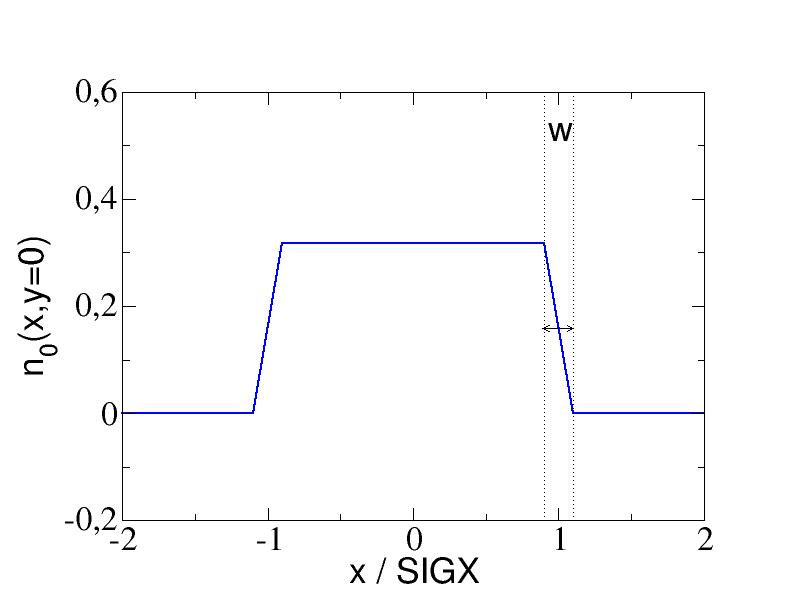
\includegraphics[width=400bp]{jpg/beambeam_n_trapez.jpg}
  \caption{Trapezoidal shape of radial density for beam-beam lens.}
  \label{fig:beambeam-n-trapez}
\end{figure}

       \item  \texttt{BBSHAPE=3}: hollow-parabolic shape (see
       fig.\ref{fig:beambeam-n-hollowparabol}). \texttt{SIGX, SIGY} are
       the distances from the centre to the maximum of the parabolic
       density profile in horizontal and vertical directions. \\
       Only circular opposite beam is possible, \textsl{i.e.} in the
       calculations \texttt{SIGX' = SIGY' = (SIGX+SIGY)/2} is
       used, if \texttt{SIGX} and \texttt{SIGY} have different
       values. \\
       \texttt{WIDTH} denotes the full width at half
       maximum of the parabolic density profile in units of
       \texttt{SIGX}, or \texttt{SIGX'} and \texttt{SIGY'},
       respectively, if \texttt{SIGX} and \texttt{SIGY} are
       not equal. Condition: \texttt{WIDTH \textless SQRT(2.0)}

\begin{figure}[h]
  \centering
  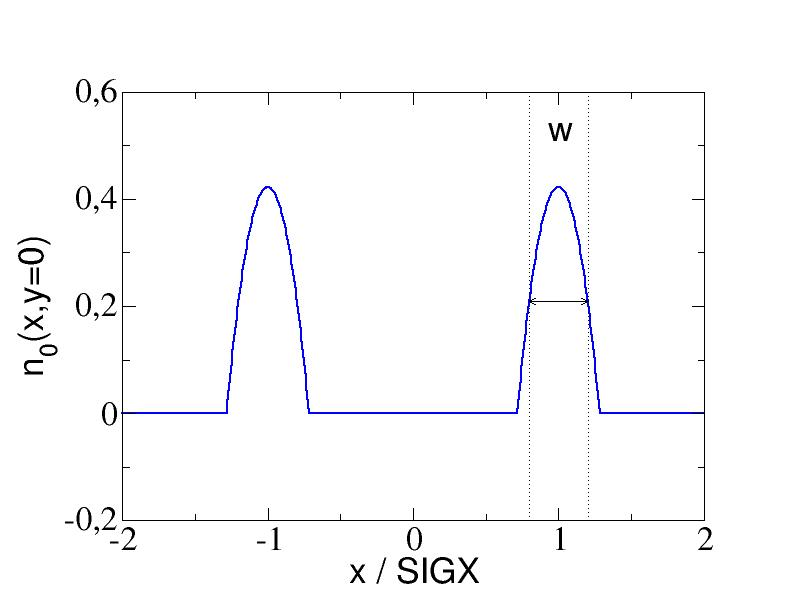
\includegraphics[width=420bp]{jpg/beambeam_n_hollowparabol.jpg}
  \caption{Hollow parabolic shape of radial density for beam-beam lens.}
  \label{fig:beambeam-n-hollowparabol}
\end{figure}

     \end{itemize}

     The restriction to circular opposite beams in the cases \texttt{BBSHAPE=2,3}
     appears to be sufficient, because such beam profiles are more important
     for the description of the interaction between the particle beam and
     an electron beam of an electron cooler, which are usually circular.


   \ttitem{BBDIR} A parameter to select the direction of motion of the
     opposite beam relative to the beam being studied. It determines
     the sign of the Lorentz force between both beams (default: -1):
     \begin{itemize}
        \item  \texttt{BBDIR=-1}: Beams move in opposite directions as in a
        collider. The Lorentz force enhances the beam-beam interaction.
        \item  \texttt{BBDIR=0}: Opposite beam does not move. The Lorentz force is
        neglected
        \item  \texttt{BBDIR=1}: Beams move in the same direction as in an
        electron cooler. The Lorentz force reduces the beam-beam interaction.
     \end{itemize}
     Note:
     \begin{itemize}
        \item  The particles in the beam considered may have a momentum
        deviation given by \texttt{DELTAP} defined in the
        \hyperref[sec:track]{\texttt{TRACK}} command.
        \item  The opposite beam is assumed to have the velocity according to
        the unperturbed energy of the particles in the beam considered. Only
        the direction of motion can be chosen.
        \item  In the case of motion in the opposite direction
        (\texttt{BBDIR=-1}), the time of interaction between the beams
        is given by \texttt{tau=length/(2*beta*clight)}, where
        \texttt{length} is the length of a bunch in the opposite beam.
        In the case of motion in the same direction (\texttt{BBDIR=1})
        as in an electron cooler, this time is given by
        \texttt{tau=length/(beta*c\_light)}, where \texttt{length} is
        the length of the cooler. Note that the factor 1/2 is inserted
        only for \texttt{BBDIR=-1} to calculate correct results.
     \end{itemize}

\end{madlist}


A beam-beam element requires the particle
\hyperref[sec:beam]{\texttt{ENERGY}} and the particle
\hyperref[sec:beam]{\texttt{CHARGE}}, as well as the number of particles
per bunch (\hyperref[sec:beam]{\texttt{NPART}}) to be set by a
\hyperref[sec:beam]{\texttt{BEAM}} command before any
calculation is performed.

Example of a four-dimensional beam-beam element definition in Collider
regime:
\madxmp{
beam,   particle = positron, npart = 1.e12, energy = 50.0; \\
bb:     beambeam, sigx = 1.e-3, sigy = 5.e-4, charge = 1.;
}


Example of a four-dimensional beam-beam element definition in an
Electron cooler:
\madxmp{
gamma0 = 1.032;                          \= ! relativistic factor \\
beta0 = sqrt(1.0-1.0/gamm0/gamma0);      \>  \\
\> \\
i\_e = 0.2;                              \> ! electron current \\
re\_cool = 0.01;                         \> ! electron beam radius \\
l\_cool = 5.0;                           \> ! cooling length \\
\\
nelect = i\_e*l\_cool/beta0/clight/qelect; ! electron number in e-cooler \\
\\
beam, particle=antiproton, gamma=gamma0, npart=nelect;  \\
bb\_ecool: beambeam, sigx=re\_cool, sigy=re\_cool, bbshape=2, \\
\hskip 4.2cm                     width=0.01, charge=-1, bbdir=1;
}


%  Changed by: Frank Schmidt, 25-June-2003
\section{Arbitrary Matrix Element}

\madbox{
label: MATRIX, \= TYPE=string, L=real,  \\
               \> KICK1=real,..., KICK6=real, \\
               \> RM11=real, ..., RM66=real, \\
               \> TM111=real, ..., TM666=real;
}

The \texttt{MATRIX} element allows the definition of an arbitrary transfer matrix.
It has four real array attributes:
\begin{madlist}
   \ttitem{L} Length of the element, which may be zero.
   \ttitem{KICKi} Defines the kick of the element acting on the six phase
     space coordinates.
   \ttitem{RMik} Defines the linear transfer matrix ($6\times6$ terms) of the element.
   \ttitem{TMikl} Defines the second-order terms ($6\times6\times6$ terms) of the element.
\end{madlist}

Data values that are not explicitly entered are taken from the identity
transformation for the \texttt{RMik} matrix elements, and taken as zero
for the \texttt{KICKi} kick factors and the \texttt{TMikl} second order
terms.
In the \hyperref[chap:thintrack]{thin-lens tracking
module} a non-zero length for an arbitrary matrix is accepted, however
no non-zero second order terms are allowed to avoid non symplectic
tracking runs. In the latter case the tracking run is aborted.


%\section{Coordinate Transformations}
\section{Rotation around the vertical axis}
\label{sec:yrotation}

The element \texttt{YROTATION} rotates the
\hyperref[subsec:local-straight]{straight reference system} about the
vertical (\textit{y}) axis.

\madbox{
label: YROTATION, ANGLE=real;
}

\texttt{YROTATION} has no effect on the beam, but it
causes the beam to be referred to the new coordinate system  \\
\begin{equation}\begin{split}
x_2 &= x_1 \cos\theta - s_1 \sin\theta \\
s_2 &= x_1 \sin\theta + s_1 \cos\theta
\end{split}\end{equation}
%%\textit{x}$_2$=\textit{x}$_1$cos(theta)-\textit{s}$_1$sin(theta), \\
%%\textit{y}$_2$=\textit{x}$_1$sin(theta)+\textit{s}$_1$cos(theta).\\

It has one real attribute:
\begin{madlist}
   \ttitem{ANGLE} The rotation angle $\theta$ (default: 0 rad).
\end{madlist}

A positive angle means that the new reference system is rotated
clockwise about the local \textit{y}-axis with respect to the old system.

\textbf{Important note:} \\
The rotation angle $\theta$ must be \emph{small}, \textsl{i.e.} it must be at
most comparable to the transverse angles of the orbit.

Example:
\madxmp{
KINK: YROTATION, ANGLE = 0.0001;
}

\section{Rotation around the horizontal axis}
\label{sec:xrotation}

The element \texttt{XROTATION} rotates the
\hyperref[subsec:local-straight]{straight reference system} about the
vertical (\textit{x}) axis.

\madbox{
	label: XROTATION, ANGLE=real;
}

\texttt{XROTATION} has no effect on the beam, but it
causes the beam to be referred to the new coordinate system  \\
\begin{equation}\begin{split}
y_2 &= y_1 \cos\theta - s_1 \sin\theta \\
s_2 &= y_1 \sin\theta + s_1 \cos\theta
\end{split}\end{equation}
%%\textit{x}$_2$=\textit{x}$_1$cos(theta)-\textit{s}$_1$sin(theta), \\
%%\textit{y}$_2$=\textit{x}$_1$sin(theta)+\textit{s}$_1$cos(theta).\\

It has one real attribute:
\begin{madlist}
	\ttitem{ANGLE} The rotation angle $\theta$ (default: 0 rad).
\end{madlist}

A positive angle means that the new reference system is rotated
clockwise about the local \textit{x}-axis with respect to the old system.

\textbf{Important note:} \\
The rotation angle $\theta$ must be \emph{small}, \textsl{i.e.} it must be at
most comparable to the transverse angles of the orbit.

Example:
\madxmp{
	KINK: XROTATION, ANGLE = 0.0001;
}

\section{Rotation around the longitudinal axis}
\label{sec:srotation}

The element \texttt{SROTATION} rotates the
\hyperref[subsec:local-straight]{straight reference system} about the
longitudinal (\textit{s}) axis.

\madbox{
label: SROTATION, ANGLE=real;
}

\texttt{SROTATION} has no effect on the beam, but it causes the beam to be
referred to the new coordinate system \\
\begin{equation}\begin{split}
x_2 &= x_1 \cos\psi - y_1 \sin\psi \\
y_2 &= x_1 \sin\psi + y_1 \cos\psi
\end{split}\end{equation}

%%\textit{x}$_2$=\textit{x}$_1$cos(psi)-\textit{y}$_1$sin(psi),\\
%%\textit{y}$_2$=\textit{x}$_1$sin(psi)+\textit{y}$_1$cos(psi).\\

It has one real attribute:
\begin{madlist}
   \ttitem{ANGLE} The rotation angle $\psi$ (default: 0 rad)
\end{madlist}

A positive angle means that the new reference system is rotated
clockwise about the \textit{s}-axis with respect to the old system.

Example:
\madxmp{
ROLL1: SROTATION, ANGLE=  PI/2.; \\
ROLL2: SROTATION, ANGLE= -PI/2.; \\
HBEND: SBEND, L=6.0, ANGLE=0.01; \\
VBEND: LINE=(ROLL1,HBEND,ROLL2); \\
}
The \texttt{VBEND} definition above is a way to represent a bend down in the
vertical plane, it could be defined more simply by
\madxmp{
VBEND: SBEND, L=6.0, K0S=0.01/6;
}

\section{Coordinate translation}
\label{sec:translation}

The element \texttt{TRANSLATION} changes the
\hyperref[subsec:local-straight]{reference system}
by applying a translation of the reference system.

\madbox{
label: TRANSLATION, \= DX=real,  \= DY=real,  \= DS=real;
}

\texttt{TRANSLATION} moves the coordinate system. \texttt{DX} and \texttt{DY} will translate the position and \texttt{DS} will introduce a virtual drift.

\section{Change of reference system}
\label{sec:changeref}

The element \texttt{CHANGEREF} changes the
\hyperref[subsec:local-straight]{reference system}
by applying both translations and rotations.

\madbox{
label: CHANGEREF, \= PATCH\_ANG={real, real, real}, \\
                  \> PATCH\_TRANS={real, real, real};
}

\texttt{CHANGEREF} has no effect on the beam, but it causes the beam to
be referred to the new coordinate system where both translations and
rotations are applied.

%%% END
      % Physical Elements and Markers
%%\title{Range Selection}
%  Changed by: Chris ISELIN, 27-Jan-1997 

%  Changed by: Hans Grote, 10-Jun-2002 

%%\usepackage{hyperref}
% commands generated by html2latex


%%\begin{document}
%%\begin{center}
 %%EUROPEAN ORGANIZATION FOR NUCLEAR RESEARCH 
%%\includegraphics{http://cern.ch/madx/icons/mx7_25.gif}

\subsection{Range and Class Selection Format}
%%\end{center}


\begin{itemize}
	\item \href{range}{RANGE}: A range can be defined starting at  a given element and ending at another element, both elements included. Two forms exist: 
\begin{verbatim}

range=\href{position}{position};
range=position1/position2;
\end{verbatim} In the first case, only one element is selected; in the second case, one or several elements are selected. NOTE: position1 must not be behind position2 in the sequence. 

 "position" is composed of the element name and an optional occurrence count in the sequence: 
\begin{verbatim}

mq.ir5.l6..1          ! no occurrence count given
mb[17]                ! occurrence count given
\end{verbatim} There are two predefined MAD indices: 
\begin{itemize}
	\item \href{s}{\#S}. The start of the beam line expanded by USE, 
	\item \href{e}{\#E}. The end of the beam line expanded by USE. 
\end{itemize} If, in the USE statement, only a range is selected: 
\begin{verbatim}

use,period=lhcb1,range=ir1/ir5;
\end{verbatim} then "\#s" and "\#e" refer to the start and end of the expanded range, of course. 

 Examples for ranges: 
\begin{verbatim}

..,range=#s;           ! first element
..,range=#s/#e;        ! full expansion range
..,range=mb[5]/#e;     ! from mb 5 to end
..,range=mq.ir5.l6..1; ! first occurrence of element mq.ir5.l6..1
\end{verbatim}
	\item \href{class}{CLASS}: The single name of a class (no occurrence counts). A class is the name of an element (or basic type) from which other elements have been derived. Example: 
\begin{verbatim}

mq:quadrupole;
q1:mq;
q2:mq;
q1..a:q1;
q2..b:q2;
\end{verbatim} makes classes from mq, q1, and q2. Selection class="mq" will actually select q1, q2, q1..a, and q2..b in the above example. 
\\
\href{http://www.cern.ch/Hans.Grote/hansg_sign.html}{hansg}, June 17, 2002 
\end{itemize}

%%\end{document}
        % Ranges and Classes
%%\title{LINE}
%  Changed by: Chris ISELIN, 27-Jan-1997 
%  Changed by: Hans Grote, 11-Jun-2002 


\chapter{Beam Lines}
\label{chap:beamlines}

The accelerator to be studied is known to \madx either as a sequence of
physical elements called \hyperref[chap:sequence]{sequence}, or as a
hierarchically structured list of elements called a \emph{beam line}. 
A beam line is built from simpler beam lines whose definitions can be
nested to any level. A powerful syntax allows to repeat, to reflect, or
to replace pieces of beam lines. However, internally \madx knows only
sequences, and lines as shown below are converted into flat sequences
with the same name when they are expanded. Consequently, only sequences
can be SAVEd onto a file.

Formally a beam line is defined by a LINE command: 
\madbox{
label( arg {,arg} ): LINE=( member {,member} );
}
\hyperref[sec:label]{Label} gives a name to the beam line for later reference. 

The formal argument list (arg\{,arg\}) is optional (see below). Each
"member" may be one of the following:  
\begin{itemize}
\item  Element label, 
\item  Beam line label, 
\item  Sub-line, enclosed in parentheses, 
\item  Formal argument name, 
\item  Replacement list label. 
\end{itemize} 

Beam lines may be nested to any level (see \ref{sec:sublines})  


{\bf Warning:}\\
\madx has been developed using sequences. Machine description using
beamlines was kept in \madx to a minimal extent to keep backward 
compatibility but also because it is often easier to start from beamlines 
when designing an accelerator {\sl ab initio}.
But since \madx works only with sequences internally, there may exist
some inconveniences when only beamlines are defined by the user. It is
therefore recommended to convert beamlines into sequences (e.g. by means
of the \hyperref[sec:save]{\tt SAVE} command) as soon as possible lines in 
the design phase and to use only sequences for a finalised machine.     

Attempting to do sequence edition on a sequence that has
been expanded in memory from a beam line specified by the user is
strongly discouraged.

\section{Simple Beam Lines} 
\label{sec:beamline}
The simplest beam line consists of single elements: 
\madbox{
label: LINE= ( member \{,member\} );
}
Example: 
\madxmp{
exmp1: \=LINE=(a,b,c,d,a,d); \\
USE,   \>PERIOD=exmp1;
}

The {\tt USE} command causes \madx to load and expand the specified
beamline. This in particular loads the beamline as a SEQUENCE
representation in memory. All subsequent calculations are done on this
sequence in memory.  

\section{Nested Beam Lines}
\label{sec:sublines}

Instead of referring to an element, a beam line member can refer to
another beam line defined in a separate command. This provides a
shorthand notation for sub-lines or nested beam lines which can occur
several times in a beam line. 
Lines and sub-lines can be entered in any order, but when a line is
expanded, all its sub-lines must be known.   

Example: 
\madxmp{
top: \=LINE=(a,b,S,b,a,S,a,b); \\
S:   \>LINE=(c,d,e); \\
USE, \>PERIOD=top;
}
produces the following expansion steps: 
\begin{enumerate}
  \item Replace sub-line S: 
    \madxmp{(a, b, (c,d,e), b, a, (c,d,e), a, b)}
  \item Omit parentheses: 
    \madxmp{a, b, c, d, e, b, a, c, d, e, a, b}
\end{enumerate}

\section{Reflection and Repetition} 
\label{sec:reflect_repeat_lines}
An unsigned repetition count and an asterisk (multiplication sign)
indicate repetition of a beam line member. 
A repetition count can be applied to sub-lines as well as elements. 

A minus prefix causes reflection, i.e. all elements in the sub-line are
taken in reverse order. Sub-lines of reflected lines are also reflected.
Physical elements are not reflected head-to-tail, hence a negative
repetition count for a single element is treated as positive. 

If both reflection and repetition are desired, the minus sign must
precede the repetition count.  

Example: 
\madxmp{
xxxxx\= \kill
R:   \>LINE= (g, h); \\
S:   \>LINE= (c, R, d); \\
top: \>LINE= (2*S, 2*(e,f), -S, -(a,b), -2*c); \\
USE, \>PERIOD=top;
}
produces the following expansion steps:
\begin{enumerate}
  \item Replace sub-line S: 
    \madxmp{( (c,R,d), (c,R,d), (e,f), (e,f), (d,-R,c), (b,a), c, c)}
  \item Replace sub-line R: 
    \madxmp{( (c, (g,h), d), (c, (g,h), d), (e,f), (e,f), (d, (h,g), c),
      (b,a), c, c)}
  \item Omit parentheses: 
    \madxmp{c, g, h, d, c, g, h, d, e, f, e, f, d, h, g, c, b, a, c, c}
\end{enumerate}

Note that the inner sub-line \texttt{R} is reflected together with the
outer sub-line \texttt{S}.

Note also that \texttt{-2*c} at the end of the \texttt{top} line is
equivalent to \texttt{2*c} since single elements are not reflected, or
\texttt{2*(c)} which would first promote \texttt{c} as a sub-line of a
single element, or \texttt{-2*(c)} since reverting a sub-line of a
single element gives the same single element.  

%% Fixed in r4932, a single element can now be repeated. 2*S and -2*S
%% are of course identical, and also equivalent to 2*(S) and -2*(S) if S
%% is a single element.
%%{\bf Attention:} the repetition \texttt{2*S} only works if \texttt{S} is
%%itself a line. If \texttt{S} is a single element, the repetition syntax
%%should be \texttt{2*(S)}. 
 


\section{Replaceable Arguments}
\label{sec:repl_args}

A beam line definition may contain a formal argument list, consisting of
labels separated by commas and enclosed in parentheses. 

\madbox{
label( arg \{,arg\} ): LINE= ( member \{,member\} );
}
where \texttt{member} can be one of the \texttt{arg} arguments.

A beam line defined with arguments can be expanded for different values
of its arguments.  
The arguments can be beam lines or element names. The number of actual
arguments given at time of use must agree with the number of formal
arguments defined at declaration time. All occurrences of a formal
argument on the right-hand side of the line definition are replaced by
the corresponding actual argument.  

Example:
\madxmp{
fodo(Q1,Q2): \=LINE=(Q1, d, Q2, d);\\
top: \> LINE = ( fodo(qf12, qd23), fodo(qd34,qf45) );\\
USE, PERIOD=top;
}
expands to 
\madxmp{qf12, d, qd23, d, qd34, d, qf45, d}

Example showing that arguments can also be beam lines:
\madxmp{
xxxxxxxx\= \kill
s:        \>LINE = (a,b,c); \\
l(x,y):   \>LINE = (d,x,e,3*y); \\
l4f:      \>LINE = (4*f); \\
lm2s:     \>LINE = (-2*s); \\
res:      \>LINE = l(l4f,lm2s); \\
}

Proceeding step by step, this example generates the expansion 
\madxmp{d, f, f, f, f, e, c, b, a, c, b, a, c, b, a, c, b, a, c, b, a, c, b, a}


\section{Limits of Construction of Beam Lines}  

Since Lines are in fact depreciated there are some limits of how they
can be constructed. Please find below a running \madx run which shows an
example of OK (valid) and WRONG (invalid) cases.   

\begin{verbatim}
!----------------------------------------------------------------------
beam, PARTICLE=electron, energy=1;

qf: QUADRUPOLE, L:=1,K1:=1;
qd: QUADRUPOLE, L:=1,K1:=-1;
d: DRIFT, l=1;
m: MARKER;

rpl(a,b): LINE=(a,b);
sl: LINE=(qf,d,qd);
test0: LINE=(rpl(sl,sl));          !OK 
test1: LINE=(rpl((sl),(sl)));      !OK
test2: LINE=(rpl((sl),(-sl)));     !OK
test3: LINE=(sl,-sl);              !OK

test4: LINE=(rpl((3*sl),(3*sl)));  ! WRONG

test5: LINE=(3*sl,3*sl);           !OK

test6: LINE=(rpl((3*sl),(-3*sl))); ! WRONG

test7: LINE=(3*sl,-3*sl);          !OK

use, period=test0;
twiss,BETX=1,bety=1;

use, period=test1;
twiss,BETX=1,bety=1;

use, period=test2;
twiss,BETX=1,bety=1;

use, period=test3;
twiss,BETX=1,bety=1;

use, period=test4;
twiss,BETX=1,bety=1;

use, period=test5;
twiss,BETX=1,bety=1;

use, period=test6;
twiss,BETX=1,bety=1;

use, period=test7;
twiss,BETX=1,bety=1;
!----------------------------------------------------------------------
\end{verbatim}

%\href{http://www.cern.ch/Hans.Grote/hansg_sign.html}{hansg}, June 17, 2002 

          % Beamlines
%%\title{SEQUENCE}
%  Changed by: Chris ISELIN, 27-Jan-1997 
%  Changed by: Hans Grote, 30-Sep-2002 

\chapter{Beam Line Sequences}
 
MAD-X accepts two forms of an accelerator definition: sequences and
\href{line.html}{lines}. However, the sequence definition is the only
one used internally; lines are converted into sequences when they are
USEd. Consequently, only sequences can be saved (written onto a file)
by MAD-X.  

The corresponding sequence of statements defining a sequence is 
\begin{verbatim}
name: SEQUENCE, REFER=keyword, REFPOS=name, L=real, AT=real, FROM=string
                ADD_PASS=integer,
                NEXT_SEQU='seq_name';
...
label: class, AT=real{,attributes}; 
class, AT=real;
sequ_name, AT=real;
...
ENDSEQUENCE;
\end{verbatim} 
where "real" means a real number, variable, or expression. 

The first line declares a sequence with the given name and has several
optional arguments:
\begin{itemize}
   \item {\bf REFER}=flag in \{entry, centre, exit\} (Default: centre) \\
     The flag specifies at which part of the element its position along
     the beam line will be given
   \item {\bf REFPOS}=string (Default: none)\\
     argument used for sequence insertion
   \item {\bf L}=real (Default: 0.)\\
     the total length of the sequence in meters. 
   \item {\bf AT}=real (Default: 0)\\
     ???
   \item {\bf FROM=}string (Default: none)\\
     ???
   \item {\bf ADD\_PASS}=integer (Default: 0)\\ 
     specifies a number of additionnal passes (max. 5) through the
     structure; in case of an RBEND the angle will be overwritten in  survey
     using the i-th component (1 \textless = i \textless = add\_pass
     \textless= 5) of its array\_of\_angles (see \href{bend.html}{RBEND}.
   \item {\bf NEXT\_SEQU}=string (Deafult: none)\\
     concatenates the sequence with the name given to the end of the
     specified sequence. 
\end{itemize}
 
Inside the ``sequence ... endsequence'' bracket three types of commands may
be placed:  
\begin{itemize}
   \item \verb( label: class, AT=real{,attributes}; (\\
     an element declaration as usual, with an additional "at"
     attribute giving the element position relative to the start of the
     sequence; CAUTION: an existing definition for an element with the
     same name will be replaced, however, defining the same element
     twice inside the same sequence results in a fatal error, since a
     unique object (this element) would be placed at two different
     positions. 
   \item \verb( class, AT=real; (\\
     a class name with a position; this causes an instance of the
     class to be placed at the position given. For uses inside ranges,
     instances of the same class can be accessed with an occurrence
     count. 
   \item \verb( sequ_name, AT=real; (\\
     a sequence name with a position; this causes the sequence with
     that name to be placed at the position indicated. The entry,
     centre, or exit of the inserted sequence are placed at the position
     given, UNLESS a "refpos" (the name of an element in the inserted
     sequence) is given, in which case the sequence is inserted such
     that the refpos element is at the insertion point. 
\end{itemize} 

When the sequence is expanded in a
\href{../control/general.html#use}{USE} command, MAD generates the
missing drift spaces. At this moment, overlapping elements will cause
"negative drift length" errors.  

For efficiency reasons MAD-X imposes an \textbf{important restriction}
on element lengths and positions: once a sequence is expanded, the
element positions and lengths are considered as fixed; in order to vary
a position or element length, a re-expansion of the sequence becomes
necessary. The MATCH command contains a special flag "vlength" to
\href{../match/match.html}{match element lengths}.  

\href{example}{Example:}
\begin{verbatim}
! define a default beam (otherwise fatal error)
beam;

! Define element classes for a simple cell:
b:   sbend, l = 35.09, angle = 0.011306116;
qf:  quadrupole, l = 1.6,  k1 = -0.02268553;
qd:  quadrupole, l = 1.6,  k1 =  0.022683642;
sf:  sextupole,  l = 0.4,  k2 = -0.13129;
sd:  sextupole,  l = 0.76, k2 =  0.26328;

! define the cell as a sequence:
sequ:  sequence, l = 79;
   b1:    b,      at = 19.115;
   sf1:   sf,     at = 37.42;
   qf1:   qf,     at = 38.70;
   b2:    b,      at = 58.255, angle = b1->angle;
   sd1:   sd,     at = 76.74;
   qd1:   qd,     at = 78.20;
   endm:  marker, at = 79.0;
endsequence;
\end{verbatim}

%\href{http://www.cern.ch/Hans.Grote/hansg_sign.html}{hansg}, June 17, 2002 
      % Sequences

\part{Input and Output}
%%\title{the mad program}
%  Changed by: Chris ISELIN, 27-Jan-1997 
%  Changed by: Hans Grote, 10-Jun-2002 
%\href{http://www.cern.ch/Hans.Grote/hansg_sign.html}{hansg}, June 17, 2002 

\chapter{TFS File Format}
\label{chap:tfs}

\texttt{TFS}\cite{TFS} is a an acronym for the ``Table File
System''. \texttt{TFS} files have been used in the LEP control
system. The \mad program knows only coded \texttt{TFS} files. The
\texttt{TFS} format has been chosen for all table output of
\madx. \texttt{TFS} formatted tables can be read back into \madx, and
may then be further processed. 
 
\section{Descriptor Lines}
\label{sec:tfs_desc}

\madx writes the following descriptors in all tables: 
\begin{itemize}
   \item COMMENT: The current title string from the most recent 
   \hyperref[sec:title]{\tt TITLE} command. 
   \item ORIGIN: The version of \madx used. 
   \item DATE: The date of the \madx run. 
   \item TIME: The wall clock time of the \madx run. 
   \item TYPE: The type of the table: e.g. {\tt TWISS} 
\end{itemize} 

Additional descriptors exist in the \href{twiss_desc.html}{Twiss table},
as well as the \href{tables.html#track}{Track tables}.  



\section{Column Formats}
\label{sec:tfs_columns}

The column formats used are listed below: 
%in the  \hyperlink{table}{TFS columns table}.   

\begin{table}[ht]
  \begin{center}
    \caption{ Column Formats used in TFS Tables}    
    \vspace{1ex}
    \begin{tabular}{|l l l|}
      \hline
      \textbf{C format} & \textbf{Meaning} & \textbf{C format} \\ 
      \hline
      \%hd & Short integer & (\%8d) \\ 
      \%le & Long float & (\%-18.10g) \\ 
      \%ks & String of length k & ("$\backslash$"-18s$\backslash$"")\\
      \hline
   \end{tabular}
  \end{center}
\end{table}

Control lines begin with the TFS control character, followed by a
blank. Data lines begin with two blanks. Columns are also separated by
one blank character. The column width is chosen such as to accommodate
the largest of the column name and the width of data values of the column.  



\section{Twiss TFS file header}
\label{sec:tfs_twiss}
 
The format of the twiss table is best illustrated with an
\href{select.html#tfs}{TFS file example}.  

\madx gives access to parameters from {\tt TWISS} and other tables using the
\href{../Introduction/expression.html#table}{table access} function.  

%% EOF

           % TFS format
%%%\title{SIXTRACK Convertor}
%  Changed by: Mark HAYES, 19-Sep-2002 


\chapter{Conversion to \textit{SixTrack}}
\label{chap:sixtrack}

\textit{SixTrack}\cite{SixTrack}\cite{SixTrack-www} is a separate beam 
optics code that is often used for long term tracking of particles, 
{\sl e.g.} for  dynamic aperture studies,
because of its  speed and controllability. 

However the input files
are notoriously difficult to produce by hand. This command may be used
to generate \textit{SixTrack} input files from a sequence loaded in \madx.


\madbox{
SIXTRACK, \=CAVALL=logical, MULT\_AUTO\_OFF=logical, MAX\_MULT\_ORD=integer, \\
          \>SPLIT=logical, APERTURE=logical, RADIUS=real;
}
 
The parameters are defined as: 
\begin{madlist}
   \ttitem{CAVALL} (optional flag) This puts a cavity element
   (\textit{SixTrack} identifier 12) with Volt, Harmonic Number and Lag
   attributes at each location in the machine. Since for large hadron
   machines the cavities are typically all located at one particular
   spot in the machine and since many cavities slow down the tracking
   simulations considerably all cavities are lumped into one and located
   at the first appearance of a cavity. This default is enforced by
   omitting this flag.  

   \ttitem{MULT\_AUTO\_OFF} (optional flag, default = FALSE) If
   TRUE, this module does not process zero value multipoles. 
   Moreover, multipoles are prepared by \texttt{SIXTRACK}
   (output file fc.3) to be treated up to the order as specified with
   {\tt MAX\_MULT\_ORD}.  

   \ttitem {MAX\_MULT\_ORD} (optional parameter, default = 11) Process up
   to this order for {\tt MULT\_AUTO\_OFF = TRUE}.  

   \ttitem{SPLIT} (optional flag) OBSOLETE. This splits all the
   elements in  two. This is for backward compatibilty only. The user
   should now use the \hyperref[chap:makethin]{\tt MAKETHIN} command
   instead.   

   \ttitem{APERTURE} (optional flag) flag to convert the apertures
   from \madx to \textit{SixTrack} so that \textit{SixTrack} can track
   with apertures defined. The aperture data is found in file {\tt fc.3.aper}.

   \ttitem{RADIUS} (optional, default value is 1~m). This sets the
   reference  radius for the magnets. This argument is optional but
   should normally be set.  
\end{madlist}

{\bf Important Notes:}
\begin{itemize} 
\item The files contain all information concerning optics, field errors
 and misalignments. Hence these should all be set and a   
\madxmp{TWISS, SAVE;}
command should always be issued before calling the {\tt SIXTRACK} command.

\item The \hyperref[sec:bvflag]{BV flag} is presently ignored by {\tt SIXTRACK}.

\item \textit{SixTrack} and the \madx command {\tt SIXTRACK} are
  presently set up for names of a maximum of 16 characters!!!!! 
  Therefore, it is mandatory to respect this limit for \madx names.
\end{itemize}

The {\tt SIXTRACK} command always produces at least one output file: 
\begin{itemize}
   \item  fc.2 -  the basic structure of the lattice. 
\end{itemize} 
It may also produce any or all of the following files, depending on the
sequence and command attributes:
\begin{itemize}
   \item  fc.3 -   multipole mask(s). 
   \item  fc.3.aux -  various beam parameters. 
   \item  fc.3.aper - aperture element data (units are {\tt mm} and {\tt degrees}).
   \item  fc.8 -   misalignments and tilts. 
   \item  fc.16 -  field errors and/or combined multipole kicks. 
   \item  fc.34 -  various optics parameters at various
     locations \\ This file is not needed by \textit{SixTrack} but may
     be used as input to the program \textit{SODD}\cite{SODD}.)   
\end{itemize}  

For a full description of these files see the \textit{SixTrack} 
website\cite{SixTrack-www}, the \textit{SixTrack} user 
manual\cite{SixTrack}; and for information on running {\textit SixTrack} 
see the \textit{SixTrack} run environment description\cite{SixTrack-RE}.

%% EOF
           % Conversion to Sixtrack Input Format
%%\title{SXF}
%  Changed by: Chris ISELIN, 27-Jan-1997 

%  Changed by: Hans Grote,  4-Dec-2002 

%%\usepackage{hyperref}
% commands generated by html2latex


%%\begin{document}

\subsection{\href{sxf}{SXF file input and output}} The command 
\begin{verbatim}

SXFWRITE,FILE=filename;
\end{verbatim} writes the currently (i.e. last) USEd sequence with all alignment and field errors in \href{../Introduction/bibliography.html#SXF}{[SXF]} format onto the file specified. This then represents one "instance" of the sequence, where all parameters are given by numbers rather than expressions; the file can be read by other programs to get a complete picture of the sequence. 

 The command 
\begin{verbatim}

SXFREAD,FILE=filename;
\end{verbatim} reads a file in SXF format, stores the sequence away and USEs it(!) in order to keep the existing errors. The following does therefore work: 

 Example: 
\begin{verbatim}

job 1:

! define sequence MYSEQU

use,mysequ;

! add alignment errors and field errors

sxfwrite,file=file;
stop;

job 2:

sxfread,file=file;
twiss;
stop;

\end{verbatim}\href{http://www.cern.ch/Hans.Grote/hansg_sign.html}{hansg}, January 24, 1997 

%%\end{document}
           % SXF file input and output
%  Changed by: Chris ISELIN, 27-Jan-1997 
%  Changed by: Hans Grote, 25-Sep-2002 
%  Changed by: E. T. d'Amico, 20-Oct-2004 
%  Changed by: G. Roy, 2013-2104

\chapter{Plotting data}
\label{chap:plot}

Values contained in \madx tables can be plotted directly in \madx in the
form column versus column, with up to four differently scaled vertical
axes and up to 10 different variables in total for all vertical axes.

If the horizontal axis is the position "s" of the elements
in a sequence, a symbolic representation of the beamline can also
be displayed at the top of the plot. 

In certain conditions true interpolation of optical functions and
parameters inside the element is available through internal slicing of
the element and a call to the \hyperref[chap:twiss]{\tt TWISS} module
for each slice. 

The basic plot attributes, such as line thickness, annotation size,
and PostScript format and interpolation can be set with the
\texttt{SETPLOT}\ref{sec:setplot} command.   

Note also that for various reasons a sequence must be defined before the 
\texttt{PLOT} command can be invoked. 

\section{PLOT}	
\label{sec:plot}

\madbox{
xxxxxx\=xxxxxxxx\= \kill
PLOT, \>HAXIS=  \>hname, HMIN=real, HMAX=real, \\ 
      \>VAXIS=  \>vname1, vname2, \ldots, vnamen, \\
      \>VAXIS1=  \>vname1, vname2, \ldots, vnamen, \\
      \>VAXIS2=  \>vname1, vname2, \ldots, vnamen, \\
      \>VAXIS3=  \>vname1, vname2, \ldots, vnamen, \\
      \>VAXIS4=  \>vname1, vname2, \ldots, vnamen, \\
      \>VMIN= reals, VMAX= reals,  \\
      \>TITLE= string, \\
      \>BARS= integer, STYLE= integer, COLOUR= integer, SYMBOL= integer, \\
      \>INTERPOLATE= logical, ZERO\_SUPPR= logical, \\
      \>NOVERSION= logical, NOLINE= logical, NOTITLE= logical, \\
      \>MARKER\_PLOT= logical, RANGE\_PLOT= logical, RANGE= range, \\ 
      \>TABLE= tabname, PARTICLE= particle1,particle2,\ldots,particlen, \\
      \>MULTIPLE= logical, FILE= file\_name\_start, TRACKFILE= basename, \\
      \>PTC= logical, PTC\_TABLE= tabname; 
}

where the parameters have the following meaning: 
\begin{madlist}
   \ttitem{HAXIS} name of the horizontal variable 

   \ttitem{HMIN, HMAX} lower and upper edge for horizontal axis. Both
   values must be provided. 

   \ttitem{VAXIS} one or several variables from the table to be plotted
     against a single vertical axis. If more than 10 variables are
     specified, the plot is not produced.   

   \ttitem{VAXIS{\sl i}} one or several variables from the table to be plotted
     against vertical axis number {\sl i}. There is a maximum of 4
     vertical axes. \\
     If the number of variables given for a single vaxis{\sl i} would
     push the total number of variables beyond the maximum of 10, the
     variables given for this vaxis{\sl i}, as well as those for
     subsequent vaxes, are ignored but the plot is produced for the
     variables accumulated so far.  \\
     \textit{Important: VAXIS and VAXIS{1..4} are exclusive in their
       application! if VAXIS is given, VAXIS{1..4} will be simply ignored.} 

   \ttitem{VMIN, VMAX} lower and upper edge(s) for vertical axis or axes, up to four
     numbers separated by commas.\\
     Note that both vmin and vmax must be given for an axis to be effective.   

   \ttitem{TITLE} plot title string; if absent, the last overall title is
     used; if no such overall title as well, the sequence name is used.

   \ttitem{BARS} 0 (default) or 1 - with bars=1, all data points
     are connected to the horizontal axis with vertical bars.   

   \ttitem{STYLE} 1 (default), 2, 3, or 4: line style for connecting the
     successive data points, respectively solid, dashed, dotted, and dot-dashed; 
     the special value style=100 uses the four styles in turn for
     successive curves in the same plot. 
     With style=0 successive data points are not connected. 

   \ttitem{COLOUR} 1 (default), 2, 3, 4, or 5: colour for the symbols and lines, 
     respectively black, red, green, blue, and magenta; 
     The special value colour=100  uses the five colours in turn for
     successive symbols and lines.

   \ttitem{SYMBOL} 0 (default), 1, 2, 3, 4, or 5: The symbols to be
     plotted at data points, respectively none, dot ("."), plus ("+"),
     star ("*"), circle ("o"), and cross ("x").  
     The symbol size may have to be adapted through the SETPLOT command
     (see below). \\ 
     Note that if symbol and style are both zero, style is
     forced to its default value (style=1) otherwise the plot would be
     invisible. 

   \ttitem{INTERPOLATE} logical, default=false. The data points are
     normally connected by straight lines; if "interpolate" is
     specified, the following on-momentum Twiss parameters are
     interpolated with calls to the Twiss module inside 
     each element: beta, sqrt(beta), alfa, phase advance, orbit, angle,
     dispersion and its first derivative, for both planes. \\ 
     For all other variables splines are used to smooth
     the curves. \\ 
     Note that setting this option is ineffective if the interpolate
     option of the SETOPT command has been set to true; in this case all
     plots will be interpolated. \\
     

   \ttitem{ZERO\_SUPPR} To be documented (default = false)

   \ttitem{NOVERSION} logical, default=false. If noversion=true, the
     information concerning the version of \madx and the date of the run
     are suppressed from the title.  
     This option frees additional space available for the user specified
     title of the plot.  

   \ttitem{NOLINE} logical, default=false. If s is the horizontal
     variable, then a symbolic representation of the beamline is plotted
     above the plot, except for tables that have been read back into \madx. 
     In case the horizontal scale is too large and the density of
     beamline elements is too high, this may result in hardly legible
     representation and a thick black block in teh worst case. 
     The "noline" option suppresses this symbolic representation of the
     beamline. 

   \ttitem{NOTITLE} logical, default=false. If true, suppresses the title
     line, including the information on the version and date.  

   \ttitem{MARKER\_PLOT} logical, default=false. If true, plotting is done
     also at the location of marker elements. This is only useful for
     the plotting of non-continuous functions like the "N1" from the
     aperture module. Beware that the PS file might became very large if
     this flag is invoked.
  
   \ttitem{RANGE\_PLOT} logical, default=false. Allows the specification
     of a plotting range for the user defined horizontal axis.   

   \ttitem{RANGE} horizontal plot
     \href{../Introduction/ranges.html}{range} given by elements.  

   \ttitem{TABLE} name of the table from which data is plotted (default:
     twiss). \\ 
     If the first part of the name of the table is "track", the
     data to be plotted are taken from the tracking file(s) generated by
     a previous TRACK command for each requested particle as defined by
     the \textit{particle} attribute. If the required file has not been
     generated by a preceding TRACK command, no plot is done for that
     particle. \\  
     The plot is generated through the GNUPLOT program and is available
     in the format specified by the SETPLOT command. \\ 
     The preceding TRACK command should contain the attribute \textit{DUMP}
     and may contain the attribute \textit{ONETABLE}. The tracking plots
     are appended to the file file\_name.ps where file\_name can be
     specified via the attribute \textit{filename=file\_name}. Note that
     the plots are appended to this file and the file is not
     overwritten. \\
     The PLOT command uses the following tracking output files depending on
     the name of the table.\\  
     With the attribute \textit{table=trackone}, the data file is assumed
     to have been generated with the \textit{ONETABLE=true} attribute of
     the TRACK command, and the file name has the following format: 
     \textit{basisone} where the basis for the file name is defined by the
     attribute \textit{trackfile=basis} (default=track).\\
     With the attribute \textit{table=trackxxx} where xxx is any string
     other than "one", the data files are assumed to have been generated
     with the \textit{ONETABLE=false} attribute of the TRACK command, and
     the file names have the following format: \textit{basis.obs0001.p00i}
     where the basis for the file name is defined by the attribute
     \textit{trackfile=basis} (default=track), the observation point fixed
     is to 1 and the particle number \textit{i} is given by the attribute
     \textit{particle=i}.
 
   \ttitem{PARTICLE} one or several numbers associated to the tracked
     particles for which the specified plot has to be displayed.  

   \ttitem{MULTIPLE} logical, default=false. If true all the curves
     generated for each tracked particle are put on one plot. Otherwise
     there will be one plot for each particle.   

   \ttitem{FILE} basename for the Postscript
     file(s). Only the first occurrence of such a name will be
     used. Default is "madx" or "madx\_track" if the \textit{table}
     attribute is track.  Depending on the format (.ps or .eps, see
     below) the plots will either all be written into one file
     file\_name.ps, or one per plot into file\_name01.eps,
     file\_name02.eps, etc.   

   \ttitem{TRACKFILE} basename of the files containing
     tracking data for each particle (default: track)  

   \ttitem{PTC} logical, default=false. If set true, the data to be
     plotted are taken from the table defined by the attribute
     \textit{ptc\_table} which is expected to be generated previously by
     the ptc package. The data belong to the column identified by one of
     the names set in the definition of the ptc twiss
     table. Interpolation is not available and the attribute
     \textit{interpolate} has no effect. \\ 
     This option is highly recommended when plotting data obtained from
     \hyperref[chap:ptc_twiss]{\tt PTC\_TWISS} since there is no
     mechanism for {\tt PLOT} to physically interpolate the optical
     functions beyond using splines with no mechanism for constraints
     with derivatives. In most cases the {\tt INTERPOLATE} option with
     data obtained with {\tt PTC\_TWISS} produces unphysical data
     representation.

   \ttitem{PTC\_TABLE} name of the ptc twiss table from which data is
     plotted (default: ptc\_twiss)

\end{madlist}

% Note on interpolation to be added :
% spline use only the data values and not the derivatives, eg in the
% case of orbit in a drift the orbit values are correctly taken into
% account account but the PX values, and in particular the fact that
% PX(END)=PX(START) is not taken as a constraint, This can lead to
% smooth curves that are pleasing to the eye but where the
% representation is wrong from a physics point of view. One way out of
% this is to slice elements with enough slices to constrain the spline
% mechanism. 


\section{SETPLOT}
\label{sec:setplot}
\madbox{
SETPLOT, \=POST= integer, FONT= integer, LWIDTH= real, \\
         \>XSIZE= real, YSIZE= real,\\
         \>ASCALE= real, LSCALE= real, SSCALE= real, RSCALE= real,\\
         \>INTERPOLATE= logical;
}

where the parameters have the following meaning: 
\begin{madlist}
   \ttitem{POST} default = 1. If =1, makes one PostScript file (.ps) with
     all plots; if =2, makes one Encapsulated PostSscript file (.eps)
     per plot.   

   \ttitem{FONT} there are two defaults: 1 for screen plotting: this uses
     characters made from polygons; -1 for PostScript files; this is
     Times-Italic. There are various fonts available for positive and
     negative integers, best to be tried out, since they will look
     different on different systems anyway. GhostView will show strange
     vertical axis annotations, but the printed versions are normally
     OK.   

   \ttitem{LWIDTH} default = 1. Allows the user to set the curve line
     width.  Depends on the system as well, so to be tried out.   

   \ttitem{XSIZE} bounding box size for PostScript, default=27 cm.   
   \ttitem{YSIZE} bounding box size for PostScript, default=19 cm.   
   \ttitem{ASCALE} annotation character height scale factor, default=1.   
   \ttitem{LSCALE} axis label character height scale factor, default=1.  
   \ttitem{SSCALE} curve symbol (see above) scale factor, default=1.  
   \ttitem{RSCALE} axis text character height scale factor, default=1.  

   \ttitem{INTERPOLATE} logical, default=false. The data points are
     normally connected by straight lines; if "interpolate" is
     specified, the following on-momentum Twiss parameters are
     interpolated with calls to the Twiss module inside 
     each element:  beta, sqrt(beta), alfa, phase advance, orbit, angle,
     dispersion and its first derivative, for both planes. \\ 
     For all other variables splines are used to smooth the curves. \\  
     Note that if the interpolate option is set to true by \texttt{SETOPT},
     subsequent plots use interpolation, irrespective of the
     setting of the option in the \texttt{PLOT} commands. If the interpolate
     option is set to false in \texttt{SETOPT} (default), the interpolate
     option of subsequent \texttt{PLOT} command is respected.

\end{madlist}


\section{RESPLOT}
\label{sec:resplot}
\madbox{
RESPLOT;
}
resets all defaults for the setplot command.  


\section{First example for plots of tracking data}
\label{sec:plot_example_1}

The following \madx code sample defines the tracking of four particles 
with the generation of a single file with name \textit{basisone} 
holding the tracking data for all four particles.  

\begin{verbatim}
// track particles
track, file=basis, dump, onetable;
 start, x= 2e-3, px=0, y= 2e-3, py=0;
 start, x= 4e-3, px=0, y= 4e-3, py=0;
 start, x= 6e-3, px=0, y= 6e-3, py=0;
 start, x= 8e-3, px=0, y= 8e-3, py=0;
 run,turns=1024;
endtrack;
\end{verbatim}

The following sample code defines the plotting of the x-px and y-py
phase space coordinates for all four particles. 
It takes into account the fact that all coordinates are in a single file 
with \textit{table=trackone} and defines the filename where tracking data 
is to be found (\textit{basisone}) with \textit{trackfile=basis}. 

\begin{verbatim}
// plot trajectories
setplot, post=1; 
title, "FODO phase-space test";
plot, file=plot, table=trackone, trackfile=basis, noversion, multiple, 
      haxis=x, vaxis=px, particle=1,2,3,4; 
plot, file=plot, table=trackone, trackfile=basis, noversion, multiple, 
      haxis=y, vaxis=py, particle=1,2,3,4;
\end{verbatim}

With each plot command a temporary file \textit{gnu\_plot.gp} containing
GNUPLOT instructions is generated.  
The file generated by the first plot command reads: 

{\footnotesize \begin{verbatim}  
set terminal postscript color
set pointsize 0.48
set output 'tmpplot.ps'
set title "FODO phase-space test"
set xlabel 'x'
set ylabel 'px'
plot 'basisone' using 3:($1==1 ? $4 : NaN) title 'particle 1' with points pointtype 1 , \
     'basisone' using 3:($1==2 ? $4 : NaN) title 'particle 2' with points pointtype 2 , \
     'basisone' using 3:($1==3 ? $4 : NaN) title 'particle 3' with points pointtype 3 , \
     'basisone' using 3:($1==4 ? $4 : NaN) title 'particle 4' with points pointtype 4 
\end{verbatim}}

\madx then calls GNUPLOT as a subprocess to execute this file, which
generates the file \textit{tmpplot.ps}.  
The file \textit{tmpplot.ps} is then {\bf appended} to the file 
{\textit plot.ps} determined by the attribute \textit{file=plot}.  
The files \textit{gnu\_plot.gp} and \textit{tmpplot.ps} are then
discarded. 

The same process is repeated for the second plot command, resulting in a
growing file \textit{plot.ps}.


\section{Second example for plots of tracking data}
\label{sec:plot_example_2}

The following \madx code sample defines the tracking of four particles 
with the generation of individual files with name
\textit{basis.obs0001.p000i} with \textit{i=1..4}  
holding the tracking data for each of the four particles.  

\begin{verbatim}
// track particles
track, file=basis, dump;
 start, x= 2e-3, px=0, y= 2e-3, py=0;
 start, x= 4e-3, px=0, y= 4e-3, py=0;
 start, x= 6e-3, px=0, y= 6e-3, py=0;
 start, x= 8e-3, px=0, y= 8e-3, py=0;
 run,turns=1024;
endtrack;
\end{verbatim}

The following sample code defines the plotting of the x-px and y-py
phase space coordinates for all four particles with the data of all four
particles on a single plot.  
It takes into account the fact that coordinates for all four particles
are in separate files with 
\textit{table={\underline track}fodo} and defines the filename where tracking
data is to be found (\textit{basis.obs0001.p000i}) with
\textit{trackfile=basis}.  

\begin{verbatim}
// plot trajectories
setplot, post=1; 
title, "FODO phase-space test";
plot, file=plot, table=trackfodo, trackfile=basis, noversion, multiple, 
      haxis=x, vaxis=px, particle=1,2,3,4; 
plot, file=plot, table=trackfodo, trackfile=basis, noversion, multiple, 
      haxis=y, vaxis=py, particle=1,2,3,4;  
\end{verbatim}

With each plot command a temporary file gnu\_plot.gp containing GNUPLOT instruction is generated. 
The file generated by the first plot command reads: 

{\footnotesize \begin{verbatim}
set terminal postscript color
set pointsize 0.48
set output 'tmpplot.ps'
set title "FODO phase-space test"
set xlabel 'x'
set ylabel 'px'
plot 'basis.obs0001.p0001' using 3:4 title 'particle 1' with points pointtype 1 , \
     'basis.obs0001.p0002' using 3:4 title 'particle 2' with points pointtype 2 , \
     'basis.obs0001.p0003' using 3:4 title 'particle 3' with points pointtype 3 , \
     'basis.obs0001.p0004' using 5:4 title 'particle 4' with points pointtype 4 
\end{verbatim}}

\madx then calls GNUPLOT as a subprocess to execute this file, which
generates the file \textit{tmpplot.ps}.  
The file \textit{tmpplot.ps} is then {\bf appended} to the file
\textit{plot.ps} determined by the attribute \textit{file=plot}.  
The files \textit{gnu\_plot.gp} and \textit{tmpplot.ps} are then
discarded. 

The same process is repeated for the second plot command, resulting in a
growing file \textit{plot.ps}.


%\href{http://www.cern.ch/Hans.Grote/hansg_sign.html}{hansg}, June 17, 2002, 
%rdemaria \href{http://cern.ch/rdemaria}{rdemaria}, September 2007. 



%\documentclass[a4paper,11pt]{article}
%%\usepackage{ulem}
%%\usepackage{a4wide}
%%\usepackage[dvipsnames,svgnames]{xcolor}
%%\usepackage[pdftex]{graphicx}
%%\title{MAD-X PLUG-INS}
%%\usepackage{hyperref}
% commands generated by html2latex


%%\begin{document}
%%\begin{center}
   %%EUROPEAN ORGANIZATION FOR NUCLEAR RESEARCH   
%%\includegraphics{http://cern.ch/mad/madx/icons/mx7_25.gif}

\section{MAD-X PLUGINS}
%%\end{center}
%   ##########################################################              

%   ##########################################################              

%   ##########################################################              

%   ##########################################################              
  MAD-X provides a plug-in mechanism for functionality extensions. Plug-in technique does not require linking at build time. The job is done at the time plug-in is loaded by the dynamic linker.  In order to use any plug-in, the plugin support must be compiled in MADX. At the top of every MADX makefile there is variable PLUGIN\_SUPPORT that must be set to "YES".  Then, the appropriate C interface is compiled in and MADX is  linked dynamically.   Plug-ins must be accessible to the dynamic linker.  The default location where plug-ins are searched is \$HOME/.madx/plugins. Otherwise, the directory containing the library must be either listed in  
\begin{enumerate}
	\item  the configuration file of the dynamic linker (on SLC3 it is /etc/ld.so.conf) 
	\item  LD\_LIBRARY\_PATH environment variable 
\end{enumerate}

 Existing plug-ins  
\begin{enumerate}
	\item \href{rplot/index.html}{RPLOT}.
\end{enumerate}

\textbf{ Example }\\
%  ############################################################ 

%  ############################################################ 

%  ############################################################ 

\textbf{ PROGRAMMERS MANUAL  }\\


The interface is not yet fully defined. The documentation apears at the moment it happens.   

%%\end{document}
         % probably material for an appendix
%%\title{RLOT}

\section{RPLOT}
\label{sec:rplot}

RPLOT is a MAD-X plug-in that privides additional functionality using
\href{http://root.cern.ch}{ ROOT }.  It contains several tools   

\begin{description}

\item[\textbf{ RVIEWER }] 
\textit{ plotting tool that handles the results in paramremtric form }

What makes it different      from the standard PLOT module of MAD-X is
that it is also able to      deal with the parmateric results. RPLOT
proviedes graphical user interface      that allows to choose which
functions shall be drawn, set its ranges     and adjust all the details
of the plot formatting. Of course, the result     is immendiately
visible on the screen, in contrary to the standard plot tool     that is
able to work solely in the batch mode. The user can choose several
formats to save his plot, including postscript, gif, pdf, root macro and
many      others.       

RVIEWER is able to draw the lattice functions     
\begin{enumerate}
   \item  along the layout 
   \item  at given position in function of one or two knobs  
\end{enumerate}     

It provides a convienient way to set the knob values. As the value is
set,      the plotted functions are immediately drawn for the new value.            

In order to run RVIEWER simpy issue "rviewer;" command        

\item[\textbf{ RTRACKSTORE }] 
\textit{ enables storage of the tracking data in ROOT NTuple/Tree format }

Ntuple and its modern extension called Tree are formats designed
for storing particle tracking data. It is proven to provide       the
fastest data writing and reading thanks to column wise       I/O
operations. It is commonly used for data storage by HEP
experiments. Additionally, ROOT provides automatical        ZIP data
compression that is transparent for the user algorithms.
Morover, ROOT provides wide set of very comfortable tools       for
advanced analysis and plotting of the data stored in Trees.    

Addtionally, we plan to extend RVIEWER functionality that would provide
intuitive graphical user interface to most commonly used       features
in particle tracking in accelerators. Thanks to that,       the user is
not forced to learn how to use the ROOT package.    

Currently the feature is enabled only for tracking using        the
ptc\_trackline command, however, it will be extended to       other
tracking modes.           
\end{description}

\textbf{ Download } \\
The newest version is available \href{download/}{ here }\\

\textbf{ Installation }\\
Prerequisite: ROOT must be installed beforehand compilation and whenever
the user wants to use the plug-in. See explanations on
\href{http://root.cern.ch}{ROOT webpage}.  \\ 

To install RPLOT 
\begin{enumerate}
   \item  Unpack the archive, it will create directory rplot    
\begin{verbatim}
   tar xvzf rplot-X.XX.tgz
\end{verbatim}

   \item Change to rplot directory    
\begin{verbatim}
   cd rplot
\end{verbatim}

   \item Type     
\begin{verbatim}
   make install
\end{verbatim}
\end{enumerate}

\textbf{ Examples}


\textbf{SYNOPSIS}
\begin{verbatim}
RVIEWER; 
\end{verbatim}


\textbf{ PROGRAMMERS MANUAL  } \\

 To be continued... 

   % ditto

\part{\mad Modules}
%%\title{Geometric Layout}
%  Created by: Andre VERDIER, 21-Jun-2002 
%  Changed by: Andre Verdier, 25-Jun-2002 
%  Changed by: Hans Grote, 30-Sep-2002 
%  Changed by: Andre Verdier, 14-Jan-2003 
%  Directory :  /afs/cern.ch/eng/sl/MAD-X/pro/docu/survey/ 
 
\chapter{SURVEY}
\label{chap:survey}

The \texttt{SURVEY} command computes the geometrical layout, i.e. the
coordinates of all machine elements in a 
\hyperref[sec:global_ref]{global reference system}. These
coordinates can be used for installation. In order to produce
coordinates in a particular system, the initial coordinates and angles
can be specified. 

\madbox{
SURVEY, \=SEQUENCE=string, FILE= string, \\
        \>X0=real, Y0=real, Z0=real, \\
        \>THETA0=real, PHI0=real, PSI0=real;}

The {\tt SURVEY} command has the following attributes:
\begin{madlist}
  \ttitem{SEQUENCE} the name of sequence to be surveyed. By default the
  last sequence expanded with the {\tt USE} command will be surveyed.  
  \ttitem{FILE}  the name of external file to which the results are
  written.\\ (Default:~survey)
  \ttitem{X0, Y0, Z0} the initial horizontal, vertical and longitudinal
  coordinates in meters.\\ (Default: 0.0, 0.0, 0.0) 
  \ttitem{THETA0, PHI0, PSI0} the initial horizontal and vertical angles
  and transverse tilt in radians.\\ (Default: 0.0, 0.0, 0.0)
\end{madlist}

The computation results are written on the internal table named
"survey". Results can also be written on an external file. Each line
contains the global coordinates of an element taken at the end of the
element.

The computation takes into account the length of each element, as well
as the rotation angles defined for \hyperref[bend_sbend]{\tt SBEND},
\hyperref[bend_rbend]{\tt RBEND}, thin \hyperref[sec:multipole]{\tt
  MULTIPOLE} and thin \hyperref[sec:rfmultipole]{\tt RFMULTIPOLE}
elements exclusively.  Rotation angles introduced via the {\tt KNL},
{\tt KSL} mechanism for other elements are ignored by {\tt
  SURVEY}, other \madx commands, as well as \ptc commands.

{\bf Example:} average LHC ring with CERN coordinates.
\madxmp{
REAL CONST R0 = 1.0; ! to obtain the average ring \\
USE, SEQUENCE=lhcb1;\\
SURVEY, \=X0=-2202.21027, Y0=2359.00656, Z0=2710.63882,  \\
        \>THETA0=-4.315508007, PHI0=0.0124279564, PSI0=-0.0065309236, \\
        \>FILE=survey.lhcb1;
}


{\bf WARNING :}\\
In the case a machine geometry is constructed with thick lenses, the
circumference changes when the structure is converted into thin lenses
via the \hyperref[chap:makethin]{\tt MAKETHIN} command. This is an
unavoidable feature of {\tt MAKETHIN}. ONLY the structure with thick
lenses must be used for practical purposes.



%% {\bf INFORMATION:}\\
%% The skew dipole component of a MULTIPOLE element
%% (MULTIPOLE, KSL=\{real\}) is NOT taken into account in the \texttt{SURVEY}
%% calculation. You should use a tilted normal MULTIPOLE or BEND instead.


%\textit{F.Tecker, March 2006}
        % SURVEY: geometric layout and survey
42-47     *     skip    # head
*         *     abs=1e-13 rel=1.1e-5    # 
         % TWISS
%%\title{Matching Module}
%  Changed by: Chris ISELIN, 27-Jan-1997 
%  Changed by: Oliver Bruning, 20-Jun-2002 
%  Changed by: Hans Grote, 30-Sep-2002 
 
\chapter{Matching Module}
\label{chap:match}

Before a match operation at least one sequence must be selected by means
of a \hyperref[sec:use]{\tt USE} command. Matching is 
initiated by the \hyperref[sec:match]{\tt MATCH} command. The matching
module can act on more than one sequence simultaneously by  specifying
more than one sequence when initiating the matching mode.  
From this command to the corresponding
\hyperref[sec:endmatch]{\tt ENDMATCH} command \madx accepts the
matching commands listed below. For a mathematical description of the
minimisation procedures see \cite{MINUIT}. 

In particular one may do the following: 
\begin{itemize}
 \item Define the sequence(s) the matching module will work on 
 \item Set initial conditions for transfer line matching 
 \item Define constraints 
 \item Define the parameters to be varied 
 \item Match by different methods. 
\end{itemize}

The matching commands are described in detail below. Some other commands
can also be issued during matching.  

\begin{itemize}
\item Enter and Leave Matching Mode
  \begin{itemize}
  \item \hyperref[sec:match]{\tt MATCH}: Initiate Matching Mode
  \item \hyperref[sec:endmatch]{\tt ENDMATCH}: Leave Matching Mode
  \end{itemize}
\item Define Variable Parameter
  \begin{itemize}
  \item \hyperref[sec:vary]{\tt VARY}: Set Parameter to Vary
  \end{itemize}
\item Define Constraint
  \begin{itemize}
  \item \hyperref[sec:constraint]{\tt CONSTRAINT}: Simple Constraint 
  \item \hyperref[sec:userconstraint]{\tt CONSTRAINT}: User Defined Variables 
  \item \hyperref[sec:weight]{\tt WEIGHT}: Matching Weights
  \item \hyperref[sec:global]{\tt GLOBAL}: Global Constraints
  \item \hyperref[sec:gweight]{\tt GWEIGHT}: Weights for Global Constraints
  \end{itemize}
\item \hyperref[sec:match-methods]{Matching Methods}
  \begin{itemize}
  \item \hyperref[subsec:match-lmdif]{\tt LMDIF}: Fast Gradient Minimisation
  \item \hyperref[subsec:match-migrad]{\tt MIGRAD}: Gradient Minimisation
  \item \hyperref[subsec:match-simplex]{\tt SIMPLEX}: Simplex Minimisation
  \item \hyperref[subsec:match-jacobian]{\tt JACOBIAN}: Newton Minimisation
  \end{itemize}
\item Expression Matching with \hyperref[sec:use-macro]{\tt USE\_MACRO}
\end{itemize}

%\line(1,0){300}

%\href{http://bruening.home.cern.ch/bruening/}{Oliver Br\"uning}, June, 2002; 
%\href{http://rdemaria.home.cern.ch/rdemaria/}{Riccardo de Maria}, February, 2006. 

% add other files to the end of this file


%%%\title{MATCH / ENDMATCH}
%  Changed by: Chris ISELIN, 27-Jan-1997 
%  Changed by: Oliver Bruning, 20-Jun-2002 
%  Changed by: Hans Grote, 30-Sep-2002 
%  Changed by: Riccardo de Maria, 9-Jan-2008 

\section{ Enter and Leave \href{match.html}{Matching Mode}}
\label{sec:match_main}

Before matching at least one
\href{../Introduction/sequence.html}{SEQUENCE} must be selected by means
of a \href{../control/general.html#use}{USE} command. The matching
module can act on more than one sequence simultaneously by specifying
more than one sequence when
\href{../match/match_main.html#match}{INITIATING} the matching mode: 
 
\subsection{Initiating the Matching Module}

The 'match' command can be either used for matching a periodic cell or
for matching an insertion to another part of the machine. Both matching
modes are initiated by the MATCH command. 

\begin{itemize}
	\item Cell matching:
In the first mode the matching routine is initiated only with one
attribute specifying the sequence(s) the matching module will work
on. In this matching mode the periodicity of the optics functions is
enforced at the beginning and end of the selected range. 

MATCH, SEQUENCE='name1', 'name2',..,nema-n';
 
	\item Insertion matching:
In the second mode, called insertion matching, the matching routine is
initiated with two attributes: one specifying the sequence(s) the
matching module will work on and one specifying the initial conditions
of the optic functions for each sequence. In this case the initial
values are assumed as exact. 
 
\begin{itemize}
	\item 
Specification of Initial Values: The initial values of the optical
functions  for the insertion matching can either be specified in form of
a \href{../control/general.html#savebeta}{SAVEBETA} command or by
explicitly stating the individual optic function values after the
'MATCH' command. The two options can be entered as 
 
\begin{verbatim}
MATCH, sequence= 'name1', 'name2',.., 'name-n',
       BETA0= 'beta01', 'beta02',..., 'beta0n';
\end{verbatim}
or
\begin{verbatim}
MATCH, SEQUENCE='sequence-name', BETX=real,ALFX=real,MUX=real,
                                 BETY=real,ALFY=real,MUY=real,
                                 X=real,PX=real,Y=real,PY=real,
                                 DX=real,DY=real,DPX=real,DPY=real,
                                 DELTAP=real;
\end{verbatim}

{\bf Examples:}
 
Example 1:
\begin{verbatim}
CELL: SEQUENCE=(...) ;
INSERT: SEQUENCE=(...) ;
USE,PERIOD=cell;
SAVEBETA,LABEL=bini,place=#e;
TWISS,SEQUENCE=cell;
USE,PERIOD=insert;
MATCH,SEQUENCE=insert,BETA0=bini;
CONSTRAINT,SEQUENCE=insert,RANGE=#e,MUX=9.345,MUY=9.876;
\end{verbatim}
This matches the sequence 'INSERT' with initial conditions to a new
phase advance. The initial conditions are given by the periodic solution
for the sequence CELL1. 

Example 2:	
\begin{verbatim}
USE,PERIOD=INSERT;
MATCH,SEQUENCE=insert;
CONSTRAINT,SEQUENCE=insert,RANGE=#e,MUX=9.345,MUY=9.876;
\end{verbatim}
This matches the beam line 'INSERT' with periodic boundary conditions to
a new phase advance. 


 
The initial conditions can also be transmitted by a combination of a
\href{../control/general.html#savebeta}{SAVEBETA} command and explicit
optic function specifications: 
\begin{verbatim}
USE,CELL1;
SAVEBETA,LABEL=bini,PLACE=#E;
TWISS,SEQUENCE=CELL1;
USE,PERIOD=LINE1;
MATCH,SEQUENCE=LINE1,BETA0=bini,MUX=1.234,MUY=4.567;
\end{verbatim}

This example transmits all values of the SAVEBETA array 'bini' as
initial values to the MATCH command and overrides the initial phase
values by the given values.

\end{itemize}

An additional \href{match_con.html#constraint}{CONSTRAINT} may be
imposed in other places, i.e. intermediate or end values of the optics
functions at the transition point.  
 
	\item More than one active sequence:

The matching module can act on more than one sequence simultaneously by
specifying more than one sequence after the MATCH command: 
\begin{verbatim}
MATCH, SEQUENCE=LINE1, CELL1, BETA0=bini1, bini2;
\end{verbatim}
This example initiates the matching mode for the 'LINE1' and the 'CELL1'
sequence. The \href{../twiss/twiss.html}{Twiss module} function of the
two sequences are calculated with fixed initial conditions. The SAVEBETA
array 'bini1' is used for calculating the optics functions of sequence
'LINE1' and the SAVEBETA array 'bini2' for calculating the optics
functions of sequence 'CELL1'. Without the initial conditions the
matching module will work in the \href{match_main.html#cell}{CELL}
mode. 
 
	\item  Special flag:

The "slow" attribute enforces the old and slow matching procedure which
allows to use the special columns \texttt{mvar1, ..., mvar4}, if they
are added to the twiss table. Recently a number of parameter, like
"RE56", have been added to list of matchable parameters. Nevertheless,
some parameters might only be available when using the "slow" attribute. 
 
\end{itemize}
 
\subsection{Further attributes of the TWISS statements are:}

\begin{itemize}
	\item 
 RMATRIX: If this flag is used the one-turn map at the location of every
 element is calculated and prepared for storage in the TWISS table.
\\Target values for the matrix elements at certain positions in the sequence
 can be specified with the help of the \href{match_con.html#constraint}{CONSTRAINT}
 command and the
 keywords: \textbf{RE, RE11...RE16...RE61...RE66}, where \textbf{REij} refers
 to the "ij" matrix component.
  
\textgreater Examples:
 
\begin{verbatim}
     Example 1:
     MATCH,RMATRIX,SEQUENCE='name',BETA0='beta-block-name';
     CONSTRAINT,SEQUENCE=insert,RANGE=#e,RE11=-2.808058321,re22=2.748111197;
     VARY,NAME=kqf,STEP=1.0e-6;
     VARY,NAME=kqd,STEP=1.0e-6;
\end{verbatim}

This matches the sequence 'name' with initial conditions to new values
for the matrix elements 'RE11' and 'RE22' by varying the strength of the
main quadrupole circuits.
\end{itemize}

\begin{itemize}
	\item 
CHROM: If this flag is used the chromatic functions at the location of
every element are calculated and prepared for storage in the TWISS
table. 

Target values for the chromatic functions at certain positions in the
sequence can be specified with the help of the
\href{match_con.html#constraint}{CONSTRAINT} command and the keywords
\href{../Introduction/tables.html#normal}{WX, PHIX, WY, PHIY,...}. 
\end{itemize}

\subsection{Leave Matching Mode}
 
The ENDMATCH command terminates the matching section and deletes all tables related to the matching run.
\begin{verbatim}
ENDMATCH;
\end{verbatim}



%\href{http://bruening.home.cern.ch/bruening/}{Oliver Br\"uning}, October, 2003;
%\href{http://rdemaria.home.cern.ch/rdemaria/}{Riccardo de Maria}, January, 2008.

%%\title{MATCH / ENDMATCH}
%  Changed by: Chris ISELIN, 27-Jan-1997 
%  Changed by: Oliver Bruning, 20-Jun-2002 
%  Changed by: Hans Grote, 30-Sep-2002 
%  Changed by: Riccardo de Maria, 9-Jan-2008 


%% Before matching at least one
%% \href{../Introduction/sequence.html}{SEQUENCE} must be selected by means
%% of a \href{../control/general.html#use}{USE} command. The matching
%% module can act on more than one sequence simultaneously by specifying
%% more than one sequence in the {\tt MATCH} command.


\section{MATCH \ldots ENDMATCH}
\label{sec:match}\label{sec:endmatch}

The {\tt MATCH} command is used for matching either a \hyperref[sec:cell]{periodic cell}
or an \hyperref[sec:insertion]{insertion} to another part of the machine. 

Both matching modes are initiated by the {\tt MATCH} command using
one of several forms outlined below. 

The {\tt ENDMATCH} command terminates the matching section and deletes
all tables related to the matching run. 
\madbox{
ENDMATCH;
}


\section{Cell Matching}
\label{sec:cell}

The matching of a periodic cell is initiated by a {\tt MATCH} command of
the form:

\madbox{
MATCH, \=SEQUENCE='name1', 'name2', \ldots , 'name-n', \\
       \>SLOW=logical;
}

In this first mode the matching routine is initiated only with one
attribute specifying the sequence(s) the matching module will work
on. In this matching mode the periodicity of the optics functions is
enforced at the beginning and end of the selected range. 
\madxmp{MATCH, SEQUENCE='name1', 'name2', \ldots ,'name-n';}
    


\section{Insertion Matching}
\label{sec:insertion}
The matching of an insertion to another part of the machine is initiated
by a {\tt MATCH} command taking one of the following forms:

\madbox{
MATCH, \=SEQUENCE= 'name1', 'name2', \ldots , 'name-n',\\
       \>BETA0= 'beta01', 'beta02', \ldots , 'beta0n', \\
       \>SLOW=logical;
}

or

\madbox{
MATCH, \=SEQUENCE='seqname', \\ 
       \>BETX=real, ALFX=real, MUX=real, \\
       \>BETY=real, ALFY=real, MUY=real, \\
       \>X=real, PX=real, Y=real, PY=real, \\
       \>DX=real, DY=real, DPX=real, DPY=real, \\
       \>DELTAP=real, SLOW=logical;
}

In the second mode, called insertion matching, the matching routine is
initiated with two attributes: one specifying the sequence(s) the
matching module will work on and one specifying the initial conditions
of the optic functions for each sequence. In this case the initial
values are assumed as exact. 
    
{\bf Specification of Initial Values:}
The initial values of the optical
functions  for the insertion matching can either be specified in form of
a \hyperref[sec:savebeta]{\tt SAVEBETA} command or by
explicitly stating the individual optic function values after the
{\tt MATCH} command. The two options can be entered as         
\madxmp{
  MATCH, \=SEQUENCE= 'name1', 'name2',.., 'name-n',\\
         \>BETA0= 'beta01', 'beta02',..., 'beta0n';
}
or
\madxmp{
  MATCH, \=SEQUENCE='seqname', \\ 
         \>BETX=real, ALFX=real, MUX=real, \\
         \>BETY=real, ALFY=real, MUY=real, \\
         \>X=real, PX=real, Y=real, PY=real, \\
         \>DX=real, DY=real, DPX=real, DPY=real, \\
         \>DELTAP=real;
}

{\bf Example 1:}   
\begin{verbatim}
CELL: SEQUENCE=(...) ;
INSERT: SEQUENCE=(...) ;
USE, PERIOD=cell;
SAVEBETA, LABEL=bini, PLACE=#e;
TWISS, SEQUENCE=cell;
USE, PERIOD=insert;
MATCH, SEQUENCE=insert, BETA0=bini;
CONSTRAINT, SEQUENCE=insert, RANGE=#e, MUX=9.345, MUY=9.876;
\end{verbatim}

This matches the sequence 'INSERT' with initial conditions to a new
phase advance. The initial conditions are given by the periodic solution
for the sequence CELL1. 
    
{\bf Example 2:}	
\begin{verbatim}
USE, PERIOD=insert;
MATCH, SEQUENCE=insert;
CONSTRAINT, SEQUENCE=insert, RANGE=#e, MUX=9.345, MUY=9.876;
\end{verbatim}
This matches the beam line 'INSERT' with periodic boundary conditions to
a new phase advance. 

The initial conditions can also be transmitted by a combination of a
\hyperref[sec:savebeta]{\tt SAVEBETA} command and explicit
optic function specifications: 
\begin{verbatim}
USE, cell1;
SAVEBETA, LABEL=bini, PLACE=#E;
TWISS, SEQUENCE=cell1;
USE, PERIOD=line1;
MATCH, SEQUENCE=line1, BETA0=bini, MUX=1.234, MUY=4.567;
\end{verbatim}

This example transmits all values of the {\tt SAVEBETA} array 'bini' as
initial values to the {\tt MATCH} command and overrides the initial phase
values by the given values.

An additional \hyperref[sec:constraint]{\tt CONSTRAINT} may be
imposed in other places, i.e. intermediate or end values of the optics
functions at the transition point.  
 
\section{More than one active sequence}

The matching module can act on more than one sequence simultaneously by
specifying more than one sequence after the {\tt MATCH} command: 
\begin{verbatim}
MATCH, SEQUENCE=line1, CELL1, BETA0=bini1, bini2;
\end{verbatim}
This example initiates the matching mode for the 'LINE1' and the 'CELL1'
sequence. The \hyperref[chap:twiss]{Twiss} functions of the
two sequences are calculated with fixed initial conditions. 
The {\tt SAVEBETA}
array 'bini1' is used for calculating the optics functions of sequence
'LINE1' and the {\tt SAVEBETA} array 'bini2' for calculating the optics
functions of sequence 'CELL1'. Without the initial conditions the
matching module will work in the \hyperref[sec:cell]{\tt CELL}
mode. 
 
\section{SLOW attribute}

The {\tt SLOW} logical flag enforces the old and slow matching procedure
which allows to use the special columns {\tt mvar1, ..., mvar4}, if they
are added to the twiss table.

Recently a number of parameter, like {\tt RE56}, have been added to the
list of parameters that can be matched. 

Nevertheless, some parameters might only be available when using the
{\tt SLOW} attribute.
 
\section{Useful TWISS attributes}

Some of the attributes of the \hyperref[chap:twiss]{\tt TWISS} command
can be used in the {\tt MATCH} command and are transmitted to the {\tt
  TWISS} command when it is internally invoked during the matching process. 

The main {\tt TWISS} attributes that can be used also in the {\tt MATCH}
command are:

\begin{madlist}
  \ttitem{RMATRIX} If this flag is used the one-turn map at the location of every
  element is calculated and prepared for storage in the TWISS table.
 
  Target values for the matrix elements at certain positions in the
  sequence can be specified with the help of the
  \hyperref[sec:constraint]{\tt CONSTRAINT} command and the keywords:\\
  \textbf{RE, RE11...RE16...RE61...RE66}, where \textbf{REij} refers to
  the "ij" matrix component.
  

  \ttitem{CHROM} This logical flag sets the matching process to transmit
  the {\tt CHROM} attribute to the \hyperref[chap:twiss]{\tt TWISS}
  command when it is invoked, enforcing the calculation of chromatic
  functions and synchrotron radiation integrals, and the alternative
  calculation of chromaticities as documented in
  \hyperref[chap:twiss]{\tt TWISS}.

  If this flag is used the chromatic functions at the location of
  every element are calculated and prepared for storage in the TWISS
  table. 
  
  Target values for the chromatic functions at certain positions in the
  sequence can be specified with the help of the
  \hyperref[sec:constraint]{\tt CONSTRAINT} command and the repective keywords
  \hyperref[subsec:tables-chrom]{\tt WX, PHIX, WY, PHIY,...} for the
  chromatic functions. 
\end{madlist}


{\bf Examples:}

\begin{verbatim}
MATCH, RMATRIX, SEQUENCE='name', BETA0='beta-block-name';
CONSTRAINT, SEQUENCE=insert, RANGE=#e, RE11=-2.808, RE22=2.748;
VARY, NAME=kqf, STEP=1.0e-6;
VARY, NAME=kqd, STEP=1.0e-6;
\end{verbatim}

This matches the sequence 'name' with initial conditions to new values
for the matrix elements {\tt RE11} and {\tt RE22} by varying the
strength of the main quadrupole circuits.


%\href{http://bruening.home.cern.ch/bruening/}{Oliver Br\"uning}, October, 2003;
%\href{http://rdemaria.home.cern.ch/rdemaria/}{Riccardo de Maria}, January, 2008.


%%%\title{the mad program}
%  Changed by: Chris ISELIN, 27-Jan-1997 
%  Changed by: Oliver Bruning, 19-Jun-2002 
 
\section{Define Variable Parameter}

\subsection{\href{vary}{VARY: Define Variable Parameter}} 

A parameter to be varied is specified by the command 

\begin{verbatim}
VARY,NAME=variable,STEP=real,LOWER=real,UPPER=real;
\end{verbatim}

It has four attributes: 
\begin{itemize}
	\item NAME: The \href{../Introduction/variable.html}{name of the parameter or attribute} to be varied, 
	\item STEP: The approximate initial step size for varying the parameter. If the step is not entered, MAD tries to find a reasonable step, but this may not always work. 
	\item LOWER: Lower limit for the parameter (optional), 
	\item UPPER: Upper limit for the parameter (optional). 
	\item SLOPE: allowed change rate (optional, available only using \href{match_xeq.html#jacobian}{JACOBIAN} routine). Limit the parameter to increase (SLOPE=1) decrease (SLOPE=-1) only. 
	\item OPT: optimal value for the parameter (optional, available only using \href{match_xeq.html#jacobian}{JACOBIAN} routine). 
\end{itemize} 

Examples: 
\begin{verbatim}
VARY,NAME=PAR1,STEP=1.0E-4;                         ! vary global parameter PAR1 
VARY,NAME=QL11->K1,STEP=1.0E-6;                     ! vary attribute K1 of the QL11 
VARY,NAME=Q15->K1,STEP=0.0001,LOWER=0.0,UPPER=0.08; ! vary with limits
\end{verbatim}

If the upper limit is smaller than the lower limit, the two limits are interchanged. If the current value is outside the range defined by the limits, it is brought back to range. If a parameter comes outside the limits during the matching process the matching module resets the parameter to a value inside the limits and informs the user with a message. If such a 'rescaling' occurs more than 20 times the matching process terminates. The user should either eliminate the corresponding parameters from the list of varied parameters or change the corresponding upper and lower limits before restarting the matching process. After a matching operation all varied attributes retain their value after the last successful matching iteration. Using \href{match_xeq.html#jacobian}{JACOBIAN} routine, STRATEGY=3, in case the number of parameters is greater the the number of constraint, if a parameter comes outside the limits, it is excluded automatically from the set of variables and a new solution is searched. 

%\href{http://bruening.home.cern.ch/bruening/}{Oliver Br\"uning}, June, 2002. \href{http://rdemaria.home.cern.ch/rdemaria/}{Riccardo de Maria}, February, 2006.
%%\title{the mad program}
%  Changed by: Chris ISELIN, 27-Jan-1997 
%  Changed by: Oliver Bruning, 19-Jun-2002 
 
\section{VARY}
\label{sec:vary}
A parameter to be varied is specified by the command 

\madbox{
VARY, \=NAME=variable, STEP=real, LOWER=real, UPPER=real \\
      \>SLOPE=integer, OPT=real;
}

It has six attributes: 
\begin{madlist}
  \ttitem{NAME} The name of the parameter or attribute to be varied,  

  \ttitem{STEP} The approximate initial step size for varying the
  parameter. If the step is not entered, \madx tries to find a
  reasonable step, but this may not always work.  

  \ttitem{LOWER} Lower limit for the parameter (optional), 
  \ttitem{UPPER} Upper limit for the parameter (optional). 

  \ttitem{SLOPE} allowed change rate (optional, available only using
  \hyperref[subsec:match-jacobian]{JACOBIAN} routine). Limit the
  parameter to increase ({\tt SLOPE=1}) or decrease ({\tt SLOPE=-1}) only.

  \ttitem{OPT} optimal value for the parameter (optional, available
  only using \hyperref[subsec:match-jacobian]{JACOBIAN} routine).  
\end{madlist}

{\bf Examples:}
\madxmp{
xxxxxxxxxxxxxxxxxxxxxxxxxxxxxxxxxxxxxxx\= \kill
VARY, NAME=PAR1, STEP=1.0E-4;          \>! vary global parameter PAR1 \\
VARY, NAME=QL11->K1, STEP=1.0E-6;      \>! vary attribute K1 of the QL11 \\ 
VARY, NAME=Q15->K1, STEP=0.0001, LOWER=0.0, UPPER=0.08; ! vary with limits
}

If the upper limit is smaller than the lower limit, the two limits are
interchanged. If the current value is outside the range defined by the
limits, it is brought back to range. 

If a parameter comes outside the
limits during the matching process the matching module resets the
parameter to a value inside the limits and informs the user with a
message. If such a 'rescaling' occurs more than 20 times the matching
process terminates. The user should either eliminate the corresponding
parameters from the list of varied parameters or change the
corresponding upper and lower limits before restarting the matching
process. 

After a matching operation all varied attributes retain their
value after the last successful matching iteration. Using
\hyperref[subsec:match-jacobian]{JACOBIAN} routine, {\tt STRATEGY=3}, in case
the number of parameters is greater than the number of constraint, if a
parameter comes outside the limits, it is excluded automatically from
the set of variables and a new solution is searched.  

%\href{http://bruening.home.cern.ch/bruening/}{Oliver Br\"uning}, June, 2002. 
%\href{http://rdemaria.home.cern.ch/rdemaria/}{Riccardo de Maria}, February, 2006.



%%%\title{Matching Constraints}
%  Changed by: Chris ISELIN, 27-Jan-1997 
%  Changed by: Oliver Bruning, 20-Jun-2002 
%  Changed by: Hans Grote, 25-Sep-2002 
% Changed by: Ghislain Roy, 11 Dec 2013: removed duplicate paragraph in user defined matching constraint 
\section{Constraints}

\subsection{CONSTRAINT: Simple Constraint}
\label{subsec:match_con}

Simple constraints are imposed by the CONSTRAINT command. The CONSTRAINT
command has three attributes:   
\begin{itemize}
	\item  the SEQUENCE entry specifies the sequence for which the
          constraint applies.  
	\item  the RANGE entry specifies the position where the
          constraint must be satisfied. The RANGE can either be the name
          of a single element in the sequence or a range between two
          elements. In the later case the two element names must be
          separated by a '/': RANGE=nam1/name2  
	\item the optics functions to be constrained. 
\end{itemize} 

The optic functions can be constraint in four different ways: 
\begin{itemize}
	\item lower limits: 'BETX $>$ value' -\textgreater type1 
	\item upper limits: 'BETX $<$ value' -\textgreater type2 
	\item lower and upper limits: 'BETX $<$ value1, 
          BETX $>$ value2' -\textgreater type3  
	\item target value: BETX=value -\textgreater type 4 
\end{itemize} 

In case one element is affected my more than one constraint command the
last  CONSTRAINT will be chosen. For example, one can specify the
maximum acceptable beta function over a range of the sequence and
specify the target beta  function for one element that lies inside this
range. In this case one must first specify the constraint that affects
the whole range and then the constraint for the single element. This way
the constraint of the target value overrides the previous constraint on
the upper limit for the selected element. 

For example, the following
constraint statements limit the maximum horizontal beta function between
'marker1' and 'marker2' to 200 meter and require a horizontal beta
function of 100 meter at element 'name1':  
\begin{verbatim}
CONSTRAINT,SEQUENCE=sequence-name,RANGE='marker1'/'marker2',BETX<200.0;
CONSTRAINT,SEQUENCE=sequence-name,RANGE='name1'/'marker2',BETX=100.0;
\end{verbatim}

When the two constraint statements are interchanged, and supposing that
name1 is an element in the range marker1/marker2, the horizontal beta 
function at element 'name1' will only be limited to less than 200 meter
and NOT constrained to 100 meter! 

The CONSTRAINTS can either be specified with explicit values for the
constraints of the optic functions or via a pre-calculated
\href{../control/general.html#savebeta}{SAVEBETA} module. The first
options has the form: 
\begin{verbatim}
CONSTRAINT,SEQUENCE=sequence-name, RANGE=position,
           BETX=real, ALFX=real, MUX=real,                                            
           BETY=real, ALFY=real, MUY=real,
           X=real, PX=real, Y=real, PY=real,
           DX=real, DY=real, DPX=real, DPY=real;

\end{verbatim}

Here all \href{../Introduction/tables.html#linear}{linear lattice functions} 
(BETX, BETY, ALFX, ALFY, MUX, MUY, DX, DY, DPX, DPY)
or \href{../Introduction/tables.html#chrom}{chromatic lattice functions}
(WX, XY, PHIX, PHIY, DMUX, DUMY, DDX, DDY, DDPX, DDPY)
are constrained at the selected range to the corresponding values.

The second form of the CONSTRAINT command has the form
\begin{verbatim}
CONSTRAINT, SEQUENCE=sequence-name, RANGE=position,
            BETA0=beta0-name, MUX=real, MUY=real
\end{verbatim}

Here all of (BETX, BETY, ALFX, ALFY, MUX, MUY, DX, DY, DPX, DPY)
are constrained in the selected points to the corresponding values
of a pre-calculated \href{../control/general.html#savebeta}{SAVEBETA} module.
In the above example
the phases (MUX, MUY) are overridden by the numerical values specified via
'MUX=real' and 'MUY=real'.
Normally ``RANGE'' refers to a single
\href{../Introduction/ranges.html#position}{position}.

\subsection{User Defined Matching Constraints}
\label{subsec:match_con_user}

In addition to the nominal TWISS variables the user can define a limited
set of 'user-defined' variables in the constraint statement. This
allows, for example, the matching of the normalized dispersion or the
mechanical aperture. The MATCH module allows four user defined variables
called: mvar1, mvar2, mvar3 and mvar4. 
The variables can be defined according to the general variable
declaration rules of  
\href{../Introduction/expression.html#defer}{deferred expressions}.
For example, in order to match the normalized dispersion at a certain
location in the sequence one would first define a variable:

\begin{verbatim}
mvar1 := table(twiss,dx)/sqrt(table(twiss,betx));
\end{verbatim}

After that the user has to select the variable for output in the TWISS
statement (see \href{../twiss/twiss.html}{TWISS module} and
\href{../Introduction/select.html}{SELECT} for more
details on the TWISS module and SELECTION statements):
\begin{verbatim}
select, flag=twiss, clear;
select, flag=twiss, column=keyword,, name, s, betx, dx, mvar1;
twiss, sequence='sequence-name',file=twiss.file;
\end{verbatim}

The variable can now be referenced like any other TWISS variable
in the constraint command:
\begin{verbatim}
constraint, sequence='sequence-name',range='location',mvar1='target-value';
\end{verbatim}

\subsection{Matching Weights}
\label{subsec:match_con_weight}

The matching procedures try to fulfil the constraints
in a least square sense.
A penalty function is constructed which is the sum of the
squares of all errors,
each multiplied by the specified weight.
The larger the weight, the more important a constraint becomes.
The weights are taken from a table of current values.
These are initially set to \hyperlink{default}{weight default values},
and may be reset at any time to different values.
Values set in this way remain valid until changed again.
The command

\begin{verbatim}
WEIGHT, BETX=real,ALFX=real,MUX=real, 
        BETY=real,ALFY=real,MUY=real, 
        X=real,PX=real,Y=real,PY=real, 
        DX=real,DPX=real,DY=real,DPY=real;
\end{verbatim}

changes the weights for subsequent constraints.
The weights are entered with the same name as the
\href{../Introduction/tables.html#linear}{linear lattice functions}
\href{../Introduction/closed_orbit.html}{orbit coordinate} 
to which the weight applies.
Frequently the matching weights serve to select a restricted
set of functions to be matched.

\subsubsection{Default Matching Weights}

%http://en.wikibooks.org/wiki/LaTeX/Tables#Resize_tables
\resizebox{480px}{!}{
\begin{tabular}{llllllllllll}
name   & weight & name   & weight & name   & weight & name   & weight & name   & weight & name   & weight \\ 
BETX   &   1.0  & ALFX   &  10.0  & MUX    &  10.0  & BETY   &   1.0  & ALFY   &  10.0  & MUY    &  10.0  \\ 
X      &  10.0  & PX     & 100.0  & Y      &  10.0  & PY     & 100.0  & T      &   0.0  & PT     &   0.0  \\ 
DX     &  10.0  & DPX    & 100.0  & DY     &  10.0  & DPY    & 100.0  & - \\ 
WX     &  10.0  & PHIX   &  10.0  & DMUX   & 100.0  & WY     &  10.0  & PHIY   &  10.0  & DMUY   & 100.0  \\ 
DDX    &  10.0  & DDPX   & 100.0  & DDY    &  10.0  & DDPY   & 100.0  & - \\ 
MVAR1    & 10.0  & MVAR2    & 10.0  & MVAR3    & 10.0  & MVAR4    & 10.0  & -
\end{tabular}
}

\subsection{GLOBAL: Global Matching Constraints}
\label{subsec:match_con_global}

In addition to conventional matching constraints that specify the optics 
functions at a certain position in the sequence the user can also constrain 
global optics parameters such as, for example, the overall machine tune
and the machine chromaticity. Such global optics parameters can be
constraint via the  GLOBAL command, having the following syntax:

\begin{verbatim}
GLOBAL,SEQUENCE=sequence-name,Q1=real,Q2=real,dQ1=real,dQ2=real,&
                              ddQ1=real,ddQ2=real;
\end{verbatim}

Global matching weights can be (re)set by the new 
\href{gweight}{GWEIGHT} command, having attributes identical to those of
GLOBAL. 
All the attributes are optional and have the following meaning:
\begin{itemize}
  \item {\bf Q1, Q2, dQ1, dQ2} \\
    enable a correction of tunes and chromaticities in presence of
    magnetic imperfections or misalignments, 
  \item {\bf ddQ1, ddQ2} \\
    enable a correction of nonlinear chromaticities
\end{itemize}
%\href{http://bruening.home.cern.ch/bruening/}{Oliver Br\"uning}, June, 2002

%%\title{Matching Constraints}
%  Changed by: Chris ISELIN, 27-Jan-1997 
%  Changed by: Oliver Bruning, 20-Jun-2002 
%  Changed by: Hans Grote, 25-Sep-2002 
% Changed by: Ghislain Roy, 11 Dec 2013: removed duplicate paragraph in user defined matching constraint 

\section{CONSTRAINT}
\label{sec:constraint}

Simple constraints are imposed by the {\tt CONSTRAINT} command. 
The {\tt CONSTRAINT} command has three attributes:   
\begin{itemize}
 \item  the {\tt SEQUENCE} entry specifies the sequence for which the
   constraint applies.  
 \item  the RANGE entry specifies the position where the
   constraint must be satisfied. The {\tt RANGE} can either be the name
   of a single element in the sequence or a range between two
   elements. In the later case the two element names must be
   separated by a '/': {\tt RANGE=name1/name2}  
 \item the optics functions to be constrained. 
\end{itemize} 

The optic functions can be constrained in four different ways: 
\begin{enumerate}
 \item lower limit: {\tt BETX $>$ value}
 \item upper limit: {\tt BETX $<$ value}
 \item lower and upper limits: {\tt BETX $<$ value1, 
   BETX $>$ value2} 
 \item target value: {\tt BETX=value}
\end{enumerate} 

In case one element is affected by more than one constraint command the
last CONSTRAINT will be chosen. For example, one can specify the
maximum acceptable beta function over a range of the sequence and
specify the target beta function for one element that lies inside this
range. In this case one must first specify the constraint that affects
the whole range and then the constraint for the single element. This way
the constraint of the target value overrides the previous constraint on
the upper limit for the selected element. 

For example, the following
constraint statements limit the maximum horizontal beta function between
'marker1' and 'marker2' to 200 meter and require a horizontal beta
function of 100 meter at element 'name1':  
\madxmp{
CONSTRAINT, SEQUENCE=seqname, RANGE='marker1'/'marker2', BETX<200.0;\\
CONSTRAINT, SEQUENCE=seqname, RANGE='name1'/'marker2', BETX=100.0;
}

When the two constraint statements are interchanged, and supposing that
name1 is an element in the range marker1/marker2, the horizontal beta 
function at element 'name1' will only be limited to less than 200 meter
and NOT constrained to 100 meter! 

The CONSTRAINTS can either be specified with explicit values for the
constraints of the optic functions or via a pre-calculated
\hyperref[sec:savebeta]{\tt SAVEBETA} module. The first
options has the form: 
\madbox{
CONSTRAINT, \=SEQUENCE=seqname, RANGE=position,\\
            \>BETX=real, ALFX=real, MUX=real, \\
            \>BETY=real, ALFY=real, MUY=real, \\
            \>X=real, PX=real, Y=real, PY=real, \\
            \>DX=real, DY=real, DPX=real, DPY=real;
}

Here all \href{../Introduction/tables.html#linear}{linear lattice functions} 
(BETX, BETY, ALFX, ALFY, MUX, MUY, DX, DY, DPX, DPY)
or \href{../Introduction/tables.html#chrom}{chromatic lattice functions}
(WX, XY, PHIX, PHIY, DMUX, DUMY, DDX, DDY, DDPX, DDPY)
are constrained at the selected range to the corresponding values.

The second form of the CONSTRAINT command has the form
\madbox{
CONSTRAINT, \=SEQUENCE=seqname, RANGE=position, \\
            \>BETA0=beta0-name, MUX=real, MUY=real;
}

Here all of ({\tt BETX, BETY, ALFX, ALFY, MUX, MUY, DX, DY, DPX, DPY})
are constrained in the selected points to the corresponding values
of a pre-calculated \hyperref[sec:savebeta]{\tt SAVEBETA} module.
In the above example the phases ({\tt MUX, MUY}) are overridden by the 
numerical values specified via {\tt MUX=real} and {\tt MUY=real}.
Normally \hyperref[sec:range]{\tt RANGE} refers to a single position.

\section{User Defined Matching Constraints}
\label{sec:userconstraint}

In addition to the nominal \hyperref[chap:twiss]{\tt TWISS} variables, 
the user can define a limited
set of 'user-defined' variables in the constraint statement. This
allows, for example, the matching of the normalized dispersion or the
mechanical aperture. The {\tt MATCH} module allows four user defined variables
called: {\tt MVAR1, MVAR2, MVAR3} and {\tt MVAR4}. 
The variables can be defined according to the general variable
declaration rules of \hyperref[sec:defer]{deferred expressions}.
For example, in order to match the normalized dispersion at a certain
location in the sequence one would first define a variable:

\madxmp{
MVAR1 := table(twiss,dx)/sqrt(table(twiss,betx));
}

After that the user has to select the variable for output in the TWISS
statement (see details in the \hyperref[chap:twiss]{TWISS module} and 
\hyperref[sec:select]{SELECT} statement):
\madxmp{
SELECT, FLAG=twiss, CLEAR; \\
SELECT, FLAG=twiss, COLUMN=keyword, name, s, betx, dx, mvar1; \\
TWISS, SEQUENCE=seqname, FILE=twissfile;
}

The variable can now be referenced like any other {\tt TWISS} variable
in the constraint command:
\madxmp{
CONSTRAINT, SEQUENCE=seqname, RANGE=range, MVAR1=targetvalue;
}

\section{GLOBAL}
\label{sec:global}

In addition to conventional matching constraints that specify the optics 
functions at a certain position in the sequence the user can also constrain 
global optics parameters such as, for example, the overall machine tune
and the machine chromaticity. Such global optics parameters can be
constraint via the {\tt GLOBAL} command, having the following syntax:

\madbox{
GLOBAL, \=SEQUENCE=seqname, \\
        \>Q1=real, DQ1=real, \\ %, DDQ1=real, \\
        \>Q2=real, DQ2=real;    %, DDQ2=real, \\
%       \>DQ1DE1=real, DQ2DE2=real, DQ1DE2=real, \\
%       \>GAMMATR=real, ALFA=real;
}


All attributes are optional and have the following meaning:
\begin{madlist}
  \ttitem{SEQUENCE} the name of the sequence on which to operate the matching.
  \ttitem{Q1, Q2} enable a correction of tunes in presence of
  magnetic imperfections or misalignments
  \ttitem{DQ1, DQ2}
  enable a correction of chromaticities in presence of
  magnetic imperfections or misalignments
%  \ttitem {DDQ1, DDQ2} enable a correction of nonlinear chromaticities
%  \ttitem {DQ1DE1, DQ2DE2, DQ1DE2} enable a correction of anharmonicities,   
%{\sl ie} the detuning with amplitudes
%  \ttitem {GAMMATR} enable a correction of the transition energy of the lattice
%  \ttitem {ALFA} enable a correction of the momentum compaction factor of the  
%lattice.
\end{madlist}


\section{WEIGHT, GWEIGHT}
\label{sec:weight}\label{sec:gweight}

The matching procedures try to fulfil the constraints
in a least square sense.
A penalty function is constructed which is the sum of the
squares of all errors, each multiplied by the specified weight.
The larger the weight, the more important a constraint becomes.
The weights are taken from a table of current values.
These are initially set to default values listed in the table below,
and may be reset at any time to different values.
Values set in this way remain valid until changed again.

The {\tt WEIGHT} command changes the weights for subsequent
constraints: 
\madbox{
WEIGHT, \=BETX=real, ALFX=real, MUX=real, \\
        \>BETY=real, ALFY=real, MUY=real, \\
        \>X=real, PX=real, Y=real, PY=real, \\
        \>DX=real, DPX=real, DY=real, DPY=real;
}

The weights are entered with the same name as the
\href{../Introduction/tables.html#linear}{linear lattice functions}
\href{../Introduction/closed_orbit.html}{orbit coordinate} 
to which the weight applies.
Frequently the matching weights serve to select a restricted
set of functions to be matched.


Matching weights for global matching constraints can be set by the 
{\tt GWEIGHT} command, having attributes identical to those of
{\tt GLOBAL}.

\madbox{
GWEIGHT, \=Q1=real, DQ1=real, \\ %DDQ1=real, \\
         \>Q2=real, DQ2=real;  % DDQ2=real, \\
%        \>DQ1DE1=real, DQ2DE2=real, DQ1DE2=real, \\
%        \>GAMMATR=real, ALFA=real;
}


Default values for matching weights are given in the table below.

%http://en.wikibooks.org/wiki/LaTeX/Tables#Resize_tables
%\resizebox{480px}{!}{
\begin{table}[ht]
  \begin{center}
    \caption{Default Matching Weights}
    \vspace{1ex}
    %\begin{tabular}{llllllllllll}
    \begin{tabular}{|lr|lr|lr|}
      \hline
      NAME   & WEIGHT & NAME   & WEIGHT & NAME   & WEIGHT \\
      \hline
      BETX   &   1.0  & ALFX   &  10.0  & MUX    &  10.0  \\
      BETY   &   1.0  & ALFY   &  10.0  & MUY    &  10.0  \\ 
      X      &  10.0  & PX     & 100.0  &  & \\
      Y      &  10.0  & PY     & 100.0  &  & \\
      T      &  10.0  & PT     & 100.0  &  & \\ 
      DX     &  10.0  & DPX    & 100.0  &  & \\
      DY     &  10.0  & DPY    & 100.0  &  & \\ 
      WX     &   1.0  & PHIX   &   1.0  & DMUX   &   1.0  \\
      WY     &   1.0  & PHIY   &   1.0  & DMUY   &   1.0  \\ 
      DDX    &   1.0  & DDPX   &   1.0  &  & \\
      DDY    &   1.0  & DDPY   &   1.0  &  & \\ 
      MVAR{\it i}  &  10.0  & & & & \\
      Q1     &  10.0  & DQ1    &   1.0  &  & \\ %& DDQ1    &  0.1  \\
      Q2     &  10.0  & DQ2    &   1.0  &  & \\ %& DDQ2    &  0.1  \\
%      DQ1DE1 &    ??  & DQ2DE2 &    ??  & DQ1DE2  &   ??  \\
%      GAMMATR&    ??  & ALFA   &    ??  &  & \\
      \hline
      %% name   & weight & name   & weight & name   & weight & name   & weight & name   & weight & name   & weight \\ 
      %% BETX   &   1.0  & ALFX   &  10.0  & MUX    &  10.0  & BETY   &   1.0  & ALFY   &  10.0  & MUY    &  10.0  \\ 
      %% X      &  10.0  & PX     & 100.0  & Y      &  10.0  & PY     & 100.0  & T      &   0.0  & PT     &   0.0  \\ 
      %% DX     &  10.0  & DPX    & 100.0  & DY     &  10.0  & DPY    & 100.0  & - \\ 
      %% WX     &  10.0  & PHIX   &  10.0  & DMUX   & 100.0  & WY     &  10.0  & PHIY   &  10.0  & DMUY   & 100.0  \\ 
      %% DDX    &  10.0  & DDPX   & 100.0  & DDY    &  10.0  & DDPY   & 100.0  & - \\ 
      %% MVAR1    & 10.0  & MVAR2    & 10.0  & MVAR3    & 10.0  & MVAR4    & 10.0  & -
    \end{tabular}
  \end{center}
\end{table}
%}


%\href{http://bruening.home.cern.ch/bruening/}{Oliver Br\"uning}, June, 2002


%%%\title{the mad program}
%  Changed by: Chris ISELIN, 27-Jan-1997 
%  Changed by: Oliver Bruning, 20-Jun-2002 

\section{Matching Methods}
\label{sec:match_methods}

MADX currently supports four different matching algorithms: 

\subsection{\href{lmdif}{LMDIF: Fast Gradient Minimisation}} 	
\label{subsec:match_lmdif}
The LMDIF command minimises the sum of squares of the constraint
functions using their numerical derivatives:  
 
\begin{verbatim}
LMDIF,CALLS=integer,TOLERANCE=real;
\end{verbatim} 

It is the fastest minimisation method available in MAD. The command has
two attributes:  
\begin{itemize}
   \item CALLS: The maximum number of calls to the penalty function (default: 1000). 
   \item TOLERANCE: The desired tolerance for the minimum (default: 10**(-6)). 
\end{itemize}

Example: 
\begin{verbatim}
LMDIF,CALLS=2000,TOLERANCE=1.0E-8;
\end{verbatim}

\subsection{\href{migrad}{MIGRAD: Gradient Minimisation}}
\label{subsec:match_migrad}
The MIGRAD command minimises the penalty function using the numerical derivatives of the sum of squares: 

\begin{verbatim}
MIGRAD,CALLS=integer,TOLERANCE=real,STRATEGY=1;
\end{verbatim}
The command has three attributes: 

\begin{itemize}
   \item CALLS: The maximum number of calls to the penalty function (default: 1000). 
   \item TOLERANCE: The desired tolerance for the minimum (default: 10**(-6)). 
   \item STRATEGY: A code for the strategy to be used (default:
     1). Details are given in \href{bibliography.html#minuit}{[James]}.  
\end{itemize} 

Example: 
\begin{verbatim}
MIGRAD,CALLS=2000,TOLERANCE=1.0E-8;
\end{verbatim}

\subsection{\href{simplex}{SIMPLEX: Simplex Minimisation}}
\label{subsec:match_simplex}
The SIMPLEX command minimises the penalty function by the simplex method: 

\begin{verbatim}
SIMPLEX,CALLS=integer,TOLERANCE=real;
\end{verbatim}

Details are given in \href{bibliography.html#minuit}{[James]}. The command has two attributes: 
\begin{itemize}
   \item CALLS: The maximum number of calls to the penalty function (default: 1000). 
   \item TOLERANCE: The desired tolerance for the minimum (default: 10**(-6)). 
\end{itemize} 

Example: 
\begin{verbatim}
SIMPLEX,CALLS=2000,TOLERANCE=1.0E-8;
\end{verbatim}

\subsection{\href{jacobian}{JACOBIAN: Newton Minimisation}}
\label{subsec:match_jacobian}
The JACOBIAN command minimises the penalty function calculating the
Jacobian and solving the linear problem. A QR or LQ  decomposition is
performed when the system is over or under-determined. Before starting
the matching routine two optional transformations (COOL and RANDOM) are
performed.      

\begin{verbatim}
JACOBIAN, CALLS=integer, TOLERANCE=real, REPEAT=integer, 
          STRATEGY=integer, COOL=real, BALANCE=real, RANDOM=real;
\end{verbatim}

The command has the attributes: 
\begin{itemize}
   \item CALLS: The maximum number of calls to the penalty function (default: 30). 
   \item TOLERANCE: The desired tolerance for the minimum (default: 10**(-6)). 
   \item REPEAT: The number of call of the JACOBIAN routine (default: 1). 
   \item BISEC: Selects the maximum number of iteratation used to
     determin the step length which reduces the penalty function during
     the main iteration. A large number (i.e. 6) reduce the probability
     to diverge from the solution, but increase the one for being
     trapped in a local minum.  
   \item STRATEGY: A code for the strategy to be used (default: 3). If
     STRATEGY=1 the routine resets the values of the variables which
     exceeds the limits. If STRATEGY=2 the routine print the Jacobian
     and exit without matching. If STRATEGY=3 the routine  disables the
     variables which exceeds the limits keeping however the number of
     variables greater or equal to the number of the constraints.  
   \item COOL, BALANCE: The factors which specify the following transformation:
\begin{verbatim}
  if "balance" >=0
     newval=(1-cool)*oldval+cool*( (1-balance)*maxval+balance*minval )
  else
     newval=(1-cool)*oldval+cool* optval
\end{verbatim}
      where \texttt{newval} is the new value after the transformation,
      \texttt{oldval} is the previous value, \texttt{maxval, minval,
        optval} are the maximum value, minimum value, optimal value of
      the variable specified in the \href{match_vary.html}{VARY}
      command.  
    \item RANDOM: The factors which specify the following transformation:
\begin{verbatim}
   newval= (1+ random * rand() ) * oldval
\end{verbatim}
      where \texttt{newval} is the new value after the transformation,
      \texttt{oldval} is the previous value, \texttt{rand()} is a stochastic
      variable with a uniform (-0.5,0.5) distribution.   
\end{itemize} 

Example: 
\begin{verbatim}
JACOBIAN,CALLS=20,TOLERANCE=1.0E-8,STRATEGY=3,COOL=0.1,BALANCE=0.5,RANDOM=0.01;
\end{verbatim}

%\line(1,0){300}

%\href{http://bruening.home.cern.ch/bruening/}{Oliver Br\"uning}, June, 2002. 
%\href{http://rdemaria.home.cern.ch/rdemaria/}{Riccardo de Maria}, February, 2006. 

%%\title{the mad program}
%  Changed by: Chris ISELIN, 27-Jan-1997 
%  Changed by: Oliver Bruning, 20-Jun-2002 

\section{Matching Methods}
\label{sec:match-methods}

\madx currently supports four different matching algorithms each associated to 
a command with its own attributes. 

\subsection{LMDIF: Fast Gradient Minimisation}
\label{subsec:match-lmdif}
The {\tt LMDIF} command minimises the sum of squares of the constraint
functions using their numerical derivatives. It is the fastest
minimisation method available in \madx.
 
\madbox{
LMDIF, CALLS=integer, TOLERANCE=real;
}

The command has two attributes:  
\begin{madlist}
   \ttitem{CALLS} The maximum number of calls to the penalty
   function. (Default:~1000) 
   \ttitem{TOLERANCE} The desired tolerance for the minimum. 
   (Default:~1E-6)  
\end{madlist}

\subsection{MIGRAD: Gradient Minimisation}
\label{subsec:match-migrad}
The {\tt MIGRAD} command minimises the penalty function using the numerical
derivatives of the sum of squares.  

\madbox{
MIGRAD, CALLS=integer, TOLERANCE=real, STRATEGY=integer;
}

The command has three attributes: 
\begin{madlist}
   \ttitem{CALLS} the maximum number of calls to the penalty
   function. (Default:~1000) 
   \ttitem{TOLERANCE} the desired tolerance for the minimum. 
   (Default:~1E-6)
   \ttitem{STRATEGY} specifies the strategy to be used. (Default:~1) \\
   Details are given in \cite{MINUIT}.  
\end{madlist} 

\subsection{SIMPLEX: Simplex Minimisation}
\label{subsec:match-simplex}
The {\tt SIMPLEX} command minimises the penalty function by the simplex
method. Details are given in \cite{MINUIT}.

\madbox{
SIMPLEX, CALLS=integer, TOLERANCE=real;
}

The command has two attributes: 
\begin{madlist}
   \ttitem{CALLS} The maximum number of calls to the penalty
   function. (Default:~1000) 
   \ttitem{TOLERANCE} The desired tolerance for the minimum. 
   (Default:~1E-6)
\end{madlist} 

\subsection{JACOBIAN: Newton Minimisation}
\label{subsec:match-jacobian}
The {\tt JACOBIAN} command minimises the penalty function calculating the
Jacobian and solving the linear problem. A $Q R$ or $L Q$  decomposition is
performed when the system is over or under-determined. Before starting
the matching routine two optional transformations ({\tt COOL} and {\tt RANDOM}) 
are performed. 

\madbox{
JACOBIAN, \=CALLS=integer, TOLERANCE=real, REPEAT=integer, \\
          \>STRATEGY=integer, COOL=real, BALANCE=real, RANDOM=real;
}

The command has the folowing attributes: 
\begin{madlist}
  \ttitem{CALLS} The maximum number of calls to the penalty
  function. (Default:~30)  

  \ttitem{TOLERANCE} The desired tolerance for the minimum. 
  (Default:~1E-6)

  \ttitem{REPEAT} The number of calls of the JACOBIAN routine. 
  (Default:~1) 

  \ttitem{BISEC} Selects the maximum number of iteration used to
  determine the step length which reduces the penalty function during
  the main iteration. A large number (i.e. 6) reduces the probability
  to diverge from the solution, but increases the probability of being
  trapped in a local minimum.  

  \ttitem{STRATEGY} A code for the strategy to be used. (Default:~3)\\
  If STRATEGY=1 the routine resets the values of the variables which
  exceeds the limits. If STRATEGY=2 the routine print the Jacobian
  and exit without matching. If STRATEGY=3 the routine  disables the
  variables which exceeds the limits keeping however the number of
  variables greater or equal to the number of the constraints.  

  \ttitem{COOL, BALANCE} The factors which specify the following
  transformation: 
  \madxmp{
   xxx\=xxxxxxxxx\= \kill
   if \>"balance" >=0 \\
      \>newval = (1-cool)*oldval +  \& \\
      \>       \>cool*((1-balance)*maxval + balance*minval)\\
   else \\
      \>newval = (1-cool)*oldval + cool*optval
  }
  where {\tt newval} is the new value after the transformation,
  {\tt oldval} is the previous value, {\tt maxval, minval,
    optval} are the maximum, minimum and optimal value of
   the variable specified in the {\tt VARY} command. 

   \ttitem{RANDOM} The factors which specify the following transformation:
   \madxmp{newval = ( 1 + random * rand() ) * oldval}
   where {\tt newval} is the new value after the transformation,
   {\tt oldval} is the previous value, {\tt rand()} is a stochastic
   variable with a uniform (-0.5,0.5) distribution.   
\end{madlist} 


%\href{http://bruening.home.cern.ch/bruening/}{Oliver Br\"uning}, June, 2002. 
%\href{http://rdemaria.home.cern.ch/rdemaria/}{Riccardo de Maria}, February, 2006. 


%%\documentclass[a4paper,11pt]{article}
%%\usepackage{ulem}
%%\usepackage{a4wide}
%%\usepackage[dvipsnames,svgnames]{xcolor}
%%\usepackage[pdftex]{graphicx}
%%\title{Expression Matching with USE\_MACRO}
%  Changed by: Chris ISELIN, 27-Jan-1997 

%  Changed by: Oliver Bruning, 20-Jun-2002 

%  Changed by: Hans Grote, 30-Sep-2002 

%%\usepackage{hyperref}
% commands generated by html2latex


%%\begin{document}
%%\begin{center}
%%EUROPEAN ORGANIZATION FOR NUCLEAR RESEARCH
%%\includegraphics{mx7_25.gif}
%%\end{center}
%%\begin{center}


\subsection{
   Introduction }
%%\end{center}
 It is possible to match user defined expressions with the USE\_MACRO keyword.
 The general input structure for a match command is the following:
\\
\begin{verbatim}

MATCH,USE_MACRO;
... VARY statements ...
USE_MACRO, NAME=macro1;
     or
macro1: MACRO={ ... madx statements};
CONSTRAINT, expr=  "lhs1 < | = | > rhs1";
CONSTRAINT, expr=  "lhs2 < | = | > rhs2";
...  CONSTRAINT statements ...
MACRO 2 definition
... CONSTRAINT statements ...
MACRO n definition
... CONSTRAINT statements ...
... METHODS statements ...
ENDMATCH;
\end{verbatim}
 
 The algorithm for evaluating the penalty function is the following:
 
\begin{itemize}
	\item  execute the first macro,
	\item  evaluate and compute the difference between the lhs and the rhs the first set of expressions,
	\item in case of other macros, evaluates in order the macro and the expressions
	\item  the set of differences are  minimized by the selected method using the variables defined in the VARY statements.
\end{itemize}

\subsection{\href{match}{}Initiating the Matching Module with USE\_MACRO}
 With:
 
\begin{verbatim}

   MATCH,USE_MACRO;
\end{verbatim}
 the 'match' command can be used for matching any expression which can be
 defined through expression. It requires a slightly different syntax.
 
 
 

\subsection{VARY statements}
 In the USE\_MACRO mode the vary statement follows the same rules of the other modes explained in the section \href{match_vary.html}{Define Variable Parameter}

\subsection{Macro definitions}
 The macro to be used in the matching routine can be defined in two ways:
 
\begin{itemize}
	\item 
   using USE\_MACRO statement:
   
\begin{verbatim}
 USE_MACRO, NAME=macro1;
  \end{verbatim}
   defining a new macro on the fly using the usual syntax for \href{../control/special.html#macro}{ macros}.
 
\end{itemize}
 After a macro definition is necessary to define a set of constraints exclusively with the following syntax:
 
\begin{verbatim}
 CONSTRAINT, expr=  "lhs = rhs"; \end{verbatim}
 or 
 
\begin{verbatim}
 CONSTRAINT, expr=  "lhs < rhs"; 
 \end{verbatim}
or
\begin{verbatim}
 CONSTRAINT, expr=  "lhs > rhs"; 
 \end{verbatim}

where "lhs" and "rhs" are well defined MadX \href{../Introduction/expression.html}{expressions}. Other set of macro and constraints can be defined afterwards.




\subsection{Examples}
The following example the USE\_MACRO mode can emulate a matching script which uses the normal syntax.


Normal syntax:

\begin{verbatim}

MATCH,SEQUENCE=LHCB1,LHCB2;
    VARY, NAME=KSF.B1, STEP=0.00001;
    VARY, NAME=KSD.B1, STEP=0.00001;
    VARY, NAME=KSF.B2, STEP=0.00001;
    VARY, NAME=KSD.B2, STEP=0.00001;
    GLOBAL,SEQUENCE=LHCB1,DQ1=QPRIME;
    GLOBAL,SEQUENCE=LHCB1,DQ2=QPRIME;
    GLOBAL,SEQUENCE=LHCB2,DQ1=QPRIME;
    GLOBAL,SEQUENCE=LHCB2,DQ2=QPRIME;
    LMDIF, CALLS=10, TOLERANCE=1.0E-21;
ENDMATCH;
\end{verbatim}

USE\_MACRO syntax:

\begin{verbatim}

MATCH,USE_MACRO;
    VARY, NAME=KSF.B1, STEP=0.00001;
    VARY, NAME=KSD.B1, STEP=0.00001;
    VARY, NAME=KSF.B2, STEP=0.00001;
    VARY, NAME=KSD.B2, STEP=0.00001;
    M1: MACRO={ TWISS,SEQUENCE=LHCB1; };
    CONSTRAINT, EXPR= TABLE(SUMM,DQ1)=QPRIME;
    CONSTRAINT, EXPR= TABLE(SUMM,DQ2)=QPRIME;
    M2: MACRO={ TWISS,SEQUENCE=LHCB2; };
    CONSTRAINT, EXPR= TABLE(SUMM,DQ1)=QPRIME;
    CONSTRAINT, EXPR= TABLE(SUMM,DQ2)=QPRIME;
    LMDIF, CALLS=10, TOLERANCE=1.0E-21;
ENDMATCH;
\end{verbatim}

\line(1,0){300}

\href{http://bruening.home.cern.ch/bruening/}{Oliver Br\"uning},
October, 2003;
\href{http://rdemaria.home.cern.ch/rdemaria/}{Riccardo de Maria}, February, 2006.
%\end{verbatim}

%%\end{document}

%%\title{Expression Matching with USE\_MACRO}
%  Changed by: Chris ISELIN, 27-Jan-1997 
%  Changed by: Oliver Bruning, 20-Jun-2002 
%  Changed by: Hans Grote, 30-Sep-2002 

\section{USE\_MACRO}
\label{sec:use-macro}
 
It is possible to match user defined expressions with the
{\tt USE\_MACRO} keyword. 

The general input structure for a {\tt MATCH} command is the following:

\begin{verbatim}
MATCH,USE_MACRO;
... VARY statements ...
USE_MACRO, NAME=macro1;
     or
macro1: MACRO={ ... madx statements};
CONSTRAINT, expr=  "lhs1 < | = | > rhs1";
CONSTRAINT, expr=  "lhs2 < | = | > rhs2";
...  CONSTRAINT statements ...
MACRO 2 definition
... CONSTRAINT statements ...
MACRO n definition
... CONSTRAINT statements ...
... METHODS statements ...
ENDMATCH;
\end{verbatim}
 
The algorithm for evaluating the penalty function is the following:
 
\begin{itemize}
   \item  execute the first macro,
   \item  evaluate and compute the difference between the left hand side
     (lhs) and the right hand side (rhs) of the first set of expressions, 
   \item in case of other macros, evaluates in order the macro and the
     expressions 
   \item  the set of differences are  minimized by the selected method
     using the variables defined in the VARY statements. 
\end{itemize}

\subsection{Initiating the Matching Module with USE\_MACRO}
 
With:
\madxmp{
MATCH, USE\_MACRO;
}
the {\tt MATCH} command can be used for matching any expression which can be
defined through expression. It requires a slightly different syntax.

\subsection{VARY statements}
In the USE\_MACRO mode the vary statement follows the same rules of the
other modes explained in the section \href{match_vary.html}{Define
  Variable Parameter} 

\subsection{Macro definitions}
The macro to be used in the matching routine can be defined in two ways:
 
\begin{itemize}
\item using USE\_MACRO statement:
  \madxmp{USE\_MACRO, NAME=macro1;}
  defining a new macro on the fly using the usual syntax for
  \href{../control/special.html#macro}{ macros}.  
\end{itemize}
 
After a macro definition a set of constraints should be defined, with
the following syntax for the {\tt CONSTRAINT} command:
 
\madxmp{
CONSTRAINT, expr = "lhs = rhs"; \\
CONSTRAINT, expr = "lhs < rhs"; \\
CONSTRAINT, expr = "lhs > rhs"; 
}

where "lhs" and "rhs" are well defined \madx expressions. 
Another set of macro and constraints can be defined afterwards. 

\subsection{Examples}
The {\tt USE\_MACRO} mode can emulate a matching script
which uses the normal syntax. 

Normal syntax:
\begin{verbatim}
MATCH,SEQUENCE=LHCB1,LHCB2;
    VARY, NAME=KSF.B1, STEP=0.00001;
    VARY, NAME=KSD.B1, STEP=0.00001;
    VARY, NAME=KSF.B2, STEP=0.00001;
    VARY, NAME=KSD.B2, STEP=0.00001;
    GLOBAL,SEQUENCE=LHCB1,DQ1=QPRIME;
    GLOBAL,SEQUENCE=LHCB1,DQ2=QPRIME;
    GLOBAL,SEQUENCE=LHCB2,DQ1=QPRIME;
    GLOBAL,SEQUENCE=LHCB2,DQ2=QPRIME;
    LMDIF, CALLS=10, TOLERANCE=1.0E-21;
ENDMATCH;
\end{verbatim}

USE\_MACRO syntax:

\begin{verbatim}
MATCH,USE_MACRO;
    VARY, NAME=KSF.B1, STEP=0.00001;
    VARY, NAME=KSD.B1, STEP=0.00001;
    VARY, NAME=KSF.B2, STEP=0.00001;
    VARY, NAME=KSD.B2, STEP=0.00001;
    M1: MACRO={ TWISS,SEQUENCE=LHCB1; };
    CONSTRAINT, EXPR= TABLE(SUMM,DQ1)=QPRIME;
    CONSTRAINT, EXPR= TABLE(SUMM,DQ2)=QPRIME;
    M2: MACRO={ TWISS,SEQUENCE=LHCB2; };
    CONSTRAINT, EXPR= TABLE(SUMM,DQ1)=QPRIME;
    CONSTRAINT, EXPR= TABLE(SUMM,DQ2)=QPRIME;
    LMDIF, CALLS=10, TOLERANCE=1.0E-21;
ENDMATCH;
\end{verbatim}

%\line(1,0){300}

%\href{http://bruening.home.cern.ch/bruening/}{Oliver Br\"uning},October, 2003;
%\href{http://rdemaria.home.cern.ch/rdemaria/}{Riccardo de Maria}, February, 2006.


%%%\title{the mad program}
%  Changed by: Chris ISELIN, 16-Sep-1997 
%  Changed by: Oliver Bruning, 27-Jun-2002 
%  Changed by: Hans Grote, 25-Sep-2002 
 
\section{Matching Examples}
\label{sec:match_examples}

All matching examples and the related files for executing the MADX
sample jobs can be found in the examples directory. 
\begin{itemize}
	\item Simple Periodic Cell\\
	Match a simple cell to given phase advances: 
        \href{http://cern.ch/madx/madX/examples/match/5cell/job.5cell.madx}{FIVE-CELL}

	\item Simple Periodic Cell\\
	Match the matrix elements of the linear transfer matrix at the
        end of a sequence 5 periodic cells:  
        \href{http://cern.ch/madx/madX/examples/match/r-matrix/job.r-matrix.madx}{RMATRIX}

	\item Transfer line with initial conditions\\
	Match a sequence of 5 periodic cells with initial conditions  to
        given beta-functions at the end of the sequence:  
        \href{http://cern.ch/madx/madX/examples/match/line/job.line.madx}{Transfer line}

	\item Global tune matching in a sequence of 5 periodic cells \\
	Match the global tune of a sequence of 5 periodic cells: 
        \href{http://cern.ch/madx/madX/examples/match/global-tune/job.global-tune.madx}{Global tune}
	
	\item Global tune matching for the LHC\\
	Match the global tune for beam1 of the LHC: 
        \href{http://cern.ch/madx/madX/examples/match/lhc.tune/job.lhc.tune.madx}{Global tune for the LHC}
	
	\item Global chromaticity matching for the LHC\\
	Match the global chromaticity for beam1 of the LHC: 
        \href{http://cern.ch/madx/madX/examples/match/lhc.chromaticity/job.lhc.chromaticity.madx}{Global
          chromaticity for the LHC} 

	\item Global chromaticity matching for both beams of the LHC\\
	Match the global chromaticity for beam1 and beam2 of the LHC: 
        \href{http://cern.ch/madx/madX/examples/match/lhc.2chromaticity/job.lhc.2chromaticity.madx}{Global
          chromaticity for both beams of the LHC} 
	
	\item IR8 insertion matching for beam1 of the LHC\\
	Match the insertion IR8 with initial conditions to given values
        of the optics  functions at the IP and the end of the insertion:  
        \href{http://cern.ch/madx/madX/examples/match/lhc.insertion/job.lhc.insertion.madx}{IR8
          insertion matching} for beam1 of the LHC 
	
	\item IR8 insertion matching for beam1 of the LHC with upper
          limits on the optics functions\\ 
	Match the insertion IR8 with initial conditions to given values
        of the optics  functions at the IP and the end of the insertion
        while limiting the maximum acceptable beta functions over the
        whole insertion:  
        \href{http://cern.ch/madx/madX/examples/match/lhc.insertion-upper/job.lhc.insertion-upper.madx}{IR8
          insertion matching} for beam1 of the LHC with upper limits for
        all beta functions inside the insertion 
	
	\item Simultaneous orbit matching at IP8 for beam1 and beam2 of
          the LHC\\ 
	Match simultaneously the orbit of beam1 and beam of the LHC at
        IP8  with initial conditions to the same given values at the IP:  
        \href{http://cern.ch/madx/madX/examples/match/lhc.iporbit/job.lhc.iporbit.madx}{Orbit
          matching at IP8} for beam1 and beam2 of the LHC 
	
	\item IR8 beta squeeze for beam1 using JACOBIAN matching routine\\
	Try to find a beta squeeze for IR8 starting from 10 meters. 
        \href{http://cern.ch/madx/madX/examples/match/lhcV65.ir8squeeze/job.lhcV65.ir8squeeze.madx}{Beta
          squeeze for IR8} 
	
	\item Matching first and second order chromaticity of the LHC
          using USE\_MACRO option. \\
	Match simultaneously the first and second order chromaticity by
        defining macros which compute them using the TWISS command or
        PTC.  
        \href{http://cern.ch/madx/madX/examples/match/lhc.qpp/job.lhc.qpp.madx}{Second
          order chromaticity} 
	
	\item Matching s position using VLENGTH flag.\\
	match the positions of elements and the total sequence length
        for a simple sample sequence.  
        \href{http://cern.ch/madx/madX/examples/match/s-match/job.s-match.madx}{s position matching}
	
	\item Matching s position using USE\_MACRO.\\
	match the positions of elements and the total sequence length for a simple sample sequence using USE\_MACRO. 
        \href{http://cern.ch/madx/madX/examples/match/s-match-usemacro/job.s-match-usemacro.madx}{s position matching}

\end{itemize}

%\href{http://bruening.home.cern.ch/bruening/}{Oliver Br\"uning}, June, 2002; 
%\href{http://rdemaria.home.cern.ch/rdemaria/}{Riccardo de Maria}, August, 2007. 

%%\title{the mad program}
%  Changed by: Chris ISELIN, 16-Sep-1997 
%  Changed by: Oliver Bruning, 27-Jun-2002 
%  Changed by: Hans Grote, 25-Sep-2002 
 
\section{Matching Examples}
\label{sec:match-examples}

All matching examples and the related files for executing the MADX
sample jobs can be found in the examples directory. 
\begin{itemize}
	\item Simple Periodic Cell\\
	Match a simple cell to given phase advances: 
        \href{http://cern.ch/madx/madX/examples/match/5cell/job.5cell.madx}{FIVE-CELL}

	\item Simple Periodic Cell\\
	Match the matrix elements of the linear transfer matrix at the
        end of a sequence 5 periodic cells:  
        \href{http://cern.ch/madx/madX/examples/match/r-matrix/job.r-matrix.madx}{RMATRIX}

	\item Transfer line with initial conditions\\
	Match a sequence of 5 periodic cells with initial conditions  to
        given beta-functions at the end of the sequence:  
        \href{http://cern.ch/madx/madX/examples/match/line/job.line.madx}{Transfer line}

	\item Global tune matching in a sequence of 5 periodic cells \\
	Match the global tune of a sequence of 5 periodic cells: 
        \href{http://cern.ch/madx/madX/examples/match/global-tune/job.global-tune.madx}{Global tune}
	
	\item Global tune matching for the LHC\\
	Match the global tune for beam1 of the LHC: 
        \href{http://cern.ch/madx/madX/examples/match/lhc.tune/job.lhc.tune.madx}{Global tune for the LHC}
	
	\item Global chromaticity matching for the LHC\\
	Match the global chromaticity for beam1 of the LHC: 
        \href{http://cern.ch/madx/madX/examples/match/lhc.chromaticity/job.lhc.chromaticity.madx}{Global
          chromaticity for the LHC} 

	\item Global chromaticity matching for both beams of the LHC\\
	Match the global chromaticity for beam1 and beam2 of the LHC: 
        \href{http://cern.ch/madx/madX/examples/match/lhc.2chromaticity/job.lhc.2chromaticity.madx}{Global
          chromaticity for both beams of the LHC} 
	
	\item IR8 insertion matching for beam1 of the LHC\\
	Match the insertion IR8 with initial conditions to given values
        of the optics  functions at the IP and the end of the insertion:  
        \href{http://cern.ch/madx/madX/examples/match/lhc.insertion/job.lhc.insertion.madx}{IR8
          insertion matching} for beam1 of the LHC 
	
	\item IR8 insertion matching for beam1 of the LHC with upper
          limits on the optics functions\\ 
	Match the insertion IR8 with initial conditions to given values
        of the optics  functions at the IP and the end of the insertion
        while limiting the maximum acceptable beta functions over the
        whole insertion:  
        \href{http://cern.ch/madx/madX/examples/match/lhc.insertion-upper/job.lhc.insertion-upper.madx}{IR8
          insertion matching} for beam1 of the LHC with upper limits for
        all beta functions inside the insertion 
	
	\item Simultaneous orbit matching at IP8 for beam1 and beam2 of
          the LHC\\ 
	Match simultaneously the orbit of beam1 and beam of the LHC at
        IP8  with initial conditions to the same given values at the IP:  
        \href{http://cern.ch/madx/madX/examples/match/lhc.iporbit/job.lhc.iporbit.madx}{Orbit
          matching at IP8} for beam1 and beam2 of the LHC 
	
	\item IR8 beta squeeze for beam1 using JACOBIAN matching routine\\
	Try to find a beta squeeze for IR8 starting from 10 meters. 
        \href{http://cern.ch/madx/madX/examples/match/lhcV65.ir8squeeze/job.lhcV65.ir8squeeze.madx}{Beta
          squeeze for IR8} 
	
	\item Matching first and second order chromaticity of the LHC
          using USE\_MACRO option. \\
	Match simultaneously the first and second order chromaticity by
        defining macros which compute them using the TWISS command or
        PTC.  
        \href{http://cern.ch/madx/madX/examples/match/lhc.qpp/job.lhc.qpp.madx}{Second
          order chromaticity} 
	
	\item Matching s position using VLENGTH flag.\\
	match the positions of elements and the total sequence length
        for a simple sample sequence.  
        \href{http://cern.ch/madx/madX/examples/match/s-match/job.s-match.madx}{s position matching}
	
	\item Matching s position using USE\_MACRO.\\
	match the positions of elements and the total sequence length for a simple sample sequence using USE\_MACRO. 
        \href{http://cern.ch/madx/madX/examples/match/s-match-usemacro/job.s-match-usemacro.madx}{s position matching}

\end{itemize}

%\href{http://bruening.home.cern.ch/bruening/}{Oliver Br\"uning}, June, 2002; 
%\href{http://rdemaria.home.cern.ch/rdemaria/}{Riccardo de Maria}, August, 2007. 

%% EOF
         % MATCH: general matching process
%%\title{EMIT}
%  Changed by: Chris ISELIN, 27-Jan-1997 
%  Changed by: Hans Grote, 15-Oct-2002 
%  Changed by: Ralph Assmann, 02-Sep-2003 

\chapter{EMIT: Equilibrium emittances} 
%Fully Coupled Motion and Radiation}

\begin{verbatim}
EMIT, DELTAP = real, TOL = tolerance;
\end{verbatim}

\href{emit}{EMIT} calculates the equilibrium emittances: 
EMIT adjusts the RF frequencies such as to obtain the specified average
energy error. More precisely, the revolution frequency \textit{f$_0$} is
determined for a fictitious particle with constant momentum error  
 
DELTAP = delta$_\textit{s}$ = delta(\textit{E}) / \textit{p$_s$ c}

which travels along the design orbit. The RF frequencies are then set to  

\textit{f$_{RF}$ = h f$_0$}. 

If the machine contains at least one RF cavity, and if synchrotron
radiation is \href{../Introduction/beam.html#radiate}{ON}, the EMIT
command computes the equilibrium emittances and other electron beam
parameters using the method of
\href{../Introduction/bibliography.html#chao}{[Chao]}. 

In this calculation the effects of quadrupoles, sextupoles, and
octupoles along the closed orbit is also considered. Thin multipoles are
used only if they have a fictitious length LRAD  different from zero.  

If the machine contains no RF cavity, if synchrotron radiation is
\href{../Introduction/beam.html#radiate}{off}, or if the longitudinal
motion is not stable, it only computes the parameters which are not
related to radiation.  

The tolerance is for the distinction static/dynamic: if for the
eigenvalues of the one-turn matrix, $|$e\_val\_5$|$ \textless tol and
$|$e-val\_6$|$ \textless tol, then the longitudinal motion is not
considered, otherwise it is. The default for TOL is 1.000001.  
%  |e\_val\_5| \textless tol and |e-val\_6| \textless tol, then the
%  longitudinal motion is not considered, otherwise it is. The default
%  for TOL is 1.000001.  
 
In the current implementation, the BEAM values of the emittances and
beam sizes are only updated for deltap = zero.  

Example: 
\begin{verbatim}
RFC: RFCAVITY, HARMON..., VOLT=...;
     
BEAM, ENERGY = 100.0, RADIATE;
     
EMIT, DELTAP = 0.01;
\end{verbatim}

{\bf Remark:}  This module assumes nearly constant lattice functions
inside elements. This assumption works for many machines, like LEP
(\href{http://cern.ch/frs/mad-X_examples/emit/LEP/}{see example}), but
it fails when the lattice funcionts largely vary inside single
elements. In the later case it is advised to slice the elements as shown
in the example pertaining to
\href{http://cern.ch/frs/mad-X_examples/emit/ALBA/}{ALBA}.     

% \href{Rogelio HREF=http://consult.cern.ch/xwho/people/69118}{R. Tom\'as} & \textbf{Last updated:} 03/13/2013 13:47:20

          % EMIT: calculation of equilibrium values
%%\title{APERTURE AND TOLERANCES}
%  Changed by: Mark HAYES, 19-Sep-2002 
%  Changed by: Ivar Waarum, 24-Feb-2005 
 
\chapter{Defining aperture in MAD-X}

A new feature of MAD-X is the ability to set an aperture for a
particular  element, or parent of a set of elements. This removes the
need of placing a collimator next to every element to do aperture
tracking.  The aperture of any elements can be specified (excepts
drifts) by the use of the following parameters:  

\begin{itemize}
  \item APERTYPE: one of seven text values: 
    \begin{enumerate} 
      \item CIRCLE,
      \item RECTANGLE, 
      \item ELLIPSE, 
      \item LHCSCREEN (a superposition of a CIRCLE and
        a RECTANGLE), 
      \item MARGUERITE (two LHCSCREENS, one rotated by 90
        degrees),  
      \item RECTELLIPSE (a superposition of an ELLIPSE and a
        RECTANGLE) and 
      \item RACETRACK.  
    \end{enumerate}
  \item APERTURE: an array of values, the number
    and meaning of which depends on the APERTYPE:  
\end{itemize}

%http://en.wikibooks.org/wiki/LaTeX/Tables#Text_wrapping_in_tables
\begin{tabular}{l | l | p{9cm}|}
\hline 
\textbf{APERTYPE} & \textbf{\# of parameters} & \textbf{meaning of parameters} \\ 
\hline
CIRCLE & 1 &  radius \\ 
\hline
ELLIPSE & 2 & horizontal half axis, vertical half axis \\ 
\hline
RECTANGLE & 2 & half width and half height \\ 
\hline
LHCSCREEN & 3 & half width, half height (of rect.) and radius (of circ.) \\ 
\hline
MARGUERITE & 3 & half width, half height (of rect.) and radius (of circ.) \\ 
\hline
RECTELLIPSE & 4 & half width, half height (of rectangle), horizontal half axis, vertical half axis (of ellipse) \\ 
\hline
RACETRACK & 3 & horizontal [1] and vertical [2] positions of the circle, radius [3] of the circle (see s, g, r in the figure below) \\ 
\hline
FILENAME & 0 & where the file contains a list of x and y coordinates
outlining the shape. This option is only supported by the aperture
module, see below. \\  
\hline
\end{tabular}

Here is an example for setting an ELLIPTICAL aperture for the main
dipoles for the LHC.  
\begin{verbatim}
MB : SBEND, L := l.MB, APERTYPE=ELLIPSE, APERTURE={0.02202,0.02202};
\end{verbatim} 

And an example for setting a FILENAME aperture for another
magnet. Notice that no aperture parameters are needed.  
\begin{verbatim}
MB: SBEND, L := 5, APERTYPE=myfile;
\end{verbatim} 

The syntax of myfile should be like this: 
\begin{verbatim}
x0   y0
xi   yi
...
xn   yn
\end{verbatim}

Notes concerning the use of aperture: 
\begin{itemize}
   \item There is some inconsistency in the parameter definition for the
     different APERTYPE. This is historical and has to be kept for
     backwards compatibility. Pay some attention to the parameters you
     introduce! 
   \item When \href{../makethin/makethin.html}{MAKETHIN} is called all
     the  thin slices inherit the aperture from their original thick
     lens version.  
   \item When the SIXTRACK command is called (see the SixTrack converter
     module \href{../c6t/c6t.html}{C6T}) the apertures are ignored by
     default. To convert the apertures as well the APERTURE flag has to
     be set.  
   \item  Aperture parameters are like all parameters and are inherited
     by offspring. Like other parameters they can also be overridden by
     the offspring elements if necessary.  
\end{itemize}

The APERTYPE and the APERTUREs themselves can be conveniently added to
the TWISS table (see \href{../twiss/twiss.html}{Twiss Module}) by using
the \href{select.html}{SELECT} command. E.G. the command:   
\begin{verbatim}
select, flag=twiss, clear;
select, flag=twiss, column= name,s,betx,alfx,mux,bety,alfy,muy,
                            apertype,aper_1,aper_2;
\end{verbatim}
and a subsequent TWISS command will put the aperture information
together with the specified TWISS parameters into the TWISS table.   

\section{Defining tolerances in MAD-X}
A parameter closely connected to the aperture is the sum of the
mechanical and alignment tolerances. The mechanical tolerance is the
maximal error margin of errors in the element body which causes a
decrease of aperture, and the alignment tolerance is a mislignment of
the element in the accelerator, which also causes a decrease of
aperture. The tolerance is given in the transverse plane as a racetrack,
like in the picture below. 
\\
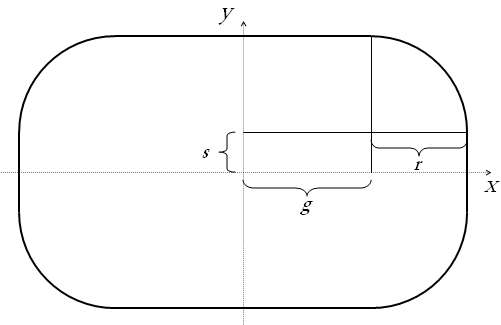
\includegraphics[width=450px]{Introduction/tolerance.jpg}
%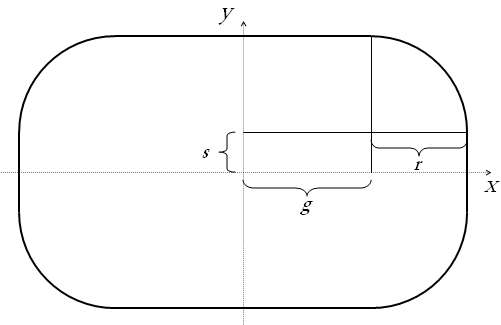
\includegraphics{Introduction/tolerance.jpg align=center width=450}
\\ 
A tolerance can be assigned to each element in a MAD-X sequence as a vector: 
\begin{verbatim}
Syntax: APER_TOL = {r, g, s};

MB : SBEND, L := l.MB, APER_TOL={1.5, 1.1, 0};
\end{verbatim}

\section{APERTURE MODULE}
Computes the n1 values for a piece of machine. Each element is sliced
into thick subelements at given intervals, and the available aperture is
computed at the end of each slice. The computation is based on the last
Twiss table, so it is important to run the
\href{../twiss/twiss.html}{Twiss} and aperture commands on the same
period or sequence, see the aperture example below. Also showed in the
example is how n1 values can be \href{../plot/plot.html}{plotted}.   

{\bf Warning: the aperture command makes the assumption of ultrarelativistic
particles (v\(\approx\)c).}

The minimum n1 for each element is written to the last Twiss table, to
allow for \href{../match/match.html}{matching} by aperture.   
	
\begin{verbatim}
Aperture,
    file=filename, halofile=filename, pipefile=filename, range=range,
    exn=real, eyn=real, dqf=real, betaqfx=real, dp=real, dparx=real, dpary=real,
    cor=real, bbeat=real, nco=integer, halo={real,real,real,real},
    interval=real, spec=real, notsimple=logical, trueprofile=filename,
    offsetelem=filename;
\end{verbatim} 
where the parameters have the following meaning: 
\begin{itemize}
   \item file: Output file with aperture table. Default = none 
   \item halofile: Input file with halo polygon coordinates. Will
     suppress  an eventual halo parameter. Default = none  
   \item range: \href{../Introduction/ranges.html}{Range} given by
     elements. Default = \#s/\#e  
   \item exn: Normalised horizontal emittance. Default = 3.75*e-6  
   \item eyn: Normalised vertical emittance. Default = 3.75*e-6 
   \item dqf: Peak linear dispersion [m]. Default = 2.086 
   \item betaqfx: Beta x in standard qf [m]. Default = 170.25 
   \item dp: Bucket edge at the current beam energy. Default = 0.0015 
   \item dparx: Fractional horizontal parasitic dispersion. Default = 0.273 
   \item dpary: Fractional vertical parasitic dispersion. Default = 0.273 
   \item cor: Maximum radial closed orbit uncertainty [m]. Default = 0.004 
   \item bbeat: Beta beating coefficient applying to beam size. Default = 1.1 
   \item nco: Number of azimuth for radial scan. Default = 5 
   \item halo: Halo parameters: \{n, r, h, v\}. n is the radius of the
     primary halo,  r is the radial part of the secondary halo, h and v
     is the horizontal and  vertical cuts in the secondary halo. Default
     = \{6, 8.4, 7.3, 7.3\}  
   \item interval: Approximate length in meters between
     measurements. Actual value:  nslice = nodelength/interval, nslice
     is rounded down to closest integer,  interval =
     nodelength/nslice. Default = 1.0  
   \item spec: Aperture spec, for plotting only. Gives the spec line in
     the plot. Default = 0.0  
   \item notsimple: Use only if one or more beamscreens in the range are
     considered not to  be a "simply connex". Since all MAD-X apertypes
     are simply connex, this is only possible  if an input file with
     beam screen coordinates are given. See below for a graphical
     example. Default = false.  
   \item trueprofile: A file containing a list of magnets, and for each
     magnet a list of horizontal and vertical deviations from the ideal
     magnet axis. These values may come from measurements done on the
     magnet. See below for example. Default = none.  
   \item offsetelem: A file containing a reference point in the machine,
     and a list of magnets with their offsets from this point described
     as a parabola. See below for example. Default = none.  
\end{itemize}


\subsection{Not simply connex beam pipes} 
Methodically, the algorithm for finding the largest possible halo is
fairly simple. The distance from halo centre to the first apex (i = 0)
in the halo is calculated (l\_i), and the equation for a line going
through these points is derived. This line is then compared with all
lines making the pipe polygon to find their respective intersection
coordinates. The distance h\_i between halo centre and intersection are
then divided by l\_i, to find the maximal ratio of enlargement, as seen
below. This procedure is then repeated for all apexes i in the halo
polygon, and the smallest ratio  of all apexes is the maximal
enlargement ratio for this halo to just touch the pipe at this
particular longitudinal position. 
\\
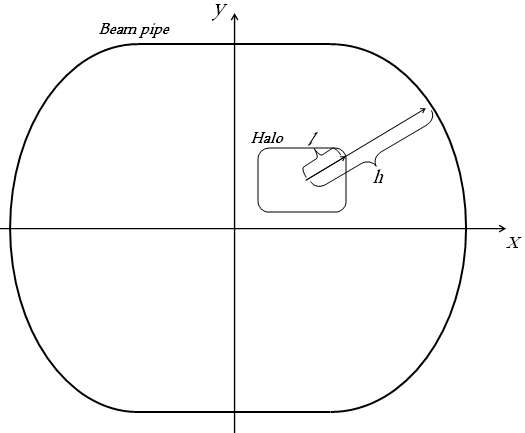
\includegraphics[width=420px]{Introduction/notsimple0.jpg}
%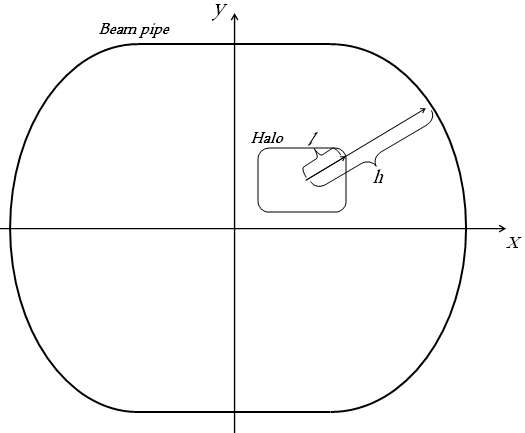
\includegraphics{notsimple0.jpg align=center width=420}
\\  
There is one complication to this solution; polygons which are not
simple connexes. (Geometrical definition of ``simply connex'': A figure
in which any two points can be connected by a line segment, with all
points on the segment inside the figure.) The figure below shows what
happens when a beam pipe polygon is not a simple connex. The halo is
expanded in such a way that it overlaps the external polygon in the area
where the latter is dented inwards. 
\\
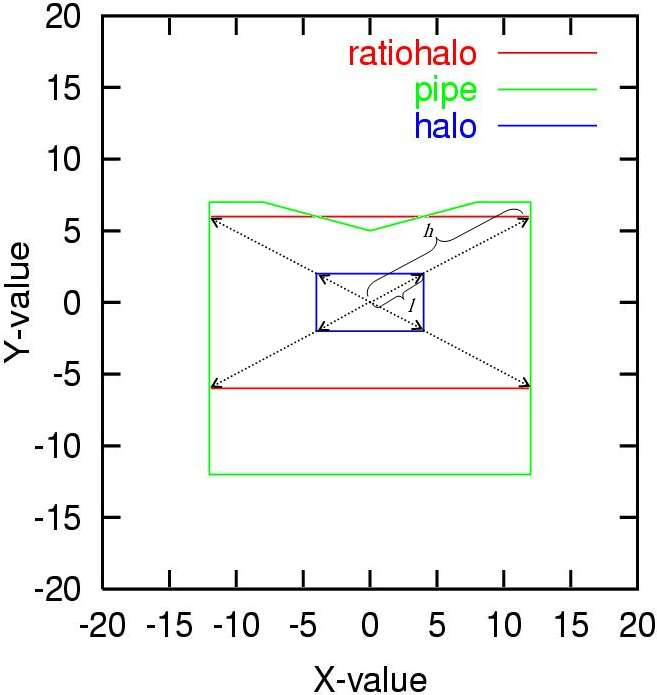
\includegraphics[width=420px]{Introduction/notsimple1.jpg}
%%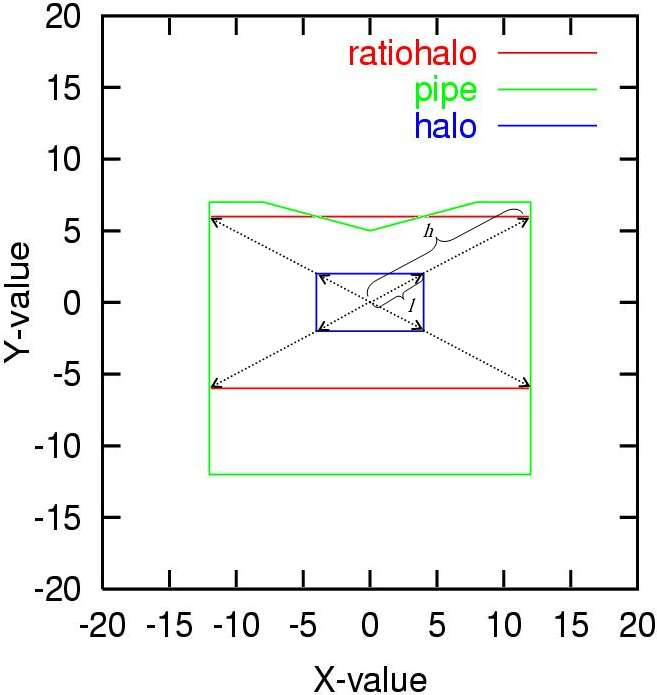
\includegraphics{notsimple1.jpg align=center width=420}
\\  
To make the module able to treat all kinds of polygons,
\textit{notsimple} must be activated. With this option activated, apexes
are strategically added to the halo polygon wherever the beam pipe
polygon might have an inward dent. This is done by drawing a line from
halo centre to each apex on the pipe polygon. An apex with its
coordinates on the intersection point line-halo is added to a table of
halo polygon apexes. The result is that the halo polygon has a few
``excessive'' points on straight sections, but the algorithm used for
expansion will now never miss a dent in the beam pipe. The use of the
notsimple option significantly increases computation time. 
\\
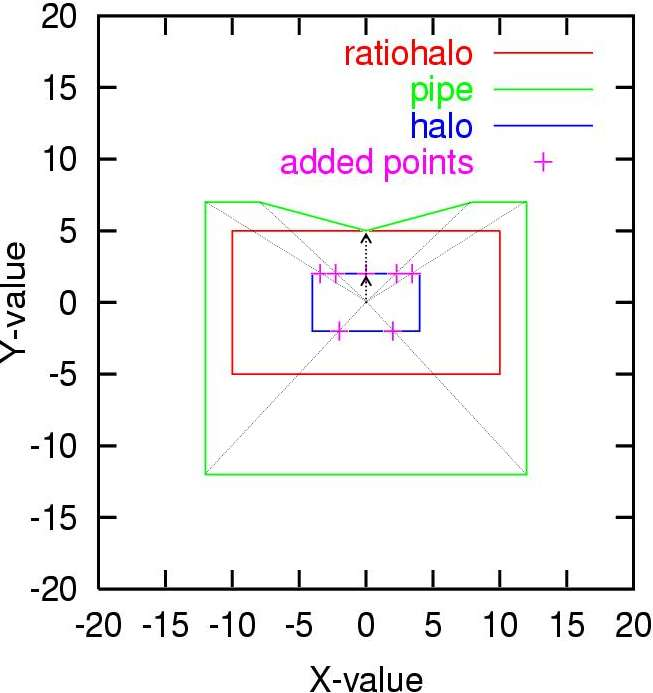
\includegraphics[width=420px]{Introduction/notsimple2.jpg}
%%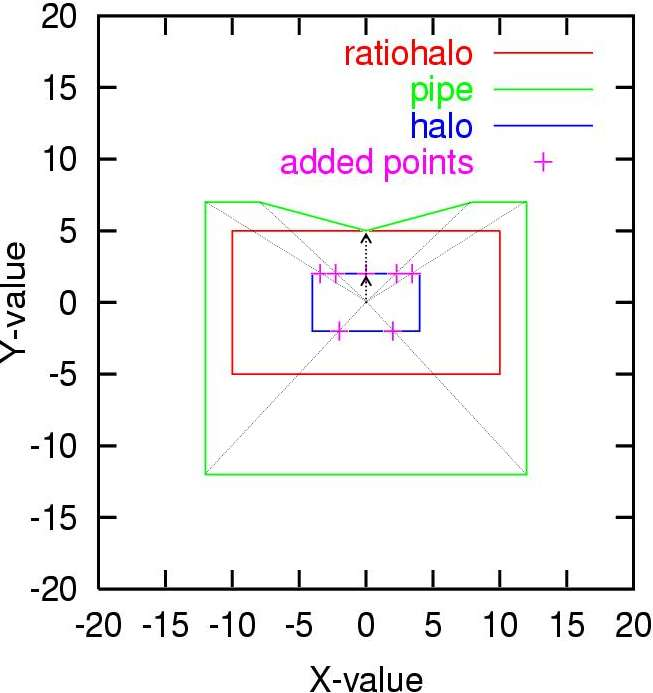
\includegraphics{notsimple2.jpg align=center width=420}
\\

\subsection{Trueprofile file syntax}
This file contains magnet names, and their associated displacements of
the axis for  an arbitrary number of S, where So is the start of the
magnet and Sn the end. The interval between each S must be regular, and
X and Y  must be given in meters. The magnet name must be identical to
how it appears in the  sequence. The displacements are only valid for
this particular magnet, and cannot be  assigned to a family of
magnets. n1 is calculated for a number of slices determinated by the
number of Si. 
\\
{\bf Layout of file:}
\begin{verbatim}
magnet.name1
So   X   Y
Si   X   Y
Si   X   Y
Sn   X   Y

magnet.name2
So   X   Y
Si   X   Y
Si   X   Y
Sn   X   Y

etc.
\end{verbatim}

{\bf Example of file:}
\begin{verbatim}
!This is the start of the file.
!Comments are made with exclamation marks.

mb.a14r1.b1
0        0.0002        0.000004
7.15     1.4e-5        0.3e-3
14.3     0.0000000032  4e-6

!further comments can of course be added

mq.22r1.b1
0      0.3e-5     1.332e-4
1.033  0.00034    0.3e-9
2.066  0          0.00e-2
3.1    4.232e-4   0.00000003

!This is the end of the file.
\end{verbatim}

\subsection{Offsetelem file syntax}
This file contains coordinates describing how certain elements are
displaced w.r.t. a  given reference point in the machine. It might be
used with elements in insertions, or other special-purpose elements that
has a magnet axis which does not coincide with the reference
trajectory. We operate with two coordinate system, s,x and s,y, where
the reference point is the origin and the actual element axis is
described as a parabola with coefficients A, B and C. For each element
we give two sets of coefficients, one for horizontal displacement and
one for vertical:  
\begin{verbatim}
X_offs(s) = Ax*s^2 + Bx*s + Cx 
\end{verbatim}
and 
\begin{verbatim}
Y_offs(s) = Ay*s^2 + By*s + Cy
\end{verbatim}.
The coordinate systems are in meters. 

{\bf Layout of file: --- FOR MADX VERSION 3.XX AND OLDER ONLY--- }
\begin{verbatim}
reference.point

magnet.name1
Ax   Bx   Cx
Ay   By   Cy

magnet.name2
Ax   Bx   Cx
Ay   By   Cy

etc.
\end{verbatim}

{\bf Example of file:}
\begin{verbatim}
!This is the start of the file.
!First we give a reference point. The origin of the 
!coordinate system will be at the START of this element.

mq.12r1.b1

!Then we give a list of elements and their displacement 
!w.r.t. the reference point.

mcbxa.3l2
0   -2.56545   -3
0   -2.3443666  0

!The next nodes use the same reference point.
!Elements offset w.r.t. another point must be given in another file,
!together with the new reference point.

mcbxa.3r2
0.3323  32.443355 -0.84
0.2522  32.554363 0.0

!This is the end of the file.
\end{verbatim}

{\bf Layout of file: --- FOR MADX VERSION 4.XX ONWARDS : now TFS format --- }\\ 
note that variable names changes with : Ax -\textgreater DDX\_OFF,   Bx
-\textgreater DX\_OFF,  Cx -\textgreater X\_OFF, same for Y The column
S\_IP is useless but mandatory (!). It results from a
misunderstanding. Content is ignored. In a future version, it will be
suppressed (but will not induce an error if present).  

% I aligned below lines by hand, do not touch them
\begin{verbatim}
@ NAME             %06s "OFFSET" 
@ TYPE             %06s "OFFSET" 
@ REFERENCE        %10s "mq.12r1.b1" 
* NAME         S_IP   X_OFF  DX_OFF     DDX_OFF   Y_OFF  DY_OFF      DDY_OFF
"mq.12r1.b1"   0.0   -3.0    -2.56545   0.0       0.0    -2.3443666  0.0
"mcbxa.3r2"    0.0   -0.84   32.443355  0.3323    0.0    32.554363   0.2522

A python script to convert a file from the old V.3.XX 
format to the new V4.xx can be found at :

/afs/cern.ch/eng/lhc/optics/V6.503/aperture/convert_offsets.py

usage : convert_offsets.py filename
\end{verbatim}

As an example we see in the picture below how the horizontal axes of
elements m1 and m2 does not coincide with the reference trajectory.  
\\
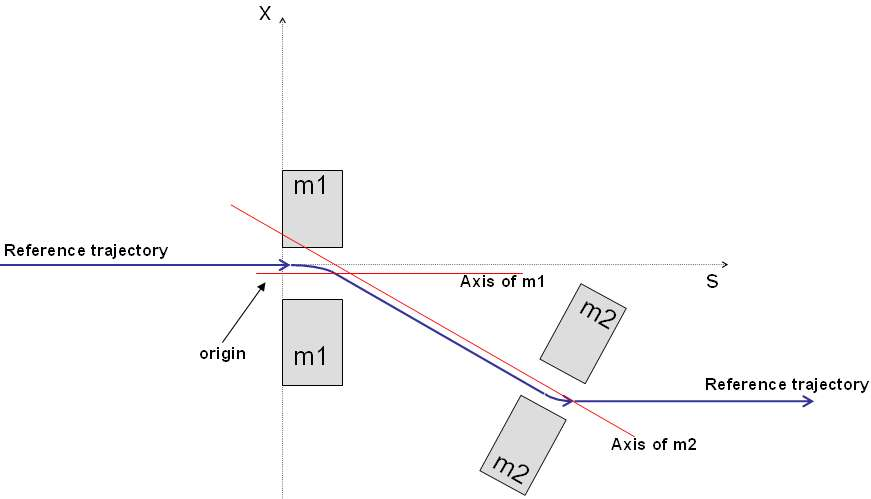
\includegraphics[width=450px]{Introduction/offsetelem.jpg}
%%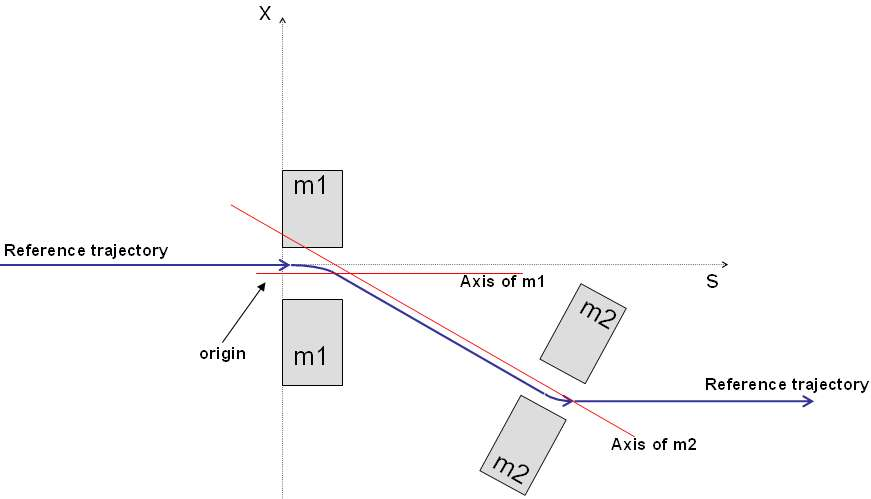
\includegraphics{offsetelem.jpg align=center width=780}
\\ 
The X\_ref(s) and Y\_ref(s) of the reference trajectory are
calculated via an internal call to the
\href{../survey/survey.html}{Survey} module. X\_offs(s) and Y\_offs(s)
are derived from the coefficients given in the file. The resulting  
\begin{verbatim}
X_tot(s) = X_ref(s) - X_offs(s)
\end{verbatim} 
and 
\begin{verbatim}
Y_tot(s) = Y_ref(s) - Y_offs(s)
\end{verbatim} 
are taken into account in the aperture calculations.  


\section{Aperture command example}
The aperture module needs a Twiss table to operate on. It is important
not to USE another period or sequence between the Twiss and aperture
module calls, else aperture looses its table. One can choose the ranges
for Twiss and aperture freely, they need not be the same.  

\begin{verbatim}
use, period=lhcb1;
select, flag=twiss,range=mb.a14r1.b1/mb.a17r1.b1,column=keyword,name,
parent,k0l,k1l,s,betx,bety,n1;
twiss, file=twiss.b1.data, betx=beta.ip1, bety=beta.ip1, x=+x.ip1, 
y=+y.ip1, py=+py.ip1;
plot,haxis=s,vaxis=betx,bety,colour=100;

select, flag=aperture, column=name,n1,x,dy;
aperture, range=mb.b14r1.b1/mb.a17r1.b1, spec=5.235;
plot,table=aperture,noline,vmin=0,vmax=10,haxis=s,vaxis=n1,spec,
on_elem,style=100;
\end{verbatim}

The \href{../Introduction/select.html}{select} command can be  used to choose which columns to print in the output file.  
\\ Column names: name, n1, n1x\_m, n1y\_m, apertype, aper\_1, aper\_2,
aper\_3, aper\_4, rtol, xtol, ytol, s, betx, bety, dx, dy, x, y, on\_ap,
on\_elem, spec  

n1 is the maximum beam size in sigma, while n1x\_m and n1y\_m is the n1 values in si-units in the x- and y-direction. 

aper\_\# means for all apertypes but racetrack:
\\ aper\_1 = half width rectangle
\\ aper\_2 = half heigth rectangle
\\ aper\_3 = half horizontal axis ellipse (or radius if circle)
\\ aper\_4 = half vertical axis ellipse

For racetrack, the aperture parameters will have the same meaning as the tolerances:
\\ aper\_1 and xtol = horizontal displacement of radial part 
\\ aper\_2 and ytol = vertical displacement of radial part 
\\ aper\_3 and rtol = radius 
\\ aper\_4 = not used 

On\_elem indicates whether the node is an element or a drift, and on\_ap
whether it has a valid aperture. The Twiss parameters are the
interpolated  values used for aperture computation.  

When one wants to plot the aperture, the table=aperture parameter is
necessary. The normal line of hardware symbols along the top is not
compatible with the aperture table, so it is best to include
noline. Plot instead the column on\_elem along the vaxis to have a
simple picture of the hardware. Spec can be used for giving a limit
value for n1, to have something to compare with on the plot. This
example  provides a plot,  

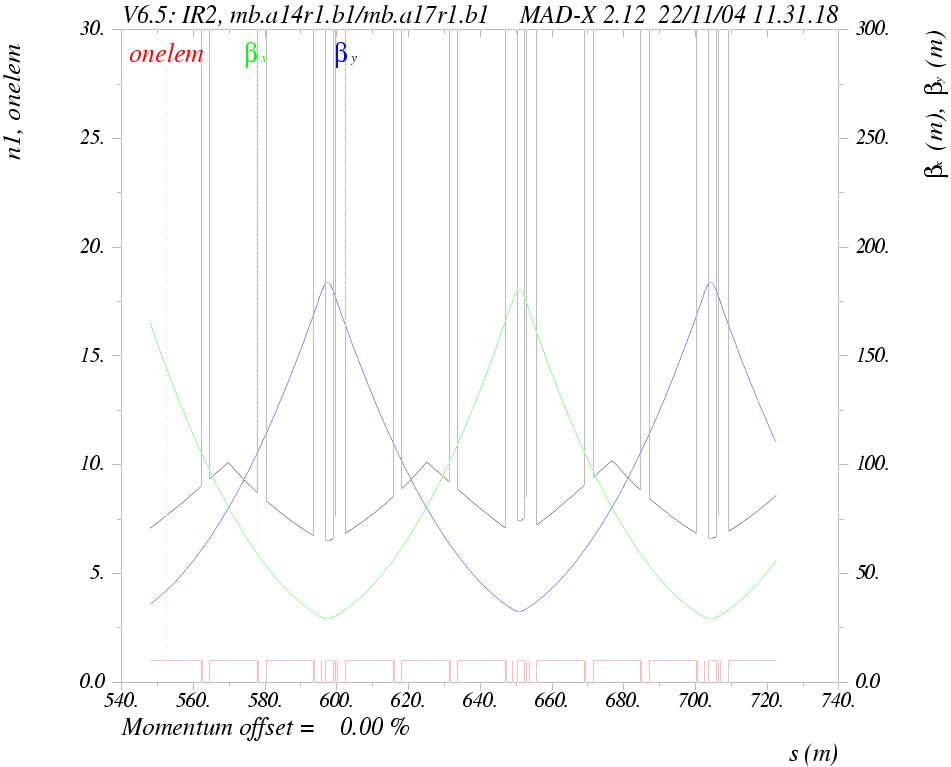
\includegraphics[width=450px]{Introduction/aperexample.jpg}
%%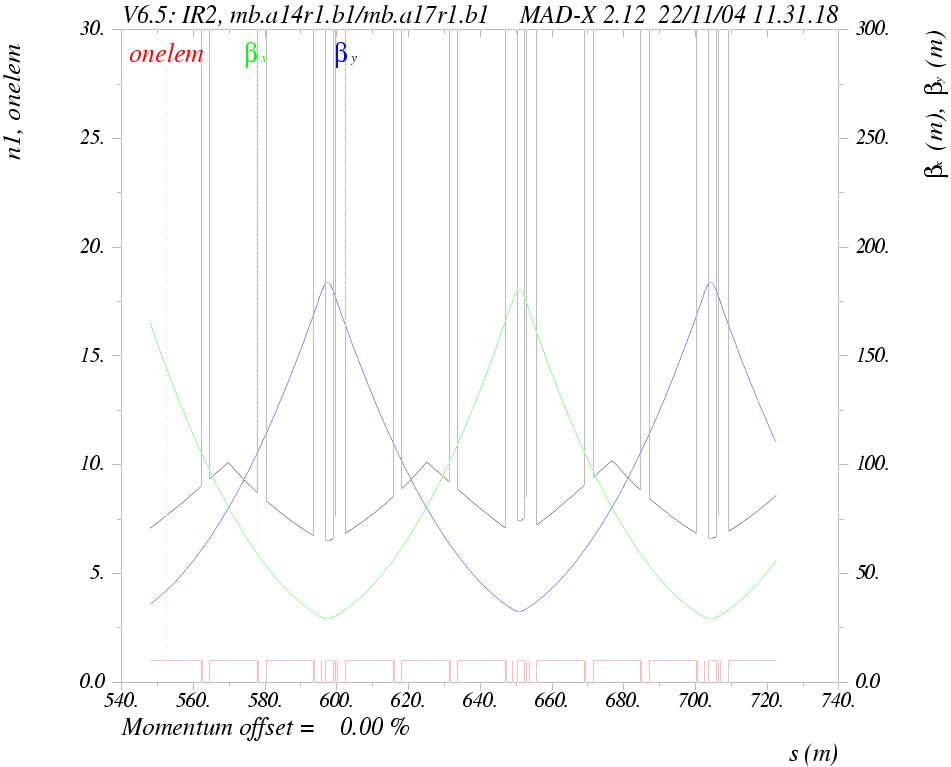
\includegraphics{aperexample.jpg align=center width=740}

where we see the n1, beta functions and the hardware symbolized by on\_elem.    


% Ivar Waarum, 24.02.05  -  Mark Hayes, 19.06.02 

      % APERTURE: defining and calculating apertures 
%%\title{MAKETHIN}
%  Changed by: Helmut Burkhardt,  7-April-2005 
%  Changed by: Helmut Burkhardt, Ghislain Roy -  6-Mai-2014 
 
\chapter{Slicing a sequence into thin lenses}
\label{chap:makethin}

This module takes a sequence with thick elements and creates another one 
with similar functionality but composed of
thin (zero length) element slices or simplified thick slices as required
by \madx tracking or conversion to {\tt SIXTRACK} input format.

\section{MAKETHIN}
\label{sec:makethin}

The slicing is performed by the command: 
\madbox{
MAKETHIN, SEQUENCE=seqname, STYLE=string, MAKEDIPEDGE=logical;
}

The parameters are defined as: 
\begin{madlist}
   \ttitem{SEQUENCE} seqname is the name of the sequence to be
   processed to thin slices. The sequence must be active, i.e. it should
   have been previously loaded with a \hyperref[sec:use]{\tt USE} command.  
   The sequence must use the default positioning of elements ({\tt REFER=centre}).

   \ttitem{STYLE} the slicing style to be used for all elements. \\
   Available slicing styles are: 

   \begin{madlist}
   	\ttitem{TEAPOT} is the default slicing algorithm for all elements 
   	except collimators and is described in \cite{burkhardt2013}. 
   	{\tt TEAPOT} is a clear improvement over the {\tt SIMPLE} algorithm.
   	
   	\ttitem{SIMPLE} produces slices of equal strength and length at equidistant
   	positions.
   	
   	\ttitem{COLLIM} is the default slicing algorithm for collimators. 
   	If only one slice is chosen it is placed in the middle of the old
   	element. If two slices are chosen they are placed at either
   	end. Three slices or more are treated as one slice. 
   	
   	\ttitem{HYBRID} is the previous default algorithm 
   	that was active up to version 5.02.05 when the {\tt STYLE} 
   	attribute was not given; the standard slicing for all
   	elements, except collimators, is {\tt TEAPOT} if the number
   	of slices is less or equal to four, and {\tt SIMPLE} otherwise.
   
   \end{madlist}
   
   \ttitem{MAKEDIPEDGE} is a logical flag to control the generation of
   {\tt DIPEDGE} elements at the start and/or end of bending magnets,
   to conserve edge focusing from pole face angles {\tt E1, E2}
   or extra fields described by {\tt FINT, FINTX}, in the
   process of slicing bending magnets to thin multipole slices.   
   Selection with {\tt THICK=true} will translate a complex thick 
   {\tt RBEND} or {\tt SBEND}, including edge effects, to a simple
   thick {\tt SBEND} with edge focusing transferred to extra 
   {\tt DIPEDGE} elements. \\ 
   (Default:~true)
\end{madlist}

Example:
\madxmp{
! keep translated rbend as thick sbend \\
SELECT, FLAG=makethin, CLASS=rbend, THICK=true;
}

\section{Controlling the number of slices}
\label{sec:numberofslices}

The number of slices can be set individually for elements or groups of
elements using the {\tt SELECT} command
\madxmp{
SELECT, \=FLAG=makethin, \\
        \>RANGE=range, CLASS=class, PATTERN=pattern[,FULL][,CLEAR], \\
        \>THICK=logical, SLICE=integer;
}
where the argument to the attribute {\tt SLICE} stands for the number of
slices for the selected elements. The default is one slice and
{\tt THICK=false} for all elements, i.e. conversion of all thick
elements to a single thin slice positioned at the centre of the original
thick element.

Note that {\tt THICK=true} only applies to dipole or quadrupole magnetic
elements and is ignored otherwise.

{\tt MAKETHIN} allows for thick quadrupole slicing with insertion of
thin {\tt MULTIPOLE} elements between thick slices. 
Positioning is done with markers between
slices, here however with thick slice quadrupole piece filling the whole
length.

{\bf Examples:}
\madxmp{
! slice quadrupoles in three thick slices, insert 2 markers per quadrupole \\
SELECT, FLAG=makethin, CLASS=quadrupole, THICK=true, SLICE=3; \\ 
\\
! thick slicing for quadrupoles named mqxa, insert one marker in the middle \\
SELECT, FLAG=makethin, PATTERN=mqxa$\backslash$., THICK=true, SLICE=2; 
}

Slicing can be turned off for certain elements or classes by specifying
a number of slices $< 1$. Examples: 
\madxmp{
! turn off slicing for sextupoles \\
SELECT, FLAG=makethin, CLASS=sextupole, SLICE=0;  \\
\\
! keep elements unchanged with names starting by mbxw \\
SELECT, FLAG=makethin, PATTERN=mbxw$\backslash$., SLICE=0; 
}
This option allows to introduce slicing step by step and monitor the 
resulting changes in optics parameters.

Keep in mind however that subsequent tracking generally requires full
slicing, with possible exception of dipole and quadrupole magnetic elements. 

\section{Choice of options for dipoles}

There are several options that affect the slicing of a sequence. 
Depending whether dipole magnets (\hyperref[sec:bend]{{\tt RBEND} 
or {\tt SBEND}}) are kept as thick elements 
(See \hyperref[sec:select]{\tt SELECT, FLAG=makethin}) and 
whether the \hyperref[sec:makethin]{\tt MAKEDIPEDGE} option 
of {\tt MAKETHIN} is used to generate 
\hyperref[sec:dipedge]{\tt DIPEDGE} elements around these bending magnets, 
the resulting sequence is more adapted to optics calculation or tracking. 
The following table gives an indication of the best choice of options for 
dipole elements 

\begin{table}[ht]
\caption{Best choice of options in {\tt MAKETHIN}}
\vspace{1ex}
\begin{center}
	\begin{tabular}{|l|l|l|}
	\hline
	   & {\tt THICK=false} & {\tt THICK=true}\\
	\hline
	{\tt MAKEDIPEDGE=false} & backward compatibility & thick optics calculations \\
	\hline
	{\tt MAKEDIPEDGE=true} & thin tracking & thick tracking \\
	\hline
	\end{tabular}
	\end{center}
\end{table}

The combination of \hyperref[sec:numberofslices]{\tt THICK=false} 
(dipoles converted to thin lenses) 
and \hyperref[sec:makethin]{\tt MAKEDIPEDGE=false} 
(no \hyperref[sec:dipedge]{\tt DIPEDGE} 
thin elements inserted around the dipoles) results in a lattice with 
Twiss parameters that can differ significantly from those of 
the original sequence. 
This is most obvious with the tune or phase advance parameters 
that are generally differing by a significant amount (see first 
hint below). This combination is however useful for backward compatibility 
with previous versions of {\tt MAKETHIN} before 
\hyperref[sec:dipedge]{\tt DIPEDGE} elements were
implemented. 

The combination of \hyperref[sec:numberofslices]{\tt THICK=true} 
(dipoles are kept as thick elements and not converted to thin lenses) 
and \hyperref[sec:makethin]{\tt MAKEDIPEDGE=false} 
(\hyperref[sec:dipedge]{\tt DIPEDGE} thin elements 
are not inserted around the thick dipoles to replace the edge effects 
that stay with the bends themselves) 
results in a lattice with \hyperref[chap:twiss]{\tt TWISS} parameters 
very comparable to those of the original sequence. The dipoles are still 
thick elements, eventually sliced, with proper edge effects up to second 
order, although non-symplectic.
This is the best combination for optics studies without particle tracking, 
e.g. with \hyperref[chap:twiss]{\tt TWISS}. 

The combination of \hyperref[sec:numberofslices]{\tt THICK=false} for dipoles 
and \hyperref[sec:makethin]{\tt MAKEDIPEDGE=true} 
transforms the original dipoles into one or several thin slices without 
any edge effect, surrounded by a pair of \hyperref[sec:dipedge]{\tt DIPEDGE} 
elements at the original location of dipole entrance and exit. 
Note however that these \hyperref[sec:dipedge]{\tt DIPEDGE} elements only 
contain first order effects for the purpose of tracking. 

The combination of \hyperref[sec:numberofslices]{\tt THICK=true} for dipoles 
and \hyperref[sec:makethin]{\tt MAKEDIPEDGE=true} 
conserves the dipoles as thick element dipole bodies only while their associated 
edge effects are transferred to \hyperref[sec:dipedge]{\tt DIPEDGE} elements
that are taken into account at first order only for symplectic tracking.

\section{Additional information}

The generated thin lens sequence has the following properties: 
\begin{itemize}
\item The new sequence has the same name as the original. 
  The original sequence is replaced by the new one in memory. 
  If the original sequence is needed for further processing in \madx, 
  it should be reloaded.
\item The algorithm also processes any sub-sequence inserted in the main
  sequence. These sub-sequences are also given the same names as the
  original ones. 
\item Any element transformed into a single thin lens element has the
  same name as the original. 
\item If an element is sliced into more than one slice, the individual
  slices have the same basename as the original element plus a suffix 
  {\tt ..1}, {\tt ..2}, etc. and a marker, with the name of the original
  element, is placed at the location of the center of the original element.
\end{itemize}


{\bf Hints}
\begin{enumerate}
\item Compare the main optics parameters like tunes before and after slicing
  with {\tt MAKETHIN}. Rematch tunes and chromaticity as necessary after
  {\tt MAKETHIN}. 

\item In tests, turn off slicing for some of the main element classes to
  identify the main sources of changes. 

\item For sextupoles and octupoles, a single slice should always be sufficient.

\item Increase the number of slices for critical elements like mini-beta
  quadrupoles. Even there, more than four slices should rarely be
  required. 

\item In case of problems or doubts, consider to
  {\tt FLATTEN} the sequence before slicing.  

\item See the
  \href{http://madx.web.cern.ch/madx/madX/examples/makethin/}{examples}
  for makethin. \\ 
  See also the presentations on the upgrade of the makethin module:\\
  \href{http://ab-dep-abp.web.cern.ch/ab-dep-abp/LCU/LCU_meetings/2012/20120918/LCU_makethin_2012_09_18.pdf}{LCU\_makethin\_2012\_09\_18.pdf}, and \\
  \href{http://ab-dep-abp.web.cern.ch/ab-dep-abp/LCU/LCU_meetings/2013/20130419/LCU_makethin_2013_04_19.pdf}{LCU\_makethin\_2013\_04\_19.pdf}. \\ 
  TEAPOT is documented in \href{http://accelconf.web.cern.ch/AccelConf/IPAC2013/papers/mopwo027.pdf}{IPAC'13 MOPWO027}

\end{enumerate}

%%%%%%%%
      % MAKETHIN: Conversion to Thin Lens
%%\title{Error Definitions}

\chapter{Error Definitions}  
\label{chap:error}
This chapter describes the commands which provide error assignment and
output of errors assigned to elements. It is possible to assign
alignment errors and field errors to single beam elements or to ranges
or classes of beam elements.  

Elements, classes or ranges of elements are selected by the
\href{../Introduction/select.html}{SELECT} command.  

ATTENTION: since errors can only be assigned to machine elements, it is
necessary to  \href{../control/seqedit.html#flatten}{FLATTEN} a sequence
if it includes other sequences.  

Errors can be specified both with a constant or random values. Error
definitions consist of four types of statements listed below. They may
be entered after having selected a beam line by means of a
\href{../control/general.html#use}{USE} command.  

WARNING: any further \href{../control/general.html#use}{USE} command
will destroy the assigned errors. Use the
\href{../error/error_save.html}{ESAVE} option to save and reload errors.  

%\begin{itemize}
%	\item \href{error_align.html}{EALIGN: Define Misalignments}
%	\item \href{error_field.html}{Field Errors}
%\begin{itemize}
%	\item \href{error_field.html#efcomp}{EFCOMP: Components}
%\end{itemize}
%	\item \href{error_option.html}{EOPTION: Set Error Options}
%	\item \href{error_print.html}{EPRINT: List Machine Imperfections}
%	\item \href{error_save.html}{ESAVE: Save Machine Imperfections and read back from file}
%\end{itemize}

%\href{http://consult.cern.ch/xwho/people/1808}{Werner Herr} 18.6.2002 

% add other files to the end of this file

%%\title{EALIGN}
%  Changed by: Hans Grote, 13-Sep-2000 

%  Changed by: Werner Herr, 19-Jun-2002 

%  Changed by: Hans Grote, 19-Jun-2002 

%  Changed by: Werner Herr, 24-Jul-2002 

%  Changed by: Werner Herr, 02-Sep-2002 

%  Changed by: Hans Grote, 25-Sep-2002 

%%\usepackage{hyperref}
% commands generated by html2latex


%%\begin{document}

\section{EALIGN: Define Misalignments}  Alignment errors are defined by the EALIGN command. The misalignments refer to the \href{../Introduction/local_system.html}{local reference system} for a perfectly aligned machine. Possible misalignments are displacements along the three coordinate axes, and rotations about the coordinate axes. Alignment errors can be assigned to all beam elements except drift spaces. The effect of misalignments is treated in a linear approximation. A \href{read HREF=../Introduction/monitors.html}{Beam position monitor} can be given read errors in both horizontal and vertical planes. Monitor errors (MREX, MREY, MSCALX and MSCALY) are ignored for all other elements. Each new EALIGN statement replaces the misalignment errors for all elements in its range, unless EOPTION,ADD=TRUE has been entered. 

 Alignment errors are defined by the statement 
\begin{verbatim}

SELECT,FLAG=ERROR,RANGE=range,CLASS=name,PATTERN=string;
EALIGN, DX=real,DY=real,DS=real, 
        DPHI=real,DTHETA=real,DPSI=real, 
        MREX=real,MREY=real,
        MSCALX=real,MSCALY=real,
        AREX=real,AREY=real;
\end{verbatim} and elements are now selected by the \href{../Introduction/select.html}{SELECT} command. The attributes are: 

DX: The misalignment in the \textit{x}-direction for the entry of the beam element (default: 0 m). 
\\ DX$>$0 displaces the element in the positive \textit{x}-direction 

DY: The misalignment in the \textit{y}-direction for the entry of the beam element (default: 0 m). 
\\ DY$>$0 displaces the element in the positive \textit{y}-direction 

DS: The misalignment in the \textit{s}-direction for the entry of the beam element (default: 0 m). 
\\ DS$>$0 displaces the element in the positive \textit{s}-direction 

DPHI: The rotation around the \textit{x}-axis. 
\\ A positive angle gives a greater \textit{x}-coordinate for the exit than for the entry (default: 0 rad). 

DTHETA: The rotation around the \textit{y}-axis according to the right hand rule (default: 0 rad). 

DPSI: The rotation around the \textit{s}-axis according to the right hand rule (default: 0 rad). 

MREX: The horizontal read error for a monitor. This is ignored if the element is not a monitor 
\\ If MREX$>$0 the reading for \textit{x} is too high (default: 0 m). 

MREY: The vertical read error for a monitor. This is ignored if the element is not a monitor 
\\ If MREY$>$0, the reading for \textit{y} is too high (default: 0 m). 

AREX: The misalignment in the \textit{x}-direction for the entry of an aperture limit (default: 0 m). 
\\ AREX$>$0 displaces the element in the positive \textit{x}-direction 

AREY: The misalignment in the \textit{y}-direction for the entry of an aperture limit (default: 0 m). 
\\ AREY$>$0 displaces the element in the positive \textit{y}-direction 

MSCALX: The relative horizontal scaling error for a monitor. This is ignored if the element is not a monitor. 
\\ If MSCALX$>$0 the reading for \textit{x} is too high (default: 0). A value of 0.5 implies the actual reading is multiplied by 1.5. 

MSCALY: The relative vertical scaling error for a monitor. This is ignored if the element is not a monitor.  
\\ If MSCALY$>$0 the reading for \textit{y} is too high (default: 0). A value of -0.3 implies the actual reading is multiplied by 0.7. 
\\
\\
\\ Example: 
\begin{verbatim}

SELECT,FLAG=ERROR,CLASS=MQ;                  
EALIGN,DX=0.002,DY=0.0004*RANF(),DPHI=0.0002*GAUSS();
\end{verbatim} Assigns alignment errors to all elements of class MQ.           
\\
\begin{verbatim}

SELECT,FLAG=ERROR,PATTERN="QF.*";            
EALIGN,DX=0.001*TGAUSS(2.5),DY=0.0001*RANF();
\end{verbatim} Assigns alignment errors to all elements starting with "QF". TGAUSS(2.5) means a Gaussian distribution cut at 2.5 sigma. 
\\

%\href{xsdisp}{
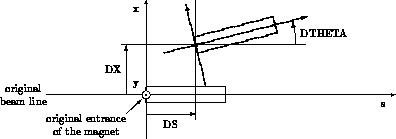
\includegraphics{figures/xs_align.png}

\textbf{Figure 1:} Example of Misplacement in the (\textit{x, s})-plane. 

%\href{xydisp}{
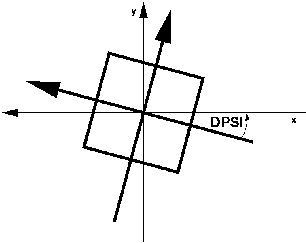
\includegraphics{error/dpsi.png}

\textbf{Figure 2:} Example of Misplacement in the (\textit{x, y})-plane. 

%\href{ysdisp}{
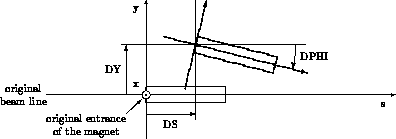
\includegraphics{figures/ys_align.png}

\textbf{Figure 3:} Example of Misplacement in the (\textit{y, s})-plane. 

%\href{monitor}{
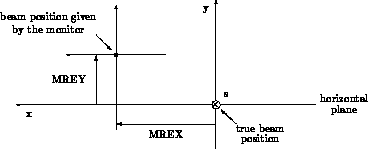
\includegraphics{figures/monitor_read.png}

\textbf{Figure 4:} Example of Read Errors in a monitor 
\\
\\
\\
\\\href{http://consult.cern.ch/xwho/people/1808}{Last updated:} 02.9.2002 \\\href{http://consult.cern.ch/xwho/people/1808}{Werner Herr} 18.6.2002 

%%\end{document}

%%\title{Field Errors}
%  Changed by: Hans Grote, 19-Jun-2002 

\section{Field Errors}
Field errors can be entered as relative or absolute errors. Different
multipole components can be specified with different kinds of errors
(relative or absolute). Relations between absolute and relative field
errors are listed below.  

In MAD8 two commands were used for that purpose: EFIELD and EFCOMP. Only
EFCOMP was implemented in MAD-X since it provides the full functionality
of EFIELD and there was no need for duplication.  

All field errors are specified as the integrated value
int(\textit{K*ds}) of the \href{../Introduction/sign_convent.html}{field
  components} along the magnet axis in m$^{-i}$. There is no provision
to specify a global relative excitation error affecting all field
components in a combined function magnet. Such an error may only be
entered by defining the same relative error for all field components.  

Field errors can be specified for all magnetic elements by the statement  

\begin{verbatim}
SELECT, FLAG = ERROR, RANGE = range, CLASS = name, PATTERN = string;
EFCOMP, ORDER := integer, RADIUS := real,
        DKN  := {dkn(0), dkn(1), dkn(2),...},
        DKS  := {dks(0), dks(1), dks(2),...},
        DKNR := {dknr(0),dknr(1),dknr(2),...},
        DKSR := {dksr(0),dksr(1),dksr(2),...};
\end{verbatim}
and elements are now selected by the
\href{../Introduction/select.html}{SELECT} command. Each new
\href{efcomp}{EFCOMP} statement replaces the field errors for all
elements in its range (s). Any old field errors present in the range are
discarded or incremented depending on the setting of
\href{error_option.html}{EOPTION,ADD}. EFCOMP defines them in terms of
relative or absolute components.  

The attributes are: 
\begin{itemize}
\item ORDER: If relative errors are entered for multipoles, this defines
  the order of the base component to which the relative  errors
  refer. This reference strength \textit{k$_ref$} always refers to the
  normal component. To use a skew component as the reference the
  reference radius should be specified as a negative number. The default
  is zero.  \\
  Please note that this implies to specify \textit{k$_0$} to assign
  relative field errors to a bending magnet since \textit{k$_0$} is used
  for the normalization and NOT the ANGLE.  

\item RADIUS: Radius \textit{R} were dknr(i) or dksr(i) are specified
  for 0...i...20 (default 1 m). This attribute is required if dknr(i) or
  dksr(i) are specified. If \textit{R} is negativ, the skew component is
  used for the reference strength.  

\item DKN(i): Absolute error for the normal multipole strength with
  (2i+2) poles (default: 0  m$^{-i}$).  

\item DKS(i): Absolute error for the skewed multipole strength with
  (2i+2) poles (default: 0  m$^{-i}$).  

\item DKNR(i): Relative error for the normal multipole strength with
  (2i+2) poles (default: 0  m$^{-i}$).  

\item DKSR(i): Relative error for the skewed multipole strength with
  (2i+2) poles (default: 0  m$^{-i}$).  
\end{itemize}


\subsection{Time memory effects:}

The relative errors can be corrected for possible time memory effects. A
correction term is computed and added to the relative error. 

The correction term is parametrized as a 3rd order polynomial in the
reference strength \textit{k$_ref$} according to:  

%\begin{verbatim}
\[ \Delta = \sum (c_i * \textit{k}^{i}_{ref})            i = 0...3\]
%\end{verbatim}
The coefficients c$_i$ for the polynominal must be supplied in the
command.  

Two additional parameters and options are required: 

HYSTER: if it is set to 1 applies the correction term derived from the
reference strength and the coefficients.  

HCOEFFN and HCOEFFS: coefficients (normal and skew) for the computation
of the correction term. The 4 coefficients are specified in increasing
order, starting with the 0th order. Each group of four coefficients is
valid for one order of the field errors. Trailing zeros can be omitted,
preceding zeros must be given.  

\subsection{Examples} 

Example 1 (assign relative errors to quadrupoles); 
\begin{verbatim}
select, flag = error, pattern = "q.*";
efcomp, order := 1, radius := 0.010,
dknr := {0, 4e-1, 1e-1, 2e-3, 0, 0, 0, 0, 0, 0, 0, 0, 0, 0, 0, 0, 0, 0, 0, 0},
dksr := {0, 4e-1, 1e-1, 2e-3, 0, 0, 0, 0, 0, 0, 0, 0, 0, 0, 0, 0, 0, 0, 0, 0};
\end{verbatim}

Example 2 (add time memory effect to relative errors): 
\begin{verbatim}
select, flag = error, pattern = "^q.*";
efcomp, order = 1, radius = 0.020, hyster = 1,
hcoeffn := {0.000, 0.000, 0.000, 0.000,   // coefficients multipole order 0
            0.001, 0.000, 0.000, 0.000,   // coefficients multipole order 1
            0.000, 0.000, 0.002, 0.000},  // coefficients multipole order 2
dknr := {0, 1e-2, 2e-4, 4e-5, 1e-5, 0, 0, 0, 0, 0, 0, 0, 0, 0, 0, 0, 0, 0, 0, 0},
dksr := {0, 1e-2, 2e-4, 4e-5, 1e-5, 0, 0, 0, 0, 0, 0, 0, 0, 0, 0, 0, 0, 0, 0, 0};
\end{verbatim}

See also: \href{../Introduction/expression.html#random}{Random values}
and \href{../Introduction/expression.html#defer}{deferred expressions}.  

%\href{http://consult.cern.ch/xwho/people/1808}{Werner Herr}  6.12.2004 

%%\title{EOPTION}
%  Changed by: Hans Grote, 13-Sep-2000 

%  Changed by: Werner Herr, 19-Jun-2002 

%%\usepackage{hyperref}
% commands generated by html2latex


%%\begin{document}

\section{EOPTION: Set Error Options}  The random generator for MAD is taken from \href{../Introduction/bibliography.html#knuth}{[Knuth]}. The error option command specifies different seeds for random values: 
\begin{verbatim}

EOPTION,SEED=real,ADD=logical;
\end{verbatim}
\begin{itemize}
	\item SEED: Selects a particular sequence of random values. A SEED value is an integer in the range [0...999999999] (default: 123456789). SEED alone continues with the current sequence See also: \href{../Introduction/expression.html#random}{Random values}. SEED may be an expression. 
	\item ADD: If this logical flag is set, an EALIGN or EFCOMP, causes the errors to be added on top of existing ones. If it is not set, new errors overwrite any previous definitions. The default value is TRUE if it is omitted in the EOPTION command. The default value is false if no EOPTION command is used. 
\\Please note a recent modification: the default value for the ADD option is only applied as long as the ADD option has not been set explicitly.
\\ Once it was set with EOPTION, it is NOT reset to the default when       the ADD option is omitted in subsequent calls to EOPTION. 
\end{itemize} Example: 
\begin{verbatim}

EOPTION,SEED=987456321;
\end{verbatim}\href{http://consult.cern.ch/xwho/people/1808}{Werner Herr} 18.6.2002 

%%\end{document}

%%\title{EPRINT}
%  Changed by: Hans Grote, 13-Sep-2000 

\section{EPRINT: List Machine Imperfections}  
\label{sec:eprint}
This command prints a table of errors assigned to elements. The range
for these elements has to be specified. Field errors are printed as
absolute errors, because all relative errors are transformed to the
corresponding absolute error at definition time. An error print is
requested by the statement  

\begin{verbatim}
SELECT, FLAG=ERROR, RANGE=range, CLASS=name, PATTERN=string;
EPRINT;
\end{verbatim}
and elements are now selected by the
\href{../Introduction/select.html}{SELECT} command.  


A listing for ALL elements, i.e. not only the selected, can be obtained
with the command  
\begin{verbatim}
EPRINT, FULL=TRUE;
\end{verbatim} 
In that case, the SELECT command has no effect.

% \href{http://consult.cern.ch/xwho/people/1808}{Werner Herr} 18.6.2002 

%%\title{ESAVE}
%  Changed by: Hans Grote, 13-Sep-2000 
%  Changed by: Werner Herr, 19-Jun-2002 
%  Changed by: Hans Grote, 30-Sep-2002 

\section{Saving and reloading errors to and from tables and files} 
% ESAVE: Save Machine Imperfections and read back from file}

\subsection{Writing errors to a file}

\begin{verbatim}
ESAVE, FILE=string;
\end{verbatim}

This command saves a table of errors assigned to elements on a file,
using a format which can be read in again to obtain the same
results. This allows dumping the errors and reloading them after a new
USE command. The range for these elements has to be specified. An error
save is requested by the statement  

Example: 
\begin{verbatim}
SELECT, FLAG=ERROR, RANGE=range, CLASS=name, PATTERN=string;
ESAVE, FILE=err.file;
\end{verbatim} 
and elements selected by the  \href{../Introduction/select.html}{SELECT}
command are saved to the file.  


To save the errors of all elements to a file, one can use: 
\begin{verbatim}
SELECT, FLAG = ERROR, FULL;                                    
ESAVE, FILE = err.file;
\end{verbatim}

{\bf Please note: in case of field errors, the absolute errors are
  saved and not relative errors. } 

\subsection{Reading errors from a table or file}

To assign errors from a file is not a priori straightforward. It may be
required to re-assign existing errors after a \textbf{USE} command was
executed (which deletes all errors attached to a sequence).  

Errors stored in the form of an internal table (\textit{errtab}) can  be
directly attached to the appropriate positions in the sequence with the
command:  

\begin{verbatim}
SETERR, TABLE=errtab;
\end{verbatim}
The table \textit{errtab} can be generated internally or from an
external file (\textit{errfile}) with the generic command READMYTABLE.  
 

The command sequence: 
\begin{verbatim}
READMYTABLE, file=errfile, table=errtab;
SETERR, TABLE=errtab;
\end{verbatim}
reads the file \textit{errfile} into the table \textit{errtab} and the
command SETERR attaches the errors to the elements in the active
sequence.  

The file \textit{errfile} can be produced by a preceding ESAVE command
or any other utility. It should follow the format of a file generated
with ESAVE (see example program). 

{\bf Please note:}
\begin{enumerate}
   \item To assign correctly the errors from the file to the elements in
     the sequence, all elements must have individual names, otherwise an
     identification is not possible. Elements in the file not identified
     in the active sequence are ignored.  
   \item Errors are assigned to ALL elements found in the file and the
     FLAG=ERROR is set. Therefore the number of elements selected
     corresponding to a command like:  
     \\ SELECT, FLAG=ERROR,...;
     \\ can be different after the execution of SETERR. 
\end{enumerate}

%\href{http://consult.cern.ch/xwho/people/1808}{Werner Herr} 18.6.2002 


         % EFCOMP, EALIGN: Field and alignment errors
%%%\title{Orbit Correction}
%  Added by: Werner Herr, 01-Oct-2002 
%  Changed by: Werner Herr, 22-Oct-2008 

\chapter{Orbit Correction}  

This chapter describes the commands which can be used to correct the
closed orbit or a trajectory. The distorted orbit is taken from an
internal or external TFS table.  

The purpose of this orbit module is to provide some basic tools to
assess the performance of an orbit correction system of a machine in the
design phase.  

Although some interface is available, it cannot and does not provide the
full functionality expected from a dedicated online orbit correction and
steering program.  

%%\title{CORRECT}
%  Changed by: Hans Grote, 13-Sep-2000 
%  Changed by: Werner Herr, 19-Jun-2002 
%  Changed by: Werner Herr, 02-Sep-2002 
%  Changed by: Werner Herr, 01-Oct-2002 
%  Changed by: Werner Herr, 01-May-2003 
%  Changed by: Werner Herr, 05-April-2004 
%  Changed by: Werner Herr, 01-Dec-2004 
%  Changed by: Werner Herr, 22-Oct-2008 

\section{CORRECT: Orbit Correction}  

The CORRECT statement makes a complete closed orbit  or trajectory
correction using the \textbf{computed} values at the monitors  from the
Twiss table.   

The CORRECT command has the following format (not all possible options
included, some options are valid only for special algorithms):  

\begin{verbatim}
CORRECT, ORBIT=myorbit,MODEL=mymodel,TARGET=mytarget,
         FLAG=ring,MODE=lsq,  
         MONERROR=integer,MONON=real,MONSCALE=real,
         PLANE=x,COND=integer,RESOUT=integer,
         CLIST=file1,MLIST=file2; 
\end{verbatim} 

The command CORRECT is set up with defaults which should allow a
reasonable correction for most cases with a minimum of required options
(see Example 1 below).  

The orbit correction must always be preceded by TWISS commands  which
generate Twiss tables. The most recent Twiss table is assumed to contain
the optical parameters and the distorted orbits. 

The options used in the CORRECT command are: 

\begin{itemize}
   \item FLAG: FLAG can be "ring" or "line", either a circular machine
     or a trajectory is corrected.   
     \\ Default flag is "ring". 

   \item MODE: MODE defines the method to be used for corrections. 
     \\ Available modes are LSQ, MICADO and SVD.  The first performs a
     least squares minimization using all available correctors. The mode
     SVD uses a Singular Value Decomposition to compute a correction
     using all available correctors. The latter can also be used to
     condition the response matrix for the modes LSQ or MICADO (using
     COND=1). It is highly recommended to precede a LSQ correction by a
     SVD conditioning (set COND=1).  
     \\ The mode MICADO is a "best kick" algorithm. Naive use or using
     it with a large number of correctors (see option NCORR) can give
     unexpected results. To avoid the creation of local bumps, it is
     recommended to precede a MICADO correction by a SVD conditioning
     (set COND=1).  
     \\ Default mode is MICADO.            

   \item PLANE: If this attribute is x, only the horizontal correction
     is made; if it is y, only the vertical correction is made. (This
     differs from the MAD8 implementation).  
     \\ Default plane is horizontal. 

   \item COND: When COND is 1, a Singular Value Decomposition is
     performed and  the response matrix CONDitioned to avoid linearly
     dependent correctors. This can be used to avoid creation of
     artificial bumps during a LSQ or MICADO correction (requires some
     computing time).  Please note: this option is not robust since it
     depends on parameters which control the determination of singular
     values and redundant correctors. These can be set with the commands
     SNGVAL and SNGCUT. Both parameters depend on the machine and may
     need adjustment. Default values are adjusted to large machines and
     "reasonable" performance for smaller machines.  
     \\

   \item NCORR: Only used by the MICADO algorithm. Defines the number of
     correctors to be used, unless set to 0 in which case all available
     correctors are used.  
     \\ Default is 0 (all available correctors). 

   \item SNGVAL:  Used to set the threshold for finding singular values
     with the COND command. (Hint: smaller number finds fewer singular
     values).  
     \\ Use with care ! 
     \\ Default is 2.0 

   \item SNGCUT:  Used to set the threshold for finding redundant
     correctors with the COND command. (Hint: larger number finds fewer
     redundant correctors).  
     \\ Use with extreme care ! 
     \\ Default is 50.0 

   \item MONERROR: When MONERROR is 1, the alignment errors on monitors
     assigned  by \href{../error/error_align.html}{EALIGN} MREX and MREY
     are taken into account, otherwise they are ignored.  
     \\ Default is 0. 

   \item MONSCALE: When MONSCALE is 1, the scaling errors on monitors
     assigned  by \href{../error/error_align.html}{EALIGN} MSCALX and
     MSCALY are taken into account, otherwise they are ignored.  
     \\ Default is 0. 

   \item MONON: MONON takes a real number between 0.0 and 1.0. It
     determines the number of available monitors. If the command is
     given, each monitor is considered valid with a probability
     MONON. In the average a fraction (1.0 - MONON) of the monitors will
     be disabled for the correction, i.e. they are considered  not
     existing.  This allows to study the effect of missing monitors.  
     \\ Default is 1.0 (100 \%). 

   \item CORRLIM:  A limit on the maximum corrector strength can be
     given and a WARNING is issued if it is exceeded by one or more
     correctors.  Please note: the strengths computed by the correction
     algorithms are NOT limited, only a warning is printed ! 
     \\ Default is 1.0 mrad. \\
\end{itemize}

Normally the last active table provides the orbit to be
corrected and the model for the correction. This can be overwritten
by the appropriate options. Optionally, these tables can be given
names like in:  TWISS, TABLE=name; (see documentation on TWISS
command). To use these named tables, one of the following optional
parameters must be  used:  

\begin{itemize}
   \item ORBIT: When this parameter is given, the orbit to be corrected
     is taken from a named table. The default is the last (named or
     unnamed) Twiss table.  

   \item MODEL: When this parameter is given, the model for the
     correction is taken from a named Twiss table. The default is the
     last (named or unnamed) Twiss table.  

   \item TARGET: When this parameter is given, the correction is made to
     a named target orbit, pre-computed with a TWISS command. Default is
     correction to the zero orbit.  

   \item EXTERN (default: false): When false, the ORBIT and TARGET table
     are assumed to be computed by MAD with a previous twiss
     command. When set to true, that option allows to use twiss tables
     imported from an external file (with the readmytable command), for
     example to use measured BPM data. In that case, the imported twiss
     table is allowed to contain coordinate data only at the location of
     the monitors.  
\end{itemize}

Example of use of CORRECT to reproduce a measured orbit: 
\begin{verbatim}
! To have a refererence optical model
twiss, table=twiss_ref;

! The bpm.tsv is a reduced Twiss file containing only lines for the BPMs
readmytable, file="bpm.tsv", table="twiss_bpm";

! correct orbit using external measurements
correct, flag=ring, mode=micado, ncorr=5, cond=1 ,plane=x, extern,
         model=twiss_ref, orbit=twiss_ref, target=twiss_bpm, 
         error=1.0e-21;
\end{verbatim}


Two attributes affect the printing of tables and results: 
\begin{itemize}
   \item CLIST=\textbf{file}: Corrector settings (in units of rad)
     before and after correction printed to \textbf{file} 

   \item MLIST=\textbf{file}: Monitor readings (in units of m) before
     and after correction printed to \textbf{file} 

   \item RESOUT: This command outputs the results for all monitors and
     all correctors in a computer readable format if its integer
     argument is larger than 0. The argument is added to the
     output. Useful to analyze runs with loops to produce large
     statistics. 
     \\\textbf{ATTENTION: May produce gigantic outputs for large
       machines.} 
     \\

   \item TWISSUM:  If the argument of twissum is larger than 0, it
     prints maximum orbit and r.m.s. for both planes taken from the
     Twiss summary table in computer readable form. Allows to analyze
     orbits etc. at elements that are not monitors or correctors. The
     argument is added to the output.  Only for output: no correction is
     made, all other commands are ignored.  
\end{itemize}

Obsolete commands or options:
\begin{verbatim}
ITERATE, ITERMAX             /* Done with loop feature in MAD commands */
THREADER, THRTOL, WRORBIT    /* Not part of orbit correction module */
M1LIST, M2LIST               /* Replaced by MLIST */
C1LIST, C2LIST               /* Replaced by CLIST */
GETORBIT, PUTORBIT           /* Replaced by generic TFS access */
GETKICK, PUTKICK             /* Replaced by generic TFS access */
\end{verbatim}

\subsection{EXAMPLES} 

for complete MAD input files see section on examples:

Example 1: correct orbit in horizontal plane, taken from most recent
Twiss table, using default algorithm (MICADO)
\begin{verbatim}
 CORRECT, PLANE = x; 
\end{verbatim}

Example 2: no correction, only output of Twiss summary 
\begin{verbatim}
CORRECT, TWISSUM = 1; 
\end{verbatim}

Example 3: correct orbit in horizontal plane, corrector and monitor
output on table 
\begin{verbatim}
CORRECT, PLANE = x, MODE = lsq, CLIST = corr.out, MLIST = mon.out;   
\end{verbatim}

Example 4: correct orbit in horizontal plane, use alignment and scaling
errors, 15\% of orbit correctors faulty
\begin{verbatim}
CORRECT, PLANE = x, MONERROR = 1, MONSCALE = 1, MONON = 0.85; 
\end{verbatim}

%\href{http://consult.cern.ch/xwho/people/1808}{Last updated:} 22.10.2008 


%%%\title{(De)activate Correctors and Monitors}
%  Changed by: Hans Grote, 13-Sep-2000 
%  Changed by: Werner Herr, 19-Jun-2002 
%  Changed by: Hans Grote, 25-Sep-2002 

\section{Activate/Deactivate Correctors or Monitors}
To provide more flexibility with orbit correction two commands are
provided:  

\begin{verbatim}
USEMONITOR, STATUS=flag, SEQUENCE=sequence, RANGE=range, 
            CLASS=class, PATTERN=regex;

USEKICK,    STATUS=flag, SEQUENCE=sequence, RANGE=range,
            CLASS=class, PATTERN=regex;
\end{verbatim}

The command \href{monitor}{USEMONITOR} activates or deactivates a
selection of \href{../Introduction/monitors.html}{beam position
 monitor}s. This command affects elements of types MONITOR, HMONITOR,
or VMONITOR.    

The command  \href{kick}{USEKICK} activates or deactivates a selection
of \href{../Introduction/kickers.html}{orbit correctors}. This command
affects elements of types KICKER, HKICKER, or VKICKER.   


%% The purpose of the two commands is: 
%% \begin{itemize}
%% 	\item \href{monitor}{USEMONITOR}: Activates or deactivates a
%%           selection of \href{../Introduction/monitors.html}{beam
%%             position monitor}s. This command affects elements of types
%%           MONITOR, HMONITOR, or VMONITOR.  
%% 	\item \href{kick}{USEKICK}: Activates or deactivates a selection
%%           of \href{../Introduction/kickers.html}{orbit correctors}. This
%%           command affects elements of types KICKER, HKICKER, or VKICKER.  
%% \end{itemize} 

Both commands have the same attributes: 
\begin{itemize}
   \item STATUS: If this flag is true (on), the selected elements
     are activated. Active orbit monitor readings will be
     considered, and active correctors can change their strengths
     in subsequent correction commands. Inactive elements will be
     ignored subsequently.  
   \item SEQUENCE: The sequence can be specified, otherwise the
     currect sequence is used for this operation.  
   \item RANGE, CLASS, PATTERN: The usual selection commands are
     used to identify the elements for this operation.  
\end{itemize} 

Example:
\begin{verbatim}
USE,...                                ! set working beam line 
...                                    ! define imperfections 
USEKICK, STATUS = OFF, RANGE = ...;    ! deactivate selected correctors 
USEMONITOR, STATUS = OFF, RANGE = ...; ! deactivate selected monitors   
CORRECT, NCORR = 32;                   ! uses different set of correctors
USEKICK, STATUS = OFF, RANGE = ...;    ! deactivate different set of correctors 
CORRECT, NCORR = 32;                   ! uses different set of correctors
\end{verbatim}

%\href{http://consult.cern.ch/xwho/people/1808}{Werner Herr} 18.6.2002 

%%%\title{COPTION}
%  Changed by: Werner Herr, 26-May-2008 



\section{CSAVE: Write orbit correctior settings to file}
\label{sec:csave}
 This section is under construction, options presently only available in
 MADX development version.  

\section{SETCORR: Set orbit correctior settings}
 This section is under construction, options presently only available in
 MADX development version.  

%\href{http://consult.cern.ch/xwho/people/1808}{Werner Herr} 18.6.2002 

%%%\title{COPTION}
%  Changed by: Werner Herr, 19-Jun-2002 

%%%\usepackage{hyperref}
% commands generated by html2latex


%%%\begin{document}

\section{COPTION: Set Orbit Correction Options}  The random generator for MAD is taken from \href{../Introduction/bibliography.html#knuth}{[Knuth]}. 
\\ In the orbit program monitors can be randomly disabled and 
\\ the correct option command specifies different seeds for random values: 
\begin{verbatim}

COPTION,SEED=integer,PRINT=2      
\end{verbatim}
\begin{itemize}
	\item SEED: Selects a particular sequence of random values. 
\\ A SEED value is an integer in the range [0...999999999] (default: 123456789). 
\\ SEED alone continues with the current sequence 
\\ See also: \href{../Introduction/expression.html#random}{Random values}. 
\\ SEED may be an expression. 
	\item PRINT: This flag can take integer values and controls the printout. 
\\ In general: the higher its value the more printout is produced.  
\\ For PRINT=0 no output is produced. 
\\ The default value is 1 (Correction summary is given). 
\end{itemize} Example: 
\begin{verbatim}

COPTION,SEED=987456321,PRINT=2;
\end{verbatim}\href{http://consult.cern.ch/xwho/people/1808}{Werner Herr} 18.6.2002 

%%%\end{document}
 

%\begin{itemize}
%	\item \href{co_correct.html}{CORRECT:  Correction commands and parameters}
%	\item \href{co_activate.html}{Activate/Deactivate correctors and monitors}
%	\item \href{co_corrsave.html}{READ/WRITE corrector settings}
%	\item \href{co_option.html}{COPTION:  Global Correction Options}
%\end{itemize}

%\href{http://consult.cern.ch/xwho/people/1808}{Werner Herr} 22.10.2008 

% add other files to the end of this file

      % CORRECT: Orbit correction
%%\title{SODD}
%  Changed by: E. T. d'Amico, 8-Sep-2004 

%%\usepackage{hyperref}
% commands generated by html2latex


%%\begin{document}
%%\begin{center}
 %%EUROPEAN ORGANIZATION FOR NUCLEAR RESEARCH 
%%\includegraphics{http://cern.ch/madx/icons/mx7_25.gif}

\subsection{SODD}
%%\end{center}

 This command will execute the Second Order Detuning and Distortion as described in the paper of J. Bengtsson and J. Irwin  "Analytical Calculation of Smear and Tune Shift " (SSC-232, February 1990), on the beam line defined by the last USE command followed by a TWISS command. It is based on the stand-alone program written by Frank Schmidt in November 1998 - January 1999 who also extended the analytical computation to the second order distortion (cfr. Beam Physics Note 60 F. Schmidt "SODD: A physics Guide").  It consists of three parts: 


%	\item 

\paragraph{Subroutine detune (launched by the attribute detune)} It calculates the detuning function terms in first and second order in the strength of the multipoles. If the attribute print\_at\_end has been set, the following two files  (and the corresponding madx tables) are created : 

\textit{detune\_1\_end} containing five columns : 

 1) 'multipole order', 2) '(hor., ver. plane => (1/2)',  3) 'hor. or ver. detuning', 4) 'order of horizontal invariant', 5) 'order of vertical invariant'. 


\textit{detune\_2\_end}  containing five columns : 

 1) 'first multipole order', 2) 'second multipole order',  3) 'horizontal detuning', 4) 'order of horizontal invariant', 5)'order of vertical invariant'.  
 If the attribute print\_all has been set, the following two files  (and the corresponding madx tables) are created : 

\textit{detune\_1\_all}  containing  five columns :  

 1) 'multipole order', 2) '(hor., ver. plane => (1/2)',  3) 'hor. or ver. detuning', 4) 'order of horizontal invariant', 5)'order of vertical invariant'. 
 
\textit{detune\_2\_all}  containing five columns :  

 1) 'first multipole order', 2) 'second multipole order',  3) 'horizontal detuning', 4) 'order of horizontal invariant', 5) 'order of vertical invariant'. 



%	\item 

\paragraph{Subroutine distort1 (launched by the attribute distort1)}  It calculates the distortion function and the Hamiltonian terms in first order in the strength of the multipoles. If the attribute print\_at\_end has been set, the two files  (and the corresponding madx tables) are created : 

\textit{distort\_1\_F\_end} containing eight columns : 

 1) 'multipole order', 2) 'cosine part of distortion', 3) 'sine part of distortion', 4) 'amplitude of distortion', 5) 'j', 6) 'k', 7) 'l', 8) 'm'. 

\textit{distort\_1\_H\_end}  containing eight columns : 

 1) 'multipole order', 2) 'cosine part of Hamiltonian', 3) 'sine part of Hamiltonian', 4) 'amplitude of Hamiltonian', 5) 'j', 6) 'k', 7) 'l', 8) 'm'.  
 If the attribute print\_all has been set, the following two files  (and the corresponding madx tables) are created : 

\textit{distort\_1\_F\_all} containing eleven columns :  

 1) 'multipole order', 2) 'appearance number in position range', 3) 'number of resonance', 4) 'position', 5) 'cosine part of distortion', 6) 'sine part of distortion', 7) 'amplitude of distortion', 8) 'j', 9) 'k', 10) 'l', 11) 'm'. 

\textit{distort\_1\_H\_all}  containing eleven columns : 

 1) 'multipole order', 2) 'appearance number in position range, 3) 'number of resonance', 4) 'position', 5) 'cosine part of Hamiltonian', 6) 'sine part of Hamiltonian', 7) 'amplitude of Hamiltonian', 8) 'j', 9) 'k', 10) 'l', 11) 'm'.  



%	\item 

\paragraph{Subroutine distort2 (launched by the attribute distort2)}  It calculates the distortion function and Hamiltonian terms in second order in the strength of the multipoles. If the attribute print\_at\_end has been set, the following two files  (and the corresponding madx tables) are created : 

\textit{distort\_2\_F\_end} containing nine columns : 

 1) 'first multipole order',2) 'second multipole order',  3) 'cosine part of distortion', 4) 'sine part of distortion', 5) 'amplitude of distortion', 6) 'j', 7) 'k', 8) 'l', 9) 'm'. 
 
\textit{distort\_2\_H\_end}  containing nine columns :  

 1) 'first multipole order', 2) 'second multipole order',  3) 'cosine part of Hamiltonian', 4) 'sine part of Hamiltonian', 5) 'amplitude of Hamiltonian', 6) 'j', 7) 'k', 8) 'l', 9) 'm'.  


 N. B. The first row of every file is a header containing the names of the columns. This row is absent in the internal tables. 


%	\item 

\paragraph{\href{sodd}{SODD}}
\begin{verbatim}

sodd,
detune=logical,
distort1=logical,
distort2=logical,
start_stop = start,stop
multipole_order_range = fist,last
noprint = logical
print_all = logical
print_at_end = logical
nosixtrack  = logical
\end{verbatim} where the parameters have the following meaning: 
\begin{itemize}
	\item detune : logical, default=false. If true, the detune subroutine is executed. 
	\item distort1 : logical, default=false. If true, the distort1 subroutine is executed. 
	\item distort2 : logical, default=false. If true, the distort2 subroutine is executed. 
	\item start\_stop : longitudinal interval of the beam line (in m). start and stop should be given as real numbers. 
	\item multipole\_order\_range : the lowest and the largest multipole order which will be taken in account. first and last should be given as integers. 
	\item noprint : logical, default=false. If true, no file or internal table will be created to keep the results. In this case the attributes print\_all or print\_at\_end have no effect. 
	\item print\_all : logical, default=false. If true, the files and internal tables containing results at each multipole will be generated. 
	\item print\_at\_end : logical, default=false. If true, the files and internal tables containing results at the end of the position range will be generated. 
	\item nosixtrack  : logical, default=false. If true, the input file fc.34 will not be generated internally by invoking the conversion routine of sixtrack and the user should provide it before the execution of the sodd command. 

	\item A more detailed description can be found in  \href{http://cern.ch/madx/doc/ab-note-2004-069}{AB-note-2004-069}\href{http://xwho.web.cern.ch/xwho/people/show/6175}{damico}, September 10, 2004 
\end{itemize}

%%\end{document}
          % SODD: Second Order Detuning 
1-9    *     skip     # head
*      *    rel=1e-10 # global

      % Touschek effect
% original version by:  Nikos Drakos, CBLU, University of Leeds
% * revised and updated by:  Marcus Hennecke, Ross Moore, Herb Swan
% * with significant contributions from:
%   Jens Lippmann, Marek Rouchal, Martin Wilck and others 

%Edited:
% Frank Schmidt 2003-05-23 
% Ghislain Roy 2014-08-07


\chapter{Intra-Beam Scattering}
\label{chap:ibs}

The Intra-Beam Scattering command computes the contribution to emittance
growth rates due to Coulomb scattering of particles within relativistic
beams. The algorithms in this module have been derived from the formalism
presented in 1982 by J.D.~Bjorken and S.K.~Mtingwa
\cite{bjorken-mtingwa1982}, and are also using the expansion of M.~Conte
and M.~Martini \cite{conte-martini1985} developped in 1985, generalized
to the case of nonzero vertical dispersion.  

The present implementation of the IBS module in \madx is described in a
forthcoming note  \cite{antoniou-zimmermann2012}.


The syntax of the \texttt{IBS} command is:
\madbox{
%IBS, TOLERANCE=real, STEPS=integer, FILE=string;
IBS, FILE=string;
}

The \texttt{IBS} command has one attribute:
\begin{madlist}
%  \ttitem{TOLERANCE} ??? (Default:~1.e-7) % declared, never used
%  \ttitem{STEPS} number of steps ??? (Default:~50) % declared, never used
  \ttitem{FILE} outputs the resulting "ibs" table to
  the named file. (Default:~"ibs")
\end{madlist}

The Bjorken-Mtingwa formalism takes into account the variation of the
lattice parameters (beta and dispersion functions) around the
machine and consequently, the knowledge of the optical functions along
the machine is required: \texttt{IBS} should only be called after fully
qualified \texttt{BEAM} command and a \texttt{TWISS} command. 

\textbf{Warning:} Calling \texttt{EMIT} between the \texttt{TWISS} and
\texttt{IBS} commands leads to \texttt{IBS} using wrong beam parameters,
even if the \texttt{BEAM} command is reiterated.

The \texttt{IBS} module does not include a consistent treatment of
linear betatron coupling.   

The intra-beam scattering growth times are given by:
\[
 \frac{1}{\tau_i} \quad = \quad C_i \times \frac{N}{\gamma \epsilon_x
   \epsilon_y \epsilon_s} \qquad (i = x, y, s) 
\]
where $C_i$ accounts for some constants and the integrals for the
scattering functions, N is the number of particles in the bunch,
$\gamma$ is the relativistic factor and $\epsilon_i$ are the normalized
emittances in the horizontal, vertical and longitudinal plane
respectively. These key beam parameters must be specified through the
\texttt{BEAM} command. 

If the \texttt{CENTRE=true} option of \texttt{TWISS} was specified,
the optical functions are calculated by \texttt{TWISS} at the center of 
each element and \texttt{IBS} uses these values for the element. 
If by default \texttt{TWISS} calculated the optical functions at the end
of each element, \texttt{IBS} calculates the values at the center of
each element by performing a linear interpolation between the end values
for the previous element and the end values for the current element.

  
\textbf{Input of the beam parameters:}\\
A number of parameters have to be present in the  \texttt{BEAM} command
in order to run the IBS module: 

\begin{madlist}
  \ttitemn{PARTICLE} This is mandatory but \madx provides default
  value of \texttt{PARTICLE=proton}. For ions, this parameter specifies
  only the name of the ions, and the MASS (approximated to the atomic
  unit number times the unified atomic mass \texttt{UMASS}) and CHARGE must be
  provided as well.

  \ttitemn{NPART} the number of particles (or number of ions).

  \ttitemn{ENERGY} The definition of the energy (total, kinetic, total
  energy of the ions or energy per nucleon) is a difficult one. In the
  present approach, the energy is the \textbf{total} energy of the
  particle. For ions, the expected input is the \textbf{proton
    equivalent} energy, i.e. the total energy a proton would have when
  circulating in the defined machine. As an illustration, in the LHC,
  protons will be injected with an energy of 450 GeV. Consequently, to
  evaluate the growth times for Lead ions at injection in the LHC, one
  has to input \texttt{ENERGY=450*charge}. \\
  An important check for the correctness of the input is the printed value
  of the relativistic factor  $\gamma$. The latter should correspond to:   
  \[
  \gamma_{ion} \quad = \quad \gamma_{proton} \times \frac{charge}{nucleon}
  \]

  \ttitemn{emittances} This part of the input is used to define the
  normalized horizontal, vertical and longitudinal emittances. 
  The required parameters are the \texttt{physical} transverse
  emittances, \texttt{EX} and \texttt{EY}, and the longitudinal
  emittance \texttt{ET}.\\  
  The longitudinal emittance is defined  as the product of the bunch
  length \texttt{SIGT} times the relative energy spread \texttt{SIGE},
  which are therefore required input. \\  
  If only the longitudinal emittance is defined, and \texttt{SIGT}
  and \texttt{SIGE} are omitted, an active RF cavity is also
  necessary in the lattice to infer \texttt{SIGT} and \texttt{SIGE}.

\end{madlist}


\textbf{Example of BEAM input:}\\
A beam of fully stripped Lead ions at the LHC injection energy may be
defined as follows for \texttt{IBS} calculations: 
\madxmp{
nucleon = 208; \\
charge = 82; \\
\\
BEAM, \=PARTICLE= lead, CHARGE= charge, MASS= nucleon*umass, \\
      \>ENERGY= 450*charge, NPART= 1.1E7, BUNCHED, \\
      \>EX= 7.82E-9, EY= 7.82E-9, SIGE= 4.68E-4, SIGT= 0.115;
}


\textbf{Resulting Table and File:} \\
The \texttt{IBS} command produces a table "ibs" containing the following
data for 
each element of the machine: element name, position, optical functions
(beta, alfa, dispersion and derivative) in both transverse planes, as
well as the particular variables \texttt{DELS}, the length difference in
meters between consecutive elements, and \texttt{TXI, TYI} and
\texttt{TLI}, the IBS growth times in the two transverse and
longitudinal planes.  

This table can be accessed through the usual mechanisms. If the
attribute \texttt{FILE="file\_name"} is also given, \madx writes the
table to the named file.  



\textbf{Features:} \\
The average growth rates in [sec] are defined as variables called
\texttt{ibs.tx}, \texttt{ibs.ty}, \texttt{ibs.tl} for the horizontal,
vertical and longitudinal growth times respectively. They are directly
accessible as variables after the \texttt{IBS} command, e.g.
\madxmp{
IBS; \\ 
Tx = ibs.tx;}   
defines a variable Tx which is the average horizontal growth rate in seconds. 



\textbf{Examples:} \\
The two examples provided for the module Intra-Beam Scattering
illustrate the commands required to run the module. The two examples
have been selected such as to highlight the differences between a
computation for protons and that for ions. Both examples compute the IBS
growth times at injection into the LHC.\\
The examples are located at
\href{http://madx.web.cern.ch/madx/madX/examples/ibs/}{http://madx.web.cern.ch/madx/madX/examples/ibs/}. 


%% EOF
           % IBS: Intra Beam Scattering
%% TRACKING chapter
\chapter{Particle Tracking}
\label{chap:tracking}\label{chap:thintrack}

\section{Introduction to \madx Tracking Modules}
\label{sec:trackintro}

A number of particles with given initial conditions can be tracked
through a beam-line or a ring. The particles can be tracked either for a
single passage or for many turns.  


While \madx keeps most of the functionality of \madeight, the
trajectory tracking in \madx is considerably modified compared to
\madeight. 
The reason is that in \madeight the thick lens tracking is inherently not
symplectic, which implies that the phase space volume is not preserved
during the tracking, i.e. contrary to the real particle the tracked
particle amplitude is either growing or decreasing. 


The non-symplectic tracking as in \madeight has been completely excluded
from \madx by taking out the thick lens part from the tracking
modules. Instead two types of tracking modules (both symplectic) are
implemented into \madx. 


The first part of this design decision is the thin-lens tracking module
(\hyperref[sec:trackoverview]{\texttt{THINTRACK}})  which tracks
symplecticly through drifts and kicks and by replacing the end effects
by their symplectic part in the form of an additional kick on either end of
the element. This method requires a preliminary conversion of a sequence
with thick elements into one composed of thin elements (see the
\hyperref[chap:makethin]{\texttt{MAKETHIN}} command).


The second part of this design decision is to produce a thick lens
tracking module based on the \ptc code of E.~Forest that
allows a symplectic treatment of all accelerator elements giving the
user full control over the precision (number of steps and integration
type) and exactness (full or extended Hamiltonian) of the results. 


The first \ptc thick-lens tracking module is named
\hyperref[sec:ptc-track]{PTC\_TRACK}. 
It has the same features as the thin-lens tracking code
(\hyperref[sec:trackoverview]{thintrack}) except that it
treats thick-lenses in a symplectic manner. 


There is a second \ptc tracking module called the line tracking module
(\hyperref[sec:ptc-trackline]{\texttt{PTC\_TRACKLINE}}). It was developped
for tracking particles in
\href{http://clic-study.web.cern.ch/CLIC-Study/}{CLIC}, with the
specificities that it can deal with beam-lines containing traveling-wave
cavities and includes actual beam acceleration. 


%%\title{Thin-Lens Tracking Module (thintrack)}
%  Created by: Andre VERDIER, 21-Jun-2002 
%  Changed by: Andre Verdier, 26-Jun-2002 
%  Changed by: Alexander Koschik, 07-Mar-2006 
%  Changed by: Alexander Koschik, 29-Mar-2006 
%  Changed by: Alexander Koschik, 02-Feb-2007 

\section{Overview of Thin-Lens Tracking} % Module (thintrack)}
\label{sec:trackoverview}

The \textbf{thin-lens tracking module} of \madx performs element per
element tracking of one or several particle trajectories in the last
\hyperref[sec:use]{\texttt{USE}}d sequence.  
 
%  either for single passage (option <var class="option">onepass</var>)
%  or for many turns (default option).  

Only thin elements are allowed (apart from the element \texttt{DRIFT}),
which guarantees the symplecticity of the coordinate transformation. Any
lattice can be converted into a "thin element" lattice by invoking the
\hyperref[chap:makethin]{\texttt{MAKETHIN}} command. 

Several commands are actually required to complete a tracking run:

\madbox{
xxxxxxx\= \kill
TRACK, \>DELTAP=real, ONEPASS=logical, DAMP=logical; \\
      \>QUANTUM=logical, SEED=integer, UPDATE=logical, \\
      \>ONETABLE=logical, RECLOSS=logical, FILE=filename, \\
      \>APERTURE=logical,ONLY\_AVERAGE=logical; \\
xxxx\=xxxxxxx\= \kill
  \>\ldots \\
  \>START, X=real, PX=real, Y=real, PY=real, T=real, PT=real;  \\
  \>START, FX=real, PHIX=real, FY=real, PHIY=real, \\
  \> \>FT=real, PHIT=real;\\  
  \>\ldots \\
  \>OBSERVE, PLACE=string; \\  
  \>\ldots \\
  \>RUN, TURNS=integer, MAXAPER=double\_array, FFILE=integer; \\
  \>\ldots\\
  \>DYNAP, \>TURNS=real, FASTUNE=logical, LYAPUNOV=real,\\
  \>       \>MAXAPER=real\_array, ORBIT=logical;\\
  \>\ldots \\
ENDTRACK;
}


Inside the block \texttt{TRACK}-\texttt{ENDTRACK} a series 
of initial trajectory coordinates can be specified by the \texttt{START} 
command (as many commands as trajectories). This will be usually done in a 
\texttt{WHILE}-loop. \textbf{Note} that the coordinates are either 
\textbf{canonical} coordinates or \textbf{action-angle} variables!

For usual tracking (single/multi-turn), all coordinates are specified
with respect to the actual closed orbit (possibly off-momentum, with
magnet errors) and \textbf{NOT} with respect to the reference orbit. 

If the option \texttt{ONEPASS} is used, the coordinates are specified
with respect to the reference orbit. The name \texttt{ONEPASS} might be
misleading: Still tracking can be single- or multi-turn!   

The tracking is actually started with the \texttt{RUN} command, where
the option \texttt{TURNS} defines for how many turns the particles will
be tracked in the given sequence. 

If the option \texttt{DUMP} is used, the particle coordinates are
written to files at each turn. The output files are named
automatically. The name given by the user is followed by
\texttt{.obsnnnn} (observation point), followed by
\texttt{.pnnnn} (particle number).\\
Hence filenames look like \texttt{track.obs0001.p0001}.  

Tracking creates a number of internal tables and can create files on disk: 
\texttt{TRACKSUMM, TRACKLOSS}, and \texttt{TRACKONE} or
\texttt{TRACK.OBS\$\$\$\$.P\$\$\$\$} (depending on the attribute
\texttt{ONETABLE} of the \texttt{RUN} command)
\texttt{ONLY\_AVERAGE} when used with ONETABLE it will only output
the average of all the particles. 

These internal tables can be accessed via the
\hyperref[chap:tables]{\texttt{TABLE}}-access functions.

Plotting of particle coordinates or other data in these tables is
possible in \madx. Plotting can also be done with external programs by
using the files created by \texttt{TRACK}.  

\madx also has the capability to treat space-charge during tracking
runs. There is no space-charge command per se but space charge is
controlled through several options of \madx (see
\hyperref[sec:option]{\texttt{OPTION}}) and specific attributes of the
\hyperref[sec:run]{\texttt{RUN}} command in this \texttt{TRACK} environment. A
section specific to space charge options and particularities appears
below.

\section{TRACK}
\label{sec:track}

The \texttt{TRACK} command initiates trajectory tracking by entering the 
thin-lens tracking module. 

\madbox{
xxxxxxx\= \kill
TRACK, \>DELTAP=real, ONEPASS=logical, DAMP=logical; \\
       \>QUANTUM=logical, SEED=integer, UPDATE=logical, \\
       \>ONETABLE=logical, RECLOSS=logical, FILE=filename, \\
       \>APERTURE=logical;
}

The attributes of the TRACK command are:

\begin{madlist}
  \ttitem{DELTAP} relative momentum offset for reference closed orbit (switched
  off for \texttt{ONEPASS}) \\  
  Defining a non-zero \texttt{DELTAP} results in a change of the beam
  momentum/energy without changing the magnetic properties in the
  sequence, which leads to an off-momentum closed orbit different from
  the on-momentum reference orbit. Particle coordinates are then given
  with respect to this new closed orbit, unless the option
  \texttt{ONEPASS=true} is used! \\  
  (Default:~0.0)

  \ttitem{ONEPASS} flag to ensure that no closed orbit search is done,
  which also means that no stability test is done. This is always the
  case for transfer lines, but this option can also be enabled for
  multi-turn tracking of a circular machine. \texttt{ONEPASS=true} does
  \textbf{NOT} restrict tracking to a single turn. \\
  With \texttt{ONEPASS=true}, the particle coordinates are specified with
  respect to the reference orbit. \\  
  With \texttt{ONEPASS=false}, the closed orbit is calculated and the particle
  coordinates are given with respect to the closed orbit coordinates.\\
  This flag affects the behavior of the \hyperref[sec:option]{\texttt{BBORBIT}} flag. \\
  The name of this attribute is misleading but was kept for backwards
  compatibility.  \\ 
  (Default:~false)

  \ttitem{DAMP} flag to introduce synchrotron damping (needs RF cavity
  and flag \texttt{RADIATE} in the \texttt{BEAM} command). \\ (Default:~false)

  \ttitem{QUANTUM} flag to introduce quantum excitation via random
  number generator and table look-up (\texttt{SYNRAD} $=1$, see ref. \cite{roy1990}) or polynomial
  interpolation (\texttt{SYNRAD} $=2$, see ref. \cite{hbu2007}) for photon emission.
  The choice of the generator can be selected via the command
  \hyperref[sec:option]{\texttt{OPTION}} attribute \texttt{SYNRAD}. \\ (Default:~2)

  \ttitem{SEED} If \texttt{QUANTUM} is true, seeds or starts a
  particular sequence of random values. 
  A valid \texttt{SEED} value is an integer in the range
  [0...999999999], or an expression that evaluates to an integer in the
  same range (default: 123456789). \\
  Internally the code takes as the effective seed the value
  \texttt{ABS(seed)\%1.e10} hence normalizing the provided seed to an
  appropriate value in the range irrespective of the provided value. \\
  Note that the seed set with this command is shared with the
  \hyperref[sec:coption]{\texttt{COPTION}} and
  \hyperref[sec:coption]{\texttt{EOPTION}} commands. See also:
  \hyperref[subsubsec:random]{Random Values}. 

  \ttitem{DUMP} flag to write the particle coordinates in files, whose
  names are generated automatically. \\ (Default:~false)

  \ttitem{APERTURE} a logical flag to trigger aperture check at the entrance 
  of each element (except \texttt{DRIFT}s). A particle is lost from the table of 
  tracked particles if its position lies outside the aperture of the current 
  element at the entrance of this element. \\ 
  (Default:~false) \\
  
  The \hyperref[chap:aperture]{\texttt{APERTYPE}} and 
  \hyperref[chap:aperture]{\texttt{APERTURE}} information of each element 
  in the sequence is used to assess the particle loss. 
  However \texttt{TRACK} only takes into account the predefined aperture 
  types listed in table \ref{table:apertype}
  \\
  
  Note that if no aperture information was specified for an element, 
  the following procedure still takes place:
  \\
  $\rightarrow$ No aperture definition for element $\rightarrow$ 
  Default apertype/aperture assigned (currently this is   
  \texttt{APERTYPE=circle, APERTURE=\{0\}}) 
  \\ $\rightarrow$  
  If tracking with \texttt{APERTURE} is used and an
  element with \texttt{APERTYPE=circle} AND \texttt{APERTURE=\{0\}}  
  is encountered, then the first value of the \texttt{MAXAPER} vector
  is assigned as the circle's radius (no permanent assignment!). 
  See option \hyperref[sec:run]{\texttt{MAXAPER}} for the default values. 
  \\ $\Rightarrow$
  Hence even if no aperture information is specified by the user for
  certain elements, default values will be used! 


  \ttitem{ONETABLE} flag to write all particle coordinates in a single
  file instead of one file per particle. \\ (Default:~false)

  \ttitem{RECLOSS} flag to create in memory a table named "trackloss"
  containing the coordinates of lost particles.\\
  (Default:~false) \\
  Traditionally, when a particle is lost on the aperture, this information
  is written to stdout. To allow more flexible tracking studies, the
  coordinates of lost particles and additional information can also be
  saved in a table in memory. Usually one would save this table to a
  file using the \texttt{WRITE} command after the tracking run has
  finished. The following information is available in the TFS table
  "trackloss":          
  \begin{itemize}
  \item Particle ID (number)
  \item Turn number
  \item Particle coordinates (x,px,y,py,t,pt)
  \item Longitudinal position in the machine (s)
  \item Beam energy
  \item Element name, where the particle is lost
  \end{itemize}

  \ttitem{FILE} name for the track table. The default name is different
  depending on the value of the \texttt{ONETABLE} attribute. \\ 
  (Default: "track" if \texttt{ONETABLE=true}, "trackone" if \texttt{ONETABLE=false})

  \ttitem{UPDATE} flag to trigger parameter update per turn. \\  
  (Default:~false) \\
  \textbf{Note} that \ttitem{tr\$macro} needs to be defined even if only the access
  to the turn number \texttt{tr\$turni} is used.
  Specifying \texttt{UPDATE=true} gives access to the following additions:   
  \begin{madlist}
    \ttitem{tr\$turni} this special variable contains the turn number;
    it can be used in expressions like \texttt{KICK := SIN(tr\$turni)} and is
    updated at each turn during tracking.     
    \ttitem{tr\$macro}  this special macro can be
    user-defined and is executed/updated at each turn, during tracking.
    A macro structure is necessary to provide for table access.
    \textsl{e.g.} \\ 
    \texttt{
      tr\$macro(turn): macro=\{ \\
      commands that can depend on the turnnumber;\\
      \};
    }

   \ttitem{KEEPTRACK} a logical flag to keep data from previous tracking and append new results to tables. (Default:~false)

  \end{madlist}

\end{madlist}

\textbf{Remarks}\\
\emph{IMPORTANT:} If an RF cavity has a non-zero voltage, synchrotron
oscillations are automatically included. If tracking with constant
momentum is desired, then the voltage of the RF cavities has to be set
to zero. If an RF cavity has a no zero voltage and \texttt{DELTAP} is non zero, 
tracking is done with synchrotron oscillations around an off-momentum
closed orbit.


%% \begin{tabular}{c p{5cm} p{3cm} c}
%%   \hline 
%%   \textbf{Option} & \textbf{Meaning} & \textbf{Default Value} &
%%   \textbf{Value Type} \\  
%%   \hline
%%   DELTAP & relative momentum offset for reference closed orbit (switched
%%   off for onepass) &  0.0 & double \\  
%%   \hline
%%   ONEPASS & the sequence is treated as transfer line (no stability test,
%%   ie. no closed-orbit search) & .FALSE.= closed-orbit search & logical
%%   \\  
%%   \hline
%%   DAMP & introduce synchrotron damping (needs RF cavity, RADIATE in
%%   BEAM)  & .FALSE.= no damping & logical \\  
%%   \hline
%%   QUANTUM & introduce quantum excitation via random number generator and
%%   tables for photon emission & .FALSE.= no excitation & logical \\  
%%   \hline
%%   DUMP & write the particle coordinates in files (names generated
%%   automatically)  & .FALSE.= no file generated & logical \\  
%%   \hline
%%   APERTURE & particle is lost if its trajectory is outside the aperture
%%   of the current
%%   element. \hyperlink{track:remarks:aperture:notes}{Notes}. & .FALSE.=
%%   no aperture check & logical \\  
%%   \hline
%%   ONETABLE & write all particle coordinates in a single file & .FALSE.=
%%   one file per particle & logical \\  
%%   \hline
%%   RECLOSS & create a table named "trackloss" in memory with lost
%%   particles' coordinates & .FALSE.= no table & logical \\  
%%   \hline
%%   FILE & name for the track table   & "track", "trackone" & string \\ 
%%   \hline
%%   UPDATE & parameter update per turn   & .FALSE.= no update & string \\  
%%   \hline
%% \end{tabular}



\section{START}
\label{sec:start}

After the \texttt{TRACK} command, initial trajectory coordinates must be
provided for each trajectory or particle to be tracked, with one
\texttt{START} command per trajectory or particle.

The coordinates can be expressed as either
\hyperref[subsec:tables-canon]{\textbf{canonical}}
or \textbf{action-angle} coordinates.

\madbox{
START, \=X=real, PX=real, Y=real, PY=real, T=real, PT=real;  \\
START, \>FX=real, PHIX=real, FY=real, PHIY=real, \\
       \>FT=real, PHIT=real;
}

For the case of action-angle coordinates, the normalised amplitudes are
expressed in number of r.m.s. beam size $F_X$, $F_Y$, $F_T$ (the actions
being computed with the emittances given in the \texttt{BEAM} command)
\textbf{in each mode plane}. 
The phases are $\Phi_X$, $\Phi_Y$ and $\Phi_T$ expressed in
radian. In the uncoupled case, we have in the plane mode labelled z, and
with $E_z$ being the r.m.s. emittance in that plane:\\
\begin{equation}
Z = F_z \sqrt E_z \cos\Phi_z , \qquad P_z= F_z \sqrt E_z \sin\Phi_z
\end{equation}

The attributes of the START command are:
\begin{madlist}
  \ttitem{X, PX, Y, PY, T, PT} canonical coordinates. 
  \ttitem{FX, PHIX, FY, PHIY, FT, PHIT} action-angle coordinates.
\end{madlist}

\textbf{Remarks} \\
For usual tracking (single/multi-turn), all coordinates are specified
with respect to the actual closed orbit (possibly off-momentum, with
magnet errors) and \textbf{NOT} with respect to the reference orbit.

If the option \texttt{onepass} of the \texttt{TRACK} is used, the
coordinates are specified with respect to the reference orbit.

\section{OBSERVE}
\label{sec:observe}

During the tracking process, particle coordinates at specific named
locations along the machine can be printed to file(s). The declaration of
an observation point is with the OBSERVE command: 

\madbox{
OBSERVE, PLACE=string;  
}

The single attribute of \texttt{OBSERVE} is:
\begin{madlist}
  \ttitem{PLACE} the name of the observation point. 
\end{madlist}
  
Several \texttt{OBSERVE} commands can be given for the same tracking
job, one per observation point. 

If no \texttt{OBSERVE} command is given in a tracking job, but the
\texttt{DUMP} option in the \texttt{TRACK} command is used, the
trajectory coordinates are still recorded and one observation point is
provided at the starting point of the sequence. 
     
The output files are named automatically. The name given by
the user (attribute \texttt{FILE} of the \texttt{TRACK} command) is
followed by ".obsnnnn", where nnnn is the observation point number, and followed by 
".pnnnn"  wherer nnnn is now the particle number. Hence the default
filename for the first obseration point and first particle looks like
\texttt{track.obs0001.p0001}.


\section{RUN}
\label{sec:run}

The actual tracking is triggered by the \texttt{RUN} command.

\madbox{
RUN, TURNS=integer, MAXAPER=real\_array, FFILE=integer, KEEPTRACK=logical;
}

The \texttt{RUN} command has three attributes:

\begin{madlist}
  \ttitem{TURNS} number of turns to be tracked.

  \ttitem{MAXAPER} defines the maximum aperture (by
  aperture type) beyond which the particle is considered
  to be lost upper and, in addition, limits for the six coordinates.\\
  (Default: \{0.1, 0.01, 0.1, 0.01, 1.0, 0.1\} \\
  The limits defined by the \texttt{MAXAPER} option are only being taken
  into account if the \texttt{APERTURE} option of the \texttt{TRACK}
  command is used. 

  \ttitem{FFILE} defines the turn periodicity for printing coordinates at
   observation points. (Default:~1)\\

   \texttt{FFILE=n} will print coordinates every n-th turn only. 

   \ttitem{TRACK\_HARMON} is used to calculate the maximum time difference before a particle is considered lost ($t_{max}$). 
    $t_{max} =\frac{C}{h_{track}*\beta}$ where $h_{track}$=TRACK\_HARMON and $C$ is the total length of the machine.  (Default: 1)
\end{madlist}


%%\title{DYNAP}
%  Changed by: Hans Grote, 17-Jun-2002 
%  Changed by: Frank Zimmermann, 18-Jun-2002 
%  Inserted in THINTRACK by ghislain, 2014-Aug-07  14:43:45  

\section{DYNAP}

The \texttt{DYNAP} command calculates tunes, tune footprints, smear and
Lyapunov exponent from tracking data. \texttt{DYNAP} can be called
instead of \texttt{RUN} inside a \texttt{TRACK} command environment.

\madbox{
DYNAP, \=TURNS=integer, FASTUNE=logical, LYAPUNOV=real,\\
       \>MAXAPER=real\_array, ORBIT=logical;
}
 
For each previously entered start command, \texttt{DYNAP} tracks two
close-by particles over a selected number of turns (minimum 64 and 
maximum 1024), from which it obtains the betatron tunes with error, 
the action smear, and an estimate of the lyapunov exponent. 
Many such companion particle-pairs can be tracked at the same time,
which speeds up the calculation.

The \textit{smear} is defined as  
$2 \times (\ wxy_{max} - wxy_{min}\ ) / (\ wxy_{max} + wxy_{min}\ )$,
where the $wxy_{min,max}$ refer to the  minimum and
maximum values of the sum of the transverse betatron invariants
$wx+wy$ during the tracking. 

The tunes are computed by using an FFT and formula (18) in reference 
\cite{bartolini1995} if the number of turns is 64 or less, or formula (25) in 
the same reference if the number of turns is strictly larger than 64.
 
\texttt{DYNAP} has the following attributes: 
\begin{madlist}
   \ttitem{TURNS} the number of turns to be tracked (Default:~64,
   minimum:~64 and maximum:~1024). 
     
   \ttitem{FASTUNE} a logical flag to compute the tunes. (Default:~false)
 
   \ttitem{MAXAPER} a vector of 6 real numbers defining the maximum
   aperture beyond which the particle is considered to be lost.\\
   (Default: \{0.1, 0.01, 0.1, 0.01, 1.0, 0.1\}
     
   \ttitem{LYAPUNOV} the initial distance which is added to the
   \textit{x} coordinate of the companion particle of every particle
   declared with \texttt{START} commands. (Default:~1.e-7~m)
   
   \ttitem{ORBIT} A logical flag. If set, the flag \textit{orbit} 
   is true during the tracking and its initialization
   (default: true).
   \textbf{This flag should be set to be true, if 
     normalized coordinates are to be entered.}
\end{madlist}

%% Example:
%% \begin{verbatim}
%% BEAM,PARTICLE=ELECTRON,ENERGY=50,EX=1.E-6,EY=1.E-8,ET=0.002,SIGT=1.E-2;
%% ...
%% USE,PERIOD=FODO;
%% ...
%% TRACK;
%% START,X=0.0010,Y=0.0017,PT=0.0003;
%% DYNAP,FASTUNE,TURNS=1024,LYAPUNOV=1.e-7;
%% ENDTRACK;
%% ...
%% \end{verbatim}

The first command defines the beam parameters. It is  essential that the
longitudinal emittance \texttt{ET} is set. The command \texttt{USE}
selects the beam line or sequence. The \texttt{TRACK} command activates the
tracking module, \texttt{START} enters the starting coordinates (more
than one particle can be defined),  \texttt{DYNAP} finally tracks two
nearby particles  with an initial distance equal to the value of the \texttt{
LYAPUNOV} attribute  for each
\texttt{START} definition over \texttt{TURNS} revolutions, and
\texttt{ENDTRACK} terminates the execution of the tracking module. 

The results are stored in the \texttt{DYNAP} and \texttt{DYNAPTUNE}
tables, and can be obtained by the two commands  
 
\madxmp{
VALUE, \=TABLE(dynap,smear); \\
VALUE, \>TABLE(dynaptune,tunx), \\
       \>TABLE(dynaptune,tuny), \\
       \>TABLE(dynaptune,dtune);
}

More generally, all results can be printed to a file, using the commands 
\madxmp{
WRITE, TABLE=dynap, FILE; \\
WRITE, TABLE=dynaptune, FILE;
}
The output file \texttt{lyapunov.data} lists the turn number and phase
distance between the two Lyapunov partners, respectively, allowing for
visual inspection of chaoticity.
 
\section{ENDTRACK}
\label{sec:endtrack}

Tracking is terminated by the command \texttt{ENDTRACK} with no
attributes. 

\madbox{ENDTRACK;}

\section{Space Charge}

\madx can perform tracking using a frozen space charge model.
This process is rather involved and requires careful setting of several options 
and switches as well as the insertion of space-charge kicks inserted within 
regular elements. The Space-Charge specifics of \madx are documented in 
\cite{kapin2013}.


%% EOF
     % THINTRACK: Thin-Lens Tracking Module 

\part{\ptc Commands}
%%\title{PTC Set-up Parameters}
%  Created by: Valery KAPIN, 21-Mar-2006 
%  Changed by: ____________, ___________ 

\chapter{\ptc Set-up Parameters}
\label{chap:ptc-setup}

The Polymorphic Tracking Code \cite{forest2002} of Etienne
Forest is a kick code, allowing a symplectic integration through all
accelerator elements giving the user full control over the precision
(number of   steps and integration type) and exactness (full or extended
Hamiltonian) of the   results. 
The degree of exactness is determined by the user and the speed of his
computer.  
The main advantage is that the code is inherently based on the map
formalism and provides users with all associated tools. 

The \ptc code is actually a library that can be used in many different
ways to create an actual module that calculates some property of
interest. 

\textbf{Attention:}
\ptc exists inside of \madx as a library. \madx offers the interface to
\ptc, \textsl{i.e.} the \madx input file is used as input for \ptc.
Internally, both \ptc and \madx have their own independent databases
which are linked via the interface. With the
\hyperref[sec:ptc-create-layout]{\texttt{PTC\_CREATE\_LAYOUT}} command,
only numerical values are transferred 
from the \madx data structures to the \ptc data structures. Any
modification to the \madx data structure is unknown to \ptc until the
next call to \hyperref[sec:ptc-create-layout]{\texttt{PTC\_CREATE\_LAYOUT}}. 
For example, a \hyperref[sec:defer]{deferred expression} of \madx is
only evaluated at the time of the
\hyperref[sec:ptc-create-layout]{\texttt{PTC\_CREATE\_LAYOUT}} command and
is ignored within \ptc afterwards. 


Several modules using the PTC code have been presently implemented in
\madx. These {\madx}-{\ptc} modules\cite{schmidt2005} are executed by
the following commands: 
\hyperref[chap:ptc-twiss]{\texttt{PTC\_TWISS}},
\hyperref[chap:ptc-normal]{\texttt{PTC\_NORMAL}},
\hyperref[chap:ptc-track]{\texttt{PTC\_TRACK}},
\hyperref[sec:ptc-trackline]{\texttt{PTC\_TRACK\_LINE}}. 

To perform calculations with these {\madx}-{\ptc} commands, the \ptc
environment must be initialized, handled and turned off by special
commands within the \madx input script. 

\section{Command Synopsis}
\label{sec:ptc-synopsis}

A typical set of commands to invoke \ptc is given below: 

\madxmp{
PTC\_CREATE\_UNIVERSE, \=SECTOR\_NMUL\_MAX= integer, SECTOR\_NMUL= integer,  \\
                       \>NTPSA= logical, SYMPRINT= logical; \\
\\
PTC\_CREATE\_LAYOUT, \=TIME= logical, MODEL= integer, \\
                     \>METHOD= integer, NST= integer, EXACT= logical, \\
                     \>OFFSET\_DELTAP= double, ERRORS\_OUT= logical, \\
                     \>MAGNET\_NAME= string, RESPLIT= logical,  \\
                     \>THIN= double, XBEND= double,  \\
                     \>EVEN = logical; \\
... \\
PTC\_MOVE\_TO\_LAYOUT, INDEX= integer; \\
...\\
PTC\_READ\_ERRORS, OVERWRITE= logical; \\
... \\
PTC\_ALIGN; \\
...\\
PTC\_END;
}

\section{PTC\_CREATE\_UNIVERSE}
\label{sec:ptc-create-universe}

The \texttt{PTC\_CREATE\_UNIVERSE} command is required to set-up the
\ptc environment.  

\madbox{
PTC\_CREATE\_UNIVERSE, \=SECTOR\_NMUL\_MAX=integer, SECTOR\_NMUL=integer, \\
                       \>NTPSA=logical, SYMPRINT=logical;
}

The attributes are:
\begin{madlist}

   \ttitem{SECTOR\_NMUL\_MAX} a global variable in \ptc needed for exact
   sector bends defining up to which order Maxwell's equation are solved
   (see \cite{forest2002}~page~76-77). 
   The value of \texttt{SECTOR\_NMUL\_MAX} must not be smaller than
   \texttt{SECTOR\_NMUL} otherwise \madx stops with an error. 
   If a negative value is passed than it is identified automatically
   by scanning the currently selected sequence.
   \\ (Default:~-1)

   \ttitem{SECTOR\_NMUL} a global variable in PTC needed for exact
   sector bends defining up to which order the multipole are included in
   solving Maxwell's equation up to order \texttt{SECTOR\_NMUL\_MAX}. 
   Multipoles of order N with N $>$ \texttt{SECTOR\_NMUL} and N $\leq$ 
   \texttt{SECTOR\_NMUL\_MAX} are treated similar to \textit{SixTrack}. 
   If a negative value of \\ 
   \texttt{SECTOR\_NMUL\_MAX} is passed than it is also identified automatically.
   However, if multipolar parameters of the bends are to be modified inside the PTC universe, 
   for example with \texttt{PTC\_READ\_ERRORS}, 
   than this parameter needs to be set to a corresponding value.
   Please note that using large values (above 10) slows down the computations,
   so the smallest required value should be used. 
   \\ 
   (Default:-1)  

   \ttitem{NTPSA} invokes the Differential Algebra (DA) package
   written in C++ and kindly provided by Lingyun Yang (lyyang@lbl.gov). \\ 
   Etienne Forest has written the wrapper to allow the use of both
   the legendary DA package written in Fortran by Martin Berz
   (default) and this new DA package of Lingyun~Yang. 
   It is expected that this DA package will allow for the efficient
   calculation of a large number of DA parameters. \\ (Default:~false)

   \ttitem{SYMPRINT} a flag to enable the printing of the check of
   symplecticity. It is recommended to leave this flag set to TRUE. \\
   (Default: true)
\end{madlist}


\section{PTC\_CREATE\_LAYOUT}
\label{sec:ptc-create-layout}

The \texttt{PTC\_CREATE\_LAYOUT} command creates the \ptc-layout
according to  the specified integration method and fills it with the
current \madx sequence defined in the latest
\hyperref[sec:use]{\texttt{USE}} command.

\madbox{
PTC\_CREATE\_LAYOUT, \=TIME=logical, MODEL=integer, METHOD=integer,  \\
                     \>NST=integer, EXACT=logical, OFFSET\_DELTAP=double, \\
                     \>ERRORS\_OUT=logical, MAGNET\_NAME=string, \\
                     \>RESPLIT=logical, THIN=double, XBEND=double, \\ 
                     \>EVEN=logical; 	
}

The attributes are:
\begin{madlist}

  \ttitem{TIME} a logical flag to control which coordinate system 
  is being used. \\ (Default=~true) \\ \\
  Please see \texttt{TIME} of \hyperref[sec:ptc-setswitch]{\texttt{PTC\_SETSWITCH}}
  command for more details.
   
  \ttitem{MODEL} an integer to switch between models:\\
  1 for "Drift-Kick-Drift";  (Default value)\\ 
  2 for "Matrix-Kick-Matrix" and \\ 
  3 for "Delta-Matrix-Kick-Matrix" (SixTrack-code model).

  \ttitem{METHOD} the integration order: 2, 4, or 6 (See
  \cite{forest2002}~Chapter~K) \\ (Default: 2)

  \ttitem{NST} the number of integration steps.  (Default:~1)\\
  The body of each element is divided into \texttt{NST} equal slices and
  Forest-Yoshida integration is carried out on each slice.
  For best results \texttt{NST} should increase with strength
  and length of elements. The optimum \texttt{NST} value corresponds to 
  the value beyond which the studied properties no longer change. 
  However, for time consuming calculations the user may
  reduce \texttt{NST}. (See below the \texttt{RESPLIT} option for automatic
  adjustment.)\\
  This attribute sets the same \texttt{NST} value  for all "thick" elements
  ($l > 0$) of a beam-line; however each individual element may also have
  its own \texttt{NST} value defined independently 
  (\hyperref[sec:add-option-PTC]{see below}).

  \ttitem{EXACT} a logical flag to turn on calculations with an exact
  Hamiltonian, otherwise the expanded Hamiltonian is used. \\
  (Default:~false)

  \ttitem{OFFSET\_DELTAP} \textbf{[ Beware: Expert attribute! ]}
  provides relative momentum deviation of the reference particle (6D case
  ONLY). This option implies \texttt{TOTALPATH=true}. \\
  (Default: 0.0)

  \ttitem{ERRORS\_OUT} a logical flag to write-out multipolar errors
  in \hyperref[sec:efcomp]{\texttt{EFCOMP}} table format. 
  \\ (Default: false) \\
  Two tables are created and filled: "errors\_field" contains only
  field errors, "errors\_total" contains also desired field
  components, which can include the strength of correctors.  
  The choice of magnets is defined by the \texttt{MAGNET\_NAME}
  attribute (see below). 
  The tables can be \hyperref[sec:write]{written} to file, and can be
  read back via the \texttt{ERRORS\_IN} flag.\\ 
  The \texttt{ERRORS\_IN} flag has precedence over this \texttt{ERRORS\_OUT} flag.

  \ttitem{MAGNET\_NAME} a string giving a simple selection for the
  names of magnet to be used for an error write-out using the
  \texttt{ERRORS\_OUT} flag (see above). The errors are recorded for all 
  magnets with names starting with the exact string given here, which
  would be equivalent to the ??? regular expression.\\
  (Default:~nil)

  \ttitem{RESPLIT} a logical flag to apply the \ptc resplit
  procedure. This is meant to create an "adaptive" setting of the
  \texttt{METHOD} and \texttt{NST} attributes according to the strengths
  of quadrupoles (using the \texttt{THIN}  attribute) and dipoles (using
  the \texttt{XBEND} attribute). The \texttt{EVEN} attribute further
  controls the number of splits.  \\
  (Default:~false)

  \ttitem{THIN} is the main \texttt{RESPLIT} attribute and is meant for
  splitting quadrupoles according to their strength. The default value
  \texttt{THIN=0.001} has shown in practice to work well without costing
  too much with respect of performance.
  
  \ttitem{XBEND} is an optional \texttt{RESPLIT} attribute and is meant for
  splitting dipoles. A value \texttt{XBEND=0.001} is also advisable for
  dipoles. \\
  (Default: -1.0 for no splitting)

  \ttitem{EVEN} a logical switch to ensure even number of splits when
  using the \texttt{RESPLIT}  procedure of \ptc, which is particularly
  useful when one attempts to calculate \texttt{PTC\_TWISS} with the
  \texttt{CENTER\_MAGNETS} option, i.e. to calculate the \texttt{TWISS} 
  parameters in the center of the element. 
  Uneven number of splits is ensured with \texttt{EVEN=false}.
  (Default:~true)
\end{madlist}

\section{PTC\_SETSWITCH}
\label{sec:ptc-setswitch}

The \texttt{PTC\_SETSWITCH} command allows to set some global \ptc states and to configure the interface between {\madx} and {\ptc}, adapting the behavior of the program to the needs.   

\madbox{
	PTC\_SETSWITCH, \=DEBUGLEVEL=integer, \\
	\>EXACT\_MIS=logical,\\
	\>TOTALPATH=logical,\\
	\>RADIATION=logical,\\
	\>ENVELOPE=logical,\\
	\>STOCHASTIC=logical,\\
	\>MODULATION=logical,\\
	\>FRINGE=logical,\\
	\>TIME=logical,\\
	\>SEED=integer,\\
	\>MAXACCELERATION=logical;
}

The command parameters and switches are:
\begin{madlist}
	\ttitem{DEBUGLEVEL} (Default: 1)\\
	Sets the level of debugging printout: 0 prints none, 4 prints everything   
	
	\ttitem{EXACT\_MIS} (Default: false)\\
	Switch ensures exact misalignment treatment.   
	
	\ttitem{TOTALPATH} (Default: false)\\
	If true, the 6th variable of PTC, i.e. 5th of MAD-X, is the total path.  \\
	If false it is deviation from the reference particle,
	which is normally the closed orbit for closed layouts. \\
	This switch changes behaviour of the RF cavities, 
	including RF multipoles and crab cavities. 
	If it is false, the time of flight effect between the cavities
	(or the ring length) is ignored because the kick is proportional to \\
	$sin(2\pi \cdot \rm{FREQ} \cdot t/c + \rm{LAG})$, where $t$ is the time coodinate.
	So only distance from the synchronous particle plays a role.
	For example, changing ring length will not affect the cavity.
	On the other hand, it gurantees that the defined LAG is observed.
	Conversely, if \texttt{TOTALPATH} is true then $t$ becomes the total time of flight
	so its effect is accounted for. In the case when cavity is detuned 
	the closed orbit momentum will change and in ray tracking phase slippage from turn
	to turn will be seen. However, \texttt{LAG} of cavities needs to be 
	carefuly calculated because its phasing will depend on its position. 
	Naturally, in cases with only one RF cavity the closed orbit search will automatically
	determine the offset. 
	
	\ttitem{RADIATION} (Default: false)\\    
	Sets the radiation switch/internal state of PTC. In PTC basically all the elements
	radiate including sextupoles, solenoids and orbit correctors.

	\ttitem{ENVELOPE} (Default: false)\\    
	Sets the envelope switch/internal state of PTC. It allows to calculate 
	dumping due to radiation and stochastic effects. 
	Warning: this makes the tracking approximately twice slower, so low order
	should be used. 

	\ttitem{STOCHASTIC} (Default: false)\\    
	Sets the stochastic switch/internal state of PTC. 
	It enables stochastic emission of photons in ray tracking,  
                    it only affects \texttt{PTC\_TRACK} and \texttt{PTC\_TRACKLINE}.
	The emission is calculated during map tracking therefore 
	\texttt{PTC\_TWISS} or \texttt{PTC\_NORMAL} 
	needs to be invoked before launching the tracking 
	(also with \texttt{RADIATION}, \texttt{ENVELOPE} and \texttt{STOCHASTIC} set to true). 
	Every tracked ray will receive the same stochastic kicks.

	\ttitem{MODULATION} (Default: false)\\    
	Sets the modulation switch/internal state of PTC. 
	It needs to be set to true to observe effect of AD dipoles.
	
	\ttitem{FRINGE} (Default: false)\\    
	Sets the fringe switch/internal state of PTC. \\ 
	If true the influence of the fringe fields is evaluated for all
	elements. \\       
	Please note that currently fringe fields are always taken into
	account for some elements (e.g. traveling wave cavities) even if
	this flag is set to false. The detailed list of elements
	will be provided later, when the situation in this matter will be
	definitely settled.    
	
	\ttitem{TIME} (Default: true)\\  
	If true, Selects time of flight (\textit{cT} to be precise) rather
	than path length as the 6th variable of PTC, i.e. 5th of MAD-X. \\
                    This option changes the canonical coordinate system depending
	whether the calculation is done in 5D or 6D: 
	 \begin{madlist}
	   \ttitem{5D} if \texttt{TIME} is true, the fifth coordinate is
	   \hyperref[subsec:tables-canon]{\texttt{PT}},
	   $p_t = \Delta E / p_0 c$ \\  
	   if \texttt{TIME} is false, the fifth coordinate is
	   \hyperref[subsec:tables-canon]{\texttt{DELTAP}},
	   $\delta_p = \Delta p / p_0$

	   \ttitem{6D} if \texttt{TIME} is true, the
	   \hyperref[subsec:tables-canon]{\madx coordinate system}
	   \{$-ct$, $p_t$\} is used. \\    
	   if \texttt{TIME} is false, the second \ptc coordinate system
	   \{-pathlength, $\delta_p$\} is used. 
	 \end{madlist}

	\textbf{Note:} at small energy ($\beta_0 << 1$),
	momentum-dependent variables like dispersion will depend  strongly on
	the choice of  the logical input variable \texttt{TIME}. In fact, the
	derivative ($\frac{\partial}{\partial \delta_p}$)  and
	($\frac{\partial}{\partial p_t}$)  are different by the
	factor $\beta_0$. One would  therefore typically  choose
	the option \texttt{TIME=false},  which sets the fifth variable to
	the relative momentum deviation $\delta_p$.

	
	\ttitem{SEED} (Default: 123456789)\\
	Sets the seed of PTC random number generator,
	which is independent from the MADX generators. 
	
	\ttitem{MAXACCELERATION} (Default: true)\\
	Switch to set cavities phases so the reference orbit is always on
	the crest, i.e. gains max energy.

	
\end{madlist}

%% \textbf{PROGRAMMERS MANUAL}   
%% Values of the switches are stored in Fortran 90 module
%% mad\_ptc\_intstate (mad\_ptc\_intstate.f90). The command is processed by
%% pro\_ptc\_setswitch C function, in file madxn.c, that calls appropriate
%% routines of the Fortran module to set each of the switches:   
%% \begin{itemize}
%%    \item  ptc\_setdebuglevel 
%%    \item  ptc\_setaccel\_method 
%%    \item  ptc\_setexactmis 
%%    \item  ptc\_setradiation 
%%    \item  ptc\_settotalpath 
%%    \item  ptc\_settime 
%%    \item  ptc\_setfringe  
%% \end{itemize}

\section{PTC\_MOVE\_TO\_LAYOUT}
\label{sec:ptc-move-to-layout}

Several \ptc layouts can be created within a single \ptc-"universe". 
The layouts are automatically numbered with sequential integers by the 
\madx code. The \texttt{PTC\_MOVE\_TO\_LAYOUT} command is used to
activate a specific layout, and the next \ptc commands will be
applied to this active \ptc layout until a new \ptc layout is created
or activated. 

\madbox{
PTC\_MOVE\_TO\_LAYOUT, INDEX=integer;
}

The only attribute is:
\begin{madlist}
	\ttitem{INDEX} is the numeric index of the \ptc layout to be
	activated.\\ (Default:~1)
\end{madlist}

\section{PTC\_READ\_ERRORS}
\label{sec:ptc-read-errors}

The \texttt{PTC\_READ\_ERRORS} command reads any number of
\textbf{"errors\_read"} table through the 
\hyperref[sec:readtable]{\texttt{READTABLE}} mechanism.

\madbox{
PTC\_READ\_ERRORS, OVERWRITE=logical; 
}

The only attribute is 
\begin{madlist}
   \ttitem{OVERWRITE} a flag to specify that the read-in errors
   overwrite previous errors instead of adding the read-in errors to
   existing errors, ie multipole components already present.\\
   (Default:~false)  
\end{madlist}

\textbf{Note:}\\
  For calculations with exact flag set to true, 
  \texttt{SECTOR\_NMUL} parameter of \texttt{PTC\_CREATE\_UNIVERSE} 
  needs to be set to a value bigger than the highest order of an error in bending magnets.

\textbf{Note:}\\
Because of the way the table is read in memory, a warning will always be
issued by default in the form:
{\small
\begin{verbatim}
warning: string_from_table_row: row out of range: errors_read->name[1>=n+1<=n]
\end{verbatim}
}
where \texttt{n} is  the number of records read from the table. 
This warning has no consequence on the errors read and the following
calculation. \\
The warning is purely the result of the way that the reading loop is
programmed with a break based on the return value of the routine
\textsl{string\_from\_table\_row}.  
But if \textsl{string\_from\_table\_row} tries to read in a row (\texttt{n+1})
past the last row (\texttt{n}) of the table, it prints a warning before
returning a value that will effectively break the loop. Of course this
will only happen if the \texttt{WARN} option is true and this can be turned
off with \madxmp{OPTION, -WARN;}

       

\section{PTC\_ALIGN}
\label{sec:ptc-align}

The \texttt{PTC\_ALIGN} command is used to apply the \madx alignment
errors to the current PTC layout, and takes no attributes.

\madbox{
PTC\_ALIGN;
}


\section{PTC\_END}
\label{sec:ptc-end}

The \texttt{PTC\_END} command turns off the \ptc environment,
which releases all memory and returns control to the \madx world proper.

\madbox{
PTC\_END;
}


\section{Additional Options for Physical Elements}
\label{sec:add-option-PTC}

For some of the \madx elements, additional attributes can be defined
that are available to \ptc only. \ptc also uses standard \madx
attributes in a slightly different way.

\madbox{
SBEND | \=RBEND | QUADRUPOLE | SEXTUPOLE | OCTUPOLE | SOLENOID ,\\
        \>L=real, ... , TILT=real, ... , NST=integer, ... ,\\
        \>KNL=\{0, real, real,...\}, KSL=\{0, real, real,...\}; 
}

These attributes are:
\begin{madlist}
  \ttitem{L} the length of the element. \\ \ptc treats bending magnets
  (\hyperref[sec:bend]{\texttt{SBEND}} or \hyperref[sec:bend]{\texttt{RBEND}})
  as \hyperref[sec:marker]{\texttt{MARKER}} if their length is equal to zero. 
     
  \ttitem{NST} gives a specific \hyperref[sec:ptc-twiss]{\texttt{NST}}
  values for a particular "thick" element ($L > 0$). \\
  \\
  For example RF cavities are represented in \madx 
  by a single kick, while \ptc splits the RF cavity into
  \texttt{NST} segments thereby taking into account properly the
  transit-time effects of the cavity. Specifying explicitly \texttt{NST=1}
  for RF cavity reproduces in \ptc the approximate results of \madx,
  ignoring transit time effects.
  \\

  \ttitem{KNL, KSL} The full range of  normal and skew multipole
  components on the bench can be  specified for the following physical
  elements: 
  \hyperref[sec:bend]{\texttt{sbend}}, 
  \hyperref[sec:bend]{\texttt{rbend}},
  \hyperref[sec:quadrupole]{\texttt{quadrupole}},
  \hyperref[sec:sextupole]{\texttt{sextupole}},  
  \hyperref[sec:octupole]{\texttt{octupole}} and 
  \hyperref[sec:solenoid]{\texttt{solenoid}}. 
  \texttt{KNL} and \texttt{KSL} multipole coefficients are specified as the
  integrated value ($\int K ds$) of the field components along the
  magnet axis. The multipole components in \ptc are spread over
  the length of thick elements. This is a considerable
  advantage of \ptc input compared  to \madx  which allows only
  \hyperref[sec:multipole]{thin multipoles}. 
  \begin{madlist}
    \ttitem{KNL} is an array representing the normal multipole
    coefficients. \\ (Default:~0~m$^{-1}$)
    \ttitem{KSL} is an array representing the skew multipole
    coefficients. \\ (Default:~0~m$^{-1}$)
  \end{madlist}
  To preserve the reference orbit of straight elements, the dipole
  components for those elements are ignored and must be specified as
  zero: \texttt{KNL(0)=0, KSL(0)=0}. 
   
  A full range of additional multipole \hyperref[sec:efcomp]{field
    errors} can be additionally specified with the
  \hyperref[sec:efcomp]{\texttt{EFCOMP}} command. Errors are added to
  the above multipole fields on the bench. 

\end{madlist}

%\href{mailto:kapin@itep.ru}{  V.Kapin}(ITEP) and 
%\href{mailto:Frank.Schmidt@cern.ch}{  F.Schmidt}, March  2006

     % Set-up Parameters
%%\title{Thick-Lens Tracking Module (PTC-TRACK Module)}
%  Created by: Valery KAPIN, 06-Apr-2006 
%  Changed by: ____________, ___________ 


\chapter{Thick-Lens Tracking Module}
\label{chap:ptc-track}

The \texttt{PTC-TRACK} module \cite{kapin2006,schmidt2005} is the
symplectic thick-lens tracking facility in \madx.  It is based on \ptc
library \cite{forest2002} written by E.~Forest.  The commands of this
module are described below, optional parameters are denoted by square
brackets ([]).

Prior to using this module the active beam line must be selected by
means of a \hyperref[sec:use]{USE} command.  
The general \hyperref[chap:ptc-setup]{PTC environment} must
also be initialized.  

\textbf{Examples}\\
Several examples can be found on the web at
\href{http://cern.ch/frs/mad-X_examples/ptc_track}{http:\/\/cern.ch\/frs\/mad-X\_examples\/ptc\_track}. 


\section{Synopsis}
\label{sec:ptc-track-synopsis}

A typical tracking job in \ptc requires a number of commands to be issued:

\madxmp{
xxxx\= \kill
PTC\_CREATE\_UNIVERSE; \\
PTC\_CREATE\_LAYOUT, MODEL=integer, METHOD=integer, NST=integer, [EXACT];\\
\>\ldots\\
\>PTC\_START, X=real, PX=real, Y=real, PY=real, T=real, PT=real;\\
\>PTC\_START, FX=real,PHIX=real, FY=real,PHIY=real, FT=real,PHIT=real;\\
\>\ldots\\
\>PTC\_OBSERVE, PLACE=string; \\
\>\ldots\\
\>PTC\_TRACK, \ldots ;\\
\>\ldots\\
\>PTC\_TRACKLINE, \ldots ;\\
\>\ldots \\
\>PTC\_TRACK\_END;\\
\>\ldots\\
PTC\_END;
}


\section{PTC\_START}
\label{sec:ptc-start}

To start particle tracking, a series of initial trajectory coordinates
must be given with the \texttt{PTC\_START} command;  and as many
commands as initial trajectories can be given. 

\texttt{PTC\_START} commands must appear before the
\hyperref[sec:ptc-track]{\texttt{PTC\_TRACK}} command. 

\madbox{  
PTC\_START, \=X=real, PX=real, Y=real, PY=real, T=real, PT=real,\\
            \>FX=real, PHIX=real, FY=real, PHIY=real, FT=real, PHIT=real; 
}

The coordinates can be 

\begin{madlist}
   \ttitem{X, PX, Y, PY, T, PT} i.e. the standard canonical
   coordinates. \\ (Default: 0.0)  

   \ttitem{FX, PHIX, FY, PHIY, FT, PHIT} i.e. the action-angle
   coordinates which are expressed by the normalized amplitude, $F_z$ and
   the phase, $\Phi_z$ for the \textit{z}-th mode plane 
   (\textit{z = x, y, t}).
   The actions are computed with the values of the emittances,
   $F_z$, which must be specified in a preceding 
   \hyperref[sec:beam]{\texttt{BEAM}} command. $F_z$ are expressed in number
   of r.m.s. beam sizes and $\Phi_z$ are expressed in
   radians.\\ (Default: 0.0) 
\end{madlist}


\textbf{Remarks} \\
In the uncoupled case, the canonical and the action-angle
variables are related with equations 
\begin{equation} 
z = F_z (E_z)^{1/2} cos(\Phi_z) \qquad  p_z = F_z (E_z)^{1/2} sin(\Phi_z)
\end{equation}

If both the canonical and the action-angle coordinates are 
given in the \texttt{PTC\_START} command, they are summed after conversion
of the action-angle coordinates to canonical coordinates.

The use of the action-angle coordinates requires the option 
\hyperref[opt:closed-orbit]{\texttt{CLOSED\_ORBIT}} in the 
\hyperref[sec:ptc-track]{\texttt{PTC\_TRACK}} command. 

If the option
\hyperref[opt:closed-orbit]{\texttt{CLOSED\_ORBIT}} in the
\hyperref[sec:ptc-track]{\texttt{PTC\_TRACK}} command is active
(see above) all coordinates are specified with respect to the actual
closed orbit (possibly off-momentum with magnet errors) and NOT with
respect to the reference orbit. 
If the option \hyperref[opt:closed-orbit]{\texttt{CLOSED\_ORBIT}} is absent,
then coordinates are specified with respect to the reference orbit.  

\section{PTC\_OBSERVE} 
\label{sec:ptc-observe}

Besides the beginning of the beam-line, one can define an additional
observation points along the machine. Subsequent \texttt{PTC\_TRACK}
command will then record the tracking data on all these observation
points.  

\madbox{
PTC\_OBSERVE, PLACE=string; 
}

The only attribute is 
\begin{madlist}
  \ttitem{PLACE} the name of observation point.  \\ (Default: NULL)
\end{madlist}


\textbf{Remarks}\\
The first observation point at the beginning of the beam-line is marked
as \textbf{"start"}.  
       
It is {\em strongly} recommended to specify markers as observation points.

The data at observation points other than \textbf{"start"} can be produced
in two different ways:
\begin{enumerate}
  \item traditional element-by-element tracking. (See
    \hyperref[chap:thintrack]{\madx thin tracking}) which 
    requires the option
    \hyperref[opt:element-by-element]{\texttt{ELEMENT\_BY\_ELEMENT}} of
    \hyperref[sec:ptc-track]{\texttt{PTC\_TRACK}} to be active. 

  \item coordinate transformation from \textbf{"start"} to the
  respective observation points using high-order \ptc transfer
  maps, which requires the option
  \hyperref[opt:closed-orbit]{\texttt{CLOSED\_ORBIT}} of
  \hyperref[sec:ptc-track]{\texttt{PTC\_TRACK}} to be active, and the
  options \hyperref[opt:radiation]{\texttt{RADIATION}} 
  and \hyperref[opt:element-by-element]{\texttt{ELEMENT\_BY\_ELEMENT}} of
  \hyperref[sec:ptc-track]{\texttt{PTC\_TRACK}} to be inactive.
\end{enumerate} 


\section{PTC\_TRACK}
\label{sec:ptc-track}

The \texttt{PTC\_TRACK} command initiates trajectory tracking by
entering the thick-lens tracking module.  

The tracking can be done "element-by-element" or "turn-by-turn".
In the first case particle coordinates are tracked from element to element,
and if an element is an observation point than the coordinates are saved in a table.
In the second case particle coordinates are always tracked over full turn (from start to start) 
and afterwards these coordinates are transformed using Transfer Map from the start to a given observation point.
The order of the transfer map is defined by \texttt{NORMAL\_NO} switch.

Tracking is done in parallel, i.e. the coordinates of all particles are
transformed through each beam element, or over full turns. 

A particle is lost if its trajectory is outside specified boundaries. 
In \ptc, there is a continuous check that the particle trajectories stay
within the aperture limits.  

The Normal Form calculation is controlled through options of the 
\texttt{PTC\_TRACK} command.

\textbf{Remarks} \\
If \texttt{TOTALPATH} is set to true than the 5th coordinate is 
total path length or time of flight and the PTC conversion is kept
for the output tables and files.
In particular, initial coordinates provided in \texttt{PTC\_START}
will appear with swapped sign.


\madbox{
PTC\_TRACK, \=ICASE=integer, DELTAP=real, CLOSED\_ORBIT=logical,\\ 
            \>ELEMENT\_BY\_ELEMENT=logical, TURNS=integer, \\
            \>DUMP=logical, ONETABLE=logical, RECLOSS=logical, \\
            \>MAXAPER=real\_array, \\
            \>NORM\_NO=integer, NORM\_OUT=logical, \\
            \>FILE[=string], EXTENSION=string, FFILE=integer, \\
            \>X=real, PX=real, Y=real, PY=real, T=real, PT=real, \\
            \>RADIATION=logical, RADIATION\_MODEL1=logical, \\
            \>RADIATION\_ENERGY\_LOSS=logical, \\
            \>RADIATION\_QUAD=logical, \\
            \>BEAM\_ENVELOPE=logical, SPACE\_CHARGE=logical;
}

The attributes are: 
\begin{madlist}
  
  \ttitem{ICASE} the user-defined dimensionality of the phase-space 
  (4, 5 or 6). \\ 
  \texttt{ICASE} has higher priority over other options. In particular:
  \begin{enumerate}
    \item RF cavities with non-zero voltage are ignored for
      \texttt{ICASE=4} or \texttt{ICASE=5}.
    \item A non-zero \texttt{DELTAP} is ignored for \texttt{ICASE=4} or \texttt{ICASE=6}.
  \end{enumerate}
  However, if an RF cavity has voltage set to zero and \texttt{ICASE=6} is
  specified, \ptc sets \texttt{ICASE=4}.
  \\(Default: 4)

   \ttitem{DELTAP} the relative momentum offset for reference closed
   orbit (used for 5D case ONLY). \\
   \texttt{DELTAP} is ignored for \texttt{ICASE=6}, but the option 
   \texttt{OFFSET\_DELTAP} of command \hyperref[sec:ptc-create-layout]{
   \texttt{PTC\_CREATE\_LAYOUT}} may be used, if the reference particle should
   have a momentum offset. \\ 
   (Default: 0.0) 

   \ttitem{CLOSED\_ORBIT}\label{opt:closed-orbit}
   a logical switch to activate the closed orbit calculation.
   This option must be used for closed rings only. This
   option allows to activate the Normal Form analysis, if
   required. With \texttt{CLOSED\_ORBIT=false}, the sequence is treated as
   a transfer line. \\ (Default: false)
     
   \ttitem{ELEMENT\_BY\_ELEMENT}\label{opt:element-by-element}
   a logical switch to activate the element-by-element tracking, from
   the default turn-by-turn tracking. \\ (Default: false)

   \ttitem{TURNS} number of turns to be tracked. \\ (Default: 1)

   \ttitem{DUMP} a logical flag to enforce writing particle coordinates
   to formatted text files. \\
   (Default: false)

   \ttitem{ONETABLE}\label{opt:onetable} a logical switch to write all 
	particle coordinates to a single file instead of separate files.\\
	(Default: false) \\
	Tracks are reported at the defined observation points
	(see \hyperref[sec:ptc-observe]{\texttt{PTC\_OBSERVE}} command)
	plus at the end of each turn and at the start.
	In order to make the file more readable each reported location (file segment)
	is marked by comment line like \\
	\texttt{\#segment s\_no nobsp npart ielem el\_name}, \\ where 
	\texttt{s\_no} is sequential number of the reported segment, 
	\texttt{nobsp} is total number of the user defined observation points, 
	\texttt{npart} is number of particles reported at the observation point.
	\texttt{ielem} is index of the element and 
	\texttt{el\_name} is name of the element.
	\\

   \ttitem{RECLOSS} flag to create in memory a table named "trackloss"
   containing the coordinates of lost particles.\\
   (Default:~false) \\
   See \hyperref[sec:track]{\texttt{TRACK}} section for the details.

   \ttitem{MAXAPER} an array defining upper limits for particle
   coordinates, essentially defining the aperture to trigger particle
   loss. \\ 
   (Default: \{0.1, 0.01, 0.1, 0.01, 1.0, 0.1\}) \\
   Please watch that the check is performed directly on the PTC variables, 
   therefore the last 2 variables change their meaning depending if 
   \texttt{TIME} switch of PTC is set to true or false, see 
   \texttt{PTC\_SETSWITCH} command for more details.
   If \texttt{TOTALPATH} is set to true then check on the 5th coordinate
   is not done.
   If \texttt{ELEMENT\_BY\_ELEMENT} is false then the check is performed
   only at the end of each turn (at the end of the layout). 
   

   \ttitem{NORM\_NO} order of the internally used Transfer Maps and Normal Forms.\\
   \texttt{NORM\_NO=1} makes them linear (always true for \madx). \\
   The Transfer Maps are used to transform track coordinates from \texttt{START} to given observation point
   if \texttt{ELEMENT\_BY\_ELEMENT} is false.
   The Normal Form is used to transform coordinates between Cartesian and action-angle variables.
   \\ (Default: 1)

   \ttitem{NORM\_OUT} a logical switch to transform canonical variables
   to action-angle variables. \\ (Default: false) 

   \ttitem{FILE} if FILE is omitted, no output is written to file.\\
   if FILE is present, track tables are printed, optionally to 
   files with name constructed from the base filename specified. \\
   The actual name of the output file is constructed from
   the baseline given with \texttt{FILE} to which are appended the
   strings ".obsnnnn" (where nnnn is the observation point index) and
   ".pnnnn" (where nnnn is now the particle number), unless the
   \hyperref[opt:onetable]{\texttt{ONETABLE}} option is activated.  \\
   (Default: "track") 

   \ttitem{EXTENSION} a string providing the filename extension for the
   track table files, e.g., txt, doc...  \\ (Default: nil)

   \ttitem{FFILE} defines the periodicity \texttt{n} of the printout:
   coordinates are printed every n turns. \\ (Default: 1)

   \ttitem{X, PX, Y, PY, T, PT} the initial
   \hyperref[subsec:tables-canon]{canonical} coordinates for the closed orbit search. \\ (Default: 0.0) \\

   \ttitem{RADIATION}\label{opt:radiation} a logical flag to turn on
     the synchrotron radiation calculated by an internal procedure of
     \ptc. \\
     The option \texttt{RADIATION} has precedence over \texttt{RADIATION\_MODEL1}
     when both are activated. 
     \\ (Default: false)

   \ttitem{RADIATION\_MODEL1} a logical flag to turn on the synchrotron
   radiation according to the method given in \cite{roy1990}. This model
   simulates quantum excitation via a random number generator and tables
   for photon emission. It can be used only with the option
   \hyperref[opt:element-by-element]{\texttt{ELEMENT\_BY\_ELEMENT}}.\\ 
   (Default: false) 

   \ttitem{RADIATION\_ENERGY\_LOSS} a logical flag to add back the
   average energy loss thereby taking only the quantum excitation into
   effect. It applies only when for \texttt{RADIATION\_MODEL1} is
   active.\\
   (Default: false)

   \ttitem{RADIATION\_QUAD} a logical flag to add the effect of
   synchrotron radiation in quadrupoles. It supplements either model
   \texttt{RADIATION} or \texttt{RADIATION\_MODEL1}. \\
   (Default: false)

   \ttitem{BEAM\_ENVELOPE} a logical switch to activate the calculation
   of the beam envelopes with \ptc. It requires the options
   \texttt{RADIATION} and \texttt{ICASE=6}.\\
   (Default: false)

   \ttitem{SPACE\_CHARGE} \textbf{[under construction]}\\
     a logical flag to activate the simulation of space charge forces
     between particles. \\ (Default: false)  
\end{madlist}


\section{PTC\_TRACKLINE}
\label{sec:ptc-trackline}

The \texttt{PTC\_TRACKLINE} command performs particle tracking that takes
into account acceleration in travelling wave cavities. 
It must be invoked in the scope of correctly initialized
\hyperref[chap:ptc-setup]{PTC environment}, \textsl{i.e.} after
\hyperref[sec:ptc-create-universe]{\texttt{PTC\_CREATE\_UNIVERSE}} 
and \hyperref[sec:ptc-create-layout]{\texttt{PTC\_CREATE\_LAYOUT}} commands, and before
corresponding \hyperref[sec:ptc-end]{\texttt{PTC\_END}}. 

All tracks created with \hyperref[sec:ptc-start]{\texttt{PTC\_START}}
commands before \texttt{PTC\_TRACKLINE} command is issued are 
tracked. Track parameters are dumped at every defined observation point
(see \hyperref[sec:ptc-observe]{\texttt{PTC\_OBSERVE}} command). 

Please note that \madx always creates an observation point at the end of a
sequence.

\madbox{
PTC\_TRACK\_LINE, \=TURNS=integer, \\ 
                  \>ONETABLE=logical, FILE=string, EXTENSION=string, \\
                  \>ROOTNTUPLE=logical, \\
                  \>EVERYSTEP=logical, TABLEALLSTEPS=logical, \\
                  \>GCS=logical;
}

The attributes are:
\begin{madlist}
   \ttitem{TURNS} number of turns to be tracked. If the layout of the
   machine is not closed, this value is forced to \texttt{TURNS=1} by \ptc 
   \\ (Default: 1)
     
   \ttitem{ONETABLE}\label{opt:onetable2} a logical switch to write all
   particle coordinates to a single file instead of separate files. \\
   %% If false one file per track per observation point is written.\\ 
   %% File format is filename.obsNNNN.pMMMM, where NNNN and MMMM are
   %% respectively the number of the observation point and of the track\\
   %% Filename is defined by the switch described below. \\
   %% If false, tracking data are written to a single table for each
   %% track for each observation point. Table names follow the naming
   %% \textit{filename}.obsMMMM.pNNNN, where \textit{filename} is
   %% settable prefix with \textbf{file} parameter (see below), MMMM is
   %% observation point number and NNNN is track number. \\  
   %% If true, all data are written to single table called onetable. \\
   (Default: false) [to be clarified]

   \ttitem{FILE} if FILE is omitted, no output is written to file.\\
   if FILE is present, track tables are printed, optionally to 
   files with name constructed from the base filename specified. \\
   The actual name of the output file is constructed from
   tyhe baseline given with \texttt{FILE} to which are appended the
   strings ".obsnnnn" (where nnnn is the observation point index) and
   ".pnnnn" (where nnnn is now the particle number), unless the
   \hyperref[opt:onetable2]{\texttt{ONETABLE}} option is activated.  \\
   (Default: "track") 

   \ttitem{EXTENSION} a string providing the filename extension for the
   track table files, e.g., txt, doc...  \\ (Default: nil)

   \ttitem{ROOTNTUPLE} a logical switch to store data to ROOT file as
   ntuple. Accessible only if \hyperref[sec:rplot]{\texttt{RPLOT}} plugin is
   available. i.e. only if \madx is dynamically linked and
   \hyperref[sec:rplot]{\texttt{RPLOT}} plugin is present. \\ 
   (Default: false)

   \ttitem{EVERYSTEP} a logical switch to activate the recording of
   track parameters at every integration step. Normally tracking data
   are stored internally only at the end of each element. \texttt{EVERYSTEP}
   provides the user with finer data points. It implies usage of the so
   called node (thin) layout. \\ 
   Track parameters are stored for each step in file
   "thintracking\_ptc.txt". Storage of parameters in a table for each
   step might be very memory consuming. To switch it off use option
   \texttt{TABLEALLSTEPS}.\\  
   Collective effects can be taken into account only using this mode
   (this feature of PTC is not interfaced into MAD-X). \\
   (Default: false)

   \ttitem{TABLEALLSTEPS} (to be completed) \\ (Default: false)
   
   \ttitem{GCS} a logical switch to store track parameters in Global
   Coordinate System - normally it starts at the entrance face of the
   first element. \\ (Default: false)
\end{madlist}


%% Depending on value of \texttt{ONETABLE} switch, all output information
%% is stored in one table (and also file), or in one table per track per
%% observation point is written if the switch is false. 

Plotting of track parameters (see \hyperref[sec:plot]{\texttt{PLOT}}
command) is only possible if \texttt{ONETABLE} switch is set to false (status 
as for Feb. 2006). This unfortunate solution is the legacy of the
regular \madx \hyperref[chap:thintrack]{\texttt{TRACK}} command, 
designed for circular machines where the user usually tracks a few
particles for many turns rather then many particles for one turn each.

Tracks that do not fit in the defined aperture for elements are
immediately stopped.  

Behavior of PTC calculations can be adapted with
\hyperref[sec:ptc-setswitch]{\texttt{PTC\_SETSWITCH}} command 
and with appropriate switches of
\hyperref[sec:ptc-create-layout]{\texttt{PTC\_CREATE\_LAYOUT}} command.  


%% \textbf{PROGRAMMER'S MANUAL}\\
%% The routine PTC\_TRACKLINE is implemented in file
%% madx\_ptc\_trackcavs.f90\\
%% Its single parameter is the number of observation points.  

%% The call sequence from MAD-X interpreter is the following 
%% \\ exec\_command in madxp.c; 
%% \\ pro\_ptc\_trackline in madxn.c; This routine creates appropriates
%% tables where the track parameters are stored, and after execution of the
%% Fortran routine dumps filled table(s) to files. 
%% \\ w\_ptc\_trackline\_ in wrap.f90; Just interface to the appropriate
%% Fortran module  
%% \\ ptc\_trackline in madx\_ptc\_trackline.f90 

%% The key routine that enables appropriate calculation of beam and track
%% parameters in the presence of traveling wave cavities is setcavities.  

%% Firstly, the ptc\_trackline routine finds out which are the observation
%% points. For this purpose array of integers observedelements is
%% allocated. Its length is equal to the number of elements in the
%% sequence. All elements are zero by default. If an element with an index
%% n is an observation point then observedelements[n] is equal to 1. This
%% solution enables fast checking if track parameters should be sent to a
%% table after a given element.  

%% Further \href{../ptc_auxiliaries/PTC_SetCavities.html}{setcavities
%%   subroutine} is called if it was not executed yet before.   

%% PTC\_TRACKLINE reads the track initial parameters from the table with
%% the help of gettrack function (implemented in C in file madxn.c). For
%% the performance reasons gettrack creates a two dimensional array and
%% buffers there all the initial track parameters upon first call. The
%% array is destroyed with a call of deletetrackstrarpositions function
%% that is performed at the very end of ptc\_trackline subroutine.  

%% Tracking itself is implemented in a doubly nested loop.  The external
%% one goes over all initiated tracks,  and the internal one performs
%% tracking of a given track element by element. The key PTC routine is
%% called TRACK. It propagates a track described by an array of 6 real
%% numbers, denoted as X in equations below. The important issue is that
%% they are the canonical variables. In order to follow the standard MAD-X
%% representation the values that are written to tables and files are
%% scaled appropriately to the reference momentum for a given element. In
%% the general case it changes along the line if traveling wave cavities
%% are present. Hence, momenta xp, yp and zp are  

%% \begin{verbatim}
%% zp=sqrt((1+x(5))**2 - x(2)**2 - x(4)**2) 
     
%% xp = x(2)/zp
     
%% yp = x(4)/zp
%% \end{verbatim}  

%% where array x containing 6 elements is the track position in the PTC
%% representation, i.e. x(1) is horizontal spatial coordinate, x(2) -
%% horizontal momentum, x(3) - vertical spatial coordinate, x(4) - vertical
%% momentum, x(5) - $\delta$p/p$_0$c, x(6) - longitudinal coordinate
%% (caution, the exact meaning depends on the PTC settings, see
%% \href{../ptc_auxiliaries/PTC_SetSwitch.html}{ PTC\_SETSWITCH command }).   





\section{PTC\_TRACK\_END}
\label{sec:ptc-track-end}

The \texttt{PTC\_TRACK\_END} command terminates the command lines related
to the \texttt{PTC\_TRACK} module. 

\madbox{
PTC\_TRACK\_END;
}

The initial and final canonical coordinates are collected in the
internal table "tracksumm", which can be \hyperref[sec:write]{written}
to file.


\section{Choice of options}
\label{sec:choice-options}

The following table facilitates the choice of the correct options for a
number of typical tasks: 

\begin{enumerate} 
   \item The tracking of a beam-line with default parameters.
   \item Smilar to "1." but with element-by-element tracking and an output 
     at observation points. 
   \item Tracking in a closed ring with closed orbit search and the 
     Normal Forms calculations.\\ 
     Both canonical and action-angle input/output coordinates are
     possible.\\
     Output at observation points is produced via PTC maps. 
   \item Similar to "3." except that output at observation points is 
     created by element-by-element tracking.
   \item The ??? with PTC radiation.
\end{enumerate}
    

\begin{tabular}{|lccccc|}
\hline 
\textbf{Option} & \textbf{case 1} & \textbf{case 2} & \textbf{case 3} & \textbf{case 4} & \textbf{case 5 } \\ 
\hline
\texttt{CLOSED\_ORBIT} & - & - & + & + & + \\ 
\hline
\texttt{ELEMENT\_BY\_ELEMENT} & - & + & - & + & - \\ 
\hline
\texttt{PTC\_START, X, PX, ...} & + & + & + & + & + \\ 
\hline
\texttt{PTC\_START, FX, PHIX, ...} & -  & - & + & + & + \\ 
\hline
\texttt{NORM\_NO} & - & - & $>$1 & $>$1 & $>$1 \\ 
\hline
\texttt{NORM\_OUT} & - & - & + & - & + \\ 
\hline
\texttt{PTC\_OBSERVE} & - & + & + & + & - \\ 
\hline
\texttt{RADIATION} & - & - & - & - & + \\ 
\hline
\texttt{RADIATION\_MODEL1} & - & - & - & - & - \\ 
\hline
\texttt{RADIATION\_ENERGY\_LOSS} & - & - & - & - & - \\ 
\hline
\texttt{RADIATION\_QUAD} & - & - & - & - & +/- \\ 
\hline
\texttt{BEAM\_ENVELOPE} & - & - & - & - & - \\ 
\hline
\texttt{SPACE\_CHARGE} & - & - & - & - & - \\ 
\hline
\end{tabular}



%\href{mailto:kapin@itep.ru}{V.Kapin}(ITEP) and 
%\href{mailto:Frank.Schmidt@cern.ch}{F.Schmidt}, July 2005; revised in April, 2006

       % PTC_TRACK: Thick-Lens Tracking Module
%%\title{MAD-X PTC\_TWISS Module}
%  Created by: Valery KAPIN, 21-Mar-2006 
%  Changed by: Frank Schmidt 04-Apr-2006 
%  \href{mailto:kapin@itep.ru}{ V.Kapin}(ITEP) and 
%  \href{mailto:Frank.Schmidt@cern.ch}{ F.Schmidt}, March  2006

%  Changed by: Piotr and Ghislain 24-Jan-2014



\chapter{Ripken Optics Parameters}
\label{chap:ptc-twiss}


\section{Introduction}

The \textbf{PTC\_TWISS module}\cite{schmidt2005} of \madx is
based on the \ptc code and is supplementary to the
\hyperref[chap:twiss]{\texttt{TWISS}} module of \madx.
In \texttt{PTC\_TWISS} the Twiss parameters are calculated according to
the formalism of G.~Ripken, developped in \cite{Ripken1970} and
most accessible in \cite{Ripken1988}.

%% These parameters were available in MAD8 using the TWISS3 command. This
%% module is a typical example of the advantages when using PTC and its
%% Normal Form technique (and of course the object-oriented Fortran90
%% coding): once the rather modest programming has been performed the Twiss
%% calculation will always be automatically correct for all machine
%% conditions like closed orbit, coupling or after a new element has been
%% introduced into the code. In a traditional coding like in MAD8 this
%% depends on reprogramming and modifying the code at various places which
%% is inherently error-prone.  

\texttt{PTC\_TWISS} tracks a special representation of the beam in three
degrees of freedom. It works on the coupled lattice functions which are
essentially the projections of the lattice functions for the eigen-modes
on the three planes.  

\texttt{PTC\_TWISS} lists the projections of the ellipses of motion onto
the three planes ($x$, $p_x$), ($y$, $p_y$), ($t$, $p_t$) expressed via
Ripken's parameters $b_{k,j}$, $a_{k,j}$, $g_{k,j}$ along with the phase
advances $m_j$ in selected positions, where index $k=1 ... 3$ refers to
the plane ($x$, $y$, ...), and the index $j= 1 ... 3$ denotes the
eigen-mode.

The \texttt{PTC\_TWISS} command also calculates the dispersion values
$D_1$, ... ,$D_4$.

In \madx commands and tables, these parameters are denoted as
\texttt{beta11, ..., beta33}, \texttt{alfa11, ..., alfa33},
\texttt{gama11, ..., gama33}, \texttt{mu1, ..., mu3},
\texttt{disp1, ..., disp4}, respectively. 

The Ripken parametrization can be transformed into the Edwards-Teng
parametrization (used in the module
\hyperref[chap:twiss]{\texttt{TWISS}} of \madx) using the formulae of
Lebedev \cite{lebedev2010}. 

The parameters are noted as \texttt{betx, bety, alfx, alfy} and the
coupling matrix: \texttt{R11, R12, R21} and \texttt{R22}. In absence of
coupling, the following holds: \texttt{betx = beta11}, \texttt{bety = beta22},
\texttt{alfx = alfa11} and \texttt{alfy = alfa22}.

\texttt{PTC\_TWISS} can also compute the deltap/p-dependency of the Twiss
parameters. The column names \texttt{beta11p, ..., beta33p,
  alfa11p, ..., alfa33p, gama11p, ..., gama33p} denote the derivatives of
the optics parameters with respect to deltap/p. 

In order to evaluate the deltap/p-dependency of the Twiss parameters,
the order (\texttt{NO}) of the map must set to at least 2.  

The derivatives of the dispersion with respect to deltap/p have column
names: \texttt{disp1p, ..., disp4p}. 
Second and third order derivatives have respective column names:  
\texttt{disp1p2, ..., disp4p2} for the second order, and 
\texttt{disp1p3, ..., disp4p3} for the third order.

In addition, \ptc computes the momentum compaction factor $\alpha_c$ up to
1st order for \texttt{ICASE=5}, or 3rd order (for \texttt{ICASE=56}). The
values appear in the header of the \texttt{PTC\_TWISS} output file, and a
value of zero means the value has not been computed.

This feature is currently only available in the development
version. \\
\textbf{[To be checked]}

For clarification: in the 4-D case, there is the following
correspondence between MAD-X and the Ripken's notations:  
\texttt{beta11} $\equiv \beta_{xI}$, 
\texttt{beta12} $\equiv \beta_{xII}$, 
\texttt{beta21} $\equiv \beta_{yI}$, 
\texttt{beta22} $\equiv \beta_{yII}$.
In the uncoupled 4-D case, \texttt{beta11} is the same as the
classical $\beta_x$ (\texttt{betx}) and \texttt{beta22} is $\beta_y$ 
(\texttt{bety}), while \texttt{beta12} and \texttt{beta21} are zero.  
in the coupled case all \texttt{betaNN} are non-zero and \texttt{beta11},
\texttt{beta22} are distinctively different from $\beta_x$, $\beta_y$,
respectively.

\texttt{PTC\_TWISS} also tracks the eigenvectors and prints them to Twiss table
according to the \hyperref[sec:select]{\texttt{SELECT}} command  with
\texttt{FLAG=ptc\_twiss}.  
Either all 36 components or particular components of the eigenvectors
can be selected with \texttt{EIGN} or \texttt{EIGNij}, respectively
(\texttt{j} = number of eigenvector, \texttt{i} = number of coordinate
\{$x$, $p_x$, $y$, $p_y$, $t$, $p_t$\}). 

For ring lattices, \texttt{PTC\_TWISS} computes momentum compaction, transition
energy, as well as other one-turn characteristics such as the tunes
(Q1, Q2 and if \texttt{ICASE=6} with cavity, Qs) and chromaticities (for
\texttt{NO}$\geq 2$).  

\textbf{Synopsis:}
\madxmp{
PTC\_CREATE\_UNIVERSE; \\
PTC\_CREATE\_LAYOUT, MODEL=integer, METHOD=integer, NST=integer, [EXACT]; \\
...\\
SELECT, FLAG=ptc\_twiss, CLEAR; \\
SELECT, \=FLAG=ptc\_twiss, COLUMN=name, s,   \\
        \>beta11,...,beta33, alfa11,...,alfa33, gama11,...,gama33, \\
        \>beta11p,...,beta33p, alfa11p,...,alfa33p, gama11p,...,gama33p, \\
        \>mu1,...,mu3, \\
        \>disp1,...,disp4, disp1p,...,disp4p, \\
        \>disp1p2,...,disp4p2, disp1p3,...,disp4p3, \\
        \>[eign], eign11,...,eign16,...,eign61,...,eign66; \\
...\\
PTC\_TWISS; \\
...\\
PTC\_END;
}

\section{PTC\_TWISS}
\label{sec:ptc-twiss}
 
The \texttt{PTC\_TWISS} command causes computation of the Twiss
parameters in Ripken's style. It operates on the working beam line
defined in the latest \hyperref[sec:use]{\texttt{USE}} command. 

Applications for the \texttt{PTC\_TWISS} command are similar to the
\hyperref[chap:twiss]{\texttt{TWISS}} command of \madx. 
The \texttt{PTC\_TWIS}S can be applied to two basic tasks. It can calculate either a
\hyperref[sec:ptc-twiss-periodic]{periodic solution} or a
\hyperref[sec:ptc-twiss-sol-initial-cond]{solution with initial conditions}. 

\madbox{
PTC\_TWISS, \=ICASE=integer, DELTAP=real, \\
            \>CLOSED\_ORBIT=logical, DELTAP\_DEPENDENCY=logical, \\
            \>SLICE\_MAGNETS=logical, \\
            \>RANGE=string, FILE[=filename], TABLE[=tabname], \\
            \>INITIAL\_MATRIX\_TABLE=logical, INITIAL\_MATRIX\_MANUAL=logical,  \\
            \>INITIAL\_MAP\_MANUAL=logical, BETA0=string, MAPTABLE=logical, \\
            \>IGNORE\_MAP\_ORBIT=logical, RING\_PARAMETERS=logical, \\
            \>NORMAL=logical, \\
            \>BETX=real, ALFX=real, MUX=real, \\
            \>BETY=real, ALFY=real, MUY=real, \\
            \>BETZ=real, ALFZ=real,  \\
            \>DX=real,  DPX=real, DY=real, DPY=real, \\
            \>X=real, PX=real, Y=real, PY=real, T=real, PT=real, \\
            \>RE11=real, RE12=real, \ldots , RE16=real, \\
            \>... \\
            \>RE61=real, RE62=real, \ldots , RE66=real;
}


The attributes are: 
\begin{madlist}

  \ttitem{ICASE} 
  the dimensionality of the phase-space (4, 5 or
  6). (Default:~4)\\ Note that \texttt{ICASE} is internally set to 56 when
  attempting to set \texttt{ICASE=6} with no cavity, and \texttt{ICASE} is
  internally set to 4 when attempting to set \texttt{ICASE=6} with an RF
  cavity with zero voltage.

  \ttitem{NO} 
  the order of the map. (Default:~1)\\ For evaluating the
  derivatives of the Twiss parameter w.r.t. deltap/p, e.g. for
  evaluating the chromaticities, the order must be at least equal to 2.

  \ttitem{DELTAP}   
  relative momentum offset for reference closed orbit. (Default:~0.0) 

  \ttitem{CLOSED\_ORBIT}  
  a logical switch to trigger the closed orbit calculation
  (applies to \hyperref[sec:ptc-twiss-periodic]{periodic solution} ONLY). \\  
  (Default: false)

  \ttitem{DELTAP\_DEPENDENCY}  
  a logical switch to trigger the computation of the Twiss and
  dispersion derivatives w.r.t. deltap/p. Derivation formula assume that
  \texttt{ICASE $\ge$ 5}, so that deltap/p is supplied as a parameter. \\
  (Default: false)

  \ttitem{SLICE\_MAGNETS}
  %% the switch to turn on the evaluation of Twiss
  %% parameters at each thin slice inside successive magnets, instead of at
  %% the middle of each magnet. Slices are located at the so-called
  %% 'integration nodes' determined by the number of steps (nst) selected
  %% when creating the PTC layout. Note that extremities and fringes are
  %% skipped, whereas only the inner slices are kept. 
  a logical switch to activate the evaluation of Twiss parameters at each
  integration step inside magnets, in addition to the end face.  The
  number of slices is determined by the number of steps (\texttt{NST}) that
  can be separately defined for each element, or otherwise set by
  \texttt{NST} parameter when creating the PTC layout.  Note that the
  orbit  rms calculated in this mode counts as valid data points both
  the end of the previous element and the entrance of the current
  element. Since the first integration node is always at the entrance of
  the magnet (after position offset and fringe effects are calculated)
  which corresponds to the same s position (and usually optical
  functions) as the end of the previous element, the points at the
  interface between magnets are included twice in the rms calculation. \\ 
  (Default: false)

  \ttitem{CENTER\_MAGNETS}
  a logical switch to activate the evaluation of Twiss
  parameters at the middle of each magnet. This relies on internal slicing
  and 'integration nodes' as determined by the number of steps (\texttt{NST})
  selected when creating the PTC layout. This number is assumed to be even
  otherwise the program issues a warning. \\
  (Default: false)

  \ttitem{FILE} 
  if the \texttt{FILE} attribute is omitted, no output is
  written to file. \\ If the \texttt{FILE} attribute name is present, the
  optional attribute value argument is the name of the file for printing
  the \texttt{PTC\_TWISS} output. The default file name is
  "ptc\_twiss". \\ 
  (Default: false)

  \ttitem{TABLE} 
  if the \texttt{TABLE} attribute is omitted, no output is
  written to an internal table. \\ If the \texttt{TABLE} attribute name is
  present, the optional attribute value argument is the name of the
  internal table for \texttt{PTC\_TWISS} variables. The default table name
  is "ptc\_twiss". \\ 
  (Default: false)

  \ttitem{SUMMARY\_FILE} 
  if the \texttt{SUMMARY\_FILE} attribute is omitted, no summary output is
  written to file. \\  
  If the \texttt{SUMMARY\_FILE} attribute name is present, the optional
  attribute value argument is the name of the file for printing the 
  \texttt{PTC\_TWISS\_SUMMARY} table output. The default file name is
  "ptc\_twiss\_summary". \\
  (Default: false)

  \ttitem{SUMMARY\_TABLE} 
  if the \texttt{SUMMARY\_TABLE} attribute is omitted, no summary output is
  written to an internal table. \\ 
  If the \texttt{SUMMARY\_TABLE} attribute name is present, the optional
  attribute value argument is the name of the internal summary table for
  \texttt{PTC\_TWISS\_SUMMARY} variables. The default table name is 
  "ptc\_twiss\_summary".  \\ 
  (Default: false)

  \ttitem{RANGE} 
  a string in \hyperref[sec:range]{\texttt{RANGE}} format that
  specifies a segment of beam-line for the \texttt{PTC\_TWISS}
  calculation. \\ 
  (Default: $\#S/\#E$)

  \ttitem{INITIAL\_MATRIX\_TABLE} 
  a logical flag to trigger the reading of the transfer map from table
  named "map\_table" created by a preceding \texttt{PTC\_TWISS} or
  \texttt{PTC\_NORMAL} command. The table can be also read 
  before hand from files using a \hyperref[sec:readtable]{\texttt{READTABLE}}
  command.\\ 
  (Default: false)
  
  \ttitem{INITIAL\_MATRIX\_MANUAL} 
  a logical flag to trigger the use of the input variables \texttt{RE11,
    \ldots ,RE66} as the transfer matrix. \\
  (Default: false)

  \ttitem{RE11,..., RE66} 
  values of the $6\times 6$ transfer matrix. \\ 
  (Default: $6\times 6$ unit matrix) 
  
  \ttitem{INITIAL\_MAP\_MANUAL}
  a logical flag to trigger the use of an input map stored beforehand in
  file "fort.18",  e.g. by a previous initial run of
  \hyperref[chap:ptc-normal]{\texttt{PTC\_NORMAL}}). \\
  (Default: false)

  \ttitem{IGNORE\_MAP\_ORBIT} 
  a logical flag to ignore the orbit in the map and use the closed orbit
  instead if requested, or the orbit defined by the starting point
  specified with \texttt{X, PX, Y, P, T, DT} parameters otherwise. \\
  (Default: false)

  \ttitem{BETA0} 
  the name of a \texttt{BETA0} block containing the Twiss
  parameters to be used as input. When \texttt{ICASE=6} or \texttt{ICASE=56}, 
  this information  must be complemented by supplying a value for \texttt{BETZ} on the
  \texttt{PTC\_TWISS} command line. \\
  (Default: beta0)

  \ttitem{MAPTABLE} 
  a logical flag to save the one-turn-map to table
  "map\_table". The one-turn-map can then be used as starting condition
  for a subsequent \texttt{PTC\_TWISS}, see \texttt{INITIAL\_MATRIX\_TABLE}
  parameter above. \\ (Default: false)

  \ttitem{BETX, ALFX, MUX, BETY, ALFY, MUY, BETZ, ALFZ, DX, DPX, DY, DPY} : \\
  Edwards and Teng \cite{edwards1973} 
  \hyperref[chap:twiss]{Twiss and dispersion} parameters:  
  $\beta_{x,y,z}$, $\alpha_{x,y,z}$, $\mu_{x,y}$, $D_{x,y}$, $D_{px,py}$.\\
  (Default: 0) 

  \ttitem{RING\_PARAMETERS} a logical flag to force computation of ring
  parameters ($\gamma_{tr}$, $\alpha_c$, etc.). \\ 
  (Default: false)

  \ttitem{X, PX, Y, PY, T, PT} the
  \hyperref[subsec:tables-canon]{canonical} coordinates of the initial
  orbit. \\ (Default: 0.0) \\
  
  \ttitem{NORMAL} a logical flag that triggers saving of the normal form analysis results
  (the closed solution) into dedicated table called \texttt{NONLIN}. It is the same as  \texttt{ptc\_normal}.
   However, the nonlin table has format such that its coefficients can be accessed within the MADX script using 
   \texttt{table} command. This permits, for example, to perform matching of these parameters or or value extraction to a variable . 
   Also, for each all available orders are calculated and 
   no \texttt{select\_ptc\_normal} is required.
   Currently are calculated: tunes (and all their derivatives), 
   dipsersions (and all their derivatives), eigen values, transfer map, 
   resonance driving terms (generating function) and the pseudo Hamiltonian.
   Attention: the results are always the plain polynomial coefficients, 
   which is different from  \texttt{ptc\_normal} nomenclature for some variables.
   Therefore, in order to obtain values of the partial derivatives the respective factorials 
   and binomial coefficients need to be factored out by the user. 
   
   

   
  
\end{madlist}


\section{Periodic Solution}
\label{sec:ptc-twiss-periodic}	

This is the simplest form of the \texttt{PTC\_TWISS} command, which
computes the periodic solution for a specified beam line. It may
accept all basic attributes described in
\hyperref[sec:ptc-twiss]{\texttt{PTC\_TWISS}} above. 

\madbox{
PTC\_TWISS, \=ICASE=integer, DELTAP=real, CLOSED\_ORBIT=logical,\\
            \>RANGE=string, FILE[=string], TABLE[=string];
}


\section{Evaluation of Twiss parameters inside magnets}
\label{sec:ptc-twiss-slicing}

This computes the periodic solution for a specified beam
line and evaluates the Twiss parameters at each thin-slice
(a.k.a "integration-node") inside magnets. The number of such
integration-nodes is given by the number of steps (\texttt{NST})
selected when creating the \ptc layout. All other basic
attributes described in \hyperref[sec:ptc-twiss]{\texttt{PTC\_TWISS}}
above may be selected.

\madbox{
PTC\_TWISS, \=ICASE=integer, DELTAP=real, CLOSED\_ORBIT=logical,\\
            \>RANGE=string, FILE[=string], TABLE[=string],\\ 
            \>SLICE\_MAGNETS=logical;
}


\textbf{Example:} \\
An example is found in the
\href{http://madx.web.cern.ch/madx/madX/examples/ptc_twiss/SliceMagnets/}
{\texttt{PTC\_TWISS} Examples} repository. 



\section{Solution with Initial Conditions}
\label{sec:ptc-twiss-sol-initial-cond}


Initial conditions can be supplied in different ways.  Naturally only
one of the methods below can be used at a time, and they can not be
mixed.  In this mode it is assumed that the lattice is a line and no
ring parameters are evaluated (their values are set to -1000000), unless
\texttt{RING\_PARAMETERS=true}, which forces computation of closed solution
for the resulting map. If a closed solution does not exist, \ptc
reports an error and exits.

The following logic is programmed in \ptc to identify the source of
initial conditions: 

\madbox{
xxxxxxxx\=xx\= \kill
IF     \>( \=INITIAL\_MATRIX\_TABLE=true  \&\&  (a map-table exists))  THEN \\
        \>  \>use \hyperref[subsec:from-map-table]{initial values from a Map-Table}\\
\\
ELSEIF \>( \>INITIAL\_MAP\_MANUAL=true ) THEN \\
        \>  \>use \hyperref[subsec:from-map-file]{initial values from a Given Map File}\\ 
\\
ELSEIF \>( \>INITIAL\_MATRIX\_MANUAL=true ) THEN \\
        \>  \>use \hyperref[subsec:from-given-matrix]{initial values from a Given Matrix}\\ 
\\
ELSEIF \>( \>BETA0 block is given ) THEN \\
       \>  \>use \hyperref[subsec:from-beta0-block]{initial values from a BETA0 block}\\ 
\\
ELSE \\
       \>  \> use \hyperref[subsec:from-twiss-command]{initial values from Given Twiss parameters}\\ 
\\
ENDIF
}


\subsection{Initial Values from the Given Twiss Parameters}
\label{subsec:from-twiss-command}

\texttt{PTC\_TWISS} calculates a solution with initial conditions
given by the Twiss parameters, which are explicitly typed as attributes
to the command. 
This case is also limited to uncoupled motion of the preceding ring or
beam-line.  

\madbox{
PTC\_TWISS, \=ICASE=integer, DELTAP=real, \\ %CLOSED\_ORBIT, \\
            \>RANGE=string, FILE[=string], TABLE[=string], \\
            \>BETX=real, ALFX=real, MUX=real, \\
            \>BETY=real, ALFY=real, MUY=real, \\
            \>BETZ=real, ALFZ=real, \\
            \>DX=real, DPX=real, DY=real, DPY=real, \\
            \>X=real, PX=real, Y=real, PY=real, T=real, PT=real;
}


\textbf{Example:} \\
An example is found in the
\href{http://madx.web.cern.ch/madx/madX/examples/ptc_twiss/}
{\texttt{PTC\_TWISS} Examples} 
in the folder
\href{http://madx.web.cern.ch/madx/madX/examples/ptc_twiss/Example2}
{"Example2"}.  


\subsection{Initial Values from a Map-Table}
\label{subsec:from-map-table}

\texttt{PTC\_TWISS} calculates a solution with initial conditions given
as a map-table of preceding ring or beam-line. It requires the input
option \texttt{INITIAL\_MATRIX\_TABLE} and an existing map-table
in memory, as generated by a preceding
\hyperref[sec:ptc-normal]{\texttt{PTC\_NORMAL}} command.  

\madbox{
PTC\_TWISS, \=ICASE=integer, DELTAP=real, \\ %CLOSED\_ORBIT, \\
            \>RANGE=string, FILE[=string], TABLE[=string], \\
            \>INITIAL\_MATRIX\_TABLE;
}

\textbf{Example:} \\
An example is found in the
\href{http://madx.web.cern.ch/madx/madX/examples/ptc_twiss/}
{\texttt{PTC\_TWISS} Examples} in the folder
\href{http://madx.web.cern.ch/madx/madX/examples/ptc_twiss/Example3}
{"Example3"}. 


\subsection{Initial Values from a Map-File}
\label{subsec:from-map-file}

\texttt{PTC\_TWISS} calculates a solution with initial
conditions given as a map-file (fort.18) obtained from a
preceding ring or beam-line. It requires the input option
\texttt{INITIAL\_MAP\_MANUAL} and an existing map-file
in file "fort.18", as generated by a preceding
\hyperref[sec:ptc-normal]{\texttt{PTC\_NORMAL}} command. 

\madbox{
PTC\_TWISS, \=ICASE=integer, DELTAP=real, \\ % \\ CLOSED\_ORBIT, \\
            \>RANGE=string, FILE[=string], TABLE[=string],\\
            \>INITIAL\_MAP\_MANUAL;
}

\textbf{Example:} \\
An example is found in the
\href{http://madx.web.cern.ch/madx/madX/examples/ptc_twiss/}
{\texttt{PTC\_TWISS} Examples} in the folder
\href{http://madx.web.cern.ch/madx/madX/examples/ptc_twiss/Example3}
{"Example3"}. 


\subsection{Initial Values from a Given Matrix}
\label{subsec:from-given-matrix}

\texttt{PTC\_TWISS} calculates a solution with initial conditions given
by a matrix explicitly given as attribute to the command. 
It requires the option \texttt{INITIAL\_MATRIX\_MANUAL}. 
\madx expects a symplectic 6x6 transfer matrix as input. 

\madbox{
PTC\_TWISS, \=ICASE=integer, DELTAP=real, \\ % CLOSED\_ORBIT, \\
            \>RANGE=string, FILE[=string], TABLE[=string], \\
            \>INITIAL\_MATRIX\_MANUAL,  \\
            \>RE11=real, RE12=real, ... , RE16=real, \\
            \>...\\
            \>RE61=real, RE62=real, ... , RE66=real;
}

\textbf{Example:} \\
An example is found in the
\href{http://madx.web.cern.ch/madx/madX/examples/ptc_twiss/}
{\texttt{PTC\_TWISS} Examples} in the folder
\href{http://madx.web.cern.ch/madx/madX/examples/ptc_twiss/Example4}
{"Example4"}. 


\subsection{Initial Values from Twiss Parameters via BETA0-block}
\label{subsec:from-beta0-block}

\texttt{PTC\_TWISS} calculates a solution with initial conditions given by
Twiss parameters, which are transferred from the \texttt{BETA0} block.  The
data in the the \texttt{BETA0} block have to be filled by a combination of
the \hyperref[sec:savebeta]{\texttt{SAVEBETA}} and
\hyperref[chap:twiss]{\texttt{TWISS}} commands of \madx for a preceding
ring or beam-line. This case is limited to uncoupled motion of the
preceding machine. 

\madbox{
PTC\_TWISS, \=ICASE=integer, DELTAP=real, \\ % CLOSED\_ORBIT, \\
            \>RANGE=string, FILE[=string], TABLE[=string], \\
            \>BETA0=string ;
}
      
\textbf{Example:} \\
An example is found in the
\href{http://madx.web.cern.ch/madx/madX/examples/ptc_twiss/}
{\texttt{PTC\_TWISS} Examples} in the folder
\href{http://madx.web.cern.ch/madx/madX/examples/ptc_twiss/Example1}
{"Example1"}. 


%% EOF
       % PTC_TWISS: Ripken Optics Parameters
%%\title{PTC\_NORMAL Module (Non-Linear Machine Parameters)}
%  Created by: Valery KAPIN, 21-Mar-2006 

\chapter{Non-Linear Machine Parameters}
\label{chap:ptc-normal}


The \texttt{PTC\_NORMAL} module (\cite{schmidt2005} and
\cite{damico2004-2}) of \madx is based on \ptc code. This module takes
full advantage of the \ptc Normal Form analysis which is a considerable
upgrade of what was available with the Lie Algebra technique used in
\madeight. It allows to calculate dispersions, chromaticities,
anharmonicities and Hamiltonian terms to very high order. In fact, the
order is only limited by the available computer memory and computing
time.

The number of terms per order increases with some power law. The
internal \madx tables are not adequate to keep such large amounts of
data. On the other hand, only a reduced set of this data is actually
needed by the user. Thus a much easier and flexible solution is to
gather user requirements with a series of \texttt{SELECT\_PTC\_NORMAL}
command. A special \madx table is dynamically built using those
commands and is filled by a subsequent call to \texttt{PTC\_NORMAL}.

Another essential advantage of this table is that it is
structured to facilitate exchange of Normal Form (including
Hamiltonian terms of high order) between \madx modules. The immediate
goal is to use this table to allow non-linear matching inside the
present \madx \hyperref[chap:match]{\texttt{MATCHING}} module. 

\textbf{Synopsis:}
\madbox{
PTC\_CREATE\_UNIVERSE; \\
PTC\_CREATE\_LAYOUT, MODEL=integer, METHOD=integer, NST=integer, [EXACT];\\ 
\ldots\\
SELECT\_PTC\_NORMAL, DX, \ldots , GNFU;\\
\ldots \\
PTC\_NORMAL;\\
WRITE, TABLE=normal\_results, FILE=normal\_results;\\
\ldots \\
PTC\_END; 
}

\section{SELECT\_PTC\_NORMAL} 
\label{sec:select-ptc-normal}

The \texttt{SELECT\_PTC\_NORMAL} command selects the parameters to be 
calculated by a subsequent \texttt{PTC\_NORMAL} command.

\madbox{
xxxxxxxxxxxxxxxxxx\= \kill
SELECT\_PTC\_NORMAL, \>DX=integer, DPX=integer, DY=integer, DPY=integer, \\
                     \>Q1=0, Q2=0, DQ1=integer, DQ2=integer, \\
                     \>ANHX=integerarray, ANHY=integerarray, \\
                     \>GNFU=integer,0,0, HAML=integer,0,0, \\
                     \>EIGN=integer,integer;
}

The attributes are: 
\begin{madlist}
  \ttitem{DX, DPX, DY, DPY} the dispersion paramaters specified as
  integer numbers specifying their order:  
  $D_x^{(n)} = \partial^{(n)} x_{co} / \partial \delta_p^{(n)}$, 
  $D_{px}^{(n)} = \partial^{(n)} px_{co} / \partial \delta_p^{(n)}$, 
  $D_y^{(n)} = \partial^{(n)} y_{co} / \partial \delta_p^{(n)}$, 
  $D_{py}^{(n)} = \partial^{(n)} py_{co} / \partial \delta_p^{(n)}$,
  where \texttt{co} is abbreviation of "closed orbit".

  \ttitem{Q1, Q2} horizontal and vertical tune paramaters are fixed to
  order 0: $Q_1^{(0)}$,  $Q_2^{(0)}$
  
  \ttitem{DQ1, QD2} the tune derivative parameters specified as
  integer numbers specifying their order. 
  $\partial^{(n)} Q_1 / \partial \delta_p^{(n)}$, 
  $\partial^{(n)} Q_2 / \partial \delta_{p}^{(n)}$
  
  
  \ttitem{ANHX, ANHY} the anharmonicities, each defined by three integer
  numbers: the order $n_1$ of $\epsilon_1$, the order $n_2$ of
  $\epsilon_2$ and the order $n_3$ of $\delta_p$.
  $\partial^{(n_1 + n_2 + n_3)} Q_z / (
  \partial\epsilon_1^{(n_1)} \partial\epsilon_2^{(n_2)}
  \partial\delta_p^{(n_3)})$.
  For example, \texttt{ANHX=2,0,0} represents second order
  in $\epsilon_1$:  $\partial^{(2)} Q_1 / \partial \epsilon_1^{(2)}$. 
  And \texttt{ANHY=3,1,2} represents $\partial^{(6)} Q_2 / (
  \partial\epsilon_1^{(3)} \partial\epsilon_2^{(1)}
  \partial\delta_p^{(2)})$.

  \ttitem{EIGN} components of the eigenvectors at the end of the structure
  can be specified by two integers: the eigenvector number and the
  coordinate coded in the list: \{$x, p_x, y, p_y, t, p_t$\}: \\
  The pair $n_1$,$n_2$ defines the $n_2$-th component of
  the $n_1$-th eigenvector. 
  
  \ttitem{GNFU} The Generating Function can be specified by \{$n_1$, $n_2$,
  $n_3$\}. 
  The positive and negative values of $n-1$ define the order of
  upright or skew resonances respectively. The integers $n_2$
  and $n_3$ are reserved for a future upgrade and must be set to 0. \\
  For example \texttt{GNFU=-5,0,0} calculates all Generating Function
  terms for skew decapoles. In the output table the cosine, sine and amplitude
  coefficients are denoted as "GNFC", "GNFS" and "GNFA" respectively.
  
  \ttitem{HAML} the Hamiltonian terms can be specified by \{$n_1$, $n_2$,
  $n_3$\} 
  The positive and negative values of $n_1$ define the order of
  upright or skew resonances, respectively. The integers $n_2$
  and $n_3$ are reserved for a future upgrade and must be set to 0. \\
  For example, \texttt{HAML=3,0,0} calculates all Hamiltonian terms for
  upright sextupoles. In the output table the cosine, sine and amplitude
  coefficients are denoted as "HAMC", "HAMS" and "HAMA" respectively. 
  
\end{madlist}

\textbf{Caution:} if more than one order of terms is selected only the lower one is correct 
because higher orders contain "cross terms" from the lower ones.


\section{PTC\_NORMAL}
\label{sec:ptc-normal}

The calculation of the parameters specified by the preceding
\texttt{SELECT\_PTC\_NORMAL} commands is initiated by the
\texttt{PTC\_NORMAL} command, which operates on the working beam
line defined in the latest \hyperref[sec:use]{USE} command. 

\madbox{
PTC\_NORMAL, \=ICASE=integer, NORMAL=logical, CLOSED\_ORBIT=logical,\\ 
             \>NO=integer, MAPTABLE=logical, DELTAP=double;
}

The attributes are:
\begin{madlist}
  \ttitem{ICASE} user-defined dimensionality of the phase-space 
  (4, 5 or 6). \\ (Default: 4)

  \ttitem{NO} the order of the map.  \\ (Default: 1) 
    
  \ttitem{CLOSED\_ORBIT} a logical switch to turn on the closed orbit
  calculation.  \\ (Default: false) 

  \ttitem{DELTAP} relative momentum offset for reference closed
  orbit. \\ (Default: 0.0)

  \ttitem{MAPTABLE} a logical flag to activate the storage of the
  map-table in memory. \\ 
  \texttt{MAPTABLE=true} and \texttt{NO=1} creates the one-turn matrix which
  can be used by the next \hyperref[chap:ptc-twiss]{\texttt{PTC\_TWISS}}
  command.\\ (Default: false) 

  \ttitem{NORMAL} a logical flag to activate the calculation of the
  Normal Form. \\ (Default: false) 
\end{madlist}


\textbf{Example}\\
The simple example is located on the Web-page for the
\href{http://cern.ch/frs/mad-X_examples/ptc_normal}{\texttt{PTC\_NORMAL}
  example}. 


%\href{mailto:kapin@itep.ru}{  V.Kapin}(ITEP) and 
%\href{mailto:Frank.Schmidt@cern.ch}{  F.Schmidt}, March  2006

      % PTC_NORMAL: Non-Linear Machine Parameters
%%\title{PTC Set-up Parameters}

\chapter{{\madx}-{\ptc} Auxiliaries}
\label{chap:ptc-auxiliaries}

This chapter documents the interface between \madx and \ptc and the
auxiliary commands available in the \ptc library.

\textbf{Available Commands }
\begin{itemize}
   \item \hyperref[sec:ptc-setswitch]{\texttt{PTC\_SETSWITCH}}
   \item \hyperref[sec:ptc-knob]{\texttt{PTC\_KNOB}}
   \item \hyperref[sec:ptc-setknobvalue]{\texttt{PTC\_SETKNOBVALUE}}
   \item \texttt{MATCH\_WITHPTCKNOBS} \qquad \textbf{(Under Construction)} 
   \item \hyperref[sec:ptc-printparametric]{\texttt{PTC\_PRINTPARAMETRIC}}
   \item \hyperref[sec:ptc-eplacement]{\texttt{PTC\_EPLACEMENT}}
   \item \hyperref[sec:ptc-printframes]{\texttt{PTC\_PRINTFRAMES}}
   \item \hyperref[sec:ptc-select]{\texttt{PTC\_SELECT}}
   \item \hyperref[sec:ptc-select-moment]{\texttt{PTC\_SELECT\_MOMENT}}
   \item \hyperref[sec:ptc-moments]{\texttt{PTC\_MOMENTS}} \qquad \textbf{(Under Construction)} 
   \item \hyperref[sec:ptc-dumpmaps]{\texttt{PTC\_DUMPMAPS}}
   \item \hyperref[sec:ptc-setcavities]{\texttt{PTC\_SETCAVITIES}}
\end{itemize}

\newpage

\section{PTC\_SETSWITCH}
\label{sec:ptc-setswitch}

Routine that sets the internal \ptc switches.
\madbox{
PTC\_SETSWITCH, \=DEBUGLEVEL=integer, \\
                \>MAXACCELERATION=logical,\\
                \>EXACT\_MIS=logical,\\
                \>TOTALPATH=logical,\\
                \>RADIATION=logical,\\
                \>FRINGE=logical,\\
                \>TIME=logical;
}

Using this command the user can set switches of \ptc and the {\madx}-{\ptc}
interface, adapting this way the program behavior to his needs.   

Command parameters and switches:
\begin{madlist}
   \ttitem{DEBUGLEVEL} (Default: 1)\\
     Sets the level of debugging printout: 0 prints none, 4 prints everything   

   \ttitem{MAXACCELERATION} (Default: true)\\
     Switch to set cavities phases so the reference orbit is always on
     the crest, i.e. gains max energy    

   \ttitem{EXACT\_MIS} (Default: .false.)\\
     Switch ensures exact misalignment treatment.   

   \ttitem{TOTALPATH} (Default: .false.)\\
     If true, the 6th variable of PTC, i.e. 5th of MAD-X, is the total
     path.  \\
     If false it is deviation from the reference particle,
     which is normally the closed orbit for closed layouts.    

   \ttitem{RADIATION} (Default: false)\\    
     Sets the radiation switch/internal state of PTC.   

   \ttitem{FRINGE} (Default: false)\\    
     Sets the fringe switch/internal state of PTC. \\ 
     If true the influence of the fringe fields is evaluated for all
     elements. \\       
     Please note that currently fringe fields are always taken into
     account for some elements (e.g. traveling wave cavities) even if
     this flag is set to false. The detailed list of elements
     will be provided later, when the situation in this matter will be
     definitely settled.    

   \ttitem{TIME} (Default: true)\\  
     If true, Selects time of flight (\textit{cT} to be precise) rather
     than path length as the 6th variable of PTC, i.e. 5th of MAD-X.     

\end{madlist}


%% \textbf{PROGRAMMERS MANUAL}   
%% Values of the switches are stored in Fortran 90 module
%% mad\_ptc\_intstate (mad\_ptc\_intstate.f90). The command is processed by
%% pro\_ptc\_setswitch C function, in file madxn.c, that calls appropriate
%% routines of the Fortran module to set each of the switches:   
%% \begin{itemize}
%%    \item  ptc\_setdebuglevel 
%%    \item  ptc\_setaccel\_method 
%%    \item  ptc\_setexactmis 
%%    \item  ptc\_setradiation 
%%    \item  ptc\_settotalpath 
%%    \item  ptc\_settime 
%%    \item  ptc\_setfringe  
%% \end{itemize}



\section{PTC\_KNOB}
\label{sec:ptc-knob}

\madbox{
PTC\_KNOB, \=ELEMENTNAME=string, \\
           \>KN=integer\{, integer\}, KS=integer\{, integer\}, \\
           \>EXACTMATCH=logical;
}

Sets knobs in \ptc calculations. This is currently valid only in
\texttt{PTC\_TWISS}; \texttt{PTC\_NORMAL} will follow. 

Knobs appear as additional parameters of the phase space. Twiss
functions are then obtained as functions of these additional parameters
(Taylor series).  
Map elements may also be stored as functions of knobs. 
The \hyperref[sec:ptc-select]{\texttt{PTC\_SELECT}} command 
description shows how to request a given element to be stored as a 
Taylor series.  

The parametric results can also be: 
\begin{enumerate}
   \item  written to a file with
     \hyperref[sec:ptc-printparametric]{\texttt{PTC\_PRINTPARAMETRIC}}. 
   \item  plotted and studied using rviewer command
     (\hyperref[sec:rplot]{\texttt{RPLOT}} plugin). 
   \item  used to rapidly obtain approximate values of lattice
     functions for given values of knobs
     (\hyperref[sec:ptc-setknobvalue]{\texttt{PTC\_SETKNOBVALUE}}). This
     feature is the foundation of a fast matching algorithm with \ptc.      
\end{enumerate}


Command parameters and switches:
\begin{madlist}
   \ttitem{ELEMENTNAME} a string in range format (Default: NULL)\\
     Specifies name of the element containing the knob(s) to be set.   

   \ttitem{KN,KS} list of integers (Default: ???)\\
     Defines which order 

   \ttitem{EXACTMATCH} (Default: .true.)\\
     Normally a knob is a property of a single element in a layout.
     The specified name must match 1:1 to an element name. This is the
     case when exactmatch is true.\\  
     Knobs might be also set to all family of elements. In such case
     the exactmatch switch must be false. A given order field
     component of all the elements that name starts with the
     name specified by the user become a single knob.

   \ttitem{INITIAL} ??? 
\end{madlist}


\textbf{Example}\\
\href{http://cern.ch/frs/mad-X_examples/ptc_madx_interface/knobs/knobs.madx}{dog
leg chicane}: Dipolar components of both rbends and dipolar and
quadrupolar components of the focusing quads set as knobs. Some first
and second order map coefficients set to be stored as parametric
results. ptc\_twiss command is performed and the parametric results are
written to files in two formats. 

\href{http://cern.ch/frs/mad-X_examples/ptc_madx_interface/matchknobs/matchknobs.madx}{dog
  leg chicane}: Knob values are matched to get requested lattice
functions.  


 
% <h3> PROGRAMMERS MANUAL </h3>
% 
% <p> 
% The command is implemented pro_ptc_knob function in madxn.c and 
% by subroutine xxxx in madx_ptc_xxx.f90.
% <p>
% Sopecified range is resolved with help of get_range command. Number of the element in the current sequence
% is resolved and passed as the parameter to the fortran routine. It allows to resolve uniquely the corresponding
% element in the PTC layout.
% <p>


\section{PTC\_SETKNOBVALUE}
\label{sec:ptc-setknobvalue}

The \texttt{PTC\_SETKNOBVALUE} command sets a given knob value.

\madbox{
PTC\_SETKNOBVALUE, \=ELEMENTNAME=string, \\
                   \>KN=integer\{,integer\}, KS=integer\{,integer\}, \\
                   \>VALUE=real;
}

All values in the twiss table used by the last \texttt{PTC\_TWISS}
command and the columns specified with
\hyperref[sec:ptc-select]{\texttt{PTC\_SELECT, PARAMETRIC=true;}}  are
reevaluated using the buffered parametric results.

The parameters of the command basically contain the fields that allow
to identify uniquely the knob and the value to be set.

Command parameters and switches:
\begin{madlist}
   \ttitem{ELEMENTNAME} a string in range format that specifies the name
   of the element containing the knob to be set. \\
     (Default: none) 

   \ttitem{KN, KS} are lists of integers that define the knob.\\
   (Default: -1)   

   \ttitem{VALUE} specifies the value to which the knob is to be set.\\
   (Default: 0)
\end{madlist}

\textbf{Example:}\\
\href{http://cern.ch/frs/mad-X_examples/ptc_madx_interface/matchknobs/matchknobs.madx}{dog
  leg chicane}: strength of dipole field component in quadrupoles is
matched to obtain the required R56 value.    


% <h3> PROGRAMMERS MANUAL </h3>
% 
% <p> 
% The command is implemented pro_PTC_SETKNOBVALUE function in madxn.c and 


\section{PTC\_VARYKNOBS (Under Construction)}
\label{sec:ptc-varyknobs}

The \texttt{PTC\_VARYKNOBS} command allows matching with \ptc knobs.

\madbox{
PTC\_VARYKNOB, \=INITIAL=string, ELEMENT=string, \\
               \>KN=integer\{,integer\}, KS=integer\{,integer\}, \\
               \>EXACTMATCH=logical, TRUSTRANGE=real, \\
               \>STEP=real, LOWER=real, UPPER=real;
}

where the attributes are
\begin{madlist}
  \ttitem{INITIAL}
  \ttitem{ELEMENT}
  \ttitem{KN, KS}
  \ttitem{EXACTMATCH}
  \ttitem{TRUSTRANGE} defines the range over which the expansion is
  trusted \\ (Default:~0.1)
  \ttitem{STEP}
  \ttitem{LOWER}
  \ttitem{UPPER}
\end{madlist}

This matching procedure takes advantage of the parametric results that
are accessible with \ptc. Namely, parameters occurring in the matching
constrains are obtained as functions (polynomials) of the matching
variables. In other words, each variable is a knob in \ptc
calculation. Evaluation of the polynomials is relatively fast comparing
to the regular \ptc calculation which makes finding the minimum with the
parametrized constraints very fast.  

However, the algorithm is not faster in a general case: 
\begin{enumerate}
   \item  The calculation time dramatically increases with the number of
     parameters and at some point penalty rising from this overcomes the
     gain we get from the fast polynomial evaluation.    
   \item  A parametric result is an approximation that is valid only
     around the nominal parameter values.     
\end{enumerate}

The algorithm is described below. \\
 
\begin{verbatim}
MATCH, use_ptcknobs=true;
...
PTC_VARYKNOB: 
  initial = [s, none] , 
  element = [s, none] , 
  kn    = [i, -1], 
  ks    = [i, -1], 
  exactmatch = [l, true, true], 
  trustrange    = [r, 0.1],  
  step     = [r, 0.0], 
  lower    = [r, -1.e20],
  upper    = [r,  1.e20]; 
...
END_MATCH;
\end{verbatim}

For user convenience the limits are specified in the \madx units (k1,k2,
etc). This also applies to dipolar field where the user must specify
limits of \texttt{K0 = angle/path\_length}. This guarantees consistency in
treatment of normal and skew dipole components.   

\textbf{Important:} Note that inside the code skew magnets are represented
only by normal component and tilt, so the nominal skew component is
always zero.  Inside \ptc tilt can not become a knob, while skew
component can.  Remember about this fact when setting the limits of skew
components in the matching.  When the final results are exported back to
\madx, they are converted back to the "normal" state, so the nominal
skew component is zero and tilt and normal component are modified
accordingly.

\textbf{Example}\\
\href{http://cern.ch/frs/mad-X_examples/ptc_madx_interface/matchknobs/.madx}{dog leg chicane}.

\textbf{Algorithm}\\
\begin{enumerate}
   \item Buffer the key commands (\texttt{ptc\_varyknob},
     \texttt{constraint}, \texttt{ptc\_setswitch}, \texttt{ptc\_twiss},
     \texttt{ptc\_normal}, etc) appearing between \texttt{match,
       useptcknobs=true;} and any of matching actions calls
     (migrad, lmdif, jacobian, etc)  
   \item  When matching action appears,  
     \begin{enumerate}
       \item set "The Current Variables Values" (TCVV) to zero      
       \item perform THE LOOP, i.e. points 3-17 
     \end{enumerate}
   \item Prepare PTC environment (ptc\_createuniverse,
     ptc\_createlayout)  
   \item Set the user defined knobs (with ptc\_knob).  
   \item Set TCVV using ptc\_setfieldcomp command.  
   \item Run a PTC command (twiss or normal).  
   \item Run a runtime created script that performs a standard matching;
     all the user defined knobs are variables of this matching.  
   \item Evaluate constraints expressions to get the matching function
     vector (I). 
   \item Add the matched values to TCVV. 
   \item End PTC session (run ptc\_end). 
   \item If the matched values are not close enough to zeroes then goto 3.
   \item Prepare PTC environment (ptc\_createuniverse,
     ptc\_createlayout). 
   \item Set TCVV using ptc\_setfieldcomp command.
     \\   ( --- please note that knobs are not set in this case  -- )  
   \item Run a PTC command (twiss or normal).
   \item Evaluate constraints expressions to get the matching function
     vector (II). 
   \item Evaluate a penalty function that compares matching function
     vectors (I) and (II).\\     See points 7 and 14.
   \item If the matching function vectors are not similar to each other
     within requested precision then goto 3. 
   \item Print TCVV, which are the matched values. 
\end{enumerate}


 
% <h3> PROGRAMMERS MANUAL </h3>
% 
% <p> 
% The command is implemented pro_PTC_SETKNOBVALUE function in madxn.c and 
% 


\section{PTC\_PRINTPARAMETRIC}
\label{sec:ptc-printparametric}

\textbf{Editor's Note:} This command exists but is not documented.\\
The file PTC\_PrintParametric.html contains the same content as
PTC\_Knob.html.
I presume the original file has been lost and overwritten...


\section{PTC\_EPLACEMENT}
\label{sec:ptc-eplacement}

Places a given element at required position and orientation.  All
rotations are made around the front face of the element.

\madbox{
PTC\_EPLACEMENT, \=RANGE=string, REFFRAME=string, \\ 
   \>X=real, Y=real, Z=real, PHI=real, THETA=real, \\
   \>ONLYPOSITION=logical, ONLYORIENTATION=logical, \\
   \>AUTOPLACEDOWNSTREAM=logical, SURVEYALL=logical;
}

   %% range = [s, none],
   %% x     = [r, 0],    y = [r, 0],    z = [r, 0],
   %% phi   = [r, 0],    theta = [r, 0], 
   %% onlyposition    = [l, false, true] ,
   %% onlyorientation = [l, false, true] ,
   %% autoplacedownstream = [l, true, true] ,
   %% refframe = [s, gcs] ; 

Command parameters and switches:
\begin{madlist}
   \ttitem{RANGE} a string in range format that specifies the name of
   the element to be moved. \\   

   \ttitem{REFFRAME} defines the coordinate system with respect to which coordinates and
     angles are specified. \\
     Possible values are:       
     \begin{madlist}
        \ttitem{gcs}  global coordinate system  (Default)
        \ttitem{current}   current position
        \ttitem{previouselement}  end face of the previous element 
     \end{madlist}

   \ttitem{X, Y, Z} coordinates of the front face of the
   magnet. \\ (Default: 0.0)

   \ttitem{PHI, THETA} polar (in xz plane, around z axis) and azimuthal (around x axis)
     rotation angles respectively. \\ (Default: 0.0)   
     
   \ttitem{ONLYPOSITION} a flag to perform only translation changes, and
   orientation of element is left unchanged. \\ (Default: false)

   \ttitem{ONLYORIENTATION} a flag to perform only rotation changes and
   position of element is left unchanged. \\ (Default: false)

   \ttitem{AUTOPLACEDOWNSTREAM} a logical flag: if true all elements
   downstream are placed at default positions with respect to the moved
   element; if false the rest of the layout stays untouched. \\    
   (Default: true)

   \ttitem{SURVEYALL} a logical flag used essentially for debugging.
     If true, a survey of the entire line is performed after element
     placement at new position and orientation. \\
     (Default: true)
\end{madlist}

\textbf{Example }\\
\href{http://cern.ch/frs/mad-X_examples/ptc_madx_interface/eplacement/chicane.madx}{Dog
  leg chicane}: position of quadrupoles is matched to obtain required
\texttt{R566} value.   


%% \textbf{PROGRAMMER'S MANUAL}

%% The command is implemented pro\_ptc\_eplacement function in madxn.c and
%% by subroutine ptc\_eplacement() in madx\_ptc\_eplacement.f90.  

%% Specified range is resolved with help of get\_range command. Number of
%% the element in the current sequence is resolved and passed as the
%% parameter to the fortran routine. It allows to resolve uniquely the
%% corresponding element in the PTC layout.  

%% TRANSLATE\_Fibre and ROTATE\_Fibre routines of ptc are employed to place
%% and orient an element in space. These commands adds rotation and
%% translation from the current position. Hence, if the specified reference
%% frame is other then "current", the element firstly needs to be placed at
%% the center of the reference frame and then it is moved about the user
%% specified coordinates.   

%% After element placement at new position and orientation patch needs to
%% be recomputed. If autoplacedownstream is false then patch to the next
%% element is also recomputed. Otherwise, the layout is surveyed from the
%% next element on, what places all the elements downstream with default
%% position with respect to the moved element.  

%% At the end all the layout is surveyed, if surveyall flag is true, what
%% normally should always take place.      




\section{PTC\_PRINTFRAMES}
\label{sec:ptc-printframes}

Print the \ptc geometry of a layout to a specified file.

\madbox{
PTC\_PRINTFRAMES, FILE=filename, FORMAT=string;
}

Command parameters and switches:
\begin{madlist}
   \ttitem{FILE} specifies the name of the file.   

   \ttitem{FORMAT} specifies the format of geometry data.
     Currently two formats are accepted:       
     \begin{madlist}
	\ttitem{text} prints a simple text file. (Default)          
	\ttitem{rootmacro} creates \href{http://root.cern.ch}\texttt{ROOT}
          macro that can be used to produce a 3D display of the geometry.             
     \end{madlist}
\end{madlist}


\textbf{Example }\\
\href{http://cern.ch/frs/mad-X_examples/ptc_madx_interface/eplacement/eplacement.madx}{Dog
  leg chicane} with some elements displaced with help of \texttt{PTC\_EPLACEMENT}.

 
% <h3> PROGRAMMERS MANUAL </h3>
% 
% <p> 
% The command is implemented pro_ptc_knob function in madxn.c and 
% by subroutine xxxx in madx_ptc_xxx.f90.
% <p>
% Sopecified range is resolved with help of get_range command. Number of the element in the current sequence
% is resolved and passed as the parameter to the fortran routine. It allows to resolve uniquely the corresponding
% element in the PTC layout.
% <p>

\section{PTC\_SELECT}
\label{sec:ptc-select}

Selects a map element to be stored in a user-defined table, or stored as
a function (Taylor series) of a defined \hyperref[sec:ptc-knob]{knob}.
Both cases can be joined in a single \texttt{PTC\_SELECT} command.  

\madbox{
PTC\_SELECT, \=TABLE=tabname, COLUMN=string{,string}, \\
             \>POLYNOMIAL=integer, MONOMIAL=string, PARAMETRIC=logical, \\
             \>QUANTITY=string;
}

Command parameters and switches: 
\begin{madlist}
   \ttitem{TABLE} the name of the table where values should be
   stored. 

   \ttitem{COLUMN} the name of the column in the table where values
   should be stored.

   \ttitem{POLYNOMIAL} specifies the row of the map.   

   \ttitem{MONOMIAL} a string composed of digits that defines the
   monomials of the polynomial in \ptc nomenclature. The length of the
   string should be equal to the number of variables and each digit
   corresponds to the exponent of the corresponding variable. 
   Monomial \texttt{'ijklmn'} defines $x^i {p_x}^j y^k {p_y}^l \Delta T^m
   (\Delta p/p)^n$. 

   For example, element=2 and monomial=1000000 defines coefficient of
   the second polynomial (that defines $p_x$) close to $x$, in other
   words it is R21.   

   \ttitem{PARAMETRIC} a logical switch. If true, and if any
   \hyperref[sec:ptc-knob]{knobs} is defined, the map element is stored
   as the parametric result. \\ (Default: false) 
   
   \ttitem{QUANTITY} ??? is that the element referred above ??

\end{madlist}


To store map elements in a user-defined table and column, the table with the
named columns should pre-exist the \texttt{PTC\_SELECT} command.

To store map elements as a function of a defined knob, the
\texttt{PARAMETRIC} attribute must be set to \texttt{true}.


\textbf{Examples}\\

\href{http://cern.ch/frs/mad-X_examples/ptc_madx_interface/ptc_secordmatch/chicane.madx}{dog
  leg chicane}: strength of quads is matched to obtain required T112
value.    

\href{http://cern.ch/frs/mad-X_examples/ptc_madx_interface/eplacement/chicane.madx}{dog
  leg chicane}: position of quads is matched to obtain required T566
value.   

\href{http://cern.ch/frs/mad-X_examples/ptc_madx_interface/matchwithknobs/matchwithknobs.madx}{dog
  leg chicane}: dipole and quadrupole strengths are matched with the
help of knobs to obtain required momentum compaction and Twiss
functions.   


%% \textbf{PROGRAMMER'S MANUAL} 

%% The command is implemented pro\_ptc\_select function in madxn.c and  by
%% subroutine addpush in madx\_ptc\_knobs.f90, that is part of
%% madx\_ptc\_knobs\_module   

%% On the very beginning the existance of the table and within column is
%% checked. In the case of failure, error message is printed and the
%% function is abandoned.   

%% The command parameters are passed as the arguments of addpush Fortran
%% routine.  A selection is stored in a type called tablepush\_poly defined
%% madx\_ptc\_knobs.inc. A newly created object is added to array named
%% pushes.    

%% More then one element might be stored in a single table, so the module
%% must assure that  each of tables is augmented only ones for each magnet
%% (or integration slice).  For that purpose array of tables to be
%% augmented (named tables) is stored separately and  we assure that a
%% table is listed here only ones. This is simply done by checking  if a
%% table name is not already listed before adding a new element to the
%% array.   

%% In case the user requested an element to be stored in the paramteric
%% format, and column in the array of parametric results is reserved and
%% the index of the column is remembered in index field of tablepush\_poly
%% type is filled. In the other case this field is equal to zero.   

%% The routine ptc\_twiss (defined in file madx\_ptc\_twiss.f90), after
%% tracking each of magnets  in the sequence, calls putusertable
%% routine. This routine loops over selected elemetns defined in the pushes
%% table. For each of them it extracts the requested element from the map
%% using .sub.  operator of PTC and stores it in the defined table and
%% column.  If index field is not zero and any knob is defined, it extracts
%% the polynomial using .par. operator, and stores it in the 2D array
%% called results, in the row corresponding to the number of the magnet (or
%% integration step) and column defined by the index field.     



\section{PTC\_SELECT\_MOMENT}
\label{sec:ptc-select-moment}

Selects a moment to be stored in a user-defined table, or stored as
a function (Taylor series) of a defined knob.  Both cases can be joined
in one command.  

\madbox{
PTC\_SELECT\_MOMENT, \=TABLE=tabname, COLUMN=string, \\
                     \>MOMENT\_S=string{,string}, MOMENT=integer, \\
                     \>PARAMETRIC= logical;
}

Command parameters and switches:
\begin{madlist}
  \ttitem{MOMENT\_S} a list of coma separated strings, each composed of
  up to 6 digits defining the moment of a polynomial in \ptc
  nomenclature: \\ the string \texttt{'ijklmn'}, where i,j,k,l,m,n are digits
  from 0 to 9, defines the moment $<x^i {p_x}^j y^k {p_y}^l \Delta T^m
  (\Delta p/p)^n>$.
  
  For example, \texttt{MOMENT\_S=100000} defines $<x^1>$ 
  
  Note that for input we always use \madx notation where dp/p is always
  the 6th coordinate. Internally to \ptc, dp/p is the 5th coordinate. We
  perform automatic conversion that is transparent for the user. As the
  consequence RMS in dp/p is always denoted as the string
  \texttt{'000002'}, even in 5D case.     
  
  This notation allows to define more then one moment with a single
  command. In this case, the corresponding column names are built from
  the string arguments to \texttt{MOMENT\_S} with a \texttt{mu} prefix. 
  However, they are always extended to 6 digits, i.e. trailing 0's are
  automatically added.

  For example, with \texttt{MOMENT\_S=2}, defines  $<x^2>$ and the
  corresponding column name is \texttt{mu200000}.
  
  This method does not allow to pass bigger numbers larger than 9. In
  order to define such a moment, see the attribute \texttt{MOMENT} below.    
  
  \ttitem{MOMENT} a list of up to 6 coma separated integers that define
  the moment: \\ 
  $<x^i {p_x}^j y^k {p_y}^l \Delta T^m (\Delta p/p)^n>$ being
  defined as \texttt{MOMENT=i,j,k,l,m,n}\\
  (Default:~0)
  
  For example: \texttt{MOMENT=2} defines $< x^2 >$, \texttt{MOMENT=0,0,2}
  defines  $< y^2 >$, \texttt{MOMENT=0,14,0,2} defines $<{p_x}^{14} {p_y}^2>$, 
  etc. 
  
  \ttitem{COLUMN} defines the name of the column where values should be
  stored. If not specified then it is automatically generated from
  the \texttt{MOMENT} definition:\\ 
  $< x^i {p_x}^j y^k {p_y}^l \Delta T^m (\Delta p/p)^n>$ =$>$ \texttt{mu\_i\_j\_k\_l\_m\_n} \\
  (where numbers are separated with underscores). \\
  This attribute is ignored if \texttt{MOMENT\_S} is specified. \\
  (Default: none)

  \ttitem{TABLE} specifies the name of the table where the calculated
  moments are stored. \\
  (Default: moments)

  \ttitem{PARAMETRIC} a logical flag to to store the element as a
  parametric result if a \hyperref[sec:ptc-knob]{knob} has been
  defined. \\
  (Default: false)
\end{madlist} 

To store a moment in a user-defined table and column, the table with the
named columns should pre-exist the \texttt{PTC\_SELECT\_MOMENT} command.

To store a moment as a function of a defined knob, the
\texttt{PARAMETRIC} attribute must be set to \texttt{true}.

\textbf{Examples}\\
from
\href{http://cern.ch/frs/mad-X_examples/ptc_madx_interface/moments/moments.madx}{ATF2}:

\madxmp{
!Here is sigmax**2 \\
xxxxxxxxxxxxxxxxxxxxxxxxxxxxxxxxxxxxx\=xxxxxxxxxx\= \kill
ptc\_select\_moment, table = momord2,   \>moment\_s=\>2; \\
\\
!Below are example how to encode other moments \\
ptc\_select\_moment, table = momord2,   \>moment\_s=\>20,11,02,002,0011,0002,00002; \\
ptc\_select\_moment, table = momord2xy, \>moment\_s=\>1010,0110,1001,0101,10001,\\
                                        \>          \>01001,00101,00011;\\
ptc\_select\_moment, table = momord4,   \>moment\_s=\>40,22,04, 004,0022,0004;\\
ptc\_select\_moment, table = momord6,   \>moment\_s=\>6;
}



 
% <h3> PROGRAMMERS MANUAL </h3>
% 
% <p> 
% The command is implemented pro_ptc_SELECT function in madxn.c and 
% by subroutine xxxx in madx_ptc_xxx.f90.
% <p>
% Sopecified range is resolved with help of get_range command. Number of the element in the current sequence
% is resolved and passed as the parameter to the fortran routine. It allows to resolve uniquely the corresponding
% element in the PTC layout.
% <p>


\section{PTC\_MOMENTS}
\label{sec:ptc-moments}

The command \texttt{PTC\_MOMENTS} calculates the moments previously
selected with the
\hyperref[sec:ptc-select-moment]{\texttt{PTC\_SELECT\_MOMENT}} 
command.  It uses maps saved by the
\hyperref[sec:ptc-twiss]{\texttt{PTC\_TWISS}} command, hence, 
the \texttt{SAVEMAPS} switch of \texttt{PTC\_TWISS} must be set to
\texttt{true} (Default) to be able to calculate moments.

\madbox{
PTC\_MOMENTS, \=NO=integer, \\
              \>XDISTR=string, YDISTR=string, ZDISTR=string;
}


The command parameters and switches are
\begin{madlist}
   \ttitem{NO} order of the calculation, maximally twice the order of the last
     twiss. \\ (Default: 1)

   \ttitem{XDISTR, YDISTR, ZDISTR} define the distribution in x, y and z
   dimension respectively and can take one of the following values:
   \begin{madlist}
     \ttitem{gauss} Gaussian distribution (Default)
     \ttitem{flat5} flat distribution in the first of
     variables (dp over p) of a given dimension and Delta Dirac in
     the second one (T)  
     \ttitem{flat56} flat rectangular distribution 
   \end{madlist}
\end{madlist}

\textbf{Examples}\\
\href{http://cern.ch/frs/mad-X_examples/ptc_madx_interface/moments/moments.madx}{ATF2}


% <h3> PROGRAMMERS MANUAL </h3>
% 
% <p> 
% The command is implemented pro_ptc_SELECT function in madxn.c and 
% by subroutine xxxx in madx_ptc_xxx.f90.
% <p>
% Sopecified range is resolved with help of get_range command. Number of the element in the current sequence
% is resolved and passed as the parameter to the fortran routine. It allows to resolve uniquely the corresponding
% element in the PTC layout.
% <p>



\section{PTC\_DUMPMAPS}
\label{sec:ptc-dumpmaps}

\texttt{PTC\_DUMPMAPS} dumps the linear part of the map for each element of the
layout into the specified file.  

\madbox{
PTC\_DUMPMAPS, FILE=filename; 
}

The only command parameter is:
\begin{madlist}
  \ttitem{FILE} the filename of the file to which the matrices are dumped.\\   
  (Default: ptcmaps)
\end{madlist}

%% \textbf{Attention:}\\
%% For programming reasons, any element that changes the reference
%% momentum, i.e. travelling wave cavities, must be followed by a marker. If a
%% marker does not follow immediately each of these elements, \ptc
%% detects an error and stops the program. 

%% \textbf{PROGRAMMERS MANUAL} \\  
%% The command is implemented by subroutine ptc\_dumpmaps() in
%% madx\_ptc\_module.f90. The matrix for a single element is obtained by
%% tracking identity map through an element, that is initialized for each
%% element by adding identity map to the reference particle. For the
%% elements that change reference momentum (i.e. traveling wave cavity)  it
%% is tracked to the end of the following marker, that has updated
%% reference momentum. Hence, each cavity must be followed by a marker. If
%% it is not, setcavities subroutine detects error and stops the program.   
 


\section{PTC\_SETCAVITIES}
\label{sec:ptc-setcavities}

The \texttt{PTC\_SETCAVITIES} command adjusts cavities and sets appropriate
reference momenta for a layout containing travelling wave cavities. 

\madbox{
PTC\_SETCAVITIES;
}

The main goal is to update the reference beam energy for the elements that
follow a travelling wave cavity. \ptc traces the synchronous particle,
that is the particle that has all its parameters set to zero at the
beginning of the layout under study. 

When \ptc reaches a cavity in the layout, the parameters of the cavity
may be adjusted according to the user-defined \texttt{MAXACCEL} switch
previously set in \hyperref[sec:ptc-setswitch]{\texttt{PTC\_SETSWITCH}}.

If \texttt{MAXACCEL=true} the phase of the cavity is adjusted so it gives
the maximum acceleration. The phase lag is then added to this adjusted
phase.

If \texttt{MAXACCEL=false} the cavity parameters are left unchanged. 

%% There are 2 cases   
%% \begin{enumerate}
%%    \item \textbf{Leaves all parameters untouched}
%%    \item \textbf{Phase of cavity is adjusted so it gives the maximum
%%      acceleration} Afterwards to the calculated phase the lag
%%      is added. This setting is acquired using set\_switch
%%      command, setting maxaccel parameter to true.   
%% \end{enumerate} 

The synchronous particle is then tracked through the travelling wave
cavity and the energy gain is calculated. This energy becomes the new
reference energy for all elements downstream of the cavity.  

This process is repeated at every cavity encountered further in the
tracking trough the layout.

Parameters of the cavities are printed to a file named
"twcavsettings.txt". 

%% At the end patches at the ends of the cavities are set,  so the
%% parameters after them are  calculated taking to the account reference
%% energy increase.   

%% The exact program behavior depends on the  \href{PTC_SetSwitch.html}{
%%   PTC switches settings}.   

\textbf{Attention:}\\ 
in \ptc the phase velocity of a cavity wave is always equal to the speed
of light.  Hence, if \ptc internal state \texttt{TIME} is \texttt{true}, which
is the most correct setting, the voltage seen by a particle is varying
along the structure. If \texttt{TIME=false}, the tracked particle is
assumed to propagate at the speed of light ($v=c$) and the particle
moves synchronously with the wave front.


\textbf{Attention:}\\
For programming reasons, any element that changes the reference
momentum, i.e. travelling wave cavities, must be followed by a marker. If a
marker does not follow immediately each of these elements, \ptc
detects an error and stops the program. 
Hence two cavities cannot be placed one immediately after the other and
a marker must be inserted in between.


%%\end{document}
 % PTC Auxiliary Commands

\part{Trailing Material}
%%\title{Known Defects of MAD8 and MAD-X}
%  Changed by: Chris ISELIN, 24-Jan-1997 

%  Changed by: Hans Grote, 25-Sep-2002 

%%\usepackage{hyperref}
% commands generated by html2latex


%%\begin{document}
%%\begin{center}
 %%EUROPEAN ORGANIZATION FOR NUCLEAR RESEARCH 
%%\includegraphics{http://cern.ch/madx/icons/mx7_25.gif}

\subsection{Known Differences to Other Programs}
%%\end{center}

\subsection{Definitions} MAD uses full 6-by6-matrices to allow coupling effects to be treated, and the canonical variable set (\textit{x}, \textit{p$_x$ / p$_0$}), (\textit{y}, \textit{p$_y$ / p$_0$}), (\textit{-ct}, delta(\textit{E}) / \textit{p$_0$ c}), as opposed to other programs most of which use the set (\textit{x}, \textit{x}'), (\textit{y}, \textit{y}'),  (-delta(\textit{s}), delta(\textit{p})/\textit{p$_0$}). Like \href{bibliography.html#dragt}{[Dragt]}, MAD uses the relative energy error \textit{p$_y$ / p$_0$}, which is equal the relative momentum error  delta = delta(\textit{p})/\textit{p$_0$} multiplied by beta = v/c. 

 As from Version 8.13, MAD8 uses an additional \textbf{constant} momentum error delta$_\textit{s}$ in all optical calculations. The transfer maps contain the \textbf{exact} dependence upon this value; therefore the tunes for large deviations can be computed with high accuracy as opposed to previous versions. 

 The choice of canonical variables in MAD still leads to slightly different definitions of the lattice functions. In MAD the Courant-Snyder invariants in \href{bibliography.html#courant}{[Courant and Snyder]} take the form 

 W$_x$ = gamma$_\textit{x}$\textit{x}$^2$ - 2 alpha$_\textit{x}$\textit{x p$_x$} + beta$_\textit{x}$\textit{p$_x$}$^2$

 Comparison to the original form 

 W$_x$ = gamma$_\textit{x}$\textit{x}$^2$ - 2 alpha$_\textit{x}$\textit{x x}' + beta$_\textit{x}$\textit{x}'$^2$

 shows that the orbit functions cannot be the same. A more detailed analysis, using 

\textit{x}' = \textit{p$_x$} / (1 + delta) 

 shows that all formulas can be made consistent by defining the MAD orbit functions as 

 beta$_\textit{x}M$ = beta$_\textit{x}C$ * (1 + delta), alpha$_\textit{x}M$ = alpha$_\textit{x}C$, gammaa$_\textit{x}M$ = gamma$_\textit{x}C$ / (1 + delta), 

 For constant delta$_\textit{s}$ along the beam line and delta = 0, the lattice functions are the same. In a machine where delta varies along the circumference, e.g. in a linear accelerator or in an electron-positron storage ring, the definition of the Courant-Snyder invariants must be generalised. The MAD invariants have the advantage that they remain invariants along the beam line even for variable delta. 

 With the new method this problem occurs in  \href{../twiss/twiss.html}{Twiss module} only for non-constant delta.  

\subsection{Treatment of Energy Error in TWISS} It has been noted in \href{bibliography.html#ruggiero}{[Milutinovic and Ruggiero]} that MAD returned tunes which are too low for non-zero delta. The difference was found to be quadratic in delta with a negative coefficient. This problem has been eliminated thanks to the new treatment  of momentum errors from MAD8 Version 8.13 onwards.  

\href{http://www.cern.ch/Hans.Grote/hansg_sign.html}{hansg}, January 24, 1997 

%%\end{document}
       % Known Differences to Other Programs 
%\documentclass[a4paper,11pt]{article}
%%\usepackage{ulem}
%%\usepackage{a4wide}
%%\usepackage[dvipsnames,svgnames]{xcolor}
%%\usepackage[pdftex]{graphicx}
%%\title{MAD-X PITFALLS}
%  
% div.Section1 
%       {page:Section1;} 
% span.SpellE 
%       {} 
% 

%%\usepackage{hyperref}
% commands generated by html2latex


%%\begin{document}
%%\begin{center}
    %%EUROPEAN ORGANIZATION FOR NUCLEAR RESEARCH    
%%\includegraphics{http://cern.ch/madx/icons/mx7_25.gif}

\section{MAD-X PITFALLS}
%%\end{center}

  Find a loose collection of pitfalls that may be difficult to avoid in particular for new users but also experienced user might profit from this list. 

\line(1,0){300}

\begin{description}
	\item[Twiss calculation is 4D only!] 

      The Twiss command will calculate an approximate 6D closed orbit when     the accelerator structure includes an active \href{../Introduction/cavity.html}{cavity}. However, the calculation     of the Twiss parameters are 4D only. This may result in apparently     non-closure of the beta values in the plane with non-zero     dispersion. The full 6D Twiss parameters can be calculated with the \href{../ptc_twiss/ptc_twiss.html}{ptc\_twiss} command. Presently, the \href{../thintrack/thintrack.html}{Thinlens Tracking} module     suffers from this deficiency since it requires the true 6d closed     orbit and not the approximate one as calculated by Twiss. In this     context one has to mention that the coordinate system for the Twiss     module is not x, px in the horizontal plane as the advertised     canonical coordinates instead x, x' have been used (same for the     vertical plane). 

      Mind you that for TWISS with the "CENTRE" attribute activated, i.e. looking     inside the element, the closed orbit includes the misalignment of the element. 
\end{description}
\begin{description}
	\item[Dispersion for machines with small relativistic beta] 

     The MAD-X uses the PT coordinate as the canonical momentum in the     longitudinal plane. The derivative of e.g. dispersion is therefore not     delta-p over p but PT. Therefore one unfortunately finds the     dispersion being divided by the relativistic beta which is annoying     for low energy machines. PTC allows to change the coordinate system to     delta-p over p with the "time=false" option of the \href{../ptc_general/ptc_general.html#PTC_CREATE_LAYOUT}{PTC\_CREATE\_LAYOUT}     command which delivers the proper dispersion with the \href{../ptc_twiss/ptc_twiss.html}{ptc\_twiss} command. 
\end{description}
\begin{description}
	\item[Non-standard definition of DDX, DDPX, DDY, DDPY] 

     The MAD-X proper defintion of DDX, DDPX, DDY, DDPY is not the     second order derivative with respect to deltap/p but multiplied by     a factor of 2. The corresponding values from ptc\_normal and in     ptc\_twiss are the proper derivaties to all orders. 
\end{description}
\begin{description}
	\item[Chromaticity calculation in presence of coupling] 

     Chromaticity calculations are typically in order and agree with     PTC and other codes. However, it was recently discovered that in     presences of coupling MAD-X simply seems to ignore coupling when     the chromaticity is calculated. This is surprising since the     eigentunes Q1, Q2 are properly calculated for a given (small!)     dp/p. The issue is under investigation. 
\end{description}
\begin{description}
	\item[Field errors in thick elements] 

          Only a very limited number of field error components are          considered in TWISS calculations for some thick          elements. Find below a complete list of all those field error           components that are taking into account for a particular          thick element. It should be mentioned that BENDs also allow a          skew quadrupole component k1s but NOT in the body of the          magnet. It is only active in the edge effect for radiation          (expert use only).


%\begin{quotation}
{
\renewcommand{\arraystretch}{2}
\begin{tabular}{c | c | c}
\hline 
\textbf{Magnet Type} & \textbf{Normal Field Components} & \textbf{Skew Field Components} \\ 
\hline
 & Dipole & ---\\
Bend & Quadrupole & ---\\
 & Sextupole & ---\\
\hline
HKicker & Dipole & ---\\
\hline
VKicker & --- & Dipole\\
\hline
Quadrupole & Quadrupole & Quadrupole \\
\hline
Sextupole & Sextupole & Sextupole \\
\hline
Octupole & Octupole & Octupole \\
\hline
\end{tabular}
}
%\end{quotation}
\end{description}
\begin{description}
	\item[MAD-X versus PTC] 

     The user has to understand that PTC exists inside of MAD-X as a     library. MAD-X offers the interface to PTC, i.e. the MAD-X input     file is used as input for PTC. Internally, both PTC and MAD-X have     their own independent databases which are linked via the     interface. With the \href{../ptc_general/ptc_general.html#PTC_CREATE_LAYOUT}{PTC\_CREATE\_LAYOUT}     command, only numerical numbers are transferred from the MAD-X     database to the PTC database. Any modification to the MAD-X     database is ignored in PTC until the next call to \href{../ptc_general/ptc_general.html#PTC_CREATE_LAYOUT}{PTC\_CREATE\_LAYOUT}.     For example, a deferred expression of MAD-X after a \href{../ptc_general/ptc_general.html#PTC_CREATE_LAYOUT}{PTC\_CREATE\_LAYOUT}     command is ignored within PTC. 

 When introducing a cavity with the "harmon" instead of the "freq" attribute (highly discouraged!) a problem arises for ptc\_twiss due to the fact that internally "harmon" is transferred to "freq" too late. A simple "twiss" command executed before PTC start-up will help. However, avoiding "harmon" is advantageous. 
\end{description}
\begin{description}
	\item[SLOW attribute in matching] 

 The "slow" attribute enforces the old matching procedure and is considerably slower. Therefore we did not make it the default option. Recently a number of parameters, like "RE56", have been added to the list of matchable parameters in the default and fast version. Nevertheless, some parameters are only available when using the "slow" attribute. Therefore it is advisable to check with the "slow" attribute if there are doubts about the matching procedure. 
\end{description}
\begin{description}
	\item[Validity of Twiss parameters] 

 The standard Teng-Edwards Twiss parameters suffer from a deficiency near full coupling: i.e. the "donuts" of linear motion in x-x' and y-y' phase space have no hole anymore. This means that all energy is transfered from one plane to the other. In this case the Twiss parameters and the coupling matrix (R11, R12, R21, R22) become large or even infinite or the beta functions might become negative. The Ripken-Mais Twiss parameters are always well defined (they are the "average" amplitude functions of their proper phase space region), i.e. at full coupling we have: beta11 $\sim$ beta12 and beta21 $\sim$ beta22. Using the "RIPKEN" flag Twiss calculates the Mais-Ripken parameters via a transformation from the Teng-Edwards Twiss parameters. Obviously this fails when the Teng-Edwards Twiss parameters are ill defined. In this case one has to rely on ptc\_twiss.   
\end{description}\href{mailto:Frank.Schmidt@cern.ch}{  F.\nolinebreak Schmidt}, November  2008

%%\end{document}

\chapter{Contributors to \madx}
\label{chap:contributors}

\begin{center} 
\textbf{\madx Module Keepers} 
\end{center}

%
\begin{table}[H]
  \begin{center}
    \vspace*{1mm}
    \footnotesize
    \begin{tabular}{|l|l|l|}
      \hline
      \textbf{Module}    &\textbf{Description}        &\textbf{Keeper} \\\hline
      MAD-X Custodian    &Maintenance \& Debug        &L.~Deniau \\\hline
      APERTURE           &Modeling LHC Aperture       &G.~Roy \\\hline
      C6T                &SixTrack Converter          &G.~Roy \\\hline
      CORORBIT           &Orbit Correction            &G.~Roy \\\hline
      DYNAP              &Tracking Postprocessing     &F.~Zimmermann \\\hline 
      EMIT               &Emittance, Radiation        &R ~Tom\'as \\\hline  
      ERROR              &Error Assignment            &G.~Roy \\\hline
      IBS                &Intra-Beam Scattering       &F.~Zimmermann \\\hline
      MAKETHIN           &Thin-lens Converter         &H.~Burkhardt \\\hline
      MATCH              &Matching Procedures         &O.~Br\"uning \\\hline
      PLOT               &Plotting                    &R.~de~Maria \\\hline
      PTC                &PTC proper                  &E.~Forest - KEK \\\hline
      madx\_ptc\_module    &MAD-X PTC Interface       &F.~Schmidt \\\hline
      PTC\_NORMAL        &NormalForm Coefficients     &tba \\\hline
      PTC\_TRACK         &Thick-lens Tracking         &V.~Kapin - ITEP (RU) \\\hline
      PTC\_TWISS         &Ripken Optics Parameters    &tba \\\hline
      SODD               &Resonance Driving Terms     &F.~Schmidt \\\hline
      SURVEY             &Machine Survey              &F.~Tecker \\\hline
      SXF                &Standard eXchange Format    &N.~Malitsky - BNL  \\\hline
      THREADER           &Threading Closed-Orbit      &G.~Roy \\\hline
      TOUSCHEK           &Touschek Effect             &C.~Milardi - IFNL/LNF \\\hline
      TWISS              &Classical Optics Parameters &F.~Schmidt \\\hline
      TRACK              &Thin-lens Tracking          &A.~Koschik \\\hline      
    \end{tabular}
    \label{Module_Keepers}
  \end{center}
\end{table}


Disclaimer: any omissions in these lists are accidental. 

Feel free to contact mad support
\href{mailto:mad.support@cern.ch}{(mad@cern.ch)} 
if you have been left out or some of your contributions are not listed. 

Lists are provided in alphabetical order.

{\bf MAD team}

The list includes all the persons officially working on the \madx project.

Laurent Deniau: project manager since june 2011.\\
Andrea Latina: since october 2011.\\
Ghislain Roy: since march 2013.\\
Piotr Skowronski: since january 2012.\\


{\bf Module keepers and contributors}

This list includes all the volunteers who accepted to maintain and
develop some of the \madx modules.

Fanouria Antoniou: ibs.\\
Helmut Burkhardt: makethin.\\
Riccardo De Maria: match2.\\
Valery Kapin (FNAL, Chicago): ptc\_track.\\
Emanuele Laface (ESS, Sweden): match.\\
Andrea Latina: trac, twiss.\\
Yannis Papaphilippou: dynap.\\
Ghislain Roy: aperture, error, cororbit, touschek, c6t, plot.\\
Piotr Skowronski: (ptc\_trac), ptc\_twiss, ptc\_normal, ptc\_module.\\
Frank Tecker: survey.\\
Rogelio Tomas: emit.

We are looking for volunteers, any help is welcome!


{\bf Special contributors}

This list includes all the persons who have contributed exceptionally to the project in the past.

Frank Schmidt: project custodian from 2002 to 2011. \\
Etienne Forest: author of PTC \& FPP (written in F90). \\
Hans Grote: author of the core (written in C).


{\bf Other contributors}

The list below includes the persons who have contributed significantly
to the \madx project in the past. Unless noted they were affiliated with
CERN at the time of their contributions. 

Ralph Assmann  (emit) \\
Oliver Bruning (match) \\
Hans Grote (Core in C, plot) \\
Werner Herr (error, cororbit) \\
Bernard Jeanneret (aperture) \\
Alex Koschik (thintrack) \\
Nikolay Malitsky - BNL, New-York  (sxf) \\
Eric McIntosh (memory leaks) \\
Jean Luc Nougaret (twiss, ptc\_twiss, C/Fortran wrappers, bug tracker) \\
Thys Risselada (threader, closed orbit) \\
Frank Schmidt (c6t, twiss, sodd, ptc\_twiss, ptc\_module, ptc\_normal) \\
Yipeng Sun (thintrack) \\
Lingyun Yang (tpsa \\
Frank Zimmermann (dynap, touschek, ibs) \\

{\bf MAD-9 contributors}\\
Christoph Iselin is the author of MAD-9 and a major contributor to the Classic library.

{\bf MAD-8 contributors}\\
Hans Grote and Christoph Iselin are the authors of \madeight.

\newpage

%% EOF

\chapter{Change Log}
\label{chap:changelog}

\begin{center} 
\textbf{since version 5.02.00}
\end{center}

The following changes have been made to the code and documentation since
August 15th, 2014 in version 5.02.02

The changes are indexed by date (most recent first) and provide the \madx 
version number where the change applies as well as the SVN 
release number for the change. 

\begin{madlist}

  \ttitemn{2015-Feb-19} version 5.02.05, r5143\\
  added the {\tt OCTAGON} in the list of predefined 
  \hyperref[chap:aperture]{\tt APERTURE} types.
  
  \ttitemn{2015-Feb-11} version 5.02.05, r5128\\
  clarified that the {\tt NMASS} constant is the unified atomic mass 
  unit and not the neutron mass. None of the constants have changed in 2014 PDG 
  publication w.r.t. 2012 version \cite{PDG2012}. Updated the reference to PDG 
  publications to include 2014 version \cite{PDG2014}.

  \ttitemn{2015-Jan-28} version 5.02.05, r5118\\
  clarified in the \hyperref[chap:elements]{definition of magnetic elements} 
  that the effect of defined magnetic strengths is always the same, 
  irrespective of the \hyperref[sec:beam]{\tt CHARGE} of the particles declared 
  in the \hyperref[sec:beam]{\tt BEAM} command. It is agreed in the literature 
  that a positive quadrupole (positive $K_1$) focuses positive particles in the 
  horizontal plane and defocuses negative particles in the same horizontal 
  plane, for the same direction of propagation. \\ 
  Currently \mad ignores the \hyperref[sec:beam]{\tt CHARGE} attribute and 
  focuses both positive and negative particles in the horizontal plane when 
  going through a quadrupole with positive $K_1$. \\
  {\bf THIS MAY CHANGE IN THE FUTURE TO CONFORM TO EXISTING CONVENTIONS}\\
  Electrostatic elements (\hyperref[sec:elseparator]{\tt ELSEPARATOR}, 
  \hyperref[sec:rfcavity]{\tt RFCAVITY}, \hyperref[sec:crabcavity]{\tt 
  CRABCAVITY}, and the RF part of the \hyperref[sec:rfmultipole]{\tt 
  RFMULTIPOLE}) handle the \hyperref[sec:beam]{\tt CHARGE} attribute 
  appropriately and provide 
  opposite effects for opposite charges travelling in the same direction. 


  \ttitemn{2014-Dec-19} version 5.02.05, r5111\\
  added the Gauss error function {\tt ERF} and the complementary error function 
  {\tt ERFC} to the list of \hyperref[subsec:operator]{available operators in 
  arithmetic expressions}. Added documentation in the same section for the 
  {\tt FLOOR}, {\tt CEIL} and {\tt ROUND} functions that were already 
  implemented. 
  
  
  \ttitemn{2014-Dec-10} version 5.02.04, r5093 and r5101\\
  clarified the global coordinate system figure~\ref{F-GLOB} with colors and 
  representations of projections of planes onto the horizontal Cartesian 
  plane as well as intersections of local coordinate planes with horizontal 
  Cartesian plane. 
  
  
  \ttitemn{2014-Nov-25} version 5.02.04, r5092\\
  removed the \hyperref[sec:global]{\tt GLOBAL} matching constraints {\tt DDQ1, 
  	DDQ2} from the documentation since they are not implemented in the code. 
  
  
  \ttitemn{2014-Nov-14} version 5.02.04, r5081\\
  added a \hyperref[sec:copyfile]{\tt COPYFILE} command. Changed the attribute 
  name for the destination for the \hyperref[sec:renamefile]{\tt RENAMEFILE} 
  command from {\tt NAME} to {\tt TO}.
  
  
  \ttitemn{2014-Nov-13} version 5.02.04, r5078\\
  fixed figure \ref{F-YSDISP} where the {\it x}-axis was pointing in
  the wrong direction and the orientation of the element for positive
  {\tt DPHI} was also not conforming to the text for the
  \hyperref[sec:ealign]{\tt EALIGN} command.
  
  
  \ttitemn{2014-Nov-13}  version 5.02.04, r5080\\
  documented a bug occurring when \hyperref[sec:line]{\tt 
  LINE} or \hyperref[sec:macro]{\tt MACRO} 
  constructs appear within a \hyperref[sec:if]{\tt IF ... ELSEIF ... ELSE} or a 
  \hyperref[sec:while]{\tt WHILE} construct. This bug will not be fixed now. \\ 
  Clarified also that {\tt IF ... ELSEIF ... ELSE} and {\tt WHILE} constructs 
  can be nested to at least six levels deep.
  
  
  \ttitemn{2014-Oct-14} version 5.02.03, r5013\\
  fixed a documented feature of \hyperref[chap:survey]{\tt SURVEY} where
  the first {\tt KSL} component of thin \hyperref[sec:multipole]{\tt
  	MULTIPOLE} elements, representing a vertical angle for a thin
  dipole, was not taken into account. Both {\tt KNL} and {\tt KSL} are
  now properly taken into account. Another change was to make {\tt
  	SURVEY} take into account the \hyperref[sec:rfmultipole]{\tt
  	RFMULTIPOLE} elements in the same way that it treats {\tt MULTIPOLE}
  elements.
  
  
  \ttitemn{2014-Aug-27} version 5.02.03, r4947 \\
  changed the behaviour of \hyperref[sec:fill]{\tt FILL} to accept as
  parameter a row number equal to the current number of rows in the
  table plus one, with the effect of creating a new row and filling it. 
  
  
  \ttitemn{2014-Aug-25} version 5.02.03, r4942 and r4943\\
  harmonized the behaviour of \hyperref[sec:fill]{\tt FILL},
  \hyperref[sec:setvars]{\tt SETVARS} and \hyperref[sec:setvars_lin]{\tt
  	SETVARS\_LIN} with respect to negative row numbers, and updated the
  default values. Added documentation sections for {\tt SETVARS} and {\tt
  	SETVARS\_LIN} that were hitherto undocumented.  
  
  
  \ttitemn{2014-Aug-18} version 5.02.03, r4932 \\
  a single element can now be repeated in a beamline expansion:
  \texttt{2*S} and \texttt{-2*S} are of course identical (single
  elements are not reversed head to tail), and also equivalent to
  \texttt{2*(S)} and \texttt{-2*(S)} if \texttt{S} is a single
  element.\\
  Documentation updated; see \ref{sec:reflect_repeat_lines}


\end{madlist}
  


\newpage

%% EOF


\bibliographystyle{unsrt}
\bibliography{biblio-mad}

\printindex

%%% The rest does not belong to a manual and will be best placed on the
%%% website or in other documents. 
%%%%\title{New MAD-X Support Rule}
%  Changed by: Chris ISELIN, 17-Jul-1997 
%  Changed by: Hans Grote, 10-Jun-2002 

\section{New MAD-X Support Rule}

Frank Schmidt 

\line(1,0){300}
\\
 At the beginning of 2006 CERN is gearing up for the LHC sector test and
 only next year from now we want to commission the LHC! It is therefore
 mandatory to relocate manpower to the most urgent needs of the LHC. For
 MAD-X this implies that we cannot continue a full-blown development of
 the code. However, the system of module keepers will stay in place and
 they will respond to your questions. Moreover, I will personally
 maintain the link to the PTC code.  

 This change of support will mean in detail:  
\begin{itemize}
   \item For any problem with a specific MAD-X module please contact
     exclusively the module keepers (\href{module/node1.html}{ find
       here}). 
   \item No changes will be made to the code to safeguard against user errors.
   \item MAD-X features will not be modified if there is a known work-around.
   \item In case of trouble please first contact an experienced MAD-X user for help.
   \item We will deal with serious bugs if they limit the use of MAD-X for the LHC.
   \item It will be appreciated if minor bugs, work-arounds, features
     are reported to the \textbf{mad-X\_bug\_report}. This is for
     reference only and might be attacked at a later stage.  
   \item  There will be no further MAD-X Day reunions.
\end{itemize}

There is still some developing work in the pipeline that will be completed soon: 
\begin{itemize}
   \item Implementation of non-linear matching.
   \item Upgrade of the thin-lens tracking code.
   \item Documentation of the PTC modules: ptc\_track, ptc\_twiss and ptc\_normal and clean-up when needed.
   \item It should also be noted that there is a well manned CLIC effort to use PTC in conjunction with MAD-X.
   \item Moreover, it is very easy to add additional modules to MAD-X if
     the code writer is willing to invest into the interfaces (to be
     discussed in each individual case). 
\end{itemize}

\begin{verbatim}
   Frank.Schmidt@cern.ch
\end{verbatim}

\line(1,0){300}

\line(1,0){300}


%%\end{document}

%%%%\title{SOURCE}

\section{Source and binaries}
\label{sec:source}

 The source and binaries of \madx can be downloaded from the
 \href{http://cern.ch/madx}{MAD-X web site}, see section release.   

% 
% The .tgz file in there contains all the other files in the directory.
% You find two history files one covering the changes between the latest
% 2 versions and the other gives the full project history up to and including the latest version <h5> madX_full_project.history.</h5>
% The make files Makefile, Makefile_g95 and Makefile_nag work on Linux
% machines and the MAC given the corresponding compiler is available,
% lf95, g95 and nag respectively. There is a Makefile.bat for Windows
% which requires lf95. Then there also Makefile_develop and
% Makefile.prof for compiling on Linux with special strict flags and for
% profiling respectively.
% It is also convenient to go to CERN's <a
% href="http://svnweb.cern.ch/world/wsvn/madx/trunk/madX/#path_trunk_madX_">SVN
% page for MAD-X (world-wide READ access)</a>.
% <p>
% Besides the regular MAD-X versions there are also intermediate one:
% the source code of the latest released version (SVN version might be
% newer) can be found at <a
% href="http://www.cern.ch/Frank.Schmidt/mad-X_newest_src">latest
% released version source directory</a>, while the latest Linux binaries
% of MAD-X (madx (PTC always included!)) can be found in the <a
% href="http://www.cern.ch/Frank.Schmidt/mad-X_bin"> Linux binary
% directory</a>.
% 
% <p><font color="#ff0000">At the same place (courtesy
% Yngve.Inntjore.Levinsen@cern.ch) you will find a RPM of the latest
% version convenient for MAD-X installation on REDHAT like LINUX
% distributions. A DEB package can be provided if somebody volunteers to
% test it.</font></p>
% 
% 
% For Windows you find the executables at the
% location
% <!--- a href="https://mad-x-docs.web.cern.ch/MAD-X-docs/executables.htm">
% <a href="http://www.cern.ch/Frank.Schmidt/windows-binaries/executables.htm">
% MAD-X for Windows</a>
% and for MAC OS X they are at <a
% href="http://www.cern.ch/Frank.Schmidt/MAC-OS">
% MAD-X MAC binary directory</a>.
% <p>
% 
% <address>
% <a href="http://www.cern.ch/Hans.Grote/hansg_sign.html">hansg</a>,
% June 21, 2002
% <a href="http://www.cern.ch/Frank.Schmidt/frs_sign.html">frs</a>,
% August 15, 2003
% </address>
% 

% January 18, 2012 

%%
% Converted with LaTeX2HTML 99.1 release (March 30, 1999)
% original version by:  Nikos Drakos, CBLU, University of Leeds
% * revised and updated by:  Marcus Hennecke, Ross Moore, Herb Swan
% * with significant contributions from:
%   Jens Lippmann, Marek Rouchal, Martin Wilck and others 
%%\title{fortran-rules}
%  Changed by: Hans Grote, 10-Jun-2002 


\subsection{ Rules for Fortran routines for MAD-X}
\label{subsec:fortran_rules}

\begin{itemize}
 
   \item \textbf{ Code}
     \begin{enumerate}
        \item lower case throughout
	\item all routines start with ``implicit none''
	\item the following types should be used exclusively:    
          \begin{itemize}
	     \item integer - use integer as well instead of logical, 0 = false, else true
	     \item double precision (not real*8)
	     \item complex*16 - only internally, and in cases where it really helps
	     \item character - if this routine can be called from
               outside (i.e. as well from C routines), always foresee a
               length input variable (see example). When calling a C
               routine with character strings, make sure they end with a
               blank (e.g. 'abc ').    
          \end{itemize}
	\item use only generic names for functions, i.e. sin, cos, abs,
          exp etc. and \textbf{ not} dsin, dcos, dabs, dexp etc.;
          nota bene: ANSI for arcus sinus and arcus cosinus is asin
          and acos (not arsin and arcos)   
	\item do not use statement functions, arithmetic IF (3-branch), or IMPLICIT GOTO.  
	\item in DO loops: use always do...enddo constructs.  
	\item IMPORTANT: when transferring  strings to C routines, always terminate the string with a blank, e.g. 
\begin{verbatim}
      call double_to_table('twiss ', 'betx ', betx)
\end{verbatim}
        \item When transferring  integer or double to C routines, always
          use     specific variables (no values or expressions), e.g. to
          receive the     current element name  
\begin{verbatim}
      integer i
      character * 16 name
      i = 16
      call element_name(name, i)
\end{verbatim}
     \end{enumerate}

   \item \textbf{ Style}
     \begin{enumerate}
        \item all modules and stand-alone routines perform all
          input/output through symbolic variables in the call (no
          ``common''); common blocks can be used inside modules,
          however. 
	\item functions return only one (the function-) value and do not
          modify any of the input variables 
	\item all input/output parameters are described, and the routine
          purpose stated 
	\item avoid ``goto'' as far as reasonable
	\item indent do ... enddo and if ... then ... else constructs 
	\item avoid using ``return''; only one exit of the routine, at
          the end (this makes debugging easier)   
	\item no I/O (read, write, print to files) in a Fortran routine,
          except for printing to output (error messages, summary data
          etc.); most of the data will be put into tables via C routine
          calls. 
	\item Error flags, or calls to special exception routines can be
          foreseen as need arises. 
     \end{enumerate}

   \item \textbf{ General}
     \begin{enumerate}
        \item for local buffers of moderate size use local arrays; for
          bulk storage use blank common; blank common may as
          well be used to pass data inside modules 
	\item for matrix manipulation use the existing m66 package
	\item do not use any external library (e.g. cernlib), rather
          extract and include the code needed   
     \end{enumerate}

   \item \textbf{ Checks are essential!!}
     \begin{enumerate}
        \item  Run your code through f2c to check that the Fortran is
          compatible with standard Fortran 77. Recent testing of the
          MAD-X Fortran77 code has  revealed some problematic
          programming techniques. Example: f2c twiss.F   
	\item  Use the NAG f95 compiler with very strict checking by
          using "make -f Makefile\_develop (madxp)" in brackets if you
          test the MAD-X PTC version. 
	\item  Then run your example with that executable. The "-nan"
          compile flags will demonstrate at run time if variables have
          not been properly initialized so as to allow for fixing this
          problem.   
	\item  At last the MAD-X custodian (presently FS) will check the
          compatibility with Fortran90. Thereby performing certain
          "beautification" procedures. Moreover, the NAG f95 compiler
          reveals more inconsistencies in the Fortran90 mode.   
     \end{enumerate} 

\end{itemize}


\textbf{ Example}
\begin{verbatim}
      integer function type(s_length, s_type)
*++ Purpose: returns an integer type code for certain elements
*-- input:
*   s_length   length of s_type
*   s_type     string containing type
*-- return values:
*   1   for s_type == 'drift'
*   2   for s_type == 'sbend'
*   3   for s_type == 'rbend'
*   5   for s-type == 'quadrupole'
*   0   else
*++
      implicit none
      integer s_length
      character *(*) s_type

      if (s_type(:s_length) .eq. 'drift')  then
        type = 1
      elseif (s_type(:s_length) .eq. 'sbend')  then
        type = 2
      elseif (s_type(:s_length) .eq. 'rbend')  then
        type = 3
      elseif (s_type(:s_length) .eq. 'quadrupole')  then
        type = 5
      else
        type = 0
      endif
      end
\end{verbatim}


% \textit{Hans Grote} \textit{2001-01-22}

%%%%%\title{Range Selection}
%  Changed by: Chris ISELIN, 27-Jan-1997 

%  Changed by: Hans Grote, 10-Jun-2002 

%%%\usepackage{hyperref}
% commands generated by html2latex


%%%\begin{document}
%%%\begin{center}
 %%%EUROPEAN ORGANIZATION FOR NUCLEAR RESEARCH 
%%%\includegraphics{http://cern.ch/madx/icons/mx7_25.gif}

\paragraph{Real life example for IF statements, and MACRO usage}
%%%\end{center}


\begin{verbatim}

! Creates a footprint for head-on + parasitic collisions at IP1+5 
! of lhc.6.5; both lhcb1 (for tracking) and lhcb2 (to define the
! beam-beam elements, i.e. weak-strong) are used; there are flags to
! select head-on, left, and right parasitic separately at all IPs.
! The bunch spacing can be given in nanosec and automatically creates
! the beam-beam interaction points at the correct positions.
! It is important to set the correct BEAM parameters, i.e. number
! of particles, emittances, bunch length, energy.

!--- For completeness, all files needed by this job are copied
!    to the local directory ldb. The links to the the originals
!    in offdb (official database) are commented out.

Option,  warn,info,echo;
!System,
"ln -fns /afs/cern.ch/eng/sl/MAD-X/dev/test_suite/foot/V3.01.01 ldb";
!system,"ln -fns /afs/cern.ch/eng/lhc/optics/V6.4 offdb";
Option, -echo,-info,warn;
SU=1.0;
call, file = "ldb/V6.5.seq";
call,file="ldb/slice_new.madx";
Option, echo,info,warn;

!+++++++++++++++++++++++++ Step 1 +++++++++++++++++++++++
! 	define beam constants
!++++++++++++++++++++++++++++++++++++++++++++++++++++++++

b_t_dist = 25.e-9;                  !--- bunch distance in [sec]
b_h_dist = clight * b_t_dist / 2 ;  !--- bunch half-distance in [m]
ip1_range = 58.;                     ! range for parasitic collisions
ip5_range = ip1_range;
ip2_range = 60.;
ip8_range = ip2_range;

npara_1 = ip1_range / b_h_dist;     ! # parasitic either side
npara_2 = ip2_range / b_h_dist;
npara_5 = ip5_range / b_h_dist;
npara_8 = ip8_range / b_h_dist;

value,npara_1,npara_2,npara_5,npara_8;

 eg   =  7000;
 bg   =  eg/pmass;
 en   = 3.75e-06;
 epsx = en/bg;
 epsy = en/bg;

Beam, particle = proton, sequence=lhcb1, energy = eg,
          sigt=      0.077     , 
          bv = +1, NPART=1.1E11, sige=      1.1e-4, 
          ex=epsx,   ey=epsy;

Beam, particle = proton, sequence=lhcb2, energy = eg,
          sigt=      0.077     , 
          bv = -1, NPART=1.1E11, sige=      1.1e-4, 
          ex=epsx,   ey=epsy;

beamx = beam%lhcb1->ex;   beamy%lhcb1 = beam->ey;
sigz  = beam%lhcb1->sigt; sige = beam%lhcb1->sige;

!--- split5, 4d
long_a= 0.53 * sigz/2;
long_b= 1.40 * sigz/2;
value,long_a,long_b;

ho_charge = 0.2;

!+++++++++++++++++++++++++ Step 2 +++++++++++++++++++++++
! 	slice, flatten sequence, and cycle start to ip3
!++++++++++++++++++++++++++++++++++++++++++++++++++++++++

use,sequence=lhcb1;
makethin,sequence=lhcb1;
!save,sequence=lhcb1,file=lhcb1_thin_new_seq;
use,sequence=lhcb2;
makethin,sequence=lhcb2;
!save,sequence=lhcb2,file=lhcb2_thin_new_seq;
!stop;

option,-warn,-echo,-info;
call,file="ldb/V6.5.thin.coll.str";
option,warn,echo,info;

! keep sextupoles
ksf0=ksf; ksd0=ksd;
use,period=lhcb1;
select,flag=twiss.1,column=name,x,y,betx,bety;
twiss,file;
plot,haxis=s,vaxis=x,y,colour=100,noline;

use,period=lhcb2;
select,flag=twiss.2,column=name,x,y,betx,bety;
twiss,file;
plot,haxis=s,vaxis=x,y,colour=100,noline;
seqedit,sequence=lhcb1;
flatten;
endedit;

seqedit,sequence=lhcb1;
cycle,start=ip3.b1;
endedit;

seqedit,sequence=lhcb2;
flatten;
endedit;

seqedit,sequence=lhcb2;
cycle,start=ip3.b2;
endedit;

bbmarker: marker;  /* for subsequent remove */


!+++++++++++++++++++++++++ Step 3 +++++++++++++++++++++++
! 	define the beam-beam elements
!++++++++++++++++++++++++++++++++++++++++++++++++++++++++
!
!===========================================================
! read macro definitions
option,-echo;
call,file="ldb/bb.macros";
option,echo;

!
!===========================================================
!   this sets CHARGE in the head-on beam-beam elements. 
!   set +1 * ho_charge   for parasitic on, 0 for off

 on_ho1  = +1 * ho_charge; ! ho_charge depends on split
 on_ho2  = +0 * ho_charge; ! because of the "by hand" splitting
 on_ho5  = +1 * ho_charge;
 on_ho8  = +0 * ho_charge;

!
!===========================================================
!   set CHARGE in the parasitic beam-beam elements. 
!   set +1 for parasitic on, 0 for off
 on_lr1l = +1;
 on_lr1r = +1;
 on_lr2l = +0;
 on_lr2r = +0;
 on_lr5l = +1;
 on_lr5r = +1;
 on_lr8l = +0;
 on_lr8r = +0;

!
!===========================================================
!   define markers and savebetas
assign,echo=temp.bb.install;
!--- ip1
if (on_ho1  0)
{
  exec, mkho(1);
  exec, sbhomk(1);
}
if (on_lr1l  0 || on_lr1r  0)
{
  n=1; ! counter
  while (n  0 || on_lr1l  0)
{
  n=1; ! counter
  while (n  0)
{
  exec, mkho(5);
  exec, sbhomk(5);
}
if (on_lr5l  0 || on_lr5r  0)
{
  n=1; ! counter
  while (n  0 || on_lr5l  0)
{
  n=1; ! counter
  while (n  0)
{
  exec, mkho(2);
  exec, sbhomk(2);
}
if (on_lr2l  0 || on_lr2r  0)
{
  n=1; ! counter
  while (n  0 || on_lr2l  0)
{
  n=1; ! counter
  while (n  0)
{
  exec, mkho(8);
  exec, sbhomk(8);
}
if (on_lr8l  0 || on_lr8r  0)
{
  n=1; ! counter
  while (n  0 || on_lr8l  0)
{
  n=1; ! counter
  while (n  0)
{
exec, inho(mk,1);
}
if (on_lr1l  0 || on_lr1r  0)
{
  n=1; ! counter
  while (n  0 || on_lr1l  0)
{
  n=1; ! counter
  while (n  0)
{
exec, inho(mk,5);
}
if (on_lr5l  0 || on_lr5r  0)
{
  n=1; ! counter
  while (n  0 || on_lr5l  0)
{
  n=1; ! counter
  while (n  0)
{
exec, inho(mk,2);
}
if (on_lr2l  0 || on_lr2r  0)
{
  n=1; ! counter
  while (n  0 || on_lr2l  0)
{
  n=1; ! counter
  while (n  0)
{
exec, inho(mk,8);
}
if (on_lr8l  0 || on_lr8r  0)
{
  n=1; ! counter
  while (n  0 || on_lr8l  0)
{
  n=1; ! counter
  while (n betx) / 0.0007999979093;
value,on_sep2;
!===========================================================
!   define bb elements
assign,echo=temp.bb.install;
!--- ip1
if (on_ho1  0)
{
exec, bbho(1);
}
if (on_lr1l  0)
{
  n=1; ! counter
  while (n  0)
{
  n=1; ! counter
  while (n  0)
{
exec, bbho(5);
}
if (on_lr5l  0)
{
  n=1; ! counter
  while (n  0)
{
  n=1; ! counter
  while (n  0)
{
exec, bbho(2);
}
if (on_lr2l  0)
{
  n=1; ! counter
  while (n  0)
{
  n=1; ! counter
  while (n  0)
{
exec, bbho(8);
}
if (on_lr8l  0)
{
  n=1; ! counter
  while (n  0)
{
  n=1; ! counter
  while (n  0)
{
exec, inho(bb,1);
}
if (on_lr1l  0)
{
  n=1; ! counter
  while (n  0)
{
  n=1; ! counter
  while (n  0)
{
exec, inho(bb,5);
}
if (on_lr5l  0)
{
  n=1; ! counter
  while (n  0)
{
  n=1; ! counter
  while (n  0)
{
exec, inho(bb,2);
}
if (on_lr2l  0)
{
  n=1; ! counter
  while (n  0)
{
  n=1; ! counter
  while (n  0)
{
exec, inho(bb,8);
}
if (on_lr8l  0)
{
  n=1; ! counter
  while (n  0)
{
  n=1; ! counter
  while (n  footprint";
stop;
\end{verbatim}

\paragraph{\href{macro}{Real life example of MACRO definitions}}

\begin{verbatim}

bbho(nn): macro = {
!--- macro defining head-on beam-beam elements; nn = IP number
print, text="bbipnnl2: beambeam, sigx=sqrt(rnnipnnl2->betx*epsx),";
print, text="          sigy=sqrt(rnnipnnl2->bety*epsy),";
print, text="          xma=rnnipnnl2->x,yma=rnnipnnl2->y,";
print, text="          charge:=on_honn;";
print, text="bbipnnl1: beambeam, sigx=sqrt(rnnipnnl1->betx*epsx),";
print, text="          sigy=sqrt(rnnipnnl1->bety*epsy),";
print, text="          xma=rnnipnnl1->x,yma=rnnipnnl1->y,";
print, text="          charge:=on_honn;";
print, text="bbipnn:   beambeam, sigx=sqrt(rnnipnn->betx*epsx),";
print, text="          sigy=sqrt(rnnipnn->bety*epsy),";
print, text="          xma=rnnipnn->x,yma=rnnipnn->y,";
print, text="          charge:=on_honn;";
print, text="bbipnnr1: beambeam, sigx=sqrt(rnnipnnr1->betx*epsx),";
print, text="          sigy=sqrt(rnnipnnr1->bety*epsy),";
print, text="          xma=rnnipnnr1->x,yma=rnnipnnr1->y,";
print, text="          charge:=on_honn;";
print, text="bbipnnr2: beambeam, sigx=sqrt(rnnipnnr2->betx*epsx),";
print, text="          sigy=sqrt(rnnipnnr2->bety*epsy),";
print, text="          xma=rnnipnnr2->x,yma=rnnipnnr2->y,";
print, text="          charge:=on_honn;";
};

mkho(nn): macro = {
!--- macro defining head-on markers; nn = IP number
print, text="mkipnnl2: bbmarker;";
print, text="mkipnnl1: bbmarker;";
print, text="mkipnn:   bbmarker;";
print, text="mkipnnr1: bbmarker;";
print, text="mkipnnr2: bbmarker;";
};

inho(xx,nn): macro = {
!--- macro installing bb or markers for head-on beam-beam (split into 5)
print, text="install, element= xxipnnl2, at=-long_b, from=ipnn;";
print, text="install, element= xxipnnl1, at=-long_a, from=ipnn;";
print, text="install, element= xxipnn,   at=1.e-9,   from=ipnn;";
print, text="install, element= xxipnnr1, at=+long_a, from=ipnn;"; 
print, text="install, element= xxipnnr2, at=+long_b, from=ipnn;"; 
};

sbhomk(nn): macro = {
!--- macro to create savebetas for ho markers
print, text="savebeta, label=rnnipnnl2, place=mkipnnl2;";
print, text="savebeta, label=rnnipnnl1, place=mkipnnl1;";
print, text="savebeta, label=rnnipnn,   place=mkipnn;";
print, text="savebeta, label=rnnipnnr1, place=mkipnnr1;";
print, text="savebeta, label=rnnipnnr2, place=mkipnnr2;";    
};

mkl(nn,cc): macro = {
!--- macro to create parasitic bb marker on left side of ip nn; cc = count
print, text="mkipnnplcc: bbmarker;";
};

mkr(nn,cc): macro = {
!--- macro to create parasitic bb marker on right side of ip nn; cc = count
print, text="mkipnnprcc: bbmarker;";
};

sbl(nn,cc): macro = {
!--- macro to create savebetas for left parasitic
print, text="savebeta, label=rnnipnnplcc, place=mkipnnplcc;";
};

sbr(nn,cc): macro = {
!--- macro to create savebetas for right parasitic
print, text="savebeta, label=rnnipnnprcc, place=mkipnnprcc;";
};

inl(xx,nn,cc): macro = {
!--- macro installing bb and markers for left side parasitic beam-beam
print, text="install, element= xxipnnplcc, at=-cc*b_h_dist, from=ipnn;";
};

inr(xx,nn,cc): macro = {
!--- macro installing bb and markers for right side parasitic beam-beam
print, text="install, element= xxipnnprcc, at=cc*b_h_dist, from=ipnn;";
};

bbl(nn,cc): macro = {
!--- macro defining parasitic beam-beam elements; nn = IP number
print, text="bbipnnplcc: beambeam, sigx=sqrt(rnnipnnplcc->betx*epsx),";
print, text="          sigy=sqrt(rnnipnnplcc->bety*epsy),";
print, text="          xma=rnnipnnplcc->x,yma=rnnipnnplcc->y,";
print, text="          charge:=on_lrnnl;";
};

bbr(nn,cc): macro = {
!--- macro defining parasitic beam-beam elements; nn = IP number
print, text="bbipnnprcc: beambeam, sigx=sqrt(rnnipnnprcc->betx*epsx),";
print, text="          sigy=sqrt(rnnipnnprcc->bety*epsy),";
print, text="          xma=rnnipnnprcc->x,yma=rnnipnnprcc->y,";
print, text="          charge:=on_lrnnr;";
};
\end{verbatim}\href{http://www.cern.ch/Hans.Grote/hansg_sign.html}{hansg}, June 17, 2002 

%%%\end{document}

%%%\documentclass[boxit]{JAC2003} 
%\documentclass{JAC2003} 
 
\section{MAD-X Module Keepers} 

%
\begin{table}[H]\vspace*{-6mm}\footnotesize

\begin{tabular}{l|l|l|l}
\hline
\textbf{Module}    &\textbf{Description}        &\textbf{Keeper}                     &\textbf{Email}            	 \\\hline
%MAD-X C Core       &Maintenance \& Debug        &{\color{green}{H.~Grote}}                       & {\color{red}{Hans.Grote@cern.ch}}         \\\hline
MAD-X Custodian    &Maintenance \& Debug        &{\color{green}{tba}}                            & {\color{red}{}}         \\\hline
APERTURE           &Modeling LHC Aperture       &{\color{green}{J.B.~Jeanneret}}                 & {\color{red}{Bernard.Jeanneret@cern.ch}}   \\ \hline                
C6T                &SixTrack Converter          &{\color{green}{F.~Schmidt}}                     & {\color{red}{Frank.Schmidt@cern.ch}}       \\\hline
CORORBIT           &Orbit Correction            &{\color{green}{W.~Herr}}                        & {\color{red}{Werner.Herr@cern.ch}}         \\\hline
DYNAP              &Tracking Postprocessing     &{\color{green}{F.~Zimmermann}}                  & {\color{red}{Frank.Zimmermann@cern.ch}}    \\\hline
EMIT               &Emittance, Radiation        &{\color{green}{R ~Tom\'as}}                     & {\color{red}{Rogelio.Tomas@cern.ch}}       \\\hline
ERROR              &Error Assignment            &{\color{green}{W.~Herr}}                        & {\color{red}{Werner.Herr@cern.ch}}         \\\hline
IBS                &Intra-Beam Scattering       &{\color{green}{F.~Zimmermann}}                  & {\color{red}{Frank.Zimmermann@cern.ch}}    \\\hline
MAKETHIN           &Thin-lens Converter         &{\color{green}{H.~Burkhardt}}                   & {\color{red}{Helmut.Burkhardt@cern.ch}}    \\\hline
MATCH              &Matching Procedures         &{\color{green}{O.~Br\"uning}}                   & {\color{red}{Oliver.Bruning@cern.ch}}      \\\hline
PLOT               &Plotting                    &{\color{green}{R.~de~Maria}}                    & {\color{red}{Riccardo.de.Maria@cern.ch}}   \\\hline
PTC                &PTC proper                  &{\color{red}{E.~Forest}} {\color{blue}{KEK}}    & {\color{red}{eforest\_4816968@hotmail.com}}\\\hline
madx\_ptc\_module    &MAD-X PTC Interface         &{\color{green}{F.~Schmidt}}                      & {\color{red}{Frank.Schmidt@cern.ch}}       \\\hline
PTC\_NORMAL        &NormalForm Coefficients     &{\color{green}{tba}}                            & {\color{red}{}}                  	      \\\hline
PTC\_TRACK         &Thick-lens Tracking         &{\color{red}{V.~Kapin}}{\color{blue}{ITEP (RU)}}& {\color{red}{Valery.Kapin@cern.ch}}        \\\hline
PTC\_TWISS         &Ripken Optics Parameters    &{\color{green}{tba}}                            & {\color{red}{}}                            \\\hline
SODD               &Resonance Driving Terms     &{\color{green}{F.~Schmidt}}                     & {\color{red}{Frank.Schmidt@cern.ch}}       \\\hline
SURVEY             &Machine Survey              &{\color{green}{F.~Tecker}}                      & {\color{red}{Frank.Tecker@cern.ch}}        \\\hline
SXF                &Standard eXchange Format    &{\color{red}{N.~Malitsky}} {\color{blue}{BNL}}  & {\color{red}{malitsky@bnl.gov}}            \\\hline
THREADER           &Threading Closed-Orbit      &{\color{green}{T.~Risselada}}                   & {\color{red}{Thys.Risselada@cern.ch}}      \\\hline
TOUSCHEK           &Touschek Effect             &{\color{red}{C.~Milardi}\color{blue}{IFNL/LNF}} & {\color{red}{catia.milardi@lnf.infn.it}}   \\
                   &                            &{\color{green}{F.~Zimmermann}}                  & {\color{red}{Frank.Zimmermann@cern.ch} }   \\\hline
TWISS              &Classical Optics Parameters &{\color{green}{F.~Schmidt}}                     & {\color{red}{Frank.Schmidt@cern.ch}}       \\\hline
TRACK              &Thin-lens Tracking          &{\color{green}{A.~Koschik}}                     & {\color{red}{Alexander.Koschik@cern.ch}}   \\\hline
\end{tabular}
\label{Module_Keepers}

\end{table}


%%%%\title{MAD-X Module Writer's Guide}
%  Changed by: Chris ISELIN, 17-Jul-1997 

%  Changed by: Hans Grote, 10-Jun-2002 

%%\usepackage{hyperref}
% commands generated by html2latex


%%\begin{document}
\begin{center}
 %%EUROPEAN ORGANIZATION FOR NUCLEAR RESEARCH 
%%\includegraphics{http://cern.ch/madx/icons/mx7_25.gif}

\subsection{MAD-X Module Writer's Guide}
Hans Grote and Frank Schmidt 
\end{center}


\line(1,0){300}


\subsection{Introduction} MAD-X, in its actual form, consists of a main
program in Fortran-77 that  does nothing but call a C program which
handles the overall control.  This C program (CONTROL in the following)
in turn calls modules written in Fortran-77, possibly  Fortran-90 or
Fortran-95, and C. The Fortran-77 modules come from MAD-8 and are
adapted to the new structure.  

All I/O (except for debug or error messages) is performed by
CONTROL. The modules receive their input data via calls (Fortran), or
take them from structures (C); the module outputs are stored in tables
or variables via calls (Fortran) or directly in structures (C).   

For each new module to be added, FS will provide a complete development
environment consisting of:  
\begin{itemize}
  \item Makefile
  \item A separate mad-X version with a call to the new module
  \item Access to the input commands steering the module
\end{itemize} 

Additional functionality will be added to CONTROL as it becomes
necessary, i.e. to gain access to data not yet provided.   

In the following, the different cases are handled separately. 

\subsection{C part} 
The C language is already pretty safe by nature. However, one can still
produce bad code! Therefore, use the compile flags "-Wall -pedantic"
(can be done via "make -f Makefile\_develop" either for madx or madxp)
and please fix all warnings that the compiler detects. The last checking
campaign revealed hundreds of warnings! To allow for better code
maintainability we have recently to introduce a general indentation by 2
characters per level level with all curly brackets on an extra line. The
curly brackets are aligned with the operators. FS has semi-automatic
tools to do this indentation.  

\begin{itemize}
  \item  Memory allocation: Never use the plain malloc or calloc C
    functions!. Instead use the wrappers  mymalloc and mycalloc . The
    syntax of how to call these functions can be found in madxu.c.  
\end{itemize}

\subsection{Fortran} 
Fortran normally mixes well with C (at least under Unix) provided a few
\href{fortran-rules.html}{basic rules} are respected. They concern
mainly the transfer of arguments to and from C.  

Normally the module will already exist in MAD-8.In this case, follow
these steps:  
\begin{itemize}
\item Extract all routines belonging to the module from MAD-8 (possibly
  with the help of FS)  
\item Find out which routines if any have already been transmitted to
  mad-X  
\item Remove all common statements
\item Transfer variables that exist only inside the module either via
  calls (as arguments), or via a common block with a name reminding of
  the module. This common block has to be identical in all routines
  where it appears.  
\item Make a list of all variables that the module needs from outside  
\item Give the list to FS so he can provide them 
\item Make a list of the output data provided by the module (reminder:
  the module should only print error messages,  and transfer all result
  data to tables or variables); Discuss the details of the output
  storage with FS  
\item Attach the modified module to mad-X and test it 
\item Provide module documentation (based on MAD-8 documentation) 
\item Provide test jobs that test the module abilities as far as
  reasonable  
\end{itemize} 
If it is a new module, the above rules are modified
accordingly. However, new modules should be written in C whenever
possible.  



\subsection{Strict Checking} 
Before committing to CVS (see next section) it is mandatory to perform a
strict check of all your examples. To this end create an executable with
Makefile\_develop:  


\begin{itemize}
 \item  For madx perform: "make -f Makefile\_develop" 
 \item  For madxp perform: "make -f Makefile\_develop madxp" 
\end{itemize} 

Check compiler output for warnings and get rid of them. Then run your
examples with these executables until MAD-X finishes the job
successfully. There will be a crash if variables have not been
initialized before usage and in case of out-of-bound usage of arrays.  



\subsection{CVS} 
MAD-X is kept under CVS (Concurrent Version System). The CVS version number should be \textgreater =1.11.2. 

Here are the  CVS basics for MAD-X: 


\begin{itemize}
\item  For CERN users: First step is to include the following lines into
  your .tcshrc file in your HOME directory (users of other SHELLs adapt
  accordingly):  
%\begin{itemize} 
\\
\\
 setenv CVSROOT :kserver:isscvs.cern.ch:/local/reps/madx  
 \\
 \\
 setenv CVSEDITOR emacs  
 \\
 \\
%\end{itemize}
 (second command for emacs users) use "source .tcshrc" to activate the
 MAD-X CVS repository.  
\item  Go to your directory of choice, probably the one where you
  develop your module.  
\item  type cvs checkout madX this will create a new directory named
  madX with the newest files from the CVS repository. Change directory
  to madX.  
\item  Make your changes. 
\item VERY IMPORTANT BEFORE PROCEEDING!!! 
  \begin{itemize}
  \item  Before you commit your changes check with cvs logyour\_file if
    anybody has worked on that file in the meantime.  
  \item  Also, before a commit please check with cvs -n update -A
    your\_file if this is truly what you want to commit or if there are
    conflicts. Explanation: -n is a global CVS option that give
    information without actually changing any files, the auxiliary -A
    flag removes sticky tags about which you do not really want to know
    about!  
  \item  With make produce an executable madx and check that all your
    examples run properly!  
  \end{itemize}
\item  type cvs commit your\_file for each file you have changed.  
\item  In the rare case that there is a conflict with another module
  writer that has edited the same file, you have to contact him to sort
  out possible problems. It is one of the advantage of the CVS system to
  detect these conflicts.  
\item  Optional: Go back to directory above and type cvs release madX
  this insures that you really have committed all changed files before
  getting rid of the madX directory.  
\item  Optional: If you want to know about the history of a file type
  cvs log -S your\_file (you have to be in the madX
  directory). Explanation: The -S flags avoids excessive printout.    
\end{itemize}  If you want to learn more about CVS please consult the
manual which is accessible at:
/afs/cern.ch/eng/sl/MAD-X/dev/cvs\_manual.ps   

Comments from readers are most welcome. They may be sent to the
following Internet addresses:  
\begin{verbatim}
   Frank.Schmidt@cern.ch
\end{verbatim}

\line(1,0){300}


\line(1,0){300}

\end{itemize}

%%\end{document}

%%%%\title{MAD-X Module Writer's Guide}
%  Changed by: Chris ISELIN, 17-Jul-1997 

%  Changed by: Hans Grote, 25-Sep-2002 

%  Changed by: Frank Schmidt, 18-Nov-2002 

%  Changed by: Frank Schmidt, 09-Dec-2002 

%  Changed by: Frank Schmidt, 20-Jan-2003 

%%\usepackage{hyperref}
% commands generated by html2latex


%%\begin{document}
%%\begin{center}
 %%EUROPEAN ORGANIZATION FOR NUCLEAR RESEARCH 
%%\includegraphics{http://cern.ch/madx/icons/mx7_25.gif}\subsection{MAD-X News}
%%\end{center}
Hans Grote and Frank Schmidt 

\line(1,0){300}


\subsection{MAD-X News}
 This is a loose collection of new features, new sample jobs, and other possibly interesting remarks concerning MAD-X.  
%  do not remove - START WORK LOG - do not remove 
\\

Work log between releases madX-4\_00\_09 and madX-4\_00\_19

Log report started Thu May  7 20:01:28 2009, ended Thu May  7 20:02:54 2009
\\
\\
%\begin{table}[H]
%%\begin{tabular}{p{20cm}}
elaface \\ 
 Fixed argument of wrong type passed to the mtlmdl Fortran subroutine  \\ 
  warning fixed  \\ 
 Now the check for OSTYPE works with darwin9.0  \\ 
frs \\ 
1) New TPSA package by lingyun.yang@gmail.com 2) General clean-up  \\ 
Preliminary fix of memory crash - courtesy JBJ  \\ 
Some rearrangements by Etienne and final clean-up of PTC  \\ 
Workaround for a array out-off-bound problem due to LDA=16000 being too small. 1) LDAMAX set to 110'000 \& lda\_used =100000 2) Program stops when an out-off-bound array access is attempted. 3) Real fix needed to make LDA dynamic  \\ 
Missing general "public" statements which creates pseudo bugs  \\ 
More clean-up for the TPSA upgrade  \\ 
Fortran Clean-up: indenting, remove potentially uninitialized variable and also remove unused variables  \\ 
Minor clean-up concerning: character strings, possibly uninitialized variables and unused variables  \\ 
ONLINE needs: libmdblib.a libmdbmth.a librpnlib.a libSDDS1.a libSDDS1c.a libz.a SLC5 needed: libX11.a  \\ 
MAD-X production version 4.00.19  \\ 
version madX-4\_00\_18\_dev  \\ 
Version 4.00.17: add LRAD to kickers  \\ 
Version 4.00.16  \\ 
Version 4.00.15  \\ 
MAD-X version 4.00.14  \\ 
MAD-X version madX-4\_00\_12\_dev  \\ 
version madX-4\_00\_12\_dev  \\ 
version madX-4\_00\_11\_dev  \\ 
version 4.00.10  \\ 
version  \\ 
Add attribute "range\_plot" to allow range also for user defined horizontal axis               (courtesy HG)  \\ 
Allowing plotting at markers using the "marker\_plot" attribute. Courtesy HG  \\ 
Add ntpsa flag (if present the new C++ TPSA package by lingyun.yang@gmail.com in invoked) and the symprint flag pronts the symplecticity flag by default.  \\ 
Remove "harmless" occurrence "dipole\_bv" by the more obvious one "other\_bv"  \\ 
remove tabs  \\ 
Clean-up unused variables  \\ 
Take out:  Unused external reference RESULT\_FROM\_NORMAL found with latest: NAG Fortran Compiler Release 5.2(668)  \\ 
Minor clean-up  \\ 
Get the compiler directives like "ifdef \_WIN32\_DLL working in F90 files using the Lahey compiler. Special Fujitsi flags for lf95 invoked e.g. lf95 -c -o1 -tp -lfe "-Cpp" -lfe "-D\_WIN32\_DLL" \%FPP\%$\backslash$c\_tpsa\_interface.F90 -winconsole -ml msvc  These compiler flags can be found at:  http://www.lahey.com/docs/fujitsu\%20compiler\%20option\%20list.pdf  \\ 
To wrap up for Windows  \\ 
Modification for c\_tpsa\_interface.F90  \\ 
Added new tpsa package  \\ 
Fixing the passing of a double array instead of an integer array.  \\ 
Etienne's clean-up of AF  \\ 
Fix C/C++ nonstandard features fix pseudo-bug in c\_tpsa\_interface.F90 found by NAG f95. Integer shall not be defined as an array of dimension 1.  \\ 
Latest cleanup of Lingyun's TPSA including tpsa.dll needed for Windows  \\ 
Clean-up  \\ 
- gfortran broken in gcc4.4 - Therefore back to g95 however the LIBX flags must be fixed according to gcc being used  \\ 
Fix the exclusion of f90 \& F90 files with and without NTPSA  \\ 
Yet another upgrade for MAC using g95  \\ 
Clean-up for MAC  \\ 
Generalization for f90/F90  \\ 
Compiler preprocessing for c\_tpsa\_interface to drop DLL for LINUX  \\ 
Add new tpsa  \\ 
missing  -fno-range-check flag for gfortran in particular for MAC  \\ 
Back to standard "LF95"  \\ 
Further adjustments to safeguard running with "gfortran" which can be steered with the new "SLC4" flag.  \\ 
Fix further gfortran for SLC4  \\ 
Default compiler oh lxplus: lf95 gfortran with -Wall -pedantic DEBUG flags even for Fortran  \\ 
gfortran explanation for SLC4  \\ 
Darwin fixes  \\ 
no ONLINE as standard  \\ 
More small fixes: - o4 off for lf95 - proper libraries for ONLINE  \\ 
Fix gfortran Home link use proper LINK options for MAC  \\ 
hbu \\ 
using semi automatic object file list  \\ 
Makefile mac compatible  \\ 
jbj \\ 
made more robust the capture of the Twiss data of the drift preceeding the current element - solving the '1st slice wrong n1'  supressed the memory crash when aperture called twice with the same offsetlem in tfs format  \\ 
nougaret \\ 
further prevent output mixup through forced flush when crossing the border in the other direction (i.e. Fortran calling C, which is more rare than the reverse)  \\ 
handle flushing unit 6 on Intel ifort compiler  \\ 
invoke 'call flush(6)' as 'flush(6)' with Intel compiler  \\ 
suppress compilation warnings  \\ 
skowron \\ 
Added filling of track summ table for ptc\_trackline. Now the user can check what were the final coordinates of tracking  \\ 
If plugin support: link dynamically; if debug: do not put -O4 optimization; g95 option: add proper debug flags 
%\end{tabular}
%\end{table}
\\

Work log between releases madX-4\_00\_09 and madX-4\_00\_19 

Log report started Tue May  5 20:01:26 2009, ended Tue May  5 20:02:49 2009
\\
\\
%\begin{tabular}{l}
elaface \\ 
 Fixed argument of wrong type passed to the mtlmdl Fortran subroutine  \\ 
  warning fixed  \\ 
 Now the check for OSTYPE works with darwin9.0  \\ 
frs \\ 
1) New TPSA package by lingyun.yang@gmail.com 2) General clean-up  \\ 
Preliminary fix of memory crash - courtesy JBJ  \\ 
Some rearrangements by Etienne and final clean-up of PTC  \\ 
GET\_C\_J routine no longer needed  \\ 
Missing general "public" statements which creates pseudo bugs  \\ 
More clean-up for the TPSA upgrade  \\ 
Fortran Clean-up: indenting, remove potentially uninitialized variable and also remove unused variables  \\ 
Minor clean-up concerning: character strings, possibly uninitialized variables and unused variables  \\ 
ONLINE needs: libmdblib.a libmdbmth.a librpnlib.a libSDDS1.a libSDDS1c.a libz.a SLC5 needed: libX11.a  \\ 
MAD-X production version 4.00.19  \\ 
version madX-4\_00\_18\_dev  \\ 
Version 4.00.17: add LRAD to kickers  \\ 
Version 4.00.16  \\ 
Version 4.00.15  \\ 
MAD-X version 4.00.14  \\ 
MAD-X version madX-4\_00\_12\_dev  \\ 
version madX-4\_00\_12\_dev  \\ 
version madX-4\_00\_11\_dev  \\ 
version 4.00.10  \\ 
version  \\ 
Add attribute "range\_plot" to allow range also for user defined horizontal axis               (courtesy HG)  \\ 
Allowing plotting at markers using the "marker\_plot" attribute. Courtesy HG  \\ 
Add ntpsa flag (if present the new C++ TPSA package by lingyun.yang@gmail.com in invoked) and the symprint flag pronts the symplecticity flag by default.  \\ 
Remove "harmless" occurrence "dipole\_bv" by the more obvious one "other\_bv"  \\ 
remove tabs  \\ 
Clean-up unused variables  \\ 
Take out:  Unused external reference RESULT\_FROM\_NORMAL found with latest: NAG Fortran Compiler Release 5.2(668)  \\ 
Minor clean-up  \\ 
Get the compiler directives like "ifdef \_WIN32\_DLL working in F90 files using the Lahey compiler. Special Fujitsi flags for lf95 invoked e.g. lf95 -c -o1 -tp -lfe "-Cpp" -lfe "-D\_WIN32\_DLL" \%FPP\%$\backslash$c\_tpsa\_interface.F90 -winconsole -ml msvc  These compiler flags can be found at:  http://www.lahey.com/docs/fujitsu\%20compiler\%20option\%20list.pdf  \\ 
To wrap up for Windows  \\ 
Modification for c\_tpsa\_interface.F90  \\ 
Added new tpsa package  \\ 
Fixing the passing of a double array instead of an integer array.  \\ 
Etienne's clean-up of AF  \\ 
Fix C/C++ nonstandard features fix pseudo-bug in c\_tpsa\_interface.F90 found by NAG f95. Integer shall not be defined as an array of dimension 1.  \\ 
Latest cleanup of Lingyun's TPSA including tpsa.dll needed for Windows  \\ 
Clean-up  \\ 
- gfortran broken in gcc4.4 - Therefore back to g95 however the LIBX flags must be fixed according to gcc being used  \\ 
Fix the exclusion of f90 \& F90 files with and without NTPSA  \\ 
Yet another upgrade for MAC using g95  \\ 
Clean-up for MAC  \\ 
Generalization for f90/F90  \\ 
Compiler preprocessing for c\_tpsa\_interface to drop DLL for LINUX  \\ 
Add new tpsa  \\ 
missing  -fno-range-check flag for gfortran in particular for MAC  \\ 
Back to standard "LF95"  \\ 
Further adjustments to safeguard running with "gfortran" which can be steered with the new "SLC4" flag.  \\ 
Fix further gfortran for SLC4  \\ 
Default compiler oh lxplus: lf95 gfortran with -Wall -pedantic DEBUG flags even for Fortran  \\ 
gfortran explanation for SLC4  \\ 
Darwin fixes  \\ 
no ONLINE as standard  \\ 
More small fixes: - o4 off for lf95 - proper libraries for ONLINE  \\ 
Fix gfortran Home link use proper LINK options for MAC  \\ 
hbu \\ 
using semi automatic object file list  \\ 
Makefile mac compatible  \\ 
jbj \\ 
made more robust the capture of the Twiss data of the drift preceeding the current element - solving the '1st slice wrong n1'  supressed the memory crash when aperture called twice with the same offsetlem in tfs format  \\ 
nougaret \\ 
further prevent output mixup through forced flush when crossing the border in the other direction (i.e. Fortran calling C, which is more rare than the reverse)  \\ 
handle flushing unit 6 on Intel ifort compiler  \\ 
invoke 'call flush(6)' as 'flush(6)' with Intel compiler  \\ 
suppress compilation warnings  \\ 
skowron \\ 
Added filling of track summ table for ptc\_trackline. Now the user can check what were the final coordinates of tracking  \\ 
If plugin support: link dynamically; if debug: do not put -O4 optimization; g95 option: add proper debug flags 
%\end{tabular}
\\

Work log between releases madX-4\_00\_09 and madX-4\_00\_19 

Log report started Mon May  4 20:02:18 2009, ended Mon May  4 20:03:41 2009
\\
\\
%\begin{tabular}{l}
elaface \\ 
 Fixed argument of wrong type passed to the mtlmdl Fortran subroutine  \\ 
  warning fixed  \\ 
 Now the check for OSTYPE works with darwin9.0  \\ 
frs \\ 
1) New TPSA package by lingyun.yang@gmail.com 2) General clean-up  \\ 
Preliminary fix of memory crash - courtesy JBJ  \\ 
Some rearrangements by Etienne and final clean-up of PTC  \\ 
GET\_C\_J routine no longer needed  \\ 
Missing general "public" statements which creates pseudo bugs  \\ 
More clean-up for the TPSA upgrade  \\ 
Fortran Clean-up: indenting, remove potentially uninitialized variable and also remove unused variables  \\ 
Minor clean-up concerning: character strings, possibly uninitialized variables and unused variables  \\ 
ONLINE needs: libmdblib.a libmdbmth.a librpnlib.a libSDDS1.a libSDDS1c.a libz.a SLC5 needed: libX11.a  \\ 
version madX-4\_00\_18\_dev  \\ 
Version 4.00.17: add LRAD to kickers  \\ 
Version 4.00.16  \\ 
Version 4.00.15  \\ 
MAD-X version 4.00.14  \\ 
MAD-X version madX-4\_00\_12\_dev  \\ 
version madX-4\_00\_12\_dev  \\ 
version madX-4\_00\_11\_dev  \\ 
version 4.00.10  \\ 
version  \\ 
Add attribute "range\_plot" to allow range also for user defined horizontal axis               (courtesy HG)  \\ 
Allowing plotting at markers using the "marker\_plot" attribute. Courtesy HG  \\ 
Add ntpsa flag (if present the new C++ TPSA package by lingyun.yang@gmail.com in invoked) and the symprint flag pronts the symplecticity flag by default.  \\ 
Remove "harmless" occurrence "dipole\_bv" by the more obvious one "other\_bv"  \\ 
remove tabs  \\ 
Clean-up unused variables  \\ 
Take out:  Unused external reference RESULT\_FROM\_NORMAL found with latest: NAG Fortran Compiler Release 5.2(668)  \\ 
Minor clean-up  \\ 
Get the compiler directives like "ifdef \_WIN32\_DLL working in F90 files using the Lahey compiler. Special Fujitsi flags for lf95 invoked e.g. lf95 -c -o1 -tp -lfe "-Cpp" -lfe "-D\_WIN32\_DLL" \%FPP\%$\backslash$c\_tpsa\_interface.F90 -winconsole -ml msvc  These compiler flags can be found at:  http://www.lahey.com/docs/fujitsu\%20compiler\%20option\%20list.pdf  \\ 
To wrap up for Windows  \\ 
Modification for c\_tpsa\_interface.F90  \\ 
Added new tpsa package  \\ 
Fixing the passing of a double array instead of an integer array.  \\ 
Etienne's clean-up of AF  \\ 
Fix C/C++ nonstandard features fix pseudo-bug in c\_tpsa\_interface.F90 found by NAG f95. Integer shall not be defined as an array of dimension 1.  \\ 
Latest cleanup of Lingyun's TPSA including tpsa.dll needed for Windows  \\ 
Clean-up  \\ 
- gfortran broken in gcc4.4 - Therefore back to g95 however the LIBX flags must be fixed according to gcc being used  \\ 
Fix the exclusion of f90 \& F90 files with and without NTPSA  \\ 
Yet another upgrade for MAC using g95  \\ 
Clean-up for MAC  \\ 
Generalization for f90/F90  \\ 
Compiler preprocessing for c\_tpsa\_interface to drop DLL for LINUX  \\ 
Add new tpsa  \\ 
missing  -fno-range-check flag for gfortran in particular for MAC  \\ 
Back to standard "LF95"  \\ 
Further adjustments to safeguard running with "gfortran" which can be steered with the new "SLC4" flag.  \\ 
Fix further gfortran for SLC4  \\ 
Default compiler oh lxplus: lf95 gfortran with -Wall -pedantic DEBUG flags even for Fortran  \\ 
gfortran explanation for SLC4  \\ 
Darwin fixes  \\ 
no ONLINE as standard  \\ 
More small fixes: - o4 off for lf95 - proper libraries for ONLINE  \\ 
Fix gfortran Home link use proper LINK options for MAC  \\ 
hbu \\ 
using semi automatic object file list  \\ 
Makefile mac compatible  \\ 
jbj \\ 
made more robust the capture of the Twiss data of the drift preceeding the current element - solving the '1st slice wrong n1'  supressed the memory crash when aperture called twice with the same offsetlem in tfs format  \\ 
nougaret \\ 
further prevent output mixup through forced flush when crossing the border in the other direction (i.e. Fortran calling C, which is more rare than the reverse)  \\ 
handle flushing unit 6 on Intel ifort compiler  \\ 
invoke 'call flush(6)' as 'flush(6)' with Intel compiler  \\ 
suppress compilation warnings  \\ 
skowron \\ 
Added filling of track summ table for ptc\_trackline. Now the user can check what were the final coordinates of tracking  \\ 
If plugin support: link dynamically; if debug: do not put -O4 optimization; g95 option: add proper debug flags 
%\end{tabular}
\\

Work log between releases madX-4\_00\_07 and madX-4\_00\_09 

Log report started Fri Mar 27 20:02:08 2009, ended Fri Mar 27 20:03:03 2009
\\
\\
%\begin{tabular}{l}
frs \\ 
New files needed for MAD-X Version 4  \\ 
Clean-up  \\ 
Version 4.00.09  \\ 
version 4.00.08  \\ 
No lonfer needed for MAD-X Version 4  \\ 
Clean wipes out fortran wrapper stuff  \\ 
New Makefiles for Linux/Mac \& Windows include all previous features 
%\end{tabular}
\\

Work log between releases madX-4\_00\_00 and madX-4\_00\_07 

Log report started Wed Mar 18 20:02:11 2009, ended Wed Mar 18 20:03:12 2009
\\
\\
%\begin{tabular}{l}
frs \\ 
total\_da\_size set to very large (courtesy Piotr \& Etienne)  \\ 
madX-4\_00\_07\_dev \& first candidate for the production version  \\ 
madX-4\_00\_06\_dev  \\ 
Fix of the faulty REPLACE command (coutesy HG)  \\ 
madX-4\_00\_05\_dev  \\ 
madX-4\_00\_04\_dev  \\ 
Fix of the memory crash due to the USE command in a while loop (found by EB - fixed courtesy HG)  \\ 
MAD-X vesrion: 4.00.02  \\ 
Version 4.00.01; fixing the crash due to conflict with markers (courtesy HG)  \\ 
Return NULL; needed to continue if the "no\_fatal\_stop" flag enforces program continuation  \\ 
Harmon no longer ignored (courtesy HG)  \\ 
Fix lethal bug in DELETE command (courtesy HG)  \\ 
suppress forbidden TAB character  \\ 
reorganize twbtin more logically  \\ 
The chromatic functions wx, phix, wy, phiy could not be initialized properly for lines.  \\ 
simplifying length fix  \\ 
proper fix of doubling of the length of the machine with chrom \& centre  \\ 
suppress double length in summ table for chrom \& currpos option  \\ 
preparation for SLC5 in 32 \& 64 bits  \\ 
nougaret \\ 
Compute derivatives of the dispersion w.r.t. deltap  \\ 
to scale from 32 to 64 bits platforms, obtain pointers size with sizeof(uintptr\_t)  \\ 
one-turn parameters such as the tune should now depend on deltap  \\ 
merged Frank and Piotr's modifications  \\ 
skowron \\ 
Removed one line from generated ROOT macros for plotting since the ROOT command disapeared in the new versions  \\ 
protection against seg fault in case the command is executed before ptc\_create\_universe  \\ 
Bug in knobs corrected  \\ 
Twiss table was extended, definitions for new new columns were added in ptc\_madx\_knobs.inc, but the code was not modified apropriately and uninitialized univ. taylors were left in the results array  \\ 
Swapped putusertable with puttwisstable so we values from the user table are copied properly to the twiss table if requested. See ptc\_secordmatch example in the testsuite.  \\ 
With modern versions of ROOT libraries were splitted to more files. Updated the code to lead all that are needed in ROOT version 2.21  \\ 
yisun \\ 
Remove two useless messages.  \\ 
zwe \\ 
 use beam\_bv flag to change sign for beam two in simultaneous orbit correction  \\ 
Modifications to adapt to beam1/beam2 conventions for two beam orbit correction.  \\ 
Resolve problem with RESOUT option 
%\end{tabular}
\\

Work log between releases madX-3\_04\_72 and madX-4\_00\_00 

Log report started Mon Feb 16 07:02:11 2009, ended Mon Feb 16 07:03:06 2009
\\
\\
%\begin{tabular}{l}
frs \\ 
readtable stops with fatal\_error when file with table does not exist (courtesy HG)  \\ 
production version: madX-4\_00\_00  \\ 
version: madX-3\_04\_77  \\ 
Version: madX-3\_04\_76\_dev  \\ 
version: madX-3\_04\_75\_dev  \\ 
Fix the matching problem and the faulty set-up of the twiss\_chrom flag (courtesy HG)  \\ 
Intermediate version with improvement concerning chromaticity including coupling. More work concerning a hiccup in the matching of the LHC still under way.           (courtesy HG)  \\ 
Initializing q1\_val\_p \& q2\_val\_p clean-up to avoid compiler warning  \\ 
Solenoid becomes a marker if the integrated strength is zero otherwise a fake very short is used.  \\ 
Take out doogy format for strlen - trivial clean-up  \\ 
The flag chrom can now be set on demand. (coutesy HG)  \\ 
Fixing small bug concerning undefined deltap. (courtesy YS)  \\ 
hbu \\ 
keep new parameter mech\_sep in slicing  \\ 
jbj \\ 
/* BJ 13.02.2009.    - added check |x-e| \textless dist\_limit - removed useless calculations of sqrt - made consistent use of dist\_limit and min\_double */ /* BJ 13.02.2009 check if point x = (xm,ym) is in the segment [s,e] with s = (startx,starty) and e = (endx,endy) by computing cosfi = (x-s).(x-e) / |x-s||x-e|. cosfi = -1 : x is in first check if |x-s| and |x-e| are not too small.If yes for one of them : in if OK , the zero divide check must be superfluous. But keep it anyway. */
%\end{tabular}
\\

Work log between releases madX-3\_04\_68 and madX-3\_04\_72 

Log report started Sun Feb  8 07:01:42 2009, ended Sun Feb  8 07:03:01 2009
\\
\\
%\begin{tabular}{l}
frs \\ 
1) fix lethal error (no consequence for LHC) 2) Put back "etall" into DA vector headers  (both courtesy EF)  \\ 
Fixing the Twiss chromaticity problem in presence of coupling by runnining Twiss twice with different deltap (which is set to 1e-9) and calculate it numerically. Good workaround! (courtesy HG)  \\ 
MAD-X version: madX-3\_04\_71\_dev  \\ 
MAD-X version: madX-3\_04\_70\_dev  \\ 
Version: madX-3\_04\_69\_dev  \\ 
chrom also for matching  \\ 
Drop individual BV flag, requested by Thys.  \\ 
More changes to ensure the "chrom" option to be always on (courtesy HG)  \\ 
Throw a warning if EXTRACT is using unknown markers! (courtesy HG)  \\ 
Clean up a pseudo-bug concerning "AF never dereferenced" claimed by the NAG compiler (courtesy EF)  \\ 
Skip double allocation detected by G95  \\ 
Fixing an inconsistent "TARGET" declaration found by NAG. (courtesy EF)  \\ 
Putting back incorrect chromaticity calculation  \\ 
1) Fix proper disp \& ddisp definition for ring with respect to lines 2) Suppress chromaticity calculation in case of coupling since it is plain wrong. 
%\end{tabular}
%  do not remove - END WORK LOG - do not remove 


\subsubsection{First MAD-X LHC commissioning version 3.04: 09.07.2007}
\begin{verbatim}

1) Allowing reading and writing of SDDS data sets for
communication with the LHC control system.
2) A large amount of medium size and smaller code changes
and bug fixes.
3) Full blown development for CLIC purposes.
4) New Jacobian matching method.
5) Non-linear and parametric matching.



All changes for each file:



=============================================================================

MAD-X proper
------------

C Files:
--------
- minor C inconsistencies and some clean-up
- Uninitiatized variables

aperture.c
- moved aperture code from madxn.c to new file aperture.c
- corrections:
- more apex in halo polygon
- corrected the construction of rectellipse in the general case
- secured potentially dangerous division by zero

c6t.c
- The brute force quick and dirty fix of frs has been reverted for a proper
fixing at the source of the problem, IE assigning different names for
different multipoles. It has been shown that SixTrack gives identical
results for the "brute force" and the "proper solution".
Courtesy Hans Grote (honorable ABP group member)
- Fixing the problem of using the same name for very different multipoles.
This is a quick fix and a more rigorous solution is needed.
- R(E)COLLIMATORs were treated as thick elements in the single element list
but later treated as thin elements leading to skrewed up linear optics
in SixTrack. They are kept as distinct elements and are not joined with
surrounding drifts.

gxx11c.c, gxx11psc.c
- Fix the month number in the ps files

madxc.c
- Added commands to allow reading of external orbit files
- Correct read_my_table for long data elements

madxe.c
- compiler warnings removed
- Changed default behaviour of ADD option

madxn.c, madxp.c, madxu.c
- moved aperture code from madxn.c to new file aperture.c
corrections:
- more apex in halo polygon
- corrected the construction of rectellipse in the general case
- secured potentially dangerous division by zero
- Avoid divisions by zero in the aperture module.
- minor C inconsistencies and some clean-up
- mad-X_3_66  bugs found by EK
- Array overflow reported from valgrind removed
- Special non-existing End marker has been dropped. courtesy HG
- mpar made compiling, three functions moved from matchc2.c to madxu.c
- current in table_list initialized to 0
- add warning when use_macro option is used with too many variables
- Introducing aptol_(1,2,3) "rtol", "xtol", "ytol" to be available in MAD-X
input and e.g. to be added to a TWISS table.      Courtesy H.G.
Now table2(x,y) or stable(a,b,c) or things like that will not be modified.
- First step for node layout tracking in ptc_trackline
- fix a bug when you use a macro which define another macro for matching
- madX-3_03_48: "Final" fix of the TILT saga! Tilt is calculated exclusively
in twiss.F following the strategy:
0) These changes concern quad, sext, oct, elec separator;
   but NOT dipole or multipole
1) TILT input is the external tilt (+k ==> +ks for tilt c)+1) the "+1" is essential
because the character string has a "\0" at the end.
2) In plot there is still the crash when reading the header - temporary
solution applied.
- Fix the headvalue routine which stumbled over a blank line. (courtesy HG)
- First step for node layout tracking in ptc_trackline
- Adding a C routine to read headers of TFS tables (courtesy  HG)
- Taking deltap from table header both for TWISS and ptc_twiss (but
  NOT in case of a SUMM table!) and place on the plot.
- Move the set_variable routine from madxn.c to madxu.c. Needed to compile
mpars.
- new setvar command; fixed readtable bug
- Removed redundant debug printout
- Exact name matching implemented, now passing name with :x
- VORNAME assigned, the same as name of node in MADX but with capital letters
- Updated match with knobs
- Constraints for ranges with match,use_macro; implemented
- Adding "e1", "e2", "h1", "h2", "hgap", "fint", "fintx" to the twiss table
- Removed charge setting to the my_ring layout to make ptc_twiss running, 
redundant printouts removed
- Moments calculation fully imlemented; map buffering in ptc_twiss
- Few bugs corrected (f.g. map initialized to nd2 instead of npara when 
initial twiss provided). Moments seem to work (to be tested yet)
- New ptc_twiss, so A_ is tracked. This makes possible tracking of moments 
(to be completed).
-Not enough memory for buffers ==> FODO: LINE=(36*(CELL)); failed when cell
was a line itself
- clean-up of gino
- Adding gino command following madx_ptc_script_module
- PTC knobs (pol_blocks) almost completely interfaced to MAD-X.
User sets a knob with ptc_knob command.
Twiss parameters and user specified (with ptc_select) map components are
buffered in memory after every element in form of taylor series.
 The problem with table (and tabstring) replacement was correctly
stated, only in this case did simple string replacement take place (bad
implememtation, my mistake). It has been corrected, the files concerned
are madxd.h, madxp.c, and madxu.h in ~hansg/public/tmp
Now table2(x,y) or stable(a,b,c) or things like that will not be modified.
- In new_command_parameter_list pointer array of parameters initized with NULLs
- Write only long in TFS tables
- "string function" tabstring count start at 1 courtesy Hans Grote
- Now alos ptc_normal accepted in matching with ptcknobs; bug corrections
- Implemented:
1. ptc_setfieldcomp that set any order field strengh
to requested value. It enables matching of higher order field components.
2. Special matching mode use_ptcknob. It implements kind of macro
that emplys parametric PTC calculations to perform matching in a faster manner.
For further details see the comments at the top of matchptcknobs.c file.
3. Minor corrections and protections against segmentation vilation.
- Implemented:
- Problem:
[1] Macro names and clashes with internal names
! OK
mycrap(xx,yy,zz): macro = {ingvar = table(xx,yy,zz);};
somenamesarelong(xx,yy,zz): macro = {ingvar = table(xx,yy,zz);};
! not OK
table2(xx,yy,zz): macro = {ingvar = table(xx,yy,zz);};
redtableclothing(xx,yy,zz): macro = {ingvar = table(xx,yy,zz);};
readtable,
file="/afs/cern.ch/user/h/hagen/public/MAD/ALL-emfq-0001.tfs";
Solution:courtesy Hans Grote
- PTC knobs (pol_blocks) almost completely interfaced to MAD-X.
User sets a knob with ptc_knob command.
Twiss parameters and user specified (with ptc_select) map components are
buffered in memory after every element in form of taylor series.
They can be dumped to text file in two formats with ptc_printparametric command.
They can be also visualized and further studied with rviewer from rplot plugin.
Further, user can set numeric values of knobs with ptc_setknobvalue what
updates all numeric values of the parameters in the tables.
This way knobs can be used in matching.
- New tracking feature by Andres Gomez Alonso:
Using flag "recloss" in the tracking command creates a table called
"trackloss", which keeps a record of lost particles. It can be saved
using the "write, table= trackloss" command.
- Changes for SDDS and online model
- knobs implemented with PTC with pol_blocks; command to dump parametric 
results to file or stdout; content of ptc_madx_tablepush.f90 moved to 
ptc_madx_knobs.f90, the former one removed
- Correct bug in read_table: can read long integers now
- Sceleton for knobs and arbitrary element placement implemented. Lattice 
visualization via ROOT macro. Printing detailed lattice geometry in PTC. 
Several small bug corrections and some code cosmetics.
- Sodd table names usinf small letters only
- closing unit 34 to allow multiple SODD runs
- changing table entries to more logical names
- print   out clean up
- Proper initialization of pointers to NULL's, added function for deleting 
command_list structures
- "string function" tabstring count start at 1 courtesy Hans Grote
- New function "exist" courtesy Hans Grote
- Add a ';' to the error message for a not found variable in the 'show' command
- Error flag implemented that signals that error code occured
- If a user table is used by ptc_select then org_cols=num_cols. 
Otherwise all values are overwritten by add_vars_to_table function.
- PTC_Enforce6D implemented

madxsdds.c
- Add SDDS module

makethin.c
- Fixing TILT in multipole kick and make TILT proper in thick octupole.
Courtesy HG
- Changing the conflicting "ksl" for the integrated solenoid strength to
"ksi".  This name is reserved for the vector of the integrated skew
multipoles "ksl={};". Thick solenoid can now have normal "knl" and skew
"ksl" multipole errors in PTC, ignored in madx proper. Thin solenoids
are presently not considered in PTC.

matchc.c, matchc2.c
- knobs: better definition
- knobs file defines with ":="
- Experimental knob file generation
- fix a bug when you use a macro which define another macro for matching
- Comment corrected
- Syntax error at 405: code lines must come after declarations at least for
Windows "CL".
- Printouts redirected to prt_file
- mpar made compiling, three functions moved from matchc2.c to madxu.c
- Updated match with knobs
- Constraints for ranges with match,use_macro; implemented
- fix compilation warnings
- add warning when use_macro option is used with too many variables
- New jacobian routine with svd. Option COND added for controlling the SVD. 
Increased number of constraints
- Corrected bug in match use_macro in match2_evaluate_exressions
- change in the print out of match summary when USE_MACRO
- Redundant printf removed
- Implemented:
1. ptc_setfieldcomp that set any order field strengh
to requested value. It enables matching of higher order field components.
2. Special matching mode use_ptcknob. It implements kind of macro
that emplys parametric PTC calculations to perform matching in a faster manner.
For further details see the comments at the top of matchptcknobs.c file.
3. Minor corrections and protections against segmentation vilation.
- Error flag is monitored in mtcond so if an error occured during macro 
execution it is handled appropriately.

matchptcknobs.c
- Functions defined elsewhere should be defined with extern so linker does not 
complain about multiple definitions
- Algorithm made more stable
- Typo corrected
- introduced correct treatment of magnet families
- Protection against deletion of NULL pointer added
- Parametric matching of initial conditions works now, final tests and debugging 
to be done
- Updated match with knobs
- New ptc_twiss, so A_ is tracked. This makes possible tracking of moments 
(to be completed).
- Corrected bug in match use_macro in match2_evaluate_exressions
- Now alos ptc_normal accepted in matching with ptcknobs; bug corrections
- Implemented:
1. ptc_setfieldcomp that set any order field strengh
to requested value. It enables matching of higher order field components.
2. Special matching mode use_ptcknob. It implements kind of macro
that emplys parametric PTC calculations to perform matching in a faster manner.
For further details see the comments at the top of matchptcknobs.c file.
3. Minor corrections and protections against segmentation vilation.

rplot.c
- On some systems it is needed to load manually all needed ROOT libraries
- Bug correction
- Now alos ptc_normal accepted in matching with ptcknobs; bug corrections
- Code cosmetics
- Turn number added in rplot
- rviewer plugin intefaced; from now on rplot is a plugin instead of compiled 
in optional code
- Sever bug in knobs corrected: attempt to delete not properly assocoated taylors 
in case no knobs are set by the user

C Header Files:
---------------

madx.h
- Add parameter (units) for orbit correction
- Added: Enumeration type for matching mode; protection against multiple 
inclusion.

madxl.h
- Definitions for tables used by Slice Tracking with PTC
- Momentum compaction "alfa" included into TWISS table for matching.
- Add "polarity" parameter to the twiss table
- Updated match with knobs
- Adding "e1", "e2", "h1", "h2", "hgap", "fint", "fintx" to the twiss table
- Suppressing "imax" in favor of "calib" - request by Thys Risselada
- Adding node value "kmax" (maximum K value) and "imax" (maximum Current value)
- New tracking feature by Andres Gomez Alonso:
Using flag "recloss" in the tracking command creates a table called
"trackloss", which keeps a record of lost particles. It can be saved
using the "write, table= trackloss" command.
- Added madX data types , mainly used in SDDS module
- New function "exist" courtesy Hans Grote
- Sodd table names usinf small letters only
- closing unit 34 to allow multiple SODD runs
- changing table entries to more logical names
- print   out clean up

madxdict.h
- Experimental knob file generation
- Added option that tells to free memory at the end of the program execution. 
Option for ptc_trackline added that switches on/off track parameters storage 
in memory for every slice
- Fix traditional matching of alfa
- First step for node layout tracking in ptc_trackline
- Added ptc names of twiss functions to constraint, hence one can set 
constraint in a range
- new setvar command; fixed readtable bug
- Add "polarity" parameter to the twiss table
- Clean-up
- wrap.f90
- Fixing the crash for sbend + exact + multipoles larger than 10. This set-up
requires to solve Maxwell's equation up to SECTOR_NMUL_MAX. The default is
set to 10 to avoid excessive computing time. This is now safeguarded in
madxp. To this end the parameters SECTOR_NMUL and SECTOR_NMUL_MAX are
transfered from "ptc_create_layout" to "ptc_create_universe" such that
these global parameters can be set early enough. Internally in PTC the
parameter "lda_used" is incremented where needed from 1500 to 3000 and set
back. Moreover Etienne has done the following modifications to make this
possible:
"The modification I made in the new PTC I sent you are as follows:
You first select SECTOR_NMUL and SECTOR_NMUL_MAX. For all
multipole  5 times smaller: 33% ==> 10%
2) Fortran90 Clean-up
- Changes needed to compile routine dlamc1 without optimization in extra file
matchlib2.F. Otherwise madx gets stuck in matching procedures. In all Linux
Makefiles matchlib2.F is compiled when using g77. For the Fortran90 compilers
lf95, g95, f95(NAG) and gfortran an optimized routine is used as provided by
Andy Vaught, the "g95" maintainer. For Windows the special compile flag:
-lfe "-D_G95" was needed (special undocumented Fujitsu compile flag of
the Lahey lf95) to compile this special Fortran90 version of dlamc1.
- Replacing the DLAMC1 by an improved Fortran90 one as proposed by
Andy Vaught
- remove Makefile_nag offending code
- New jacobian routine with svd. Option COND added for controlling the SVD. 
Increased number of constraints

matchlib2.F
- Needed to compile routine dlamc1 without optimization. Otherwise madx
gets stuck in matching procedures.

orbf.F
- no blanks between & position 6 and the start of the code.

plot.F
- Add energy label "E" in routine "pegetn", I.E. 69th item of svanno(69)=E
- Safeguard uncontrolled access to unsupported labels like Energy
- Fixing the plot crash: the header is not read if it does not exist
(courtesy HG).
-
1) Bad memory bug found by RdM. Piotr found using valgrind the solution:
in mymalloc("read_table", strlen(aux_buff->c)+1) the "+1" is essential
because the character string has a "\0" at the end.
2) In plot there is still the crash when reading the header - temporary
solution applied.
- Fix the headvalue routine which stumbled over a blank line. (courtesy HG)
- Preliminary fix of the crash when the aperture table is used
- Adding a C routine to read headers of TFS tables (courtesy  HG)
- Taking deltap from table header both for TWISS and ptc_twiss (but
  NOT in case of a SUMM table!) and place on the plot.
- Blanking out buffer if ptc_flag = true
- deltap plot entry taken from PTC plots

ptc_dummy.F
- First step for node layout tracking in ptc_trackline
- Missing dummy definitions added
- Moments calculation fully imlemented; map buffering in ptc_twiss
- New ptc_twiss, so A_ is tracked. This makes possible tracking of moments 
(to be completed).
- Adding gino command following madx_ptc_script_module
- Implemented:
1. ptc_setfieldcomp that set any order field strengh
to requested value. It enables matching of higher order field components.
2. Special matching mode use_ptcknob. It implements kind of macro
that emplys parametric PTC calculations to perform matching in a faster manner.
For further details see the comments at the top of matchptcknobs.c file.
3. Minor corrections and protections against segmentation vilation.
- PTC knobs (pol_blocks) almost completely interfaced to MAD-X.
User sets a knob with ptc_knob command.
Twiss parameters and user specified (with ptc_select) map components are
buffered in memory after every element in form of taylor series.
They can be dumped to text file in two formats with ptc_printparametric command.
They can be also visualized and further studied with rviewer from rplot plugin.
Further, user can set numeric values of knobs with ptc_setknobvalue what
updates all numeric values of the parameters in the tables.
This way knobs can be used in matching.
- knobs implemented with PTC with pol_blocks; command to dump parametric results 
to file or stdout; content of ptc_madx_tablepush.f90 moved to ptc_madx_knobs.f90, 
the former one removed
- Sceleton for knobs and arbitrary element placement implemented. Lattice 
visualization via ROOT macro. Printing detailed lattice geometry in PTC. Several 
small bug corrections and some code cosmetics.
- PTC_Enforce6D implemented

sodd.F
- Suppression of excessive printing (courtesy SS)
- 
1) Stefan Sorge new module keeper!!!!
2) Second order detuning with proper "hor" and "ver" names. In fact,
vertical terms were missing.
- Close unit 34 even on error output
- Sodd table names usinf small letters only
- closing unit 34 to allow multiple SODD runs
- changing table entries to more logical names
- print   out clean up

trrun.F
- The argument "el" was removed from argument list of subroutine tmarb called
here (line 532 in trrun.F), because it did not coincide with the argument
list of the real subroutine tmarb in twiss.F.
- Bug found by Stefan Sorge in trrun/trinicmd: Variables 'bet0' and 'bet0i' were 
undefined, leading to erronous results. Corrected.
- Fixing: Unwanted changes commented.
- The aperture of the collimators was checked before undergoing the (possible) 
rotation at the entry of the element. Corrected now: If collimator has a roll 
angle ('tilt'), coordinates are transformed to the rotated local coordinate 
system and only after that apertures are checked.
- Add BV flag to the solenoids
- Some unnecessary changes taken out again by Andres Gomez Alonso.
- Inconsistent variable declarations of z0 encountered by Piotr when using
make -f Makefile_nag. Fixed.
- New tracking feature by Andres Gomez Alonso:
Using flag "recloss" in the tracking command creates a table called
"trackloss", which keeps a record of lost particles. It can be saved
using the "write, table= trackloss" command.
- safeguard faulty input
- change in beambeam command: usage of scattering beam
with different radial shapes is possible:
parameters:
bbshape: 1 (default) Gaussian, standard as before
         2 flattop (or trapezoidal)
         3 hollow-parabolic
width:   for bbshape=2: fractional width of edge region
         for bbshape=3: fractional width of the parabolic part
- Changing the conflicting "ksl" for the integrated solenoid strength to
"ksi".  This name is reserved for the vector of the integrated skew
multipoles "ksl={};". Thick solenoid can now have normal "knl" and skew
"ksl" multipole errors in PTC, ignored in madx proper. Thin solenoids
are presently not considered in PTC.

twiss.F
- Closed orbit implemented in the maps for the beambeam element with
flattop and hollow parabolic radial density profile, i.e. in the
subtoutines tmbb_flattop and tmbb_hollowparabolic in twiss.F
- Momentum compaction "alfa" included into TWISS table for matching.
- Add "polarity" parameter to the twiss table
- madX-3_03_48: "Final" fix of the TILT saga! Tilt is calculated exclusively
in twiss.F following the strategy:
0) These changes concern quad, sext, oct, elec separator;
   but NOT dipole or multipole
1) TILT input is the external tilt (+k ==> +ks for tilt beta22,...)
- Bug corrected in the treatment of 4D and 5D cases; cosmetics;
- Universal taylor nullified at the initialization level
- Implemented:
1. ptc_setfieldcomp that set any order field strengh
to requested value. It enables matching of higher order field components.
2. Special matching mode use_ptcknob. It implements kind of macro
that emplys parametric PTC calculations to perform matching in a faster manner.
For further details see the comments at the top of matchptcknobs.c file.
3. Minor corrections and protections against segmentation vilation.
- Do not print to file trailing blanks in the buffer
- PTC knobs (pol_blocks) almost completely interfaced to MAD-X.
User sets a knob with ptc_knob command.
Twiss parameters and user specified (with ptc_select) map components are
buffered in memory after every element in form of taylor series.
They can be dumped to text file in two formats with ptc_printparametric command.
They can be also visualized and further studied with rviewer from rplot plugin.
Further, user can set numeric values of knobs with ptc_setknobvalue what
updates all numeric values of the parameters in the tables.
This way knobs can be used in matching.
-Severe bug in knobs corrected: attempt to delete not properly assocoated 
taylors in case no knobs are set by the user
- knobs implemented with PTC with pol_blocks; command to dump parametric 
results to file or stdout; content of ptc_madx_tablepush.f90 moved to 
ptc_madx_knobs.f90, the former one removed
- Debug info printed only at appropriate debuglevel
- Sceleton for knobs and arbitrary element placement implemented. 
Lattice visualization via ROOT macro. Printing detailed lattice geometry in PTC. 
Several small bug corrections and some code cosmetics.

madx_ptc_module.f90
- RF cavity treated as TW cavity now
-
1) madx_ptc_module without the ptc_normal stuff
2) fixing the "savemaps" bug
- Fix to restricted print out format
-
1) Se_status: preliminary fix of uninitialized variable RADIATION_NEW
2) madx_ptc_module: Fix of "ptc_normal" by fixing the string comparison
3) madx_ptc_module & madx_ptc_twiss: write & read traditional DA map format
-
PTC version including spin
- madX-3_03_48: "Final" fix of the TILT saga! Tilt is calculated exclusively
in twiss.F following the strategy:
0) These changes concern quad, sext, oct, elec separator;
   but NOT dipole or multipole
1) TILT input is the external tilt (+k ==> +ks for tilt  4 and vice versa so NAG does not cry
- problem causing compiler warning removed
- open and close of unit 21 only for "getdebug() > 2"
- Error flag implemented that signals that error code occured
- Changing the conflicting "ksl" for the integrated solenoid strength to
"ksi".  This name is reserved for the vector of the integrated skew
multipoles "ksl={};". Thick solenoid can now have normal "knl" and skew
"ksl" multipole errors in PTC, ignored in madx proper. Thin solenoids
are presently not considered in PTC.
- Check of initial conditions provided by the user on imput.
- PTC_Enforce6D implemented. If 6D TWISS calculation is performed with
 initial conditions (beta0 block) then non-zero betz is required
- Fix writing 5/5 components of closed_orbit to twiss table
- Bug corrected: writing maps should not be only in debug mode

madx_ptc_normal.f90
- Pulled out the stuff for the "ptc_normal" module since
"madx_ptc_module" is already very large.

madx_ptc_script.f90
- Adding gino command following madx_ptc_script_module

madx_ptc_setcavs.f90
- Cleaned code so NAG warnings are minimized now: mainly unused variables
- RF cavity treated as TW cavity now, bug correction
- temporary fix of non-existing "cav21" member
- RF cavity treated as TW cavity now
- Error flag implemented that signals that error code occured

madx_ptc_tablepush.f90
- knobs implemented with PTC with pol_blocks; command to dump parametric 
results to file or stdout; content of ptc_madx_tablepush.f90 moved to 
ptc_madx_knobs.f90, 
the former one removed
- Sceleton for knobs and arbitrary element placement implemented. 
Lattice visualization via ROOT macro. Printing detailed lattice geometry in PTC. 
Several small bug corrections and some code cosmetics.
- Proper handling of 6D: 5th column and row are swapped with 6th ones.
- Bug corrected. Added support for 6D case - 5th column and row is swapped with 
the 6th one then.
- debug level 9 removed completely

madx_ptc_track_run.f90
- unnused dummy variable in subr. photon is removed
- Unused variables detected with Makefile_nag are removed
- the re-initialization of NaN-flags
- ICASE=56 created a fatal bug, fixed by setting ICASE=5.
- ICASE other than 4, 5, (56->5), 6 throws a fatal error
- For safety a "implicit none" statement plugged into every subroutine and also
every function, independent if strictly needed or not!
- PTC_Track tables: The last element is END (not START)
- NaN-tracks by TRACK of PTC are blocked and tracking is terminated
- Serious crash in ptc_track for unstable particles due to unitialized PTC
aperture check variable.
- Converted from windows to unix encoding
- Bug in madx_ptc_track_run.f90 for ICASE=5 is fixed (Numb. of Eigens => 4)
- Debug output only at debuglevel=4

madx_ptc_trackcavs.f90
- Removed bug in node tracking making impossible tracking for closed layouts
- First step for node layout tracking in ptc_trackline
- New ptc_twiss, so A_ is tracked. This makes possible tracking of moments 
(to be completed).
- Track Global Coordinates corrected -> position is given with respect to 
fibre not magnet
- Turn number added in rplot
- Added switch to ptc_trackline command so user can choose if tracks 
shall be written to a ROOT ntuple. The feature is only accessible if rplot 
plugin is installed and madx is compiled with plugin support.
- Sceleton for knobs and arbitrary element placement implemented. 
Lattice visualization via ROOT macro. Printing detailed lattice geometry in PTC. 
Several small bug corrections and some code cosmetics.
- Change "logical(dp)" to the correct "logical(lp)"
- Error flag implemented that signals that error code occured; Option for 
track position given in global coordinate system added.
- debug level 9 removed completely

madx_ptc_twiss.f90,v
- mad-X_3_66  bugs found by EK
- Problems:
1) pt not displayed in table.
2) deltap not in ptc_twiss header unless a twiss command was done before
   ptc_twiss!
Solution:
1) Set up y properly
2) Put "deltap" into header of the ptc_twiss table permanently
- Fix routine readrematrix by exchanging x(5) and x(6)
- Adding deltap to ptc_twiss in case of initial conditions.
-
1) madx_ptc_module without the ptc_normal stuff
2) fixing the "savemaps" bug
- Don't display orbit in debug 0 mode
-
1) Se_status: preliminary fix of uninitialized variable RADIATION_NEW
2) madx_ptc_module: Fix of "ptc_normal" by fixing the string comparison
3) madx_ptc_module & madx_ptc_twiss: write & read traditional DA map format
- Type twiss becomes "public" to overcome problem with g95. Probably okay
in g95 but may be overly picky.
- Bug corrected (p0c was written to twiss table instead of energy
- Bug Corrected: Parametric twiss results where not scaled with energy
- Few protections agains seg faults added. Redundant debug info available 
only in high level debug mode
- Knobs for Initial parameters
- Moments updated, initialization for 5D in twiss, moments not available
in 5D due to a bug and few others
- Removed charge setting to the my_ring layout to make ptc_twiss running, 
redundant printouts removed
- Moments calculation fully imlemented; map buffering in ptc_twiss
- Few bugs corrected (f.g. map initialized to nd2 instead of npara when 
initial twiss provided). Moments seem to work (to be tested yet)
- New ptc_twiss, so A_ is tracked. This makes possible tracking of moments 
(to be completed).

wrap.f90
- needed changes to accept new "madx_ptc_normal_module"
- First step for node layout tracking in ptc_trackline
- Clean-up
- Added feature that allows to set values of several knobs
and only at the end recalculate values in tables.
Normally all tables are recalculated after setting a new value.
However, it slows dows parametric matching.
New command ptc_refreshtable
- Updated match with knobs
- In addmoment, t and delta swapped so the MADX input corresponds to the MADX 
nomenclature.
- Moments calculation fully imlemented; map buffering in ptc_twiss
- New ptc_twiss, so A_ is tracked. This makes possible tracking of moments 
(to be completed).
- Etienne's Gino stuff
- Adding gino command following madx_ptc_script_module
- Implemented:
1. ptc_setfieldcomp that set any order field strengh
to requested value. It enables matching of higher order field components.
2. Special matching mode use_ptcknob. It implements kind of macro
that emplys parametric PTC calculations to perform matching in a faster manner.
For further details see the comments at the top of matchptcknobs.c file.
3. Minor corrections and protections against segmentation violation.
- PTC knobs (pol_blocks) almost completely interfaced to MAD-X.
User sets a knob with ptc_knob command.
Twiss parameters and user specified (with ptc_select) map components are
buffered in memory after every element in form of taylor series.
They can be dumped to text file in two formats with ptc_printparametric command.
They can be also visualized and further studied with rviewer from rplot plugin.
Further, user can set numeric values of knobs with ptc_setknobvalue what
updates all numeric values of the parameters in the tables.
This way knobs can be used in matching.
- knobs implemented with PTC with pol_blocks; command to dump parametric results 
to file or stdout; content of ptc_madx_tablepush.f90 moved to ptc_madx_knobs.f90, 
the former one removed
- Sceleton for knobs and arbitrary element placement implemented. Lattice 
visualization via ROOT macro. Printing detailed lattice geometry in PTC. Several 
small bug corrections and some code cosmetics.
- PTC_Enforce6D implemented

=============================================================================

PTC proper
----------

Files:
-----
Sa_extend_poly.f90, Sb_sagan_pol_arbitrary.f90, Sc_euclidean.f90, Sd_frame.f90,
Se_status.f90, Sf_def_all_kinds.f90, Sh_def_kind.f90, Si_def_element.f90,
Si_def_element.f90, Sj_elements.f90, Sk_link_list.f90, Sl_family.f90,
Sm_tracking.f90, Sma_multiparticle.f90, Sn_mad_like.f90, So_fitting.f90,
Sp_keywords.f90, Spb_fake_gino_sub.f90, Sq_orbit_ptc.f90, Sqa_beam_beam_ptc.f90,
Sqb_accel_ptc.f90, Sr_spin.f90, St_pointers.f90, 

Changes:
--------
- PTC May 2007
- VORNAME assigned, the same as name of node in MADX but with capital letters
- Fixing the crash for sbend + exact + multipoles larger than 10. This set-up
requires to solve Maxwell's equation up to SECTOR_NMUL_MAX. The default is
set to 10 to avoid excessive computing time. This is now safeguarded in
madxp. To this end the parameters SECTOR_NMUL and SECTOR_NMUL_MAX are
transfered from "ptc_create_layout" to "ptc_create_universe" such that
these global parameters can be set early enough. Internally in PTC the
parameter "lda_used" is incremented where needed from 1500 to 3000 and set
back. Moreover Etienne has done the following modifications to make this
possible:
"The modification I made in the new PTC I sent you are as follows:
You first select SECTOR_NMUL and SECTOR_NMUL_MAX. For all
multipole  4 and vice versa so NAG does not cry

Spc_pointers.f90, St_pointers.f90, 
- Replaced by St_pointers.f90
- New 2007 PTC: this file replaces pointers.f90

Sq_orbit_ptc.f90
- New routines needed by PTC including spin

Sqa_beam_beam_ptc.f90, Sqb_accel_ptc.f90, Sr_spin.f90
- New routines needed by PTC including spin

=============================================================================

FPP
---

Files:
------
a_def_all_kind.inc, a_def_element_fibre_layout.inc, a_def_frame_patch_chart.inc,
a_def_sagan.inc, a_def_worm.inc, a_scratch_size.f90, b_da_arrays_all.f90,
c_dabnew.f90, d_lielib.f90, h_definition.f90, i_tpsa.f90, j_tpsalie.f90,
k_tpsalie_analysis.f90, l_complex_taylor.f90, m_real_polymorph.f90, 
n_complex_polymorph.f90, o_tree_element.f90

Changes:
--------

- Throw out unused variables
- Fix single/double precision definition that crashed NAG f95
- logical=>logical(lp) needed for NAG f95
- Bug corrected - only first 10 elements of an array was zeroed instead of whole
- Check of initial conditions provided by the user on imput.
- pointers initialized to null in universal_taylor

e_define_newda.f90, f_newda.f90, g_newLielib.f90
- Experimental NEWDA no longer for this PTC version

=============================================================================

Makefiles
---------

Files:
------
Makefile, Makefile.bat, Makefile.prof, Makefile_develop, Makefile_g95,
Makefile_gdb, Makefile_gfortran, Makefile_nag, Makeonline

Changes:
--------
- moved aperture code from madxn.c to new file aperture.c
corrections:
- more apex in halo polygon
- corrected the construction of rectellipse in the general case
- secured potentially dangerous division by zero
- Cleaned code so NAG warnings are minimized now: mainly unused variables
- PTC May 2007
- "madx_ptc_normal_module"
- PTC version including spin
- Changes needed to compile routine dlamc1 without optimization in extra file
matchlib2.F. Otherwise madx gets stuck in matching procedures. In all Linux
Makefiles matchlib2.F is compiled when using g77. For the Fortran90 compilers
lf95, g95, f95(NAG) and gfortran an optimized routine is used as provided by
Andy Vaught, the "g95" maintainer. For Windows the special compile flag:
-lfe "-D_G95" was needed (special undocumented Fujitsu compile flag of
the Lahey lf95) to compile this special Fortran90 version of dlamc1.
- Adjustments to produce 32bit executables on AMD64 (not complete yet)
- New PTC 2007: mod to Makefile due to filename change
- plugin support off
- New ptc_twiss, so A_ is tracked. This makes possible tracking of moments 
(to be completed).
- New gino PTC version
- Take out "-fno-second-underscore" from the gcc flags. Add "LIBX" for FC5
as a comment.
- change in the print out of match summary when USE_MACRO
- Implemented:
1. ptc_setfieldcomp that set any order field strengh
to requested value. It enables matching of higher order field components.
2. Special matching mode use_ptcknob. It implements kind of macro
that emplys parametric PTC calculations to perform matching in a faster manner.
For further details see the comments at the top of matchptcknobs.c file.
3. Minor corrections and protections against segmentation vilation.
- linker option added to export main program symbols so the function can be 
used from plugins
- plugin support switched off by default
- Optional plugin support added, that requires dynamic linking. Switched-Off 
by default.
- corrected error
- knobs implemented with PTC with pol_blocks; command to dump parametric 
results to file or stdout; content of ptc_madx_tablepush.f90 moved to 
ptc_madx_knobs.f90, the former one removed
- Sceleton for knobs and arbitrary element placement implemented. Lattice 
visualization via ROOT macro. Printing detailed lattice geometry in PTC. 
Several small bug corrections and some code cosmetics.
- Missing dependencies added
- PTC with crash security!
First BB

Makefile.bat
- JMJ: Added line to compile fatchlib2.f and modified lines to link it into 
madx.exe and madxp.exe.

Makefile_gfortran
- Makefile using gfortran - not working yet for PTC

Makeonline
New files for MAD-X On-Line Modeling Version

=============================================================================





\subsubsection{MAD-X production version 3.03: 04.05.2006}
\begin{verbatim}

1) Documentation of standard PTC modules
2) New PTC module "ptc_track_line", i.e. lines with acceleration
3) Thin lens tracking in agreement with Ripken theory and PTC
4) Non-linear matching via encapsulated ptc_normal commands




\paragraph{All changes for each file:}





Makefile
-replacing madxdev by madxp
-put pointers to the end on request of Etienne
- Adapting Makefiles for non-linear matching and PTC upgrade
- PTC upgrade: Proper Thin Lens Lattice
=============================================================================

Makefile.bat
-replacing madxdev by madxp
-put pointers to the end on request of Etienne
-Take out old Sb_1 and Sb_1 obj files
-some misplaced commands
- Adapting Makefiles for non-linear matching and PTC upgrade
- PTC upgrade: Proper Thin Lens Lattice
=============================================================================

madX/Makefile.prof
-replacing madxdev by madxp
-put pointers to the end on request of Etienne
-Makefile for profiling courtesy PS
=============================================================================

Makefile_develop
-replacing madxdev by madxp
-put pointers to the end on request of Etienne
- Adapting Makefiles for non-linear matching and PTC upgrade
- PTC upgrade: Proper Thin Lens Lattice
=============================================================================

Makefile_g95
-replacing madxdev by madxp
-put pointers to the end on request of Etienne
- Adapting Makefiles for non-linear matching and PTC upgrade
- PTC upgrade: Proper Thin Lens Lattice
-Merged with version MAD-X 3.02.29
=============================================================================

Makefile_nag
-Makefile for the NAG compiler -- for the moment not operational
=============================================================================

Sa_extend_poly.f90
-PTC with dvds implemented in the travelling wave cavity. The voltage is
given by: V=V0-dvds*z
-Updated to           energybefore = nfen%energy*1000.
=============================================================================

Sb_1_pol_template.f90
-No longer needed after PTC upgrade 25.04.2005
=============================================================================

Sb_2_pol_template.f90
-No longer needed after PTC upgrade 25.04.2005
=============================================================================

Sd_frame.f90
-Updated to           energybefore = nfen%energy*1000.
=============================================================================

Se_status.f90
-Drop the printing of "NO=10" in curvbend
- Adapting Makefiles for non-linear matching and PTC upgrade
- PTC upgrade: Proper Thin Lens Lattice
=============================================================================

Sf_def_all_kinds.f90
- Adapting Makefiles for non-linear matching and PTC upgrade
- PTC upgrade: Proper Thin Lens Lattice
1) Remove residual left-over definition of double precision numbers. Should
all be in a_scratch_size.f90.
2) The logical needs to be defined as "logical(lp)". Several instances found.
-updated latest head developements
=============================================================================

Sg_1_fitted.f90
-No longer needed after PTC upgrade 25.04.2005
1) Remove residual left-over definition of double precision numbers. Should
all be in a_scratch_size.f90.
2) The logical needs to be defined as "logical(lp)". Several instances found.
-updated latest head developements
-Updated to           energybefore = nfen%energy*1000.
=============================================================================

Sg_1_template_my_kind.f90
-No longer needed after PTC upgrade 25.04.2005
=============================================================================

Sg_2_template_my_kind.f90
-No longer needed after PTC upgrade 25.04.2005
=============================================================================

Sg_sagan_wiggler.f90
- Adapting Makefiles for non-linear matching and PTC upgrade
- PTC upgrade: Proper Thin Lens Lattice
1) Remove residual left-over definition of double precision numbers. Should
all be in a_scratch_size.f90.
2) The logical needs to be defined as "logical(lp)". Several instances found.
-updated latest head developements
-Updated to madX-3_02_16; bug corrected in madx_ptc_setcavs.f90
=============================================================================

Sh_def_kind.f90
- Adapting Makefiles for non-linear matching and PTC upgrade
- PTC upgrade: Proper Thin Lens Lattice
-PTC with dvds implemented in the travelling wave cavity. The voltage is
given by: V=V0-dvds*z
-Updated to madX-3_02_16; bug corrected in madx_ptc_setcavs.f90
=============================================================================

Si_def_element.f90
- Adapting Makefiles for non-linear matching and PTC upgrade
- PTC upgrade: Proper Thin Lens Lattice
-PTC with dvds implemented in the travelling wave cavity. The voltage is
given by: V=V0-dvds*z
-Updated to madX-3_02_16; bug corrected in madx_ptc_setcavs.f90
=============================================================================

Sk_link_list.f90
- Adapting Makefiles for non-linear matching and PTC upgrade
- PTC upgrade: Proper Thin Lens Lattice
1) Remove residual left-over definition of double precision numbers. Should
all be in a_scratch_size.f90.
2) The logical needs to be defined as "logical(lp)". Several instances found.
-updated latest head developements
=============================================================================

Sl_family.f90
- Adapting Makefiles for non-linear matching and PTC upgrade
- PTC upgrade: Proper Thin Lens Lattice
1) Remove residual left-over definition of double precision numbers. Should
all be in a_scratch_size.f90.
2) The logical needs to be defined as "logical(lp)". Several instances found.
-updated latest head developements
-Updated to madX-3_02_16; bug corrected in madx_ptc_setcavs.f90
=============================================================================

Sm_tracking.f90
- Adapting Makefiles for non-linear matching and PTC upgrade
- PTC upgrade: Proper Thin Lens Lattice
1) Remove residual left-over definition of double precision numbers. Should
all be in a_scratch_size.f90.
2) The logical needs to be defined as "logical(lp)". Several instances found.
-updated latest head developements
-Updated to madX-3_02_16; bug corrected in madx_ptc_setcavs.f90
=============================================================================

Sma_multiparticle.f90
-Needed for PTC upgrade 25.04.2005
=============================================================================

Sn_mad_like.f90
- Adapting Makefiles for non-linear matching and PTC upgrade
- PTC upgrade: Proper Thin Lens Lattice
1) Remove residual left-over definition of double precision numbers. Should
all be in a_scratch_size.f90.
2) The logical needs to be defined as "logical(lp)". Several instances found.
-PTC with dvds implemented in the travelling wave cavity. The voltage is
given by: V=V0-dvds*z
-updated latest head developements
-Updated to madX-3_02_16; bug corrected in madx_ptc_setcavs.f90
=============================================================================

So_fitting.f90
-Fixing initialization problems
- Adapting Makefiles for non-linear matching and PTC upgrade
- PTC upgrade: Proper Thin Lens Lattice
1) Remove residual left-over definition of double precision numbers. Should
all be in a_scratch_size.f90.
2) The logical needs to be defined as "logical(lp)". Several instances found.
-Wrong definition of JMIN and EPSNOW!!!
-PTC with dvds implemented in the travelling wave cavity. The voltage is
given by: V=V0-dvds*z
-updated latest head developements
-Updated to madX-3_02_16; bug corrected in madx_ptc_setcavs.f90
=============================================================================

Sp_keywords.f90
- Adapting Makefiles for non-linear matching and PTC upgrade
- PTC upgrade: Proper Thin Lens Lattice
=============================================================================

a_def_all_kind.inc
- Adapting Makefiles for non-linear matching and PTC upgrade
- PTC upgrade: Proper Thin Lens Lattice
-PTC with dvds implemented in the travelling wave cavity. The voltage is
given by: V=V0-dvds*z
-Updated to madX-3_02_16; bug corrected in madx_ptc_setcavs.f90
=============================================================================

a_def_element_fibre_layout.inc
- Adapting Makefiles for non-linear matching and PTC upgrade
- PTC upgrade: Proper Thin Lens Lattice
-PTC with dvds implemented in the travelling wave cavity. The voltage is
given by: V=V0-dvds*z
-Updated to madX-3_02_16; bug corrected in madx_ptc_setcavs.f90
=============================================================================

a_def_user1.inc
-No longer needed after PTC upgrade 25.04.2005
=============================================================================

a_def_user2.inc
-No longer needed after PTC upgrade 25.04.2005
=============================================================================

a_scratch_size.f90
-logical must be without (lp) when going into INQUIRE function
- Adapting Makefiles for non-linear matching and PTC upgrade
- PTC upgrade: Proper Thin Lens Lattice
-All constants collected here. Carefully checked and reordered.
-PTC with dvds implemented in the travelling wave cavity. The voltage is
given by: V=V0-dvds*z
-updated latest head developements
-Updated to madX-3_02_16; bug corrected in madx_ptc_setcavs.f90
=============================================================================

b_da_arrays_all.f90
1) Remove residual left-over definition of double precision numbers. Should
all be in a_scratch_size.f90.
2) The logical needs to be defined as "logical(lp)". Several instances found.
-updated latest head developements
-Updated to madX-3_02_16; bug corrected in madx_ptc_setcavs.f90
=============================================================================

d_lielib.f90
-Updated to madX-3_02_16; bug corrected in madx_ptc_setcavs.f90
=============================================================================

f_newda.f90
1) Remove residual left-over definition of double precision numbers. Should
all be in a_scratch_size.f90.
2) The logical needs to be defined as "logical(lp)". Several instances found.
-updated latest head developements
=============================================================================

h_definition.f90
-Updated to madX-3_02_16; bug corrected in madx_ptc_setcavs.f90
=============================================================================

j_tpsalie.f90
-Fixing initialization problems
=============================================================================

k_tpsalie_analysis.f90
-PTC with dvds implemented in the travelling wave cavity. The voltage is
given by: V=V0-dvds*z
-Updated to madX-3_02_16; bug corrected in madx_ptc_setcavs.f90
=============================================================================

madx_ptc_intstate.f90
-bug correction: always using eternal states instead of current ones.
-Clean-up
-New matching with macros that enables fitting of non-linear parameters with PTC
1) Remove residual left-over definition of double precision numbers. Should
all be in a_scratch_size.f90.
2) The logical needs to be defined as "logical(lp)". Several instances found.
-updated latest head developements
=============================================================================

madx_ptc_module.f90
-The restrictions "IF(l.ne.0)" are removed. =>
-bug correction: always using eternal states instead of current ones.
-Drop useless "make_states" call
-in my_state: if requested dimensionality 6 and there are cavities, enforce dalta and only_4d to false.
-Fixing division by l=zero in the multipole block
-if icase=6 then only_4d=false
-Reduntant debug printouts present only in debug mode
-Fine tuning debug print-out
-Fixing "eigen" print-out, the screw-up was due to 5D versus 6D
-Clean-up
-New matching with macros that enables fitting of non-linear parameters with PTC
-output of eigen have proper row/column swap from (pt,t) to (-t,pt)
-Fix the i2 variable bug of eigen in equaltwiss found Piotr - thanks
-bugs in subr. SUMM_MULTIPOLES..:
INTENT(INOUT) for key & normal_0123 initialized.
-eigenvector calculation in ptc_twiss
-6D "eign" in ptc_normal
1) Adding eigenvectors to ptc_normal
2) Suppress debug printing to unit 18/19
-remove bug (division by zero) due to dipole errors
-Finishing multipoles in thick elements
-Multipoles and Errors of any order are added to thick elements (for MADX-PTC only)
1) State "time" is default and can be set in create_layout.
2) C routines that write or read from TFS tables only operate with double
precision numbers. This will ensure a proper operation when PTC is
calculating in four-fold precision.
-Merged with version MAD-X 3.02.29
-Updated to head, bug corrected in equaltwiss
-compilation problem corrected
-updated latest head developements
-Reduntant debug printout removed
-Updated to madX-3_02_16; bug corrected in madx_ptc_setcavs.f90
=============================================================================

madx_ptc_script.f90
-put pointers to the end on request of Etienne
- Adapting Makefiles for non-linear matching and PTC upgrade
- PTC upgrade: Proper Thin Lens Lattice
=============================================================================

madx_ptc_setcavs.f90
-Reduntant debug printouts present only in debug mode
-Clean-up
-New matching with macros that enables fitting of non-linear parameters with PTC
1) Remove residual left-over definition of double precision numbers. Should
all be in a_scratch_size.f90.
2) The logical needs to be defined as "logical(lp)". Several instances found.
-updated latest head developements
-Updated to madX-3_02_16; bug corrected in madx_ptc_setcavs.f90
=============================================================================

madx_ptc_tablepush.f90
-Clean-up
-New matching with macros that enables fitting of non-linear parameters with PTC
1) Remove residual left-over definition of double precision numbers. Should
all be in a_scratch_size.f90.
2) The logical needs to be defined as "logical(lp)". Several instances found.
-Updated to head, bug corrected in equaltwiss
updated latest head developements
=============================================================================

madx_ptc_track_run.f90
-Fixing the closed orbit at the observation points for ELEMENT_BY_ELEMENT
-calculation of CO is removed when ELEMENT_BY_ELEMENT is forced to ON
at Closed_ORBIT=OFF.
-text of print-out is corrected
1) Fixing "element_by_element=false"
2) Add CT variable print-out in 5D
-remove bug (division by zero) due to dipole errors
-The sign for the second coord. system {-pathelength,deltap} is corrected
-Finishing multipoles in thick elements
-use "real(kind(1d0) :: dble_num_C" variable as a double precision buffer
number for an input parameter at all CALLs of the C-routine "double_to_table"
-clean-up estetics
1) State "time" is default and can be set in create_layout.
2) deltap is transfered to pt when "time" is on.
-Merged with version MAD-X 3.02.29
-Merged with version MAD-X 3.02.29
-Updated to head, bug corrected in equaltwiss
-updated latest head developements
-Updated to madX-3_02_16; bug corrected in madx_ptc_setcavs.f90
=============================================================================

madx_ptc_trackcavs.f90
-Clean-up
-New matching with macros that enables fitting of non-linear parameters with PTC
1) Remove residual left-over definition of double precision numbers. Should
all be in a_scratch_size.f90.
2) The logical needs to be defined as "logical(lp)". Several instances found.
-fill tables with single precision values
-updated latest head developements
-Updated to madX-3_02_16; bug corrected in madx_ptc_setcavs.f90
=============================================================================

madxd.h
-New matching with macros that enables fitting of non-linear parameters with PTC
-version 3.02.25 => PTC examples (_track, _normal, _twiss) are checked on
abploc with "strict" version of madxdev
-The eigenvalue keyword is consistent set to the 2 characters "eign"
-eigenvector calculation in ptc_twiss
1) Adding "eign" to ptc_normal table "normal_results"
2) Grow table "normal_results" if needed
-Merged with version MAD-X 3.02.29
-Updated to head, bug corrected in equaltwiss
-updated latest head developements
-Updated to madX-3_02_16; bug corrected in madx_ptc_setcavs.f90
-weight paramter in constraint command to be used with use macro
=============================================================================

madxdict.h
-option no_fatal_stop to not let a fatal error kill madx
-Clean-up
-New matching with macros that enables fitting of non-linear parameters with PTC
-Cleaned version of thintrack. No delta_p dependence internally any more.
Only radiation part of code still contains delta.
Full 6D equations (Ripken) used.
Some further improvements.
Closed orbit still computed by twiss.
1) Adding "eign" to ptc_normal table "normal_results"
2) Grow table "normal_results" if needed
-Multipoles and Errors of any order are added to thick elements (for MADX-PTC only)
1) Remove residual left-over definition of double precision numbers. Should
all be in a_scratch_size.f90.
2) The logical needs to be defined as "logical(lp)". Several instances found.
-Merged with version MAD-X 3.02.29
-updated latest head developements
-weight paramter in constraint command to be used with use macro
=============================================================================

madxl.h
-The eigenvalue keyword is consistent set to the 2 characters "eign"
-eigenvector calculation in ptc_twiss
1) Adding "eign" to ptc_normal table "normal_results"
2) Grow table "normal_results" if needed
-updated latest head developements
=============================================================================

madxn.c
-Reverting to old warning routine
-Clean-up
-New matching with macros that enables fitting of non-linear parameters with PTC
-The eigenvalue keyword is consistent set to the 2 characters "eign"
-eigenvector calculation in ptc_twiss
-6D "eign" in ptc_normal
1) Adding "eign" to ptc_normal table "normal_results"
2) Grow table "normal_results" if needed
-Merged with version MAD-X 3.02.29
-updated latest head developements
-weight paramter in constraint command to be used with use macro
=============================================================================

madxp.c
-option no_fatal_stop to not let a fatal error kill madx
-Reverting to old warning routine
-fmt can not be register variable
-Clean-up
-New matching with macros that enables fitting of non-linear parameters with PTC
-Merged with version MAD-X 3.02.29
-weight paramter in constraint command to be used with use macro
=============================================================================

madxu.c
-Clean-up
-New matching with macros that enables fitting of non-linear parameters with PTC
-weight paramter in constraint command to be used with use macro
=============================================================================

matchc.c
-Clean-up
-New matching with macros that enables fitting of non-linear parameters with PTC
-output fix
-weight paramter in constraint command to be used with use macro
=============================================================================

matchc2.c
-New match library needed for non-linear matching -- readded due to dead
revision
-clean-up
-fix compiler complain
-output fix
-weight paramter in constraint command to be used with use macro
=============================================================================

matchjc.F
-Clean-up
-Jacobian fix. Avoid twiss or macro to be called before a check on the variables limits
-New matching with macros that enables fitting of non-linear parameters with PTC
-weight paramter in constraint command to be used with use macro
=============================================================================

matchlib.F
-New match library needed for non-linear matching -- readded due to dead
revision
=============================================================================

o_tree_element.f90
-Updated to madX-3_02_16; bug corrected in madx_ptc_setcavs.f90
=============================================================================

pointers.f90
put pointers to the end on request of Etienne
-Fix write statement that was changed by automatic clean-up, IE replacing
"pause" statements.
-Needed for PTC upgrade 25.04.2005
=============================================================================

track.fi
-Cleaned version of thintrack. No delta_p dependence internally any more.
Only radiation part of code still contains delta.
Full 6D equations (Ripken) used.
Some further improvements.
Closed orbit still computed by twiss.
-Merged with version MAD-X 3.02.29
=============================================================================

trrun.F
-Change the definition of the kicker. The acting on px/py now instead of
x'/y' AK/FS
-Cleaned version of thintrack. No delta_p dependence internally any more.
Only radiation part of code still contains delta.
Full 6D equations (Ripken) used.
Some further improvements.
Closed orbit still computed by twiss.
-Merged with version MAD-X 3.02.29
=============================================================================

twiss.F
-Take out debug printing of eigen
-remove bug (division by zero) due to dipole errors
=============================================================================

user2_photon.f90
1) Remove residual left-over definition of double precision numbers. Should
all be in a_scratch_size.f90.
2) The logical needs to be defined as "logical(lp)". Several instances found.
-updated latest head developements
=============================================================================

wrap.f90
-clean-up
1) Remove residual left-over definition of double precision numbers. Should
all be in a_scratch_size.f90.
2) The logical needs to be defined as "logical(lp)". Several instances found.
-updated latest head developements
=============================================================================





\subsubsection{MAD-X version 3.02.14: 12.04.2006}
\begin{verbatim}

1) PTC modules have been cleaned up and are all documented by now
2) New "PTC_TRACK_LINE" for tracking lines including acceleration
written and maintained by Piotr Skowronski
3) Numerous bug fixes and clean-ups



\paragraph{All changes for each file:}





Makefile

-Reverting to the previous version
-Temporal work around implemented: there is some problem with internal state
settings; \ in setcaenforcing  preparing to merge with the recent HEAD
developements hoping that the problem was alread solved over there.
-new match mode
=============================================================================

Makefile_develop

-new match mode
=============================================================================

Makefile_gdb

-file Makefile_gdb was initially added on branch newmatch.
-Temporal work around implemented: there is some problem with internal state
settings; \ in setcaenforcing  preparing to merge with the recent HEAD
developements hoping that the problem was alread solved over there.
-Dependences corrected so it can be made with -j N option
-new match mode
=============================================================================

Sh_def_kind.f90,So_fitting.f90,a_scratch_size.f90,i_tpsa.f90,j_tpsalie.f90,


-Replace "double precision" by "real(dp)
-Merged newmatch-060411 with recent HEAD developement
=============================================================================

madx_ptc_intstate.f90

-global debuglevel integer added (0 completely silent, 1 normal printout,
2 most important debug information, 3 everything
=============================================================================

madx_ptc_module.f90

-
1) Fix priority order between ICASE and DELTAP and cavities
2) Convert DELTAP to PT
3) Proper conversion between variables for 5D
4) Clean-Up
5) Replace "double precision" by generic "real(dp)







\subsubsection{MAD-X version 3.02.05: 22.03.2006}
\begin{verbatim}

0) Stable Production Version 
1) Tracking Linacs including acceleration using PTC
2) General PTC upgrade
3) Strict Compile Flags revealed a couple of subtle Fortran bugs like
the use of initialized variables and out-of bound usage of arrays
4) Examples including Documentation brought up to date



\paragraph{All changes for each file:}




Makefile

-New functionality for PTC: track linac, ptc_twiss with acceleration, 
ptc_select, ptc_script, ptc_dumpmaps
-Take out Sg_0_fitted.f90 since no longer needed for PTC upgrade.
=============================================================================

Makefile.bat

-Fixes needed to get it to run on Windows
-Missing file added
-New functionality for PTC: track linac, ptc_twiss with acceleration, 
ptc_select, ptc_script, ptc_dumpmaps
-Take out Sg_0_fitted.f90 since no longer needed for PTC upgrade.
-Updated to include matchjc.
-Default location for checked-out files changed, comment added.
=============================================================================

Makefile_develop

-More interesting flags:  --chk a,e,s,u,x --chkglobal --info
-Adapting to Piotr's new PTC additions
-Switching to lf95 with very tough compile flags
-New functionality for PTC: track linac, ptc_twiss with acceleration, 
ptc_select, ptc_script, ptc_dumpmaps
-Take out Sg_0_fitted.f90 since no longer needed for PTC upgrade.
=============================================================================

Makefile_g95

-New functionality for PTC: track linac, ptc_twiss with acceleration, 
ptc_select, ptc_script, ptc_dumpmaps
-Take out Sg_0_fitted.f90 since no longer needed for PTC upgrade.
=============================================================================

madxp.c

-Indenting
-Fixing of: madxp.c:396: warning: ISO C90 forbids mixed declarations and code
-Reduntant debug printout removed
=============================================================================

madxn.c

-Indenting
-Compiler warnings removed
-Fix a memory leak in "pro_ptc_twiss"
=============================================================================

madxreg.c, madxu.c

-Indenting
=============================================================================

makethin.c

-Warning on inconsistent child/parent slicing removed as this has become an 
allowed feature + clean up of old, now rather obsolete comments.
=============================================================================

madxd.h

-Compiler warnings removed
=============================================================================

madx_ptc_setcavs.f90

-the variable "givendene" was uninitialized
=============================================================================

madxdict.h

-In ptc_create_layout by default it is closed now
-fix defaults for matching with chrom
=============================================================================

c6t.c

1) In case drifts are combined at the end of the machine, the "end_marker"
in fc.34 (input file for sodd) came with erroneous values for position,
beta-functions and phase advances.

2) For various reasons the number of elements with field errors and/or
alignment errors may vary between SixTrack and MAD-X. Obviously, the
physics is identical!
=============================================================================

dynap.F

Various bug fixes, write out of distance in phase space into file
lyapunov.data                               FZ&FS
=============================================================================

gxx11c.c

Defining templates mycalloc and myfree
=============================================================================

ibsdb.F

In Routine twsint variable "alam" was used before being initialized, again
no effect on the results.
=============================================================================

trrun.F

-Various bug fixes, write out of distance in phase space into file
lyapunov.data                               FZ&FS
-Fix bug in aperture check of "rectellipse":
The parameters of rectangle/ellipse were swapped, thus wrong.
=============================================================================

twiss.F

-fixing the restsum problem of overwriten arrays and lack of initialization
-logical cplxy & dorad were uninitialize
=============================================================================

poisson.F

-Fortran clean-up: implicit none etc.
=============================================================================

madx_main.f90

Clean-up: missing public & implicit none statements
=============================================================================

Sg_0_fitted.f90

-No longer needed after PTC upgrade
=============================================================================

Sh_def_kind.f90

changed some stuff in kind7 and kind6(sixtrack)
=============================================================================

So_fitting.f90

-unintialized. Line 979 added:
      mx=zero
=============================================================================

Sa_extend_poly.f90, Sb_1_pol_template.f90, Sb_2_pol_template.f90, 
Sb_sagan_pol_arbitrary.f90, Sb_sagan_pol_arbitrary.f90, Sc_euclidean.f90,
Sd_frame.f90, Se_status.f90, Sf_def_all_kinds.f90, Sg_1_fitted.f90,
Sg_1_template_my_kind.f90, Sg_2_template_my_kind.f90, Sg_sagan_wiggler.f90,
Sh_def_kind.f90, Si_def_element.f90, Sj_elements.f90, Sk_link_list.f90,
Sl_family.f90, Sm_tracking.f90,Sn_mad_like.f90, So_fitting.f90, 
Sp_keywords.f90, a_def_all_kind.inc, a_def_element_fibre_layout.inc,
a_scratch_size.f90, b_da_arrays_all.f90, c_dabnew.f90,e_define_newda.f90,
h_definition.f90, i_tpsa.f90, j_tpsalie.f90, k_tpsalie_analysis.f90, 
l_complex_taylor.f90, m_real_polymorph.f90, madx_ptc_module.f90,
n_complex_polymorph.f90, o_tree_element.f90, run_madx.f90  

0) Features kindfitted, ZGOUBI are taken out.
1) Plug in "public" in each module
2) Partial unitialized array in "FIND_ORBIT_LAYOUT_noda" in "So_fitting.f90".
3) A couple of missing "implicit none" statements as described before.
4) check_iteration, check_interpolate_x, check_interpolate_y where
un-associate pointers after PTC upgrade.
=============================================================================

Sg_1_fitted.f90, Sg_1_template_my_kind.f90, Sg_2_template_my_kind.f90, 
Sg_sagan_wiggler.f90, Sh_def_kind.f90, Sp_keywords.f90, b_da_arrays_all.f90,


- Missing "implicit none" and "public" statement
- File "b_da_arrays_all.f90":  ndamaxi initialized to zero
- File "Sh_def_kind.f90": unused variable "copyMULTIP" & "find_fb"
  removed
=============================================================================

a_def_element_fibre_layout.inc

-Passive field for kind21 (twcavity) added containing a lag
=============================================================================

madx_ptc_intstate.f90, madx_ptc_script.f90, madx_ptc_setcavs.f90,
madx_ptc_tablepush.f90, madx_ptc_track_run.f90, madx_ptc_trackcavs.f90,
madx_ptc_module.f90, wrap.f90, ptc_dummy.F, Sn_mad_like.f90, madxp.c, madxn.c, 
madxu.c, rplot.c, madxd.h, madxdict.h, madxl.h, rplot.h

-Fortran code processed by frs's indentation script
-Clean-up: missing public & implicit none statements
-New functionality for PTC: track linac, ptc_twiss with acceleration, 
ptc_select, ptc_script, ptc_dumpmaps
=============================================================================

madx_ptc_module.f90

-Fortran code processed by frs's indentation script
-Normaliztion error found in the calculation of higher order chromaticity (RT)
=============================================================================

madx_ptc_setcavs.f90
locate_all_cav substituted with new locate_all_twcav that counts only 
twcavities
=============================================================================





\subsubsection{MAD-X version 3.02.01: 08.02.2006}
\begin{verbatim}

1) Many bug fixes
2) "Jacobian" matching
4) PTC upgrade
3) Worldwide CVS read access from:
\href{SRC=http://cern.ch/madx/Introduction/source.html}{MAD-X Source}

\paragraph{All changes for each file:}



Makefile

-Modified to allow more flexible PTC modeling using madx_main.f90 and
run_madx.f90
-Adding new PTC file Sg_1_fitted.f90
-Missing dependence on madxreg.c

=============================================================================

Makefile.bat

-Updated to include matchjc.
Default location for checked-out files changed, comment added.

-Modified to allow more flexible PTC modeling using madx_main.f90 and
run_madx.f90

-Adding new PTC file Sg_1_fitted.f90

=============================================================================

Makefile_develop

-New match routine "jacobian".
In the matching routine there is the new command "jacobian" similar to lmdif.
It allows to use more variable than constraints, finding the least square
solution for the parameters to be varied.

-Modified to allow more flexible PTC modeling using madx_main.f90 and
run_madx.f90

-Bug fix of dependence of Sg_1_fitted.f90

-Adding new PTC file Sg_1_fitted.f90

1) Add missing dependence on madxreg.c
2) Replace obsolete g95 compiler flag "-g90" by "-g"

=============================================================================

Makefile_g95

-The link option 'static' does not yet work for 'madxdev' using g95.

-Modified to allow more flexible PTC modeling using madx_main.f90 and
run_madx.f90

-Makefile using the g95 compiler

=============================================================================

Sc_euclidean.f90, Sd_frame.f90, Se_status.f90, Sf_def_all_kinds.f90,
Sg_0_fitted.f90, Sg_1_fitted.f90, Sg_1_template_my_kind.f90,
Sg_2_template_my_kind.f90, Sg_sagan_wiggler.f90, Sh_def_kind.f90,
Si_def_element.f90, Sj_elements.f90, Sk_link_list.f90, Sl_family.f90
Sm_tracking.f90, So_fitting.f90, Sp_keywords.f90, a_def_all_kind.inc,
a_def_element_fibre_layout.inc, a_scratch_size.f90, h_definition.f90,
i_tpsa.f90, k_tpsalie_analysis.f90, l_complex_taylor.f90,
m_real_polymorph.f90, n_complex_polymorph.f90, o_tree_element.f90

-PTC Upgrade:
1) Improved Knobs
2) Acceleration
3) Add rectellipse aperture
4) Kill memory leaks

-More on PTC Upgrade:

In Etienne's words:

The type pancake will be made of equidistant slices in cylindrical
coordinates amenable to rk2 or rk4 integration (nonsymplectic).
I will tentatively represent bx,by,bz by a polynomial in x-y. This
polynomial will be extracted using Berz's wavelets.... This is my plan.

I will most likely destroy fitted magnets and this experimental multip.
Both will be taken over by pancake....

-fixing npara

-adding KINDMU

-Mytrue & Myfalse in call to  ENGE_COM

-ENGE_COM has to have LOGICAL(LP) as the third variable

-add Runge Kutta, Zgoubi stuff

-Lethal bug in patch of tracking

-j_global, OTHER PROGRAM, TRACK_R

-ZGOUBI_MULTIP, patch, CHANGEREF, other_program

3) Add rectellipse aperture
4) Kill memory leaks

-Fix normalization of arc length in PTC. MAD-X always gives arc length
internally:
1) rbarc=true   input straight length ==> internally arc length
2) rbarc=false  arc length always

-Destructors and Constructors for my_1D_taylor

=============================================================================

c_dabnew.f90

-Serious DA bug: do ib1 =2,invc+1 in routine mtree

PTC Upgrade:
1) Improved Knobs
2) Acceleration
3) Add rectellipse aperture
4) Kill memory leaks

=============================================================================

a_def_frame_patch_chart.inc, a_def_worm.in,

New PTC include file

=============================================================================

c6t.c

-For SixTrack runs the length of the machine has to be known to 1mu.
This value is transfered to SixTrack via fc.3.aux.

-Sequence length is written out to 1mu meter

-More work on the f34 fake crash

-Under certain conditions writing to unit 34 (twiss parameters for SODD)
failed leading to a fake MAD-X crash when running 'sixtrack' or 'sodd'.

-Remove tabs introduce by earlier indenting. Indenting by 2 characters &
brackets below operator for better readability. FS has recipe to do it
semi-automatic.

=============================================================================

c6t.h, gxx11c.c, gxx11psc.c, madx.h, madxl.h, madxreg.c, madxreg.h, madxu.c,
makethin.c, matchc.c, sxf.c, timel.c

-Remove tabs introduce by earlier indenting. Indenting by 2 characters &
brackets below operator for better readability. FS has recipe to do it
semi-automatic.

=============================================================================

gxx11c.c

-Replacing calloc & free by the wrappers mycalloc & myfree

=============================================================================

madx.h, madxd.h, madxdict.h, madxn.c, madxp.c, madxu.c, makethin.c

1) Warning if sequedit of lines and no action
2) New Attribute 'bare' od 'save' command
Example:

tl3:line=(ldl6,qtl301,mqn,qtl301,ldl7,qtl302,mqn,qtl302,ldl8,ison);
DLTL3 : LINE=(delay, tl3);
use, period=dltl3;

save,sequence=dltl3,file=t1,bare; // new parameter "bare": only sequ. saved
call,file=t1; // sequence is read in and is now a "real" sequence
// if the two preceding lines are suppressed, seqedit will print a warning
// and else do nothing
use, period=dltl3;
twiss, save, betx=bxa, alfx=alfxa, bety=bya, alfy=alfya;
plot, vaxis=betx, bety, haxis=s, colour:=100;
SEQEDIT, SEQUENCE=dltl3;
  remove,element=cx.bhe0330;
  remove,element=cd.bhe0330;
ENDEDIT;

use, period=dltl3;
twiss, save, betx=bxa, alfx=alfxa, bety=bya, alfy=alfya;

=============================================================================

madx_main.f90

-2 of 2 routines to replace madxm.F: routines added in run_madx can be called
here

=============================================================================

madx_ptc_module.f90

-Normaliztion error found in the calculation of higher order chromaticity (RT)

-Proper print-out of closed orbit in PTC

-Skew quadrupole, sextupole and octupole components k1s, k2s, k3s have
been added respectively. Field error components are added as well.
Results have been confirmed with using k1, k2, k3 and the the proper tilt

-Finish patch; Survey output

1) Hans Grote non-dynamic buffer fix
2) Adding Generating Function to ptc_normal (more work needed!)

-initialization bug courtesy PS

-trivial formating like indenting trailing blanks etc

=============================================================================

madx_ptc_track_run.f90

-Fix t pt which have reversed order in PTC

-trivial formating like indenting trailing blanks etc

=============================================================================

madxc.c

-Hans Grote non-dynamic buffer fix

-Name added for namelist

=============================================================================

madxd.h

-In the matching routine there is the new command "jacobian" similar to lmdif.
It allows to use more variable than constraints, finding the least square
solution for the parameters to be varied.

-Issuing the number of warnings during a MAD-X run

-Hans Grote non-dynamic buffer fix

-fixing the crash after "save" command  courtesy HG

-name in namelist  HG

1) Add fill_twiss_header_ptc routine and template to produce short but
proper ptc_twiss table headers.
2) Remove tabs introduce by earlier indenting. Indenting by 2 characters &
brackets below operator for better readability. FS has recipe to do it
semi-automatic.
3) madxn.c: remove unused variables
4) madxd.h: new version number

-Missing "for" loop over all sequences in memory in add_to_el_list.c
Adverse effect when trying to read in 2 previously "save"d sequences
(courtesy HG)

=============================================================================

madxdict.h

-New match routine "jacobian".
In the matching routine there is the new command "jacobian" similar to lmdif.
It allows to use more variable than constraints, finding the least square
solution for the parameters to be varied.

-Hans Grote non-dynamic buffer fix

-solenoid and makethin selection consistency

-The deltap variable was wrongly defined in the match section, this lead to
a crash when matching was attempted with deltap. Crash fixed but
functionality still has to be tested (kindly pointed at WH)

=============================================================================

madxl.h

1) Hans Grote non-dynamic buffer fix
2) Adapt for adding Generating Function to madx_ptc_module.f90

-SXF upgrade in particular adding the "angle" attribute NM

-Memory Leak Detection courtesy EM

-Wrong Touschek table definition in madxl.h

=============================================================================

madxn.c

1) New match routine "jacobian". RdM
In the matching routine there is the new command "jacobian" similar to lmdif.
It allows to use more variable than constraints, finding the least square
solution for the parameters to be varied.
2) Fixing the Windows end-of-line problem of TFS tables. (courtesy HG)

-The normalization of mu to 2*pi has been done in "twiss" and "embedded twiss"
in the C part, as a result the value of a BETA0 block had an inconsistent
normalization (found my Frank Tecker).

-Write out sectormap file with variable format.

1) Hans Grote non-dynamic buffer fix
2) Adding Generating Function to ptc_normal (more work needed!)

-Names added for name_list HG
-allow "0" as the first letter of a file SB
-reset curr_obs_points=1

-drop unused variable

-Replacing malloc by the wrapper mymalloc

1) Add fill_twiss_header_ptc routine and template to produce short but
proper ptc_twiss table headers.
2) Remove tabs introduce by earlier indenting. Indenting by 2 characters &
brackets below operator for better readability. FS has recipe to do it
semi-automatic.
3) madxn.c: remove unused variables
4) madxd.h: new version number

=============================================================================

madxp.c

-Issuing the number of warnings during a MAD-X run

-Fatal_error if row name is not found in TFS table.

1) Modifications to allow 'D' format in routine get_val_num (courtesy HG)
2) The table_access with 3 variables table(x,y,z) has usually implied:
'accesses value named "z" for element "y" of table "x"'.
To specify a certain row number 'n' in table access one can use: table(x,z,n).

-Hans Grote non-dynamic buffer fix

-fixing the crash after "save" command  courtesy HG

- Names for namelist HG
- Fix input error   la "a=2d" HG

1) Fix rare bug that produced wrong (straight) length of rbend in case
shared or un-flattened sequences are used. Bug fix in make_element
(courtesy HG)
2) Remove tabs introduce by earlier indenting. Indenting by 2 characters &
brackets below operator for better readability. FS has recipe to do it
semi-automatic.
3) Remove unused variables.

-Missing "for" loop over all sequences in memory in add_to_el_list.c
Adverse effect when trying to read in 2 previously "save"d sequences
(courtesy HG)

=============================================================================

madxreg.c

-Replacing calloc/malloc/free by the wrappers mycalloc/mymalloc/myfree

=============================================================================

madxu.c

-Modifications to allow 'D' format (courtesy HG)

-Avoid potentially uninitialized variable

-Hans Grote non-dynamic buffer fix

-fixing the crash after "save" command  courtesy HG

-Memory Leak Detection  courtesy EM

-fixing a=2d input error HG
-names in namelist  HG

-Missing "for" loop over all sequences in memory in add_to_el_list.c
Adverse effect when trying to read in 2 previously "save"d sequences
(courtesy HG)

=============================================================================

makethin.c

-indentation

1) Hans Grote non-dynamic buffer fix
2) Issue message if thick bend has fringe fields

-improved treatement of selection conflicts

-selection consistency and solenoid

=============================================================================

match.F, matchc.c, matchjc.F, matchsa.F

-New match routine "jacobian".
In the matching routine there is the new command "jacobian" similar to lmdif.
It allows to use more variable than constraints, finding the least square
solution for the parameters to be varied.

=============================================================================

matchc.c

-name in namelist HG

-Replacing malloc by the wrapper mymalloc

=============================================================================

plot.fi

-Increased buffer size for long axis annotation

=============================================================================

run_madx.f90

-1 of 2 codes to replace madxm.f90: one can add more routines at the end

=============================================================================

sxf.c

-Remove unused variables

-Hans Grote non-dynamic buffer fix

-SXF upgrade in particular adding the "angle" attribute NM

-name in namelist

=============================================================================

trrun.F

-solenoid, Koschick + hbu

=============================================================================

twiss.F

The normalization of mu to 2*pi has been done in "twiss" and "embedded twiss"
in the C part, as a result the value of a BETA0 block had an inconsistent
normalization (found my Frank Tecker).

-Add thin solenoid

-Fix rmatrix calculation - inverse similarity transformation

=============================================================================




\subsubsection{MAD-X version 3.00.01: 07.09.2005}
\begin{verbatim}


\paragraph{Overview:}

1) New major release featuring PTC as an integral part of MAD-X
PTC modules are:
a) ptc_twiss:  Ripken style Twiss parameters now with intial optics conditions
b) ptc_track:  the thick lens tracking module using PTC with most
               features of the thin lens tracking
c) ptc_normal: Nonlinear parameters, Hamiltonian terms etc.

2) Essential upgrade of makethin

3) IBS upgrade

4) Adding PS file in the plotting

5) Removing limit on length of macros

6) Clean-up



\paragraph{All changes for each file:}

=============================================================================
Makefile

-drop not needed epause.o & usleep.o

-Add missing dependence of madxp.c on madxreg.h

1) Mods needed due to added files in V3.00
2) Missing dependencies for touschek
3) maxcontine=100

a) Raising optimization to O4 in:  Makefile
b) Full checking in:               Makefile_develop
=============================================================================
Makefile.bat

1) Mods needed due to added files in V3.00
2) Missing dependencies for touschek
3) maxcontine=100
=============================================================================
Makefile_develop

-drop not needed epause.o & usleep.o

1) Mods needed due to added files in V3.00
2) Missing dependencies for touschek
3) maxcontine=100

a) Raising optimization to O4 in:  Makefile
b) Full checking in:               Makefile_develop

-FOPT=-Bstatic does not work on the MAC and has been taken out.

-The "-c" option was missing for MAC compilation.

-Fix bad link static flag "-static" by the proper "-Bstatic" one
=============================================================================
a_scratch_size.f90 - Sp_keywords.f90

PTC Version ~February 2005 (courtesy Etienne Forest)
=============================================================================
Sb_sagan_pol_arbitrary.f90, Sg_sagan_wiggler.f90, a_def_sagan.inc

-new code entity for PTC Version ~February 2005 (courtesy Etienne Forest)
=============================================================================
a_def_arbitrary.inc

-no longer needed in PTC Version ~February 2005 (courtesy Etienne Forest)
=============================================================================
c6t.c,v

-simple clean-up

-frs + hbu : General cleaning. Tabs to blanks. Remove blanks at eol.
Convert any C++ comments to ansi c comments.
Fix possible uninitialized variables in madxn.c
=============================================================================
dynap.F

-Modified dynap to track several pairs of particles;
write tunes, smear and lyapunov exponent of each
pair to tables dynap and dynaptune;
improve estimate of Lyapunov exponent by considering
3 angles in normalized phase space instead of 6-D distance
in original phase space.
=============================================================================
epause.c, usleep.c

-No longer needed
=============================================================================
gxx11.F, gxx11ps.F

-new track plot routine, plots are appended to existing ps file

-Flush in a portable way for ps plot

-During interactive use the ps plot file is consistent and can be viewed 
after each plot command. (Not for tracking plot which uses a different system)
=============================================================================
gxx11psc.c

-frs + hbu : General cleaning. Tabs to blanks. Remove blanks at eol.
Convert any C++ comments to ansi c comments.
Fix possible uninitialized variables in madxn.c
=============================================================================
ibsdb.F

-Code logic unchanged but: Fortran90 compatibility changes

-Remove one obsolete write command.

-IBS horizontal growth rate corrected; effect of vertical dispersion added to al three IBS growth rates.
=============================================================================
madx.h

-simple clean-up

-frs + hbu : General cleaning. Tabs to blanks. Remove blanks at eol.
Convert any C++ comments to ansi c comments.
Fix possible uninitialized variables in madxn.c
=============================================================================
madx_ptc_module.f90

-Mods needed for the ptc_twiss upgrade and the new ptc_track module
=============================================================================
madx_ptc_track_run.f90

-New ptc_track thick lens tracking module
=============================================================================
madxc.c

-Revert "clean-up"

-frs + hbu : General cleaning. Tabs to blanks. Remove blanks at eol.
Convert any C++ comments to ansi c comments.
Fix possible uninitialized variables in madxn.c

-Fixing the limit of the length of 10000  characters for macros (courtesy HG)

-Clean up to avoid compiler warnings
=============================================================================
madxd.h

-version number 3.00.01

-Changes to the Core Code needed for PTC upgrade V3.00

-frs + hbu : General cleaning. Tabs to blanks. Remove blanks at eol.
Convert any C++ comments to ansi c comments.
Fix possible uninitialized variables in madxn.c

-new track plot routine, plots are appended to existing ps file

-Version number V2.13.12

-Fixing the limit of the length of 10000  characters for macros (courtesy HG)

-new version number

-Fix of install bug (courtesy HG)

-Clean up to avoid compiler warnings
=============================================================================
madxdict.h

-Fix of the "start" command bug in ptc_track. For the time being
"ptc_start" has to be used. To be followed up...

-Changes to the Core Code needed for PTC upgrade V3.00

-frs + hbu : General cleaning. Tabs to blanks. Remove blanks at eol.
Convert any C++ comments to ansi c comments.
Fix possible uninitialized variables in madxn.c

-introduce Werner's improved readtable
=============================================================================
madxe.c

-Revert "clean-up"

-frs + hbu : General cleaning. Tabs to blanks. Remove blanks at eol.
Convert any C++ comments to ansi c comments.
Fix possible uninitialized variables in madxn.c

-Clean up to avoid compiler warnings
=============================================================================
madxl.h

-Changes to the Core Code needed for PTC upgrade V3.00

-frs + hbu : General cleaning. Tabs to blanks. Remove blanks at eol.
Convert any C++ comments to ansi c comments.
Fix possible uninitialized variables in madxn.c
=============================================================================
madxn.c

-Changes to the Core Code needed for PTC upgrade V3.00

-frs + hbu : General cleaning. Tabs to blanks. Remove blanks at eol.
Convert any C++ comments to ansi c comments.
Fix possible uninitialized variables in madxn.c

-remove set_selected_elements()   now done in makethin.c

-new track plot routine, plots are appended to existing ps file

-Fixing the limit of the length of 10000  characters for macros (courtesy HG)

-Doubled the number of tracked particles in track_dynap so as to include 
the Lyapunov partners.

-Tracking plot fix: now different postscript output filenames can be used. 
Note: the plotting routine plots only at the end of mad executing a gnuplot 
command file. The data used for plotting are last data stored in the table file.

-introduce Werner's improved readtable, further clean-up
=============================================================================
madxp.c

-Changes to the Core Code needed for PTC upgrade V3.00

-frs + hbu : General cleaning. Tabs to blanks. Remove blanks at eol.
Convert any C++ comments to ansi c comments.
Fix possible uninitialized variables in madxn.c

-new track plot routine, plots are appended to existing ps file

-Fixing the limit of the length of 10000  characters for macros (courtesy HG)
=============================================================================
madxu.c

-simple clean-up

-frs + hbu : General cleaning. Tabs to blanks. Remove blanks at eol.
Convert any C++ comments to ansi c comments.
Fix possible uninitialized variables in madxn.c

-Fix of install bug (courtesy HG)
=============================================================================
makethin.c

-compound_expr moved from madxn.c to makethin.c as only used here
and increased precision   sprintf(tmp, "%e"  ->   sprintf(tmp, "%.14g"

-additional check in set_selected_elements() that current_sequ is not NULL

-frs + hbu : General cleaning. Tabs to blanks. Remove blanks at eol.
Convert any C++ comments to ansi c comments.
Fix possible uninitialized variables in madxn.c

-improved selection

-code for select,flag=makethin rewrittes, with class, range and pattern
=============================================================================
matchc.c

-simple clean-up

-frs + hbu : General cleaning. Tabs to blanks. Remove blanks at eol.
Convert any C++ comments to ansi c comments.
Fix possible uninitialized variables in madxn.c
=============================================================================
photoni.inc

-New routine needed for Frank's quadrupole radiation in ptc_track
=============================================================================
plot.F

-The momemtum offset label is not displayed when deltap is the horizzontal axis
=============================================================================
plot.fi

-simple clean-up
=============================================================================
plot_b.fi

-simple clean-up
=============================================================================
user2_photon.f90, poisson.F

-New routine needed for Frank's quadrupole radiation in ptc_track
=============================================================================
resindex.fi

-simple clean-up
=============================================================================

-simple clean-up

-frs + hbu : General cleaning. Tabs to blanks. Remove blanks at eol.
Convert any C++ comments to ansi c comments.
Fix possible uninitialized variables in madxn.c

-Fixing the limit of the length of 10000  characters for macros (courtesy HG)
=============================================================================
timel.c

-simple clean-up

-frs + hbu : General cleaning. Tabs to blanks. Remove blanks at eol.
Convert any C++ comments to ansi c comments.
Fix possible uninitialized variables in madxn.c
=============================================================================
touschek.F

-simple clean-up
=============================================================================
trrun.F

-simple clean-up

-Fix bug introduced to upgrade dynap

-Made TRRUN consistent with new version of DYNAP: removed switch=3, which was never active, and added Lyapunov calculation to switch=2.
=============================================================================
wrap.f90

-Mods needed for the ptc_twiss upgrade and the new ptc_track module
=============================================================================






\subsubsection{MAD-X version 2.13.09: 09.03.2005}
\begin{verbatim}


\paragraph{Overview:}
1) New Touscheck module (CM & FZ)

2) Hamiltonian terms from the ptc_normal module put into TFS table
(Td'A)

3) Orbit correction: Changes to orbit correction: setcorr and input of
external file (WH)

4) Error module (WH): 
- Changes to correction factor in EFCOMP
as requested by Massimo
- Additional routines to read errors from
ESAVE: seterror command

5) Aperture Module (Ivar Iwaarum): Various changes

6) Improved "readtable" command (WH)

7) New "dipedge" element in trrun & twiss module: this allows to track
(thin lens) through all systems that can be described with MAD-X
except higher order non-symplectic terms. (AV & FS)

8) Deselect command for twiss tables (HG)

9) Include tilt of various elements into the survey module (FT)

10) Complete clean-up of all Fortan77 & C routines to produce code
compliant with Fortran and C standards, suppress all warnings from
compilers with strict checking, unless acceptable (E.g. unused
variables due to include files)

10) Various bug fixes. Special thanks to Hans Grote for correcting
some tricky ones!



\paragraph{All changes for each file:}

=============================================================================
Makefile

- add resindex dependence + touschek typo
=============================================================================
Makefile.bat

- naming bug of resindex.F
- Reintroduce location of proper .h files for CL compiler
- drop Include add resindex
=============================================================================
Makefile_develop

- Fix bad link static flag "-static" by the proper "-Bstatic" one
- fully for testing now
- This development Makefile makes the most stringent tests both Fortran & C
- add resindex subroutine
- Produce static executables
=============================================================================
madX/c6t.c

- avoid possible undefined "tag_element" & automatic indent
=============================================================================
dynap.F

- Fortran clean-up with mymod, f2c, lf95, f95
=============================================================================
emit.F

- In routine emdamp bv0 was uninitialized
- Fortran clean-up with mymod, f2c, lf95, f95
=============================================================================
gxx11.F

- Fortran clean-up with mymod, f2c, lf95, f95
=============================================================================
gxx11c.c

- solid & dash_list changed from "static unsigned char" to "static char"
courtesy HG
- get rid of C++ style
=============================================================================
gxx11ps.F

- Fortran clean-up with mymod, f2c, lf95, f95
=============================================================================
ibsdb.F

- minor cleaning
- Fortran clean-up with mymod, f2c, lf95, f95
=============================================================================
madx.h

- Removed pedantic errors.
- Added possibility to give an elements true profile, and its offset
w.r.t. a point in space.
- Aperture command no longer prints aper1.out as default.
- Deselect command for tables (courtesy H.G.)
- Repair:
1) multiple negative Lines
2) bug in seq_replace
- Add:
deselect command                      (Courtesy HG)
- Changes for error, orbit and aperture module
- revert Ivar's last changes
- Aperture
madx.h: Added struct aper_node.
madxd.h: Added aperture module function declarations, the aperture
table and char aptwfile as global variables.
madxdict.h: Added aperture command and aper_tol argument for all elements.
madxl.h: Added MAXARRAY definition, racetrack as an apertype, an
aperture table definition and added n1 to the Twiss table definition.
madxn.c: Added all aperture functions, and made the exec_plot able to
print aperture tables.
madxp.c: Added call to pro_aperture.
=============================================================================
madx_ptc_module.f90

- change to mode definition: qx ==> q1 etc
- add Hamiltonian terms to ptc_normal         Td'A
=============================================================================
madxc.c

- Clean up to avoid compiler warnings
- Changes to orbit correction: setcorr and input of
external file.
=============================================================================
madxd.h

- Clean up to avoid compiler warnings
- Removed pedantic errors.
- Added possibility to give an elements true profile, and its offset
w.r.t. a point in space.
- Aperture command no longer prints aper1.out as default.
- Deselect command for tables (courtesy H.G.)
- Fortran clean-up with mymod, f2c, lf95, f95
- fix res_index format fix
- Repair:
1) multiple negative Lines
2) bug in seq_replace
- Add:
deselect command                      (Courtesy HG)
- change to mode definition: qx ==> q1 etc
- add Hamiltonian terms to ptc_normal         Td'A
- IWAARUM 07.01.2005:
aperture module now supports long file names for Twiss table output.
- IWAARUM 06.01.2005:
Altered function header of aper_write_table().
- Changes for error, orbit and aperture modules
- revert Ivar's last changes
- Aperture
madx.h: Added struct aper_node.
madxd.h: Added aperture module function declarations, the aperture
table and char aptwfile as global variables.
madxdict.h: Added aperture command and aper_tol argument for all elements.
madxl.h: Added MAXARRAY definition, racetrack as an apertype, an
aperture table definition and added n1 to the Twiss table definition.
madxn.c: Added all aperture functions, and made the exec_plot able to
print aperture tables.
madxp.c: Added call to pro_aperture.
=============================================================================
madxdict.h

- introduce Werner's improved readtable
- Removed bug due to uppercase/lowercase in offsetelem file.
- Added the possibility to assign self-made apertures from external
coordinate files.
- Removed pedantic errors.
- Added possibility to give an elements true profile, and its offset
w.r.t. a point in space.
- Aperture command no longer prints aper1.out as default.
- Deselect command for tables (courtesy H.G.)
- Adding a "dipedge" element so as to have all elements available in the
thin-lens tracking except second order (non-symplectic) terms.  FS & AV
- Fortran clean-up with mymod, f2c, lf95, f95
- Changes needed for the touschek module
- Repair:
1) multiple negative Lines
2) bug in seq_replace
- Add:
deselect command                      (Courtesy HG)
- change to mode definition: qx ==> q1 etc
- add Hamiltonian terms to ptc_normal         Td'A
- Changes to error, orbit and aperture modules
- New options for errors to allow time memory
effects, extern option in orbit correction
- revert Ivar's last changes
- Aperture
madx.h: Added struct aper_node.
madxd.h: Added aperture module function declarations, the aperture
table and char aptwfile as global variables.
madxdict.h: Added aperture command and aper_tol argument for all elements.
madxl.h: Added MAXARRAY definition, racetrack as an apertype, an
aperture table definition and added n1 to the Twiss table definition.
madxn.c: Added all aperture functions, and made the exec_plot able to
print aperture tables.
madxp.c: Added call to pro_aperture.
=============================================================================
madxe.

- Clean up to avoid compiler warnings
- Changes to correction factor in EFCOMP
as requested by Massimo
- Additional routines to read errors from
ESAVE: seterror command
=============================================================================
madxl.h

- Removed pedantic errors.
- Added possibility to give an elements true profile, and its offset
w.r.t. a point in space.
- Aperture command no longer prints aper1.out as default.
- Changes needed for the touschek module
- change to mode definition: qx ==> q1 etc
- add Hamiltonian terms to ptc_normal         Td'A
- IWAARUM 06.01.2005:
Cleaned up aperture table.
Added n1 in SI units to the aperture table.
- Changes for orbit and aperture modules.
- Aperture table and additional apertypes
- n1 into Twiss table
- revert Ivar's last changes
- Aperture
madx.h: Added struct aper_node.
madxd.h: Added aperture module function declarations, the aperture
table and char aptwfile as global variables.
madxdict.h: Added aperture command and aper_tol argument for all elements.
madxl.h: Added MAXARRAY definition, racetrack as an apertype, an
aperture table definition and added n1 to the Twiss table definition.
madxn.c: Added all aperture functions, and made the exec_plot able to
print aperture tables.
madxp.c: Added call to pro_aperture.
=============================================================================
madxn.c

- introduce Werner's improved readtable, further clean-up
- letting point "at" of an freshly installed element to the position
Courtesy HG
- Fix the "no haxis" bug introduced in the clean-up (found by JBJ)
- Removed bug due to uppercase/lowercase in offsetelem file.
- Added the possibility to assign self-made apertures from external
coordinate files.
- Suppress unused variables, safeguard potentially uninitialized variables,
sanity checks in embedded_twiss, exec_plot & sodd
- Removed pedantic errors.
- Added possibility to describe an elements true profile, and its
offset w.r.t. a point in space.
- Deselect command for tables (courtesy H.G.)
- Fix of pseudo-crash when an element had been re-installed (with class
attribute) in a seqedit - now simply ignored            (courtesy HG)
- Changes needed for the touschek module
- Repair:
1) multiple negative Lines
2) bug in seq_replace
- Add:
deselect command                      (Courtesy HG)
- change to mode definition: qx ==> q1 etc
- add Hamiltonian terms to ptc_normal         Td'A
- IWAARUM 06.01.2005:
No longer uses isnan().
No longer uses strcasecmp() and strncasecmp().
Corrected printing of n1 to Twiss table.
Changed ap# to aper_# in aperture table.
Removed printing of "node_minimum" line in aperture table.
- Added aperture module functions, plot function
can plot aperture table
- revert Ivar's last changes
- Aperture
madx.h: Added struct aper_node.
madxd.h: Added aperture module function declarations, the aperture
table and char aptwfile as global variables.
madxdict.h: Added aperture command and aper_tol argument for all elements.
madxl.h: Added MAXARRAY definition, racetrack as an apertype, an
aperture table definition and added n1 to the Twiss table definition.
madxn.c: Added all aperture functions, and made the exec_plot able to
print aperture tables.
madxp.c: Added call to pro_aperture.
=============================================================================
madxp.c

- Suppress unused variables, safeguard potentially uninitialized variables,
sanity checks in embedded_twiss, exec_plot & sodd
- Deselect command for tables (courtesy H.G.)
- Repair:
1) multiple negative Lines
2) bug in seq_replace
- Add:
deselect command                      (Courtesy HG)
- Call to aperture module
- revert Ivar's last changes
- Aperture
madx.h: Added struct aper_node.
madxd.h: Added aperture module function declarations, the aperture
table and char aptwfile as global variables.
madxdict.h: Added aperture command and aper_tol argument for all elements.
madxl.h: Added MAXARRAY definition, racetrack as an apertype, an
aperture table definition and added n1 to the Twiss table definition.
madxn.c: Added all aperture functions, and made the exec_plot able to
print aperture tables.
madxp.c: Added call to pro_aperture.
=============================================================================
madxu.c

- Fix of pseudo-crash when an element had been re-installed (with class
attribute) in a seqedit - now simply ignored            (courtesy HG)
=============================================================================
makethin.c

- implement element instrument
=============================================================================
match.

- Fortran clean-up with mymod, f2c, lf95, f95
=============================================================================
matchc.c

- Fortran clean-up with mymod, f2c, lf95, f95
=============================================================================
matchsa.F

- Fortran clean-up with mymod, f2c, lf95, f95
=============================================================================
orbf.F

- Formal changes to satisfy f2c and Fortran90 compatibility
=============================================================================
plot.F

- Fortran clean-up with mymod, f2c, lf95, f95
- plot_style & plot_symbol have to be defined as integer arrays
- bug corrected in plot.F (check of style+symbol in wrong place).
Only the first variable was plotted.
=============================================================================
plot_math.f

- add missing newline
=============================================================================
resindex.F

- Fortran clean-up with mymod, f2c, lf95, f95
- Finding resonance indices
=============================================================================
resindex.fi

- Fortran clean-up with mymod, f2c, lf95, f95
- Finding resonance indices
=============================================================================
sodd.F

- Fortran clean-up with mymod, f2c, lf95, f95
- Fix of mix-up of data and define statements
- adjust sodd results to PTC NormalForm by multiplying with multiples of 1000
=============================================================================
survey.F

- suelem in util.F returns tilt for all elements (except BEND + MULT
with angle=0)
- GLOBALTILT takes into account tilt for all elements now
- repeated angle initialization taken out
=============================================================================
sxf.c

- automatic indent
=============================================================================
touschek.F

- Fortran clean-up with mymod, f2c, lf95, f95
- Well tested touschek module
=============================================================================
touschek.f

- General input for touschek.F
=============================================================================
trrun.F

- Adding a "dipedge" element so as to have all elements available in the
thin-lens tracking except second order (non-symplectic) terms.  FS & AV
- Fortran clean-up with mymod, f2c, lf95, f95
- Introduction of dipedge. AV
=============================================================================
twiss.F

- Adding a "dipedge" element so as to have all elements available in the
thin-lens tracking except second order (non-symplectic) terms.  FS & AV
- Fortran clean-up with mymod, f2c, lf95, f95
- Activating synch_1, synch_2,synch_3,synch_5, first use in touschek
- Centre option corrected when closed orbit present
=============================================================================
util.F

- suelem in util.F returns tilt for all elements (except BEND + MULT
with angle=0)
- GLOBALTILT takes into account tilt for all elements now
- Fortran clean-up with mymod, f2c, lf95, f95
=============================================================================





\subsubsection{MAD-X version 2.13: Update-I  WH 09.12.2004}
\begin{verbatim}


error module:
1. allows to add time memory effects to
   field errors, see documentation on
   EFCOMP
2. set errors directly from a file previously
   produced by an ESAVE command

orbit module:
1. set correctors directly from a file 
   produced by a CORRECT command
2. allow correction of orbits read from
   and external file.
3. READMYTABLE as new generic table access
   function.

Aperture Module:
****************

madxn.c:
16 function definitions for the aperture module. 
A change in 
exec_plot allows the PLOT-command to take the argument table=aperture to 
print an aperture table.
Inserted a line in pro_twiss which saves the output filename for the twiss 
table.

madxp.c:
A call to pro_aperture.

madxl.h:
Added racetrack as a possible apertype.
Defined the aperture table.
Added n1 to the Twiss table.

madxd.h:
16 aperture function declarations.
Added char aptwfile as global variable.

madx.h:
New aperture struct declaration.

madxdict.h:
Aperture command definition.
Added aper_tol as a possible argument to all elements.






\subsubsection{MAD-X version 2.13:  FS 23.11.2004}
\begin{verbatim}


Summary:
The first step has been done for MAD-X matching with nonlinear terms
from PTC. By the end of the year matching should be operation in the
latest MAD-X version 2.13.

Changes with respect to the previous version listed per modified routine:
=============================================================================
Makefile

-Extra link flag to work under SLC3
=============================================================================
Makefile.bat

-Fix of SET INCLUDE path for stdio.h
=============================================================================
emit.F

-Fix the notorious tilt issues since this was still in the intermediate
state using k0/k0s instead of tilt.
=============================================================================
madx_ptc_module.f90

-nonlinear ptc acquisition -- Td'A
-fixed illegal extension "" by ".ne."
-use current index in structure table instead of external indexing
-length instead of dimension in character definition for "string_from_table"

-Allow any rest mass
=============================================================================
madxd.h

-nonlinear ptc acquisition -- Td'A
-use current index in structure table instead of external indexing

-add cf77flush template
=============================================================================
madxdict.h

-nonlinear ptc acquisition -- Td'A
=============================================================================
madxl.h,v

nonlinear ptc acquisition -- Td'A
=============================================================================
madxn.c,v

-fix "read_table" bug (courtesy HG)

-nonlinear ptc acquisition Td'A
-use current index in structure table instead of external indexing

-Two essential select bugs (courtesy HG)
=============================================================================
madxp.c,v

-fix "read_table" bug (courtesy HG)

-nonlinear ptc acquisition Td'A
-use current index in structure table instead of external indexing

-Fix of faulty "resbeam" command  found by EK and fixed courtesy HG
=============================================================================
madxu.c

-C routine cf77flush for flushing unit 6 in C & F subroutines
=============================================================================
plot.F

-fixed 4th argument of comm_para

-attribute 'trackfile' for plot.

-correct treatment of tracking plots for particles for which no tracking is
available.

-check of the zero values of the style & symbole attributes.
=============================================================================
timest.f90

-First timing routine needed for PTC
=============================================================================
timex.f90

-Second timing routine needed for PTC
=============================================================================
trrun.F

-correction of bug in thin multipole focusing. AV
=============================================================================





\subsubsection{MAD-X version 2.12:  FS 29.09.2004}
\begin{verbatim}


Summary:
Main new addition is the SODD module added courtesy Eric
d'Amico. Split madxn.c madxu.c into the parser part madxp.c and the
rest back to madxn.c madxu.c (courtesy HG). The parser consists only
of these three routines and the MAD-X header files. This allows to
attach other applications to the MAD-X parser as requested by SLAC and
Cornell. It can read and save (MAD8 format as well!) beams,variables,
elements and sequences. In the routine "control" one can add hooks
for any additional command as required by the parser users. The parser
is provided as an extra program in the binary directory for Linux,
Windows and MAC OS-X.

Changes with respect to the previous version listed per modified routine:
=============================================================================
Makefile

For f90 case timel.c is replace by timest.f90 and timex.f90 to allow for
identical code on Linux and Windows.

Modify Lahey compile flags for version 6.2C

added timel.o (used by Sodd.F routines) in madx_objectsf77.

Actually the flag "-g" makes the code very slow therefore the change is
reverted.

put in -g compile flag for debug which should not slow down code
=============================================================================
Makefile.bat

Using timest.f90 and timex.f90 instead of timel.c for timing to avoid
the missing *.h system files

Trivial Makefile for Windows
=============================================================================
Makefile_develop

For f90 case timel.c is replace by timest.f90 and timex.f90 to allow for
identical code on Linux and Windows.

Add the "sodd" in development Makefile

Adding Helmut Burkhardt's modifications needed for MAC OS10

Simple Makefile for testing and development
=============================================================================
c6t.c

forgotten reset of global variable last_row=0 after usage FS

small bug fixed concerning the special f34 write out

A more general fix of the special f34 write out was needed. It should now
work for thin and thick lattices as well. To this end a new routine:
"my_table_row" had to written that allows to find the table row number
including occurrence count.

Correct special write out on fc.34 (position,name,magnet name magnet type,
betax,betay,mux,muy) for sodd input
=============================================================================
c6t.h

A more general fix of the special f34 write out was needed. It should now
work for thin and thick lattices as well. To this end a new routine:
"my_table_row" had to written that allows to find the table row number
including occurrence count.
=============================================================================
madx_ptc_module.f90

Adding closed orbit correctors strength and dipole errors to the kickers.

minor mods in preparation of CVF Windows version
=============================================================================
madxd.h

Madx Version 2.12

Added sodd command.

Added scatter plot for tracking using gnuplot package
=============================================================================
madxdict.h

Added sodd command.

Added scatter plot for tracking using gnuplot package

=============================================================================
madxl.h

Added sodd command.

Changed int to constant in size of char plot_title & version_title
=============================================================================
madxn.c

Added sodd command.

changed int to constant in size of char plot_title & version_title

1) Added scatter plot for tracking using gnuplot package
2) Adding bv flag to update_element function (courtesy Hans Grote)
=============================================================================
madxu.c

Added sodd command.
=============================================================================
makethin.c

bug fix affecting combined function magnets
=============================================================================
sodd.F

Enlarge by 1 of length of character variable "name_5"
in routine "write_table()"

Changed routine name from error to prror.

Added command sodd.
=============================================================================
trrun.F

Introduction of srot. Preliminary check by HB. AV
=============================================================================
match.F,matchsa.F,plot.F,plot.fi,ptc_dummy.F,survey.F,trrun.F,twiss.F,util.F, 

clean-up & missing implicit none
=============================================================================





\subsubsection{MAD-X version 2.11:  FS 02.06.2004}
\begin{verbatim}


Summary:
A) Simultaneous closed correction of 2 beams including common elements.
B) Major memory problem solved concerning malloc & free.
C) Implementing missing dipole edge effects in plot thereby reaching
its final state of development.
D) Using the Lahey f95 compiler: performance and platform portability.
E) Bug fixes

Changes with respect to the previous version listed per modified routine:
=============================================================================
Latest:
-BV flag was left unchanged when an element was updated (Courtesy Hans
Grote)
-The missing SROT was activated in the trrun.F (AV)
-The scatter plot for tracking data was added to the plot module using
gnuplot. This is the final addition to the basic plotting facilities.
=============================================================================
Working file: makethin.c

bug fix affecting combined function magnets
=============================================================================
Working file: madX/emit.F

Dipole contribution had been ignored in the emit module for thin lenses.
Allowing cavity with zero length           in accordance with RA
=============================================================================
Working file: madX/madx.h

Changes for two beam orbit corrections
=============================================================================
Working file: madX/madxc.c

-A few changes to correct for version inconsistencies
-Changes for two beam orbit correction and tilted monitors
=============================================================================
Working file: madX/madxd.h

-Version number 2.11
-Add missing match_i_work variable definition
-Completed fringe fields treatment in the plot module.
-Changes for two beam orbit corrections
-In macros the attribute "table" is now correctly treated (found by WH,
fixed courtesy HG)
=============================================================================
Working file: madX/madxdict.h

-Changes for two beam orbit corrections
-Added ptc & ptc_table attributes to the command plot. This allows plotting
data from twiss tables produced by PTC package.
-Bug fixes in plot module (phase advances by two pi, range,
reset of start & end nodes in pro_embedded_twiss).
-Interpolate attribute instead of spline attribute in plot command.
-No interpolation is now default.
-Added interpolate attribute to setplot command.
=============================================================================
Working file: madX/madxn.c

-The Track module works now with the observe attribute for closed machines. 
-Completed fringe fields treatment in the plot module.
-Setting necessary flags for "damp" & "quantum" tracking   ITEP collaboration
-In macros the attribute "table" is now correctly treated (found by WH,
fixed courtesy HG)
-Bug fixes in plot module (phase advances by two pi, range,
reset of start & end nodes in pro_embedded_twiss).
-Interpolate attribute instead of spline attribute in plot command.
-No interpolation is now default.
-Added interpolate attribute to setplot command.
-Removed a few forgotten _WIN32 compiler directives
=============================================================================
Working file: madX/madxu.c

-Completed fringe fields treatment in the plot module.
-Changed memory offset in MYALLOC and MYCALLOC to avoid
wrong alignment of data structures
-Offset is now 8 bytes (4 bytes before)
-In macros the attribute "table" is now correctly treated (found by WH,
fixed courtesy HG)
=============================================================================
Working file: madX/match.F

Added the 'implicit none' at the beginning of the subroutine. OB
=============================================================================
Working file: madX/matchc.c

Changed the variable type in the 'matchsa' soubroutine call
from 'double_working_array' to 'int_working_array'. OB.
=============================================================================
Working file: madX/matchsa.F

add missing implicit none statements
=============================================================================
Working file: madX/orbf.F

-Added implicit none to PRIMAT and PRDMAT
-Changes and additions for two beam orbit correction
=============================================================================
Working file: madX/plot.F

-The command "implicit none" has been taken out from the file plot.fi and
added to all the subroutines of plot.F which include plot.fi.
-Added ptc & ptc_table attributes to the command plot. This allows plotting
data from twiss tables produced by PTC package.
-Bug fixes in plot module (phase advances by two pi, range,
reset of start & end nodes in pro_embedded_twiss).
-Interpolate attribute instead of spline attribute in plot command.
-No interpolation is now default.
-Added interpolate attribute to setplot command.
-Removed a few forgotten _WIN32 compiler directives
=============================================================================
Working file: madX/plot.fi

-The command "implicit none" has been taken out from the file plot.fi and
added to all the subroutines of plot.F which include plot.fi.
-Bug fixes in plot module (phase advances by two pi, range,
reset of start & end nodes in pro_embedded_twiss).
-Interpolate attribute instead of spline attribute in plot command.
-No interpolation is now default.
-Added interpolate attribute to setplot command.
=============================================================================
Working file: madX/plot_b.fi

Added ptc & ptc_table attributes to the command plot. This allows plotting
data from twiss tables produced by PTC package.
found missing and added                          by FS
=============================================================================
Working file: madX/twiss.F

The "damp" & "quantum" part has been included for the multipoles like in
Mad8. This concludes the first round of of adding "damp" & "quantum" to the
track command.
=============================================================================
Working file: madX/Sa_extend_poly.f90
Working file: madX/Sd_frame.f90
Working file: madX/Se_status.f90
Working file: madX/Sf_def_all_kinds.f90
Working file: madX/Sh_def_kind.f90
Working file: madX/Si_def_element.f90
Working file: madX/Sk_link_list.f90
Working file: madX/Sl_family.f90
Working file: madX/Sm_tracking.f90
Working file: madX/Sn_mad_like.f90
Working file: madX/So_fitting.f90
Working file: madX/Sp_keywords.f90
Working file: madX/a_def_all_kind.inc
Working file: madX/a_def_element_fibre_layout.inc
Working file: madX/a_scratch_size.f90
Working file: madX/h_definition.f90
Working file: madX/i_tpsa.f90
Working file: madX/j_tpsalie.f90
Working file: madX/k_tpsalie_analysis.f90
Working file: madX/l_complex_taylor.f90
Working file: madX/m_real_polymorph.f90
Working file: madX/n_complex_polymorph.f90
Working file: madX/o_tree_element.f90

Etienne's major clean-up
=============================================================================
Working file: madX/Makefile

Changing f95 compiler to Lahey with static link
Nag still available for debugging
=============================================================================





\subsubsection{MAD-X version 2.10:  FS 27.03.2004}
\begin{verbatim}

Changes with respect to the previous version:

Additions
*********
-fix of the problem with the "table" attribute in the macro environment
-first minor fix of emit, which still does not work for a thin lens lattices
-linking the plotting to the PTC table ptc_twiss
-"damp" & "quantum" attribute to thinlens tracking in collaboration with ITEP

New Files
*********
-gxx11ps.F & gxx11psc.c needed for PS production on Windows Courtesy Hans Grote
-a_def_arbitrary.inc    PTC arbitrary include file   Courtesy Etienne Forest
-o_tree_element.f90 tree tracking for the new map element Courtesy Etienne Forest

Windows Version
***************
-Taking out compiler directives not needed for Lahey om Windows.
-Windows version of gxx11.F useful to produce ps files  courtesy    HG

PTC
***
-Fixing missing k1 in wedge (now MAD-X has to be fixed!) adding Taylor Map
 (arbitrary Matrix in MAD-X but any order)          Courtesy Etienne Forest
-Watch orbit PTC routines for overflows, officialize thin dipole stuff,
 some clean-up                        courtesy E. Forest
-Watch orbit PTC routines for overflows, officialize thin dipole stuff,
 some clean-up                        courtesy E. Forest
-Monster bug found in PTC concerning solenoids courtesy E. Forest
-(Re)fixing solenoid for the DRIFT-KICK-DRIFT (kind2) mode E.Forest & FS
-Adding range and initial matrix (first go)                           FS

Makefile
********
-Modernize                                          Courtesy Helmut Burkhardt
-gxx11ps.F/gxx11ps_f77.F excluded from compile of all .F

save command
************
-Adding a flatten to the save command if needed               Courtesy H.G.
-fixing all 3 save deficiencies and "no element definition allowed
 in seqedit"                                                   courtesy H.G
-Fixing the q->k1=something problem being ommitted in save     courtesy HG

plot command
************
-Fixing various plotting bugs                                         FS&TdA
-global variables for plot                                           TdA
-plot upgrade, 2 new routines (pro_)embedded_twiss                    TdA
-take out illegal tab
-Element slicing by creation of intermediate nodes.
-Direct use of twiss routines in computing Twiss parameters 
 for these intermediate nodes.
-Table access to Twiss parameters at intermediate nodes.
-Clearing of intermediate nodes on exit of each element.
-Display of momentum spread given in %.                       16.03.2004 TdA
-Fixing the improper resetting of e2 at exit of a rbend 
 (sbend was okay) Courtesy Ed'A

touschek module
***************
-touscheck set-up                                                     FS

match module
************
-Updated the dictionary file to include user defined
 variables for the MATCH routine.                                      OB

twiss module
************
-Allowing fintx (fint at end of bend) to be zero courtesy C.Milardi
-Add the thin_foc flag to supress the 1/(rho**2) focussing term of thin
 dipoles. Needed for compatibility with old LHC lattices.
-correcting warning printout

c6t.c
*****
-fixing faulty variable passing to "create_aperture"                     FS

c_dabnew.f90
************
-Adding da counter

madxc.c
*******
-drop printing of nonexisting variable                                   FS

madxu.c
*******
-fix missing myfree of p_loc in routine grow_table                   TdA
-2 new routines for plotting "interp_node" and "reset_interpolation" TdA
-missing mymalloc in expand_curr_sequ
-"c_node" instead "node" in replace_one in routine seq_replace

timel.c
*******
-syntax error                                                             FS
-Fixing HZ unconditional to 60





\subsubsection{MAD-X version 2.00:  FS 24.11.2003}
\begin{verbatim}


Changes in version mad-X 2.00:
=============================

+++++++++++++
Main Changes:
+++++++++++++

1) There is now the first development version of MAD-X including PTC. The binary is madxdev and 
it id compiled in debug mode to find problems fast.
2) Smaller clean-up

+++++++++++++
Changes per
Modules or
file
+++++++++++++


+++++++++++++
Makefile: 
+++++++++++++


1) use default gcc compiler on MacOSX
2) Go to ieee error handling such that the FORTRAN90 madxdev (MAD-X+PTC)
does not stop on infinity. Gives a friendly message about it.
3) Updated file to include compilation of the 'matchsa.F' file. OB
Modification to avoid crash when orbit correction is
attempted without valid twiss_table.
=============================================================================

+++++++++++++
madxdict.h: 
+++++++++++++


1) New Version MAD-X PTC 2.00
2) Added option FULL (true,false=default) to EPRINT command
3) Revert to full version but keep mods of OB
4) Modified file to include 'rmatrix' matching. -> entries for 'match' and
'constraint' key words. OB
5) Dispersion, Tunes, Chromaticities and Anharmonicities to arbitrary Order
=============================================================================

+++++++++++++
madxe.c: 
+++++++++++++


1) Changed factor in printout for field errors for
command EPRINT
2) Changes to EPRINT to allow printout of all elements,
activated with: EPRINT, FULL=TRUE;
=============================================================================

+++++++++++++
madxl.h: 
+++++++++++++


1) Add rectellipse aperture
=============================================================================

+++++++++++++
madxn.c: 
+++++++++++++


1) New Version MAD-X PTC 2.00
2) mu in beta0 now in rad -- courtesy H.G.
3) Reinstallation of the fix to activate the tolerance attribute of TWISS
4) Intermediate restoration however found memory bug to be fixed
5) Added code in routines exec_plot & store_node_value to permit access by the routine peintp in file plot.F to the routines tmbend & tmquad in twiss.F --- E.T. d'Amico
6) Modified file to include 'rmatrix' matching. OB
7) Activate the tolerance attribute of the twiss command it superseeds what
you get from coguess
8) Fixing faulty interpretation of "E" format of attribute deltap of the twiss module courtesy Hans Grote
9) Supress initial message about unknown sequence HG
10) Fix access of unknown pointer HG
=============================================================================

+++++++++++++
madx_ptc_module.f90: 
+++++++++++++

New file for Version MAD-X PTC 2.00
=============================================================================

+++++++++++++
match.F: 
+++++++++++++


1) Modified file to include 'rmatrix' matching and updated the match summary
for matching with more than one sequence file. OB
=============================================================================

+++++++++++++
matchc.c: 
+++++++++++++


1) correction of small format error in fprintf
2) file modified to include 'rmatrix' matching and to update the match summary
for matching with more than one sequence file. OB
=============================================================================

+++++++++++++
matchsa.F: 
+++++++++++++


1) Remove special DOS characters and replace dfloat by dble (FORTRAN90 conflict)
2) New fortran source file for 'simulated annealing' matching. The file has been
prepared by Dobrin Kaltchev. The matching works but one might still run into
problems with TWISS if no stable matrix is found during the matching. OB
=============================================================================

+++++++++++++
plot.F: 
+++++++++++++


1) Accidental switching off of e2 at the end of bends - FS & Ed'A
2) Correct treatment of e2 within dipole.
3) SPLINE atribute is now obsolete for twiss parameters plots. A warning message is issued if used.Twiss parameters plots are now always interpolated.
4) Zeroing uninitialize variables
=============================================================================

+++++++++++++
ptc_dummy.F: 
+++++++++++++


New file for Version MAD-X PTC 2.00
=============================================================================

+++++++++++++
ptc_input.f90: 
+++++++++++++


1) not needed for New Version MAD-X PTC 2.00
2) frame/chart/patch flags commented
3) Fixing cavity handling in the MAD-X PTC combination
=============================================================================

+++++++++++++
ptc_normal.f90: 
+++++++++++++


1) not needed for New Version MAD-X PTC 2.00
2) Fixing cavity handling in the MAD-X PTC combination
3) Dispersion, Tunes, Chromaticities and Anharmonicities to arbitrary Order
=============================================================================

+++++++++++++
ptc_twiss.f90: 
+++++++++++++


1) not needed for New Version MAD-X PTC 2.00
2)Fixing cavity handling in the MAD-X PTC combination
=============================================================================

+++++++++++++
set_para.f90: 
+++++++++++++


not needed for New Version MAD-X PTC 2.00
=============================================================================

+++++++++++++
trrun.F: 
+++++++++++++


Introduction of rectellipse in tracking. AV
=============================================================================

+++++++++++++
ttwm_dum.F: 
+++++++++++++


not needed for New Version MAD-X PTC 2.00
=============================================================================

+++++++++++++
twiss.F: 
+++++++++++++


1) Transfer maps of lines are were evaluated as for rings FS & CM (Frascati)
2) Zeroing uninitialize variables
3) When using the centre option the misalignment was not properly handled in
the center of the element, although it was done properly when reaching the
end of the element.  Found by WH.
=============================================================================

+++++++++++++
u1_twiss.f90: 
+++++++++++++


not needed for New Version MAD-X PTC 2.00
=============================================================================

+++++++++++++
wrap.f90: 
+++++++++++++


New files for Version MAD-X PTC 2.00
=============================================================================

+++++++++++++
zza_keywords.f90: 
+++++++++++++


Small upgrade to remove unnecessary stuff
=============================================================================





\subsubsection{MAD-X version 1.12:  FS 04.07.2003}
\begin{verbatim}

Changes with respect to the previous version:

Changes in version mad-X 1.12:
=============================

++++++++
Changes:
++++++++

1) Safeguard free to avoid "segmentation faults" using "myfree"
2) orbf.F: Changes to allow correction to target orbit.
Remove unused and uninitialized variable lgfile.
3) Fixing position matching
4) SXF mods to protect against loose user input:
-when the position is missing, it is inserted directly behind the preceding
element, like for a LINE.
-If a bend does have "arc" undefined it uses "l" as length.
Courtesy of Hans Grote.
5) Clean-up and Windows Version Compatibility
6) Remove command EFIELD from dictionary madxdict.h
7) We had an old value of the "Unified Atomic Mass Unit", spotted by J. Jowett.
8) Element lengths had to be defined before the definition of the element,
i.e. concerning length the ":=" operator did not function properly.
Detected by AV solved by HG
9) If a one or both plains are unstable you now get the
"cosmux,cosmuy" for evaluation and a warning instead of a program
exit.
10) orbf.F: Changes to allow correction to target orbit.
Remove unused and uninitialized variable lgfile.
11) New set command
  a) variable format of printout
  b) select current sequence 
12) Change beam command on request:
for ion only:
  a) give total energy
  b) use mass & charge
  c) attribute nucleon suppressed 
13) Adding arbitrary matrix element twiss, thintrack & makethin 
14) Fix plot problem of variables starting with 'r' which had been
stripped.
15) Slicing of solenoid
16) New free in the orbit part plus minor clean-up.
17) When "Cycle"ing the machine internally a marker was created with a 
separate name. However, when using "save" afterwards 2 identical
markers were defined causing a crash.
18) Obsolete options removed for TRACK and DYNAP / AV
19) A faulty "free" caused the "remove of ranges" to fail.
=============================================================================





\subsubsection{MAD-X version 1.11:  FS 26.04.2003}
\begin{verbatim}

Changes with respect to the previous version:

Changes in version mad-X 1.11:
=============================

+++++++++++++
Main Changes:
+++++++++++++

1) Introduce missing stability check in the vertical plane (AV&FS).
2) Introduce missing aperture attributes when saving to a file (HB).
3) Problem solved with the plot module, i.e. due the change from
"k0/k0s" to "angle/tilt" the info about bends was missing such that 
the figures of the dispersion displayed nasty and unphysical kinks (Td'A&FS).
4) PC version it became necessary to drop trailing blanks and special
characters from all files. All ".f" had to renamed ".F" to allow precompiling
with compiler directives (JJ&FS).
5) A very first and still buggy PC version is available (JJ). However, checks
have been done to verify that LINUX version still works fine (WH&FS).

+++++++++++++
Changes per
Modules or
file
+++++++++++++

+++++++++++++
c6t: 
+++++++++++++

fixed segmentation fault which was due to a faulty free-ing of object that
had already been freed before
=============================================================================

+++++++++++++
madxc.c: 
+++++++++++++

-Change to fextim
-Routine ftime replaced in fextim.
-Changes to comply with new format of make_table
=============================================================================

+++++++++++++
madxd.h:
+++++++++++++

-fatal error -> warning for multiple def. in sequ.
-print bpm name in threader routine
-remove names of lines from list of lines to allow thin lens expansion (ti8 problem)
=============================================================================

+++++++++++++
madxdict.h:
+++++++++++++

TWISS docu clean-up
=============================================================================

+++++++++++++
madxe.c:
+++++++++++++

-Changed order of columns in ESAVE
-New version of ESAVE, prints now alignment errors as well as field errors
=============================================================================

+++++++++++++
madxl.h:
+++++++++++++

-Fix order of vraiables in efield table
- Memory Leak clean-up
- Reduce table size to the minimum necessary HG & FS
-Changed order of columns for ESAVE
-Remove usage of k0 + k0s for dipole
-Fix bug in twiss table (bv flag error at angle and k0,
                        angle contained length_square)
-Changes to EFIELD table definition used by ESAVE
=============================================================================

+++++++++++++
madxn.c:
+++++++++++++

-fix in update_element, avoids loss of information in writing a sequence
-TWISS docu clean-up
-Fixed another serious "segmentation fault" due to a faulty free. Thanks to HG
-Fixed a bug that crashed the program when putting apertures in a twiss table.
-The margin for the table size had been chosen slightly too small.
-An attempted fix for a free leak caused serious problems with lines and had to be removed.
-Memory Leak clean-up
-Reduce table size to the minimum necessary HG & FS
-Keep k0 & k0s to be read in. "Angle" remains master
-Remove usage of k0 + k0s for dipole
-Fix bug in twiss table (bv flag error at angle and k0,
                        angle contained length_square)
-fatal error -> warning for multiple def. in sequ.
-print bpm name in threader routine
-remove names of lines from list of lines to allow thin lens expansion (ti8 problem)
=============================================================================

+++++++++++++
madxu.c:
+++++++++++++

-Fixed another serious "segmentation fault" due to a faulty free. Thanks to HG
-Memory Leak clean-up
-Reduce table size to the minimum necessary HG & FS
-fatal error -> warning for multiple def. in sequ.
-print bpm name in threader routine
-remove names of lines from list of lines to allow thin lens expansion (ti8 problem)
=============================================================================

makethin.c:
-fatal error -> warning for multiple def. in sequ.
-print bpm name in threader routine
-remove names of lines from list of lines to allow thin lens expansion (ti8 problem)
=============================================================================

plot.F:
use angle&tilt instead of k0l&k0sl since the later are no longer calculated
from the former in madxn.c
=============================================================================

survey.F:
correction of angle for output with dipole_bv
=============================================================================

+++++++++++++
sxf.c:
+++++++++++++

-fatal error -> warning for multiple def. in sequ.
-print bpm name in threader routine
-remove names of lines from list of lines to allow thin lens expansion (ti8 problem)
=============================================================================

+++++++++++++
trrun.F:
+++++++++++++

-drop prints and suppress nn=24 AV+FS
-Tilt implemented in tracking. Tested on simple example. AV
-Apertures for all elements but drifts (AV).
-Clean-up of dimensions + introduction of initialisations (FS+AV)
=============================================================================

+++++++++++++
twiss.F:
+++++++++++++

-Stability check for the vertical plane was faulty (bug detected courtesy
Andr� Verdier)
-TWISS docu clean-up
-fatal error -> warning for multiple def. in sequ.
-print bpm name in threader routine
-remove names of lines from list of lines to allow thin lens expansion (ti8 problem)
-Clean-up of dimensions + introduction of initialisations (FS+AV)
=============================================================================

+++++++++++++
twtrr.fi
+++++++++++++

-Clean-up of dimensions + introduction of initialisations (FS+AV)
=============================================================================

+++++++++++++
util.F:
+++++++++++++

-Clean-up of dimensions + introduction of initialisations (FS+AV)
=============================================================================





\subsubsection{MAD-X version 1.10:  HG & FS 20.01.2003}
\begin{verbatim}

Changes with respect to the previous version:

Changes in version mad-X 1.10:
=============================

New commands:

coguess,x=..,px=..,y=..,py=..,t=..,pt=..,tolerance=..;

introduces the user's guess of the closed orbit start; it will be
used for all subsequent TWISS executions.
tolerance is the maximum error (in any component) for the closed
orbit convergence test (default = 1.e-6).

threader,vector={xmax,ymax,att}; defaults: {5.e-3,5.e-3,1.}

sets the parameters for the threader (see below).
xmax, ymax: orbit excursion (at a monitor) at which threader acts;
att       : attenuation factor for the kicks applied by the threader.

New command parameters:

twiss,keeporbit,useorbit;
match,useorbit;

The keeporbit (with an optional name, keeporbit=name) stores the orbit
under this name at the start, and at all monitors.

useorbit (with an optional name, useorbit=name) uses the start value
provided for the closed orbit search; the values at the monitors are
used by the threader (see below).

match,useorbit;

transfers the useorbit request to the Twiss module.

option,threader;

When set, the threader checks at all monitors the difference with
respect to the stored orbit there (from keeporbit) if useorbit is
present. The threader then provides kicks (if possible) to reduce
the orbit difference below the maxima specified on the threader
command. This procedure allows to thread with orbit bumps present.

save,class=..,pattern="..";

The save command without sequence specification saves all sequences
present, their elements, and their variables (this is not new).
When a class is specified in addition, all saved elements must belong
to that class; when a pattern is specified, the names of all
sequences, elements, and variables saved must match the regular
expression provided. Example: the user want to save all variables
containing the string"mb", and only those, i.e. no elements:

save,class=nonesuch,pattern="mb.*";

beam,particle=ion,nucleon=..;

The ion has the following effect:
the total mass is set to nucleon (a real number) * nmass (an average
nucleon mass); the total energy is set to charge * beam_energy.
See as well the IBS module documentation.





\subsubsection{MAD-X version 1.09:  FS 09.12.2002}
\begin{verbatim}

Changes with respect to the previous version:


New Developments and Important Fixes:
*************************************

A) New SXF Module:
------------------

Introduction of the SXF module - reading and writing SXF files  - HG 4.12.02

B) Tilt restored:
-----------------

Tilt restored, global tilt introduced in Twiss and Survey Module

C) MadX SixTrack Convertor:
---------------------------

a) Fixed bug allowing evaluation of expressions for aperture parameter.

b) A vertical field error is no longer treated as a vertical kicker. The same
cure is used as for the horizontal case.

c) fixed two problems:
1. missing last component of a (skew) multipole.
2. multipoles with dipole component are now correctly split with the b1 
component listed in the fc.2 file. (altered subroutine pre_multipole)

d) Kickers are now converted properly MH & FS

e) Addition of tilt to sixtrack input. (MH+FRS)

f) Minor formatting changes to remove superfluous comments.

g) Addition of tilt_err flag (MH+FRS).

D) Important Add-Ons:
---------------------

1. Access to multipole components from the command line:  
   name->k0l, name->k0sl etc.

2. Addition of variables to (any internal) table:
   select,flag=table,column=name,s,betx,...,var1,var2,...; ot
   select,flag=table,full,column=var1,var2,...; ! default col.s + new
   will write the current value of var1 etc. into the table each trime
   a new line is added; values from the same (current) line can be
   accessed by these variables, e.g.
   var1:= sqrt(beam->ex*table(twiss,betx));
   in the case of table above being "twiss". The plot command accepts
   the new variables.
   Remark: this replaces the "string" variables of MAD-8

3. User-defined tables:
   create,table=name,column=var1,var2,...;
   creates a table with the columns specified.
   fill,table=name;
   adds one line to the table with the current values of var1 etc.
   write,table=name{,file=filename};  ! {} means "optional"
   will write the table in TFS format onto the file or, if missing,
   onto standard output.
   Remark: this replaces the "push" etc. commands of MAD-8

   HG 9.12.2002


Fixes and Minor Improvements:
*****************************

a) Fixing bug in match range - HG 22.11.2002

b) Added a working array in the 'mtmigr' function definition.

c) Introduced advertised defaults for  and  for plot module

d) Tolerance changed into maxaper for tracking and dynap AV+FS

e) Bug fix in tracking: deltap on TRACK command now transmitted
INFO from TWISS suppressed if called from matching  -  HG 20.11.02

f) modified slicer to copy tilt parameter across again.

g) Slicer: Fixed LRAD bug. Because of default l=0 the lrad was always 
being overwritten by the length when sliced (it assumed the user had asked 
for a length=0 element). NEW DEFAULT: any object with length=0 is just 
copied to the thin sequence and not "sliced". i.e. magnetic elements are 
only converted to thin_mutipoles if they have a length. If they have no 
length they retain their original type. (i.e. l=0 sextupoles remain 
sextupoles).

h) Introduction of character string length of names for all Fortran modules. 
(AV&FS)

i) Modified the working array numbers for 'symeig' subroutine.

j) Added a working array for the MIGRAT routine.

k) SUELEM, SUMTRX AND SUTRAN moved to util.f (used also in twiss). AV+FS

l) Misalignment of apertures introduced. AV

m) Dimension of al_errors changes to 14. It compiles. No other test. AV

n) Tolerance changed into maxaper AV+FS

o) Accidental FORTRAN90 feature found in FORTRAN77 subroutine charconv: "

\subsubsection{MAD-X version 1.08:  FS 18.11.2002}
\begin{verbatim}

Changes with respect to the previous version:

New Features:
-------------

-Added emit code

-Added tilt element parameter, mods in twiss + twiss output file

-Introduction of globaltilt to align the quadrupoles

-Added SXF file export - HG 7.11.02

-Removing drifts from line SAVE

-Added filename + extension for track files

-Added range to TWISS and MATCH

-Added SIGT to twiss file header                  -  HG 14.11.02

-Windows Version in progress:
#ifndef exclusion of body of exec-plot is a temporary fix so that
the WIN32 version does not try to do X11 graphics.
However this has the consequence that the program will not
make Postscript files either.  HG will make a clean separation of
these  graphics functions later. (JMJ).  With this change the WIN32
version now compiles but does not yet link.

-Introducing _WIN32 flag  - HG 6.11.02

-add current_eopt command to allow the show command to show the updated eoption(s)

-Error module:
Changes to allow assignment of relative errors to multipoles with
only skew components, this requires a NEGATIVE radius

Bugs Fixes and minor Changes:
----------------------------- 

-Communicates maxmul parameter between twiss and trrun.

-In the call suelem the 4th passed variable was missing.

-Fixed bug in trrun (buffer with max. number of particles)  HG 22.10.02

-Changed template for trrun AV & FS

-Fixed bug in trrun (buffer with max. number of particles)  HG 22.10.02

-Restoring the definition of el in ttrf AV & FS

-Fixed minor typo in track_run and track_dynap. Print message when exiting the
track module. This helps to avoid confusion since before after a missing start
command nothing was written at all.

-Marguerite introduced and tested on single element.

-Correction of Phi and Psi. Yet to be tested on transfer lines. AV

-atan2 removed from survey FS & AV

-changed thin creation to allow inheritance of the aperture parameter correctly.

-Fixing missing k0 in SAVE

-Replacing min and max by mymin and mymax

-Introducing _WIN32 flag  - HG 6.11.02

-Fixed buf_dxt, buf_dyt for both track_dynap and track_run which call trrun AV & FS

-Increased number of dp numbers to 100000000

-Introduced _WINDOWS_ compile flag - HG 29.10.02

-Fixed bug in table value evaluation - HG 21.10.02

-Fixed bug in write_nice (SAVE output) - HG 17.10.02

-Fixed bug in seqedit INSTALL (simultaneous element definition)

-Fixed trivial bug in expression list copy routine -

-Removing second level of includes in c6t.c,

-moved include of c6t.h to madxn.c (JMJ).

-Fixed trivial bug in expression list copy routine -

-Clean-up of emit.f and madxdict.h                 -  HG 28.10.02

-Fixing output format of SAVE statement

-Fixing missing k0 in SAVE

-Replacing min and max by mymin and mymax

-Fixed bug in sectormap file creation - HG 3.11.02

-Fixed trivial bug in expression list copy routine -

-Fixed bug in special command check - HG 8.11.02

-Removing second level of includes in c6t.c,

-moved include of c6t.h to madxn.c (JMJ).

-Fixing output format of SAVE statement





\subsubsection{MAD-X version 1.06:  FS 16.10.2002}
\begin{verbatim}

Changes with respect to the previous version:

New command MONCUT in correction module
Addition of EMIT module - HG 15.10.02
Correction of RF cavity map
Correction in drift slicing
Additions to track tables
Estetics in slicer MH





\subsubsection{MAD-X version 1.05:  HG 25.9.2002}
\begin{verbatim}

Changes with respect to the previous version:

SURVEY:
correction of multipole treatment, various small mods.

ORBIT CORRECTION:
Orbit correction module changed to make 3 algorithms
available: MICADO, LSQ (Least Squares correction) and
SVD (Singular Value Decomposition). Selected with MODE
option in the CORRECT command.
The latter technique can optionally be used to configure
the response matrix for MICADO or LSQ to avoid bumps
and unphysical corrector strengths. Selected with
COND=1 option in the CORRECT command.
Highly recommended: read the forthcoming report before
use.
\end{verbatim}



\subsubsection{New sample job to create footprints for LHC:  HG 18.9.2002}
\begin{verbatim}

/afs/cern.ch/group/si/slap/share/mad-X/test_suite/foot/V1.04/footprint.mad

Creates a footprint for head-on + parasitic collisions at IP1+5 
of lhc.6.4; both lhcb1 (for tracking) and lhcb2 (to define the
beam-beam elements, i.e. weak-strong) are used; there are flags to
select head-on, left, and right parasitic separately at all IPs.
The bunch spacing can be given in nanosec and automatically creates
the beam-beam interaction points at the correct positions.
It is important to set the correct BEAM parameters, i.e. number
of particles, emittances, bunch length, energy.

The output file "footprint" can be viewed with gnuplot:

gnuplot
plot "footprint" w l

\end{verbatim}

\line(1,0){300}
%\end{verbatim}\end{verbatim}\end{verbatim}\end{verbatim}\end{verbatim}\end{verbatim}\end{verbatim}\end{verbatim}\end{verbatim}\end{verbatim}\end{verbatim}\end{verbatim}\end{verbatim}\end{verbatim}\end{verbatim}\end{verbatim}\end{verbatim}\end{verbatim}\end{verbatim}

%%\end{document}

%% Example 3 (correct orbit in horizontal plane, use alignment and scaling errors, 15\% of orbit correctors faulty): 
\begin{verbatim}

  ++++++++++++++++++++++++++++++++
  + MAD-X 1.11 26/06/03 09.58.49 +
  ++++++++++++++++++++++++++++++++
Option,  warn,info,echo;

Assign, print=term;

++++++ warning: illegal keyword: print
System,"ln -fns /afs/cern.ch/eng/lhc/optics/V6.4 db4";

Title, "LHC 6.4 with errors and orbit correction using MADX";

// CALL IN SELECTION, SEQUENCE and OPTICS FILES;

Option, -echo,warn,-info;

// First make a clean machine as the model ...

Use, period=lhcb1;

on_x1 = 0.0;

on_x2 = 0.0;

on_x5 = 0.0;

on_x8 = 0.0;

on_alice = 0.0;

on_lhcb = 0.0;

select, flag=twiss, clear;

select, flag=twiss, column=name,s,x,px,y,py,betx,bety,alfx,alfy;

TWISS,table=my_model,sequence=lhcb1; 

enter Twiss module
  
iteration:   1 error:   0.000000E+00 deltap:   0.000000E+00
orbit:   0.000000E+00  0.000000E+00  0.000000E+00  0.000000E+00  0.000000E+00  0.000000E+00

++++++ table: summ

            length             orbit5               alfa            gammatr 
  2.6658883200e+04  -0.0000000000e+00   3.2301606936e-04   5.5640104368e+01 

                q1                dq1            betxmax              dxmax 
  6.4310000001e+01  -5.3785010845e+01   4.8104299277e+03   2.8596862197e+00 

             dxrms             xcomax             xcorms                 q2 
  1.4156536941e+00   0.0000000000e+00   0.0000000000e+00   5.9320000006e+01 

               dq2            betymax              dymax              dyrms 
 -5.4030044996e+01   4.8104357074e+03   0.0000000000e+00   0.0000000000e+00 

            ycomax             ycorms             deltap 
  0.0000000000e+00   0.0000000000e+00   0.0000000000e+00 


// Now a machine with the bumps as a target orbit 

on_x1 = 1.0;

on_x2 = 1.0;

on_x5 = 1.0;

on_x8 = 1.0;

on_alice = 0.0;

on_lhcb = 0.0;

select, flag=twiss, clear;

select, flag=twiss, column=name,s,x,px,y,py,betx,bety,alfx,alfy;

TWISS,table=my_target1,sequence=lhcb1; 

enter Twiss module
  
iteration:   1 error:   2.138759E-04 deltap:   0.000000E+00
orbit:   5.487932E-08 -5.377892E-08 -3.885775E-09  1.499925E-04  0.000000E+00  0.000000E+00
  
iteration:   2 error:   1.001164E-07 deltap:   0.000000E+00
orbit:  -4.368166E-11 -5.612284E-11 -1.145327E-11  1.500000E-04  0.000000E+00  0.000000E+00

++++++ table: summ

            length             orbit5               alfa            gammatr 
  2.6658883200e+04  -0.0000000000e+00   3.2304497699e-04   5.5637614839e+01 

                q1                dq1            betxmax              dxmax 
  6.4309999658e+01  -5.3751357268e+01   4.8104325494e+03   2.9409788408e+00 

             dxrms             xcomax             xcorms                 q2 
  1.4261562843e+00   1.0525408152e-02   7.0584435527e-04   5.9320000077e+01 

               dq2            betymax              dymax              dyrms 
 -5.4018495462e+01   4.8104355026e+03   1.5737946861e+00   2.3992814197e-01 

            ycomax             ycorms             deltap 
  1.0490489491e-02   6.9936736794e-04   0.0000000000e+00 
plot,table=my_target1,title="Target orbit 1 x...",

noline=true,vmin=-0.012,vmax=0.012,haxis=s,vaxis=x;


 GXPLOT-X11  1.50 initialized

plot,table=my_target1,title="Target orbit 1 y...",

noline=true,vmin=-0.012,vmax=0.012,haxis=s,vaxis=y;



// Now a machine with the modified bumps as another target orbit 

on_x1 = 1.0;

on_x2 = 0.5;

on_x5 = 1.0;

on_x8 = 0.3;

on_alice = 0.0;

on_lhcb = 0.0;

select, flag=twiss, clear;

select, flag=twiss, column=name,s,x,px,y,py,betx,bety,alfx,alfy;

TWISS,table=my_target2,sequence=lhcb1; 

enter Twiss module
  
iteration:   1 error:   2.138758E-04 deltap:   0.000000E+00
orbit:   5.491925E-08 -5.369281E-08 -3.877583E-09  1.499925E-04  0.000000E+00  0.000000E+00
  
iteration:   2 error:   1.001163E-07 deltap:   0.000000E+00
orbit:  -3.687029E-12  3.004078E-11 -3.346930E-12  1.500000E-04  0.000000E+00  0.000000E+00

++++++ table: summ

            length             orbit5               alfa            gammatr 
  2.6658883200e+04  -0.0000000000e+00   3.2304877549e-04   5.5637287737e+01 

                q1                dq1            betxmax              dxmax 
  6.4309999740e+01  -5.3760966543e+01   4.8104321506e+03   2.9838677837e+00 

             dxrms             xcomax             xcorms                 q2 
  1.4295128336e+00   7.2161214374e-03   4.8844106655e-04   5.9320000050e+01 

               dq2            betymax              dymax              dyrms 
 -5.3971231443e+01   4.8104354965e+03   1.3915560796e+00   2.1128434880e-01 

            ycomax             ycorms             deltap 
  7.1673634722e-03   5.2081384943e-04   0.0000000000e+00 
plot,table=my_target2,title="Target orbit 2 x...",

noline=true,vmin=-0.012,vmax=0.012,haxis=s,vaxis=x;

plot,table=my_target2,title="Target orbit 2 y...",

noline=true,vmin=-0.012,vmax=0.012,haxis=s,vaxis=y;



// Switch off again the bumps and mis-align the machine

on_x1 = 0.0;

on_x2 = 0.0;

on_x5 = 0.0;

on_x8 = 0.0;

on_alice = 0.0;

on_lhcb = 0.0;



!******************************************************************

eoption, add=false, seed=22021955;

Select, flag=ERROR, clear;

Select, flag=ERROR, class=MQ;

ealign, dy:=tgauss(2.5)*0.100e-3, dx:=tgauss(2.5)*0.070e-3;

Assigned alignment errors to 392 elements
!******************************************************************



select, flag=twiss, clear;

select, flag=twiss, column=name,s,x,px,y,py,betx,bety,alfx,alfy;

twiss, table=my_orbit,sequence=lhcb1;

enter Twiss module
  
iteration:   1 error:   5.505774E-04 deltap:   0.000000E+00
orbit:   1.674300E-04  6.768459E-05  2.828654E-04  3.241999E-05  0.000000E+00  0.000000E+00
  
iteration:   2 error:   1.650809E-06 deltap:   0.000000E+00
orbit:   1.677625E-04  6.705376E-05  2.823731E-04  3.188963E-05  0.000000E+00  0.000000E+00
  
iteration:   3 error:   1.098380E-11 deltap:   0.000000E+00
orbit:   1.677625E-04  6.705376E-05  2.823731E-04  3.188963E-05  0.000000E+00  0.000000E+00

++++++ table: summ

            length             orbit5               alfa            gammatr 
  2.6658883200e+04  -0.0000000000e+00   3.2342978173e-04   5.5604507205e+01 

                q1                dq1            betxmax              dxmax 
  6.4310647791e+01  -5.4125632965e+01   4.8490714256e+03   4.3648444764e+00 

             dxrms             xcomax             xcorms                 q2 
  1.5662614596e+00   2.1828183652e-02   2.3933915902e-03   5.9322847568e+01 

               dq2            betymax              dymax              dyrms 
 -5.3739303644e+01   4.8276878590e+03   3.9382938588e+00   6.0856857144e-01 

            ycomax             ycorms             deltap 
  2.4323970582e-02   4.0687441113e-03   0.0000000000e+00 
plot,table=my_orbit,title="Uncorrected orbit x...",

noline=true,vmin=-0.012,vmax=0.012,haxis=s,vaxis=x;

plot,table=my_orbit,title="Uncorrected orbit y...",

noline=true,vmin=-0.012,vmax=0.012,haxis=s,vaxis=y;



// Prepare first correction to zero orbit

USEKICK,CLASS=MBLW, status=OFF; ! IR8 spectrometer magnets

USEKICK,CLASS=MBXWH, status=OFF; ! IR8 spectrometer magnets

USEKICK,CLASS=MBXWS, status=OFF; ! IR8 spectrometer magnets

USEKICK,CLASS=MBXWT, status=OFF;

USEKICK,CLASS=MSDB, status=OFF; 

USEKICK,CLASS=MKA, status=OFF; 

USEKICK,CLASS=MCBYH, status=OFF; 

USEKICK,CLASS=MCBYV, status=OFF; 

! USEKICK,CLASS=MCBX, status=OFF; 

USEKICK,class=MKI, status=OFF;

USEKICK,class=MKA, status=OFF;

USEKICK,class=MKD, status=OFF;

USEKICK,class=MKQ, status=OFF;

USEKICK,class=MSDA, status=OFF;

USEKICK,class=MSDB, status=OFF;

USEKICK,class=MSDB2, status=OFF;

USEKICK,class=MSDC, status=OFF;

USEKICK,class=MSIA, status=OFF;

USEKICK,class=MSIB, status=OFF;

USEKICK,class=MBXWS, status=OFF;

USEKICK,RANGE=MBAW.R2, status=OFF; ! IP2 spectrometer compensation

USEKICK,RANGE=MBWMD.1L2, status=OFF; ! IP2 spectrometer compensation



coption,print=2;



CORRECT, FLAG=ring,orbit=my_orbit,model=my_model,

         MODE=micado,cond=1,NCORR=300,ERROR=1E-6,PLANE=y,

         mlist=my.tab,clist='cy.tab', RESOUT=1,corzero=1;

Want to use orbit from: my_orbit
Want to use model orbit from: my_model
552 monitors and 323 correctors found in input
552 monitors and 255 correctors enabled
SVD conditioning requested ...
Removed:   0 mcbx.1r1:1
After SVD conditioning:             
552 monitors and 254 correctors enabled

Found 1 singular values
enter MICADO correction ...
Fewer correctors available than requested by ncorr
you want 300,  you get 254
ncorr reset to 254
  
 start MICADO correction with  254 correctors
  
CORRECTION SUMMARY:   

rms before correction: 4.612946 mm
rms after correction:  0.021308 mm

ptp before correction: 42.775928 mm
ptp after correction:  0.162237 mm

Monitor:  Before:     After:    Difference:
           (mm)        (mm)         (mm)   
bpmsw.1r1.b1:1   0.963     -0.000     -0.963
bpmsw.1r1.b2:1   0.963     0.000     -0.963
bpms.2r1.b1:1   1.632     -0.000     -1.632
bpms.2r1.b2:1   1.632     -0.000     -1.632
bpmsy.4r1.b1:1   1.183     -0.000     -1.183
bpmsy.4r1.b2:1   1.183     -0.000     -1.183
bpmwb.4r1.b1:1   0.320     0.000     -0.320
bpmya.4r1.b1:1   0.121     0.000     -0.121
bpmr.5r1.b1:1   -0.193     0.000     0.193
bpmr.6r1.b1:1   -0.598     0.000     0.598
bpm.7r1.b1:1   -0.852     -0.000     0.852
bpm.8r1.b1:1   -2.957     -0.000     2.956
bpm.9r1.b1:1   -2.461     0.001     2.461
bpm.10r1.b1:1   -5.280     0.003     5.283
bpm.11r1.b1:1   -1.156     -0.008     1.148
bpm.12r1.b1:1   2.340     0.002     -2.338
bpm.13r1.b1:1   2.397     0.001     -2.396
bpm.14r1.b1:1   5.793     -0.003     -5.796
bpm.15r1.b1:1   1.332     0.008     -1.323
bpm.16r1.b1:1   -2.053     -0.002     2.051
bpm.17r1.b1:1   -2.232     -0.002     2.230
bpm.18r1.b1:1   -5.420     0.001     5.422
bpm.19r1.b1:1   -1.177     -0.001     1.176
bpm.20r1.b1:1   2.126     -0.016     -2.142
bpm.21r1.b1:1   2.453     0.050     -2.403
bpm.22r1.b1:1   5.940     -0.013     -5.953
bpm.23r1.b1:1   1.349     -0.002     -1.351
bpm.24r1.b1:1   -2.146     -0.003     2.143
bpm.25r1.b1:1   -2.452     0.010     2.462
bpm.26r1.b1:1   -6.151     -0.003     6.148
bpm.27r1.b1:1   -1.652     0.003     1.655
bpm.28r1.b1:1   1.257     -0.015     -1.272
bpm.29r1.b1:1   2.396     0.042     -2.354
bpm.30r1.b1:1   6.786     -0.006     -6.792
bpm.31r1.b1:1   1.968     -0.019     -1.986
bpm.32r1.b1:1   -0.865     0.008     0.873
bpm.33r1.b1:1   -2.232     -0.010     2.222
bpm.34r1.b1:1   -6.756     0.010     6.766
bpm.33l2.b1:1   -2.162     -0.022     2.140
bpm.32l2.b1:1   0.305     0.006     -0.299
bpm.31l2.b1:1   2.137     0.001     -2.136
bpm.30l2.b1:1   7.143     -0.001     -7.144
bpm.29l2.b1:1   2.308     0.002     -2.306
bpm.28l2.b1:1   -0.162     0.007     0.169
bpm.27l2.b1:1   -2.026     -0.023     2.003
bpm.26l2.b1:1   -6.795     0.004     6.799
bpm.25l2.b1:1   -2.220     0.008     2.228
bpm.24l2.b1:1   0.049     0.006     -0.044
bpm.23l2.b1:1   1.935     -0.023     -1.957
bpm.22l2.b1:1   6.789     -0.009     -6.797
bpm.21l2.b1:1   2.275     0.045     -2.230
bpm.20l2.b1:1   -0.050     -0.012     0.038
bpm.19l2.b1:1   -1.819     -0.003     1.816
bpm.18l2.b1:1   -6.290     0.001     6.291
bpm.17l2.b1:1   -2.266     -0.001     2.265
bpm.16l2.b1:1   -0.698     -0.006     0.692
bpm.15l2.b1:1   1.338     0.016     -1.322
bpm.14l2.b1:1   5.416     0.024     -5.392
bpm.13l2.b1:1   2.147     -0.082     -2.229
bpm.12l2.b1:1   1.435     0.007     -1.428
bpm.11l2.b1:1   -1.113     0.051     1.165
bpm.10l2.b1:1   -5.598     -0.012     5.586
bpm.9l2.b1:1   -3.311     -0.007     3.304
bpm.8l2.b1:1   -4.200     0.002     4.201
bpm.7l2.b1:1   -2.677     0.001     2.678
bpmr.6l2.b1:1   -3.479     -0.000     3.479
bpmyb.5l2.b1:1   1.281     -0.000     -1.281
bpmyb.4l2.b1:1   3.292     0.000     -3.292
bpmwb.4l2.b1:1   2.983     0.000     -2.983
bpmsx.4l2.b1:1   1.272     0.000     -1.272
bpmsx.4l2.b2:1   1.272     0.000     -1.272
bpms.2l2.b1:1   0.084     -0.000     -0.084
bpms.2l2.b2:1   0.084     -0.000     -0.084
bpmsw.1l2.b1:1   -0.308     0.000     0.308
bpmsw.1l2.b2:1   -0.308     0.000     0.308
bpmsw.1r2.b1:1   -2.201     -0.000     2.201
bpmsw.1r2.b2:1   -2.201     -0.000     2.201
bpms.2r2.b1:1   -1.894     0.000     1.894
bpms.2r2.b2:1   -1.894     0.000     1.894
bpmsx.4r2.b1:1   -1.218     -0.000     1.218
bpmsx.4r2.b2:1   -1.218     -0.000     1.218
bpmwb.4r2.b1:1   1.093     -0.000     -1.093
bpmyb.4r2.b1:1   2.583     -0.000     -2.583
bpmr.5r2.b1:1   5.301     -0.000     -5.301
bpmr.6r2.b1:1   0.433     0.000     -0.433
bpm.7r2.b1:1   -0.141     0.000     0.141
bpm.8r2.b1:1   -1.501     -0.000     1.501
bpm.9r2.b1:1   -4.240     -0.000     4.239
bpm.10r2.b1:1   -2.516     0.000     2.516
bpm.11r2.b1:1   -3.778     0.001     3.780
bpm.12r2.b1:1   0.002     -0.004     -0.005
bpm.13r2.b1:1   4.247     -0.003     -4.250
bpm.14r2.b1:1   2.415     0.011     -2.404
bpm.15r2.b1:1   3.516     -0.004     -3.519
bpm.16r2.b1:1   0.051     0.001     -0.050
bpm.17r2.b1:1   -3.867     0.005     3.872
bpm.18r2.b1:1   -2.432     -0.017     2.415
bpm.19r2.b1:1   -3.986     0.012     3.998
bpm.20r2.b1:1   -0.251     -0.023     0.228
bpm.21r2.b1:1   3.817     0.003     -3.813
bpm.22r2.b1:1   2.599     0.007     -2.592
bpm.23r2.b1:1   4.712     0.018     -4.694
bpm.24r2.b1:1   0.777     -0.061     -0.838
bpm.25r2.b1:1   -2.424     0.013     2.437
bpm.26r2.b1:1   -1.928     0.010     1.939
bpm.27r2.b1:1   -3.931     0.016     3.947
bpm.28r2.b1:1   -0.863     -0.056     0.807
bpm.29r2.b1:1   1.706     0.004     -1.701
bpm.30r2.b1:1   1.911     0.033     -1.878
bpm.31r2.b1:1   4.627     -0.007     -4.634
bpm.32r2.b1:1   1.185     -0.006     -1.192
bpm.33r2.b1:1   -1.147     0.011     1.158
bpm.34r2.b1:1   -1.782     -0.027     1.755
bpm.33l3.b1:1   -4.803     0.006     4.809
bpm.32l3.b1:1   -1.507     0.004     1.511
bpm.31l3.b1:1   0.235     0.004     -0.231
bpm.30l3.b1:1   1.588     -0.016     -1.603
bpm.29l3.b1:1   5.363     -0.001     -5.364
bpm.28l3.b1:1   1.625     0.013     -1.611
bpm.27l3.b1:1   -0.543     0.020     0.563
bpm.26l3.b1:1   -1.758     -0.073     1.686
bpm.25l3.b1:1   -5.211     0.032     5.243
bpm.24l3.b1:1   -1.637     -0.033     1.603
bpm.23l3.b1:1   0.421     -0.014     -0.435
bpm.22l3.b1:1   1.510     0.071     -1.440
bpm.21l3.b1:1   4.486     -0.023     -4.509
bpm.20l3.b1:1   1.350     0.012     -1.339
bpm.19l3.b1:1   -0.526     -0.006     0.521
bpm.18l3.b1:1   -1.658     0.009     1.667
bpm.17l3.b1:1   -5.279     -0.023     5.256
bpm.16l3.b1:1   -1.815     0.062     1.877
bpm.15l3.b1:1   -0.553     -0.015     0.538
bpm.14l3.b1:1   1.380     -0.006     -1.387
bpm.13l3.b1:1   5.490     0.008     -5.482
bpm.12l3.b1:1   2.296     -0.021     -2.317
bpm.11l3.b1:1   2.008     0.009     -1.999
bpm.10l3.b1:1   -0.366     -0.013     0.353
bpm.9l3.b1:1   -2.635     0.012     2.647
bpm.8l3.b1:1   -1.518     -0.020     1.498
bpm.7l3.b1:1   -1.555     0.005     1.561
bpmr.6l3.b1:1   1.732     0.003     -1.729
bpmw.b5l3.b1:1   5.117     -0.000     -5.118
bpmw.a5l3.b1:1   5.764     -0.000     -5.764
bpmw.b4l3.b1:1   4.177     -0.000     -4.177
bpmw.a4l3.b1:1   4.739     -0.000     -4.740
bpmw.a4r3.b1:1   8.078     -0.001     -8.079
bpmw.b4r3.b1:1   8.129     -0.000     -8.129
bpmw.a5r3.b1:1   2.410     0.002     -2.408
bpmw.b5r3.b1:1   1.315     0.004     -1.311
bpmw.6r3.b1:1   0.100     0.008     -0.092
bpmr.6r3.b1:1   -0.243     0.001     0.244
bpm.7r3.b1:1   -1.725     -0.045     1.681
bpm.8r3.b1:1   -4.416     0.018     4.435
bpm.9r3.b1:1   -3.121     -0.004     3.116
bpm.10r3.b1:1   -4.636     0.003     4.639
bpm.11r3.b1:1   -0.882     -0.005     0.877
bpm.12r3.b1:1   2.437     0.011     -2.426
bpm.13r3.b1:1   2.063     -0.029     -2.092
bpm.14r3.b1:1   4.378     0.020     -4.358
bpm.15r3.b1:1   0.728     -0.034     -0.762
bpm.16r3.b1:1   -2.361     -0.006     2.355
bpm.17r3.b1:1   -1.944     0.045     1.989
bpm.18r3.b1:1   -4.235     0.002     4.237
bpm.19r3.b1:1   -0.955     -0.041     0.914
bpm.20r3.b1:1   1.664     -0.003     -1.668
bpm.21r3.b1:1   1.750     0.045     -1.705
bpm.22r3.b1:1   4.019     -0.015     -4.034
bpm.23r3.b1:1   0.879     0.005     -0.874
bpm.24r3.b1:1   -1.582     0.011     1.593
bpm.25r3.b1:1   -1.844     -0.038     1.806
bpm.26r3.b1:1   -4.478     0.020     4.498
bpm.27r3.b1:1   -1.081     -0.030     1.052
bpm.28r3.b1:1   1.519     0.010     -1.508
bpm.29r3.b1:1   1.928     -0.006     -1.934
bpm.30r3.b1:1   5.047     -0.001     -5.047
bpm.31r3.b1:1   1.490     0.008     -1.482
bpm.32r3.b1:1   -0.621     -0.013     0.608
bpm.33r3.b1:1   -1.477     0.030     1.507
bpm.34r3.b1:1   -4.545     0.009     4.554
bpm.33l4.b1:1   -1.517     -0.054     1.463
bpm.32l4.b1:1   0.150     0.031     -0.120
bpm.31l4.b1:1   1.570     -0.048     -1.618
bpm.30l4.b1:1   5.563     0.006     -5.557
bpm.29l4.b1:1   2.140     0.021     -2.119
bpm.28l4.b1:1   1.040     -0.003     -1.042
bpm.27l4.b1:1   -1.182     -0.009     1.174
bpm.26l4.b1:1   -5.313     -0.013     5.301
bpm.25l4.b1:1   -2.327     0.044     2.371
bpm.24l4.b1:1   -2.215     0.007     2.222
bpm.23l4.b1:1   0.775     -0.057     -0.832
bpm.22l4.b1:1   5.482     0.001     -5.482
bpm.21l4.b1:1   2.776     0.046     -2.730
bpm.20l4.b1:1   3.247     -0.015     -3.262
bpm.19l4.b1:1   -0.257     0.009     0.266
bpm.18l4.b1:1   -4.673     -0.006     4.667
bpm.17l4.b1:1   -2.834     0.011     2.845
bpm.16l4.b1:1   -4.618     0.000     4.618
bpm.15l4.b1:1   -0.447     -0.011     0.436
bpm.14l4.b1:1   3.778     0.006     -3.772
bpm.13l4.b1:1   2.724     -0.008     -2.732
bpm.12l4.b1:1   5.232     0.003     -5.230
bpm.11l4.b1:1   1.079     -0.001     -1.080
bpmc.10l4.b1:1   -2.069     0.000     2.069
bpmc.9l4.b1:1   -1.895     0.000     1.896
bpmc.8l4.b1:1   -4.261     -0.000     4.261
bpmc.7l4.b1:1   -2.093     -0.000     2.093
bpmya.6l4.b1:1   -0.320     -0.000     0.320
bpmya.5l4.b1:1   0.496     -0.000     -0.496
bpmwa.b5l4.b1:1   3.727     -0.000     -3.727
bpmwa.a5l4.b1:1   3.998     -0.000     -3.998
bpmwa.a5r4.b1:1   5.536     0.000     -5.536
bpmwa.b5r4.b1:1   5.807     0.000     -5.807
bpmya.5r4.b1:1   8.686     0.000     -8.686
bpmya.6r4.b1:1   4.890     0.000     -4.890
bpmc.7r4.b1:1   2.127     0.000     -2.127
bpmc.8r4.b1:1   -0.386     -0.000     0.385
bpmc.9r4.b1:1   -3.790     -0.001     3.789
bpmc.10r4.b1:1   -2.797     0.002     2.799
bpm.11r4.b1:1   -5.499     0.011     5.511
bpm.12r4.b1:1   -1.267     -0.035     1.232
bpm.13r4.b1:1   1.931     0.003     -1.929
bpm.14r4.b1:1   2.199     0.024     -2.175
bpm.15r4.b1:1   5.355     -0.029     -5.384
bpm.16r4.b1:1   1.292     0.067     -1.225
bpm.17r4.b1:1   -1.935     -0.007     1.928
bpm.18r4.b1:1   -2.443     -0.033     2.410
bpm.19r4.b1:1   -6.239     -0.001     6.237
bpm.20r4.b1:1   -1.589     0.032     1.621
bpm.21r4.b1:1   1.508     -0.004     -1.512
bpm.22r4.b1:1   2.297     -0.014     -2.311
bpm.23r4.b1:1   6.335     -0.011     -6.346
bpm.24r4.b1:1   1.930     0.045     -1.885
bpm.25r4.b1:1   -0.708     -0.011     0.697
bpm.26r4.b1:1   -1.869     -0.004     1.865
bpm.27r4.b1:1   -5.689     0.009     5.699
bpm.28r4.b1:1   -1.674     -0.026     1.649
bpm.29r4.b1:1   0.828     0.017     -0.811
bpm.30r4.b1:1   1.883     -0.029     -1.912
bpm.31r4.b1:1   5.739     -0.017     -5.756
bpm.32r4.b1:1   1.759     0.076     -1.683
bpm.33r4.b1:1   -0.776     -0.025     0.751
bpm.34r4.b1:1   -1.933     0.011     1.944
bpm.33l5.b1:1   -5.936     0.005     5.941
bpm.32l5.b1:1   -1.807     -0.023     1.783
bpm.31l5.b1:1   0.596     -0.016     -0.612
bpm.30l5.b1:1   2.108     0.066     -2.042
bpm.29l5.b1:1   6.460     0.003     -6.457
bpm.28l5.b1:1   2.224     -0.062     -2.286
bpm.27l5.b1:1   0.585     -0.006     -0.591
bpm.26l5.b1:1   -1.658     0.068     1.726
bpm.25l5.b1:1   -6.722     0.009     6.731
bpm.24l5.b1:1   -2.641     -0.081     2.560
bpm.23l5.b1:1   -1.211     0.000     1.211
bpm.22l5.b1:1   1.589     0.066     -1.523
bpm.21l5.b1:1   6.720     -0.008     -6.727
bpm.20l5.b1:1   2.683     -0.030     -2.713
bpm.19l5.b1:1   1.742     -0.006     -1.748
bpm.18l5.b1:1   -1.333     0.044     1.377
bpm.17l5.b1:1   -6.845     -0.007     6.838
bpm.16l5.b1:1   -2.893     -0.016     2.877
bpm.15l5.b1:1   -2.188     0.004     2.191
bpm.14l5.b1:1   1.196     0.002     -1.194
bpm.13l5.b1:1   6.707     0.007     -6.701
bpm.12l5.b1:1   2.504     -0.021     -2.525
bpm.11l5.b1:1   1.085     0.005     -1.080
bpm.10l5.b1:1   -1.697     0.003     1.700
bpm.9l5.b1:1   -6.266     -0.001     6.265
bpm.8l5.b1:1   -0.681     -0.000     0.680
bpm.7l5.b1:1   5.567     0.000     -5.566
bpmr.6l5.b1:1   1.808     0.000     -1.807
bpmr.5l5.b1:1   -2.266     -0.000     2.266
bpmya.4l5.b1:1   -4.970     -0.000     4.970
bpmwb.4l5.b1:1   -8.180     -0.000     8.180
bpmsy.4l5.b1:1   -23.183     0.000     23.183
bpmsy.4l5.b2:1   -23.183     0.000     23.183
bpms.2l5.b1:1   -12.450     -0.000     12.450
bpms.2l5.b2:1   -12.450     -0.000     12.450
bpmsw.1l5.b1:1   -11.052     0.000     11.052
bpmsw.1l5.b2:1   -11.052     0.000     11.052
bpmsw.1r5.b1:1   10.486     0.000     -10.486
bpmsw.1r5.b2:1   10.486     0.000     -10.486
bpms.2r5.b1:1   19.593     -0.000     -19.593
bpms.2r5.b2:1   19.593     -0.000     -19.593
bpmsy.4r5.b1:1   16.259     0.000     -16.259
bpmsy.4r5.b2:1   16.259     0.000     -16.259
bpmwb.4r5.b1:1   16.299     -0.000     -16.299
bpmya.4r5.b1:1   15.799     -0.000     -15.799
bpmr.5r5.b1:1   11.363     -0.000     -11.363
bpmr.6r5.b1:1   8.608     -0.000     -8.608
bpm.7r5.b1:1   4.316     0.000     -4.315
bpm.8r5.b1:1   6.200     0.001     -6.199
bpm.9r5.b1:1   3.295     -0.002     -3.297
bpm.10r5.b1:1   4.237     -0.010     -4.248
bpm.11r5.b1:1   -0.453     0.030     0.483
bpm.12r5.b1:1   -6.854     0.003     6.856
bpm.13r5.b1:1   -3.023     -0.032     2.991
bpm.14r5.b1:1   -2.666     -0.008     2.658
bpm.15r5.b1:1   1.114     0.048     -1.066
bpm.16r5.b1:1   6.803     0.005     -6.798
bpm.17r5.b1:1   3.150     -0.053     -3.203
bpm.18r5.b1:1   3.379     -0.011     -3.390
bpm.19r5.b1:1   -0.684     0.078     0.761
bpm.20r5.b1:1   -6.585     -0.017     6.568
bpm.21r5.b1:1   -3.334     -0.011     3.323
bpm.22r5.b1:1   -4.078     -0.007     4.071
bpm.23r5.b1:1   0.424     0.029     -0.395
bpm.24r5.b1:1   6.059     -0.002     -6.061
bpm.25r5.b1:1   3.532     -0.018     -3.550
bpm.26r5.b1:1   5.477     -0.001     -5.478
bpm.27r5.b1:1   0.466     0.017     -0.449
bpm.28r5.b1:1   -4.704     -0.003     4.701
bpm.29r5.b1:1   -3.395     -0.004     3.391
bpm.30r5.b1:1   -6.484     -0.006     6.477
bpm.31r5.b1:1   -1.135     0.021     1.156
bpm.32r5.b1:1   3.394     0.012     -3.382
bpm.33r5.b1:1   3.112     -0.053     -3.165
bpm.34r5.b1:1   7.207     0.007     -7.200
bpm.33l6.b1:1   1.569     0.022     -1.547
bpm.32l6.b1:1   -2.879     -0.001     2.878
bpm.31l6.b1:1   -3.065     -0.015     3.050
bpm.30l6.b1:1   -7.351     0.007     7.358
bpm.29l6.b1:1   -1.746     -0.010     1.736
bpm.28l6.b1:1   2.422     0.023     -2.399
bpm.27l6.b1:1   3.024     -0.062     -3.085
bpm.26l6.b1:1   8.054     0.001     -8.053
bpm.25l6.b1:1   2.151     0.046     -2.105
bpm.24l6.b1:1   -1.911     -0.002     1.910
bpm.23l6.b1:1   -2.851     -0.031     2.819
bpm.22l6.b1:1   -7.662     -0.015     7.647
bpm.21l6.b1:1   -2.280     0.071     2.351
bpm.20l6.b1:1   0.537     -0.009     -0.546
bpm.19l6.b1:1   2.418     -0.032     -2.450
bpm.18l6.b1:1   7.969     0.015     -7.954
bpm.17l6.b1:1   2.662     -0.019     -2.681
bpm.16l6.b1:1   0.253     0.024     -0.229
bpm.15l6.b1:1   -2.172     -0.057     2.115
bpm.14l6.b1:1   -7.630     0.024     7.654
bpm.13l6.b1:1   -2.743     -0.025     2.718
bpm.12l6.b1:1   -0.681     0.016     0.697
bpm.11l6.b1:1   2.084     -0.028     -2.113
bpm.10l6.b1:1   8.173     0.006     -8.167
bpm.9l6.b1:1   4.128     0.004     -4.124
bpm.8l6.b1:1   4.723     0.000     -4.723
bpmya.5l6.b1:1   0.391     -0.000     -0.391
bpmya.4l6.b1:1   -1.111     -0.000     1.111
bpmya.4r6.b1:1   -8.404     0.000     8.405
bpmya.5r6.b1:1   -14.019     0.000     14.020
bpm.8r6.b1:1   0.041     0.000     -0.041
bpm.9r6.b1:1   6.572     -0.000     -6.572
bpm.10r6.b1:1   3.983     0.000     -3.983
bpm.11r6.b1:1   5.845     0.001     -5.844
bpm.12r6.b1:1   0.074     -0.003     -0.077
bpm.13r6.b1:1   -6.253     0.016     6.269
bpm.14r6.b1:1   -3.902     -0.046     3.857
bpm.15r6.b1:1   -6.282     0.002     6.284
bpm.16r6.b1:1   -0.471     0.032     0.503
bpm.17r6.b1:1   5.452     -0.012     -5.464
bpm.18r6.b1:1   3.794     0.009     -3.785
bpm.19r6.b1:1   6.968     0.005     -6.963
bpm.20r6.b1:1   0.885     -0.022     -0.907
bpm.21r6.b1:1   -4.827     0.012     4.839
bpm.22r6.b1:1   -3.650     -0.017     3.633
bpm.23r6.b1:1   -7.131     0.002     7.133
bpm.24r6.b1:1   -0.978     0.006     0.984
bpm.25r6.b1:1   4.790     0.005     -4.785
bpm.26r6.b1:1   3.764     -0.022     -3.785
bpm.27r6.b1:1   7.771     0.026     -7.745
bpm.28r6.b1:1   1.436     -0.057     -1.493
bpm.29r6.b1:1   -3.678     -0.006     3.672
bpm.30r6.b1:1   -3.485     0.065     3.550
bpm.31r6.b1:1   -8.198     0.002     8.200
bpm.32r6.b1:1   -1.914     -0.060     1.854
bpm.33r6.b1:1   2.974     0.023     -2.951
bpm.34r6.b1:1   3.367     -0.020     -3.388
bpm.33l7.b1:1   8.469     0.011     -8.458
bpm.32l7.b1:1   2.136     -0.018     -2.155
bpm.31l7.b1:1   -2.183     0.010     2.194
bpm.30l7.b1:1   -3.241     -0.016     3.225
bpm.29l7.b1:1   -8.763     0.000     8.763
bpm.28l7.b1:1   -2.617     0.011     2.628
bpm.27l7.b1:1   0.879     0.012     -0.867
bpm.26l7.b1:1   2.623     -0.045     -2.668
bpm.25l7.b1:1   8.331     0.011     -8.320
bpm.24l7.b1:1   2.903     0.005     -2.897
bpm.23l7.b1:1   0.587     -0.003     -0.590
bpm.22l7.b1:1   -2.336     0.005     2.340
bpm.21l7.b1:1   -8.891     -0.002     8.889
bpm.20l7.b1:1   -3.317     0.002     3.320
bpm.19l7.b1:1   -1.384     0.002     1.386
bpm.18l7.b1:1   1.991     -0.008     -1.999
bpm.17l7.b1:1   8.573     -0.010     -8.583
bpm.16l7.b1:1   3.663     0.037     -3.626
bpm.15l7.b1:1   2.826     -0.011     -2.837
bpm.14l7.b1:1   -1.365     0.004     1.368
bpm.13l7.b1:1   -8.061     -0.019     8.042
bpm.12l7.b1:1   -3.567     0.055     3.622
bpm.11l7.b1:1   -3.764     -0.016     3.748
bpm.10l7.b1:1   0.613     0.005     -0.608
bpm.9l7.b1:1   5.073     -0.000     -5.073
bpm.8l7.b1:1   4.475     -0.004     -4.479
bpm.7l7.b1:1   8.321     0.002     -8.320
bpmr.6l7.b1:1   5.132     -0.001     -5.132
bpmw.6l7.b1:1   4.717     -0.000     -4.718
bpmw.b5l7.b1:1   5.869     -0.000     -5.869
bpmw.a5l7.b1:1   4.948     0.000     -4.948
bpmw.b4l7.b1:1   1.613     0.000     -1.613
bpmw.a4l7.b1:1   -0.422     0.000     0.422
bpmw.a4r7.b1:1   -9.863     0.000     9.864
bpmw.b4r7.b1:1   -9.571     0.000     9.572
bpmw.a5r7.b1:1   -5.694     -0.000     5.694
bpmw.b5r7.b1:1   -4.491     -0.001     4.490
bpmr.6r7.b1:1   -4.116     -0.004     4.112
bpm.7r7.b1:1   -0.877     0.011     0.888
bpm.8r7.b1:1   2.182     0.002     -2.180
bpm.9r7.b1:1   3.027     -0.012     -3.038
bpm.10r7.b1:1   7.780     -0.005     -7.785
bpm.11r7.b1:1   2.939     0.024     -2.915
bpm.12r7.b1:1   0.972     -0.005     -0.976
bpm.13r7.b1:1   -1.990     -0.005     1.985
bpm.14r7.b1:1   -7.929     -0.012     7.917
bpm.15r7.b1:1   -3.123     0.041     3.164
bpm.16r7.b1:1   -1.992     -0.017     1.975
bpm.17r7.b1:1   1.437     0.018     -1.419
bpm.18r7.b1:1   7.219     -0.000     -7.220
bpm.19r7.b1:1   3.199     -0.012     -3.211
bpm.20r7.b1:1   2.928     -0.010     -2.938
bpm.21r7.b1:1   -0.823     0.041     0.864
bpm.22r7.b1:1   -6.391     -0.008     6.384
bpm.23r7.b1:1   -2.987     -0.012     2.975
bpm.24r7.b1:1   -3.039     0.010     3.049
bpm.25r7.b1:1   0.802     -0.019     -0.821
bpm.26r7.b1:1   6.395     0.005     -6.390
bpm.27r7.b1:1   3.357     0.001     -3.356
bpm.28r7.b1:1   4.417     -0.001     -4.418
bpm.29r7.b1:1   -0.249     0.001     0.251
bpm.30r7.b1:1   -5.959     0.001     5.960
bpm.31r7.b1:1   -3.237     -0.005     3.232
bpm.32r7.b1:1   -4.427     0.003     4.431
bpm.33r7.b1:1   0.171     -0.005     -0.175
bpm.34r7.b1:1   5.703     -0.013     -5.717
bpm.33l8.b1:1   3.419     0.043     -3.376
bpm.32l8.b1:1   5.239     -0.005     -5.245
bpm.31l8.b1:1   0.350     -0.021     -0.371
bpm.30l8.b1:1   -4.694     0.023     4.717
bpm.29l8.b1:1   -3.174     -0.050     3.124
bpm.28l8.b1:1   -5.494     0.002     5.496
bpm.27l8.b1:1   -0.618     0.033     0.652
bpm.26l8.b1:1   4.056     0.019     -4.037
bpm.25l8.b1:1   3.055     -0.084     -3.140
bpm.24l8.b1:1   6.366     0.008     -6.358
bpm.23l8.b1:1   1.123     0.045     -1.078
bpm.22l8.b1:1   -3.564     -0.016     3.549
bpm.21l8.b1:1   -2.920     0.010     2.929
bpm.20l8.b1:1   -6.152     -0.004     6.147
bpm.19l8.b1:1   -1.130     0.004     1.134
bpm.18l8.b1:1   3.114     0.007     -3.107
bpm.17l8.b1:1   2.775     -0.025     -2.800
bpm.16l8.b1:1   6.230     0.017     -6.213
bpm.15l8.b1:1   1.265     -0.031     -1.296
bpm.14l8.b1:1   -2.614     0.001     2.615
bpm.13l8.b1:1   -2.690     0.022     2.712
bpm.12l8.b1:1   -6.506     0.014     6.520
bpm.11l8.b1:1   -1.817     -0.062     1.755
bpm.10l8.b1:1   1.274     0.015     -1.259
bpm.9l8.b1:1   2.092     0.008     -2.084
bpm.8l8.b1:1   5.986     -0.002     -5.988
bpm.7l8.b1:1   6.025     -0.001     -6.026
bpmr.6l8.b1:1   11.460     0.000     -11.460
bpmr.5l8.b1:1   3.724     0.000     -3.724
bpmyb.4l8.b1:1   3.350     0.000     -3.349
bpmwb.4l8.b1:1   1.345     0.000     -1.345
bpmsx.4l8.b1:1   -3.159     -0.000     3.159
bpmsx.4l8.b2:1   -3.159     -0.000     3.159
bpms.2l8.b1:1   -7.603     0.000     7.603
bpms.2l8.b2:1   -7.603     0.000     7.603
bpmsw.1l8.b1:1   -4.314     0.000     4.314
bpmsw.1l8.b2:1   -4.314     0.000     4.314
bpmsw.1r8.b1:1   2.491     -0.000     -2.491
bpmsw.1r8.b2:1   2.491     -0.000     -2.491
bpms.2r8.b1:1   3.084     0.000     -3.084
bpms.2r8.b2:1   3.084     0.000     -3.084
bpmsx.4r8.b1:1   5.961     -0.000     -5.961
bpmsx.4r8.b2:1   5.961     -0.000     -5.961
bpmwb.4r8.b1:1   3.538     -0.000     -3.538
bpmyb.4r8.b1:1   2.787     0.000     -2.787
bpmyb.5r8.b1:1   4.157     0.000     -4.157
bpmr.6r8.b1:1   -1.562     0.000     1.562
bpm.7r8.b1:1   -3.953     0.000     3.953
bpm.8r8.b1:1   -2.262     -0.000     2.262
bpm.9r8.b1:1   -2.262     -0.000     2.262
bpm.10r8.b1:1   0.882     0.001     -0.881
bpm.11r8.b1:1   7.415     0.005     -7.410
bpm.12r8.b1:1   2.703     -0.014     -2.717
bpm.13r8.b1:1   0.793     -0.005     -0.798
bpm.14r8.b1:1   -1.694     0.028     1.722
bpm.15r8.b1:1   -6.926     -0.006     6.920
bpm.16r8.b1:1   -2.433     -0.006     2.427
bpm.17r8.b1:1   -0.497     -0.002     0.495
bpm.18r8.b1:1   1.898     0.011     -1.887
bpm.19r8.b1:1   7.179     -0.002     -7.180
bpm.20r8.b1:1   2.779     -0.005     -2.784
bpm.21r8.b1:1   1.491     0.000     -1.490
bpm.22r8.b1:1   -1.375     0.003     1.378
bpm.23r8.b1:1   -6.525     -0.006     6.519
bpm.24r8.b1:1   -2.970     0.017     2.987
bpm.25r8.b1:1   -3.004     -0.022     2.983
bpm.26r8.b1:1   0.741     0.050     -0.690
bpm.27r8.b1:1   5.833     -0.001     -5.834
bpm.28r8.b1:1   2.916     -0.040     -2.956
bpm.29r8.b1:1   3.648     0.012     -3.636
bpm.30r8.b1:1   -0.403     -0.003     0.400
bpm.31r8.b1:1   -5.585     0.002     5.587
bpm.32r8.b1:1   -2.877     -0.003     2.874
bpm.33r8.b1:1   -3.626     -0.018     3.608
bpm.34r8.b1:1   0.549     0.056     -0.493
bpm.33l1.b1:1   5.879     -0.019     -5.897
bpm.32l1.b1:1   3.198     0.011     -3.187
bpm.31l1.b1:1   4.362     -0.010     -4.372
bpm.30l1.b1:1   -0.009     0.022     0.031
bpm.29l1.b1:1   -5.143     -0.018     5.124
bpm.28l1.b1:1   -3.277     0.039     3.316
bpm.27l1.b1:1   -5.770     -0.031     5.739
bpm.26l1.b1:1   -0.573     0.061     0.634
bpm.25l1.b1:1   4.378     0.001     -4.377
bpm.24l1.b1:1   3.160     -0.054     -3.214
bpm.23l1.b1:1   6.243     0.030     -6.213
bpm.22l1.b1:1   1.009     -0.046     -1.055
bpm.21l1.b1:1   -3.433     0.013     3.445
bpm.20l1.b1:1   -2.745     0.000     2.745
bpm.19l1.b1:1   -5.612     -0.003     5.609
bpm.18l1.b1:1   -0.889     0.010     0.899
bpm.17l1.b1:1   3.316     -0.007     -3.323
bpm.16l1.b1:1   2.767     0.012     -2.756
bpm.15l1.b1:1   5.812     -0.002     -5.814
bpm.14l1.b1:1   1.265     -0.003     -1.267
bpm.13l1.b1:1   -2.237     -0.000     2.236
bpm.12l1.b1:1   -2.000     0.003     2.002
bpm.11l1.b1:1   -4.359     -0.000     4.359
bpm.10l1.b1:1   0.076     -0.002     -0.078
bpm.9l1.b1:1   4.120     0.001     -4.119
bpm.8l1.b1:1   1.280     0.000     -1.280
bpm.7l1.b1:1   -0.957     -0.000     0.957
bpmr.6l1.b1:1   -1.148     -0.000     1.148
bpmr.5l1.b1:1   -1.288     0.000     1.288
bpmya.4l1.b1:1   -1.070     0.000     1.070
bpmwb.4l1.b1:1   -1.106     0.000     1.106
bpmsy.4l1.b1:1   -1.413     -0.000     1.413
bpmsy.4l1.b2:1   -1.413     -0.000     1.413
bpms.2l1.b1:1   -0.573     -0.000     0.573
bpms.2l1.b2:1   -0.573     -0.000     0.573
bpmsw.1l1.b1:1   -0.398     0.000     0.398
bpmsw.1l1.b2:1   -0.398     0.000     0.398
Max strength: 5.868693e-03 should be less than 1.000000e+00
Max strength: 5.868693e-03
Corrector:  Before:     After:    Difference:
             (mrad)     (mrad)       (mrad)  
mcbx.2r1:1 0.000000 -0.000000 -0.000000
mcbxa.3r1:1 0.000000 0.000001 0.000001
mcbcv.6r1.b1:1 0.000000 -0.000003 -0.000003
mcbcv.8r1.b1:1 0.000000 0.000027 0.000027
mcbcv.10r1.b1:1 0.000000 -0.000206 -0.000206
mcbv.12r1.b1:1 0.000000 -0.005330 -0.005330
mcbv.14r1.b1:1 0.000000 0.001529 0.001529
mcbv.16r1.b1:1 0.000000 -0.003133 -0.003133
mcbv.18r1.b1:1 0.000000 -0.002894 -0.002894
mcbv.20r1.b1:1 0.000000 -0.001994 -0.001994
mcbv.22r1.b1:1 0.000000 0.002772 0.002772
mcbv.24r1.b1:1 0.000000 0.000060 0.000060
mcbv.26r1.b1:1 0.000000 0.002211 0.002211
mcbv.28r1.b1:1 0.000000 -0.003197 -0.003197
mcbv.30r1.b1:1 0.000000 0.000889 0.000889
mcbv.32r1.b1:1 0.000000 -0.000573 -0.000573
mcbv.34l2.b1:1 0.000000 0.000244 0.000244
mcbv.32l2.b1:1 0.000000 -0.002045 -0.002045
mcbv.30l2.b1:1 0.000000 0.002566 0.002566
mcbv.28l2.b1:1 0.000000 -0.002140 -0.002140
mcbv.26l2.b1:1 0.000000 -0.002304 -0.002304
mcbv.24l2.b1:1 0.000000 0.000101 0.000101
mcbv.22l2.b1:1 0.000000 0.003059 0.003059
mcbv.20l2.b1:1 0.000000 -0.003024 -0.003024
mcbv.18l2.b1:1 0.000000 0.001435 0.001435
mcbv.16l2.b1:1 0.000000 0.004815 0.004815
mcbv.14l2.b1:1 0.000000 -0.002989 -0.002989
mcbv.12l2.b1:1 0.000000 -0.000258 -0.000258
mcbcv.10l2.b1:1 0.000000 0.001261 0.001261
mcbcv.8l2.b1:1 0.000000 -0.000214 -0.000214
mcbcv.6l2.b1:1 0.000000 0.000035 0.000035
mcbxa.3l2:1 0.000000 -0.000012 -0.000012
mcbx.2l2:1 0.000000 0.000009 0.000009
mcbx.1l2:1 0.000000 -0.000003 -0.000003
mcbx.1r2:1 0.000000 0.000003 0.000003
mcbx.2r2:1 0.000000 -0.000006 -0.000006
mcbxa.3r2:1 0.000000 0.000002 0.000002
mcbcv.7r2.b1:1 0.000000 -0.000001 -0.000001
mcbcv.9r2.b1:1 0.000000 0.000010 0.000010
mcbv.11r2.b1:1 0.000000 0.001488 0.001488
mcbv.13r2.b1:1 0.000000 -0.000559 -0.000559
mcbv.15r2.b1:1 0.000000 -0.000564 -0.000564
mcbv.17r2.b1:1 0.000000 0.001008 0.001008
mcbv.19r2.b1:1 0.000000 -0.001516 -0.001516
mcbv.21r2.b1:1 0.000000 -0.002218 -0.002218
mcbv.23r2.b1:1 0.000000 -0.005711 -0.005711
mcbv.25r2.b1:1 0.000000 -0.005238 -0.005238
mcbv.27r2.b1:1 0.000000 0.002594 0.002594
mcbv.29r2.b1:1 0.000000 -0.003261 -0.003261
mcbv.31r2.b1:1 0.000000 -0.000910 -0.000910
mcbv.33r2.b1:1 0.000000 0.000509 0.000509
mcbv.33l3.b1:1 0.000000 0.003125 0.003125
mcbv.31l3.b1:1 0.000000 -0.003181 -0.003181
mcbv.29l3.b1:1 0.000000 0.004456 0.004456
mcbv.27l3.b1:1 0.000000 -0.001091 -0.001091
mcbv.25l3.b1:1 0.000000 -0.001623 -0.001623
mcbv.23l3.b1:1 0.000000 0.004472 0.004472
mcbv.21l3.b1:1 0.000000 0.002411 0.002411
mcbv.19l3.b1:1 0.000000 0.003990 0.003990
mcbv.17l3.b1:1 0.000000 0.003574 0.003574
mcbv.15l3.b1:1 0.000000 -0.001653 -0.001653
mcbv.13l3.b1:1 0.000000 0.001249 0.001249
mcbv.11l3.b1:1 0.000000 -0.001062 -0.001062
mcbcv.9l3.b1:1 0.000000 0.000450 0.000450
mcbcv.7l3.b1:1 0.000000 -0.001023 -0.001023
mcbwv.5l3.b1:1 0.000000 0.000061 0.000061
mcbwv.4r3.b1:1 0.000000 0.000031 0.000031
mcbcv.6r3.b1:1 0.000000 -0.000810 -0.000810
mcbcv.8r3.b1:1 0.000000 -0.002067 -0.002067
mcbcv.10r3.b1:1 0.000000 0.003617 0.003617
mcbv.12r3.b1:1 0.000000 0.000193 0.000193
mcbv.14r3.b1:1 0.000000 0.000699 0.000699
mcbv.16r3.b1:1 0.000000 -0.001793 -0.001793
mcbv.18r3.b1:1 0.000000 0.002081 0.002081
mcbv.20r3.b1:1 0.000000 0.001864 0.001864
mcbv.22r3.b1:1 0.000000 0.001352 0.001352
mcbv.24r3.b1:1 0.000000 0.001902 0.001902
mcbv.26r3.b1:1 0.000000 -0.001624 -0.001624
mcbv.28r3.b1:1 0.000000 -0.002422 -0.002422
mcbv.30r3.b1:1 0.000000 -0.002803 -0.002803
mcbv.32r3.b1:1 0.000000 -0.003028 -0.003028
mcbv.34l4.b1:1 0.000000 0.000827 0.000827
mcbv.32l4.b1:1 0.000000 -0.005743 -0.005743
mcbv.30l4.b1:1 0.000000 -0.003974 -0.003974
mcbv.28l4.b1:1 0.000000 -0.000879 -0.000879
mcbv.26l4.b1:1 0.000000 0.004395 0.004395
mcbv.24l4.b1:1 0.000000 -0.002192 -0.002192
mcbv.22l4.b1:1 0.000000 -0.003420 -0.003420
mcbv.20l4.b1:1 0.000000 -0.003095 -0.003095
mcbv.18l4.b1:1 0.000000 0.005771 0.005771
mcbv.16l4.b1:1 0.000000 0.002865 0.002865
mcbv.14l4.b1:1 0.000000 -0.001886 -0.001886
mcbv.12l4.b1:1 0.000000 -0.004843 -0.004843
mcbcv.10l4.b1:1 0.000000 -0.000033 -0.000033
mcbcv.8l4.b1:1 0.000000 0.000003 0.000003
mcbcv.7r4.b1:1 0.000000 -0.000011 -0.000011
mcbcv.9r4.b1:1 0.000000 0.000086 0.000086
mcbv.11r4.b1:1 0.000000 0.000578 0.000578
mcbv.13r4.b1:1 0.000000 0.001111 0.001111
mcbv.15r4.b1:1 0.000000 0.002415 0.002415
mcbv.17r4.b1:1 0.000000 0.003955 0.003955
mcbv.19r4.b1:1 0.000000 -0.000574 -0.000574
mcbv.21r4.b1:1 0.000000 0.000080 0.000080
mcbv.23r4.b1:1 0.000000 -0.001799 -0.001799
mcbv.25r4.b1:1 0.000000 -0.003990 -0.003990
mcbv.27r4.b1:1 0.000000 -0.003132 -0.003132
mcbv.29r4.b1:1 0.000000 0.000135 0.000135
mcbv.31r4.b1:1 0.000000 0.002280 0.002280
mcbv.33r4.b1:1 0.000000 0.000653 0.000653
mcbv.33l5.b1:1 0.000000 -0.001927 -0.001927
mcbv.31l5.b1:1 0.000000 -0.002628 -0.002628
mcbv.29l5.b1:1 0.000000 -0.003896 -0.003896
mcbv.27l5.b1:1 0.000000 0.001967 0.001967
mcbv.25l5.b1:1 0.000000 0.000437 0.000437
mcbv.23l5.b1:1 0.000000 -0.000545 -0.000545
mcbv.21l5.b1:1 0.000000 -0.000002 -0.000002
mcbv.19l5.b1:1 0.000000 0.001436 0.001436
mcbv.17l5.b1:1 0.000000 -0.000612 -0.000612
mcbv.15l5.b1:1 0.000000 -0.000190 -0.000190
mcbv.13l5.b1:1 0.000000 -0.002041 -0.002041
mcbv.11l5.b1:1 0.000000 -0.001031 -0.001031
mcbcv.9l5.b1:1 0.000000 0.000064 0.000064
mcbcv.7l5.b1:1 0.000000 -0.000009 -0.000009
mcbcv.5l5.b1:1 0.000000 0.000003 0.000003
mcbxa.3l5:1 0.000000 -0.000001 -0.000001
mcbx.2l5:1 0.000000 0.000004 0.000004
mcbx.1l5:1 0.000000 -0.000002 -0.000002
mcbx.1r5:1 0.000000 0.000001 0.000001
mcbx.2r5:1 0.000000 0.000001 0.000001
mcbxa.3r5:1 0.000000 -0.000003 -0.000003
mcbcv.6r5.b1:1 0.000000 0.000012 0.000012
mcbcv.8r5.b1:1 0.000000 -0.000103 -0.000103
mcbcv.10r5.b1:1 0.000000 0.000768 0.000768
mcbv.12r5.b1:1 0.000000 0.000046 0.000046
mcbv.14r5.b1:1 0.000000 -0.001314 -0.001314
mcbv.16r5.b1:1 0.000000 -0.001078 -0.001078
mcbv.18r5.b1:1 0.000000 0.000248 0.000248
mcbv.20r5.b1:1 0.000000 0.000927 0.000927
mcbv.22r5.b1:1 0.000000 0.001035 0.001035
mcbv.24r5.b1:1 0.000000 -0.005366 -0.005366
mcbv.26r5.b1:1 0.000000 -0.005166 -0.005166
mcbv.28r5.b1:1 0.000000 0.003774 0.003774
mcbv.30r5.b1:1 0.000000 0.004530 0.004530
mcbv.32r5.b1:1 0.000000 -0.002760 -0.002760
mcbv.34l6.b1:1 0.000000 0.000458 0.000458
mcbv.32l6.b1:1 0.000000 -0.000416 -0.000416
mcbv.30l6.b1:1 0.000000 -0.000577 -0.000577
mcbv.28l6.b1:1 0.000000 -0.002892 -0.002892
mcbv.26l6.b1:1 0.000000 0.000939 0.000939
mcbv.24l6.b1:1 0.000000 -0.003235 -0.003235
mcbv.22l6.b1:1 0.000000 0.004467 0.004467
mcbv.20l6.b1:1 0.000000 -0.001660 -0.001660
mcbv.18l6.b1:1 0.000000 -0.000794 -0.000794
mcbv.16l6.b1:1 0.000000 -0.001600 -0.001600
mcbv.14l6.b1:1 0.000000 -0.000752 -0.000752
mcbv.12l6.b1:1 0.000000 -0.003159 -0.003159
mcbcv.10l6.b1:1 0.000000 -0.000724 -0.000724
mcbcv.8l6.b1:1 0.000000 0.000077 0.000077
mcbcv.9r6.b1:1 0.000000 0.000005 0.000005
mcbv.11r6.b1:1 0.000000 0.002909 0.002909
mcbv.13r6.b1:1 0.000000 0.000898 0.000898
mcbv.15r6.b1:1 0.000000 0.001746 0.001746
mcbv.17r6.b1:1 0.000000 -0.001475 -0.001475
mcbv.19r6.b1:1 0.000000 -0.000385 -0.000385
mcbv.21r6.b1:1 0.000000 -0.001211 -0.001211
mcbv.23r6.b1:1 0.000000 -0.002896 -0.002896
mcbv.25r6.b1:1 0.000000 -0.001256 -0.001256
mcbv.27r6.b1:1 0.000000 -0.002844 -0.002844
mcbv.29r6.b1:1 0.000000 0.001035 0.001035
mcbv.31r6.b1:1 0.000000 0.000388 0.000388
mcbv.33r6.b1:1 0.000000 -0.000155 -0.000155
mcbv.33l7.b1:1 0.000000 -0.000504 -0.000504
mcbv.31l7.b1:1 0.000000 0.000773 0.000773
mcbv.29l7.b1:1 0.000000 0.003622 0.003622
mcbv.27l7.b1:1 0.000000 0.002829 0.002829
mcbv.25l7.b1:1 0.000000 -0.004686 -0.004686
mcbv.23l7.b1:1 0.000000 0.003686 0.003686
mcbv.21l7.b1:1 0.000000 0.000425 0.000425
mcbv.19l7.b1:1 0.000000 0.001121 0.001121
mcbv.17l7.b1:1 0.000000 -0.004480 -0.004480
mcbv.15l7.b1:1 0.000000 -0.001679 -0.001679
mcbv.13l7.b1:1 0.000000 0.003440 0.003440
mcbv.11l7.b1:1 0.000000 0.001919 0.001919
mcbcv.9l7.b1:1 0.000000 0.003473 0.003473
mcbcv.7l7.b1:1 0.000000 0.000801 0.000801
mcbwv.5l7.b1:1 0.000000 -0.000005 -0.000005
mcbwv.4r7.b1:1 0.000000 -0.000018 -0.000018
mcbcv.6r7.b1:1 0.000000 0.000471 0.000471
mcbcv.8r7.b1:1 0.000000 0.001329 0.001329
mcbcv.10r7.b1:1 0.000000 0.001806 0.001806
mcbv.12r7.b1:1 0.000000 0.000950 0.000950
mcbv.14r7.b1:1 0.000000 0.002932 0.002932
mcbv.16r7.b1:1 0.000000 0.003024 0.003024
mcbv.18r7.b1:1 0.000000 -0.002355 -0.002355
mcbv.20r7.b1:1 0.000000 -0.003402 -0.003402
mcbv.22r7.b1:1 0.000000 -0.002163 -0.002163
mcbv.24r7.b1:1 0.000000 -0.001355 -0.001355
mcbv.26r7.b1:1 0.000000 -0.004933 -0.004933
mcbv.28r7.b1:1 0.000000 -0.000308 -0.000308
mcbv.30r7.b1:1 0.000000 -0.002631 -0.002631
mcbv.32r7.b1:1 0.000000 -0.000531 -0.000531
mcbv.34l8.b1:1 0.000000 -0.002069 -0.002069
mcbv.32l8.b1:1 0.000000 -0.003301 -0.003301
mcbv.30l8.b1:1 0.000000 -0.000597 -0.000597
mcbv.28l8.b1:1 0.000000 0.001432 0.001432
mcbv.26l8.b1:1 0.000000 -0.003164 -0.003164
mcbv.24l8.b1:1 0.000000 0.000179 0.000179
mcbv.22l8.b1:1 0.000000 -0.002830 -0.002830
mcbv.20l8.b1:1 0.000000 -0.000169 -0.000169
mcbv.18l8.b1:1 0.000000 0.001041 0.001041
mcbv.16l8.b1:1 0.000000 -0.000039 -0.000039
mcbv.14l8.b1:1 0.000000 0.000366 0.000366
mcbv.12l8.b1:1 0.000000 -0.005869 -0.005869
mcbcv.10l8.b1:1 0.000000 -0.001585 -0.001585
mcbcv.8l8.b1:1 0.000000 0.000247 0.000247
mcbcv.6l8.b1:1 0.000000 -0.000038 -0.000038
mcbxa.3l8:1 0.000000 0.000012 0.000012
mcbx.2l8:1 0.000000 -0.000006 -0.000006
mcbx.1l8:1 0.000000 -0.000001 -0.000001
mcbx.1r8:1 0.000000 0.000003 0.000003
mcbx.2r8:1 0.000000 -0.000007 -0.000007
mcbxa.3r8:1 0.000000 0.000003 0.000003
mcbcv.7r8.b1:1 0.000000 -0.000004 -0.000004
mcbcv.9r8.b1:1 0.000000 0.000028 0.000028
mcbv.11r8.b1:1 0.000000 -0.001796 -0.001796
mcbv.13r8.b1:1 0.000000 -0.003570 -0.003570
mcbv.15r8.b1:1 0.000000 -0.004791 -0.004791
mcbv.17r8.b1:1 0.000000 -0.001572 -0.001572
mcbv.19r8.b1:1 0.000000 -0.002403 -0.002403
mcbv.21r8.b1:1 0.000000 -0.003053 -0.003053
mcbv.23r8.b1:1 0.000000 0.005709 0.005709
mcbv.25r8.b1:1 0.000000 0.002404 0.002404
mcbv.27r8.b1:1 0.000000 -0.001174 -0.001174
mcbv.29r8.b1:1 0.000000 0.000277 0.000277
mcbv.31r8.b1:1 0.000000 -0.002718 -0.002718
mcbv.33r8.b1:1 0.000000 -0.003346 -0.003346
mcbv.33l1.b1:1 0.000000 -0.001599 -0.001599
mcbv.31l1.b1:1 0.000000 -0.002406 -0.002406
mcbv.29l1.b1:1 0.000000 0.005603 0.005603
mcbv.27l1.b1:1 0.000000 0.001509 0.001509
mcbv.25l1.b1:1 0.000000 -0.000778 -0.000778
mcbv.23l1.b1:1 0.000000 -0.002505 -0.002505
mcbv.21l1.b1:1 0.000000 -0.004968 -0.004968
mcbv.19l1.b1:1 0.000000 -0.001701 -0.001701
mcbv.17l1.b1:1 0.000000 0.000388 0.000388
mcbv.15l1.b1:1 0.000000 -0.003612 -0.003612
mcbv.13l1.b1:1 0.000000 -0.005283 -0.005283
mcbv.11l1.b1:1 0.000000 0.001692 0.001692
mcbcv.9l1.b1:1 0.000000 -0.000046 -0.000046
mcbcv.7l1.b1:1 0.000000 0.000006 0.000006
mcbcv.5l1.b1:1 0.000000 -0.000002 -0.000002
mcbxa.3l1:1 0.000000 -0.000001 -0.000001
mcbx.2l1:1 0.000000 0.000006 0.000006
mcbx.1l1:1 0.000000 -0.000003 -0.000003
CORRECT, FLAG=ring,orbit=my_orbit,model=my_model,

         MODE=micado,cond=1,NCORR=300,ERROR=1E-6,PLANE=x,

         mlist=mx.tab,clist='cx.tab', RESOUT=1,corzero=1;

Want to use orbit from: my_orbit
Want to use model orbit from: my_model
552 monitors and 323 correctors found in input
552 monitors and 255 correctors enabled
SVD conditioning requested ...
Removed:   146 mcbx.2l5:1
After SVD conditioning:             
552 monitors and 254 correctors enabled

Found 1 singular values
enter MICADO correction ...
Fewer correctors available than requested by ncorr
you want 300,  you get 254
ncorr reset to 254
  
 start MICADO correction with  254 correctors
  
CORRECTION SUMMARY:   

rms before correction: 3.009912 mm
rms after correction:  0.013348 mm

ptp before correction: 38.159334 mm
ptp after correction:  0.115398 mm

Monitor:  Before:     After:    Difference:
           (mm)        (mm)         (mm)   
bpmsw.1r1.b1:1   1.599     -0.000     -1.599
bpmsw.1r1.b2:1   1.599     0.000     -1.599
bpms.2r1.b1:1   1.748     0.000     -1.748
bpms.2r1.b2:1   1.748     0.000     -1.748
bpmsy.4r1.b1:1   3.104     -0.000     -3.104
bpmsy.4r1.b2:1   3.104     -0.000     -3.104
bpmwb.4r1.b1:1   0.832     0.000     -0.832
bpmya.4r1.b1:1   0.333     0.000     -0.333
bpmr.5r1.b1:1   -0.201     0.000     0.201
bpmr.6r1.b1:1   -0.782     -0.000     0.782
bpm.7r1.b1:1   -1.413     -0.000     1.413
bpm.8r1.b1:1   0.258     0.000     -0.258
bpm.9r1.b1:1   2.473     0.001     -2.472
bpm.10r1.b1:1   1.083     -0.001     -1.084
bpm.11r1.b1:1   0.252     -0.006     -0.258
bpm.12r1.b1:1   -0.830     0.019     0.850
bpm.13r1.b1:1   -3.273     -0.004     3.269
bpm.14r1.b1:1   -0.928     -0.003     0.925
bpm.15r1.b1:1   0.587     -0.001     -0.588
bpm.16r1.b1:1   1.238     0.007     -1.231
bpm.17r1.b1:1   3.561     -0.006     -3.567
bpm.18r1.b1:1   0.814     0.012     -0.802
bpm.19r1.b1:1   -1.366     -0.008     1.358
bpm.20r1.b1:1   -1.285     0.015     1.301
bpm.21r1.b1:1   -2.901     -0.011     2.890
bpm.22r1.b1:1   -0.459     0.019     0.478
bpm.23r1.b1:1   1.673     -0.005     -1.677
bpm.24r1.b1:1   1.350     -0.002     -1.352
bpm.25r1.b1:1   2.719     0.001     -2.718
bpm.26r1.b1:1   0.446     -0.001     -0.447
bpm.27r1.b1:1   -1.577     -0.003     1.574
bpm.28r1.b1:1   -1.423     0.009     1.432
bpm.29r1.b1:1   -3.137     -0.002     3.135
bpm.30r1.b1:1   -0.448     -0.002     0.446
bpm.31r1.b1:1   2.085     0.006     -2.079
bpm.32r1.b1:1   1.519     -0.017     -1.535
bpm.33r1.b1:1   2.898     0.011     -2.886
bpm.34r1.b1:1   0.231     -0.020     -0.251
bpm.33l2.b1:1   -2.450     0.008     2.457
bpm.32l2.b1:1   -1.465     -0.005     1.460
bpm.31l2.b1:1   -2.185     -0.007     2.178
bpm.30l2.b1:1   0.030     0.023     -0.007
bpm.29l2.b1:1   2.520     -0.001     -2.521
bpm.28l2.b1:1   1.406     -0.016     -1.422
bpm.27l2.b1:1   1.997     0.005     -1.991
bpm.26l2.b1:1   0.002     -0.003     -0.005
bpm.25l2.b1:1   -2.253     0.002     2.254
bpm.24l2.b1:1   -1.186     -0.003     1.183
bpm.23l2.b1:1   -1.460     0.004     1.465
bpm.22l2.b1:1   0.301     -0.012     -0.313
bpm.21l2.b1:1   2.790     0.017     -2.773
bpm.20l2.b1:1   1.188     -0.041     -1.229
bpm.19l2.b1:1   1.045     0.015     -1.030
bpm.18l2.b1:1   -0.563     -0.009     0.554
bpm.17l2.b1:1   -3.098     -0.003     3.095
bpm.16l2.b1:1   -1.290     0.017     1.307
bpm.15l2.b1:1   -0.957     -0.013     0.944
bpm.14l2.b1:1   0.695     0.024     -0.671
bpm.13l2.b1:1   3.402     0.002     -3.400
bpm.12l2.b1:1   1.450     -0.028     -1.478
bpm.11l2.b1:1   1.278     0.006     -1.272
bpm.10l2.b1:1   -0.502     0.004     0.505
bpm.9l2.b1:1   -2.533     -0.001     2.532
bpm.8l2.b1:1   -1.521     -0.001     1.520
bpm.7l2.b1:1   -1.157     -0.000     1.157
bpmr.6l2.b1:1   0.247     0.000     -0.247
bpmyb.5l2.b1:1   3.309     0.000     -3.309
bpmyb.4l2.b1:1   1.858     -0.000     -1.858
bpmwb.4l2.b1:1   1.405     -0.000     -1.405
bpmsx.4l2.b1:1   1.031     -0.000     -1.031
bpmsx.4l2.b2:1   1.031     -0.000     -1.031
bpms.2l2.b1:1   -0.003     -0.000     0.003
bpms.2l2.b2:1   -0.003     -0.000     0.003
bpmsw.1l2.b1:1   -0.285     0.000     0.285
bpmsw.1l2.b2:1   -0.285     0.000     0.285
bpmsw.1r2.b1:1   -1.234     0.000     1.234
bpmsw.1r2.b2:1   -1.234     0.000     1.234
bpms.2r2.b1:1   -1.907     -0.000     1.907
bpms.2r2.b2:1   -1.907     -0.000     1.907
bpmsx.4r2.b1:1   -0.321     0.000     0.321
bpmsx.4r2.b2:1   -0.321     0.000     0.321
bpmwb.4r2.b1:1   1.477     0.000     -1.477
bpmyb.4r2.b1:1   2.112     -0.000     -2.112
bpmr.5r2.b1:1   1.416     -0.000     -1.416
bpmr.6r2.b1:1   2.292     -0.000     -2.292
bpm.7r2.b1:1   1.392     0.000     -1.392
bpm.8r2.b1:1   0.274     0.001     -0.273
bpm.9r2.b1:1   -0.783     -0.001     0.782
bpm.10r2.b1:1   -2.870     -0.006     2.864
bpm.11r2.b1:1   -0.648     0.018     0.666
bpm.12r2.b1:1   1.201     0.001     -1.200
bpm.13r2.b1:1   1.076     -0.018     -1.094
bpm.14r2.b1:1   2.410     0.003     -2.406
bpm.15r2.b1:1   0.464     0.005     -0.459
bpm.16r2.b1:1   -1.188     -0.009     1.179
bpm.17r2.b1:1   -1.005     0.024     1.029
bpm.18r2.b1:1   -2.194     -0.017     2.177
bpm.19r2.b1:1   -0.284     0.032     0.317
bpm.20r2.b1:1   1.397     -0.018     -1.415
bpm.21r2.b1:1   0.940     0.026     -0.914
bpm.22r2.b1:1   1.479     -0.016     -1.495
bpm.23r2.b1:1   0.037     0.026     -0.011
bpm.24r2.b1:1   -1.697     -0.013     1.684
bpm.25r2.b1:1   -0.899     0.018     0.916
bpm.26r2.b1:1   -1.229     -0.020     1.209
bpm.27r2.b1:1   0.135     0.045     -0.090
bpm.28r2.b1:1   1.690     -0.005     -1.694
bpm.29r2.b1:1   0.720     -0.025     -0.744
bpm.30r2.b1:1   0.607     0.011     -0.596
bpm.31r2.b1:1   -0.297     -0.013     0.284
bpm.32r2.b1:1   -1.647     0.008     1.655
bpm.33r2.b1:1   -0.709     -0.011     0.697
bpm.34r2.b1:1   -0.504     -0.008     0.496
bpm.33l3.b1:1   0.393     0.033     -0.359
bpm.32l3.b1:1   1.805     -0.005     -1.810
bpm.31l3.b1:1   0.679     -0.013     -0.692
bpm.30l3.b1:1   0.298     0.000     -0.298
bpm.29l3.b1:1   -0.482     0.010     0.492
bpm.28l3.b1:1   -2.040     -0.000     2.040
bpm.27l3.b1:1   -0.585     -0.008     0.578
bpm.26l3.b1:1   0.386     0.010     -0.377
bpm.25l3.b1:1   0.877     -0.022     -0.898
bpm.24l3.b1:1   2.678     -0.000     -2.678
bpm.23l3.b1:1   0.654     0.019     -0.635
bpm.22l3.b1:1   -0.912     -0.006     0.906
bpm.21l3.b1:1   -1.027     0.003     1.030
bpm.20l3.b1:1   -2.509     -0.015     2.495
bpm.19l3.b1:1   -0.557     0.042     0.599
bpm.18l3.b1:1   0.786     -0.008     -0.794
bpm.17l3.b1:1   0.836     -0.011     -0.847
bpm.16l3.b1:1   1.984     -0.000     -1.984
bpm.15l3.b1:1   0.346     0.009     -0.337
bpm.14l3.b1:1   -1.120     0.005     1.126
bpm.13l3.b1:1   -1.065     -0.023     1.042
bpm.12l3.b1:1   -2.236     0.007     2.243
bpm.11l3.b1:1   -0.146     -0.001     0.145
bpm.10l3.b1:1   2.031     -0.001     -2.032
bpm.9l3.b1:1   1.508     0.003     -1.506
bpm.8l3.b1:1   2.753     0.003     -2.750
bpm.7l3.b1:1   1.098     -0.008     -1.106
bpmr.6l3.b1:1   -0.184     0.001     0.185
bpmw.b5l3.b1:1   -0.810     0.001     0.810
bpmw.a5l3.b1:1   -1.329     0.000     1.329
bpmw.b4l3.b1:1   -3.921     -0.000     3.921
bpmw.a4l3.b1:1   -3.702     -0.000     3.702
bpmw.a4r3.b1:1   -1.252     -0.000     1.252
bpmw.b4r3.b1:1   -0.152     -0.000     0.152
bpmw.a5r3.b1:1   3.219     -0.000     -3.219
bpmw.b5r3.b1:1   3.256     -0.000     -3.256
bpmw.6r3.b1:1   1.682     0.001     -1.681
bpmr.6r3.b1:1   1.388     0.001     -1.387
bpm.7r3.b1:1   1.064     0.003     -1.061
bpm.8r3.b1:1   -0.147     -0.009     0.138
bpm.9r3.b1:1   -1.587     0.003     1.590
bpm.10r3.b1:1   -1.424     -0.001     1.423
bpm.11r3.b1:1   -2.951     0.000     2.952
bpm.12r3.b1:1   -0.930     -0.001     0.929
bpm.13r3.b1:1   0.044     0.004     -0.040
bpm.14r3.b1:1   0.813     -0.012     -0.825
bpm.15r3.b1:1   2.789     -0.001     -2.789
bpm.16r3.b1:1   0.883     0.012     -0.871
bpm.17r3.b1:1   -0.218     -0.008     0.210
bpm.18r3.b1:1   -0.785     0.014     0.799
bpm.19r3.b1:1   -2.499     -0.003     2.496
bpm.20r3.b1:1   -0.648     -0.002     0.646
bpm.21r3.b1:1   0.652     -0.004     -0.657
bpm.22r3.b1:1   0.845     0.015     -0.830
bpm.23r3.b1:1   2.089     0.002     -2.087
bpm.24r3.b1:1   0.544     -0.018     -0.562
bpm.25r3.b1:1   -0.458     -0.005     0.453
bpm.26r3.b1:1   -0.750     0.030     0.780
bpm.27r3.b1:1   -2.176     -0.012     2.164
bpm.28r3.b1:1   -0.673     0.012     0.685
bpm.29r3.b1:1   0.100     -0.013     -0.113
bpm.30r3.b1:1   0.756     0.029     -0.727
bpm.31r3.b1:1   2.371     -0.007     -2.379
bpm.32r3.b1:1   0.661     -0.001     -0.662
bpm.33r3.b1:1   -0.471     -0.007     0.464
bpm.34r3.b1:1   -0.986     0.022     1.008
bpm.33l4.b1:1   -2.967     -0.015     2.952
bpm.32l4.b1:1   -0.774     0.026     0.800
bpm.31l4.b1:1   0.634     -0.005     -0.639
bpm.30l4.b1:1   1.140     -0.007     -1.147
bpm.29l4.b1:1   3.224     0.005     -3.219
bpm.28l4.b1:1   0.787     -0.008     -0.796
bpm.27l4.b1:1   -0.969     -0.003     0.966
bpm.26l4.b1:1   -1.267     0.016     1.284
bpm.25l4.b1:1   -3.320     -0.011     3.309
bpm.24l4.b1:1   -0.666     0.021     0.687
bpm.23l4.b1:1   1.435     -0.012     -1.448
bpm.22l4.b1:1   1.398     0.019     -1.379
bpm.21l4.b1:1   3.061     -0.010     -3.072
bpm.20l4.b1:1   0.600     0.015     -0.585
bpm.19l4.b1:1   -1.517     -0.007     1.511
bpm.18l4.b1:1   -1.266     0.007     1.273
bpm.17l4.b1:1   -2.624     0.006     2.629
bpm.16l4.b1:1   -0.451     -0.024     0.427
bpm.15l4.b1:1   1.560     0.015     -1.545
bpm.14l4.b1:1   1.179     -0.023     -1.202
bpm.13l4.b1:1   2.350     -0.001     -2.352
bpm.12l4.b1:1   0.176     0.024     -0.153
bpm.11l4.b1:1   -2.201     -0.006     2.195
bpmc.10l4.b1:1   -1.385     -0.004     1.381
bpmc.9l4.b1:1   -2.194     0.001     2.195
bpmc.8l4.b1:1   -0.020     0.001     0.021
bpmc.7l4.b1:1   2.583     0.000     -2.583
bpmya.6l4.b1:1   2.663     0.000     -2.663
bpmya.5l4.b1:1   4.444     0.000     -4.444
bpmwa.b5l4.b1:1   2.116     0.000     -2.116
bpmwa.a5l4.b1:1   1.907     0.000     -1.907
bpmwa.a5r4.b1:1   0.717     0.000     -0.717
bpmwa.b5r4.b1:1   0.507     0.000     -0.507
bpmya.5r4.b1:1   -2.092     -0.000     2.092
bpmya.6r4.b1:1   -3.945     -0.000     3.945
bpmc.7r4.b1:1   -1.990     -0.000     1.990
bpmc.8r4.b1:1   -2.603     -0.000     2.603
bpmc.9r4.b1:1   -0.393     0.003     0.396
bpmc.10r4.b1:1   1.973     0.010     -1.962
bpm.11r4.b1:1   1.492     -0.031     -1.523
bpm.12r4.b1:1   2.855     0.006     -2.849
bpm.13r4.b1:1   0.371     0.009     -0.362
bpm.14r4.b1:1   -2.042     -0.010     2.032
bpm.15r4.b1:1   -1.457     0.021     1.478
bpm.16r4.b1:1   -2.750     -0.002     2.747
bpm.17r4.b1:1   -0.185     -0.012     0.173
bpm.18r4.b1:1   2.582     0.009     -2.573
bpm.19r4.b1:1   1.578     -0.018     -1.596
bpm.20r4.b1:1   2.542     0.013     -2.529
bpm.21r4.b1:1   0.021     -0.023     -0.044
bpm.22r4.b1:1   -2.754     -0.001     2.754
bpm.23r4.b1:1   -1.500     0.020     1.520
bpm.24r4.b1:1   -2.048     0.005     2.053
bpm.25r4.b1:1   0.254     -0.030     -0.284
bpm.26r4.b1:1   3.349     -0.001     -3.350
bpm.27r4.b1:1   1.806     0.028     -1.778
bpm.28r4.b1:1   2.271     -0.011     -2.282
bpm.29r4.b1:1   -0.193     0.011     0.204
bpm.30r4.b1:1   -3.335     -0.021     3.313
bpm.31r4.b1:1   -1.464     0.055     1.518
bpm.32r4.b1:1   -1.401     -0.011     1.390
bpm.33r4.b1:1   0.630     -0.011     -0.641
bpm.34r4.b1:1   3.805     -0.008     -3.813
bpm.33l5.b1:1   1.432     0.031     -1.401
bpm.32l5.b1:1   0.412     0.002     -0.410
bpm.31l5.b1:1   -0.973     -0.029     0.944
bpm.30l5.b1:1   -3.719     -0.009     3.710
bpm.29l5.b1:1   -1.241     0.050     1.291
bpm.28l5.b1:1   -0.186     -0.006     0.180
bpm.27l5.b1:1   1.024     -0.024     -1.048
bpm.26l5.b1:1   3.816     0.006     -3.810
bpm.25l5.b1:1   1.139     0.002     -1.137
bpm.24l5.b1:1   -0.481     -0.001     0.481
bpm.23l5.b1:1   -1.274     0.002     1.276
bpm.22l5.b1:1   -3.841     -0.006     3.834
bpm.21l5.b1:1   -0.952     0.017     0.969
bpm.20l5.b1:1   1.087     0.003     -1.084
bpm.19l5.b1:1   1.438     -0.022     -1.459
bpm.18l5.b1:1   3.760     -0.010     -3.771
bpm.17l5.b1:1   0.597     0.048     -0.548
bpm.16l5.b1:1   -2.499     -0.013     2.486
bpm.15l5.b1:1   -1.830     -0.002     1.828
bpm.14l5.b1:1   -3.432     -0.010     3.422
bpm.13l5.b1:1   -0.193     0.033     0.226
bpm.12l5.b1:1   3.142     -0.010     -3.152
bpm.11l5.b1:1   1.951     0.003     -1.948
bpm.10l5.b1:1   3.549     -0.001     -3.550
bpm.9l5.b1:1   0.326     -0.000     -0.326
bpm.8l5.b1:1   -3.447     0.000     3.448
bpm.7l5.b1:1   -2.796     0.000     2.796
bpmr.6l5.b1:1   -6.491     0.000     6.491
bpmr.5l5.b1:1   -8.861     -0.000     8.861
bpmya.4l5.b1:1   -13.563     -0.000     13.563
bpmwb.4l5.b1:1   -14.095     -0.000     14.095
bpmsy.4l5.b1:1   -14.518     0.000     14.518
bpmsy.4l5.b2:1   -14.518     0.000     14.518
bpms.2l5.b1:1   -17.604     0.000     17.604
bpms.2l5.b2:1   -17.604     0.000     17.604
bpmsw.1l5.b1:1   -9.469     0.000     9.469
bpmsw.1l5.b2:1   -9.469     0.000     9.469
bpmsw.1r5.b1:1   9.653     -0.000     -9.653
bpmsw.1r5.b2:1   9.653     -0.000     -9.653
bpms.2r5.b1:1   10.941     0.000     -10.941
bpms.2r5.b2:1   10.941     0.000     -10.941
bpmsy.4r5.b1:1   20.555     0.000     -20.555
bpmsy.4r5.b2:1   20.555     0.000     -20.555
bpmwb.4r5.b1:1   7.574     -0.000     -7.574
bpmya.4r5.b1:1   4.812     -0.000     -4.812
bpmr.5r5.b1:1   3.208     -0.000     -3.208
bpmr.6r5.b1:1   -0.237     0.000     0.237
bpm.7r5.b1:1   -4.155     0.000     4.155
bpm.8r5.b1:1   -0.902     -0.000     0.902
bpm.9r5.b1:1   2.516     -0.000     -2.516
bpm.10r5.b1:1   2.083     0.000     -2.082
bpm.11r5.b1:1   4.151     0.002     -4.149
bpm.12r5.b1:1   0.467     -0.008     -0.475
bpm.13r5.b1:1   -2.966     0.008     2.974
bpm.14r5.b1:1   -1.921     -0.016     1.905
bpm.15r5.b1:1   -3.108     0.009     3.118
bpm.16r5.b1:1   0.149     -0.014     -0.163
bpm.17r5.b1:1   4.169     -0.006     -4.175
bpm.18r5.b1:1   2.131     0.029     -2.102
bpm.19r5.b1:1   2.401     -0.014     -2.415
bpm.20r5.b1:1   -0.598     0.019     0.617
bpm.21r5.b1:1   -4.921     -0.009     4.912
bpm.22r5.b1:1   -2.311     0.011     2.322
bpm.23r5.b1:1   -2.344     0.005     2.349
bpm.24r5.b1:1   0.621     -0.024     -0.645
bpm.25r5.b1:1   4.915     0.006     -4.909
bpm.26r5.b1:1   2.028     0.004     -2.024
bpm.27r5.b1:1   1.291     -0.005     -1.296
bpm.28r5.b1:1   -0.960     0.012     0.972
bpm.29r5.b1:1   -4.825     -0.003     4.821
bpm.30r5.b1:1   -1.827     -0.000     1.827
bpm.31r5.b1:1   -0.734     0.003     0.737
bpm.32r5.b1:1   1.115     -0.009     -1.123
bpm.33r5.b1:1   4.699     -0.001     -4.700
bpm.34r5.b1:1   1.530     0.011     -1.520
bpm.33l6.b1:1   -0.193     0.003     0.196
bpm.32l6.b1:1   -1.561     -0.018     1.543
bpm.31l6.b1:1   -5.092     0.000     5.093
bpm.30l6.b1:1   -1.383     0.015     1.397
bpm.29l6.b1:1   1.051     -0.014     -1.065
bpm.28l6.b1:1   1.857     0.028     -1.829
bpm.27l6.b1:1   5.062     -0.002     -5.064
bpm.26l6.b1:1   1.032     -0.018     -1.050
bpm.25l6.b1:1   -2.233     0.003     2.236
bpm.24l6.b1:1   -2.174     0.006     2.180
bpm.23l6.b1:1   -4.929     -0.004     4.926
bpm.22l6.b1:1   -0.928     0.005     0.933
bpm.21l6.b1:1   2.444     0.002     -2.442
bpm.20l6.b1:1   2.117     -0.010     -2.128
bpm.19l6.b1:1   4.502     0.002     -4.500
bpm.18l6.b1:1   0.560     0.004     -0.557
bpm.17l6.b1:1   -3.280     -0.008     3.272
bpm.16l6.b1:1   -2.242     0.019     2.262
bpm.15l6.b1:1   -4.009     -0.002     4.006
bpm.14l6.b1:1   -0.279     -0.009     0.270
bpm.13l6.b1:1   3.683     0.005     -3.677
bpm.12l6.b1:1   2.164     -0.008     -2.172
bpm.11l6.b1:1   3.289     0.001     -3.288
bpm.10l6.b1:1   -0.031     0.004     0.035
bpm.9l6.b1:1   -2.932     0.000     2.933
bpm.8l6.b1:1   -1.490     -0.000     1.490
bpmya.5l6.b1:1   1.077     0.000     -1.076
bpmya.4l6.b1:1   1.178     0.000     -1.177
bpmya.4r6.b1:1   8.245     0.001     -8.244
bpmya.5r6.b1:1   4.330     0.000     -4.330
bpm.8r6.b1:1   1.706     -0.000     -1.706
bpm.9r6.b1:1   -0.667     -0.000     0.667
bpm.10r6.b1:1   -4.534     -0.001     4.533
bpm.11r6.b1:1   -1.770     0.002     1.771
bpm.12r6.b1:1   -0.567     0.009     0.575
bpm.13r6.b1:1   1.154     -0.027     -1.181
bpm.14r6.b1:1   4.736     0.011     -4.725
bpm.15r6.b1:1   1.569     -0.011     -1.580
bpm.16r6.b1:1   0.001     0.004     0.003
bpm.17r6.b1:1   -1.244     -0.000     1.244
bpm.18r6.b1:1   -4.267     -0.012     4.255
bpm.19r6.b1:1   -1.284     0.036     1.319
bpm.20r6.b1:1   0.344     -0.009     -0.352
bpm.21r6.b1:1   1.187     -0.002     -1.189
bpm.22r6.b1:1   3.647     -0.013     -3.661
bpm.23r6.b1:1   0.951     0.042     -0.909
bpm.24r6.b1:1   -1.106     -0.010     1.096
bpm.25r6.b1:1   -1.369     -0.005     1.364
bpm.26r6.b1:1   -3.422     0.000     3.422
bpm.27r6.b1:1   -0.663     0.003     0.667
bpm.28r6.b1:1   1.656     0.006     -1.650
bpm.29r6.b1:1   1.394     -0.022     -1.416
bpm.30r6.b1:1   2.961     0.001     -2.959
bpm.31r6.b1:1   0.420     0.014     -0.406
bpm.32r6.b1:1   -2.004     0.003     2.007
bpm.33r6.b1:1   -1.494     -0.020     1.474
bpm.34r6.b1:1   -2.750     0.008     2.758
bpm.33l7.b1:1   -0.115     -0.008     0.106
bpm.32l7.b1:1   2.838     0.013     -2.824
bpm.31l7.b1:1   1.529     -0.033     -1.562
bpm.30l7.b1:1   2.117     0.007     -2.110
bpm.29l7.b1:1   -0.125     0.008     0.133
bpm.28l7.b1:1   -2.881     -0.007     2.874
bpm.27l7.b1:1   -1.439     0.014     1.453
bpm.26l7.b1:1   -1.688     -0.002     1.686
bpm.25l7.b1:1   0.296     -0.007     -0.303
bpm.24l7.b1:1   2.980     0.003     -2.977
bpm.23l7.b1:1   1.382     -0.004     -1.386
bpm.22l7.b1:1   1.344     0.005     -1.339
bpm.21l7.b1:1   -0.399     -0.011     0.388
bpm.20l7.b1:1   -2.872     -0.008     2.865
bpm.19l7.b1:1   -1.088     0.031     1.119
bpm.18l7.b1:1   -0.540     -0.006     0.534
bpm.17l7.b1:1   0.741     -0.009     -0.750
bpm.16l7.b1:1   3.200     -0.001     -3.201
bpm.15l7.b1:1   1.074     0.011     -1.062
bpm.14l7.b1:1   -0.048     -0.011     0.037
bpm.13l7.b1:1   -0.932     0.024     0.955
bpm.12l7.b1:1   -3.271     -0.005     3.266
bpm.11l7.b1:1   -0.646     -0.006     0.640
bpm.10l7.b1:1   1.540     -0.000     -1.540
bpm.9l7.b1:1   1.196     0.004     -1.192
bpm.8l7.b1:1   1.830     0.003     -1.828
bpm.7l7.b1:1   0.484     -0.009     -0.493
bpmr.6l7.b1:1   -0.502     -0.000     0.502
bpmw.6l7.b1:1   -0.729     0.003     0.732
bpmw.b5l7.b1:1   -1.655     0.001     1.656
bpmw.a5l7.b1:1   -2.307     0.000     2.307
bpmw.b4l7.b1:1   -4.079     -0.000     4.078
bpmw.a4l7.b1:1   -4.235     -0.000     4.235
bpmw.a4r7.b1:1   0.179     0.000     -0.179
bpmw.b4r7.b1:1   1.216     0.000     -1.216
bpmw.a5r7.b1:1   3.050     0.000     -3.049
bpmw.b5r7.b1:1   3.431     0.000     -3.431
bpmr.6r7.b1:1   1.914     -0.003     -1.917
bpm.7r7.b1:1   2.643     -0.008     -2.651
bpm.8r7.b1:1   0.715     0.024     -0.691
bpm.9r7.b1:1   -0.988     -0.014     0.974
bpm.10r7.b1:1   -1.340     0.015     1.356
bpm.11r7.b1:1   -3.712     0.005     3.717
bpm.12r7.b1:1   -1.069     -0.024     1.045
bpm.13r7.b1:1   0.551     -0.007     -0.558
bpm.14r7.b1:1   1.143     0.038     -1.105
bpm.15r7.b1:1   3.147     0.010     -3.138
bpm.16r7.b1:1   0.663     -0.061     -0.723
bpm.17r7.b1:1   -1.122     0.006     1.128
bpm.18r7.b1:1   -0.950     0.035     0.985
bpm.19r7.b1:1   -2.077     -0.023     2.054
bpm.20r7.b1:1   -0.278     0.038     0.316
bpm.21r7.b1:1   1.265     -0.007     -1.272
bpm.22r7.b1:1   0.852     -0.011     -0.863
bpm.23r7.b1:1   1.503     0.013     -1.490
bpm.24r7.b1:1   0.161     -0.029     -0.190
bpm.25r7.b1:1   -1.050     -0.004     1.046
bpm.26r7.b1:1   -0.805     0.037     0.842
bpm.27r7.b1:1   -1.714     -0.009     1.704
bpm.28r7.b1:1   -0.264     -0.003     0.261
bpm.29r7.b1:1   1.063     0.007     -1.056
bpm.30r7.b1:1   0.824     -0.018     -0.842
bpm.31r7.b1:1   1.685     0.002     -1.684
bpm.32r7.b1:1   0.193     0.011     -0.183
bpm.33r7.b1:1   -1.320     -0.010     1.310
bpm.34r7.b1:1   -0.939     0.022     0.960
bpm.33l8.b1:1   -1.813     -0.009     1.803
bpm.32l8.b1:1   -0.123     0.010     0.133
bpm.31l8.b1:1   1.620     -0.000     -1.620
bpm.30l8.b1:1   0.881     -0.010     -0.891
bpm.29l8.b1:1   1.202     0.019     -1.183
bpm.28l8.b1:1   -0.162     -0.048     0.115
bpm.27l8.b1:1   -1.752     0.001     1.753
bpm.26l8.b1:1   -0.835     0.035     0.870
bpm.25l8.b1:1   -0.974     -0.001     0.972
bpm.24l8.b1:1   0.095     -0.025     -0.120
bpm.23l8.b1:1   1.526     0.008     -1.518
bpm.22l8.b1:1   0.878     -0.002     -0.881
bpm.21l8.b1:1   1.302     0.002     -1.300
bpm.20l8.b1:1   -0.074     -0.002     0.072
bpm.19l8.b1:1   -1.755     -0.010     1.746
bpm.18l8.b1:1   -0.942     0.031     0.974
bpm.17l8.b1:1   -1.367     -0.018     1.349
bpm.16l8.b1:1   0.026     0.028     0.002
bpm.15l8.b1:1   1.516     -0.014     -1.530
bpm.14l8.b1:1   0.881     0.019     -0.862
bpm.13l8.b1:1   1.192     -0.014     -1.206
bpm.12l8.b1:1   -0.166     0.025     0.191
bpm.11l8.b1:1   -2.046     -0.007     2.039
bpm.10l8.b1:1   -0.919     -0.001     0.918
bpm.9l8.b1:1   -0.829     0.000     0.829
bpm.8l8.b1:1   0.314     0.000     -0.314
bpm.7l8.b1:1   1.800     0.000     -1.800
bpmr.6l8.b1:1   0.953     -0.000     -0.953
bpmr.5l8.b1:1   0.485     -0.000     -0.485
bpmyb.4l8.b1:1   -0.011     -0.000     0.011
bpmwb.4l8.b1:1   -0.639     0.000     0.639
bpmsx.4l8.b1:1   -1.875     0.000     1.875
bpmsx.4l8.b2:1   -1.875     0.000     1.875
bpms.2l8.b1:1   -1.295     -0.000     1.295
bpms.2l8.b2:1   -1.295     -0.000     1.295
bpmsw.1l8.b1:1   -1.219     0.000     1.219
bpmsw.1l8.b2:1   -1.219     0.000     1.219
bpmsw.1r8.b1:1   1.060     0.000     -1.060
bpmsw.1r8.b2:1   1.060     0.000     -1.060
bpms.2r8.b1:1   2.028     -0.000     -2.028
bpms.2r8.b2:1   2.028     -0.000     -2.028
bpmsx.4r8.b1:1   1.156     0.000     -1.156
bpmsx.4r8.b2:1   1.156     0.000     -1.156
bpmwb.4r8.b1:1   0.403     0.000     -0.402
bpmyb.4r8.b1:1   -0.007     0.000     0.007
bpmyb.5r8.b1:1   -0.417     -0.000     0.417
bpmr.6r8.b1:1   -2.908     -0.000     2.908
bpm.7r8.b1:1   -1.589     0.000     1.589
bpm.8r8.b1:1   -1.189     0.001     1.191
bpm.9r8.b1:1   0.193     -0.002     -0.195
bpm.10r8.b1:1   2.265     -0.010     -2.275
bpm.11r8.b1:1   0.864     0.032     -0.832
bpm.12r8.b1:1   0.184     -0.011     -0.195
bpm.13r8.b1:1   -0.612     0.007     0.619
bpm.14r8.b1:1   -2.368     -0.004     2.364
bpm.15r8.b1:1   -0.644     0.005     0.649
bpm.16r8.b1:1   0.504     -0.000     -0.504
bpm.17r8.b1:1   0.753     -0.003     -0.756
bpm.18r8.b1:1   1.997     -0.010     -2.006
bpm.19r8.b1:1   0.350     0.030     -0.320
bpm.20r8.b1:1   -1.224     0.001     1.225
bpm.21r8.b1:1   -1.031     -0.028     1.002
bpm.22r8.b1:1   -2.028     0.015     2.043
bpm.23r8.b1:1   -0.271     -0.020     0.251
bpm.24r8.b1:1   1.494     0.006     -1.488
bpm.25r8.b1:1   1.012     -0.002     -1.014
bpm.26r8.b1:1   1.776     0.007     -1.769
bpm.27r8.b1:1   0.078     -0.019     -0.097
bpm.28r8.b1:1   -1.701     -0.002     1.700
bpm.29r8.b1:1   -0.808     0.020     0.828
bpm.30r8.b1:1   -0.865     0.000     0.865
bpm.31r8.b1:1   0.114     -0.018     -0.132
bpm.32r8.b1:1   1.442     0.008     -1.434
bpm.33r8.b1:1   0.612     -0.007     -0.618
bpm.34r8.b1:1   0.460     -0.007     -0.468
bpm.33l1.b1:1   -0.305     0.027     0.331
bpm.32l1.b1:1   -1.681     0.002     1.683
bpm.31l1.b1:1   -0.757     -0.028     0.729
bpm.30l1.b1:1   -0.581     0.001     0.582
bpm.29l1.b1:1   0.376     0.019     -0.358
bpm.28l1.b1:1   1.904     -0.001     -1.905
bpm.27l1.b1:1   0.885     -0.012     -0.897
bpm.26l1.b1:1   0.911     -0.001     -0.912
bpm.25l1.b1:1   -0.316     0.012     0.329
bpm.24l1.b1:1   -2.192     -0.006     2.186
bpm.23l1.b1:1   -0.898     0.009     0.907
bpm.22l1.b1:1   -0.608     -0.008     0.600
bpm.21l1.b1:1   0.501     0.018     -0.483
bpm.20l1.b1:1   2.347     -0.008     -2.354
bpm.19l1.b1:1   0.752     0.008     -0.744
bpm.18l1.b1:1   -0.167     -0.000     0.167
bpm.17l1.b1:1   -0.949     -0.005     0.944
bpm.16l1.b1:1   -3.082     -0.004     3.078
bpm.15l1.b1:1   -0.938     0.017     0.955
bpm.14l1.b1:1   0.247     -0.000     -0.247
bpm.13l1.b1:1   0.918     -0.013     -0.931
bpm.12l1.b1:1   2.985     -0.011     -2.997
bpm.11l1.b1:1   0.878     0.047     -0.831
bpm.10l1.b1:1   -0.411     -0.010     0.401
bpm.9l1.b1:1   -0.722     -0.006     0.716
bpm.8l1.b1:1   -2.267     0.001     2.268
bpm.7l1.b1:1   -1.129     0.001     1.129
bpmr.6l1.b1:1   -1.609     -0.000     1.609
bpmr.5l1.b1:1   -1.873     -0.000     1.873
bpmya.4l1.b1:1   -2.480     -0.000     2.480
bpmwb.4l1.b1:1   -2.474     -0.000     2.474
bpmsy.4l1.b1:1   -2.094     0.000     2.094
bpmsy.4l1.b2:1   -2.094     0.000     2.094
bpms.2l1.b1:1   -2.434     -0.000     2.434
bpms.2l1.b2:1   -2.434     -0.000     2.434
bpmsw.1l1.b1:1   -1.264     0.000     1.264
bpmsw.1l1.b2:1   -1.264     0.000     1.264
Max strength: 5.296684e-03 should be less than 1.000000e+00
Max strength: 5.296684e-03
Corrector:  Before:     After:    Difference:
             (mrad)     (mrad)       (mrad)  
mcbx.1r1:1 0.000000 0.000000 0.000000
mcbx.2r1:1 0.000000 -0.000000 -0.000000
mcbxa.3r1:1 0.000000 0.000000 0.000000
mcbch.5r1.b1:1 0.000000 -0.000002 -0.000002
mcbch.7r1.b1:1 0.000000 0.000005 0.000005
mcbch.9r1.b1:1 0.000000 -0.000040 -0.000040
mcbh.11r1.b1:1 0.000000 0.000676 0.000676
mcbh.13r1.b1:1 0.000000 -0.000280 -0.000280
mcbh.15r1.b1:1 0.000000 -0.002278 -0.002278
mcbh.17r1.b1:1 0.000000 0.001238 0.001238
mcbh.19r1.b1:1 0.000000 -0.002733 -0.002733
mcbh.21r1.b1:1 0.000000 0.000921 0.000921
mcbh.23r1.b1:1 0.000000 -0.000592 -0.000592
mcbh.25r1.b1:1 0.000000 -0.003134 -0.003134
mcbh.27r1.b1:1 0.000000 0.004014 0.004014
mcbh.29r1.b1:1 0.000000 -0.000152 -0.000152
mcbh.31r1.b1:1 0.000000 -0.000484 -0.000484
mcbh.33r1.b1:1 0.000000 -0.000475 -0.000475
mcbh.33l2.b1:1 0.000000 -0.001828 -0.001828
mcbh.31l2.b1:1 0.000000 0.001722 0.001722
mcbh.29l2.b1:1 0.000000 -0.001318 -0.001318
mcbh.27l2.b1:1 0.000000 -0.003385 -0.003385
mcbh.25l2.b1:1 0.000000 -0.000865 -0.000865
mcbh.23l2.b1:1 0.000000 -0.001640 -0.001640
mcbh.21l2.b1:1 0.000000 -0.000001 -0.000001
mcbh.19l2.b1:1 0.000000 0.000919 0.000919
mcbh.17l2.b1:1 0.000000 0.002361 0.002361
mcbh.15l2.b1:1 0.000000 -0.000976 -0.000976
mcbh.13l2.b1:1 0.000000 0.000808 0.000808
mcbh.11l2.b1:1 0.000000 -0.001099 -0.001099
mcbch.9l2.b1:1 0.000000 0.000093 0.000093
mcbch.7l2.b1:1 0.000000 -0.000017 -0.000017
mcbxa.3l2:1 0.000000 0.000004 0.000004
mcbx.2l2:1 0.000000 -0.000007 -0.000007
mcbx.1l2:1 0.000000 -0.000001 -0.000001
mcbx.1r2:1 0.000000 -0.000001 -0.000001
mcbx.2r2:1 0.000000 0.000006 0.000006
mcbxa.3r2:1 0.000000 -0.000009 -0.000009
mcbch.6r2.b1:1 0.000000 0.000011 0.000011
mcbch.8r2.b1:1 0.000000 -0.000065 -0.000065
mcbch.10r2.b1:1 0.000000 0.000427 0.000427
mcbh.12r2.b1:1 0.000000 0.002968 0.002968
mcbh.14r2.b1:1 0.000000 -0.002213 -0.002213
mcbh.16r2.b1:1 0.000000 -0.000172 -0.000172
mcbh.18r2.b1:1 0.000000 0.000661 0.000661
mcbh.20r2.b1:1 0.000000 0.002650 0.002650
mcbh.22r2.b1:1 0.000000 0.000097 0.000097
mcbh.24r2.b1:1 0.000000 -0.000103 -0.000103
mcbh.26r2.b1:1 0.000000 0.001075 0.001075
mcbh.28r2.b1:1 0.000000 0.001975 0.001975
mcbh.30r2.b1:1 0.000000 -0.000846 -0.000846
mcbh.32r2.b1:1 0.000000 0.000993 0.000993
mcbh.34l3.b1:1 0.000000 -0.000470 -0.000470
mcbh.32l3.b1:1 0.000000 -0.000515 -0.000515
mcbh.30l3.b1:1 0.000000 0.001087 0.001087
mcbh.28l3.b1:1 0.000000 -0.002077 -0.002077
mcbh.26l3.b1:1 0.000000 -0.004024 -0.004024
mcbh.24l3.b1:1 0.000000 0.000722 0.000722
mcbh.22l3.b1:1 0.000000 -0.000252 -0.000252
mcbh.20l3.b1:1 0.000000 0.002995 0.002995
mcbh.18l3.b1:1 0.000000 0.002155 0.002155
mcbh.16l3.b1:1 0.000000 0.000019 0.000019
mcbh.14l3.b1:1 0.000000 0.002926 0.002926
mcbh.12l3.b1:1 0.000000 0.000441 0.000441
mcbch.10l3.b1:1 0.000000 -0.001084 -0.001084
mcbch.8l3.b1:1 0.000000 0.004081 0.004081
mcbch.6l3.b1:1 0.000000 -0.000130 -0.000130
mcbwh.4l3.b1:1 0.000000 0.000003 0.000003
mcbwh.5r3.b1:1 0.000000 0.000014 0.000014
mcbch.7r3.b1:1 0.000000 -0.001612 -0.001612
mcbch.9r3.b1:1 0.000000 0.001243 0.001243
mcbh.11r3.b1:1 0.000000 -0.000383 -0.000383
mcbh.13r3.b1:1 0.000000 0.000140 0.000140
mcbh.15r3.b1:1 0.000000 -0.001617 -0.001617
mcbh.17r3.b1:1 0.000000 -0.001470 -0.001470
mcbh.19r3.b1:1 0.000000 -0.000237 -0.000237
mcbh.21r3.b1:1 0.000000 0.001790 0.001790
mcbh.23r3.b1:1 0.000000 -0.003200 -0.003200
mcbh.25r3.b1:1 0.000000 0.000976 0.000976
mcbh.27r3.b1:1 0.000000 0.003982 0.003982
mcbh.29r3.b1:1 0.000000 -0.001488 -0.001488
mcbh.31r3.b1:1 0.000000 -0.000121 -0.000121
mcbh.33r3.b1:1 0.000000 0.003796 0.003796
mcbh.33l4.b1:1 0.000000 0.001620 0.001620
mcbh.31l4.b1:1 0.000000 -0.002212 -0.002212
mcbh.29l4.b1:1 0.000000 -0.001023 -0.001023
mcbh.27l4.b1:1 0.000000 0.001457 0.001457
mcbh.25l4.b1:1 0.000000 0.000227 0.000227
mcbh.23l4.b1:1 0.000000 0.000028 0.000028
mcbh.21l4.b1:1 0.000000 -0.002502 -0.002502
mcbh.19l4.b1:1 0.000000 -0.001099 -0.001099
mcbh.17l4.b1:1 0.000000 0.002292 0.002292
mcbh.15l4.b1:1 0.000000 0.000108 0.000108
mcbh.13l4.b1:1 0.000000 0.001591 0.001591
mcbh.11l4.b1:1 0.000000 0.001568 0.001568
mcbch.9l4.b1:1 0.000000 -0.000087 -0.000087
mcbch.7l4.b1:1 0.000000 0.000015 0.000015
mcbch.8r4.b1:1 0.000000 0.000090 0.000090
mcbch.10r4.b1:1 0.000000 -0.000755 -0.000755
mcbh.12r4.b1:1 0.000000 -0.000079 -0.000079
mcbh.14r4.b1:1 0.000000 0.001320 0.001320
mcbh.16r4.b1:1 0.000000 -0.000637 -0.000637
mcbh.18r4.b1:1 0.000000 -0.001107 -0.001107
mcbh.20r4.b1:1 0.000000 -0.001269 -0.001269
mcbh.22r4.b1:1 0.000000 -0.000174 -0.000174
mcbh.24r4.b1:1 0.000000 -0.001567 -0.001567
mcbh.26r4.b1:1 0.000000 -0.004422 -0.004422
mcbh.28r4.b1:1 0.000000 -0.002209 -0.002209
mcbh.30r4.b1:1 0.000000 -0.002053 -0.002053
mcbh.32r4.b1:1 0.000000 -0.001559 -0.001559
mcbh.34l5.b1:1 0.000000 0.002224 0.002224
mcbh.32l5.b1:1 0.000000 -0.001053 -0.001053
mcbh.30l5.b1:1 0.000000 0.002152 0.002152
mcbh.28l5.b1:1 0.000000 -0.000483 -0.000483
mcbh.26l5.b1:1 0.000000 0.000319 0.000319
mcbh.24l5.b1:1 0.000000 0.000583 0.000583
mcbh.22l5.b1:1 0.000000 0.000033 0.000033
mcbh.20l5.b1:1 0.000000 -0.000640 -0.000640
mcbh.18l5.b1:1 0.000000 0.004705 0.004705
mcbh.16l5.b1:1 0.000000 0.000135 0.000135
mcbh.14l5.b1:1 0.000000 -0.000798 -0.000798
mcbh.12l5.b1:1 0.000000 0.000146 0.000146
mcbch.10l5.b1:1 0.000000 0.000074 0.000074
mcbch.8l5.b1:1 0.000000 -0.000008 -0.000008
mcbch.6l5.b1:1 0.000000 0.000001 0.000001
mcbxa.3l5:1 0.000000 -0.000000 -0.000000
mcbx.1l5:1 0.000000 0.000000 0.000000
mcbx.1r5:1 0.000000 0.000002 0.000002
mcbx.2r5:1 0.000000 -0.000004 -0.000004
mcbxa.3r5:1 0.000000 0.000001 0.000001
mcbch.5r5.b1:1 0.000000 0.000001 0.000001
mcbch.7r5.b1:1 0.000000 -0.000002 -0.000002
mcbch.9r5.b1:1 0.000000 0.000016 0.000016
mcbh.11r5.b1:1 0.000000 0.001018 0.001018
mcbh.13r5.b1:1 0.000000 -0.000648 -0.000648
mcbh.15r5.b1:1 0.000000 -0.004086 -0.004086
mcbh.17r5.b1:1 0.000000 0.000334 0.000334
mcbh.19r5.b1:1 0.000000 0.002045 0.002045
mcbh.21r5.b1:1 0.000000 0.004151 0.004151
mcbh.23r5.b1:1 0.000000 0.002086 0.002086
mcbh.25r5.b1:1 0.000000 0.001507 0.001507
mcbh.27r5.b1:1 0.000000 -0.001776 -0.001776
mcbh.29r5.b1:1 0.000000 0.001295 0.001295
mcbh.31r5.b1:1 0.000000 0.001355 0.001355
mcbh.33r5.b1:1 0.000000 0.001018 0.001018
mcbh.33l6.b1:1 0.000000 0.002448 0.002448
mcbh.31l6.b1:1 0.000000 -0.000396 -0.000396
mcbh.29l6.b1:1 0.000000 -0.000815 -0.000815
mcbh.27l6.b1:1 0.000000 0.002142 0.002142
mcbh.25l6.b1:1 0.000000 0.001217 0.001217
mcbh.23l6.b1:1 0.000000 0.003364 0.003364
mcbh.21l6.b1:1 0.000000 0.000101 0.000101
mcbh.19l6.b1:1 0.000000 0.000643 0.000643
mcbh.17l6.b1:1 0.000000 0.000153 0.000153
mcbh.15l6.b1:1 0.000000 0.001375 0.001375
mcbh.13l6.b1:1 0.000000 0.001056 0.001056
mcbh.11l6.b1:1 0.000000 -0.003112 -0.003112
mcbch.9l6.b1:1 0.000000 0.000105 0.000105
mcbch.8r6.b1:1 0.000000 -0.000003 -0.000003
mcbch.10r6.b1:1 0.000000 0.000039 0.000039
mcbh.12r6.b1:1 0.000000 -0.000116 -0.000116
mcbh.14r6.b1:1 0.000000 -0.001021 -0.001021
mcbh.16r6.b1:1 0.000000 -0.002715 -0.002715
mcbh.18r6.b1:1 0.000000 0.002023 0.002023
mcbh.20r6.b1:1 0.000000 0.003088 0.003088
mcbh.22r6.b1:1 0.000000 0.000830 0.000830
mcbh.24r6.b1:1 0.000000 -0.000396 -0.000396
mcbh.26r6.b1:1 0.000000 -0.000025 -0.000025
mcbh.28r6.b1:1 0.000000 0.001167 0.001167
mcbh.30r6.b1:1 0.000000 -0.000714 -0.000714
mcbh.32r6.b1:1 0.000000 0.000725 0.000725
mcbh.34l7.b1:1 0.000000 -0.002224 -0.002224
mcbh.32l7.b1:1 0.000000 0.001224 0.001224
mcbh.30l7.b1:1 0.000000 -0.001721 -0.001721
mcbh.28l7.b1:1 0.000000 0.000264 0.000264
mcbh.26l7.b1:1 0.000000 0.000967 0.000967
mcbh.24l7.b1:1 0.000000 -0.000787 -0.000787
mcbh.22l7.b1:1 0.000000 -0.001887 -0.001887
mcbh.20l7.b1:1 0.000000 -0.001972 -0.001972
mcbh.18l7.b1:1 0.000000 -0.001410 -0.001410
mcbh.16l7.b1:1 0.000000 0.000392 0.000392
mcbh.14l7.b1:1 0.000000 0.000262 0.000262
mcbh.12l7.b1:1 0.000000 -0.000739 -0.000739
mcbch.10l7.b1:1 0.000000 -0.001528 -0.001528
mcbch.8l7.b1:1 0.000000 0.001981 0.001981
mcbch.6l7.b1:1 0.000000 -0.000280 -0.000280
mcbwh.4l7.b1:1 0.000000 0.000013 0.000013
mcbwh.5r7.b1:1 0.000000 -0.000045 -0.000045
mcbch.7r7.b1:1 0.000000 0.000629 0.000629
mcbch.9r7.b1:1 0.000000 0.001331 0.001331
mcbh.11r7.b1:1 0.000000 0.000758 0.000758
mcbh.13r7.b1:1 0.000000 0.003011 0.003011
mcbh.15r7.b1:1 0.000000 0.000312 0.000312
mcbh.17r7.b1:1 0.000000 -0.005297 -0.005297
mcbh.19r7.b1:1 0.000000 0.001246 0.001246
mcbh.21r7.b1:1 0.000000 0.002076 0.002076
mcbh.23r7.b1:1 0.000000 -0.002786 -0.002786
mcbh.25r7.b1:1 0.000000 0.002322 0.002322
mcbh.27r7.b1:1 0.000000 0.001459 0.001459
mcbh.29r7.b1:1 0.000000 -0.000914 -0.000914
mcbh.31r7.b1:1 0.000000 -0.000061 -0.000061
mcbh.33r7.b1:1 0.000000 0.001930 0.001930
mcbh.33l8.b1:1 0.000000 -0.000188 -0.000188
mcbh.31l8.b1:1 0.000000 0.002123 0.002123
mcbh.29l8.b1:1 0.000000 -0.000396 -0.000396
mcbh.27l8.b1:1 0.000000 0.000423 0.000423
mcbh.25l8.b1:1 0.000000 0.002276 0.002276
mcbh.23l8.b1:1 0.000000 -0.003411 -0.003411
mcbh.21l8.b1:1 0.000000 0.000224 0.000224
mcbh.19l8.b1:1 0.000000 0.001912 0.001912
mcbh.17l8.b1:1 0.000000 0.002465 0.002465
mcbh.15l8.b1:1 0.000000 -0.000672 -0.000672
mcbh.13l8.b1:1 0.000000 0.001674 0.001674
mcbh.11l8.b1:1 0.000000 -0.001156 -0.001156
mcbch.9l8.b1:1 0.000000 -0.000023 -0.000023
mcbch.7l8.b1:1 0.000000 0.000005 0.000005
mcbxa.3l8:1 0.000000 -0.000002 -0.000002
mcbx.2l8:1 0.000000 0.000004 0.000004
mcbx.1l8:1 0.000000 -0.000001 -0.000001
mcbx.1r8:1 0.000000 -0.000001 -0.000001
mcbx.2r8:1 0.000000 0.000005 0.000005
mcbxa.3r8:1 0.000000 -0.000007 -0.000007
mcbch.6r8.b1:1 0.000000 0.000012 0.000012
mcbch.8r8.b1:1 0.000000 -0.000091 -0.000091
mcbch.10r8.b1:1 0.000000 0.000767 0.000767
mcbh.12r8.b1:1 0.000000 0.000747 0.000747
mcbh.14r8.b1:1 0.000000 -0.001947 -0.001947
mcbh.16r8.b1:1 0.000000 0.001686 0.001686
mcbh.18r8.b1:1 0.000000 0.002289 0.002289
mcbh.20r8.b1:1 0.000000 0.001287 0.001287
mcbh.22r8.b1:1 0.000000 0.000326 0.000326
mcbh.24r8.b1:1 0.000000 0.000204 0.000204
mcbh.26r8.b1:1 0.000000 -0.000421 -0.000421
mcbh.28r8.b1:1 0.000000 -0.003689 -0.003689
mcbh.30r8.b1:1 0.000000 0.002479 0.002479
mcbh.32r8.b1:1 0.000000 0.000908 0.000908
mcbh.34l1.b1:1 0.000000 0.000991 0.000991
mcbh.32l1.b1:1 0.000000 0.002214 0.002214
mcbh.30l1.b1:1 0.000000 -0.000824 -0.000824
mcbh.28l1.b1:1 0.000000 -0.003683 -0.003683
mcbh.26l1.b1:1 0.000000 0.000909 0.000909
mcbh.24l1.b1:1 0.000000 0.000189 0.000189
mcbh.22l1.b1:1 0.000000 -0.000431 -0.000431
mcbh.20l1.b1:1 0.000000 0.002302 0.002302
mcbh.18l1.b1:1 0.000000 0.004321 0.004321
mcbh.16l1.b1:1 0.000000 0.002271 0.002271
mcbh.14l1.b1:1 0.000000 0.000674 0.000674
mcbh.12l1.b1:1 0.000000 0.000703 0.000703
mcbch.10l1.b1:1 0.000000 0.001070 0.001070
mcbch.8l1.b1:1 0.000000 -0.000136 -0.000136
mcbch.6l1.b1:1 0.000000 0.000016 0.000016
mcbxa.3l1:1 0.000000 -0.000004 -0.000004
mcbx.2l1:1 0.000000 0.000003 0.000003
mcbx.1l1:1 0.000000 -0.000001 -0.000001
!******************************************************************



on_x1 = 0.0;

on_x2 = 0.0;

on_x5 = 0.0;

on_x8 = 0.0;

on_alice = 0.0;

on_lhcb = 0.0;



// mis-align the machine with the same errors for test of 

// the correction



eoption, add=false, seed=22021955;

Select, flag=ERROR, clear;

Select, flag=ERROR, class=MQ;

ealign, dy:=tgauss(2.5)*0.100e-3, dx:=tgauss(2.5)*0.070e-3;

Replaced alignment errors for 392 elements


select, flag=twiss, clear;

select, flag=twiss, column=name,s,x,px,y,py,betx,bety,alfx,alfy;

TWISS,file=result.file,sequence=lhcb1; 

enter Twiss module
  
iteration:   1 error:   4.096172E-06 deltap:   0.000000E+00
orbit:  -1.134066E-07 -2.829723E-06  9.865084E-07 -2.200939E-06  0.000000E+00  0.000000E+00
  
iteration:   2 error:   7.670639E-11 deltap:   0.000000E+00
orbit:  -1.134500E-07 -2.829720E-06  9.864928E-07 -2.200914E-06  0.000000E+00  0.000000E+00

++++++ table: summ

            length             orbit5               alfa            gammatr 
  2.6658883200e+04  -0.0000000000e+00   3.2301274160e-04   5.5640390977e+01 

                q1                dq1            betxmax              dxmax 
  6.4310839872e+01  -5.3775332033e+01   4.8107310138e+03   2.8545961678e+00 

             dxrms             xcomax             xcorms                 q2 
  1.4155357453e+00   1.3858959526e-04   3.4355489276e-05   5.9320999240e+01 

               dq2            betymax              dymax              dyrms 
 -5.4103512142e+01   4.8166638421e+03   1.4484448115e-02   3.0322666606e-03 

            ycomax             ycorms             deltap 
  1.2535436579e-04   3.0027300568e-05   0.0000000000e+00 
plot,title="Corrected orbit x...",

noline=true,vmin=-0.012,vmax=0.012,haxis=s,vaxis=x;

plot,title="Corrected orbit y...",

noline=true,vmin=-0.012,vmax=0.012,haxis=s,vaxis=y;



// Prepare first correction to target orbit my_target1

USEKICK,CLASS=MCBYH, status=ON; ! Mark

USEKICK,CLASS=MCBYV, status=ON; ! Mark

USEKICK,CLASS=MCBX, status=ON; ! Mark





CORRECT, FLAG=ring,orbit=my_orbit,target=my_target1,model=my_model,

         MODE=micado,cond=1,NCORR=300,ERROR=1E-6,PLANE=y,

         mlist=my.tab,clist='cy.tab', RESOUT=1,corzero=1;

Want to use orbit from: my_orbit
Want to use target orbit from: my_target1
Want to use model orbit from: my_model
552 monitors and 323 correctors found in input
552 monitors and 277 correctors enabled
SVD conditioning requested ...
Removed:   285 mcbx.2r8:1
Removed:   288 mcbyv.a5r8.b1:1
Removed:   279 mcbyv.b4l8.b1:1
Removed:   44 mcbyv.b4l2.b1:1
Removed:   57 mcbyv.a5r2.b1:1
After SVD conditioning:             
552 monitors and 272 correctors enabled

Found 3 singular values
enter MICADO correction ...
Fewer correctors available than requested by ncorr
you want 300,  you get 272
ncorr reset to 272
  
 start MICADO correction with  272 correctors
  
CORRECTION SUMMARY:   

rms before correction: 4.700398 mm
rms after correction:  0.021891 mm

ptp before correction: 42.775930 mm
ptp after correction:  0.162236 mm

Monitor:  Before:     After:    Difference:
           (mm)        (mm)         (mm)   
bpmsw.1r1.b1:1   -2.239     -0.000     2.239
bpmsw.1r1.b2:1   -2.239     -0.000     2.239
bpms.2r1.b1:1   -4.262     0.000     4.262
bpms.2r1.b2:1   -4.262     0.000     4.262
bpmsy.4r1.b1:1   -3.195     -0.000     3.195
bpmsy.4r1.b2:1   -3.195     -0.000     3.195
bpmwb.4r1.b1:1   -1.478     0.000     1.478
bpmya.4r1.b1:1   -1.180     -0.001     1.179
bpmr.5r1.b1:1   -0.732     0.003     0.735
bpmr.6r1.b1:1   -0.598     -0.001     0.597
bpm.7r1.b1:1   -0.852     -0.001     0.852
bpm.8r1.b1:1   -2.957     -0.000     2.956
bpm.9r1.b1:1   -2.461     0.001     2.462
bpm.10r1.b1:1   -5.280     0.003     5.283
bpm.11r1.b1:1   -1.156     -0.008     1.148
bpm.12r1.b1:1   2.340     0.002     -2.338
bpm.13r1.b1:1   2.397     0.001     -2.396
bpm.14r1.b1:1   5.793     -0.003     -5.796
bpm.15r1.b1:1   1.332     0.008     -1.323
bpm.16r1.b1:1   -2.053     -0.002     2.051
bpm.17r1.b1:1   -2.232     -0.002     2.230
bpm.18r1.b1:1   -5.420     0.001     5.422
bpm.19r1.b1:1   -1.177     -0.001     1.176
bpm.20r1.b1:1   2.126     -0.016     -2.142
bpm.21r1.b1:1   2.453     0.050     -2.403
bpm.22r1.b1:1   5.940     -0.013     -5.953
bpm.23r1.b1:1   1.349     -0.002     -1.351
bpm.24r1.b1:1   -2.146     -0.003     2.143
bpm.25r1.b1:1   -2.452     0.010     2.462
bpm.26r1.b1:1   -6.151     -0.003     6.148
bpm.27r1.b1:1   -1.652     0.003     1.655
bpm.28r1.b1:1   1.257     -0.015     -1.272
bpm.29r1.b1:1   2.396     0.042     -2.354
bpm.30r1.b1:1   6.786     -0.006     -6.792
bpm.31r1.b1:1   1.968     -0.019     -1.986
bpm.32r1.b1:1   -0.865     0.008     0.873
bpm.33r1.b1:1   -2.232     -0.010     2.222
bpm.34r1.b1:1   -6.756     0.010     6.766
bpm.33l2.b1:1   -2.162     -0.022     2.140
bpm.32l2.b1:1   0.305     0.006     -0.299
bpm.31l2.b1:1   2.137     0.001     -2.136
bpm.30l2.b1:1   7.143     -0.001     -7.144
bpm.29l2.b1:1   2.308     0.002     -2.306
bpm.28l2.b1:1   -0.162     0.007     0.169
bpm.27l2.b1:1   -2.026     -0.023     2.003
bpm.26l2.b1:1   -6.795     0.004     6.799
bpm.25l2.b1:1   -2.220     0.008     2.228
bpm.24l2.b1:1   0.049     0.006     -0.044
bpm.23l2.b1:1   1.935     -0.023     -1.957
bpm.22l2.b1:1   6.789     -0.009     -6.797
bpm.21l2.b1:1   2.275     0.045     -2.230
bpm.20l2.b1:1   -0.050     -0.012     0.038
bpm.19l2.b1:1   -1.819     -0.003     1.816
bpm.18l2.b1:1   -6.290     0.001     6.291
bpm.17l2.b1:1   -2.266     -0.001     2.265
bpm.16l2.b1:1   -0.698     -0.006     0.692
bpm.15l2.b1:1   1.338     0.016     -1.322
bpm.14l2.b1:1   5.416     0.024     -5.392
bpm.13l2.b1:1   2.147     -0.082     -2.229
bpm.12l2.b1:1   1.435     0.006     -1.428
bpm.11l2.b1:1   -1.113     0.051     1.165
bpm.10l2.b1:1   -5.598     -0.012     5.586
bpm.9l2.b1:1   -3.311     -0.007     3.304
bpm.8l2.b1:1   -4.200     0.000     4.200
bpm.7l2.b1:1   -2.677     0.005     2.682
bpmr.6l2.b1:1   -3.499     -0.002     3.497
bpmyb.5l2.b1:1   1.113     -0.029     -1.143
bpmyb.4l2.b1:1   2.982     0.075     -2.907
bpmwb.4l2.b1:1   1.558     -0.077     -1.636
bpmsx.4l2.b1:1   -3.455     0.008     3.463
bpmsx.4l2.b2:1   -3.455     0.008     3.463
bpms.2l2.b1:1   -8.398     0.000     8.398
bpms.2l2.b2:1   -8.398     0.000     8.398
bpmsw.1l2.b1:1   -4.844     -0.000     4.844
bpmsw.1l2.b2:1   -4.844     -0.000     4.844
bpmsw.1r2.b1:1   2.335     -0.000     -2.335
bpmsw.1r2.b2:1   2.335     0.000     -2.335
bpms.2r2.b1:1   3.060     -0.000     -3.060
bpms.2r2.b2:1   3.060     0.000     -3.060
bpmsx.4r2.b1:1   6.441     -0.003     -6.443
bpmsx.4r2.b2:1   6.441     -0.003     -6.443
bpmwb.4r2.b1:1   4.310     0.021     -4.289
bpmyb.4r2.b1:1   3.646     -0.025     -3.672
bpmr.5r2.b1:1   5.301     0.007     -5.294
bpmr.6r2.b1:1   0.433     0.000     -0.433
bpm.7r2.b1:1   -0.141     -0.000     0.140
bpm.8r2.b1:1   -1.501     -0.000     1.501
bpm.9r2.b1:1   -4.240     -0.000     4.239
bpm.10r2.b1:1   -2.516     0.000     2.516
bpm.11r2.b1:1   -3.778     0.001     3.780
bpm.12r2.b1:1   0.002     -0.004     -0.005
bpm.13r2.b1:1   4.247     -0.003     -4.250
bpm.14r2.b1:1   2.415     0.011     -2.404
bpm.15r2.b1:1   3.516     -0.004     -3.519
bpm.16r2.b1:1   0.051     0.001     -0.050
bpm.17r2.b1:1   -3.867     0.005     3.872
bpm.18r2.b1:1   -2.432     -0.017     2.415
bpm.19r2.b1:1   -3.986     0.012     3.998
bpm.20r2.b1:1   -0.251     -0.023     0.228
bpm.21r2.b1:1   3.817     0.003     -3.813
bpm.22r2.b1:1   2.599     0.007     -2.592
bpm.23r2.b1:1   4.712     0.018     -4.694
bpm.24r2.b1:1   0.777     -0.061     -0.838
bpm.25r2.b1:1   -2.424     0.013     2.437
bpm.26r2.b1:1   -1.928     0.010     1.939
bpm.27r2.b1:1   -3.931     0.016     3.947
bpm.28r2.b1:1   -0.863     -0.056     0.807
bpm.29r2.b1:1   1.706     0.004     -1.701
bpm.30r2.b1:1   1.911     0.033     -1.878
bpm.31r2.b1:1   4.627     -0.007     -4.634
bpm.32r2.b1:1   1.185     -0.006     -1.192
bpm.33r2.b1:1   -1.147     0.011     1.158
bpm.34r2.b1:1   -1.782     -0.027     1.755
bpm.33l3.b1:1   -4.803     0.006     4.809
bpm.32l3.b1:1   -1.507     0.004     1.511
bpm.31l3.b1:1   0.235     0.004     -0.231
bpm.30l3.b1:1   1.588     -0.016     -1.603
bpm.29l3.b1:1   5.363     -0.001     -5.364
bpm.28l3.b1:1   1.625     0.013     -1.611
bpm.27l3.b1:1   -0.543     0.020     0.563
bpm.26l3.b1:1   -1.758     -0.073     1.686
bpm.25l3.b1:1   -5.211     0.032     5.243
bpm.24l3.b1:1   -1.637     -0.033     1.603
bpm.23l3.b1:1   0.421     -0.014     -0.435
bpm.22l3.b1:1   1.510     0.071     -1.440
bpm.21l3.b1:1   4.486     -0.023     -4.509
bpm.20l3.b1:1   1.350     0.012     -1.339
bpm.19l3.b1:1   -0.526     -0.006     0.521
bpm.18l3.b1:1   -1.658     0.009     1.667
bpm.17l3.b1:1   -5.279     -0.023     5.256
bpm.16l3.b1:1   -1.815     0.062     1.877
bpm.15l3.b1:1   -0.553     -0.015     0.538
bpm.14l3.b1:1   1.380     -0.006     -1.387
bpm.13l3.b1:1   5.490     0.008     -5.482
bpm.12l3.b1:1   2.296     -0.021     -2.317
bpm.11l3.b1:1   2.008     0.009     -1.999
bpm.10l3.b1:1   -0.366     -0.013     0.353
bpm.9l3.b1:1   -2.635     0.012     2.647
bpm.8l3.b1:1   -1.518     -0.020     1.498
bpm.7l3.b1:1   -1.555     0.005     1.561
bpmr.6l3.b1:1   1.732     0.003     -1.729
bpmw.b5l3.b1:1   5.117     -0.000     -5.118
bpmw.a5l3.b1:1   5.764     -0.000     -5.764
bpmw.b4l3.b1:1   4.177     -0.000     -4.177
bpmw.a4l3.b1:1   4.739     -0.000     -4.740
bpmw.a4r3.b1:1   8.078     -0.001     -8.079
bpmw.b4r3.b1:1   8.129     -0.000     -8.129
bpmw.a5r3.b1:1   2.410     0.002     -2.408
bpmw.b5r3.b1:1   1.315     0.004     -1.311
bpmw.6r3.b1:1   0.100     0.008     -0.092
bpmr.6r3.b1:1   -0.243     0.001     0.244
bpm.7r3.b1:1   -1.725     -0.045     1.681
bpm.8r3.b1:1   -4.416     0.018     4.435
bpm.9r3.b1:1   -3.121     -0.004     3.116
bpm.10r3.b1:1   -4.636     0.003     4.639
bpm.11r3.b1:1   -0.882     -0.005     0.877
bpm.12r3.b1:1   2.437     0.011     -2.426
bpm.13r3.b1:1   2.063     -0.029     -2.092
bpm.14r3.b1:1   4.378     0.020     -4.358
bpm.15r3.b1:1   0.728     -0.034     -0.762
bpm.16r3.b1:1   -2.361     -0.006     2.355
bpm.17r3.b1:1   -1.944     0.045     1.989
bpm.18r3.b1:1   -4.235     0.002     4.237
bpm.19r3.b1:1   -0.955     -0.041     0.914
bpm.20r3.b1:1   1.664     -0.003     -1.668
bpm.21r3.b1:1   1.750     0.045     -1.705
bpm.22r3.b1:1   4.019     -0.015     -4.034
bpm.23r3.b1:1   0.879     0.005     -0.874
bpm.24r3.b1:1   -1.582     0.011     1.593
bpm.25r3.b1:1   -1.844     -0.038     1.806
bpm.26r3.b1:1   -4.478     0.020     4.498
bpm.27r3.b1:1   -1.081     -0.030     1.052
bpm.28r3.b1:1   1.519     0.010     -1.508
bpm.29r3.b1:1   1.928     -0.006     -1.934
bpm.30r3.b1:1   5.047     -0.001     -5.047
bpm.31r3.b1:1   1.490     0.008     -1.482
bpm.32r3.b1:1   -0.621     -0.013     0.608
bpm.33r3.b1:1   -1.477     0.030     1.507
bpm.34r3.b1:1   -4.545     0.009     4.554
bpm.33l4.b1:1   -1.517     -0.054     1.463
bpm.32l4.b1:1   0.150     0.031     -0.120
bpm.31l4.b1:1   1.570     -0.048     -1.618
bpm.30l4.b1:1   5.563     0.006     -5.557
bpm.29l4.b1:1   2.140     0.021     -2.119
bpm.28l4.b1:1   1.040     -0.003     -1.042
bpm.27l4.b1:1   -1.182     -0.009     1.174
bpm.26l4.b1:1   -5.313     -0.013     5.301
bpm.25l4.b1:1   -2.327     0.044     2.371
bpm.24l4.b1:1   -2.215     0.007     2.222
bpm.23l4.b1:1   0.775     -0.057     -0.832
bpm.22l4.b1:1   5.482     0.001     -5.482
bpm.21l4.b1:1   2.776     0.046     -2.730
bpm.20l4.b1:1   3.247     -0.015     -3.262
bpm.19l4.b1:1   -0.257     0.009     0.266
bpm.18l4.b1:1   -4.673     -0.006     4.667
bpm.17l4.b1:1   -2.834     0.011     2.845
bpm.16l4.b1:1   -4.618     0.000     4.618
bpm.15l4.b1:1   -0.447     -0.011     0.436
bpm.14l4.b1:1   3.778     0.006     -3.772
bpm.13l4.b1:1   2.724     -0.008     -2.732
bpm.12l4.b1:1   5.232     0.003     -5.230
bpm.11l4.b1:1   1.079     -0.001     -1.080
bpmc.10l4.b1:1   -2.069     0.000     2.069
bpmc.9l4.b1:1   -1.895     0.000     1.896
bpmc.8l4.b1:1   -4.261     -0.000     4.261
bpmc.7l4.b1:1   -2.093     -0.000     2.093
bpmya.6l4.b1:1   -0.320     0.000     0.320
bpmya.5l4.b1:1   0.496     0.000     -0.496
bpmwa.b5l4.b1:1   3.727     -0.000     -3.727
bpmwa.a5l4.b1:1   3.998     0.000     -3.998
bpmwa.a5r4.b1:1   5.536     -0.000     -5.536
bpmwa.b5r4.b1:1   5.807     -0.000     -5.807
bpmya.5r4.b1:1   8.686     -0.000     -8.686
bpmya.6r4.b1:1   4.890     0.000     -4.890
bpmc.7r4.b1:1   2.127     0.000     -2.127
bpmc.8r4.b1:1   -0.386     -0.000     0.385
bpmc.9r4.b1:1   -3.790     -0.001     3.789
bpmc.10r4.b1:1   -2.797     0.002     2.799
bpm.11r4.b1:1   -5.499     0.011     5.511
bpm.12r4.b1:1   -1.267     -0.035     1.232
bpm.13r4.b1:1   1.931     0.003     -1.929
bpm.14r4.b1:1   2.199     0.024     -2.175
bpm.15r4.b1:1   5.355     -0.029     -5.384
bpm.16r4.b1:1   1.292     0.067     -1.225
bpm.17r4.b1:1   -1.935     -0.007     1.928
bpm.18r4.b1:1   -2.443     -0.033     2.410
bpm.19r4.b1:1   -6.239     -0.001     6.237
bpm.20r4.b1:1   -1.589     0.032     1.621
bpm.21r4.b1:1   1.508     -0.004     -1.512
bpm.22r4.b1:1   2.297     -0.014     -2.311
bpm.23r4.b1:1   6.335     -0.011     -6.346
bpm.24r4.b1:1   1.930     0.045     -1.885
bpm.25r4.b1:1   -0.708     -0.011     0.697
bpm.26r4.b1:1   -1.869     -0.004     1.865
bpm.27r4.b1:1   -5.689     0.009     5.699
bpm.28r4.b1:1   -1.674     -0.026     1.649
bpm.29r4.b1:1   0.828     0.017     -0.811
bpm.30r4.b1:1   1.883     -0.029     -1.912
bpm.31r4.b1:1   5.739     -0.017     -5.756
bpm.32r4.b1:1   1.759     0.076     -1.683
bpm.33r4.b1:1   -0.776     -0.025     0.751
bpm.34r4.b1:1   -1.933     0.011     1.944
bpm.33l5.b1:1   -5.936     0.005     5.941
bpm.32l5.b1:1   -1.807     -0.023     1.783
bpm.31l5.b1:1   0.596     -0.016     -0.612
bpm.30l5.b1:1   2.108     0.066     -2.042
bpm.29l5.b1:1   6.460     0.003     -6.457
bpm.28l5.b1:1   2.224     -0.062     -2.286
bpm.27l5.b1:1   0.585     -0.006     -0.591
bpm.26l5.b1:1   -1.658     0.068     1.726
bpm.25l5.b1:1   -6.722     0.009     6.731
bpm.24l5.b1:1   -2.641     -0.081     2.560
bpm.23l5.b1:1   -1.211     0.000     1.211
bpm.22l5.b1:1   1.589     0.066     -1.523
bpm.21l5.b1:1   6.720     -0.008     -6.727
bpm.20l5.b1:1   2.683     -0.030     -2.713
bpm.19l5.b1:1   1.742     -0.006     -1.748
bpm.18l5.b1:1   -1.333     0.044     1.377
bpm.17l5.b1:1   -6.845     -0.007     6.838
bpm.16l5.b1:1   -2.893     -0.016     2.877
bpm.15l5.b1:1   -2.188     0.004     2.191
bpm.14l5.b1:1   1.196     0.002     -1.194
bpm.13l5.b1:1   6.707     0.007     -6.701
bpm.12l5.b1:1   2.504     -0.021     -2.525
bpm.11l5.b1:1   1.085     0.005     -1.080
bpm.10l5.b1:1   -1.697     0.003     1.700
bpm.9l5.b1:1   -6.266     -0.001     6.265
bpm.8l5.b1:1   -0.681     -0.000     0.680
bpm.7l5.b1:1   5.567     0.000     -5.566
bpmr.6l5.b1:1   1.808     0.000     -1.807
bpmr.5l5.b1:1   -2.266     -0.000     2.266
bpmya.4l5.b1:1   -4.970     -0.000     4.970
bpmwb.4l5.b1:1   -8.180     0.000     8.180
bpmsy.4l5.b1:1   -23.183     -0.000     23.183
bpmsy.4l5.b2:1   -23.183     -0.000     23.183
bpms.2l5.b1:1   -12.450     -0.000     12.450
bpms.2l5.b2:1   -12.450     -0.000     12.450
bpmsw.1l5.b1:1   -11.052     0.000     11.052
bpmsw.1l5.b2:1   -11.052     0.000     11.052
bpmsw.1r5.b1:1   10.486     -0.000     -10.486
bpmsw.1r5.b2:1   10.486     -0.000     -10.486
bpms.2r5.b1:1   19.593     0.000     -19.593
bpms.2r5.b2:1   19.593     0.000     -19.593
bpmsy.4r5.b1:1   16.259     -0.000     -16.259
bpmsy.4r5.b2:1   16.259     -0.000     -16.259
bpmwb.4r5.b1:1   16.299     0.000     -16.299
bpmya.4r5.b1:1   15.799     0.000     -15.799
bpmr.5r5.b1:1   11.363     -0.000     -11.363
bpmr.6r5.b1:1   8.608     -0.000     -8.608
bpm.7r5.b1:1   4.316     0.000     -4.316
bpm.8r5.b1:1   6.200     0.001     -6.199
bpm.9r5.b1:1   3.295     -0.002     -3.297
bpm.10r5.b1:1   4.237     -0.010     -4.248
bpm.11r5.b1:1   -0.453     0.030     0.483
bpm.12r5.b1:1   -6.854     0.003     6.856
bpm.13r5.b1:1   -3.023     -0.032     2.991
bpm.14r5.b1:1   -2.666     -0.008     2.658
bpm.15r5.b1:1   1.114     0.048     -1.066
bpm.16r5.b1:1   6.803     0.005     -6.798
bpm.17r5.b1:1   3.150     -0.053     -3.203
bpm.18r5.b1:1   3.379     -0.011     -3.390
bpm.19r5.b1:1   -0.684     0.078     0.761
bpm.20r5.b1:1   -6.585     -0.017     6.568
bpm.21r5.b1:1   -3.334     -0.011     3.323
bpm.22r5.b1:1   -4.078     -0.007     4.071
bpm.23r5.b1:1   0.424     0.029     -0.395
bpm.24r5.b1:1   6.059     -0.002     -6.061
bpm.25r5.b1:1   3.532     -0.018     -3.550
bpm.26r5.b1:1   5.477     -0.001     -5.478
bpm.27r5.b1:1   0.466     0.017     -0.449
bpm.28r5.b1:1   -4.704     -0.003     4.701
bpm.29r5.b1:1   -3.395     -0.004     3.391
bpm.30r5.b1:1   -6.484     -0.006     6.477
bpm.31r5.b1:1   -1.135     0.021     1.156
bpm.32r5.b1:1   3.394     0.012     -3.382
bpm.33r5.b1:1   3.112     -0.053     -3.165
bpm.34r5.b1:1   7.207     0.007     -7.200
bpm.33l6.b1:1   1.569     0.022     -1.547
bpm.32l6.b1:1   -2.879     -0.001     2.878
bpm.31l6.b1:1   -3.065     -0.015     3.050
bpm.30l6.b1:1   -7.351     0.007     7.358
bpm.29l6.b1:1   -1.746     -0.010     1.736
bpm.28l6.b1:1   2.422     0.023     -2.399
bpm.27l6.b1:1   3.024     -0.062     -3.085
bpm.26l6.b1:1   8.054     0.001     -8.053
bpm.25l6.b1:1   2.151     0.046     -2.105
bpm.24l6.b1:1   -1.911     -0.002     1.910
bpm.23l6.b1:1   -2.851     -0.031     2.819
bpm.22l6.b1:1   -7.662     -0.015     7.647
bpm.21l6.b1:1   -2.280     0.071     2.351
bpm.20l6.b1:1   0.537     -0.009     -0.546
bpm.19l6.b1:1   2.418     -0.032     -2.450
bpm.18l6.b1:1   7.969     0.015     -7.954
bpm.17l6.b1:1   2.662     -0.019     -2.681
bpm.16l6.b1:1   0.253     0.024     -0.229
bpm.15l6.b1:1   -2.172     -0.057     2.115
bpm.14l6.b1:1   -7.630     0.024     7.654
bpm.13l6.b1:1   -2.743     -0.025     2.718
bpm.12l6.b1:1   -0.681     0.016     0.697
bpm.11l6.b1:1   2.084     -0.028     -2.113
bpm.10l6.b1:1   8.173     0.007     -8.167
bpm.9l6.b1:1   4.128     0.004     -4.124
bpm.8l6.b1:1   4.723     -0.001     -4.724
bpmya.5l6.b1:1   0.391     -0.000     -0.391
bpmya.4l6.b1:1   -1.111     0.000     1.111
bpmya.4r6.b1:1   -8.404     0.000     8.405
bpmya.5r6.b1:1   -14.019     0.000     14.019
bpm.8r6.b1:1   0.041     -0.000     -0.041
bpm.9r6.b1:1   6.572     -0.000     -6.572
bpm.10r6.b1:1   3.983     0.000     -3.983
bpm.11r6.b1:1   5.845     0.001     -5.844
bpm.12r6.b1:1   0.074     -0.003     -0.077
bpm.13r6.b1:1   -6.253     0.016     6.269
bpm.14r6.b1:1   -3.902     -0.046     3.857
bpm.15r6.b1:1   -6.282     0.002     6.284
bpm.16r6.b1:1   -0.471     0.032     0.503
bpm.17r6.b1:1   5.452     -0.012     -5.464
bpm.18r6.b1:1   3.794     0.009     -3.785
bpm.19r6.b1:1   6.968     0.005     -6.963
bpm.20r6.b1:1   0.885     -0.022     -0.907
bpm.21r6.b1:1   -4.827     0.012     4.839
bpm.22r6.b1:1   -3.650     -0.017     3.633
bpm.23r6.b1:1   -7.131     0.002     7.133
bpm.24r6.b1:1   -0.978     0.006     0.984
bpm.25r6.b1:1   4.790     0.005     -4.785
bpm.26r6.b1:1   3.764     -0.022     -3.785
bpm.27r6.b1:1   7.771     0.026     -7.745
bpm.28r6.b1:1   1.436     -0.057     -1.493
bpm.29r6.b1:1   -3.678     -0.006     3.672
bpm.30r6.b1:1   -3.485     0.065     3.550
bpm.31r6.b1:1   -8.198     0.002     8.200
bpm.32r6.b1:1   -1.914     -0.060     1.854
bpm.33r6.b1:1   2.974     0.023     -2.951
bpm.34r6.b1:1   3.367     -0.020     -3.388
bpm.33l7.b1:1   8.469     0.011     -8.458
bpm.32l7.b1:1   2.136     -0.018     -2.155
bpm.31l7.b1:1   -2.183     0.010     2.194
bpm.30l7.b1:1   -3.241     -0.016     3.225
bpm.29l7.b1:1   -8.763     0.000     8.763
bpm.28l7.b1:1   -2.617     0.011     2.628
bpm.27l7.b1:1   0.879     0.012     -0.867
bpm.26l7.b1:1   2.623     -0.045     -2.668
bpm.25l7.b1:1   8.331     0.011     -8.320
bpm.24l7.b1:1   2.903     0.005     -2.897
bpm.23l7.b1:1   0.587     -0.003     -0.590
bpm.22l7.b1:1   -2.336     0.005     2.340
bpm.21l7.b1:1   -8.891     -0.002     8.889
bpm.20l7.b1:1   -3.317     0.002     3.320
bpm.19l7.b1:1   -1.384     0.002     1.386
bpm.18l7.b1:1   1.991     -0.008     -1.999
bpm.17l7.b1:1   8.573     -0.010     -8.583
bpm.16l7.b1:1   3.663     0.037     -3.626
bpm.15l7.b1:1   2.826     -0.011     -2.837
bpm.14l7.b1:1   -1.365     0.004     1.368
bpm.13l7.b1:1   -8.061     -0.019     8.042
bpm.12l7.b1:1   -3.567     0.055     3.622
bpm.11l7.b1:1   -3.764     -0.016     3.748
bpm.10l7.b1:1   0.613     0.005     -0.608
bpm.9l7.b1:1   5.073     -0.000     -5.073
bpm.8l7.b1:1   4.475     -0.004     -4.479
bpm.7l7.b1:1   8.321     0.002     -8.320
bpmr.6l7.b1:1   5.132     -0.001     -5.132
bpmw.6l7.b1:1   4.717     -0.000     -4.718
bpmw.b5l7.b1:1   5.869     -0.000     -5.869
bpmw.a5l7.b1:1   4.948     0.000     -4.948
bpmw.b4l7.b1:1   1.613     0.000     -1.613
bpmw.a4l7.b1:1   -0.422     0.000     0.422
bpmw.a4r7.b1:1   -9.863     0.000     9.864
bpmw.b4r7.b1:1   -9.571     0.000     9.572
bpmw.a5r7.b1:1   -5.694     -0.000     5.694
bpmw.b5r7.b1:1   -4.491     -0.001     4.490
bpmr.6r7.b1:1   -4.116     -0.004     4.112
bpm.7r7.b1:1   -0.877     0.011     0.888
bpm.8r7.b1:1   2.182     0.002     -2.180
bpm.9r7.b1:1   3.027     -0.012     -3.038
bpm.10r7.b1:1   7.780     -0.005     -7.785
bpm.11r7.b1:1   2.939     0.024     -2.915
bpm.12r7.b1:1   0.972     -0.005     -0.976
bpm.13r7.b1:1   -1.990     -0.005     1.985
bpm.14r7.b1:1   -7.929     -0.012     7.917
bpm.15r7.b1:1   -3.123     0.041     3.164
bpm.16r7.b1:1   -1.992     -0.017     1.975
bpm.17r7.b1:1   1.437     0.018     -1.419
bpm.18r7.b1:1   7.219     -0.000     -7.220
bpm.19r7.b1:1   3.199     -0.012     -3.211
bpm.20r7.b1:1   2.928     -0.010     -2.938
bpm.21r7.b1:1   -0.823     0.041     0.864
bpm.22r7.b1:1   -6.391     -0.008     6.384
bpm.23r7.b1:1   -2.987     -0.012     2.975
bpm.24r7.b1:1   -3.039     0.010     3.049
bpm.25r7.b1:1   0.802     -0.019     -0.821
bpm.26r7.b1:1   6.395     0.005     -6.390
bpm.27r7.b1:1   3.357     0.001     -3.356
bpm.28r7.b1:1   4.417     -0.001     -4.418
bpm.29r7.b1:1   -0.249     0.001     0.251
bpm.30r7.b1:1   -5.959     0.001     5.960
bpm.31r7.b1:1   -3.237     -0.005     3.232
bpm.32r7.b1:1   -4.427     0.003     4.431
bpm.33r7.b1:1   0.171     -0.005     -0.175
bpm.34r7.b1:1   5.703     -0.013     -5.717
bpm.33l8.b1:1   3.419     0.043     -3.376
bpm.32l8.b1:1   5.239     -0.005     -5.245
bpm.31l8.b1:1   0.350     -0.021     -0.371
bpm.30l8.b1:1   -4.694     0.023     4.717
bpm.29l8.b1:1   -3.174     -0.050     3.124
bpm.28l8.b1:1   -5.494     0.002     5.496
bpm.27l8.b1:1   -0.618     0.033     0.652
bpm.26l8.b1:1   4.056     0.019     -4.037
bpm.25l8.b1:1   3.055     -0.084     -3.140
bpm.24l8.b1:1   6.366     0.008     -6.358
bpm.23l8.b1:1   1.123     0.045     -1.078
bpm.22l8.b1:1   -3.564     -0.016     3.549
bpm.21l8.b1:1   -2.920     0.010     2.929
bpm.20l8.b1:1   -6.152     -0.004     6.147
bpm.19l8.b1:1   -1.130     0.004     1.134
bpm.18l8.b1:1   3.114     0.007     -3.107
bpm.17l8.b1:1   2.775     -0.025     -2.800
bpm.16l8.b1:1   6.230     0.017     -6.213
bpm.15l8.b1:1   1.265     -0.031     -1.296
bpm.14l8.b1:1   -2.614     0.001     2.615
bpm.13l8.b1:1   -2.690     0.022     2.712
bpm.12l8.b1:1   -6.506     0.014     6.520
bpm.11l8.b1:1   -1.817     -0.062     1.755
bpm.10l8.b1:1   1.274     0.015     -1.259
bpm.9l8.b1:1   2.092     0.008     -2.084
bpm.8l8.b1:1   5.986     -0.002     -5.988
bpm.7l8.b1:1   6.025     -0.001     -6.026
bpmr.6l8.b1:1   11.460     0.000     -11.460
bpmr.5l8.b1:1   3.724     -0.000     -3.724
bpmyb.4l8.b1:1   3.350     -0.000     -3.350
bpmwb.4l8.b1:1   1.345     0.000     -1.345
bpmsx.4l8.b1:1   -3.159     -0.000     3.159
bpmsx.4l8.b2:1   -3.159     -0.000     3.159
bpms.2l8.b1:1   -7.603     0.000     7.603
bpms.2l8.b2:1   -7.603     0.000     7.603
bpmsw.1l8.b1:1   -4.314     -0.000     4.314
bpmsw.1l8.b2:1   -4.314     -0.000     4.314
bpmsw.1r8.b1:1   2.491     -0.000     -2.491
bpmsw.1r8.b2:1   2.491     -0.000     -2.491
bpms.2r8.b1:1   3.084     0.000     -3.084
bpms.2r8.b2:1   3.084     0.000     -3.084
bpmsx.4r8.b1:1   5.961     -0.000     -5.961
bpmsx.4r8.b2:1   5.961     -0.000     -5.961
bpmwb.4r8.b1:1   3.538     0.000     -3.538
bpmyb.4r8.b1:1   2.787     0.000     -2.787
bpmyb.5r8.b1:1   4.157     -0.000     -4.157
bpmr.6r8.b1:1   -1.562     0.000     1.562
bpm.7r8.b1:1   -3.953     0.000     3.953
bpm.8r8.b1:1   -2.262     -0.000     2.262
bpm.9r8.b1:1   -2.262     -0.000     2.262
bpm.10r8.b1:1   0.882     0.001     -0.881
bpm.11r8.b1:1   7.415     0.005     -7.410
bpm.12r8.b1:1   2.703     -0.014     -2.717
bpm.13r8.b1:1   0.793     -0.005     -0.798
bpm.14r8.b1:1   -1.694     0.028     1.722
bpm.15r8.b1:1   -6.926     -0.006     6.920
bpm.16r8.b1:1   -2.433     -0.006     2.427
bpm.17r8.b1:1   -0.497     -0.002     0.495
bpm.18r8.b1:1   1.898     0.011     -1.887
bpm.19r8.b1:1   7.179     -0.002     -7.180
bpm.20r8.b1:1   2.779     -0.005     -2.784
bpm.21r8.b1:1   1.491     0.000     -1.490
bpm.22r8.b1:1   -1.375     0.003     1.378
bpm.23r8.b1:1   -6.525     -0.006     6.519
bpm.24r8.b1:1   -2.970     0.017     2.987
bpm.25r8.b1:1   -3.004     -0.022     2.983
bpm.26r8.b1:1   0.741     0.050     -0.690
bpm.27r8.b1:1   5.833     -0.001     -5.834
bpm.28r8.b1:1   2.916     -0.040     -2.956
bpm.29r8.b1:1   3.648     0.012     -3.636
bpm.30r8.b1:1   -0.403     -0.003     0.400
bpm.31r8.b1:1   -5.585     0.002     5.587
bpm.32r8.b1:1   -2.877     -0.003     2.874
bpm.33r8.b1:1   -3.626     -0.018     3.608
bpm.34r8.b1:1   0.549     0.056     -0.493
bpm.33l1.b1:1   5.879     -0.019     -5.897
bpm.32l1.b1:1   3.198     0.011     -3.187
bpm.31l1.b1:1   4.362     -0.010     -4.372
bpm.30l1.b1:1   -0.009     0.022     0.031
bpm.29l1.b1:1   -5.143     -0.018     5.124
bpm.28l1.b1:1   -3.277     0.039     3.316
bpm.27l1.b1:1   -5.770     -0.031     5.739
bpm.26l1.b1:1   -0.573     0.061     0.634
bpm.25l1.b1:1   4.378     0.001     -4.377
bpm.24l1.b1:1   3.160     -0.054     -3.214
bpm.23l1.b1:1   6.243     0.030     -6.213
bpm.22l1.b1:1   1.009     -0.046     -1.055
bpm.21l1.b1:1   -3.433     0.013     3.445
bpm.20l1.b1:1   -2.745     0.000     2.745
bpm.19l1.b1:1   -5.612     -0.003     5.609
bpm.18l1.b1:1   -0.889     0.010     0.899
bpm.17l1.b1:1   3.316     -0.007     -3.323
bpm.16l1.b1:1   2.767     0.012     -2.756
bpm.15l1.b1:1   5.812     -0.002     -5.814
bpm.14l1.b1:1   1.265     -0.003     -1.267
bpm.13l1.b1:1   -2.237     -0.000     2.236
bpm.12l1.b1:1   -2.000     0.003     2.002
bpm.11l1.b1:1   -4.359     -0.000     4.359
bpm.10l1.b1:1   0.076     -0.002     -0.078
bpm.9l1.b1:1   4.120     0.001     -4.119
bpm.8l1.b1:1   1.280     0.000     -1.280
bpm.7l1.b1:1   -0.957     -0.000     0.957
bpmr.6l1.b1:1   -1.148     -0.000     1.148
bpmr.5l1.b1:1   -1.230     0.002     1.232
bpmya.4l1.b1:1   -0.816     -0.008     0.808
bpmwb.4l1.b1:1   0.007     0.006     -0.000
bpmsy.4l1.b1:1   4.696     -0.000     -4.696
bpmsy.4l1.b2:1   4.696     -0.000     -4.696
bpms.2l1.b1:1   3.027     -0.000     -3.027
bpms.2l1.b2:1   3.027     -0.000     -3.027
bpmsw.1l1.b1:1   2.804     0.000     -2.804
bpmsw.1l1.b2:1   2.804     0.000     -2.804
Max strength: 7.644913e-02 should be less than 1.000000e+00
Max strength: 7.644913e-02
Corrector:  Before:     After:    Difference:
             (mrad)     (mrad)       (mrad)  
mcbx.1r1:1 0.000000 -0.023636 -0.023636
mcbx.2r1:1 0.000000 -0.000013 -0.000013
mcbxa.3r1:1 0.000000 0.000005 0.000005
mcbyv.a4r1.b1:1 0.000000 0.018913 0.018913
mcbyv.b4r1.b1:1 0.000000 -0.002025 -0.002025
mcbcv.6r1.b1:1 0.000000 0.020763 0.020763
mcbcv.8r1.b1:1 0.000000 0.000014 0.000014
mcbcv.10r1.b1:1 0.000000 -0.000204 -0.000204
mcbv.12r1.b1:1 0.000000 -0.005330 -0.005330
mcbv.14r1.b1:1 0.000000 0.001529 0.001529
mcbv.16r1.b1:1 0.000000 -0.003133 -0.003133
mcbv.18r1.b1:1 0.000000 -0.002894 -0.002894
mcbv.20r1.b1:1 0.000000 -0.001994 -0.001994
mcbv.22r1.b1:1 0.000000 0.002772 0.002772
mcbv.24r1.b1:1 0.000000 0.000060 0.000060
mcbv.26r1.b1:1 0.000000 0.002211 0.002211
mcbv.28r1.b1:1 0.000000 -0.003197 -0.003197
mcbv.30r1.b1:1 0.000000 0.000889 0.000889
mcbv.32r1.b1:1 0.000000 -0.000573 -0.000573
mcbv.34l2.b1:1 0.000000 0.000244 0.000244
mcbv.32l2.b1:1 0.000000 -0.002045 -0.002045
mcbv.30l2.b1:1 0.000000 0.002566 0.002566
mcbv.28l2.b1:1 0.000000 -0.002140 -0.002140
mcbv.26l2.b1:1 0.000000 -0.002304 -0.002304
mcbv.24l2.b1:1 0.000000 0.000101 0.000101
mcbv.22l2.b1:1 0.000000 0.003059 0.003059
mcbv.20l2.b1:1 0.000000 -0.003024 -0.003024
mcbv.18l2.b1:1 0.000000 0.001435 0.001435
mcbv.16l2.b1:1 0.000000 0.004815 0.004815
mcbv.14l2.b1:1 0.000000 -0.002989 -0.002989
mcbv.12l2.b1:1 0.000000 -0.000257 -0.000257
mcbcv.10l2.b1:1 0.000000 0.001250 0.001250
mcbcv.8l2.b1:1 0.000000 -0.000049 -0.000049
mcbcv.6l2.b1:1 0.000000 0.000642 0.000642
mcbyv.5l2.b1:1 0.000000 0.008083 0.008083
mcbyv.a4l2.b1:1 0.000000 0.076449 0.076449
mcbxa.3l2:1 0.000000 -0.005831 -0.005831
mcbx.2l2:1 0.000000 0.002595 0.002595
mcbx.1l2:1 0.000000 0.000007 0.000007
mcbx.1r2:1 0.000000 -0.000002 -0.000002
mcbx.2r2:1 0.000000 -0.000771 -0.000771
mcbxa.3r2:1 0.000000 0.000799 0.000799
mcbyv.4r2.b1:1 0.000000 -0.001542 -0.001542
mcbyv.b5r2.b1:1 0.000000 -0.050566 -0.050566
mcbcv.7r2.b1:1 0.000000 0.000053 0.000053
mcbcv.9r2.b1:1 0.000000 0.000000 0.000000
mcbv.11r2.b1:1 0.000000 0.001489 0.001489
mcbv.13r2.b1:1 0.000000 -0.000559 -0.000559
mcbv.15r2.b1:1 0.000000 -0.000564 -0.000564
mcbv.17r2.b1:1 0.000000 0.001008 0.001008
mcbv.19r2.b1:1 0.000000 -0.001516 -0.001516
mcbv.21r2.b1:1 0.000000 -0.002218 -0.002218
mcbv.23r2.b1:1 0.000000 -0.005711 -0.005711
mcbv.25r2.b1:1 0.000000 -0.005238 -0.005238
mcbv.27r2.b1:1 0.000000 0.002594 0.002594
mcbv.29r2.b1:1 0.000000 -0.003261 -0.003261
mcbv.31r2.b1:1 0.000000 -0.000910 -0.000910
mcbv.33r2.b1:1 0.000000 0.000509 0.000509
mcbv.33l3.b1:1 0.000000 0.003125 0.003125
mcbv.31l3.b1:1 0.000000 -0.003181 -0.003181
mcbv.29l3.b1:1 0.000000 0.004456 0.004456
mcbv.27l3.b1:1 0.000000 -0.001091 -0.001091
mcbv.25l3.b1:1 0.000000 -0.001623 -0.001623
mcbv.23l3.b1:1 0.000000 0.004472 0.004472
mcbv.21l3.b1:1 0.000000 0.002411 0.002411
mcbv.19l3.b1:1 0.000000 0.003990 0.003990
mcbv.17l3.b1:1 0.000000 0.003574 0.003574
mcbv.15l3.b1:1 0.000000 -0.001653 -0.001653
mcbv.13l3.b1:1 0.000000 0.001249 0.001249
mcbv.11l3.b1:1 0.000000 -0.001062 -0.001062
mcbcv.9l3.b1:1 0.000000 0.000450 0.000450
mcbcv.7l3.b1:1 0.000000 -0.001023 -0.001023
mcbwv.5l3.b1:1 0.000000 0.000061 0.000061
mcbwv.4r3.b1:1 0.000000 0.000031 0.000031
mcbcv.6r3.b1:1 0.000000 -0.000810 -0.000810
mcbcv.8r3.b1:1 0.000000 -0.002067 -0.002067
mcbcv.10r3.b1:1 0.000000 0.003617 0.003617
mcbv.12r3.b1:1 0.000000 0.000193 0.000193
mcbv.14r3.b1:1 0.000000 0.000699 0.000699
mcbv.16r3.b1:1 0.000000 -0.001793 -0.001793
mcbv.18r3.b1:1 0.000000 0.002081 0.002081
mcbv.20r3.b1:1 0.000000 0.001864 0.001864
mcbv.22r3.b1:1 0.000000 0.001352 0.001352
mcbv.24r3.b1:1 0.000000 0.001902 0.001902
mcbv.26r3.b1:1 0.000000 -0.001624 -0.001624
mcbv.28r3.b1:1 0.000000 -0.002422 -0.002422
mcbv.30r3.b1:1 0.000000 -0.002803 -0.002803
mcbv.32r3.b1:1 0.000000 -0.003028 -0.003028
mcbv.34l4.b1:1 0.000000 0.000826 0.000826
mcbv.32l4.b1:1 0.000000 -0.005743 -0.005743
mcbv.30l4.b1:1 0.000000 -0.003974 -0.003974
mcbv.28l4.b1:1 0.000000 -0.000879 -0.000879
mcbv.26l4.b1:1 0.000000 0.004395 0.004395
mcbv.24l4.b1:1 0.000000 -0.002192 -0.002192
mcbv.22l4.b1:1 0.000000 -0.003420 -0.003420
mcbv.20l4.b1:1 0.000000 -0.003095 -0.003095
mcbv.18l4.b1:1 0.000000 0.005771 0.005771
mcbv.16l4.b1:1 0.000000 0.002865 0.002865
mcbv.14l4.b1:1 0.000000 -0.001886 -0.001886
mcbv.12l4.b1:1 0.000000 -0.004843 -0.004843
mcbcv.10l4.b1:1 0.000000 -0.000033 -0.000033
mcbcv.8l4.b1:1 0.000000 0.000003 0.000003
mcbyv.6l4.b1:1 0.000000 -0.000000 -0.000000
mcbyv.5r4.b1:1 0.000000 0.000001 0.000001
mcbcv.7r4.b1:1 0.000000 -0.000013 -0.000013
mcbcv.9r4.b1:1 0.000000 0.000087 0.000087
mcbv.11r4.b1:1 0.000000 0.000578 0.000578
mcbv.13r4.b1:1 0.000000 0.001111 0.001111
mcbv.15r4.b1:1 0.000000 0.002415 0.002415
mcbv.17r4.b1:1 0.000000 0.003955 0.003955
mcbv.19r4.b1:1 0.000000 -0.000574 -0.000574
mcbv.21r4.b1:1 0.000000 0.000080 0.000080
mcbv.23r4.b1:1 0.000000 -0.001799 -0.001799
mcbv.25r4.b1:1 0.000000 -0.003990 -0.003990
mcbv.27r4.b1:1 0.000000 -0.003132 -0.003132
mcbv.29r4.b1:1 0.000000 0.000135 0.000135
mcbv.31r4.b1:1 0.000000 0.002280 0.002280
mcbv.33r4.b1:1 0.000000 0.000653 0.000653
mcbv.33l5.b1:1 0.000000 -0.001927 -0.001927
mcbv.31l5.b1:1 0.000000 -0.002628 -0.002628
mcbv.29l5.b1:1 0.000000 -0.003896 -0.003896
mcbv.27l5.b1:1 0.000000 0.001967 0.001967
mcbv.25l5.b1:1 0.000000 0.000437 0.000437
mcbv.23l5.b1:1 0.000000 -0.000545 -0.000545
mcbv.21l5.b1:1 0.000000 -0.000002 -0.000002
mcbv.19l5.b1:1 0.000000 0.001436 0.001436
mcbv.17l5.b1:1 0.000000 -0.000612 -0.000612
mcbv.15l5.b1:1 0.000000 -0.000190 -0.000190
mcbv.13l5.b1:1 0.000000 -0.002041 -0.002041
mcbv.11l5.b1:1 0.000000 -0.001031 -0.001031
mcbcv.9l5.b1:1 0.000000 0.000064 0.000064
mcbcv.7l5.b1:1 0.000000 -0.000009 -0.000009
mcbcv.5l5.b1:1 0.000000 0.000005 0.000005
mcbyv.4l5.b1:1 0.000000 -0.000002 -0.000002
mcbxa.3l5:1 0.000000 -0.000001 -0.000001
mcbx.2l5:1 0.000000 0.000003 0.000003
mcbx.1l5:1 0.000000 -0.000002 -0.000002
mcbx.1r5:1 0.000000 0.000001 0.000001
mcbx.2r5:1 0.000000 -0.000001 -0.000001
mcbxa.3r5:1 0.000000 0.000000 0.000000
mcbyv.a4r5.b1:1 0.000000 0.000014 0.000014
mcbyv.b4r5.b1:1 0.000000 -0.000017 -0.000017
mcbcv.6r5.b1:1 0.000000 0.000017 0.000017
mcbcv.8r5.b1:1 0.000000 -0.000104 -0.000104
mcbcv.10r5.b1:1 0.000000 0.000768 0.000768
mcbv.12r5.b1:1 0.000000 0.000046 0.000046
mcbv.14r5.b1:1 0.000000 -0.001314 -0.001314
mcbv.16r5.b1:1 0.000000 -0.001078 -0.001078
mcbv.18r5.b1:1 0.000000 0.000248 0.000248
mcbv.20r5.b1:1 0.000000 0.000927 0.000927
mcbv.22r5.b1:1 0.000000 0.001035 0.001035
mcbv.24r5.b1:1 0.000000 -0.005366 -0.005366
mcbv.26r5.b1:1 0.000000 -0.005166 -0.005166
mcbv.28r5.b1:1 0.000000 0.003774 0.003774
mcbv.30r5.b1:1 0.000000 0.004530 0.004530
mcbv.32r5.b1:1 0.000000 -0.002760 -0.002760
mcbv.34l6.b1:1 0.000000 0.000458 0.000458
mcbv.32l6.b1:1 0.000000 -0.000416 -0.000416
mcbv.30l6.b1:1 0.000000 -0.000577 -0.000577
mcbv.28l6.b1:1 0.000000 -0.002892 -0.002892
mcbv.26l6.b1:1 0.000000 0.000939 0.000939
mcbv.24l6.b1:1 0.000000 -0.003235 -0.003235
mcbv.22l6.b1:1 0.000000 0.004467 0.004467
mcbv.20l6.b1:1 0.000000 -0.001660 -0.001660
mcbv.18l6.b1:1 0.000000 -0.000794 -0.000794
mcbv.16l6.b1:1 0.000000 -0.001600 -0.001600
mcbv.14l6.b1:1 0.000000 -0.000752 -0.000752
mcbv.12l6.b1:1 0.000000 -0.003158 -0.003158
mcbcv.10l6.b1:1 0.000000 -0.000734 -0.000734
mcbcv.8l6.b1:1 0.000000 0.000095 0.000095
mcbyv.4l6.b1:1 0.000000 -0.000007 -0.000007
mcbyv.5r6.b1:1 0.000000 -0.000000 -0.000000
mcbcv.9r6.b1:1 0.000000 0.000004 0.000004
mcbv.11r6.b1:1 0.000000 0.002909 0.002909
mcbv.13r6.b1:1 0.000000 0.000898 0.000898
mcbv.15r6.b1:1 0.000000 0.001746 0.001746
mcbv.17r6.b1:1 0.000000 -0.001475 -0.001475
mcbv.19r6.b1:1 0.000000 -0.000385 -0.000385
mcbv.21r6.b1:1 0.000000 -0.001211 -0.001211
mcbv.23r6.b1:1 0.000000 -0.002896 -0.002896
mcbv.25r6.b1:1 0.000000 -0.001256 -0.001256
mcbv.27r6.b1:1 0.000000 -0.002844 -0.002844
mcbv.29r6.b1:1 0.000000 0.001035 0.001035
mcbv.31r6.b1:1 0.000000 0.000388 0.000388
mcbv.33r6.b1:1 0.000000 -0.000155 -0.000155
mcbv.33l7.b1:1 0.000000 -0.000504 -0.000504
mcbv.31l7.b1:1 0.000000 0.000773 0.000773
mcbv.29l7.b1:1 0.000000 0.003622 0.003622
mcbv.27l7.b1:1 0.000000 0.002829 0.002829
mcbv.25l7.b1:1 0.000000 -0.004686 -0.004686
mcbv.23l7.b1:1 0.000000 0.003686 0.003686
mcbv.21l7.b1:1 0.000000 0.000425 0.000425
mcbv.19l7.b1:1 0.000000 0.001121 0.001121
mcbv.17l7.b1:1 0.000000 -0.004480 -0.004480
mcbv.15l7.b1:1 0.000000 -0.001679 -0.001679
mcbv.13l7.b1:1 0.000000 0.003440 0.003440
mcbv.11l7.b1:1 0.000000 0.001919 0.001919
mcbcv.9l7.b1:1 0.000000 0.003473 0.003473
mcbcv.7l7.b1:1 0.000000 0.000801 0.000801
mcbwv.5l7.b1:1 0.000000 -0.000005 -0.000005
mcbwv.4r7.b1:1 0.000000 -0.000018 -0.000018
mcbcv.6r7.b1:1 0.000000 0.000471 0.000471
mcbcv.8r7.b1:1 0.000000 0.001329 0.001329
mcbcv.10r7.b1:1 0.000000 0.001806 0.001806
mcbv.12r7.b1:1 0.000000 0.000950 0.000950
mcbv.14r7.b1:1 0.000000 0.002932 0.002932
mcbv.16r7.b1:1 0.000000 0.003024 0.003024
mcbv.18r7.b1:1 0.000000 -0.002355 -0.002355
mcbv.20r7.b1:1 0.000000 -0.003402 -0.003402
mcbv.22r7.b1:1 0.000000 -0.002163 -0.002163
mcbv.24r7.b1:1 0.000000 -0.001355 -0.001355
mcbv.26r7.b1:1 0.000000 -0.004933 -0.004933
mcbv.28r7.b1:1 0.000000 -0.000308 -0.000308
mcbv.30r7.b1:1 0.000000 -0.002631 -0.002631
mcbv.32r7.b1:1 0.000000 -0.000531 -0.000531
mcbv.34l8.b1:1 0.000000 -0.002069 -0.002069
mcbv.32l8.b1:1 0.000000 -0.003301 -0.003301
mcbv.30l8.b1:1 0.000000 -0.000597 -0.000597
mcbv.28l8.b1:1 0.000000 0.001432 0.001432
mcbv.26l8.b1:1 0.000000 -0.003164 -0.003164
mcbv.24l8.b1:1 0.000000 0.000179 0.000179
mcbv.22l8.b1:1 0.000000 -0.002830 -0.002830
mcbv.20l8.b1:1 0.000000 -0.000169 -0.000169
mcbv.18l8.b1:1 0.000000 0.001041 0.001041
mcbv.16l8.b1:1 0.000000 -0.000039 -0.000039
mcbv.14l8.b1:1 0.000000 0.000366 0.000366
mcbv.12l8.b1:1 0.000000 -0.005869 -0.005869
mcbcv.10l8.b1:1 0.000000 -0.001585 -0.001585
mcbcv.8l8.b1:1 0.000000 0.000249 0.000249
mcbcv.6l8.b1:1 0.000000 -0.000044 -0.000044
mcbyv.5l8.b1:1 0.000000 0.000015 0.000015
mcbyv.a4l8.b1:1 0.000000 -0.000004 -0.000004
mcbxa.3l8:1 0.000000 0.000001 0.000001
mcbx.2l8:1 0.000000 0.000002 0.000002
mcbx.1l8:1 0.000000 -0.000003 -0.000003
mcbx.1r8:1 0.000000 -0.000000 -0.000000
mcbxa.3r8:1 0.000000 0.000000 0.000000
mcbyv.4r8.b1:1 0.000000 -0.000001 -0.000001
mcbyv.b5r8.b1:1 0.000000 0.000001 0.000001
mcbcv.7r8.b1:1 0.000000 -0.000004 -0.000004
mcbcv.9r8.b1:1 0.000000 0.000029 0.000029
mcbv.11r8.b1:1 0.000000 -0.001796 -0.001796
mcbv.13r8.b1:1 0.000000 -0.003570 -0.003570
mcbv.15r8.b1:1 0.000000 -0.004791 -0.004791
mcbv.17r8.b1:1 0.000000 -0.001572 -0.001572
mcbv.19r8.b1:1 0.000000 -0.002403 -0.002403
mcbv.21r8.b1:1 0.000000 -0.003053 -0.003053
mcbv.23r8.b1:1 0.000000 0.005709 0.005709
mcbv.25r8.b1:1 0.000000 0.002404 0.002404
mcbv.27r8.b1:1 0.000000 -0.001174 -0.001174
mcbv.29r8.b1:1 0.000000 0.000277 0.000277
mcbv.31r8.b1:1 0.000000 -0.002718 -0.002718
mcbv.33r8.b1:1 0.000000 -0.003346 -0.003346
mcbv.33l1.b1:1 0.000000 -0.001599 -0.001599
mcbv.31l1.b1:1 0.000000 -0.002405 -0.002405
mcbv.29l1.b1:1 0.000000 0.005603 0.005603
mcbv.27l1.b1:1 0.000000 0.001509 0.001509
mcbv.25l1.b1:1 0.000000 -0.000778 -0.000778
mcbv.23l1.b1:1 0.000000 -0.002505 -0.002505
mcbv.21l1.b1:1 0.000000 -0.004968 -0.004968
mcbv.19l1.b1:1 0.000000 -0.001701 -0.001701
mcbv.17l1.b1:1 0.000000 0.000388 0.000388
mcbv.15l1.b1:1 0.000000 -0.003612 -0.003612
mcbv.13l1.b1:1 0.000000 -0.005283 -0.005283
mcbv.11l1.b1:1 0.000000 0.001692 0.001692
mcbcv.9l1.b1:1 0.000000 -0.000046 -0.000046
mcbcv.7l1.b1:1 0.000000 0.000005 0.000005
mcbcv.5l1.b1:1 0.000000 -0.009930 -0.009930
mcbyv.4l1.b1:1 0.000000 -0.040528 -0.040528
mcbxa.3l1:1 0.000000 0.000090 0.000090
mcbx.2l1:1 0.000000 -0.000032 -0.000032
mcbx.1l1:1 0.000000 0.023641 0.023641
CORRECT, FLAG=ring,orbit=my_orbit,target=my_target1,model=my_model,

         MODE=micado,cond=1,NCORR=300,ERROR=1E-6,PLANE=x,

         mlist=mx.tab,clist='cx.tab', RESOUT=1,corzero=1;

Want to use orbit from: my_orbit
Want to use target orbit from: my_target1
Want to use model orbit from: my_model
552 monitors and 323 correctors found in input
552 monitors and 277 correctors enabled
SVD conditioning requested ...
Removed:   38 mcbyh.b5l2.b1:1
Removed:   273 mcbyh.b5l8.b1:1
Removed:   286 mcbyh.a4r8.b1:1
Removed:   51 mcbyh.a4r2.b1:1
After SVD conditioning:             
552 monitors and 273 correctors enabled

Found 3 singular values
enter MICADO correction ...
Fewer correctors available than requested by ncorr
you want 300,  you get 273
ncorr reset to 273
  
 start MICADO correction with  273 correctors
  
CORRECTION SUMMARY:   

rms before correction: 2.746948 mm
rms after correction:  0.013379 mm

ptp before correction: 25.945792 mm
ptp after correction:  0.115398 mm

Monitor:  Before:     After:    Difference:
           (mm)        (mm)         (mm)   
bpmsw.1r1.b1:1   1.599     0.000     -1.599
bpmsw.1r1.b2:1   1.599     0.000     -1.599
bpms.2r1.b1:1   1.748     -0.000     -1.748
bpms.2r1.b2:1   1.748     -0.000     -1.748
bpmsy.4r1.b1:1   3.104     0.000     -3.104
bpmsy.4r1.b2:1   3.104     0.000     -3.104
bpmwb.4r1.b1:1   0.832     -0.000     -0.832
bpmya.4r1.b1:1   0.333     0.000     -0.333
bpmr.5r1.b1:1   -0.201     0.000     0.201
bpmr.6r1.b1:1   -0.782     -0.000     0.782
bpm.7r1.b1:1   -1.413     -0.000     1.413
bpm.8r1.b1:1   0.258     0.000     -0.258
bpm.9r1.b1:1   2.473     0.001     -2.472
bpm.10r1.b1:1   1.083     -0.001     -1.084
bpm.11r1.b1:1   0.252     -0.006     -0.258
bpm.12r1.b1:1   -0.830     0.019     0.850
bpm.13r1.b1:1   -3.273     -0.004     3.269
bpm.14r1.b1:1   -0.928     -0.003     0.925
bpm.15r1.b1:1   0.587     -0.001     -0.588
bpm.16r1.b1:1   1.238     0.007     -1.231
bpm.17r1.b1:1   3.561     -0.006     -3.567
bpm.18r1.b1:1   0.814     0.012     -0.802
bpm.19r1.b1:1   -1.366     -0.008     1.358
bpm.20r1.b1:1   -1.285     0.015     1.301
bpm.21r1.b1:1   -2.901     -0.011     2.890
bpm.22r1.b1:1   -0.459     0.019     0.478
bpm.23r1.b1:1   1.673     -0.005     -1.677
bpm.24r1.b1:1   1.350     -0.002     -1.352
bpm.25r1.b1:1   2.719     0.001     -2.718
bpm.26r1.b1:1   0.446     -0.001     -0.447
bpm.27r1.b1:1   -1.577     -0.003     1.574
bpm.28r1.b1:1   -1.423     0.009     1.432
bpm.29r1.b1:1   -3.137     -0.002     3.135
bpm.30r1.b1:1   -0.448     -0.002     0.446
bpm.31r1.b1:1   2.085     0.006     -2.079
bpm.32r1.b1:1   1.519     -0.017     -1.535
bpm.33r1.b1:1   2.898     0.011     -2.886
bpm.34r1.b1:1   0.231     -0.020     -0.251
bpm.33l2.b1:1   -2.450     0.008     2.457
bpm.32l2.b1:1   -1.465     -0.005     1.460
bpm.31l2.b1:1   -2.185     -0.007     2.178
bpm.30l2.b1:1   0.030     0.023     -0.007
bpm.29l2.b1:1   2.520     -0.001     -2.521
bpm.28l2.b1:1   1.406     -0.016     -1.422
bpm.27l2.b1:1   1.997     0.005     -1.991
bpm.26l2.b1:1   0.002     -0.003     -0.005
bpm.25l2.b1:1   -2.253     0.002     2.254
bpm.24l2.b1:1   -1.186     -0.003     1.183
bpm.23l2.b1:1   -1.460     0.004     1.465
bpm.22l2.b1:1   0.301     -0.012     -0.313
bpm.21l2.b1:1   2.790     0.017     -2.773
bpm.20l2.b1:1   1.188     -0.041     -1.229
bpm.19l2.b1:1   1.045     0.015     -1.030
bpm.18l2.b1:1   -0.563     -0.009     0.554
bpm.17l2.b1:1   -3.098     -0.003     3.095
bpm.16l2.b1:1   -1.290     0.017     1.307
bpm.15l2.b1:1   -0.957     -0.013     0.944
bpm.14l2.b1:1   0.695     0.024     -0.671
bpm.13l2.b1:1   3.402     0.002     -3.400
bpm.12l2.b1:1   1.450     -0.028     -1.478
bpm.11l2.b1:1   1.278     0.006     -1.272
bpm.10l2.b1:1   -0.502     0.004     0.505
bpm.9l2.b1:1   -2.533     -0.001     2.532
bpm.8l2.b1:1   -1.521     -0.001     1.520
bpm.7l2.b1:1   -1.157     0.000     1.157
bpmr.6l2.b1:1   0.247     0.000     -0.247
bpmyb.5l2.b1:1   3.309     -0.000     -3.309
bpmyb.4l2.b1:1   1.858     -0.000     -1.858
bpmwb.4l2.b1:1   1.405     0.000     -1.405
bpmsx.4l2.b1:1   1.031     -0.000     -1.031
bpmsx.4l2.b2:1   1.031     -0.000     -1.031
bpms.2l2.b1:1   -0.003     -0.000     0.003
bpms.2l2.b2:1   -0.003     -0.000     0.003
bpmsw.1l2.b1:1   -0.285     0.000     0.285
bpmsw.1l2.b2:1   -0.285     0.000     0.285
bpmsw.1r2.b1:1   -1.234     -0.000     1.234
bpmsw.1r2.b2:1   -1.234     -0.000     1.234
bpms.2r2.b1:1   -1.907     0.000     1.907
bpms.2r2.b2:1   -1.907     0.000     1.907
bpmsx.4r2.b1:1   -0.321     0.000     0.321
bpmsx.4r2.b2:1   -0.321     0.000     0.321
bpmwb.4r2.b1:1   1.477     -0.000     -1.477
bpmyb.4r2.b1:1   2.112     0.000     -2.112
bpmr.5r2.b1:1   1.416     -0.000     -1.416
bpmr.6r2.b1:1   2.292     -0.000     -2.292
bpm.7r2.b1:1   1.392     0.000     -1.392
bpm.8r2.b1:1   0.274     0.001     -0.273
bpm.9r2.b1:1   -0.783     -0.001     0.782
bpm.10r2.b1:1   -2.870     -0.006     2.864
bpm.11r2.b1:1   -0.648     0.018     0.666
bpm.12r2.b1:1   1.201     0.001     -1.200
bpm.13r2.b1:1   1.076     -0.018     -1.094
bpm.14r2.b1:1   2.410     0.003     -2.406
bpm.15r2.b1:1   0.464     0.005     -0.459
bpm.16r2.b1:1   -1.188     -0.009     1.179
bpm.17r2.b1:1   -1.005     0.024     1.029
bpm.18r2.b1:1   -2.194     -0.017     2.177
bpm.19r2.b1:1   -0.284     0.032     0.317
bpm.20r2.b1:1   1.397     -0.018     -1.415
bpm.21r2.b1:1   0.940     0.026     -0.914
bpm.22r2.b1:1   1.479     -0.016     -1.495
bpm.23r2.b1:1   0.037     0.026     -0.011
bpm.24r2.b1:1   -1.697     -0.013     1.684
bpm.25r2.b1:1   -0.899     0.018     0.916
bpm.26r2.b1:1   -1.229     -0.020     1.209
bpm.27r2.b1:1   0.135     0.045     -0.090
bpm.28r2.b1:1   1.690     -0.005     -1.694
bpm.29r2.b1:1   0.720     -0.025     -0.744
bpm.30r2.b1:1   0.607     0.011     -0.596
bpm.31r2.b1:1   -0.297     -0.013     0.284
bpm.32r2.b1:1   -1.647     0.008     1.655
bpm.33r2.b1:1   -0.709     -0.011     0.697
bpm.34r2.b1:1   -0.504     -0.008     0.496
bpm.33l3.b1:1   0.393     0.033     -0.359
bpm.32l3.b1:1   1.805     -0.005     -1.810
bpm.31l3.b1:1   0.679     -0.013     -0.692
bpm.30l3.b1:1   0.298     0.000     -0.298
bpm.29l3.b1:1   -0.482     0.010     0.492
bpm.28l3.b1:1   -2.040     -0.000     2.040
bpm.27l3.b1:1   -0.585     -0.008     0.578
bpm.26l3.b1:1   0.386     0.010     -0.377
bpm.25l3.b1:1   0.877     -0.022     -0.898
bpm.24l3.b1:1   2.678     -0.000     -2.678
bpm.23l3.b1:1   0.654     0.019     -0.635
bpm.22l3.b1:1   -0.912     -0.006     0.906
bpm.21l3.b1:1   -1.027     0.003     1.030
bpm.20l3.b1:1   -2.509     -0.015     2.495
bpm.19l3.b1:1   -0.557     0.042     0.599
bpm.18l3.b1:1   0.786     -0.008     -0.794
bpm.17l3.b1:1   0.836     -0.011     -0.847
bpm.16l3.b1:1   1.984     -0.000     -1.984
bpm.15l3.b1:1   0.346     0.009     -0.337
bpm.14l3.b1:1   -1.120     0.005     1.126
bpm.13l3.b1:1   -1.065     -0.023     1.042
bpm.12l3.b1:1   -2.236     0.007     2.243
bpm.11l3.b1:1   -0.146     -0.001     0.145
bpm.10l3.b1:1   2.031     -0.001     -2.032
bpm.9l3.b1:1   1.508     0.003     -1.506
bpm.8l3.b1:1   2.753     0.003     -2.750
bpm.7l3.b1:1   1.098     -0.008     -1.106
bpmr.6l3.b1:1   -0.184     0.001     0.185
bpmw.b5l3.b1:1   -0.810     0.001     0.810
bpmw.a5l3.b1:1   -1.329     0.000     1.329
bpmw.b4l3.b1:1   -3.921     -0.000     3.921
bpmw.a4l3.b1:1   -3.702     -0.000     3.702
bpmw.a4r3.b1:1   -1.252     -0.000     1.252
bpmw.b4r3.b1:1   -0.152     -0.000     0.152
bpmw.a5r3.b1:1   3.219     -0.000     -3.219
bpmw.b5r3.b1:1   3.256     -0.000     -3.256
bpmw.6r3.b1:1   1.682     0.001     -1.681
bpmr.6r3.b1:1   1.388     0.001     -1.387
bpm.7r3.b1:1   1.064     0.003     -1.061
bpm.8r3.b1:1   -0.147     -0.009     0.138
bpm.9r3.b1:1   -1.587     0.003     1.590
bpm.10r3.b1:1   -1.424     -0.001     1.423
bpm.11r3.b1:1   -2.951     0.000     2.952
bpm.12r3.b1:1   -0.930     -0.001     0.929
bpm.13r3.b1:1   0.044     0.004     -0.040
bpm.14r3.b1:1   0.813     -0.012     -0.825
bpm.15r3.b1:1   2.789     -0.001     -2.789
bpm.16r3.b1:1   0.883     0.012     -0.871
bpm.17r3.b1:1   -0.218     -0.008     0.210
bpm.18r3.b1:1   -0.785     0.014     0.799
bpm.19r3.b1:1   -2.499     -0.003     2.496
bpm.20r3.b1:1   -0.648     -0.002     0.646
bpm.21r3.b1:1   0.652     -0.004     -0.657
bpm.22r3.b1:1   0.845     0.015     -0.830
bpm.23r3.b1:1   2.089     0.002     -2.087
bpm.24r3.b1:1   0.544     -0.018     -0.562
bpm.25r3.b1:1   -0.458     -0.005     0.453
bpm.26r3.b1:1   -0.750     0.030     0.780
bpm.27r3.b1:1   -2.176     -0.012     2.164
bpm.28r3.b1:1   -0.673     0.012     0.685
bpm.29r3.b1:1   0.100     -0.013     -0.113
bpm.30r3.b1:1   0.756     0.029     -0.727
bpm.31r3.b1:1   2.371     -0.007     -2.379
bpm.32r3.b1:1   0.661     -0.001     -0.662
bpm.33r3.b1:1   -0.471     -0.007     0.464
bpm.34r3.b1:1   -0.986     0.022     1.008
bpm.33l4.b1:1   -2.967     -0.015     2.952
bpm.32l4.b1:1   -0.774     0.026     0.800
bpm.31l4.b1:1   0.634     -0.005     -0.639
bpm.30l4.b1:1   1.140     -0.007     -1.147
bpm.29l4.b1:1   3.224     0.005     -3.219
bpm.28l4.b1:1   0.787     -0.008     -0.796
bpm.27l4.b1:1   -0.969     -0.003     0.966
bpm.26l4.b1:1   -1.267     0.016     1.284
bpm.25l4.b1:1   -3.320     -0.011     3.309
bpm.24l4.b1:1   -0.666     0.021     0.687
bpm.23l4.b1:1   1.435     -0.012     -1.448
bpm.22l4.b1:1   1.398     0.019     -1.379
bpm.21l4.b1:1   3.061     -0.010     -3.072
bpm.20l4.b1:1   0.600     0.015     -0.585
bpm.19l4.b1:1   -1.517     -0.007     1.511
bpm.18l4.b1:1   -1.266     0.007     1.273
bpm.17l4.b1:1   -2.624     0.006     2.629
bpm.16l4.b1:1   -0.451     -0.024     0.427
bpm.15l4.b1:1   1.560     0.015     -1.545
bpm.14l4.b1:1   1.179     -0.023     -1.202
bpm.13l4.b1:1   2.350     -0.001     -2.352
bpm.12l4.b1:1   0.176     0.024     -0.153
bpm.11l4.b1:1   -2.201     -0.006     2.195
bpmc.10l4.b1:1   -1.385     -0.004     1.381
bpmc.9l4.b1:1   -2.194     0.001     2.195
bpmc.8l4.b1:1   -0.020     0.001     0.021
bpmc.7l4.b1:1   2.583     -0.000     -2.583
bpmya.6l4.b1:1   2.663     -0.000     -2.663
bpmya.5l4.b1:1   4.444     -0.000     -4.444
bpmwa.b5l4.b1:1   2.116     0.000     -2.116
bpmwa.a5l4.b1:1   1.907     0.000     -1.907
bpmwa.a5r4.b1:1   0.717     0.000     -0.717
bpmwa.b5r4.b1:1   0.507     0.000     -0.507
bpmya.5r4.b1:1   -2.092     0.000     2.092
bpmya.6r4.b1:1   -3.945     0.000     3.945
bpmc.7r4.b1:1   -1.990     -0.001     1.989
bpmc.8r4.b1:1   -2.603     -0.001     2.602
bpmc.9r4.b1:1   -0.393     0.002     0.396
bpmc.10r4.b1:1   1.973     0.010     -1.962
bpm.11r4.b1:1   1.492     -0.031     -1.523
bpm.12r4.b1:1   2.855     0.006     -2.850
bpm.13r4.b1:1   0.371     0.009     -0.362
bpm.14r4.b1:1   -2.042     -0.010     2.032
bpm.15r4.b1:1   -1.457     0.021     1.478
bpm.16r4.b1:1   -2.750     -0.002     2.747
bpm.17r4.b1:1   -0.185     -0.012     0.173
bpm.18r4.b1:1   2.582     0.009     -2.573
bpm.19r4.b1:1   1.578     -0.018     -1.596
bpm.20r4.b1:1   2.542     0.013     -2.529
bpm.21r4.b1:1   0.021     -0.023     -0.044
bpm.22r4.b1:1   -2.754     -0.001     2.754
bpm.23r4.b1:1   -1.500     0.020     1.520
bpm.24r4.b1:1   -2.048     0.005     2.053
bpm.25r4.b1:1   0.254     -0.030     -0.284
bpm.26r4.b1:1   3.349     -0.001     -3.350
bpm.27r4.b1:1   1.806     0.028     -1.778
bpm.28r4.b1:1   2.271     -0.011     -2.282
bpm.29r4.b1:1   -0.193     0.011     0.204
bpm.30r4.b1:1   -3.335     -0.021     3.313
bpm.31r4.b1:1   -1.464     0.055     1.518
bpm.32r4.b1:1   -1.401     -0.011     1.390
bpm.33r4.b1:1   0.630     -0.011     -0.641
bpm.34r4.b1:1   3.805     -0.008     -3.813
bpm.33l5.b1:1   1.432     0.031     -1.401
bpm.32l5.b1:1   0.412     0.002     -0.410
bpm.31l5.b1:1   -0.973     -0.029     0.944
bpm.30l5.b1:1   -3.719     -0.009     3.710
bpm.29l5.b1:1   -1.241     0.050     1.291
bpm.28l5.b1:1   -0.186     -0.006     0.180
bpm.27l5.b1:1   1.024     -0.024     -1.048
bpm.26l5.b1:1   3.816     0.006     -3.810
bpm.25l5.b1:1   1.139     0.002     -1.137
bpm.24l5.b1:1   -0.481     -0.001     0.481
bpm.23l5.b1:1   -1.274     0.002     1.276
bpm.22l5.b1:1   -3.841     -0.006     3.834
bpm.21l5.b1:1   -0.952     0.017     0.969
bpm.20l5.b1:1   1.087     0.003     -1.084
bpm.19l5.b1:1   1.438     -0.022     -1.459
bpm.18l5.b1:1   3.760     -0.010     -3.771
bpm.17l5.b1:1   0.597     0.048     -0.548
bpm.16l5.b1:1   -2.499     -0.013     2.486
bpm.15l5.b1:1   -1.830     -0.002     1.828
bpm.14l5.b1:1   -3.432     -0.010     3.422
bpm.13l5.b1:1   -0.193     0.033     0.226
bpm.12l5.b1:1   3.142     -0.010     -3.152
bpm.11l5.b1:1   1.951     0.003     -1.948
bpm.10l5.b1:1   3.549     -0.001     -3.550
bpm.9l5.b1:1   0.326     -0.000     -0.326
bpm.8l5.b1:1   -3.447     0.000     3.448
bpm.7l5.b1:1   -2.796     -0.000     2.796
bpmr.6l5.b1:1   -6.491     -0.002     6.489
bpmr.5l5.b1:1   -8.011     0.005     8.016
bpmya.4l5.b1:1   -11.509     -0.002     11.507
bpmwb.4l5.b1:1   -11.559     0.000     11.559
bpmsy.4l5.b1:1   -10.010     -0.000     10.010
bpmsy.4l5.b2:1   -10.010     -0.000     10.010
bpms.2l5.b1:1   -11.699     0.000     11.699
bpms.2l5.b2:1   -11.699     0.000     11.699
bpmsw.1l5.b1:1   -6.267     -0.000     6.267
bpmsw.1l5.b2:1   -6.267     -0.000     6.267
bpmsw.1r5.b1:1   6.451     -0.000     -6.451
bpmsw.1r5.b2:1   6.451     -0.000     -6.451
bpms.2r5.b1:1   7.330     0.000     -7.330
bpms.2r5.b2:1   7.330     0.000     -7.330
bpmsy.4r5.b1:1   14.247     -0.000     -14.247
bpmsy.4r5.b2:1   14.247     -0.000     -14.247
bpmwb.4r5.b1:1   6.077     0.003     -6.073
bpmya.4r5.b1:1   4.235     -0.004     -4.239
bpmr.5r5.b1:1   3.077     0.002     -3.074
bpmr.6r5.b1:1   -0.237     -0.002     0.235
bpm.7r5.b1:1   -4.155     0.001     4.156
bpm.8r5.b1:1   -0.902     0.000     0.903
bpm.9r5.b1:1   2.516     -0.000     -2.516
bpm.10r5.b1:1   2.083     0.000     -2.082
bpm.11r5.b1:1   4.151     0.002     -4.149
bpm.12r5.b1:1   0.467     -0.008     -0.475
bpm.13r5.b1:1   -2.966     0.008     2.974
bpm.14r5.b1:1   -1.921     -0.016     1.905
bpm.15r5.b1:1   -3.108     0.009     3.118
bpm.16r5.b1:1   0.149     -0.014     -0.163
bpm.17r5.b1:1   4.169     -0.006     -4.175
bpm.18r5.b1:1   2.131     0.029     -2.102
bpm.19r5.b1:1   2.401     -0.014     -2.415
bpm.20r5.b1:1   -0.598     0.019     0.617
bpm.21r5.b1:1   -4.921     -0.009     4.912
bpm.22r5.b1:1   -2.311     0.011     2.322
bpm.23r5.b1:1   -2.344     0.005     2.349
bpm.24r5.b1:1   0.621     -0.024     -0.645
bpm.25r5.b1:1   4.915     0.006     -4.909
bpm.26r5.b1:1   2.028     0.004     -2.024
bpm.27r5.b1:1   1.291     -0.005     -1.296
bpm.28r5.b1:1   -0.960     0.012     0.972
bpm.29r5.b1:1   -4.825     -0.003     4.821
bpm.30r5.b1:1   -1.827     -0.000     1.827
bpm.31r5.b1:1   -0.734     0.003     0.737
bpm.32r5.b1:1   1.115     -0.009     -1.123
bpm.33r5.b1:1   4.699     -0.001     -4.700
bpm.34r5.b1:1   1.530     0.011     -1.520
bpm.33l6.b1:1   -0.193     0.003     0.196
bpm.32l6.b1:1   -1.561     -0.018     1.543
bpm.31l6.b1:1   -5.092     0.000     5.093
bpm.30l6.b1:1   -1.383     0.015     1.397
bpm.29l6.b1:1   1.051     -0.014     -1.065
bpm.28l6.b1:1   1.857     0.028     -1.829
bpm.27l6.b1:1   5.062     -0.002     -5.064
bpm.26l6.b1:1   1.032     -0.018     -1.050
bpm.25l6.b1:1   -2.233     0.003     2.236
bpm.24l6.b1:1   -2.174     0.006     2.180
bpm.23l6.b1:1   -4.929     -0.004     4.926
bpm.22l6.b1:1   -0.928     0.005     0.933
bpm.21l6.b1:1   2.444     0.002     -2.442
bpm.20l6.b1:1   2.117     -0.010     -2.128
bpm.19l6.b1:1   4.502     0.002     -4.500
bpm.18l6.b1:1   0.560     0.004     -0.557
bpm.17l6.b1:1   -3.280     -0.008     3.272
bpm.16l6.b1:1   -2.242     0.019     2.262
bpm.15l6.b1:1   -4.009     -0.002     4.006
bpm.14l6.b1:1   -0.279     -0.009     0.270
bpm.13l6.b1:1   3.683     0.005     -3.677
bpm.12l6.b1:1   2.164     -0.008     -2.172
bpm.11l6.b1:1   3.289     0.001     -3.288
bpm.10l6.b1:1   -0.031     0.004     0.035
bpm.9l6.b1:1   -2.932     -0.001     2.932
bpm.8l6.b1:1   -1.490     -0.001     1.489
bpmya.5l6.b1:1   1.077     0.000     -1.077
bpmya.4l6.b1:1   1.178     0.000     -1.178
bpmya.4r6.b1:1   8.245     -0.000     -8.245
bpmya.5r6.b1:1   4.330     0.000     -4.330
bpm.8r6.b1:1   1.706     0.000     -1.706
bpm.9r6.b1:1   -0.667     -0.000     0.667
bpm.10r6.b1:1   -4.534     -0.001     4.533
bpm.11r6.b1:1   -1.770     0.002     1.771
bpm.12r6.b1:1   -0.567     0.009     0.575
bpm.13r6.b1:1   1.154     -0.027     -1.181
bpm.14r6.b1:1   4.736     0.011     -4.725
bpm.15r6.b1:1   1.569     -0.011     -1.580
bpm.16r6.b1:1   0.001     0.004     0.003
bpm.17r6.b1:1   -1.244     -0.000     1.244
bpm.18r6.b1:1   -4.267     -0.012     4.255
bpm.19r6.b1:1   -1.284     0.036     1.319
bpm.20r6.b1:1   0.344     -0.009     -0.352
bpm.21r6.b1:1   1.187     -0.002     -1.189
bpm.22r6.b1:1   3.647     -0.013     -3.661
bpm.23r6.b1:1   0.951     0.042     -0.909
bpm.24r6.b1:1   -1.106     -0.010     1.096
bpm.25r6.b1:1   -1.369     -0.005     1.364
bpm.26r6.b1:1   -3.422     0.000     3.422
bpm.27r6.b1:1   -0.663     0.003     0.667
bpm.28r6.b1:1   1.656     0.006     -1.650
bpm.29r6.b1:1   1.394     -0.022     -1.416
bpm.30r6.b1:1   2.961     0.001     -2.959
bpm.31r6.b1:1   0.420     0.014     -0.406
bpm.32r6.b1:1   -2.004     0.003     2.007
bpm.33r6.b1:1   -1.494     -0.020     1.474
bpm.34r6.b1:1   -2.750     0.008     2.758
bpm.33l7.b1:1   -0.115     -0.008     0.106
bpm.32l7.b1:1   2.838     0.013     -2.824
bpm.31l7.b1:1   1.529     -0.033     -1.562
bpm.30l7.b1:1   2.117     0.007     -2.110
bpm.29l7.b1:1   -0.125     0.008     0.133
bpm.28l7.b1:1   -2.881     -0.007     2.874
bpm.27l7.b1:1   -1.439     0.014     1.453
bpm.26l7.b1:1   -1.688     -0.002     1.686
bpm.25l7.b1:1   0.296     -0.007     -0.303
bpm.24l7.b1:1   2.980     0.003     -2.977
bpm.23l7.b1:1   1.382     -0.004     -1.386
bpm.22l7.b1:1   1.344     0.005     -1.339
bpm.21l7.b1:1   -0.399     -0.011     0.388
bpm.20l7.b1:1   -2.872     -0.008     2.865
bpm.19l7.b1:1   -1.088     0.031     1.119
bpm.18l7.b1:1   -0.540     -0.006     0.534
bpm.17l7.b1:1   0.741     -0.009     -0.750
bpm.16l7.b1:1   3.200     -0.001     -3.201
bpm.15l7.b1:1   1.074     0.011     -1.062
bpm.14l7.b1:1   -0.048     -0.011     0.037
bpm.13l7.b1:1   -0.932     0.024     0.955
bpm.12l7.b1:1   -3.271     -0.005     3.266
bpm.11l7.b1:1   -0.646     -0.006     0.640
bpm.10l7.b1:1   1.540     -0.000     -1.540
bpm.9l7.b1:1   1.196     0.004     -1.192
bpm.8l7.b1:1   1.830     0.003     -1.828
bpm.7l7.b1:1   0.484     -0.009     -0.493
bpmr.6l7.b1:1   -0.502     -0.000     0.502
bpmw.6l7.b1:1   -0.729     0.003     0.732
bpmw.b5l7.b1:1   -1.655     0.001     1.656
bpmw.a5l7.b1:1   -2.307     0.000     2.307
bpmw.b4l7.b1:1   -4.079     -0.000     4.078
bpmw.a4l7.b1:1   -4.235     -0.000     4.235
bpmw.a4r7.b1:1   0.179     0.000     -0.179
bpmw.b4r7.b1:1   1.216     0.000     -1.216
bpmw.a5r7.b1:1   3.050     0.000     -3.049
bpmw.b5r7.b1:1   3.431     0.000     -3.431
bpmr.6r7.b1:1   1.914     -0.003     -1.917
bpm.7r7.b1:1   2.643     -0.008     -2.651
bpm.8r7.b1:1   0.715     0.024     -0.691
bpm.9r7.b1:1   -0.988     -0.014     0.974
bpm.10r7.b1:1   -1.340     0.015     1.356
bpm.11r7.b1:1   -3.712     0.005     3.717
bpm.12r7.b1:1   -1.069     -0.024     1.045
bpm.13r7.b1:1   0.551     -0.007     -0.558
bpm.14r7.b1:1   1.143     0.038     -1.105
bpm.15r7.b1:1   3.147     0.010     -3.138
bpm.16r7.b1:1   0.663     -0.061     -0.723
bpm.17r7.b1:1   -1.122     0.006     1.128
bpm.18r7.b1:1   -0.950     0.035     0.985
bpm.19r7.b1:1   -2.077     -0.023     2.054
bpm.20r7.b1:1   -0.278     0.038     0.316
bpm.21r7.b1:1   1.265     -0.007     -1.272
bpm.22r7.b1:1   0.852     -0.011     -0.863
bpm.23r7.b1:1   1.503     0.013     -1.490
bpm.24r7.b1:1   0.161     -0.029     -0.190
bpm.25r7.b1:1   -1.050     -0.004     1.046
bpm.26r7.b1:1   -0.805     0.037     0.842
bpm.27r7.b1:1   -1.714     -0.009     1.704
bpm.28r7.b1:1   -0.264     -0.003     0.261
bpm.29r7.b1:1   1.063     0.007     -1.056
bpm.30r7.b1:1   0.824     -0.018     -0.842
bpm.31r7.b1:1   1.685     0.002     -1.684
bpm.32r7.b1:1   0.193     0.011     -0.183
bpm.33r7.b1:1   -1.320     -0.010     1.310
bpm.34r7.b1:1   -0.939     0.022     0.960
bpm.33l8.b1:1   -1.813     -0.009     1.803
bpm.32l8.b1:1   -0.123     0.010     0.133
bpm.31l8.b1:1   1.620     -0.000     -1.620
bpm.30l8.b1:1   0.881     -0.010     -0.891
bpm.29l8.b1:1   1.202     0.019     -1.183
bpm.28l8.b1:1   -0.162     -0.048     0.115
bpm.27l8.b1:1   -1.752     0.001     1.753
bpm.26l8.b1:1   -0.835     0.035     0.870
bpm.25l8.b1:1   -0.974     -0.001     0.972
bpm.24l8.b1:1   0.095     -0.025     -0.120
bpm.23l8.b1:1   1.526     0.008     -1.518
bpm.22l8.b1:1   0.878     -0.002     -0.881
bpm.21l8.b1:1   1.302     0.002     -1.300
bpm.20l8.b1:1   -0.074     -0.002     0.072
bpm.19l8.b1:1   -1.755     -0.010     1.746
bpm.18l8.b1:1   -0.942     0.031     0.974
bpm.17l8.b1:1   -1.367     -0.018     1.349
bpm.16l8.b1:1   0.026     0.028     0.002
bpm.15l8.b1:1   1.516     -0.014     -1.530
bpm.14l8.b1:1   0.881     0.019     -0.862
bpm.13l8.b1:1   1.192     -0.014     -1.206
bpm.12l8.b1:1   -0.166     0.025     0.191
bpm.11l8.b1:1   -2.046     -0.007     2.039
bpm.10l8.b1:1   -0.919     -0.001     0.918
bpm.9l8.b1:1   -0.829     0.000     0.829
bpm.8l8.b1:1   0.314     -0.000     -0.314
bpm.7l8.b1:1   1.800     -0.001     -1.801
bpmr.6l8.b1:1   0.953     0.003     -0.950
bpmr.5l8.b1:1   0.148     -0.002     -0.150
bpmyb.4l8.b1:1   -1.108     0.005     1.113
bpmwb.4l8.b1:1   -3.673     -0.003     3.669
bpmsx.4l8.b1:1   -9.471     0.000     9.472
bpmsx.4l8.b2:1   -9.471     0.000     9.472
bpms.2l8.b1:1   -6.238     -0.000     6.238
bpms.2l8.b2:1   -6.238     -0.000     6.238
bpmsw.1l8.b1:1   -5.754     -0.000     5.754
bpmsw.1l8.b2:1   -5.754     -0.000     5.754
bpmsw.1r8.b1:1   5.596     0.000     -5.596
bpmsw.1r8.b2:1   5.596     0.000     -5.596
bpms.2r8.b1:1   10.530     -0.000     -10.530
bpms.2r8.b2:1   10.530     -0.000     -10.530
bpmsx.4r8.b1:1   5.756     0.002     -5.754
bpmsx.4r8.b2:1   5.756     0.002     -5.754
bpmwb.4r8.b1:1   1.488     -0.013     -1.501
bpmyb.4r8.b1:1   -0.094     0.012     0.105
bpmyb.5r8.b1:1   -0.443     -0.004     0.439
bpmr.6r8.b1:1   -2.908     -0.000     2.908
bpm.7r8.b1:1   -1.589     0.000     1.589
bpm.8r8.b1:1   -1.189     0.001     1.191
bpm.9r8.b1:1   0.193     -0.002     -0.195
bpm.10r8.b1:1   2.265     -0.010     -2.275
bpm.11r8.b1:1   0.864     0.032     -0.832
bpm.12r8.b1:1   0.184     -0.011     -0.195
bpm.13r8.b1:1   -0.612     0.007     0.619
bpm.14r8.b1:1   -2.368     -0.004     2.364
bpm.15r8.b1:1   -0.644     0.005     0.649
bpm.16r8.b1:1   0.504     -0.000     -0.504
bpm.17r8.b1:1   0.753     -0.003     -0.756
bpm.18r8.b1:1   1.997     -0.010     -2.006
bpm.19r8.b1:1   0.350     0.030     -0.320
bpm.20r8.b1:1   -1.224     0.001     1.225
bpm.21r8.b1:1   -1.031     -0.028     1.002
bpm.22r8.b1:1   -2.028     0.015     2.043
bpm.23r8.b1:1   -0.271     -0.020     0.251
bpm.24r8.b1:1   1.494     0.006     -1.488
bpm.25r8.b1:1   1.012     -0.002     -1.014
bpm.26r8.b1:1   1.776     0.007     -1.769
bpm.27r8.b1:1   0.078     -0.019     -0.097
bpm.28r8.b1:1   -1.701     -0.002     1.700
bpm.29r8.b1:1   -0.808     0.020     0.828
bpm.30r8.b1:1   -0.865     0.000     0.865
bpm.31r8.b1:1   0.114     -0.018     -0.132
bpm.32r8.b1:1   1.442     0.008     -1.434
bpm.33r8.b1:1   0.612     -0.007     -0.618
bpm.34r8.b1:1   0.460     -0.007     -0.468
bpm.33l1.b1:1   -0.305     0.027     0.331
bpm.32l1.b1:1   -1.681     0.002     1.683
bpm.31l1.b1:1   -0.757     -0.028     0.729
bpm.30l1.b1:1   -0.581     0.001     0.582
bpm.29l1.b1:1   0.376     0.019     -0.358
bpm.28l1.b1:1   1.904     -0.001     -1.905
bpm.27l1.b1:1   0.885     -0.012     -0.897
bpm.26l1.b1:1   0.911     -0.001     -0.912
bpm.25l1.b1:1   -0.316     0.012     0.329
bpm.24l1.b1:1   -2.192     -0.006     2.186
bpm.23l1.b1:1   -0.898     0.009     0.907
bpm.22l1.b1:1   -0.608     -0.008     0.600
bpm.21l1.b1:1   0.501     0.018     -0.483
bpm.20l1.b1:1   2.347     -0.008     -2.354
bpm.19l1.b1:1   0.752     0.008     -0.744
bpm.18l1.b1:1   -0.167     -0.000     0.167
bpm.17l1.b1:1   -0.949     -0.005     0.944
bpm.16l1.b1:1   -3.082     -0.004     3.078
bpm.15l1.b1:1   -0.938     0.017     0.955
bpm.14l1.b1:1   0.247     -0.000     -0.247
bpm.13l1.b1:1   0.918     -0.013     -0.931
bpm.12l1.b1:1   2.985     -0.011     -2.997
bpm.11l1.b1:1   0.878     0.047     -0.831
bpm.10l1.b1:1   -0.411     -0.010     0.401
bpm.9l1.b1:1   -0.722     -0.006     0.716
bpm.8l1.b1:1   -2.267     0.001     2.268
bpm.7l1.b1:1   -1.129     0.001     1.129
bpmr.6l1.b1:1   -1.609     -0.000     1.609
bpmr.5l1.b1:1   -1.873     -0.000     1.873
bpmya.4l1.b1:1   -2.480     0.000     2.480
bpmwb.4l1.b1:1   -2.474     -0.000     2.474
bpmsy.4l1.b1:1   -2.094     0.000     2.094
bpmsy.4l1.b2:1   -2.094     0.000     2.094
bpms.2l1.b1:1   -2.434     -0.000     2.434
bpms.2l1.b2:1   -2.434     -0.000     2.434
bpmsw.1l1.b1:1   -1.264     0.000     1.264
bpmsw.1l1.b2:1   -1.264     0.000     1.264
Max strength: 7.384216e-02 should be less than 1.000000e+00
Max strength: 7.384216e-02
Corrector:  Before:     After:    Difference:
             (mrad)     (mrad)       (mrad)  
mcbx.1r1:1 0.000000 -0.000003 -0.000003
mcbx.2r1:1 0.000000 0.000006 0.000006
mcbxa.3r1:1 0.000000 -0.000002 -0.000002
mcbyh.4r1.b1:1 0.000000 0.000002 0.000002
mcbch.5r1.b1:1 0.000000 -0.000003 -0.000003
mcbch.7r1.b1:1 0.000000 0.000005 0.000005
mcbch.9r1.b1:1 0.000000 -0.000040 -0.000040
mcbh.11r1.b1:1 0.000000 0.000676 0.000676
mcbh.13r1.b1:1 0.000000 -0.000280 -0.000280
mcbh.15r1.b1:1 0.000000 -0.002278 -0.002278
mcbh.17r1.b1:1 0.000000 0.001238 0.001238
mcbh.19r1.b1:1 0.000000 -0.002733 -0.002733
mcbh.21r1.b1:1 0.000000 0.000921 0.000921
mcbh.23r1.b1:1 0.000000 -0.000592 -0.000592
mcbh.25r1.b1:1 0.000000 -0.003134 -0.003134
mcbh.27r1.b1:1 0.000000 0.004014 0.004014
mcbh.29r1.b1:1 0.000000 -0.000152 -0.000152
mcbh.31r1.b1:1 0.000000 -0.000484 -0.000484
mcbh.33r1.b1:1 0.000000 -0.000475 -0.000475
mcbh.33l2.b1:1 0.000000 -0.001828 -0.001828
mcbh.31l2.b1:1 0.000000 0.001722 0.001722
mcbh.29l2.b1:1 0.000000 -0.001318 -0.001318
mcbh.27l2.b1:1 0.000000 -0.003385 -0.003385
mcbh.25l2.b1:1 0.000000 -0.000865 -0.000865
mcbh.23l2.b1:1 0.000000 -0.001640 -0.001640
mcbh.21l2.b1:1 0.000000 -0.000001 -0.000001
mcbh.19l2.b1:1 0.000000 0.000919 0.000919
mcbh.17l2.b1:1 0.000000 0.002361 0.002361
mcbh.15l2.b1:1 0.000000 -0.000976 -0.000976
mcbh.13l2.b1:1 0.000000 0.000808 0.000808
mcbh.11l2.b1:1 0.000000 -0.001099 -0.001099
mcbch.9l2.b1:1 0.000000 0.000095 0.000095
mcbch.7l2.b1:1 0.000000 -0.000018 -0.000018
mcbyh.a5l2.b1:1 0.000000 0.000003 0.000003
mcbyh.4l2.b1:1 0.000000 -0.000002 -0.000002
mcbxa.3l2:1 0.000000 0.000000 0.000000
mcbx.2l2:1 0.000000 -0.000000 -0.000000
mcbx.1l2:1 0.000000 0.000000 0.000000
mcbx.1r2:1 0.000000 0.000001 0.000001
mcbx.2r2:1 0.000000 -0.000001 -0.000001
mcbxa.3r2:1 0.000000 -0.000000 -0.000000
mcbyh.b4r2.b1:1 0.000000 0.000001 0.000001
mcbyh.5r2.b1:1 0.000000 -0.000005 -0.000005
mcbch.6r2.b1:1 0.000000 0.000012 0.000012
mcbch.8r2.b1:1 0.000000 -0.000066 -0.000066
mcbch.10r2.b1:1 0.000000 0.000427 0.000427
mcbh.12r2.b1:1 0.000000 0.002968 0.002968
mcbh.14r2.b1:1 0.000000 -0.002213 -0.002213
mcbh.16r2.b1:1 0.000000 -0.000172 -0.000172
mcbh.18r2.b1:1 0.000000 0.000661 0.000661
mcbh.20r2.b1:1 0.000000 0.002650 0.002650
mcbh.22r2.b1:1 0.000000 0.000097 0.000097
mcbh.24r2.b1:1 0.000000 -0.000103 -0.000103
mcbh.26r2.b1:1 0.000000 0.001075 0.001075
mcbh.28r2.b1:1 0.000000 0.001975 0.001975
mcbh.30r2.b1:1 0.000000 -0.000845 -0.000845
mcbh.32r2.b1:1 0.000000 0.000993 0.000993
mcbh.34l3.b1:1 0.000000 -0.000470 -0.000470
mcbh.32l3.b1:1 0.000000 -0.000515 -0.000515
mcbh.30l3.b1:1 0.000000 0.001087 0.001087
mcbh.28l3.b1:1 0.000000 -0.002077 -0.002077
mcbh.26l3.b1:1 0.000000 -0.004024 -0.004024
mcbh.24l3.b1:1 0.000000 0.000722 0.000722
mcbh.22l3.b1:1 0.000000 -0.000252 -0.000252
mcbh.20l3.b1:1 0.000000 0.002995 0.002995
mcbh.18l3.b1:1 0.000000 0.002155 0.002155
mcbh.16l3.b1:1 0.000000 0.000019 0.000019
mcbh.14l3.b1:1 0.000000 0.002926 0.002926
mcbh.12l3.b1:1 0.000000 0.000441 0.000441
mcbch.10l3.b1:1 0.000000 -0.001084 -0.001084
mcbch.8l3.b1:1 0.000000 0.004081 0.004081
mcbch.6l3.b1:1 0.000000 -0.000130 -0.000130
mcbwh.4l3.b1:1 0.000000 0.000003 0.000003
mcbwh.5r3.b1:1 0.000000 0.000014 0.000014
mcbch.7r3.b1:1 0.000000 -0.001612 -0.001612
mcbch.9r3.b1:1 0.000000 0.001243 0.001243
mcbh.11r3.b1:1 0.000000 -0.000383 -0.000383
mcbh.13r3.b1:1 0.000000 0.000140 0.000140
mcbh.15r3.b1:1 0.000000 -0.001617 -0.001617
mcbh.17r3.b1:1 0.000000 -0.001470 -0.001470
mcbh.19r3.b1:1 0.000000 -0.000237 -0.000237
mcbh.21r3.b1:1 0.000000 0.001790 0.001790
mcbh.23r3.b1:1 0.000000 -0.003200 -0.003200
mcbh.25r3.b1:1 0.000000 0.000976 0.000976
mcbh.27r3.b1:1 0.000000 0.003982 0.003982
mcbh.29r3.b1:1 0.000000 -0.001488 -0.001488
mcbh.31r3.b1:1 0.000000 -0.000121 -0.000121
mcbh.33r3.b1:1 0.000000 0.003796 0.003796
mcbh.33l4.b1:1 0.000000 0.001620 0.001620
mcbh.31l4.b1:1 0.000000 -0.002212 -0.002212
mcbh.29l4.b1:1 0.000000 -0.001023 -0.001023
mcbh.27l4.b1:1 0.000000 0.001457 0.001457
mcbh.25l4.b1:1 0.000000 0.000227 0.000227
mcbh.23l4.b1:1 0.000000 0.000028 0.000028
mcbh.21l4.b1:1 0.000000 -0.002502 -0.002502
mcbh.19l4.b1:1 0.000000 -0.001099 -0.001099
mcbh.17l4.b1:1 0.000000 0.002292 0.002292
mcbh.15l4.b1:1 0.000000 0.000108 0.000108
mcbh.13l4.b1:1 0.000000 0.001591 0.001591
mcbh.11l4.b1:1 0.000000 0.001568 0.001568
mcbch.9l4.b1:1 0.000000 -0.000090 -0.000090
mcbch.7l4.b1:1 0.000000 0.000015 0.000015
mcbyh.5l4.b1:1 0.000000 -0.000001 -0.000001
mcbyh.6r4.b1:1 0.000000 -0.000007 -0.000007
mcbch.8r4.b1:1 0.000000 0.000093 0.000093
mcbch.10r4.b1:1 0.000000 -0.000765 -0.000765
mcbh.12r4.b1:1 0.000000 -0.000078 -0.000078
mcbh.14r4.b1:1 0.000000 0.001320 0.001320
mcbh.16r4.b1:1 0.000000 -0.000637 -0.000637
mcbh.18r4.b1:1 0.000000 -0.001107 -0.001107
mcbh.20r4.b1:1 0.000000 -0.001269 -0.001269
mcbh.22r4.b1:1 0.000000 -0.000174 -0.000174
mcbh.24r4.b1:1 0.000000 -0.001567 -0.001567
mcbh.26r4.b1:1 0.000000 -0.004422 -0.004422
mcbh.28r4.b1:1 0.000000 -0.002209 -0.002209
mcbh.30r4.b1:1 0.000000 -0.002053 -0.002053
mcbh.32r4.b1:1 0.000000 -0.001559 -0.001559
mcbh.34l5.b1:1 0.000000 0.002224 0.002224
mcbh.32l5.b1:1 0.000000 -0.001053 -0.001053
mcbh.30l5.b1:1 0.000000 0.002152 0.002152
mcbh.28l5.b1:1 0.000000 -0.000483 -0.000483
mcbh.26l5.b1:1 0.000000 0.000319 0.000319
mcbh.24l5.b1:1 0.000000 0.000583 0.000583
mcbh.22l5.b1:1 0.000000 0.000033 0.000033
mcbh.20l5.b1:1 0.000000 -0.000640 -0.000640
mcbh.18l5.b1:1 0.000000 0.004705 0.004705
mcbh.16l5.b1:1 0.000000 0.000135 0.000135
mcbh.14l5.b1:1 0.000000 -0.000798 -0.000798
mcbh.12l5.b1:1 0.000000 0.000146 0.000146
mcbch.10l5.b1:1 0.000000 0.000076 0.000076
mcbch.8l5.b1:1 0.000000 -0.000028 -0.000028
mcbch.6l5.b1:1 0.000000 -0.033287 -0.033287
mcbyh.b4l5.b1:1 0.000000 0.000772 0.000772
mcbyh.a4l5.b1:1 0.000000 -0.004406 -0.004406
mcbxa.3l5:1 0.000000 -0.000000 -0.000000
mcbx.2l5:1 0.000000 -0.000001 -0.000001
mcbx.1l5:1 0.000000 0.017525 0.017525
mcbx.1r5:1 0.000000 -0.017524 -0.017524
mcbx.2r5:1 0.000000 -0.000026 -0.000026
mcbxa.3r5:1 0.000000 0.000050 0.000050
mcbyh.4r5.b1:1 0.000000 0.023122 0.023122
mcbch.5r5.b1:1 0.000000 0.021503 0.021503
mcbch.7r5.b1:1 0.000000 -0.000068 -0.000068
mcbch.9r5.b1:1 0.000000 0.000029 0.000029
mcbh.11r5.b1:1 0.000000 0.001016 0.001016
mcbh.13r5.b1:1 0.000000 -0.000648 -0.000648
mcbh.15r5.b1:1 0.000000 -0.004086 -0.004086
mcbh.17r5.b1:1 0.000000 0.000334 0.000334
mcbh.19r5.b1:1 0.000000 0.002045 0.002045
mcbh.21r5.b1:1 0.000000 0.004151 0.004151
mcbh.23r5.b1:1 0.000000 0.002086 0.002086
mcbh.25r5.b1:1 0.000000 0.001507 0.001507
mcbh.27r5.b1:1 0.000000 -0.001776 -0.001776
mcbh.29r5.b1:1 0.000000 0.001296 0.001296
mcbh.31r5.b1:1 0.000000 0.001355 0.001355
mcbh.33r5.b1:1 0.000000 0.001018 0.001018
mcbh.33l6.b1:1 0.000000 0.002448 0.002448
mcbh.31l6.b1:1 0.000000 -0.000396 -0.000396
mcbh.29l6.b1:1 0.000000 -0.000815 -0.000815
mcbh.27l6.b1:1 0.000000 0.002142 0.002142
mcbh.25l6.b1:1 0.000000 0.001217 0.001217
mcbh.23l6.b1:1 0.000000 0.003364 0.003364
mcbh.21l6.b1:1 0.000000 0.000101 0.000101
mcbh.19l6.b1:1 0.000000 0.000643 0.000643
mcbh.17l6.b1:1 0.000000 0.000153 0.000153
mcbh.15l6.b1:1 0.000000 0.001374 0.001374
mcbh.13l6.b1:1 0.000000 0.001057 0.001057
mcbh.11l6.b1:1 0.000000 -0.003122 -0.003122
mcbch.9l6.b1:1 0.000000 0.000092 0.000092
mcbyh.5l6.b1:1 0.000000 -0.000009 -0.000009
mcbyh.4r6.b1:1 0.000000 0.000001 0.000001
mcbch.8r6.b1:1 0.000000 -0.000006 -0.000006
mcbch.10r6.b1:1 0.000000 0.000040 0.000040
mcbh.12r6.b1:1 0.000000 -0.000116 -0.000116
mcbh.14r6.b1:1 0.000000 -0.001021 -0.001021
mcbh.16r6.b1:1 0.000000 -0.002715 -0.002715
mcbh.18r6.b1:1 0.000000 0.002023 0.002023
mcbh.20r6.b1:1 0.000000 0.003088 0.003088
mcbh.22r6.b1:1 0.000000 0.000830 0.000830
mcbh.24r6.b1:1 0.000000 -0.000396 -0.000396
mcbh.26r6.b1:1 0.000000 -0.000025 -0.000025
mcbh.28r6.b1:1 0.000000 0.001167 0.001167
mcbh.30r6.b1:1 0.000000 -0.000714 -0.000714
mcbh.32r6.b1:1 0.000000 0.000725 0.000725
mcbh.34l7.b1:1 0.000000 -0.002224 -0.002224
mcbh.32l7.b1:1 0.000000 0.001224 0.001224
mcbh.30l7.b1:1 0.000000 -0.001721 -0.001721
mcbh.28l7.b1:1 0.000000 0.000263 0.000263
mcbh.26l7.b1:1 0.000000 0.000967 0.000967
mcbh.24l7.b1:1 0.000000 -0.000787 -0.000787
mcbh.22l7.b1:1 0.000000 -0.001887 -0.001887
mcbh.20l7.b1:1 0.000000 -0.001972 -0.001972
mcbh.18l7.b1:1 0.000000 -0.001410 -0.001410
mcbh.16l7.b1:1 0.000000 0.000392 0.000392
mcbh.14l7.b1:1 0.000000 0.000262 0.000262
mcbh.12l7.b1:1 0.000000 -0.000739 -0.000739
mcbch.10l7.b1:1 0.000000 -0.001528 -0.001528
mcbch.8l7.b1:1 0.000000 0.001981 0.001981
mcbch.6l7.b1:1 0.000000 -0.000280 -0.000280
mcbwh.4l7.b1:1 0.000000 0.000013 0.000013
mcbwh.5r7.b1:1 0.000000 -0.000045 -0.000045
mcbch.7r7.b1:1 0.000000 0.000629 0.000629
mcbch.9r7.b1:1 0.000000 0.001331 0.001331
mcbh.11r7.b1:1 0.000000 0.000758 0.000758
mcbh.13r7.b1:1 0.000000 0.003011 0.003011
mcbh.15r7.b1:1 0.000000 0.000312 0.000312
mcbh.17r7.b1:1 0.000000 -0.005297 -0.005297
mcbh.19r7.b1:1 0.000000 0.001246 0.001246
mcbh.21r7.b1:1 0.000000 0.002076 0.002076
mcbh.23r7.b1:1 0.000000 -0.002786 -0.002786
mcbh.25r7.b1:1 0.000000 0.002322 0.002322
mcbh.27r7.b1:1 0.000000 0.001459 0.001459
mcbh.29r7.b1:1 0.000000 -0.000914 -0.000914
mcbh.31r7.b1:1 0.000000 -0.000061 -0.000061
mcbh.33r7.b1:1 0.000000 0.001930 0.001930
mcbh.33l8.b1:1 0.000000 -0.000188 -0.000188
mcbh.31l8.b1:1 0.000000 0.002123 0.002123
mcbh.29l8.b1:1 0.000000 -0.000396 -0.000396
mcbh.27l8.b1:1 0.000000 0.000423 0.000423
mcbh.25l8.b1:1 0.000000 0.002276 0.002276
mcbh.23l8.b1:1 0.000000 -0.003411 -0.003411
mcbh.21l8.b1:1 0.000000 0.000224 0.000224
mcbh.19l8.b1:1 0.000000 0.001912 0.001912
mcbh.17l8.b1:1 0.000000 0.002465 0.002465
mcbh.15l8.b1:1 0.000000 -0.000672 -0.000672
mcbh.13l8.b1:1 0.000000 0.001674 0.001674
mcbh.11l8.b1:1 0.000000 -0.001154 -0.001154
mcbch.9l8.b1:1 0.000000 -0.000035 -0.000035
mcbch.7l8.b1:1 0.000000 0.000130 0.000130
mcbyh.a5l8.b1:1 0.000000 0.041275 0.041275
mcbyh.4l8.b1:1 0.000000 0.029278 0.029278
mcbxa.3l8:1 0.000000 -0.000131 -0.000131
mcbx.2l8:1 0.000000 0.000127 0.000127
mcbx.1l8:1 0.000000 0.000956 0.000956
mcbx.1r8:1 0.000000 -0.002170 -0.002170
mcbx.2r8:1 0.000000 0.000462 0.000462
mcbxa.3r8:1 0.000000 -0.001026 -0.001026
mcbyh.b4r8.b1:1 0.000000 -0.073842 -0.073842
mcbyh.5r8.b1:1 0.000000 0.003594 0.003594
mcbch.6r8.b1:1 0.000000 -0.000191 -0.000191
mcbch.8r8.b1:1 0.000000 -0.000092 -0.000092
mcbch.10r8.b1:1 0.000000 0.000767 0.000767
mcbh.12r8.b1:1 0.000000 0.000747 0.000747
mcbh.14r8.b1:1 0.000000 -0.001947 -0.001947
mcbh.16r8.b1:1 0.000000 0.001686 0.001686
mcbh.18r8.b1:1 0.000000 0.002289 0.002289
mcbh.20r8.b1:1 0.000000 0.001287 0.001287
mcbh.22r8.b1:1 0.000000 0.000326 0.000326
mcbh.24r8.b1:1 0.000000 0.000204 0.000204
mcbh.26r8.b1:1 0.000000 -0.000421 -0.000421
mcbh.28r8.b1:1 0.000000 -0.003689 -0.003689
mcbh.30r8.b1:1 0.000000 0.002479 0.002479
mcbh.32r8.b1:1 0.000000 0.000908 0.000908
mcbh.34l1.b1:1 0.000000 0.000991 0.000991
mcbh.32l1.b1:1 0.000000 0.002214 0.002214
mcbh.30l1.b1:1 0.000000 -0.000824 -0.000824
mcbh.28l1.b1:1 0.000000 -0.003683 -0.003683
mcbh.26l1.b1:1 0.000000 0.000909 0.000909
mcbh.24l1.b1:1 0.000000 0.000189 0.000189
mcbh.22l1.b1:1 0.000000 -0.000431 -0.000431
mcbh.20l1.b1:1 0.000000 0.002302 0.002302
mcbh.18l1.b1:1 0.000000 0.004321 0.004321
mcbh.16l1.b1:1 0.000000 0.002271 0.002271
mcbh.14l1.b1:1 0.000000 0.000674 0.000674
mcbh.12l1.b1:1 0.000000 0.000703 0.000703
mcbch.10l1.b1:1 0.000000 0.001070 0.001070
mcbch.8l1.b1:1 0.000000 -0.000137 -0.000137
mcbch.6l1.b1:1 0.000000 0.000021 0.000021
mcbyh.b4l1.b1:1 0.000000 -0.000022 -0.000022
mcbyh.a4l1.b1:1 0.000000 0.000019 0.000019
mcbxa.3l1:1 0.000000 -0.000002 -0.000002
mcbx.2l1:1 0.000000 0.000004 0.000004
mcbx.1l1:1 0.000000 -0.000004 -0.000004
!******************************************************************



on_x1 = 0.0;

on_x2 = 0.0;

on_x5 = 0.0;

on_x8 = 0.0;

on_alice = 0.0;

on_lhcb = 0.0;



// mis-align the machine with the same errors for test of 

// the correction



eoption, add=false, seed=22021955;

Select, flag=ERROR, clear;

Select, flag=ERROR, class=MQ;

ealign, dy:=tgauss(2.5)*0.100e-3, dx:=tgauss(2.5)*0.070e-3;

Replaced alignment errors for 392 elements


select, flag=twiss, clear;

select, flag=twiss, column=name,s,x,px,y,py,betx,bety,alfx,alfy;

TWISS,file=result.file,sequence=lhcb1; 

enter Twiss module
  
iteration:   1 error:   2.033743E-04 deltap:   0.000000E+00
orbit:  -1.111554E-07  5.803228E-07  5.064757E-06  1.356387E-04  0.000000E+00  0.000000E+00
  
iteration:   2 error:   8.855278E-08 deltap:   0.000000E+00
orbit:  -1.602896E-07  6.257589E-07  5.067398E-06  1.356446E-04  0.000000E+00  0.000000E+00

++++++ table: summ

            length             orbit5               alfa            gammatr 
  2.6658883200e+04  -0.0000000000e+00   3.2303498058e-04   5.5638475693e+01 

                q1                dq1            betxmax              dxmax 
  6.4310846784e+01  -5.3739580104e+01   4.8110132857e+03   2.9450553967e+00 

             dxrms             xcomax             xcorms                 q2 
  1.4268158982e+00   1.0385058958e-02   7.1252820405e-04   5.9320997187e+01 

               dq2            betymax              dymax              dyrms 
 -5.4088593363e+01   4.8166533718e+03   1.3961869320e+00   2.1420664490e-01 

            ycomax             ycorms             deltap 
  1.0396960626e-02   6.7362588172e-04   0.0000000000e+00 
plot,title="Corrected orbit target 1 x...",

noline=true,vmin=-0.012,vmax=0.012,haxis=s,vaxis=x;

plot,title="Corrected orbit target 1 y...",

noline=true,vmin=-0.012,vmax=0.012,haxis=s,vaxis=y;



// Prepare second correction to target orbit my_target2



USEKICK,CLASS=MCBYH, status=ON; ! Mark

USEKICK,CLASS=MCBYV, status=ON; ! Mark

USEKICK,CLASS=MCBX, status=ON; ! Mark



USEKICK,RANGE=mcbyh.a4l1.b1, status=OFF;

USEKICK,RANGE=mcbxa.3r2, status=OFF;

USEKICK,RANGE=mcbx.2l2, status=OFF;

// USEKICK,RANGE=mcbx.1l5, status=OFF;

// USEKICK,RANGE=mcbx.1r5, status=OFF;



CORRECT, FLAG=ring,orbit=my_orbit,target=my_target2,model=my_model,

         MODE=micado,cond=1,NCORR=300,ERROR=1E-6,PLANE=x,

         mlist=mx.tab,clist='cx.tab',RESOUT=1,corzero=1;

Want to use orbit from: my_orbit
Want to use target orbit from: my_target2
Want to use model orbit from: my_model
552 monitors and 323 correctors found in input
552 monitors and 274 correctors enabled
SVD conditioning requested ...
Removed:   38 mcbyh.b5l2.b1:1
Removed:   273 mcbyh.b5l8.b1:1
Removed:   286 mcbyh.a4r8.b1:1
After SVD conditioning:             
552 monitors and 271 correctors enabled

Found 3 singular values
enter MICADO correction ...
Fewer correctors available than requested by ncorr
you want 300,  you get 271
ncorr reset to 271
  
 start MICADO correction with  271 correctors
  
CORRECTION SUMMARY:   

rms before correction: 2.556344 mm
rms after correction:  0.013356 mm

ptp before correction: 25.945784 mm
ptp after correction:  0.115398 mm

Monitor:  Before:     After:    Difference:
           (mm)        (mm)         (mm)   
bpmsw.1r1.b1:1   1.599     -0.000     -1.599
bpmsw.1r1.b2:1   1.599     -0.000     -1.599
bpms.2r1.b1:1   1.748     -0.000     -1.748
bpms.2r1.b2:1   1.748     0.000     -1.748
bpmsy.4r1.b1:1   3.104     0.000     -3.104
bpmsy.4r1.b2:1   3.104     0.000     -3.104
bpmwb.4r1.b1:1   0.832     -0.000     -0.832
bpmya.4r1.b1:1   0.333     0.000     -0.333
bpmr.5r1.b1:1   -0.201     0.000     0.201
bpmr.6r1.b1:1   -0.782     -0.000     0.782
bpm.7r1.b1:1   -1.413     -0.000     1.413
bpm.8r1.b1:1   0.258     0.000     -0.258
bpm.9r1.b1:1   2.473     0.001     -2.472
bpm.10r1.b1:1   1.083     -0.001     -1.084
bpm.11r1.b1:1   0.252     -0.006     -0.258
bpm.12r1.b1:1   -0.830     0.019     0.850
bpm.13r1.b1:1   -3.273     -0.004     3.269
bpm.14r1.b1:1   -0.928     -0.003     0.925
bpm.15r1.b1:1   0.587     -0.001     -0.588
bpm.16r1.b1:1   1.238     0.007     -1.231
bpm.17r1.b1:1   3.561     -0.006     -3.567
bpm.18r1.b1:1   0.814     0.012     -0.802
bpm.19r1.b1:1   -1.366     -0.008     1.358
bpm.20r1.b1:1   -1.285     0.015     1.301
bpm.21r1.b1:1   -2.901     -0.011     2.890
bpm.22r1.b1:1   -0.459     0.019     0.478
bpm.23r1.b1:1   1.673     -0.005     -1.677
bpm.24r1.b1:1   1.350     -0.002     -1.352
bpm.25r1.b1:1   2.719     0.001     -2.718
bpm.26r1.b1:1   0.446     -0.001     -0.447
bpm.27r1.b1:1   -1.577     -0.003     1.574
bpm.28r1.b1:1   -1.423     0.009     1.432
bpm.29r1.b1:1   -3.137     -0.002     3.135
bpm.30r1.b1:1   -0.448     -0.002     0.446
bpm.31r1.b1:1   2.085     0.006     -2.079
bpm.32r1.b1:1   1.519     -0.017     -1.535
bpm.33r1.b1:1   2.898     0.011     -2.886
bpm.34r1.b1:1   0.231     -0.020     -0.251
bpm.33l2.b1:1   -2.450     0.008     2.457
bpm.32l2.b1:1   -1.465     -0.005     1.460
bpm.31l2.b1:1   -2.185     -0.007     2.178
bpm.30l2.b1:1   0.030     0.023     -0.007
bpm.29l2.b1:1   2.520     -0.001     -2.521
bpm.28l2.b1:1   1.406     -0.016     -1.422
bpm.27l2.b1:1   1.996     0.005     -1.991
bpm.26l2.b1:1   0.002     -0.003     -0.005
bpm.25l2.b1:1   -2.253     0.002     2.254
bpm.24l2.b1:1   -1.186     -0.003     1.183
bpm.23l2.b1:1   -1.460     0.004     1.465
bpm.22l2.b1:1   0.301     -0.012     -0.313
bpm.21l2.b1:1   2.790     0.017     -2.773
bpm.20l2.b1:1   1.188     -0.041     -1.229
bpm.19l2.b1:1   1.045     0.015     -1.030
bpm.18l2.b1:1   -0.563     -0.009     0.554
bpm.17l2.b1:1   -3.098     -0.003     3.095
bpm.16l2.b1:1   -1.290     0.017     1.307
bpm.15l2.b1:1   -0.957     -0.013     0.944
bpm.14l2.b1:1   0.695     0.024     -0.671
bpm.13l2.b1:1   3.402     0.002     -3.400
bpm.12l2.b1:1   1.450     -0.028     -1.478
bpm.11l2.b1:1   1.278     0.006     -1.272
bpm.10l2.b1:1   -0.502     0.004     0.505
bpm.9l2.b1:1   -2.533     -0.001     2.532
bpm.8l2.b1:1   -1.521     -0.001     1.520
bpm.7l2.b1:1   -1.157     0.000     1.157
bpmr.6l2.b1:1   0.247     0.000     -0.247
bpmyb.5l2.b1:1   3.309     -0.000     -3.309
bpmyb.4l2.b1:1   1.858     -0.000     -1.858
bpmwb.4l2.b1:1   1.405     0.000     -1.405
bpmsx.4l2.b1:1   1.031     -0.000     -1.031
bpmsx.4l2.b2:1   1.031     -0.000     -1.031
bpms.2l2.b1:1   -0.003     -0.000     0.003
bpms.2l2.b2:1   -0.003     -0.000     0.003
bpmsw.1l2.b1:1   -0.285     0.000     0.285
bpmsw.1l2.b2:1   -0.285     0.000     0.285
bpmsw.1r2.b1:1   -1.234     0.000     1.234
bpmsw.1r2.b2:1   -1.234     -0.000     1.234
bpms.2r2.b1:1   -1.907     -0.000     1.907
bpms.2r2.b2:1   -1.907     -0.000     1.907
bpmsx.4r2.b1:1   -0.321     0.000     0.321
bpmsx.4r2.b2:1   -0.321     0.000     0.321
bpmwb.4r2.b1:1   1.477     -0.000     -1.477
bpmyb.4r2.b1:1   2.112     0.000     -2.112
bpmr.5r2.b1:1   1.416     -0.000     -1.416
bpmr.6r2.b1:1   2.292     -0.000     -2.292
bpm.7r2.b1:1   1.392     0.000     -1.392
bpm.8r2.b1:1   0.274     0.001     -0.273
bpm.9r2.b1:1   -0.783     -0.001     0.782
bpm.10r2.b1:1   -2.870     -0.006     2.864
bpm.11r2.b1:1   -0.648     0.018     0.666
bpm.12r2.b1:1   1.201     0.001     -1.200
bpm.13r2.b1:1   1.076     -0.018     -1.094
bpm.14r2.b1:1   2.410     0.003     -2.406
bpm.15r2.b1:1   0.464     0.005     -0.459
bpm.16r2.b1:1   -1.188     -0.009     1.179
bpm.17r2.b1:1   -1.005     0.024     1.029
bpm.18r2.b1:1   -2.194     -0.017     2.177
bpm.19r2.b1:1   -0.284     0.032     0.317
bpm.20r2.b1:1   1.397     -0.018     -1.415
bpm.21r2.b1:1   0.940     0.026     -0.914
bpm.22r2.b1:1   1.479     -0.016     -1.495
bpm.23r2.b1:1   0.037     0.026     -0.011
bpm.24r2.b1:1   -1.697     -0.013     1.684
bpm.25r2.b1:1   -0.899     0.018     0.916
bpm.26r2.b1:1   -1.229     -0.020     1.209
bpm.27r2.b1:1   0.135     0.045     -0.090
bpm.28r2.b1:1   1.690     -0.005     -1.694
bpm.29r2.b1:1   0.720     -0.025     -0.744
bpm.30r2.b1:1   0.607     0.011     -0.596
bpm.31r2.b1:1   -0.297     -0.013     0.284
bpm.32r2.b1:1   -1.647     0.008     1.655
bpm.33r2.b1:1   -0.709     -0.011     0.697
bpm.34r2.b1:1   -0.504     -0.008     0.496
bpm.33l3.b1:1   0.393     0.033     -0.359
bpm.32l3.b1:1   1.805     -0.005     -1.810
bpm.31l3.b1:1   0.679     -0.013     -0.692
bpm.30l3.b1:1   0.298     0.000     -0.298
bpm.29l3.b1:1   -0.482     0.010     0.492
bpm.28l3.b1:1   -2.040     -0.000     2.040
bpm.27l3.b1:1   -0.585     -0.008     0.578
bpm.26l3.b1:1   0.386     0.010     -0.377
bpm.25l3.b1:1   0.877     -0.022     -0.898
bpm.24l3.b1:1   2.678     -0.000     -2.678
bpm.23l3.b1:1   0.654     0.019     -0.635
bpm.22l3.b1:1   -0.912     -0.006     0.906
bpm.21l3.b1:1   -1.027     0.003     1.030
bpm.20l3.b1:1   -2.509     -0.015     2.495
bpm.19l3.b1:1   -0.557     0.042     0.599
bpm.18l3.b1:1   0.786     -0.008     -0.794
bpm.17l3.b1:1   0.836     -0.011     -0.847
bpm.16l3.b1:1   1.984     -0.000     -1.984
bpm.15l3.b1:1   0.346     0.009     -0.337
bpm.14l3.b1:1   -1.120     0.005     1.126
bpm.13l3.b1:1   -1.065     -0.023     1.042
bpm.12l3.b1:1   -2.236     0.007     2.243
bpm.11l3.b1:1   -0.146     -0.001     0.145
bpm.10l3.b1:1   2.031     -0.001     -2.032
bpm.9l3.b1:1   1.508     0.003     -1.506
bpm.8l3.b1:1   2.753     0.003     -2.750
bpm.7l3.b1:1   1.098     -0.008     -1.106
bpmr.6l3.b1:1   -0.184     0.001     0.185
bpmw.b5l3.b1:1   -0.810     0.001     0.810
bpmw.a5l3.b1:1   -1.329     0.000     1.329
bpmw.b4l3.b1:1   -3.921     -0.000     3.921
bpmw.a4l3.b1:1   -3.702     -0.000     3.702
bpmw.a4r3.b1:1   -1.252     -0.000     1.252
bpmw.b4r3.b1:1   -0.152     -0.000     0.152
bpmw.a5r3.b1:1   3.219     -0.000     -3.219
bpmw.b5r3.b1:1   3.256     -0.000     -3.256
bpmw.6r3.b1:1   1.682     0.001     -1.681
bpmr.6r3.b1:1   1.388     0.001     -1.387
bpm.7r3.b1:1   1.064     0.003     -1.061
bpm.8r3.b1:1   -0.147     -0.009     0.138
bpm.9r3.b1:1   -1.587     0.003     1.590
bpm.10r3.b1:1   -1.424     -0.001     1.423
bpm.11r3.b1:1   -2.951     0.000     2.952
bpm.12r3.b1:1   -0.930     -0.001     0.929
bpm.13r3.b1:1   0.044     0.004     -0.040
bpm.14r3.b1:1   0.813     -0.012     -0.825
bpm.15r3.b1:1   2.789     -0.001     -2.789
bpm.16r3.b1:1   0.883     0.012     -0.871
bpm.17r3.b1:1   -0.218     -0.008     0.210
bpm.18r3.b1:1   -0.785     0.014     0.799
bpm.19r3.b1:1   -2.499     -0.003     2.496
bpm.20r3.b1:1   -0.648     -0.002     0.646
bpm.21r3.b1:1   0.652     -0.004     -0.657
bpm.22r3.b1:1   0.845     0.015     -0.830
bpm.23r3.b1:1   2.089     0.002     -2.087
bpm.24r3.b1:1   0.544     -0.018     -0.562
bpm.25r3.b1:1   -0.458     -0.005     0.453
bpm.26r3.b1:1   -0.750     0.030     0.780
bpm.27r3.b1:1   -2.176     -0.012     2.164
bpm.28r3.b1:1   -0.673     0.012     0.685
bpm.29r3.b1:1   0.100     -0.013     -0.113
bpm.30r3.b1:1   0.756     0.029     -0.727
bpm.31r3.b1:1   2.371     -0.007     -2.379
bpm.32r3.b1:1   0.661     -0.001     -0.662
bpm.33r3.b1:1   -0.471     -0.007     0.464
bpm.34r3.b1:1   -0.986     0.022     1.008
bpm.33l4.b1:1   -2.967     -0.015     2.952
bpm.32l4.b1:1   -0.774     0.026     0.800
bpm.31l4.b1:1   0.634     -0.005     -0.639
bpm.30l4.b1:1   1.140     -0.007     -1.147
bpm.29l4.b1:1   3.224     0.005     -3.219
bpm.28l4.b1:1   0.787     -0.008     -0.796
bpm.27l4.b1:1   -0.969     -0.003     0.966
bpm.26l4.b1:1   -1.267     0.016     1.284
bpm.25l4.b1:1   -3.320     -0.011     3.309
bpm.24l4.b1:1   -0.666     0.021     0.687
bpm.23l4.b1:1   1.435     -0.012     -1.448
bpm.22l4.b1:1   1.398     0.019     -1.379
bpm.21l4.b1:1   3.061     -0.010     -3.072
bpm.20l4.b1:1   0.600     0.015     -0.585
bpm.19l4.b1:1   -1.517     -0.007     1.511
bpm.18l4.b1:1   -1.266     0.007     1.273
bpm.17l4.b1:1   -2.624     0.006     2.629
bpm.16l4.b1:1   -0.451     -0.024     0.427
bpm.15l4.b1:1   1.560     0.015     -1.545
bpm.14l4.b1:1   1.179     -0.023     -1.202
bpm.13l4.b1:1   2.350     -0.001     -2.352
bpm.12l4.b1:1   0.176     0.024     -0.153
bpm.11l4.b1:1   -2.201     -0.006     2.195
bpmc.10l4.b1:1   -1.385     -0.004     1.381
bpmc.9l4.b1:1   -2.194     0.001     2.195
bpmc.8l4.b1:1   -0.020     0.001     0.021
bpmc.7l4.b1:1   2.583     -0.000     -2.583
bpmya.6l4.b1:1   2.663     -0.000     -2.663
bpmya.5l4.b1:1   4.444     -0.000     -4.444
bpmwa.b5l4.b1:1   2.116     0.000     -2.116
bpmwa.a5l4.b1:1   1.907     0.000     -1.907
bpmwa.a5r4.b1:1   0.717     0.000     -0.717
bpmwa.b5r4.b1:1   0.507     0.000     -0.507
bpmya.5r4.b1:1   -2.092     0.000     2.092
bpmya.6r4.b1:1   -3.945     0.000     3.945
bpmc.7r4.b1:1   -1.990     -0.001     1.989
bpmc.8r4.b1:1   -2.603     -0.001     2.602
bpmc.9r4.b1:1   -0.393     0.002     0.396
bpmc.10r4.b1:1   1.973     0.010     -1.962
bpm.11r4.b1:1   1.492     -0.031     -1.523
bpm.12r4.b1:1   2.855     0.006     -2.850
bpm.13r4.b1:1   0.371     0.009     -0.362
bpm.14r4.b1:1   -2.042     -0.010     2.032
bpm.15r4.b1:1   -1.457     0.021     1.478
bpm.16r4.b1:1   -2.750     -0.002     2.747
bpm.17r4.b1:1   -0.185     -0.012     0.173
bpm.18r4.b1:1   2.582     0.009     -2.573
bpm.19r4.b1:1   1.578     -0.018     -1.596
bpm.20r4.b1:1   2.542     0.013     -2.529
bpm.21r4.b1:1   0.021     -0.023     -0.044
bpm.22r4.b1:1   -2.754     -0.001     2.754
bpm.23r4.b1:1   -1.500     0.020     1.520
bpm.24r4.b1:1   -2.048     0.005     2.053
bpm.25r4.b1:1   0.254     -0.030     -0.284
bpm.26r4.b1:1   3.349     -0.001     -3.350
bpm.27r4.b1:1   1.806     0.028     -1.778
bpm.28r4.b1:1   2.271     -0.011     -2.282
bpm.29r4.b1:1   -0.193     0.011     0.204
bpm.30r4.b1:1   -3.335     -0.021     3.313
bpm.31r4.b1:1   -1.464     0.055     1.518
bpm.32r4.b1:1   -1.401     -0.011     1.390
bpm.33r4.b1:1   0.630     -0.011     -0.641
bpm.34r4.b1:1   3.805     -0.008     -3.813
bpm.33l5.b1:1   1.432     0.031     -1.401
bpm.32l5.b1:1   0.412     0.002     -0.410
bpm.31l5.b1:1   -0.973     -0.029     0.944
bpm.30l5.b1:1   -3.719     -0.009     3.710
bpm.29l5.b1:1   -1.241     0.050     1.291
bpm.28l5.b1:1   -0.186     -0.006     0.180
bpm.27l5.b1:1   1.024     -0.024     -1.048
bpm.26l5.b1:1   3.816     0.006     -3.810
bpm.25l5.b1:1   1.139     0.002     -1.137
bpm.24l5.b1:1   -0.481     -0.001     0.481
bpm.23l5.b1:1   -1.274     0.002     1.276
bpm.22l5.b1:1   -3.841     -0.006     3.834
bpm.21l5.b1:1   -0.952     0.017     0.969
bpm.20l5.b1:1   1.087     0.003     -1.084
bpm.19l5.b1:1   1.438     -0.022     -1.459
bpm.18l5.b1:1   3.760     -0.010     -3.771
bpm.17l5.b1:1   0.597     0.048     -0.548
bpm.16l5.b1:1   -2.499     -0.013     2.486
bpm.15l5.b1:1   -1.830     -0.002     1.828
bpm.14l5.b1:1   -3.432     -0.010     3.422
bpm.13l5.b1:1   -0.193     0.033     0.226
bpm.12l5.b1:1   3.142     -0.010     -3.152
bpm.11l5.b1:1   1.951     0.003     -1.948
bpm.10l5.b1:1   3.549     -0.001     -3.550
bpm.9l5.b1:1   0.326     -0.000     -0.326
bpm.8l5.b1:1   -3.447     0.000     3.448
bpm.7l5.b1:1   -2.796     -0.000     2.796
bpmr.6l5.b1:1   -6.491     -0.002     6.489
bpmr.5l5.b1:1   -8.011     0.005     8.016
bpmya.4l5.b1:1   -11.509     -0.002     11.507
bpmwb.4l5.b1:1   -11.559     0.000     11.559
bpmsy.4l5.b1:1   -10.010     -0.000     10.010
bpmsy.4l5.b2:1   -10.010     -0.000     10.010
bpms.2l5.b1:1   -11.699     0.000     11.699
bpms.2l5.b2:1   -11.699     0.000     11.699
bpmsw.1l5.b1:1   -6.267     -0.000     6.267
bpmsw.1l5.b2:1   -6.267     -0.000     6.267
bpmsw.1r5.b1:1   6.451     -0.000     -6.451
bpmsw.1r5.b2:1   6.451     -0.000     -6.451
bpms.2r5.b1:1   7.330     0.000     -7.330
bpms.2r5.b2:1   7.330     0.000     -7.330
bpmsy.4r5.b1:1   14.247     -0.000     -14.247
bpmsy.4r5.b2:1   14.247     -0.000     -14.247
bpmwb.4r5.b1:1   6.077     0.003     -6.073
bpmya.4r5.b1:1   4.235     -0.004     -4.239
bpmr.5r5.b1:1   3.077     0.002     -3.074
bpmr.6r5.b1:1   -0.237     -0.002     0.235
bpm.7r5.b1:1   -4.155     0.001     4.156
bpm.8r5.b1:1   -0.902     0.000     0.903
bpm.9r5.b1:1   2.516     -0.000     -2.516
bpm.10r5.b1:1   2.083     0.000     -2.082
bpm.11r5.b1:1   4.151     0.002     -4.149
bpm.12r5.b1:1   0.467     -0.008     -0.475
bpm.13r5.b1:1   -2.966     0.008     2.974
bpm.14r5.b1:1   -1.921     -0.016     1.905
bpm.15r5.b1:1   -3.108     0.009     3.118
bpm.16r5.b1:1   0.149     -0.014     -0.163
bpm.17r5.b1:1   4.169     -0.006     -4.175
bpm.18r5.b1:1   2.131     0.029     -2.102
bpm.19r5.b1:1   2.401     -0.014     -2.415
bpm.20r5.b1:1   -0.598     0.019     0.617
bpm.21r5.b1:1   -4.921     -0.009     4.912
bpm.22r5.b1:1   -2.311     0.011     2.322
bpm.23r5.b1:1   -2.344     0.005     2.349
bpm.24r5.b1:1   0.621     -0.024     -0.645
bpm.25r5.b1:1   4.915     0.006     -4.909
bpm.26r5.b1:1   2.028     0.004     -2.024
bpm.27r5.b1:1   1.291     -0.005     -1.296
bpm.28r5.b1:1   -0.960     0.012     0.972
bpm.29r5.b1:1   -4.825     -0.003     4.821
bpm.30r5.b1:1   -1.827     -0.000     1.827
bpm.31r5.b1:1   -0.734     0.003     0.737
bpm.32r5.b1:1   1.115     -0.009     -1.123
bpm.33r5.b1:1   4.699     -0.001     -4.700
bpm.34r5.b1:1   1.530     0.011     -1.520
bpm.33l6.b1:1   -0.193     0.003     0.196
bpm.32l6.b1:1   -1.561     -0.018     1.543
bpm.31l6.b1:1   -5.092     0.000     5.093
bpm.30l6.b1:1   -1.383     0.015     1.397
bpm.29l6.b1:1   1.051     -0.014     -1.065
bpm.28l6.b1:1   1.857     0.028     -1.829
bpm.27l6.b1:1   5.062     -0.002     -5.064
bpm.26l6.b1:1   1.032     -0.018     -1.050
bpm.25l6.b1:1   -2.233     0.003     2.236
bpm.24l6.b1:1   -2.174     0.006     2.180
bpm.23l6.b1:1   -4.929     -0.004     4.926
bpm.22l6.b1:1   -0.928     0.005     0.933
bpm.21l6.b1:1   2.444     0.002     -2.442
bpm.20l6.b1:1   2.117     -0.010     -2.128
bpm.19l6.b1:1   4.502     0.002     -4.500
bpm.18l6.b1:1   0.560     0.004     -0.557
bpm.17l6.b1:1   -3.280     -0.008     3.272
bpm.16l6.b1:1   -2.242     0.019     2.262
bpm.15l6.b1:1   -4.009     -0.002     4.006
bpm.14l6.b1:1   -0.279     -0.009     0.270
bpm.13l6.b1:1   3.683     0.005     -3.677
bpm.12l6.b1:1   2.164     -0.008     -2.172
bpm.11l6.b1:1   3.289     0.001     -3.288
bpm.10l6.b1:1   -0.031     0.004     0.035
bpm.9l6.b1:1   -2.932     -0.001     2.932
bpm.8l6.b1:1   -1.490     -0.001     1.489
bpmya.5l6.b1:1   1.077     0.000     -1.077
bpmya.4l6.b1:1   1.178     0.000     -1.178
bpmya.4r6.b1:1   8.245     -0.000     -8.245
bpmya.5r6.b1:1   4.330     0.000     -4.330
bpm.8r6.b1:1   1.706     0.000     -1.706
bpm.9r6.b1:1   -0.667     -0.000     0.667
bpm.10r6.b1:1   -4.534     -0.001     4.533
bpm.11r6.b1:1   -1.770     0.002     1.771
bpm.12r6.b1:1   -0.567     0.009     0.575
bpm.13r6.b1:1   1.154     -0.027     -1.181
bpm.14r6.b1:1   4.736     0.011     -4.725
bpm.15r6.b1:1   1.569     -0.011     -1.580
bpm.16r6.b1:1   0.001     0.004     0.003
bpm.17r6.b1:1   -1.244     -0.000     1.244
bpm.18r6.b1:1   -4.267     -0.012     4.255
bpm.19r6.b1:1   -1.284     0.036     1.319
bpm.20r6.b1:1   0.344     -0.009     -0.352
bpm.21r6.b1:1   1.187     -0.002     -1.189
bpm.22r6.b1:1   3.647     -0.013     -3.661
bpm.23r6.b1:1   0.951     0.042     -0.909
bpm.24r6.b1:1   -1.106     -0.010     1.096
bpm.25r6.b1:1   -1.369     -0.005     1.364
bpm.26r6.b1:1   -3.422     0.000     3.422
bpm.27r6.b1:1   -0.663     0.003     0.667
bpm.28r6.b1:1   1.656     0.006     -1.650
bpm.29r6.b1:1   1.394     -0.022     -1.416
bpm.30r6.b1:1   2.961     0.001     -2.959
bpm.31r6.b1:1   0.420     0.014     -0.406
bpm.32r6.b1:1   -2.004     0.003     2.007
bpm.33r6.b1:1   -1.494     -0.020     1.474
bpm.34r6.b1:1   -2.750     0.008     2.758
bpm.33l7.b1:1   -0.115     -0.008     0.106
bpm.32l7.b1:1   2.838     0.013     -2.824
bpm.31l7.b1:1   1.529     -0.033     -1.562
bpm.30l7.b1:1   2.117     0.007     -2.110
bpm.29l7.b1:1   -0.125     0.008     0.133
bpm.28l7.b1:1   -2.881     -0.007     2.874
bpm.27l7.b1:1   -1.439     0.014     1.453
bpm.26l7.b1:1   -1.688     -0.002     1.686
bpm.25l7.b1:1   0.296     -0.007     -0.303
bpm.24l7.b1:1   2.980     0.003     -2.977
bpm.23l7.b1:1   1.382     -0.004     -1.386
bpm.22l7.b1:1   1.344     0.005     -1.339
bpm.21l7.b1:1   -0.399     -0.011     0.388
bpm.20l7.b1:1   -2.872     -0.008     2.865
bpm.19l7.b1:1   -1.088     0.031     1.119
bpm.18l7.b1:1   -0.540     -0.006     0.534
bpm.17l7.b1:1   0.741     -0.009     -0.750
bpm.16l7.b1:1   3.200     -0.001     -3.201
bpm.15l7.b1:1   1.074     0.011     -1.062
bpm.14l7.b1:1   -0.048     -0.011     0.037
bpm.13l7.b1:1   -0.932     0.024     0.955
bpm.12l7.b1:1   -3.271     -0.005     3.266
bpm.11l7.b1:1   -0.646     -0.006     0.640
bpm.10l7.b1:1   1.540     -0.000     -1.540
bpm.9l7.b1:1   1.196     0.004     -1.192
bpm.8l7.b1:1   1.830     0.003     -1.828
bpm.7l7.b1:1   0.484     -0.009     -0.493
bpmr.6l7.b1:1   -0.502     -0.000     0.502
bpmw.6l7.b1:1   -0.729     0.003     0.732
bpmw.b5l7.b1:1   -1.655     0.001     1.656
bpmw.a5l7.b1:1   -2.307     0.000     2.307
bpmw.b4l7.b1:1   -4.079     -0.000     4.078
bpmw.a4l7.b1:1   -4.235     -0.000     4.235
bpmw.a4r7.b1:1   0.179     0.000     -0.179
bpmw.b4r7.b1:1   1.216     0.000     -1.216
bpmw.a5r7.b1:1   3.050     0.000     -3.049
bpmw.b5r7.b1:1   3.431     0.000     -3.431
bpmr.6r7.b1:1   1.914     -0.003     -1.917
bpm.7r7.b1:1   2.643     -0.008     -2.651
bpm.8r7.b1:1   0.715     0.024     -0.691
bpm.9r7.b1:1   -0.988     -0.014     0.974
bpm.10r7.b1:1   -1.340     0.015     1.356
bpm.11r7.b1:1   -3.712     0.005     3.717
bpm.12r7.b1:1   -1.069     -0.024     1.045
bpm.13r7.b1:1   0.551     -0.007     -0.558
bpm.14r7.b1:1   1.143     0.038     -1.105
bpm.15r7.b1:1   3.147     0.010     -3.138
bpm.16r7.b1:1   0.663     -0.061     -0.723
bpm.17r7.b1:1   -1.122     0.006     1.128
bpm.18r7.b1:1   -0.950     0.035     0.985
bpm.19r7.b1:1   -2.077     -0.023     2.054
bpm.20r7.b1:1   -0.278     0.038     0.316
bpm.21r7.b1:1   1.265     -0.007     -1.272
bpm.22r7.b1:1   0.852     -0.011     -0.863
bpm.23r7.b1:1   1.503     0.013     -1.490
bpm.24r7.b1:1   0.161     -0.029     -0.190
bpm.25r7.b1:1   -1.050     -0.004     1.046
bpm.26r7.b1:1   -0.805     0.037     0.842
bpm.27r7.b1:1   -1.714     -0.009     1.704
bpm.28r7.b1:1   -0.264     -0.003     0.261
bpm.29r7.b1:1   1.063     0.007     -1.056
bpm.30r7.b1:1   0.824     -0.018     -0.842
bpm.31r7.b1:1   1.685     0.002     -1.684
bpm.32r7.b1:1   0.193     0.011     -0.183
bpm.33r7.b1:1   -1.320     -0.010     1.310
bpm.34r7.b1:1   -0.939     0.022     0.960
bpm.33l8.b1:1   -1.813     -0.009     1.803
bpm.32l8.b1:1   -0.123     0.010     0.133
bpm.31l8.b1:1   1.620     -0.000     -1.620
bpm.30l8.b1:1   0.881     -0.010     -0.891
bpm.29l8.b1:1   1.202     0.019     -1.183
bpm.28l8.b1:1   -0.162     -0.048     0.115
bpm.27l8.b1:1   -1.752     0.001     1.753
bpm.26l8.b1:1   -0.835     0.035     0.870
bpm.25l8.b1:1   -0.974     -0.001     0.972
bpm.24l8.b1:1   0.095     -0.025     -0.120
bpm.23l8.b1:1   1.526     0.008     -1.518
bpm.22l8.b1:1   0.878     -0.002     -0.881
bpm.21l8.b1:1   1.302     0.002     -1.300
bpm.20l8.b1:1   -0.074     -0.002     0.072
bpm.19l8.b1:1   -1.755     -0.010     1.746
bpm.18l8.b1:1   -0.942     0.031     0.974
bpm.17l8.b1:1   -1.367     -0.018     1.349
bpm.16l8.b1:1   0.026     0.028     0.002
bpm.15l8.b1:1   1.516     -0.014     -1.530
bpm.14l8.b1:1   0.881     0.019     -0.862
bpm.13l8.b1:1   1.192     -0.014     -1.206
bpm.12l8.b1:1   -0.166     0.025     0.191
bpm.11l8.b1:1   -2.046     -0.007     2.039
bpm.10l8.b1:1   -0.919     -0.001     0.918
bpm.9l8.b1:1   -0.829     0.000     0.829
bpm.8l8.b1:1   0.314     0.000     -0.314
bpm.7l8.b1:1   1.800     -0.000     -1.801
bpmr.6l8.b1:1   0.953     0.001     -0.952
bpmr.5l8.b1:1   0.384     -0.001     -0.384
bpmyb.4l8.b1:1   -0.341     0.001     0.342
bpmwb.4l8.b1:1   -1.549     -0.001     1.548
bpmsx.4l8.b1:1   -4.154     0.000     4.154
bpmsx.4l8.b2:1   -4.154     0.000     4.154
bpms.2l8.b1:1   -2.778     0.000     2.778
bpms.2l8.b2:1   -2.778     0.000     2.778
bpmsw.1l8.b1:1   -2.579     -0.000     2.579
bpmsw.1l8.b2:1   -2.579     -0.000     2.579
bpmsw.1r8.b1:1   2.421     0.000     -2.421
bpmsw.1r8.b2:1   2.421     0.000     -2.421
bpms.2r8.b1:1   4.579     -0.000     -4.579
bpms.2r8.b2:1   4.579     -0.000     -4.579
bpmsx.4r8.b1:1   2.536     0.001     -2.536
bpmsx.4r8.b2:1   2.536     0.001     -2.536
bpmwb.4r8.b1:1   0.728     -0.004     -0.732
bpmyb.4r8.b1:1   -0.033     0.003     0.037
bpmyb.5r8.b1:1   -0.425     -0.001     0.424
bpmr.6r8.b1:1   -2.908     -0.000     2.908
bpm.7r8.b1:1   -1.589     0.000     1.589
bpm.8r8.b1:1   -1.189     0.001     1.191
bpm.9r8.b1:1   0.193     -0.002     -0.195
bpm.10r8.b1:1   2.265     -0.010     -2.275
bpm.11r8.b1:1   0.864     0.032     -0.832
bpm.12r8.b1:1   0.184     -0.011     -0.195
bpm.13r8.b1:1   -0.612     0.007     0.619
bpm.14r8.b1:1   -2.368     -0.004     2.364
bpm.15r8.b1:1   -0.644     0.005     0.649
bpm.16r8.b1:1   0.504     -0.000     -0.504
bpm.17r8.b1:1   0.753     -0.003     -0.756
bpm.18r8.b1:1   1.997     -0.010     -2.006
bpm.19r8.b1:1   0.350     0.030     -0.320
bpm.20r8.b1:1   -1.224     0.001     1.225
bpm.21r8.b1:1   -1.031     -0.028     1.002
bpm.22r8.b1:1   -2.028     0.015     2.043
bpm.23r8.b1:1   -0.271     -0.020     0.251
bpm.24r8.b1:1   1.494     0.006     -1.488
bpm.25r8.b1:1   1.012     -0.002     -1.014
bpm.26r8.b1:1   1.776     0.007     -1.769
bpm.27r8.b1:1   0.078     -0.019     -0.097
bpm.28r8.b1:1   -1.701     -0.002     1.700
bpm.29r8.b1:1   -0.808     0.020     0.828
bpm.30r8.b1:1   -0.865     0.000     0.865
bpm.31r8.b1:1   0.114     -0.018     -0.132
bpm.32r8.b1:1   1.442     0.008     -1.434
bpm.33r8.b1:1   0.612     -0.007     -0.618
bpm.34r8.b1:1   0.460     -0.007     -0.468
bpm.33l1.b1:1   -0.305     0.027     0.331
bpm.32l1.b1:1   -1.681     0.002     1.683
bpm.31l1.b1:1   -0.757     -0.028     0.729
bpm.30l1.b1:1   -0.581     0.001     0.582
bpm.29l1.b1:1   0.376     0.019     -0.358
bpm.28l1.b1:1   1.904     -0.001     -1.905
bpm.27l1.b1:1   0.885     -0.012     -0.897
bpm.26l1.b1:1   0.911     -0.001     -0.912
bpm.25l1.b1:1   -0.316     0.012     0.329
bpm.24l1.b1:1   -2.192     -0.006     2.186
bpm.23l1.b1:1   -0.898     0.009     0.907
bpm.22l1.b1:1   -0.608     -0.008     0.600
bpm.21l1.b1:1   0.501     0.018     -0.483
bpm.20l1.b1:1   2.347     -0.008     -2.354
bpm.19l1.b1:1   0.752     0.008     -0.744
bpm.18l1.b1:1   -0.167     -0.000     0.167
bpm.17l1.b1:1   -0.949     -0.005     0.944
bpm.16l1.b1:1   -3.082     -0.004     3.078
bpm.15l1.b1:1   -0.938     0.017     0.955
bpm.14l1.b1:1   0.247     -0.000     -0.247
bpm.13l1.b1:1   0.918     -0.013     -0.931
bpm.12l1.b1:1   2.985     -0.011     -2.997
bpm.11l1.b1:1   0.878     0.047     -0.831
bpm.10l1.b1:1   -0.411     -0.010     0.401
bpm.9l1.b1:1   -0.722     -0.006     0.716
bpm.8l1.b1:1   -2.267     0.001     2.268
bpm.7l1.b1:1   -1.129     0.001     1.129
bpmr.6l1.b1:1   -1.609     -0.000     1.609
bpmr.5l1.b1:1   -1.873     -0.000     1.873
bpmya.4l1.b1:1   -2.480     0.000     2.480
bpmwb.4l1.b1:1   -2.474     0.000     2.474
bpmsy.4l1.b1:1   -2.094     -0.000     2.094
bpmsy.4l1.b2:1   -2.094     -0.000     2.094
bpms.2l1.b1:1   -2.434     -0.000     2.434
bpms.2l1.b2:1   -2.434     -0.000     2.434
bpmsw.1l1.b1:1   -1.264     0.000     1.264
bpmsw.1l1.b2:1   -1.264     0.000     1.264
Max strength: 3.328727e-02 should be less than 1.000000e+00
Max strength: 3.328727e-02
Corrector:  Before:     After:    Difference:
             (mrad)     (mrad)       (mrad)  
mcbx.1r1:1 0.000000 0.000002 0.000002
mcbx.2r1:1 0.000000 -0.000004 -0.000004
mcbxa.3r1:1 0.000000 0.000001 0.000001
mcbyh.4r1.b1:1 0.000000 0.000002 0.000002
mcbch.5r1.b1:1 0.000000 -0.000003 -0.000003
mcbch.7r1.b1:1 0.000000 0.000005 0.000005
mcbch.9r1.b1:1 0.000000 -0.000040 -0.000040
mcbh.11r1.b1:1 0.000000 0.000676 0.000676
mcbh.13r1.b1:1 0.000000 -0.000280 -0.000280
mcbh.15r1.b1:1 0.000000 -0.002278 -0.002278
mcbh.17r1.b1:1 0.000000 0.001238 0.001238
mcbh.19r1.b1:1 0.000000 -0.002733 -0.002733
mcbh.21r1.b1:1 0.000000 0.000921 0.000921
mcbh.23r1.b1:1 0.000000 -0.000592 -0.000592
mcbh.25r1.b1:1 0.000000 -0.003134 -0.003134
mcbh.27r1.b1:1 0.000000 0.004014 0.004014
mcbh.29r1.b1:1 0.000000 -0.000152 -0.000152
mcbh.31r1.b1:1 0.000000 -0.000484 -0.000484
mcbh.33r1.b1:1 0.000000 -0.000475 -0.000475
mcbh.33l2.b1:1 0.000000 -0.001828 -0.001828
mcbh.31l2.b1:1 0.000000 0.001722 0.001722
mcbh.29l2.b1:1 0.000000 -0.001318 -0.001318
mcbh.27l2.b1:1 0.000000 -0.003385 -0.003385
mcbh.25l2.b1:1 0.000000 -0.000865 -0.000865
mcbh.23l2.b1:1 0.000000 -0.001640 -0.001640
mcbh.21l2.b1:1 0.000000 -0.000001 -0.000001
mcbh.19l2.b1:1 0.000000 0.000919 0.000919
mcbh.17l2.b1:1 0.000000 0.002361 0.002361
mcbh.15l2.b1:1 0.000000 -0.000976 -0.000976
mcbh.13l2.b1:1 0.000000 0.000808 0.000808
mcbh.11l2.b1:1 0.000000 -0.001099 -0.001099
mcbch.9l2.b1:1 0.000000 0.000095 0.000095
mcbch.7l2.b1:1 0.000000 -0.000018 -0.000018
mcbyh.a5l2.b1:1 0.000000 0.000003 0.000003
mcbyh.4l2.b1:1 0.000000 -0.000002 -0.000002
mcbxa.3l2:1 0.000000 0.000000 0.000000
mcbx.1l2:1 0.000000 -0.000000 -0.000000
mcbx.1r2:1 0.000000 0.000001 0.000001
mcbx.2r2:1 0.000000 -0.000000 -0.000000
mcbyh.a4r2.b1:1 0.000000 -0.000004 -0.000004
mcbyh.b4r2.b1:1 0.000000 0.000005 0.000005
mcbyh.5r2.b1:1 0.000000 -0.000006 -0.000006
mcbch.6r2.b1:1 0.000000 0.000012 0.000012
mcbch.8r2.b1:1 0.000000 -0.000066 -0.000066
mcbch.10r2.b1:1 0.000000 0.000427 0.000427
mcbh.12r2.b1:1 0.000000 0.002968 0.002968
mcbh.14r2.b1:1 0.000000 -0.002213 -0.002213
mcbh.16r2.b1:1 0.000000 -0.000172 -0.000172
mcbh.18r2.b1:1 0.000000 0.000661 0.000661
mcbh.20r2.b1:1 0.000000 0.002650 0.002650
mcbh.22r2.b1:1 0.000000 0.000097 0.000097
mcbh.24r2.b1:1 0.000000 -0.000103 -0.000103
mcbh.26r2.b1:1 0.000000 0.001075 0.001075
mcbh.28r2.b1:1 0.000000 0.001975 0.001975
mcbh.30r2.b1:1 0.000000 -0.000845 -0.000845
mcbh.32r2.b1:1 0.000000 0.000993 0.000993
mcbh.34l3.b1:1 0.000000 -0.000470 -0.000470
mcbh.32l3.b1:1 0.000000 -0.000515 -0.000515
mcbh.30l3.b1:1 0.000000 0.001087 0.001087
mcbh.28l3.b1:1 0.000000 -0.002077 -0.002077
mcbh.26l3.b1:1 0.000000 -0.004024 -0.004024
mcbh.24l3.b1:1 0.000000 0.000722 0.000722
mcbh.22l3.b1:1 0.000000 -0.000252 -0.000252
mcbh.20l3.b1:1 0.000000 0.002995 0.002995
mcbh.18l3.b1:1 0.000000 0.002155 0.002155
mcbh.16l3.b1:1 0.000000 0.000019 0.000019
mcbh.14l3.b1:1 0.000000 0.002926 0.002926
mcbh.12l3.b1:1 0.000000 0.000441 0.000441
mcbch.10l3.b1:1 0.000000 -0.001084 -0.001084
mcbch.8l3.b1:1 0.000000 0.004081 0.004081
mcbch.6l3.b1:1 0.000000 -0.000130 -0.000130
mcbwh.4l3.b1:1 0.000000 0.000003 0.000003
mcbwh.5r3.b1:1 0.000000 0.000014 0.000014
mcbch.7r3.b1:1 0.000000 -0.001612 -0.001612
mcbch.9r3.b1:1 0.000000 0.001243 0.001243
mcbh.11r3.b1:1 0.000000 -0.000383 -0.000383
mcbh.13r3.b1:1 0.000000 0.000140 0.000140
mcbh.15r3.b1:1 0.000000 -0.001617 -0.001617
mcbh.17r3.b1:1 0.000000 -0.001470 -0.001470
mcbh.19r3.b1:1 0.000000 -0.000237 -0.000237
mcbh.21r3.b1:1 0.000000 0.001790 0.001790
mcbh.23r3.b1:1 0.000000 -0.003200 -0.003200
mcbh.25r3.b1:1 0.000000 0.000976 0.000976
mcbh.27r3.b1:1 0.000000 0.003982 0.003982
mcbh.29r3.b1:1 0.000000 -0.001488 -0.001488
mcbh.31r3.b1:1 0.000000 -0.000121 -0.000121
mcbh.33r3.b1:1 0.000000 0.003796 0.003796
mcbh.33l4.b1:1 0.000000 0.001620 0.001620
mcbh.31l4.b1:1 0.000000 -0.002212 -0.002212
mcbh.29l4.b1:1 0.000000 -0.001023 -0.001023
mcbh.27l4.b1:1 0.000000 0.001457 0.001457
mcbh.25l4.b1:1 0.000000 0.000227 0.000227
mcbh.23l4.b1:1 0.000000 0.000028 0.000028
mcbh.21l4.b1:1 0.000000 -0.002502 -0.002502
mcbh.19l4.b1:1 0.000000 -0.001099 -0.001099
mcbh.17l4.b1:1 0.000000 0.002292 0.002292
mcbh.15l4.b1:1 0.000000 0.000108 0.000108
mcbh.13l4.b1:1 0.000000 0.001591 0.001591
mcbh.11l4.b1:1 0.000000 0.001568 0.001568
mcbch.9l4.b1:1 0.000000 -0.000090 -0.000090
mcbch.7l4.b1:1 0.000000 0.000015 0.000015
mcbyh.5l4.b1:1 0.000000 -0.000001 -0.000001
mcbyh.6r4.b1:1 0.000000 -0.000007 -0.000007
mcbch.8r4.b1:1 0.000000 0.000093 0.000093
mcbch.10r4.b1:1 0.000000 -0.000765 -0.000765
mcbh.12r4.b1:1 0.000000 -0.000078 -0.000078
mcbh.14r4.b1:1 0.000000 0.001320 0.001320
mcbh.16r4.b1:1 0.000000 -0.000637 -0.000637
mcbh.18r4.b1:1 0.000000 -0.001107 -0.001107
mcbh.20r4.b1:1 0.000000 -0.001269 -0.001269
mcbh.22r4.b1:1 0.000000 -0.000174 -0.000174
mcbh.24r4.b1:1 0.000000 -0.001567 -0.001567
mcbh.26r4.b1:1 0.000000 -0.004422 -0.004422
mcbh.28r4.b1:1 0.000000 -0.002209 -0.002209
mcbh.30r4.b1:1 0.000000 -0.002053 -0.002053
mcbh.32r4.b1:1 0.000000 -0.001559 -0.001559
mcbh.34l5.b1:1 0.000000 0.002224 0.002224
mcbh.32l5.b1:1 0.000000 -0.001053 -0.001053
mcbh.30l5.b1:1 0.000000 0.002152 0.002152
mcbh.28l5.b1:1 0.000000 -0.000483 -0.000483
mcbh.26l5.b1:1 0.000000 0.000319 0.000319
mcbh.24l5.b1:1 0.000000 0.000583 0.000583
mcbh.22l5.b1:1 0.000000 0.000033 0.000033
mcbh.20l5.b1:1 0.000000 -0.000640 -0.000640
mcbh.18l5.b1:1 0.000000 0.004705 0.004705
mcbh.16l5.b1:1 0.000000 0.000135 0.000135
mcbh.14l5.b1:1 0.000000 -0.000798 -0.000798
mcbh.12l5.b1:1 0.000000 0.000146 0.000146
mcbch.10l5.b1:1 0.000000 0.000076 0.000076
mcbch.8l5.b1:1 0.000000 -0.000029 -0.000029
mcbch.6l5.b1:1 0.000000 -0.033287 -0.033287
mcbyh.b4l5.b1:1 0.000000 0.000772 0.000772
mcbyh.a4l5.b1:1 0.000000 -0.004406 -0.004406
mcbxa.3l5:1 0.000000 0.000001 0.000001
mcbx.2l5:1 0.000000 -0.000002 -0.000002
mcbx.1l5:1 0.000000 0.017526 0.017526
mcbx.1r5:1 0.000000 -0.017524 -0.017524
mcbx.2r5:1 0.000000 -0.000026 -0.000026
mcbxa.3r5:1 0.000000 0.000050 0.000050
mcbyh.4r5.b1:1 0.000000 0.023122 0.023122
mcbch.5r5.b1:1 0.000000 0.021503 0.021503
mcbch.7r5.b1:1 0.000000 -0.000068 -0.000068
mcbch.9r5.b1:1 0.000000 0.000029 0.000029
mcbh.11r5.b1:1 0.000000 0.001016 0.001016
mcbh.13r5.b1:1 0.000000 -0.000648 -0.000648
mcbh.15r5.b1:1 0.000000 -0.004086 -0.004086
mcbh.17r5.b1:1 0.000000 0.000334 0.000334
mcbh.19r5.b1:1 0.000000 0.002045 0.002045
mcbh.21r5.b1:1 0.000000 0.004151 0.004151
mcbh.23r5.b1:1 0.000000 0.002086 0.002086
mcbh.25r5.b1:1 0.000000 0.001507 0.001507
mcbh.27r5.b1:1 0.000000 -0.001776 -0.001776
mcbh.29r5.b1:1 0.000000 0.001295 0.001295
mcbh.31r5.b1:1 0.000000 0.001355 0.001355
mcbh.33r5.b1:1 0.000000 0.001018 0.001018
mcbh.33l6.b1:1 0.000000 0.002448 0.002448
mcbh.31l6.b1:1 0.000000 -0.000396 -0.000396
mcbh.29l6.b1:1 0.000000 -0.000815 -0.000815
mcbh.27l6.b1:1 0.000000 0.002142 0.002142
mcbh.25l6.b1:1 0.000000 0.001217 0.001217
mcbh.23l6.b1:1 0.000000 0.003364 0.003364
mcbh.21l6.b1:1 0.000000 0.000101 0.000101
mcbh.19l6.b1:1 0.000000 0.000643 0.000643
mcbh.17l6.b1:1 0.000000 0.000153 0.000153
mcbh.15l6.b1:1 0.000000 0.001374 0.001374
mcbh.13l6.b1:1 0.000000 0.001057 0.001057
mcbh.11l6.b1:1 0.000000 -0.003122 -0.003122
mcbch.9l6.b1:1 0.000000 0.000092 0.000092
mcbyh.5l6.b1:1 0.000000 -0.000009 -0.000009
mcbyh.4r6.b1:1 0.000000 0.000001 0.000001
mcbch.8r6.b1:1 0.000000 -0.000006 -0.000006
mcbch.10r6.b1:1 0.000000 0.000040 0.000040
mcbh.12r6.b1:1 0.000000 -0.000116 -0.000116
mcbh.14r6.b1:1 0.000000 -0.001021 -0.001021
mcbh.16r6.b1:1 0.000000 -0.002715 -0.002715
mcbh.18r6.b1:1 0.000000 0.002023 0.002023
mcbh.20r6.b1:1 0.000000 0.003088 0.003088
mcbh.22r6.b1:1 0.000000 0.000830 0.000830
mcbh.24r6.b1:1 0.000000 -0.000396 -0.000396
mcbh.26r6.b1:1 0.000000 -0.000025 -0.000025
mcbh.28r6.b1:1 0.000000 0.001167 0.001167
mcbh.30r6.b1:1 0.000000 -0.000714 -0.000714
mcbh.32r6.b1:1 0.000000 0.000725 0.000725
mcbh.34l7.b1:1 0.000000 -0.002224 -0.002224
mcbh.32l7.b1:1 0.000000 0.001224 0.001224
mcbh.30l7.b1:1 0.000000 -0.001721 -0.001721
mcbh.28l7.b1:1 0.000000 0.000264 0.000264
mcbh.26l7.b1:1 0.000000 0.000967 0.000967
mcbh.24l7.b1:1 0.000000 -0.000787 -0.000787
mcbh.22l7.b1:1 0.000000 -0.001887 -0.001887
mcbh.20l7.b1:1 0.000000 -0.001972 -0.001972
mcbh.18l7.b1:1 0.000000 -0.001410 -0.001410
mcbh.16l7.b1:1 0.000000 0.000392 0.000392
mcbh.14l7.b1:1 0.000000 0.000262 0.000262
mcbh.12l7.b1:1 0.000000 -0.000739 -0.000739
mcbch.10l7.b1:1 0.000000 -0.001528 -0.001528
mcbch.8l7.b1:1 0.000000 0.001981 0.001981
mcbch.6l7.b1:1 0.000000 -0.000280 -0.000280
mcbwh.4l7.b1:1 0.000000 0.000013 0.000013
mcbwh.5r7.b1:1 0.000000 -0.000045 -0.000045
mcbch.7r7.b1:1 0.000000 0.000629 0.000629
mcbch.9r7.b1:1 0.000000 0.001331 0.001331
mcbh.11r7.b1:1 0.000000 0.000758 0.000758
mcbh.13r7.b1:1 0.000000 0.003011 0.003011
mcbh.15r7.b1:1 0.000000 0.000312 0.000312
mcbh.17r7.b1:1 0.000000 -0.005297 -0.005297
mcbh.19r7.b1:1 0.000000 0.001246 0.001246
mcbh.21r7.b1:1 0.000000 0.002076 0.002076
mcbh.23r7.b1:1 0.000000 -0.002786 -0.002786
mcbh.25r7.b1:1 0.000000 0.002322 0.002322
mcbh.27r7.b1:1 0.000000 0.001459 0.001459
mcbh.29r7.b1:1 0.000000 -0.000914 -0.000914
mcbh.31r7.b1:1 0.000000 -0.000061 -0.000061
mcbh.33r7.b1:1 0.000000 0.001930 0.001930
mcbh.33l8.b1:1 0.000000 -0.000188 -0.000188
mcbh.31l8.b1:1 0.000000 0.002123 0.002123
mcbh.29l8.b1:1 0.000000 -0.000396 -0.000396
mcbh.27l8.b1:1 0.000000 0.000423 0.000423
mcbh.25l8.b1:1 0.000000 0.002276 0.002276
mcbh.23l8.b1:1 0.000000 -0.003411 -0.003411
mcbh.21l8.b1:1 0.000000 0.000224 0.000224
mcbh.19l8.b1:1 0.000000 0.001912 0.001912
mcbh.17l8.b1:1 0.000000 0.002465 0.002465
mcbh.15l8.b1:1 0.000000 -0.000672 -0.000672
mcbh.13l8.b1:1 0.000000 0.001674 0.001674
mcbh.11l8.b1:1 0.000000 -0.001155 -0.001155
mcbch.9l8.b1:1 0.000000 -0.000027 -0.000027
mcbch.7l8.b1:1 0.000000 0.000042 0.000042
mcbyh.a5l8.b1:1 0.000000 0.012382 0.012382
mcbyh.4l8.b1:1 0.000000 0.008784 0.008784
mcbxa.3l8:1 0.000000 -0.000038 -0.000038
mcbx.2l8:1 0.000000 0.000034 0.000034
mcbx.1l8:1 0.000000 0.000289 0.000289
mcbx.1r8:1 0.000000 -0.000651 -0.000651
mcbx.2r8:1 0.000000 0.000139 0.000139
mcbxa.3r8:1 0.000000 -0.000308 -0.000308
mcbyh.b4r8.b1:1 0.000000 -0.022153 -0.022153
mcbyh.5r8.b1:1 0.000000 0.001075 0.001075
mcbch.6r8.b1:1 0.000000 -0.000048 -0.000048
mcbch.8r8.b1:1 0.000000 -0.000092 -0.000092
mcbch.10r8.b1:1 0.000000 0.000767 0.000767
mcbh.12r8.b1:1 0.000000 0.000747 0.000747
mcbh.14r8.b1:1 0.000000 -0.001947 -0.001947
mcbh.16r8.b1:1 0.000000 0.001686 0.001686
mcbh.18r8.b1:1 0.000000 0.002289 0.002289
mcbh.20r8.b1:1 0.000000 0.001287 0.001287
mcbh.22r8.b1:1 0.000000 0.000326 0.000326
mcbh.24r8.b1:1 0.000000 0.000204 0.000204
mcbh.26r8.b1:1 0.000000 -0.000421 -0.000421
mcbh.28r8.b1:1 0.000000 -0.003689 -0.003689
mcbh.30r8.b1:1 0.000000 0.002479 0.002479
mcbh.32r8.b1:1 0.000000 0.000908 0.000908
mcbh.34l1.b1:1 0.000000 0.000991 0.000991
mcbh.32l1.b1:1 0.000000 0.002214 0.002214
mcbh.30l1.b1:1 0.000000 -0.000824 -0.000824
mcbh.28l1.b1:1 0.000000 -0.003683 -0.003683
mcbh.26l1.b1:1 0.000000 0.000909 0.000909
mcbh.24l1.b1:1 0.000000 0.000189 0.000189
mcbh.22l1.b1:1 0.000000 -0.000431 -0.000431
mcbh.20l1.b1:1 0.000000 0.002302 0.002302
mcbh.18l1.b1:1 0.000000 0.004321 0.004321
mcbh.16l1.b1:1 0.000000 0.002271 0.002271
mcbh.14l1.b1:1 0.000000 0.000674 0.000674
mcbh.12l1.b1:1 0.000000 0.000703 0.000703
mcbch.10l1.b1:1 0.000000 0.001070 0.001070
mcbch.8l1.b1:1 0.000000 -0.000137 -0.000137
mcbch.6l1.b1:1 0.000000 0.000020 0.000020
mcbyh.b4l1.b1:1 0.000000 -0.000003 -0.000003
mcbxa.3l1:1 0.000000 -0.000002 -0.000002
mcbx.2l1:1 0.000000 0.000006 0.000006
mcbx.1l1:1 0.000000 -0.000006 -0.000006
CORRECT, FLAG=ring,orbit=my_orbit,target=my_target2,model=my_model,

         MODE=micado,cond=1,NCORR=300,ERROR=1E-6,PLANE=y,

         mlist=my.tab,clist='cy.tab', RESOUT=1,corzero=1;

Want to use orbit from: my_orbit
Want to use target orbit from: my_target2
Want to use model orbit from: my_model
552 monitors and 323 correctors found in input
552 monitors and 275 correctors enabled
SVD conditioning requested ...
Removed:   285 mcbx.2r8:1
Removed:   288 mcbyv.a5r8.b1:1
Removed:   279 mcbyv.b4l8.b1:1
After SVD conditioning:             
552 monitors and 272 correctors enabled

Found 2 singular values
enter MICADO correction ...
Fewer correctors available than requested by ncorr
you want 300,  you get 272
ncorr reset to 272
  
 start MICADO correction with  272 correctors
  
CORRECTION SUMMARY:   

rms before correction: 4.647939 mm
rms after correction:  0.021313 mm

ptp before correction: 42.775929 mm
ptp after correction:  0.162236 mm

Monitor:  Before:     After:    Difference:
           (mm)        (mm)         (mm)   
bpmsw.1r1.b1:1   -2.239     -0.000     2.239
bpmsw.1r1.b2:1   -2.239     -0.000     2.239
bpms.2r1.b1:1   -4.262     0.000     4.262
bpms.2r1.b2:1   -4.262     0.000     4.262
bpmsy.4r1.b1:1   -3.195     0.000     3.195
bpmsy.4r1.b2:1   -3.195     0.000     3.195
bpmwb.4r1.b1:1   -1.478     -0.000     1.478
bpmya.4r1.b1:1   -1.180     -0.001     1.179
bpmr.5r1.b1:1   -0.732     0.003     0.735
bpmr.6r1.b1:1   -0.598     -0.001     0.597
bpm.7r1.b1:1   -0.852     -0.001     0.852
bpm.8r1.b1:1   -2.957     -0.000     2.956
bpm.9r1.b1:1   -2.461     0.001     2.462
bpm.10r1.b1:1   -5.280     0.003     5.283
bpm.11r1.b1:1   -1.156     -0.008     1.148
bpm.12r1.b1:1   2.340     0.002     -2.338
bpm.13r1.b1:1   2.397     0.001     -2.396
bpm.14r1.b1:1   5.793     -0.003     -5.796
bpm.15r1.b1:1   1.332     0.008     -1.323
bpm.16r1.b1:1   -2.053     -0.002     2.051
bpm.17r1.b1:1   -2.232     -0.002     2.230
bpm.18r1.b1:1   -5.420     0.001     5.422
bpm.19r1.b1:1   -1.177     -0.001     1.176
bpm.20r1.b1:1   2.126     -0.016     -2.142
bpm.21r1.b1:1   2.453     0.050     -2.403
bpm.22r1.b1:1   5.940     -0.013     -5.953
bpm.23r1.b1:1   1.349     -0.002     -1.351
bpm.24r1.b1:1   -2.146     -0.003     2.143
bpm.25r1.b1:1   -2.452     0.010     2.462
bpm.26r1.b1:1   -6.151     -0.003     6.148
bpm.27r1.b1:1   -1.652     0.003     1.655
bpm.28r1.b1:1   1.257     -0.015     -1.272
bpm.29r1.b1:1   2.396     0.042     -2.354
bpm.30r1.b1:1   6.786     -0.006     -6.792
bpm.31r1.b1:1   1.968     -0.019     -1.986
bpm.32r1.b1:1   -0.865     0.008     0.873
bpm.33r1.b1:1   -2.232     -0.010     2.222
bpm.34r1.b1:1   -6.756     0.010     6.766
bpm.33l2.b1:1   -2.162     -0.022     2.140
bpm.32l2.b1:1   0.305     0.006     -0.299
bpm.31l2.b1:1   2.137     0.001     -2.136
bpm.30l2.b1:1   7.143     -0.001     -7.144
bpm.29l2.b1:1   2.308     0.002     -2.306
bpm.28l2.b1:1   -0.162     0.007     0.169
bpm.27l2.b1:1   -2.026     -0.023     2.003
bpm.26l2.b1:1   -6.795     0.004     6.799
bpm.25l2.b1:1   -2.220     0.008     2.228
bpm.24l2.b1:1   0.049     0.006     -0.044
bpm.23l2.b1:1   1.935     -0.023     -1.957
bpm.22l2.b1:1   6.789     -0.009     -6.797
bpm.21l2.b1:1   2.275     0.045     -2.230
bpm.20l2.b1:1   -0.050     -0.012     0.038
bpm.19l2.b1:1   -1.819     -0.003     1.816
bpm.18l2.b1:1   -6.290     0.001     6.291
bpm.17l2.b1:1   -2.266     -0.001     2.265
bpm.16l2.b1:1   -0.698     -0.006     0.692
bpm.15l2.b1:1   1.338     0.016     -1.322
bpm.14l2.b1:1   5.416     0.024     -5.392
bpm.13l2.b1:1   2.147     -0.082     -2.229
bpm.12l2.b1:1   1.435     0.007     -1.428
bpm.11l2.b1:1   -1.113     0.051     1.165
bpm.10l2.b1:1   -5.598     -0.012     5.586
bpm.9l2.b1:1   -3.311     -0.007     3.304
bpm.8l2.b1:1   -4.200     0.002     4.201
bpm.7l2.b1:1   -2.677     0.001     2.678
bpmr.6l2.b1:1   -3.489     -0.000     3.488
bpmyb.5l2.b1:1   1.197     0.000     -1.197
bpmyb.4l2.b1:1   3.137     -0.000     -3.137
bpmwb.4l2.b1:1   2.271     0.000     -2.271
bpmsx.4l2.b1:1   -1.092     -0.000     1.092
bpmsx.4l2.b2:1   -1.092     -0.000     1.092
bpms.2l2.b1:1   -4.157     0.000     4.157
bpms.2l2.b2:1   -4.157     0.000     4.157
bpmsw.1l2.b1:1   -2.576     -0.000     2.576
bpmsw.1l2.b2:1   -2.576     -0.000     2.576
bpmsw.1r2.b1:1   0.067     -0.000     -0.067
bpmsw.1r2.b2:1   0.067     -0.000     -0.067
bpms.2r2.b1:1   0.583     0.000     -0.583
bpms.2r2.b2:1   0.583     0.000     -0.583
bpmsx.4r2.b1:1   2.611     -0.000     -2.611
bpmsx.4r2.b2:1   2.611     0.000     -2.611
bpmwb.4r2.b1:1   2.702     -0.000     -2.702
bpmyb.4r2.b1:1   3.114     0.000     -3.114
bpmr.5r2.b1:1   5.301     -0.000     -5.301
bpmr.6r2.b1:1   0.433     0.000     -0.433
bpm.7r2.b1:1   -0.141     0.000     0.141
bpm.8r2.b1:1   -1.501     -0.000     1.501
bpm.9r2.b1:1   -4.240     -0.000     4.239
bpm.10r2.b1:1   -2.516     0.000     2.516
bpm.11r2.b1:1   -3.778     0.001     3.780
bpm.12r2.b1:1   0.002     -0.004     -0.005
bpm.13r2.b1:1   4.247     -0.003     -4.250
bpm.14r2.b1:1   2.415     0.011     -2.404
bpm.15r2.b1:1   3.516     -0.004     -3.519
bpm.16r2.b1:1   0.051     0.001     -0.050
bpm.17r2.b1:1   -3.867     0.005     3.872
bpm.18r2.b1:1   -2.432     -0.017     2.415
bpm.19r2.b1:1   -3.986     0.012     3.998
bpm.20r2.b1:1   -0.251     -0.023     0.228
bpm.21r2.b1:1   3.817     0.003     -3.813
bpm.22r2.b1:1   2.599     0.007     -2.592
bpm.23r2.b1:1   4.712     0.018     -4.694
bpm.24r2.b1:1   0.777     -0.061     -0.838
bpm.25r2.b1:1   -2.424     0.013     2.437
bpm.26r2.b1:1   -1.928     0.010     1.939
bpm.27r2.b1:1   -3.931     0.016     3.947
bpm.28r2.b1:1   -0.863     -0.056     0.807
bpm.29r2.b1:1   1.706     0.004     -1.701
bpm.30r2.b1:1   1.911     0.033     -1.878
bpm.31r2.b1:1   4.627     -0.007     -4.634
bpm.32r2.b1:1   1.185     -0.006     -1.192
bpm.33r2.b1:1   -1.147     0.011     1.158
bpm.34r2.b1:1   -1.782     -0.027     1.755
bpm.33l3.b1:1   -4.803     0.006     4.809
bpm.32l3.b1:1   -1.507     0.004     1.511
bpm.31l3.b1:1   0.235     0.004     -0.231
bpm.30l3.b1:1   1.588     -0.016     -1.603
bpm.29l3.b1:1   5.363     -0.001     -5.364
bpm.28l3.b1:1   1.625     0.013     -1.611
bpm.27l3.b1:1   -0.543     0.020     0.563
bpm.26l3.b1:1   -1.758     -0.073     1.686
bpm.25l3.b1:1   -5.211     0.032     5.243
bpm.24l3.b1:1   -1.637     -0.033     1.603
bpm.23l3.b1:1   0.421     -0.014     -0.435
bpm.22l3.b1:1   1.510     0.071     -1.440
bpm.21l3.b1:1   4.486     -0.023     -4.509
bpm.20l3.b1:1   1.350     0.012     -1.339
bpm.19l3.b1:1   -0.526     -0.006     0.521
bpm.18l3.b1:1   -1.658     0.009     1.667
bpm.17l3.b1:1   -5.279     -0.023     5.256
bpm.16l3.b1:1   -1.815     0.062     1.877
bpm.15l3.b1:1   -0.553     -0.015     0.538
bpm.14l3.b1:1   1.380     -0.006     -1.387
bpm.13l3.b1:1   5.490     0.008     -5.482
bpm.12l3.b1:1   2.296     -0.021     -2.317
bpm.11l3.b1:1   2.008     0.009     -1.999
bpm.10l3.b1:1   -0.366     -0.013     0.353
bpm.9l3.b1:1   -2.635     0.012     2.647
bpm.8l3.b1:1   -1.518     -0.020     1.498
bpm.7l3.b1:1   -1.555     0.005     1.561
bpmr.6l3.b1:1   1.732     0.003     -1.729
bpmw.b5l3.b1:1   5.117     -0.000     -5.118
bpmw.a5l3.b1:1   5.764     -0.000     -5.764
bpmw.b4l3.b1:1   4.177     -0.000     -4.177
bpmw.a4l3.b1:1   4.739     -0.000     -4.740
bpmw.a4r3.b1:1   8.078     -0.001     -8.079
bpmw.b4r3.b1:1   8.129     -0.000     -8.129
bpmw.a5r3.b1:1   2.410     0.002     -2.408
bpmw.b5r3.b1:1   1.315     0.004     -1.311
bpmw.6r3.b1:1   0.100     0.008     -0.092
bpmr.6r3.b1:1   -0.243     0.001     0.244
bpm.7r3.b1:1   -1.725     -0.045     1.681
bpm.8r3.b1:1   -4.416     0.018     4.435
bpm.9r3.b1:1   -3.121     -0.004     3.116
bpm.10r3.b1:1   -4.636     0.003     4.639
bpm.11r3.b1:1   -0.882     -0.005     0.877
bpm.12r3.b1:1   2.437     0.011     -2.426
bpm.13r3.b1:1   2.063     -0.029     -2.092
bpm.14r3.b1:1   4.378     0.020     -4.358
bpm.15r3.b1:1   0.728     -0.034     -0.762
bpm.16r3.b1:1   -2.361     -0.006     2.355
bpm.17r3.b1:1   -1.944     0.045     1.989
bpm.18r3.b1:1   -4.235     0.002     4.237
bpm.19r3.b1:1   -0.955     -0.041     0.914
bpm.20r3.b1:1   1.664     -0.003     -1.668
bpm.21r3.b1:1   1.750     0.045     -1.705
bpm.22r3.b1:1   4.019     -0.015     -4.034
bpm.23r3.b1:1   0.879     0.005     -0.874
bpm.24r3.b1:1   -1.582     0.011     1.593
bpm.25r3.b1:1   -1.844     -0.038     1.806
bpm.26r3.b1:1   -4.478     0.020     4.498
bpm.27r3.b1:1   -1.081     -0.030     1.052
bpm.28r3.b1:1   1.519     0.010     -1.508
bpm.29r3.b1:1   1.928     -0.006     -1.934
bpm.30r3.b1:1   5.047     -0.001     -5.047
bpm.31r3.b1:1   1.490     0.008     -1.482
bpm.32r3.b1:1   -0.621     -0.013     0.608
bpm.33r3.b1:1   -1.477     0.030     1.507
bpm.34r3.b1:1   -4.545     0.009     4.554
bpm.33l4.b1:1   -1.517     -0.054     1.463
bpm.32l4.b1:1   0.150     0.031     -0.120
bpm.31l4.b1:1   1.570     -0.048     -1.618
bpm.30l4.b1:1   5.563     0.006     -5.557
bpm.29l4.b1:1   2.140     0.021     -2.119
bpm.28l4.b1:1   1.040     -0.003     -1.042
bpm.27l4.b1:1   -1.182     -0.009     1.174
bpm.26l4.b1:1   -5.313     -0.013     5.301
bpm.25l4.b1:1   -2.327     0.044     2.371
bpm.24l4.b1:1   -2.215     0.007     2.222
bpm.23l4.b1:1   0.775     -0.057     -0.832
bpm.22l4.b1:1   5.482     0.001     -5.482
bpm.21l4.b1:1   2.776     0.046     -2.730
bpm.20l4.b1:1   3.247     -0.015     -3.262
bpm.19l4.b1:1   -0.257     0.009     0.266
bpm.18l4.b1:1   -4.673     -0.006     4.667
bpm.17l4.b1:1   -2.834     0.011     2.845
bpm.16l4.b1:1   -4.618     0.000     4.618
bpm.15l4.b1:1   -0.447     -0.011     0.436
bpm.14l4.b1:1   3.778     0.006     -3.772
bpm.13l4.b1:1   2.724     -0.008     -2.732
bpm.12l4.b1:1   5.232     0.003     -5.230
bpm.11l4.b1:1   1.079     -0.001     -1.080
bpmc.10l4.b1:1   -2.069     0.000     2.069
bpmc.9l4.b1:1   -1.895     0.000     1.896
bpmc.8l4.b1:1   -4.261     -0.000     4.261
bpmc.7l4.b1:1   -2.093     -0.000     2.093
bpmya.6l4.b1:1   -0.320     0.000     0.320
bpmya.5l4.b1:1   0.496     0.000     -0.496
bpmwa.b5l4.b1:1   3.727     -0.000     -3.727
bpmwa.a5l4.b1:1   3.998     -0.000     -3.998
bpmwa.a5r4.b1:1   5.536     -0.000     -5.536
bpmwa.b5r4.b1:1   5.807     -0.000     -5.807
bpmya.5r4.b1:1   8.686     -0.000     -8.686
bpmya.6r4.b1:1   4.890     0.000     -4.890
bpmc.7r4.b1:1   2.127     0.000     -2.127
bpmc.8r4.b1:1   -0.386     -0.000     0.385
bpmc.9r4.b1:1   -3.790     -0.001     3.789
bpmc.10r4.b1:1   -2.797     0.002     2.799
bpm.11r4.b1:1   -5.499     0.011     5.511
bpm.12r4.b1:1   -1.267     -0.035     1.232
bpm.13r4.b1:1   1.931     0.003     -1.929
bpm.14r4.b1:1   2.199     0.024     -2.175
bpm.15r4.b1:1   5.355     -0.029     -5.384
bpm.16r4.b1:1   1.292     0.067     -1.225
bpm.17r4.b1:1   -1.935     -0.007     1.928
bpm.18r4.b1:1   -2.443     -0.033     2.410
bpm.19r4.b1:1   -6.239     -0.001     6.237
bpm.20r4.b1:1   -1.589     0.032     1.621
bpm.21r4.b1:1   1.508     -0.004     -1.512
bpm.22r4.b1:1   2.297     -0.014     -2.311
bpm.23r4.b1:1   6.335     -0.011     -6.346
bpm.24r4.b1:1   1.930     0.045     -1.885
bpm.25r4.b1:1   -0.708     -0.011     0.697
bpm.26r4.b1:1   -1.869     -0.004     1.865
bpm.27r4.b1:1   -5.689     0.009     5.699
bpm.28r4.b1:1   -1.674     -0.026     1.649
bpm.29r4.b1:1   0.828     0.017     -0.811
bpm.30r4.b1:1   1.883     -0.029     -1.912
bpm.31r4.b1:1   5.739     -0.017     -5.756
bpm.32r4.b1:1   1.759     0.076     -1.683
bpm.33r4.b1:1   -0.776     -0.025     0.751
bpm.34r4.b1:1   -1.933     0.011     1.944
bpm.33l5.b1:1   -5.936     0.005     5.941
bpm.32l5.b1:1   -1.807     -0.023     1.783
bpm.31l5.b1:1   0.596     -0.016     -0.612
bpm.30l5.b1:1   2.108     0.066     -2.042
bpm.29l5.b1:1   6.460     0.003     -6.457
bpm.28l5.b1:1   2.224     -0.062     -2.286
bpm.27l5.b1:1   0.585     -0.006     -0.591
bpm.26l5.b1:1   -1.658     0.068     1.726
bpm.25l5.b1:1   -6.722     0.009     6.731
bpm.24l5.b1:1   -2.641     -0.081     2.560
bpm.23l5.b1:1   -1.211     0.000     1.211
bpm.22l5.b1:1   1.589     0.066     -1.523
bpm.21l5.b1:1   6.720     -0.008     -6.727
bpm.20l5.b1:1   2.683     -0.030     -2.713
bpm.19l5.b1:1   1.742     -0.006     -1.748
bpm.18l5.b1:1   -1.333     0.044     1.377
bpm.17l5.b1:1   -6.845     -0.007     6.838
bpm.16l5.b1:1   -2.893     -0.016     2.877
bpm.15l5.b1:1   -2.188     0.004     2.191
bpm.14l5.b1:1   1.196     0.002     -1.194
bpm.13l5.b1:1   6.707     0.007     -6.701
bpm.12l5.b1:1   2.504     -0.021     -2.525
bpm.11l5.b1:1   1.085     0.005     -1.080
bpm.10l5.b1:1   -1.697     0.003     1.700
bpm.9l5.b1:1   -6.266     -0.001     6.265
bpm.8l5.b1:1   -0.681     -0.000     0.680
bpm.7l5.b1:1   5.567     0.000     -5.566
bpmr.6l5.b1:1   1.808     0.000     -1.807
bpmr.5l5.b1:1   -2.266     -0.000     2.266
bpmya.4l5.b1:1   -4.970     -0.000     4.970
bpmwb.4l5.b1:1   -8.180     0.000     8.180
bpmsy.4l5.b1:1   -23.183     -0.000     23.183
bpmsy.4l5.b2:1   -23.183     -0.000     23.183
bpms.2l5.b1:1   -12.450     -0.000     12.450
bpms.2l5.b2:1   -12.450     -0.000     12.450
bpmsw.1l5.b1:1   -11.052     0.000     11.052
bpmsw.1l5.b2:1   -11.052     0.000     11.052
bpmsw.1r5.b1:1   10.486     -0.000     -10.486
bpmsw.1r5.b2:1   10.486     -0.000     -10.486
bpms.2r5.b1:1   19.593     0.000     -19.593
bpms.2r5.b2:1   19.593     0.000     -19.593
bpmsy.4r5.b1:1   16.259     -0.000     -16.259
bpmsy.4r5.b2:1   16.259     -0.000     -16.259
bpmwb.4r5.b1:1   16.299     0.000     -16.299
bpmya.4r5.b1:1   15.799     0.000     -15.799
bpmr.5r5.b1:1   11.363     -0.000     -11.363
bpmr.6r5.b1:1   8.608     -0.000     -8.608
bpm.7r5.b1:1   4.316     0.000     -4.316
bpm.8r5.b1:1   6.200     0.001     -6.199
bpm.9r5.b1:1   3.295     -0.002     -3.297
bpm.10r5.b1:1   4.237     -0.010     -4.248
bpm.11r5.b1:1   -0.453     0.030     0.483
bpm.12r5.b1:1   -6.854     0.003     6.856
bpm.13r5.b1:1   -3.023     -0.032     2.991
bpm.14r5.b1:1   -2.666     -0.008     2.658
bpm.15r5.b1:1   1.114     0.048     -1.066
bpm.16r5.b1:1   6.803     0.005     -6.798
bpm.17r5.b1:1   3.150     -0.053     -3.203
bpm.18r5.b1:1   3.379     -0.011     -3.390
bpm.19r5.b1:1   -0.684     0.078     0.761
bpm.20r5.b1:1   -6.585     -0.017     6.568
bpm.21r5.b1:1   -3.334     -0.011     3.323
bpm.22r5.b1:1   -4.078     -0.007     4.071
bpm.23r5.b1:1   0.424     0.029     -0.395
bpm.24r5.b1:1   6.059     -0.002     -6.061
bpm.25r5.b1:1   3.532     -0.018     -3.550
bpm.26r5.b1:1   5.477     -0.001     -5.478
bpm.27r5.b1:1   0.466     0.017     -0.449
bpm.28r5.b1:1   -4.704     -0.003     4.701
bpm.29r5.b1:1   -3.395     -0.004     3.391
bpm.30r5.b1:1   -6.484     -0.006     6.477
bpm.31r5.b1:1   -1.135     0.021     1.156
bpm.32r5.b1:1   3.394     0.012     -3.382
bpm.33r5.b1:1   3.112     -0.053     -3.165
bpm.34r5.b1:1   7.207     0.007     -7.200
bpm.33l6.b1:1   1.569     0.022     -1.547
bpm.32l6.b1:1   -2.879     -0.001     2.878
bpm.31l6.b1:1   -3.065     -0.015     3.050
bpm.30l6.b1:1   -7.351     0.007     7.358
bpm.29l6.b1:1   -1.746     -0.010     1.736
bpm.28l6.b1:1   2.422     0.023     -2.399
bpm.27l6.b1:1   3.024     -0.062     -3.085
bpm.26l6.b1:1   8.054     0.001     -8.053
bpm.25l6.b1:1   2.151     0.046     -2.105
bpm.24l6.b1:1   -1.911     -0.002     1.910
bpm.23l6.b1:1   -2.851     -0.031     2.819
bpm.22l6.b1:1   -7.662     -0.015     7.647
bpm.21l6.b1:1   -2.280     0.071     2.351
bpm.20l6.b1:1   0.537     -0.009     -0.546
bpm.19l6.b1:1   2.418     -0.032     -2.450
bpm.18l6.b1:1   7.969     0.015     -7.954
bpm.17l6.b1:1   2.662     -0.019     -2.681
bpm.16l6.b1:1   0.253     0.024     -0.229
bpm.15l6.b1:1   -2.172     -0.057     2.115
bpm.14l6.b1:1   -7.630     0.024     7.654
bpm.13l6.b1:1   -2.743     -0.025     2.718
bpm.12l6.b1:1   -0.681     0.016     0.697
bpm.11l6.b1:1   2.084     -0.028     -2.113
bpm.10l6.b1:1   8.173     0.007     -8.167
bpm.9l6.b1:1   4.128     0.004     -4.124
bpm.8l6.b1:1   4.723     -0.001     -4.724
bpmya.5l6.b1:1   0.391     -0.000     -0.391
bpmya.4l6.b1:1   -1.111     0.000     1.111
bpmya.4r6.b1:1   -8.404     0.000     8.405
bpmya.5r6.b1:1   -14.019     0.000     14.019
bpm.8r6.b1:1   0.041     -0.000     -0.041
bpm.9r6.b1:1   6.572     -0.000     -6.572
bpm.10r6.b1:1   3.983     0.000     -3.983
bpm.11r6.b1:1   5.845     0.001     -5.844
bpm.12r6.b1:1   0.074     -0.003     -0.077
bpm.13r6.b1:1   -6.253     0.016     6.269
bpm.14r6.b1:1   -3.902     -0.046     3.857
bpm.15r6.b1:1   -6.282     0.002     6.284
bpm.16r6.b1:1   -0.471     0.032     0.503
bpm.17r6.b1:1   5.452     -0.012     -5.464
bpm.18r6.b1:1   3.794     0.009     -3.785
bpm.19r6.b1:1   6.968     0.005     -6.963
bpm.20r6.b1:1   0.885     -0.022     -0.907
bpm.21r6.b1:1   -4.827     0.012     4.839
bpm.22r6.b1:1   -3.650     -0.017     3.633
bpm.23r6.b1:1   -7.131     0.002     7.133
bpm.24r6.b1:1   -0.978     0.006     0.984
bpm.25r6.b1:1   4.790     0.005     -4.785
bpm.26r6.b1:1   3.764     -0.022     -3.785
bpm.27r6.b1:1   7.771     0.026     -7.745
bpm.28r6.b1:1   1.436     -0.057     -1.493
bpm.29r6.b1:1   -3.678     -0.006     3.672
bpm.30r6.b1:1   -3.485     0.065     3.550
bpm.31r6.b1:1   -8.198     0.002     8.200
bpm.32r6.b1:1   -1.914     -0.060     1.854
bpm.33r6.b1:1   2.974     0.023     -2.951
bpm.34r6.b1:1   3.367     -0.020     -3.388
bpm.33l7.b1:1   8.469     0.011     -8.458
bpm.32l7.b1:1   2.136     -0.018     -2.155
bpm.31l7.b1:1   -2.183     0.010     2.194
bpm.30l7.b1:1   -3.241     -0.016     3.225
bpm.29l7.b1:1   -8.763     0.000     8.763
bpm.28l7.b1:1   -2.617     0.011     2.628
bpm.27l7.b1:1   0.879     0.012     -0.867
bpm.26l7.b1:1   2.623     -0.045     -2.668
bpm.25l7.b1:1   8.331     0.011     -8.320
bpm.24l7.b1:1   2.903     0.005     -2.897
bpm.23l7.b1:1   0.587     -0.003     -0.590
bpm.22l7.b1:1   -2.336     0.005     2.340
bpm.21l7.b1:1   -8.891     -0.002     8.889
bpm.20l7.b1:1   -3.317     0.002     3.320
bpm.19l7.b1:1   -1.384     0.002     1.386
bpm.18l7.b1:1   1.991     -0.008     -1.999
bpm.17l7.b1:1   8.573     -0.010     -8.583
bpm.16l7.b1:1   3.663     0.037     -3.626
bpm.15l7.b1:1   2.826     -0.011     -2.837
bpm.14l7.b1:1   -1.365     0.004     1.368
bpm.13l7.b1:1   -8.061     -0.019     8.042
bpm.12l7.b1:1   -3.567     0.055     3.622
bpm.11l7.b1:1   -3.764     -0.016     3.748
bpm.10l7.b1:1   0.613     0.005     -0.608
bpm.9l7.b1:1   5.073     -0.000     -5.073
bpm.8l7.b1:1   4.475     -0.004     -4.479
bpm.7l7.b1:1   8.321     0.002     -8.320
bpmr.6l7.b1:1   5.132     -0.001     -5.132
bpmw.6l7.b1:1   4.717     -0.000     -4.718
bpmw.b5l7.b1:1   5.869     -0.000     -5.869
bpmw.a5l7.b1:1   4.948     0.000     -4.948
bpmw.b4l7.b1:1   1.613     0.000     -1.613
bpmw.a4l7.b1:1   -0.422     0.000     0.422
bpmw.a4r7.b1:1   -9.863     0.000     9.864
bpmw.b4r7.b1:1   -9.571     0.000     9.572
bpmw.a5r7.b1:1   -5.694     -0.000     5.694
bpmw.b5r7.b1:1   -4.491     -0.001     4.490
bpmr.6r7.b1:1   -4.116     -0.004     4.112
bpm.7r7.b1:1   -0.877     0.011     0.888
bpm.8r7.b1:1   2.182     0.002     -2.180
bpm.9r7.b1:1   3.027     -0.012     -3.038
bpm.10r7.b1:1   7.780     -0.005     -7.785
bpm.11r7.b1:1   2.939     0.024     -2.915
bpm.12r7.b1:1   0.972     -0.005     -0.976
bpm.13r7.b1:1   -1.990     -0.005     1.985
bpm.14r7.b1:1   -7.929     -0.012     7.917
bpm.15r7.b1:1   -3.123     0.041     3.164
bpm.16r7.b1:1   -1.992     -0.017     1.975
bpm.17r7.b1:1   1.437     0.018     -1.419
bpm.18r7.b1:1   7.219     -0.000     -7.220
bpm.19r7.b1:1   3.199     -0.012     -3.211
bpm.20r7.b1:1   2.928     -0.010     -2.938
bpm.21r7.b1:1   -0.823     0.041     0.864
bpm.22r7.b1:1   -6.391     -0.008     6.384
bpm.23r7.b1:1   -2.987     -0.012     2.975
bpm.24r7.b1:1   -3.039     0.010     3.049
bpm.25r7.b1:1   0.802     -0.019     -0.821
bpm.26r7.b1:1   6.395     0.005     -6.390
bpm.27r7.b1:1   3.357     0.001     -3.356
bpm.28r7.b1:1   4.417     -0.001     -4.418
bpm.29r7.b1:1   -0.249     0.001     0.251
bpm.30r7.b1:1   -5.959     0.001     5.960
bpm.31r7.b1:1   -3.237     -0.005     3.232
bpm.32r7.b1:1   -4.427     0.003     4.431
bpm.33r7.b1:1   0.171     -0.005     -0.175
bpm.34r7.b1:1   5.703     -0.013     -5.717
bpm.33l8.b1:1   3.419     0.043     -3.376
bpm.32l8.b1:1   5.239     -0.005     -5.245
bpm.31l8.b1:1   0.350     -0.021     -0.371
bpm.30l8.b1:1   -4.694     0.023     4.717
bpm.29l8.b1:1   -3.174     -0.050     3.124
bpm.28l8.b1:1   -5.494     0.002     5.496
bpm.27l8.b1:1   -0.618     0.033     0.652
bpm.26l8.b1:1   4.056     0.019     -4.037
bpm.25l8.b1:1   3.055     -0.084     -3.140
bpm.24l8.b1:1   6.366     0.008     -6.358
bpm.23l8.b1:1   1.123     0.045     -1.078
bpm.22l8.b1:1   -3.564     -0.016     3.549
bpm.21l8.b1:1   -2.920     0.010     2.929
bpm.20l8.b1:1   -6.152     -0.004     6.147
bpm.19l8.b1:1   -1.130     0.004     1.134
bpm.18l8.b1:1   3.114     0.007     -3.107
bpm.17l8.b1:1   2.775     -0.025     -2.800
bpm.16l8.b1:1   6.230     0.017     -6.213
bpm.15l8.b1:1   1.265     -0.031     -1.296
bpm.14l8.b1:1   -2.614     0.001     2.615
bpm.13l8.b1:1   -2.690     0.022     2.712
bpm.12l8.b1:1   -6.506     0.014     6.520
bpm.11l8.b1:1   -1.817     -0.062     1.755
bpm.10l8.b1:1   1.274     0.015     -1.259
bpm.9l8.b1:1   2.092     0.008     -2.084
bpm.8l8.b1:1   5.986     -0.002     -5.988
bpm.7l8.b1:1   6.025     -0.001     -6.026
bpmr.6l8.b1:1   11.460     0.000     -11.460
bpmr.5l8.b1:1   3.724     -0.000     -3.724
bpmyb.4l8.b1:1   3.350     -0.000     -3.350
bpmwb.4l8.b1:1   1.345     0.000     -1.345
bpmsx.4l8.b1:1   -3.159     -0.000     3.159
bpmsx.4l8.b2:1   -3.159     -0.000     3.159
bpms.2l8.b1:1   -7.603     -0.000     7.603
bpms.2l8.b2:1   -7.603     -0.000     7.603
bpmsw.1l8.b1:1   -4.314     0.000     4.314
bpmsw.1l8.b2:1   -4.314     0.000     4.314
bpmsw.1r8.b1:1   2.491     -0.000     -2.491
bpmsw.1r8.b2:1   2.491     -0.000     -2.491
bpms.2r8.b1:1   3.084     0.000     -3.084
bpms.2r8.b2:1   3.084     0.000     -3.084
bpmsx.4r8.b1:1   5.961     -0.000     -5.961
bpmsx.4r8.b2:1   5.961     -0.000     -5.961
bpmwb.4r8.b1:1   3.538     0.000     -3.538
bpmyb.4r8.b1:1   2.787     0.000     -2.787
bpmyb.5r8.b1:1   4.157     -0.000     -4.157
bpmr.6r8.b1:1   -1.562     0.000     1.562
bpm.7r8.b1:1   -3.953     0.000     3.953
bpm.8r8.b1:1   -2.262     -0.000     2.262
bpm.9r8.b1:1   -2.262     -0.000     2.262
bpm.10r8.b1:1   0.882     0.001     -0.881
bpm.11r8.b1:1   7.415     0.005     -7.410
bpm.12r8.b1:1   2.703     -0.014     -2.717
bpm.13r8.b1:1   0.793     -0.005     -0.798
bpm.14r8.b1:1   -1.694     0.028     1.722
bpm.15r8.b1:1   -6.926     -0.006     6.920
bpm.16r8.b1:1   -2.433     -0.006     2.427
bpm.17r8.b1:1   -0.497     -0.002     0.495
bpm.18r8.b1:1   1.898     0.011     -1.887
bpm.19r8.b1:1   7.179     -0.002     -7.180
bpm.20r8.b1:1   2.779     -0.005     -2.784
bpm.21r8.b1:1   1.491     0.000     -1.490
bpm.22r8.b1:1   -1.375     0.003     1.378
bpm.23r8.b1:1   -6.525     -0.006     6.519
bpm.24r8.b1:1   -2.970     0.017     2.987
bpm.25r8.b1:1   -3.004     -0.022     2.983
bpm.26r8.b1:1   0.741     0.050     -0.690
bpm.27r8.b1:1   5.833     -0.001     -5.834
bpm.28r8.b1:1   2.916     -0.040     -2.956
bpm.29r8.b1:1   3.648     0.012     -3.636
bpm.30r8.b1:1   -0.403     -0.003     0.400
bpm.31r8.b1:1   -5.585     0.002     5.587
bpm.32r8.b1:1   -2.877     -0.003     2.874
bpm.33r8.b1:1   -3.626     -0.018     3.608
bpm.34r8.b1:1   0.549     0.056     -0.493
bpm.33l1.b1:1   5.879     -0.019     -5.897
bpm.32l1.b1:1   3.198     0.011     -3.187
bpm.31l1.b1:1   4.362     -0.010     -4.372
bpm.30l1.b1:1   -0.009     0.022     0.031
bpm.29l1.b1:1   -5.143     -0.018     5.124
bpm.28l1.b1:1   -3.277     0.039     3.316
bpm.27l1.b1:1   -5.770     -0.031     5.739
bpm.26l1.b1:1   -0.573     0.061     0.634
bpm.25l1.b1:1   4.378     0.001     -4.377
bpm.24l1.b1:1   3.160     -0.054     -3.214
bpm.23l1.b1:1   6.243     0.030     -6.213
bpm.22l1.b1:1   1.009     -0.046     -1.055
bpm.21l1.b1:1   -3.433     0.013     3.445
bpm.20l1.b1:1   -2.745     0.000     2.745
bpm.19l1.b1:1   -5.612     -0.003     5.609
bpm.18l1.b1:1   -0.889     0.010     0.899
bpm.17l1.b1:1   3.316     -0.007     -3.323
bpm.16l1.b1:1   2.767     0.012     -2.756
bpm.15l1.b1:1   5.812     -0.002     -5.814
bpm.14l1.b1:1   1.265     -0.003     -1.267
bpm.13l1.b1:1   -2.237     -0.000     2.236
bpm.12l1.b1:1   -2.000     0.003     2.002
bpm.11l1.b1:1   -4.359     -0.000     4.359
bpm.10l1.b1:1   0.076     -0.002     -0.078
bpm.9l1.b1:1   4.120     0.001     -4.119
bpm.8l1.b1:1   1.280     0.000     -1.280
bpm.7l1.b1:1   -0.957     -0.000     0.957
bpmr.6l1.b1:1   -1.148     -0.000     1.148
bpmr.5l1.b1:1   -1.230     0.002     1.232
bpmya.4l1.b1:1   -0.816     -0.008     0.808
bpmwb.4l1.b1:1   0.007     0.006     -0.000
bpmsy.4l1.b1:1   4.696     -0.000     -4.696
bpmsy.4l1.b2:1   4.696     -0.000     -4.696
bpms.2l1.b1:1   3.027     -0.000     -3.027
bpms.2l1.b2:1   3.027     -0.000     -3.027
bpmsw.1l1.b1:1   2.804     0.000     -2.804
bpmsw.1l1.b2:1   2.804     0.000     -2.804
Max strength: 4.556281e-02 should be less than 1.000000e+00
Max strength: 4.556281e-02
Corrector:  Before:     After:    Difference:
             (mrad)     (mrad)       (mrad)  
mcbx.1r1:1 0.000000 -0.023635 -0.023635
mcbx.2r1:1 0.000000 -0.000013 -0.000013
mcbxa.3r1:1 0.000000 0.000005 0.000005
mcbyv.a4r1.b1:1 0.000000 0.018924 0.018924
mcbyv.b4r1.b1:1 0.000000 -0.002036 -0.002036
mcbcv.6r1.b1:1 0.000000 0.020763 0.020763
mcbcv.8r1.b1:1 0.000000 0.000014 0.000014
mcbcv.10r1.b1:1 0.000000 -0.000204 -0.000204
mcbv.12r1.b1:1 0.000000 -0.005330 -0.005330
mcbv.14r1.b1:1 0.000000 0.001529 0.001529
mcbv.16r1.b1:1 0.000000 -0.003133 -0.003133
mcbv.18r1.b1:1 0.000000 -0.002894 -0.002894
mcbv.20r1.b1:1 0.000000 -0.001994 -0.001994
mcbv.22r1.b1:1 0.000000 0.002772 0.002772
mcbv.24r1.b1:1 0.000000 0.000060 0.000060
mcbv.26r1.b1:1 0.000000 0.002211 0.002211
mcbv.28r1.b1:1 0.000000 -0.003197 -0.003197
mcbv.30r1.b1:1 0.000000 0.000889 0.000889
mcbv.32r1.b1:1 0.000000 -0.000573 -0.000573
mcbv.34l2.b1:1 0.000000 0.000244 0.000244
mcbv.32l2.b1:1 0.000000 -0.002045 -0.002045
mcbv.30l2.b1:1 0.000000 0.002566 0.002566
mcbv.28l2.b1:1 0.000000 -0.002140 -0.002140
mcbv.26l2.b1:1 0.000000 -0.002304 -0.002304
mcbv.24l2.b1:1 0.000000 0.000101 0.000101
mcbv.22l2.b1:1 0.000000 0.003059 0.003059
mcbv.20l2.b1:1 0.000000 -0.003024 -0.003024
mcbv.18l2.b1:1 0.000000 0.001435 0.001435
mcbv.16l2.b1:1 0.000000 0.004815 0.004815
mcbv.14l2.b1:1 0.000000 -0.002989 -0.002989
mcbv.12l2.b1:1 0.000000 -0.000258 -0.000258
mcbcv.10l2.b1:1 0.000000 0.001261 0.001261
mcbcv.8l2.b1:1 0.000000 -0.000209 -0.000209
mcbcv.6l2.b1:1 0.000000 0.001080 0.001080
mcbyv.5l2.b1:1 0.000000 -0.000017 -0.000017
mcbyv.b4l2.b1:1 0.000000 0.045563 0.045563
mcbyv.a4l2.b1:1 0.000000 -0.007497 -0.007497
mcbxa.3l2:1 0.000000 -0.000000 -0.000000
mcbx.1l2:1 0.000000 0.000000 0.000000
mcbx.1r2:1 0.000000 0.000000 0.000000
mcbx.2r2:1 0.000000 -0.000001 -0.000001
mcbyv.4r2.b1:1 0.000000 0.002417 0.002417
mcbyv.a5r2.b1:1 0.000000 -0.034744 -0.034744
mcbyv.b5r2.b1:1 0.000000 0.006442 0.006442
mcbcv.7r2.b1:1 0.000000 -0.000001 -0.000001
mcbcv.9r2.b1:1 0.000000 0.000010 0.000010
mcbv.11r2.b1:1 0.000000 0.001488 0.001488
mcbv.13r2.b1:1 0.000000 -0.000559 -0.000559
mcbv.15r2.b1:1 0.000000 -0.000564 -0.000564
mcbv.17r2.b1:1 0.000000 0.001008 0.001008
mcbv.19r2.b1:1 0.000000 -0.001516 -0.001516
mcbv.21r2.b1:1 0.000000 -0.002218 -0.002218
mcbv.23r2.b1:1 0.000000 -0.005711 -0.005711
mcbv.25r2.b1:1 0.000000 -0.005238 -0.005238
mcbv.27r2.b1:1 0.000000 0.002594 0.002594
mcbv.29r2.b1:1 0.000000 -0.003261 -0.003261
mcbv.31r2.b1:1 0.000000 -0.000910 -0.000910
mcbv.33r2.b1:1 0.000000 0.000509 0.000509
mcbv.33l3.b1:1 0.000000 0.003125 0.003125
mcbv.31l3.b1:1 0.000000 -0.003181 -0.003181
mcbv.29l3.b1:1 0.000000 0.004456 0.004456
mcbv.27l3.b1:1 0.000000 -0.001091 -0.001091
mcbv.25l3.b1:1 0.000000 -0.001623 -0.001623
mcbv.23l3.b1:1 0.000000 0.004472 0.004472
mcbv.21l3.b1:1 0.000000 0.002411 0.002411
mcbv.19l3.b1:1 0.000000 0.003990 0.003990
mcbv.17l3.b1:1 0.000000 0.003574 0.003574
mcbv.15l3.b1:1 0.000000 -0.001653 -0.001653
mcbv.13l3.b1:1 0.000000 0.001249 0.001249
mcbv.11l3.b1:1 0.000000 -0.001063 -0.001063
mcbcv.9l3.b1:1 0.000000 0.000450 0.000450
mcbcv.7l3.b1:1 0.000000 -0.001023 -0.001023
mcbwv.5l3.b1:1 0.000000 0.000061 0.000061
mcbwv.4r3.b1:1 0.000000 0.000031 0.000031
mcbcv.6r3.b1:1 0.000000 -0.000810 -0.000810
mcbcv.8r3.b1:1 0.000000 -0.002067 -0.002067
mcbcv.10r3.b1:1 0.000000 0.003617 0.003617
mcbv.12r3.b1:1 0.000000 0.000193 0.000193
mcbv.14r3.b1:1 0.000000 0.000699 0.000699
mcbv.16r3.b1:1 0.000000 -0.001793 -0.001793
mcbv.18r3.b1:1 0.000000 0.002081 0.002081
mcbv.20r3.b1:1 0.000000 0.001864 0.001864
mcbv.22r3.b1:1 0.000000 0.001352 0.001352
mcbv.24r3.b1:1 0.000000 0.001902 0.001902
mcbv.26r3.b1:1 0.000000 -0.001624 -0.001624
mcbv.28r3.b1:1 0.000000 -0.002422 -0.002422
mcbv.30r3.b1:1 0.000000 -0.002803 -0.002803
mcbv.32r3.b1:1 0.000000 -0.003028 -0.003028
mcbv.34l4.b1:1 0.000000 0.000826 0.000826
mcbv.32l4.b1:1 0.000000 -0.005743 -0.005743
mcbv.30l4.b1:1 0.000000 -0.003974 -0.003974
mcbv.28l4.b1:1 0.000000 -0.000879 -0.000879
mcbv.26l4.b1:1 0.000000 0.004395 0.004395
mcbv.24l4.b1:1 0.000000 -0.002192 -0.002192
mcbv.22l4.b1:1 0.000000 -0.003419 -0.003419
mcbv.20l4.b1:1 0.000000 -0.003095 -0.003095
mcbv.18l4.b1:1 0.000000 0.005771 0.005771
mcbv.16l4.b1:1 0.000000 0.002865 0.002865
mcbv.14l4.b1:1 0.000000 -0.001886 -0.001886
mcbv.12l4.b1:1 0.000000 -0.004843 -0.004843
mcbcv.10l4.b1:1 0.000000 -0.000033 -0.000033
mcbcv.8l4.b1:1 0.000000 0.000003 0.000003
mcbyv.6l4.b1:1 0.000000 -0.000000 -0.000000
mcbyv.5r4.b1:1 0.000000 0.000001 0.000001
mcbcv.7r4.b1:1 0.000000 -0.000013 -0.000013
mcbcv.9r4.b1:1 0.000000 0.000087 0.000087
mcbv.11r4.b1:1 0.000000 0.000578 0.000578
mcbv.13r4.b1:1 0.000000 0.001111 0.001111
mcbv.15r4.b1:1 0.000000 0.002415 0.002415
mcbv.17r4.b1:1 0.000000 0.003955 0.003955
mcbv.19r4.b1:1 0.000000 -0.000574 -0.000574
mcbv.21r4.b1:1 0.000000 0.000080 0.000080
mcbv.23r4.b1:1 0.000000 -0.001799 -0.001799
mcbv.25r4.b1:1 0.000000 -0.003990 -0.003990
mcbv.27r4.b1:1 0.000000 -0.003132 -0.003132
mcbv.29r4.b1:1 0.000000 0.000135 0.000135
mcbv.31r4.b1:1 0.000000 0.002280 0.002280
mcbv.33r4.b1:1 0.000000 0.000653 0.000653
mcbv.33l5.b1:1 0.000000 -0.001927 -0.001927
mcbv.31l5.b1:1 0.000000 -0.002628 -0.002628
mcbv.29l5.b1:1 0.000000 -0.003896 -0.003896
mcbv.27l5.b1:1 0.000000 0.001967 0.001967
mcbv.25l5.b1:1 0.000000 0.000437 0.000437
mcbv.23l5.b1:1 0.000000 -0.000545 -0.000545
mcbv.21l5.b1:1 0.000000 -0.000002 -0.000002
mcbv.19l5.b1:1 0.000000 0.001436 0.001436
mcbv.17l5.b1:1 0.000000 -0.000612 -0.000612
mcbv.15l5.b1:1 0.000000 -0.000190 -0.000190
mcbv.13l5.b1:1 0.000000 -0.002041 -0.002041
mcbv.11l5.b1:1 0.000000 -0.001031 -0.001031
mcbcv.9l5.b1:1 0.000000 0.000064 0.000064
mcbcv.7l5.b1:1 0.000000 -0.000009 -0.000009
mcbcv.5l5.b1:1 0.000000 0.000005 0.000005
mcbyv.4l5.b1:1 0.000000 -0.000002 -0.000002
mcbxa.3l5:1 0.000000 -0.000001 -0.000001
mcbx.2l5:1 0.000000 0.000004 0.000004
mcbx.1l5:1 0.000000 -0.000002 -0.000002
mcbx.1r5:1 0.000000 0.000003 0.000003
mcbx.2r5:1 0.000000 -0.000003 -0.000003
mcbxa.3r5:1 0.000000 0.000001 0.000001
mcbyv.a4r5.b1:1 0.000000 0.000016 0.000016
mcbyv.b4r5.b1:1 0.000000 -0.000019 -0.000019
mcbcv.6r5.b1:1 0.000000 0.000017 0.000017
mcbcv.8r5.b1:1 0.000000 -0.000104 -0.000104
mcbcv.10r5.b1:1 0.000000 0.000768 0.000768
mcbv.12r5.b1:1 0.000000 0.000046 0.000046
mcbv.14r5.b1:1 0.000000 -0.001314 -0.001314
mcbv.16r5.b1:1 0.000000 -0.001078 -0.001078
mcbv.18r5.b1:1 0.000000 0.000248 0.000248
mcbv.20r5.b1:1 0.000000 0.000927 0.000927
mcbv.22r5.b1:1 0.000000 0.001035 0.001035
mcbv.24r5.b1:1 0.000000 -0.005366 -0.005366
mcbv.26r5.b1:1 0.000000 -0.005166 -0.005166
mcbv.28r5.b1:1 0.000000 0.003774 0.003774
mcbv.30r5.b1:1 0.000000 0.004530 0.004530
mcbv.32r5.b1:1 0.000000 -0.002760 -0.002760
mcbv.34l6.b1:1 0.000000 0.000458 0.000458
mcbv.32l6.b1:1 0.000000 -0.000416 -0.000416
mcbv.30l6.b1:1 0.000000 -0.000577 -0.000577
mcbv.28l6.b1:1 0.000000 -0.002892 -0.002892
mcbv.26l6.b1:1 0.000000 0.000939 0.000939
mcbv.24l6.b1:1 0.000000 -0.003235 -0.003235
mcbv.22l6.b1:1 0.000000 0.004467 0.004467
mcbv.20l6.b1:1 0.000000 -0.001660 -0.001660
mcbv.18l6.b1:1 0.000000 -0.000794 -0.000794
mcbv.16l6.b1:1 0.000000 -0.001600 -0.001600
mcbv.14l6.b1:1 0.000000 -0.000752 -0.000752
mcbv.12l6.b1:1 0.000000 -0.003158 -0.003158
mcbcv.10l6.b1:1 0.000000 -0.000734 -0.000734
mcbcv.8l6.b1:1 0.000000 0.000095 0.000095
mcbyv.4l6.b1:1 0.000000 -0.000007 -0.000007
mcbyv.5r6.b1:1 0.000000 -0.000000 -0.000000
mcbcv.9r6.b1:1 0.000000 0.000004 0.000004
mcbv.11r6.b1:1 0.000000 0.002909 0.002909
mcbv.13r6.b1:1 0.000000 0.000898 0.000898
mcbv.15r6.b1:1 0.000000 0.001746 0.001746
mcbv.17r6.b1:1 0.000000 -0.001475 -0.001475
mcbv.19r6.b1:1 0.000000 -0.000385 -0.000385
mcbv.21r6.b1:1 0.000000 -0.001211 -0.001211
mcbv.23r6.b1:1 0.000000 -0.002896 -0.002896
mcbv.25r6.b1:1 0.000000 -0.001256 -0.001256
mcbv.27r6.b1:1 0.000000 -0.002844 -0.002844
mcbv.29r6.b1:1 0.000000 0.001035 0.001035
mcbv.31r6.b1:1 0.000000 0.000388 0.000388
mcbv.33r6.b1:1 0.000000 -0.000155 -0.000155
mcbv.33l7.b1:1 0.000000 -0.000504 -0.000504
mcbv.31l7.b1:1 0.000000 0.000773 0.000773
mcbv.29l7.b1:1 0.000000 0.003622 0.003622
mcbv.27l7.b1:1 0.000000 0.002829 0.002829
mcbv.25l7.b1:1 0.000000 -0.004686 -0.004686
mcbv.23l7.b1:1 0.000000 0.003686 0.003686
mcbv.21l7.b1:1 0.000000 0.000425 0.000425
mcbv.19l7.b1:1 0.000000 0.001121 0.001121
mcbv.17l7.b1:1 0.000000 -0.004480 -0.004480
mcbv.15l7.b1:1 0.000000 -0.001679 -0.001679
mcbv.13l7.b1:1 0.000000 0.003440 0.003440
mcbv.11l7.b1:1 0.000000 0.001919 0.001919
mcbcv.9l7.b1:1 0.000000 0.003473 0.003473
mcbcv.7l7.b1:1 0.000000 0.000801 0.000801
mcbwv.5l7.b1:1 0.000000 -0.000005 -0.000005
mcbwv.4r7.b1:1 0.000000 -0.000018 -0.000018
mcbcv.6r7.b1:1 0.000000 0.000471 0.000471
mcbcv.8r7.b1:1 0.000000 0.001329 0.001329
mcbcv.10r7.b1:1 0.000000 0.001806 0.001806
mcbv.12r7.b1:1 0.000000 0.000950 0.000950
mcbv.14r7.b1:1 0.000000 0.002932 0.002932
mcbv.16r7.b1:1 0.000000 0.003024 0.003024
mcbv.18r7.b1:1 0.000000 -0.002355 -0.002355
mcbv.20r7.b1:1 0.000000 -0.003402 -0.003402
mcbv.22r7.b1:1 0.000000 -0.002163 -0.002163
mcbv.24r7.b1:1 0.000000 -0.001355 -0.001355
mcbv.26r7.b1:1 0.000000 -0.004933 -0.004933
mcbv.28r7.b1:1 0.000000 -0.000308 -0.000308
mcbv.30r7.b1:1 0.000000 -0.002631 -0.002631
mcbv.32r7.b1:1 0.000000 -0.000531 -0.000531
mcbv.34l8.b1:1 0.000000 -0.002069 -0.002069
mcbv.32l8.b1:1 0.000000 -0.003301 -0.003301
mcbv.30l8.b1:1 0.000000 -0.000597 -0.000597
mcbv.28l8.b1:1 0.000000 0.001432 0.001432
mcbv.26l8.b1:1 0.000000 -0.003164 -0.003164
mcbv.24l8.b1:1 0.000000 0.000179 0.000179
mcbv.22l8.b1:1 0.000000 -0.002830 -0.002830
mcbv.20l8.b1:1 0.000000 -0.000169 -0.000169
mcbv.18l8.b1:1 0.000000 0.001041 0.001041
mcbv.16l8.b1:1 0.000000 -0.000039 -0.000039
mcbv.14l8.b1:1 0.000000 0.000366 0.000366
mcbv.12l8.b1:1 0.000000 -0.005869 -0.005869
mcbcv.10l8.b1:1 0.000000 -0.001585 -0.001585
mcbcv.8l8.b1:1 0.000000 0.000249 0.000249
mcbcv.6l8.b1:1 0.000000 -0.000044 -0.000044
mcbyv.5l8.b1:1 0.000000 0.000015 0.000015
mcbyv.a4l8.b1:1 0.000000 -0.000004 -0.000004
mcbxa.3l8:1 0.000000 0.000002 0.000002
mcbx.2l8:1 0.000000 -0.000001 -0.000001
mcbx.1l8:1 0.000000 -0.000000 -0.000000
mcbx.1r8:1 0.000000 -0.000000 -0.000000
mcbxa.3r8:1 0.000000 0.000000 0.000000
mcbyv.4r8.b1:1 0.000000 -0.000001 -0.000001
mcbyv.b5r8.b1:1 0.000000 0.000001 0.000001
mcbcv.7r8.b1:1 0.000000 -0.000004 -0.000004
mcbcv.9r8.b1:1 0.000000 0.000029 0.000029
mcbv.11r8.b1:1 0.000000 -0.001796 -0.001796
mcbv.13r8.b1:1 0.000000 -0.003570 -0.003570
mcbv.15r8.b1:1 0.000000 -0.004791 -0.004791
mcbv.17r8.b1:1 0.000000 -0.001572 -0.001572
mcbv.19r8.b1:1 0.000000 -0.002403 -0.002403
mcbv.21r8.b1:1 0.000000 -0.003053 -0.003053
mcbv.23r8.b1:1 0.000000 0.005709 0.005709
mcbv.25r8.b1:1 0.000000 0.002404 0.002404
mcbv.27r8.b1:1 0.000000 -0.001174 -0.001174
mcbv.29r8.b1:1 0.000000 0.000277 0.000277
mcbv.31r8.b1:1 0.000000 -0.002718 -0.002718
mcbv.33r8.b1:1 0.000000 -0.003346 -0.003346
mcbv.33l1.b1:1 0.000000 -0.001599 -0.001599
mcbv.31l1.b1:1 0.000000 -0.002406 -0.002406
mcbv.29l1.b1:1 0.000000 0.005603 0.005603
mcbv.27l1.b1:1 0.000000 0.001509 0.001509
mcbv.25l1.b1:1 0.000000 -0.000778 -0.000778
mcbv.23l1.b1:1 0.000000 -0.002505 -0.002505
mcbv.21l1.b1:1 0.000000 -0.004968 -0.004968
mcbv.19l1.b1:1 0.000000 -0.001701 -0.001701
mcbv.17l1.b1:1 0.000000 0.000388 0.000388
mcbv.15l1.b1:1 0.000000 -0.003612 -0.003612
mcbv.13l1.b1:1 0.000000 -0.005283 -0.005283
mcbv.11l1.b1:1 0.000000 0.001692 0.001692
mcbcv.9l1.b1:1 0.000000 -0.000046 -0.000046
mcbcv.7l1.b1:1 0.000000 0.000006 0.000006
mcbcv.5l1.b1:1 0.000000 -0.009930 -0.009930
mcbyv.4l1.b1:1 0.000000 -0.040528 -0.040528
mcbxa.3l1:1 0.000000 0.000087 0.000087
mcbx.2l1:1 0.000000 -0.000023 -0.000023
mcbx.1l1:1 0.000000 0.023637 0.023637


!******************************************************************

on_x1 = 0.0;

on_x2 = 0.0;

on_x5 = 0.0;

on_x8 = 0.0;

on_alice = 0.0;

on_lhcb = 0.0;



// mis-align the machine with the same errors for test of 

// the correction



eoption, add=false, seed=22021955;

Select, flag=ERROR, clear;

Select, flag=ERROR, class=MQ;

ealign, dy:=tgauss(2.5)*0.100e-3, dx:=tgauss(2.5)*0.070e-3;

Replaced alignment errors for 392 elements
!******************************************************************



select, flag=twiss, clear;

select, flag=twiss, column=name,s,x,px,y,py,betx,bety,alfx,alfy;

TWISS,file=result.file,sequence=lhcb1; 

enter Twiss module
  
iteration:   1 error:   2.099802E-04 deltap:   0.000000E+00
orbit:   8.057362E-07  1.831402E-07  5.396562E-06  1.398314E-04  0.000000E+00  0.000000E+00
  
iteration:   2 error:   9.440459E-08 deltap:   0.000000E+00
orbit:   7.533790E-07  2.316509E-07  5.398294E-06  1.398373E-04  0.000000E+00  0.000000E+00

++++++ table: summ

            length             orbit5               alfa            gammatr 
  2.6658883200e+04  -0.0000000000e+00   3.2304180172e-04   5.5637888277e+01 

                q1                dq1            betxmax              dxmax 
  6.4310843146e+01  -5.3749234512e+01   4.8109808381e+03   2.9864533318e+00 

             dxrms             xcomax             xcorms                 q2 
  1.4300705601e+00   7.3947636707e-03   5.0050450567e-04   5.9321005441e+01 

               dq2            betymax              dymax              dyrms 
 -5.4043413359e+01   4.8167936669e+03   1.2743216076e+00   1.9353868760e-01 

            ycomax             ycorms             deltap 
  6.6770029209e-03   4.9546686990e-04   0.0000000000e+00 
plot,title="Corrected orbit target 2 x...",

noline=true,vmin=-0.012,vmax=0.012,haxis=s,vaxis=x;

plot,title="Corrected orbit target 2 y...",

noline=true,vmin=-0.012,vmax=0.012,haxis=s,vaxis=y;



stop;


  ++++++++++++++++++++++++++++++++
  + MAD-X 1.11 finished normally +
  ++++++++++++++++++++++++++++++++
\end{verbatim}


%%%%%%%%%%%%%%%%%%%%%%%%%%%%%%%%%%%%%%%%%%%%%%%%
\end{document}
